\documentclass[11pt]{article}

\usepackage[utf8]{inputenc}
\DeclareUnicodeCharacter{2212}{\textendash}
\usepackage[top=2cm, bottom=2cm]{geometry}
\usepackage{amsmath}
\usepackage{amssymb}
\usepackage{graphicx}
\usepackage{textcomp}
\usepackage{gensymb}
\usepackage[skip=0.5cm]{parskip}
\usepackage[english]{babel}
\usepackage[citestyle=ieee]{biblatex}
\usepackage{cleveref}
\usepackage{csquotes}
\usepackage{amsfonts}
\usepackage{float}
\usepackage{soul}
\usepackage{tabularx}
\usepackage{pgf}

\renewcommand{\thesection}{\Alph{section}}
\renewcommand{\thesubsection}{(\roman{subsection})}

\begin{document}
\begin{center}
    {\huge\textsc{ENEL422 Assignment Cover Sheet}}
    \rule{\textwidth}{1pt}
    \vspace{5ex}

    \begin{tabular}{|c|c|}
        \hline
        Name               & Liam Pribis        \\
        \hline
        Student Number     & 81326643           \\
        \hline
        Student Email      & jlp90@uclive.ac.nz \\
        \hline
        Date of submission & 25/05/2021         \\
        \hline
    \end{tabular}
\end{center}
Please complete your details above and \ul{include this cover sheet as the first
    page} on your assignment submission. Please also remember to upload your source
file (Matlab or otherwise), in a format that can be executed  to confirm
functionality, i.e.  ensure all  support files  are included,  and files are
logically names and commented.  A ‘zip’ file with subdirectories for each
question and/or a ‘README’ file is highly recommended.

The allocation of marks will be:

\begin{center}
    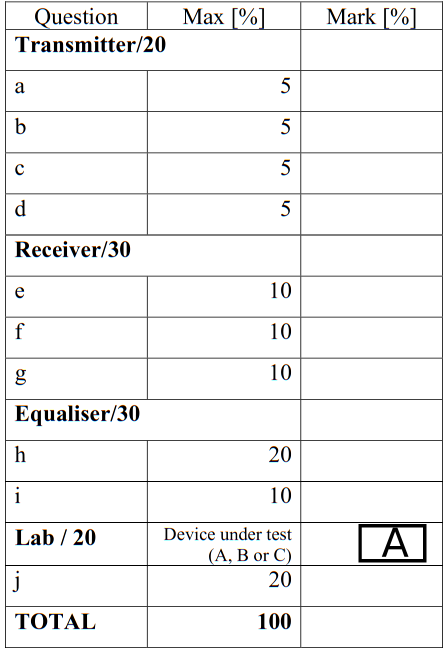
\includegraphics[width=0.6\textwidth, keepaspectratio]{marks_table.png}
\end{center}
\newpage
\section{Modulation type feasibility}
\section{Power spectral density of 4-PAM}\label{rect_psd_section}
The power spectral density of a pulse-shaped data sequence is given by the
energy spectral density of the pulse shape multiplied by power spectral density
of the impulse chain (data sequence). The power spectral density of the impulse
chain can be found be calculating the Fourier transform of the autocorrelation
of the impulse chain.
\begin{equation}
    S_y(f) = |P(f)|^2S_x(f) = |P(f)|^2 \mathcal{F} \{ R_x(\tau) \}
\end{equation}
$R_x(\tau)$ is a continuous autocorrelation, but due to the fact that the data
is comprised of delta functions, $R_x(\tau)$ will only be non-zero when these
delta functions line up, ie. when $\tau$ is an integer multiple of the sampling
period $T_s$. Because of this, $R_x(\tau)$ can be represented as a sum rather
than an integral.

$R_n$ represents the value of the autocorrelation at an integer sample offset of
$n$. $N$ represents the window size in units of samples ($N = \frac{T}{T_s}$).
\begin{equation}\label{rn}
    R_n = \lim_{N \to \infty}  \frac{1}{N} \sum_{k} a_k a_{k-n}
\end{equation}

Since the continuous time correlation is only non-zero at multiples of sample
period, it can be represented as an impulse chain (ie. sum of time-offset delta
functions), where the height of each delta function is given by the discreet
autocorrelation value at that offset.
\begin{equation}\label{autocorr}
    R_x(\tau) = \frac{1}{T_s} \sum_{n=-\infty}^{\infty} R_n \delta(\tau - nT_s)
\end{equation}

\subsection{Calculating $R_n$\label{calcrn}}
From \Cref{rn}, we can see that the discreet autocorrelation values are
dependent on two adjacent values of $x[n]$. No specific data sequence is given
in the question, so I will assume the input data is random. A table of all the
possible combinations of adjacent signals can be produced. Since this is 4-PAM,
the possible values for a single sample are $x[n] \in \{-3, -1, 1, 3\}$.
\begin{table}[H]
    \begin{center}
        \begin{tabular}{c|c c c c}
               & -3 & -1 & 1  & 3  \\
            \hline
            -3 & 9  & 3  & -3 & -9 \\
            -1 & 3  & 1  & -1 & -3 \\
            1  & -3 & -1 & 1  & 3  \\
            3  & -9 & -3 & 3  & 9
        \end{tabular}
    \end{center}
    \caption{Symbol combinations\label{combos}}
\end{table}
From \Cref{combos}, there are 16 possibilities for adjacent symbol
multiplication. $\pm\{1, 9\}$ occur twice each, while $\pm 3$ occur four
times each. Over a suffiently long dataset, the sum in \Cref{rn} will become an
average of all the combinations.
\begin{equation}
    \begin{gathered}
        \frac{1}{N} \sum_k a_k a_{k-n} = \frac{2}{16}(1) + \frac{2}{16}(-1) +
        \frac{2}{16}(9) + \frac{2}{16}(-9) + \frac{4}{16}(3) + \frac{4}{16}(-3)
        \\
        \frac{1}{N} \sum_k a_k a_{k-n} = 0
    \end{gathered}
\end{equation}

\subsection{Calculating $R_0$}
$R_0$ is the autocorrelation of the impulse chain at time of zero. The sum from
\Cref{rn} becomes
\begin{equation}
    \lim_{N \to \infty}  \frac{1}{N}\sum_k a_k^2
\end{equation}
Like in \Cref{calcrn}, it can be assumed that all possibilities of $\{-3, -1, 1,
    3\}$ are equally likelely, and the sum becomes the average.
\begin{equation}
    R_0 = \frac{1}{4}(-3)^2 + \frac{1}{4}(-1)^2 + \frac{1}{4}(1)^2 +
    \frac{1}{4}(3)^2 = 5
\end{equation}

\subsection{Calculating PSD}
From \Cref{autocorr}, since $R_n$ is zero for all $n\neq 0$:
\begin{equation}
    R_x(\tau) = R_0 \delta(\tau)
\end{equation}
\begin{equation}
    R_x(f) = \mathcal{F}\{\frac{5}{T_s} \delta(\tau)\} = \frac{5}{T_s} = S_x(f)
\end{equation}
\begin{equation}
    \begin{gathered}
        S_y(f) = |P(f)|^2S_x(f) = S_x(f) \int_{-\infty}^{\infty} rect(T_s)
        \,dt\\
        S_y(f) = \frac{5}{T_s}T_s = \boldsymbol 5
    \end{gathered}
\end{equation}


\section{Design of pulse shape}
A raised cosine filter is used for pulse shaping. Choose $B_T = 750KHz$ and
$\alpha = 1$ so that the filter produces maximum power transfer while staying
within the bandwidth limit.
\begin{figure}[H]
    \centering
    \scalebox{0.7}{%% Creator: Matplotlib, PGF backend
%%
%% To include the figure in your LaTeX document, write
%%   \input{<filename>.pgf}
%%
%% Make sure the required packages are loaded in your preamble
%%   \usepackage{pgf}
%%
%% Figures using additional raster images can only be included by \input if
%% they are in the same directory as the main LaTeX file. For loading figures
%% from other directories you can use the `import` package
%%   \usepackage{import}
%% and then include the figures with
%%   \import{<path to file>}{<filename>.pgf}
%%
%% Matplotlib used the following preamble
%%   \usepackage{fontspec}
%%   \setmainfont{DejaVuSerif.ttf}[Path=/usr/share/matplotlib/mpl-data/fonts/ttf/]
%%   \setsansfont{DejaVuSans.ttf}[Path=/usr/share/matplotlib/mpl-data/fonts/ttf/]
%%   \setmonofont{DejaVuSansMono.ttf}[Path=/usr/share/matplotlib/mpl-data/fonts/ttf/]
%%
\begingroup%
\makeatletter%
\begin{pgfpicture}%
\pgfpathrectangle{\pgfpointorigin}{\pgfqpoint{6.400000in}{4.800000in}}%
\pgfusepath{use as bounding box, clip}%
\begin{pgfscope}%
\pgfsetbuttcap%
\pgfsetmiterjoin%
\definecolor{currentfill}{rgb}{1.000000,1.000000,1.000000}%
\pgfsetfillcolor{currentfill}%
\pgfsetlinewidth{0.000000pt}%
\definecolor{currentstroke}{rgb}{1.000000,1.000000,1.000000}%
\pgfsetstrokecolor{currentstroke}%
\pgfsetdash{}{0pt}%
\pgfpathmoveto{\pgfqpoint{0.000000in}{0.000000in}}%
\pgfpathlineto{\pgfqpoint{6.400000in}{0.000000in}}%
\pgfpathlineto{\pgfqpoint{6.400000in}{4.800000in}}%
\pgfpathlineto{\pgfqpoint{0.000000in}{4.800000in}}%
\pgfpathclose%
\pgfusepath{fill}%
\end{pgfscope}%
\begin{pgfscope}%
\pgfsetbuttcap%
\pgfsetmiterjoin%
\definecolor{currentfill}{rgb}{1.000000,1.000000,1.000000}%
\pgfsetfillcolor{currentfill}%
\pgfsetlinewidth{0.000000pt}%
\definecolor{currentstroke}{rgb}{0.000000,0.000000,0.000000}%
\pgfsetstrokecolor{currentstroke}%
\pgfsetstrokeopacity{0.000000}%
\pgfsetdash{}{0pt}%
\pgfpathmoveto{\pgfqpoint{0.800000in}{0.528000in}}%
\pgfpathlineto{\pgfqpoint{5.760000in}{0.528000in}}%
\pgfpathlineto{\pgfqpoint{5.760000in}{4.224000in}}%
\pgfpathlineto{\pgfqpoint{0.800000in}{4.224000in}}%
\pgfpathclose%
\pgfusepath{fill}%
\end{pgfscope}%
\begin{pgfscope}%
\pgfpathrectangle{\pgfqpoint{0.800000in}{0.528000in}}{\pgfqpoint{4.960000in}{3.696000in}}%
\pgfusepath{clip}%
\pgfsetbuttcap%
\pgfsetmiterjoin%
\definecolor{currentfill}{rgb}{1.000000,0.498039,0.054902}%
\pgfsetfillcolor{currentfill}%
\pgfsetfillopacity{0.200000}%
\pgfsetlinewidth{0.000000pt}%
\definecolor{currentstroke}{rgb}{0.000000,0.000000,0.000000}%
\pgfsetstrokecolor{currentstroke}%
\pgfsetstrokeopacity{0.200000}%
\pgfsetdash{}{0pt}%
\pgfpathmoveto{\pgfqpoint{2.152727in}{0.528000in}}%
\pgfpathlineto{\pgfqpoint{2.152727in}{4.224000in}}%
\pgfpathlineto{\pgfqpoint{4.407273in}{4.224000in}}%
\pgfpathlineto{\pgfqpoint{4.407273in}{0.528000in}}%
\pgfpathclose%
\pgfusepath{fill}%
\end{pgfscope}%
\begin{pgfscope}%
\pgfpathrectangle{\pgfqpoint{0.800000in}{0.528000in}}{\pgfqpoint{4.960000in}{3.696000in}}%
\pgfusepath{clip}%
\pgfsetrectcap%
\pgfsetroundjoin%
\pgfsetlinewidth{0.803000pt}%
\definecolor{currentstroke}{rgb}{0.690196,0.690196,0.690196}%
\pgfsetstrokecolor{currentstroke}%
\pgfsetdash{}{0pt}%
\pgfpathmoveto{\pgfqpoint{1.025455in}{0.528000in}}%
\pgfpathlineto{\pgfqpoint{1.025455in}{4.224000in}}%
\pgfusepath{stroke}%
\end{pgfscope}%
\begin{pgfscope}%
\pgfsetbuttcap%
\pgfsetroundjoin%
\definecolor{currentfill}{rgb}{0.000000,0.000000,0.000000}%
\pgfsetfillcolor{currentfill}%
\pgfsetlinewidth{0.803000pt}%
\definecolor{currentstroke}{rgb}{0.000000,0.000000,0.000000}%
\pgfsetstrokecolor{currentstroke}%
\pgfsetdash{}{0pt}%
\pgfsys@defobject{currentmarker}{\pgfqpoint{0.000000in}{-0.048611in}}{\pgfqpoint{0.000000in}{0.000000in}}{%
\pgfpathmoveto{\pgfqpoint{0.000000in}{0.000000in}}%
\pgfpathlineto{\pgfqpoint{0.000000in}{-0.048611in}}%
\pgfusepath{stroke,fill}%
}%
\begin{pgfscope}%
\pgfsys@transformshift{1.025455in}{0.528000in}%
\pgfsys@useobject{currentmarker}{}%
\end{pgfscope}%
\end{pgfscope}%
\begin{pgfscope}%
\definecolor{textcolor}{rgb}{0.000000,0.000000,0.000000}%
\pgfsetstrokecolor{textcolor}%
\pgfsetfillcolor{textcolor}%
\pgftext[x=1.025455in,y=0.430778in,,top]{\color{textcolor}\sffamily\fontsize{10.000000}{12.000000}\selectfont −1.5}%
\end{pgfscope}%
\begin{pgfscope}%
\pgfpathrectangle{\pgfqpoint{0.800000in}{0.528000in}}{\pgfqpoint{4.960000in}{3.696000in}}%
\pgfusepath{clip}%
\pgfsetrectcap%
\pgfsetroundjoin%
\pgfsetlinewidth{0.803000pt}%
\definecolor{currentstroke}{rgb}{0.690196,0.690196,0.690196}%
\pgfsetstrokecolor{currentstroke}%
\pgfsetdash{}{0pt}%
\pgfpathmoveto{\pgfqpoint{1.776970in}{0.528000in}}%
\pgfpathlineto{\pgfqpoint{1.776970in}{4.224000in}}%
\pgfusepath{stroke}%
\end{pgfscope}%
\begin{pgfscope}%
\pgfsetbuttcap%
\pgfsetroundjoin%
\definecolor{currentfill}{rgb}{0.000000,0.000000,0.000000}%
\pgfsetfillcolor{currentfill}%
\pgfsetlinewidth{0.803000pt}%
\definecolor{currentstroke}{rgb}{0.000000,0.000000,0.000000}%
\pgfsetstrokecolor{currentstroke}%
\pgfsetdash{}{0pt}%
\pgfsys@defobject{currentmarker}{\pgfqpoint{0.000000in}{-0.048611in}}{\pgfqpoint{0.000000in}{0.000000in}}{%
\pgfpathmoveto{\pgfqpoint{0.000000in}{0.000000in}}%
\pgfpathlineto{\pgfqpoint{0.000000in}{-0.048611in}}%
\pgfusepath{stroke,fill}%
}%
\begin{pgfscope}%
\pgfsys@transformshift{1.776970in}{0.528000in}%
\pgfsys@useobject{currentmarker}{}%
\end{pgfscope}%
\end{pgfscope}%
\begin{pgfscope}%
\definecolor{textcolor}{rgb}{0.000000,0.000000,0.000000}%
\pgfsetstrokecolor{textcolor}%
\pgfsetfillcolor{textcolor}%
\pgftext[x=1.776970in,y=0.430778in,,top]{\color{textcolor}\sffamily\fontsize{10.000000}{12.000000}\selectfont −1.0}%
\end{pgfscope}%
\begin{pgfscope}%
\pgfpathrectangle{\pgfqpoint{0.800000in}{0.528000in}}{\pgfqpoint{4.960000in}{3.696000in}}%
\pgfusepath{clip}%
\pgfsetrectcap%
\pgfsetroundjoin%
\pgfsetlinewidth{0.803000pt}%
\definecolor{currentstroke}{rgb}{0.690196,0.690196,0.690196}%
\pgfsetstrokecolor{currentstroke}%
\pgfsetdash{}{0pt}%
\pgfpathmoveto{\pgfqpoint{2.528485in}{0.528000in}}%
\pgfpathlineto{\pgfqpoint{2.528485in}{4.224000in}}%
\pgfusepath{stroke}%
\end{pgfscope}%
\begin{pgfscope}%
\pgfsetbuttcap%
\pgfsetroundjoin%
\definecolor{currentfill}{rgb}{0.000000,0.000000,0.000000}%
\pgfsetfillcolor{currentfill}%
\pgfsetlinewidth{0.803000pt}%
\definecolor{currentstroke}{rgb}{0.000000,0.000000,0.000000}%
\pgfsetstrokecolor{currentstroke}%
\pgfsetdash{}{0pt}%
\pgfsys@defobject{currentmarker}{\pgfqpoint{0.000000in}{-0.048611in}}{\pgfqpoint{0.000000in}{0.000000in}}{%
\pgfpathmoveto{\pgfqpoint{0.000000in}{0.000000in}}%
\pgfpathlineto{\pgfqpoint{0.000000in}{-0.048611in}}%
\pgfusepath{stroke,fill}%
}%
\begin{pgfscope}%
\pgfsys@transformshift{2.528485in}{0.528000in}%
\pgfsys@useobject{currentmarker}{}%
\end{pgfscope}%
\end{pgfscope}%
\begin{pgfscope}%
\definecolor{textcolor}{rgb}{0.000000,0.000000,0.000000}%
\pgfsetstrokecolor{textcolor}%
\pgfsetfillcolor{textcolor}%
\pgftext[x=2.528485in,y=0.430778in,,top]{\color{textcolor}\sffamily\fontsize{10.000000}{12.000000}\selectfont −0.5}%
\end{pgfscope}%
\begin{pgfscope}%
\pgfpathrectangle{\pgfqpoint{0.800000in}{0.528000in}}{\pgfqpoint{4.960000in}{3.696000in}}%
\pgfusepath{clip}%
\pgfsetrectcap%
\pgfsetroundjoin%
\pgfsetlinewidth{0.803000pt}%
\definecolor{currentstroke}{rgb}{0.690196,0.690196,0.690196}%
\pgfsetstrokecolor{currentstroke}%
\pgfsetdash{}{0pt}%
\pgfpathmoveto{\pgfqpoint{3.280000in}{0.528000in}}%
\pgfpathlineto{\pgfqpoint{3.280000in}{4.224000in}}%
\pgfusepath{stroke}%
\end{pgfscope}%
\begin{pgfscope}%
\pgfsetbuttcap%
\pgfsetroundjoin%
\definecolor{currentfill}{rgb}{0.000000,0.000000,0.000000}%
\pgfsetfillcolor{currentfill}%
\pgfsetlinewidth{0.803000pt}%
\definecolor{currentstroke}{rgb}{0.000000,0.000000,0.000000}%
\pgfsetstrokecolor{currentstroke}%
\pgfsetdash{}{0pt}%
\pgfsys@defobject{currentmarker}{\pgfqpoint{0.000000in}{-0.048611in}}{\pgfqpoint{0.000000in}{0.000000in}}{%
\pgfpathmoveto{\pgfqpoint{0.000000in}{0.000000in}}%
\pgfpathlineto{\pgfqpoint{0.000000in}{-0.048611in}}%
\pgfusepath{stroke,fill}%
}%
\begin{pgfscope}%
\pgfsys@transformshift{3.280000in}{0.528000in}%
\pgfsys@useobject{currentmarker}{}%
\end{pgfscope}%
\end{pgfscope}%
\begin{pgfscope}%
\definecolor{textcolor}{rgb}{0.000000,0.000000,0.000000}%
\pgfsetstrokecolor{textcolor}%
\pgfsetfillcolor{textcolor}%
\pgftext[x=3.280000in,y=0.430778in,,top]{\color{textcolor}\sffamily\fontsize{10.000000}{12.000000}\selectfont 0.0}%
\end{pgfscope}%
\begin{pgfscope}%
\pgfpathrectangle{\pgfqpoint{0.800000in}{0.528000in}}{\pgfqpoint{4.960000in}{3.696000in}}%
\pgfusepath{clip}%
\pgfsetrectcap%
\pgfsetroundjoin%
\pgfsetlinewidth{0.803000pt}%
\definecolor{currentstroke}{rgb}{0.690196,0.690196,0.690196}%
\pgfsetstrokecolor{currentstroke}%
\pgfsetdash{}{0pt}%
\pgfpathmoveto{\pgfqpoint{4.031515in}{0.528000in}}%
\pgfpathlineto{\pgfqpoint{4.031515in}{4.224000in}}%
\pgfusepath{stroke}%
\end{pgfscope}%
\begin{pgfscope}%
\pgfsetbuttcap%
\pgfsetroundjoin%
\definecolor{currentfill}{rgb}{0.000000,0.000000,0.000000}%
\pgfsetfillcolor{currentfill}%
\pgfsetlinewidth{0.803000pt}%
\definecolor{currentstroke}{rgb}{0.000000,0.000000,0.000000}%
\pgfsetstrokecolor{currentstroke}%
\pgfsetdash{}{0pt}%
\pgfsys@defobject{currentmarker}{\pgfqpoint{0.000000in}{-0.048611in}}{\pgfqpoint{0.000000in}{0.000000in}}{%
\pgfpathmoveto{\pgfqpoint{0.000000in}{0.000000in}}%
\pgfpathlineto{\pgfqpoint{0.000000in}{-0.048611in}}%
\pgfusepath{stroke,fill}%
}%
\begin{pgfscope}%
\pgfsys@transformshift{4.031515in}{0.528000in}%
\pgfsys@useobject{currentmarker}{}%
\end{pgfscope}%
\end{pgfscope}%
\begin{pgfscope}%
\definecolor{textcolor}{rgb}{0.000000,0.000000,0.000000}%
\pgfsetstrokecolor{textcolor}%
\pgfsetfillcolor{textcolor}%
\pgftext[x=4.031515in,y=0.430778in,,top]{\color{textcolor}\sffamily\fontsize{10.000000}{12.000000}\selectfont 0.5}%
\end{pgfscope}%
\begin{pgfscope}%
\pgfpathrectangle{\pgfqpoint{0.800000in}{0.528000in}}{\pgfqpoint{4.960000in}{3.696000in}}%
\pgfusepath{clip}%
\pgfsetrectcap%
\pgfsetroundjoin%
\pgfsetlinewidth{0.803000pt}%
\definecolor{currentstroke}{rgb}{0.690196,0.690196,0.690196}%
\pgfsetstrokecolor{currentstroke}%
\pgfsetdash{}{0pt}%
\pgfpathmoveto{\pgfqpoint{4.783030in}{0.528000in}}%
\pgfpathlineto{\pgfqpoint{4.783030in}{4.224000in}}%
\pgfusepath{stroke}%
\end{pgfscope}%
\begin{pgfscope}%
\pgfsetbuttcap%
\pgfsetroundjoin%
\definecolor{currentfill}{rgb}{0.000000,0.000000,0.000000}%
\pgfsetfillcolor{currentfill}%
\pgfsetlinewidth{0.803000pt}%
\definecolor{currentstroke}{rgb}{0.000000,0.000000,0.000000}%
\pgfsetstrokecolor{currentstroke}%
\pgfsetdash{}{0pt}%
\pgfsys@defobject{currentmarker}{\pgfqpoint{0.000000in}{-0.048611in}}{\pgfqpoint{0.000000in}{0.000000in}}{%
\pgfpathmoveto{\pgfqpoint{0.000000in}{0.000000in}}%
\pgfpathlineto{\pgfqpoint{0.000000in}{-0.048611in}}%
\pgfusepath{stroke,fill}%
}%
\begin{pgfscope}%
\pgfsys@transformshift{4.783030in}{0.528000in}%
\pgfsys@useobject{currentmarker}{}%
\end{pgfscope}%
\end{pgfscope}%
\begin{pgfscope}%
\definecolor{textcolor}{rgb}{0.000000,0.000000,0.000000}%
\pgfsetstrokecolor{textcolor}%
\pgfsetfillcolor{textcolor}%
\pgftext[x=4.783030in,y=0.430778in,,top]{\color{textcolor}\sffamily\fontsize{10.000000}{12.000000}\selectfont 1.0}%
\end{pgfscope}%
\begin{pgfscope}%
\pgfpathrectangle{\pgfqpoint{0.800000in}{0.528000in}}{\pgfqpoint{4.960000in}{3.696000in}}%
\pgfusepath{clip}%
\pgfsetrectcap%
\pgfsetroundjoin%
\pgfsetlinewidth{0.803000pt}%
\definecolor{currentstroke}{rgb}{0.690196,0.690196,0.690196}%
\pgfsetstrokecolor{currentstroke}%
\pgfsetdash{}{0pt}%
\pgfpathmoveto{\pgfqpoint{5.534545in}{0.528000in}}%
\pgfpathlineto{\pgfqpoint{5.534545in}{4.224000in}}%
\pgfusepath{stroke}%
\end{pgfscope}%
\begin{pgfscope}%
\pgfsetbuttcap%
\pgfsetroundjoin%
\definecolor{currentfill}{rgb}{0.000000,0.000000,0.000000}%
\pgfsetfillcolor{currentfill}%
\pgfsetlinewidth{0.803000pt}%
\definecolor{currentstroke}{rgb}{0.000000,0.000000,0.000000}%
\pgfsetstrokecolor{currentstroke}%
\pgfsetdash{}{0pt}%
\pgfsys@defobject{currentmarker}{\pgfqpoint{0.000000in}{-0.048611in}}{\pgfqpoint{0.000000in}{0.000000in}}{%
\pgfpathmoveto{\pgfqpoint{0.000000in}{0.000000in}}%
\pgfpathlineto{\pgfqpoint{0.000000in}{-0.048611in}}%
\pgfusepath{stroke,fill}%
}%
\begin{pgfscope}%
\pgfsys@transformshift{5.534545in}{0.528000in}%
\pgfsys@useobject{currentmarker}{}%
\end{pgfscope}%
\end{pgfscope}%
\begin{pgfscope}%
\definecolor{textcolor}{rgb}{0.000000,0.000000,0.000000}%
\pgfsetstrokecolor{textcolor}%
\pgfsetfillcolor{textcolor}%
\pgftext[x=5.534545in,y=0.430778in,,top]{\color{textcolor}\sffamily\fontsize{10.000000}{12.000000}\selectfont 1.5}%
\end{pgfscope}%
\begin{pgfscope}%
\definecolor{textcolor}{rgb}{0.000000,0.000000,0.000000}%
\pgfsetstrokecolor{textcolor}%
\pgfsetfillcolor{textcolor}%
\pgftext[x=3.280000in,y=0.240809in,,top]{\color{textcolor}\sffamily\fontsize{10.000000}{12.000000}\selectfont Frequency (Hz)}%
\end{pgfscope}%
\begin{pgfscope}%
\definecolor{textcolor}{rgb}{0.000000,0.000000,0.000000}%
\pgfsetstrokecolor{textcolor}%
\pgfsetfillcolor{textcolor}%
\pgftext[x=5.760000in,y=0.254698in,right,top]{\color{textcolor}\sffamily\fontsize{10.000000}{12.000000}\selectfont 1e6}%
\end{pgfscope}%
\begin{pgfscope}%
\pgfpathrectangle{\pgfqpoint{0.800000in}{0.528000in}}{\pgfqpoint{4.960000in}{3.696000in}}%
\pgfusepath{clip}%
\pgfsetrectcap%
\pgfsetroundjoin%
\pgfsetlinewidth{0.803000pt}%
\definecolor{currentstroke}{rgb}{0.690196,0.690196,0.690196}%
\pgfsetstrokecolor{currentstroke}%
\pgfsetdash{}{0pt}%
\pgfpathmoveto{\pgfqpoint{0.800000in}{0.696000in}}%
\pgfpathlineto{\pgfqpoint{5.760000in}{0.696000in}}%
\pgfusepath{stroke}%
\end{pgfscope}%
\begin{pgfscope}%
\pgfsetbuttcap%
\pgfsetroundjoin%
\definecolor{currentfill}{rgb}{0.000000,0.000000,0.000000}%
\pgfsetfillcolor{currentfill}%
\pgfsetlinewidth{0.803000pt}%
\definecolor{currentstroke}{rgb}{0.000000,0.000000,0.000000}%
\pgfsetstrokecolor{currentstroke}%
\pgfsetdash{}{0pt}%
\pgfsys@defobject{currentmarker}{\pgfqpoint{-0.048611in}{0.000000in}}{\pgfqpoint{0.000000in}{0.000000in}}{%
\pgfpathmoveto{\pgfqpoint{0.000000in}{0.000000in}}%
\pgfpathlineto{\pgfqpoint{-0.048611in}{0.000000in}}%
\pgfusepath{stroke,fill}%
}%
\begin{pgfscope}%
\pgfsys@transformshift{0.800000in}{0.696000in}%
\pgfsys@useobject{currentmarker}{}%
\end{pgfscope}%
\end{pgfscope}%
\begin{pgfscope}%
\definecolor{textcolor}{rgb}{0.000000,0.000000,0.000000}%
\pgfsetstrokecolor{textcolor}%
\pgfsetfillcolor{textcolor}%
\pgftext[x=0.481898in,y=0.643238in,left,base]{\color{textcolor}\sffamily\fontsize{10.000000}{12.000000}\selectfont 0.0}%
\end{pgfscope}%
\begin{pgfscope}%
\pgfpathrectangle{\pgfqpoint{0.800000in}{0.528000in}}{\pgfqpoint{4.960000in}{3.696000in}}%
\pgfusepath{clip}%
\pgfsetrectcap%
\pgfsetroundjoin%
\pgfsetlinewidth{0.803000pt}%
\definecolor{currentstroke}{rgb}{0.690196,0.690196,0.690196}%
\pgfsetstrokecolor{currentstroke}%
\pgfsetdash{}{0pt}%
\pgfpathmoveto{\pgfqpoint{0.800000in}{1.200020in}}%
\pgfpathlineto{\pgfqpoint{5.760000in}{1.200020in}}%
\pgfusepath{stroke}%
\end{pgfscope}%
\begin{pgfscope}%
\pgfsetbuttcap%
\pgfsetroundjoin%
\definecolor{currentfill}{rgb}{0.000000,0.000000,0.000000}%
\pgfsetfillcolor{currentfill}%
\pgfsetlinewidth{0.803000pt}%
\definecolor{currentstroke}{rgb}{0.000000,0.000000,0.000000}%
\pgfsetstrokecolor{currentstroke}%
\pgfsetdash{}{0pt}%
\pgfsys@defobject{currentmarker}{\pgfqpoint{-0.048611in}{0.000000in}}{\pgfqpoint{0.000000in}{0.000000in}}{%
\pgfpathmoveto{\pgfqpoint{0.000000in}{0.000000in}}%
\pgfpathlineto{\pgfqpoint{-0.048611in}{0.000000in}}%
\pgfusepath{stroke,fill}%
}%
\begin{pgfscope}%
\pgfsys@transformshift{0.800000in}{1.200020in}%
\pgfsys@useobject{currentmarker}{}%
\end{pgfscope}%
\end{pgfscope}%
\begin{pgfscope}%
\definecolor{textcolor}{rgb}{0.000000,0.000000,0.000000}%
\pgfsetstrokecolor{textcolor}%
\pgfsetfillcolor{textcolor}%
\pgftext[x=0.481898in,y=1.147258in,left,base]{\color{textcolor}\sffamily\fontsize{10.000000}{12.000000}\selectfont 0.2}%
\end{pgfscope}%
\begin{pgfscope}%
\pgfpathrectangle{\pgfqpoint{0.800000in}{0.528000in}}{\pgfqpoint{4.960000in}{3.696000in}}%
\pgfusepath{clip}%
\pgfsetrectcap%
\pgfsetroundjoin%
\pgfsetlinewidth{0.803000pt}%
\definecolor{currentstroke}{rgb}{0.690196,0.690196,0.690196}%
\pgfsetstrokecolor{currentstroke}%
\pgfsetdash{}{0pt}%
\pgfpathmoveto{\pgfqpoint{0.800000in}{1.704040in}}%
\pgfpathlineto{\pgfqpoint{5.760000in}{1.704040in}}%
\pgfusepath{stroke}%
\end{pgfscope}%
\begin{pgfscope}%
\pgfsetbuttcap%
\pgfsetroundjoin%
\definecolor{currentfill}{rgb}{0.000000,0.000000,0.000000}%
\pgfsetfillcolor{currentfill}%
\pgfsetlinewidth{0.803000pt}%
\definecolor{currentstroke}{rgb}{0.000000,0.000000,0.000000}%
\pgfsetstrokecolor{currentstroke}%
\pgfsetdash{}{0pt}%
\pgfsys@defobject{currentmarker}{\pgfqpoint{-0.048611in}{0.000000in}}{\pgfqpoint{0.000000in}{0.000000in}}{%
\pgfpathmoveto{\pgfqpoint{0.000000in}{0.000000in}}%
\pgfpathlineto{\pgfqpoint{-0.048611in}{0.000000in}}%
\pgfusepath{stroke,fill}%
}%
\begin{pgfscope}%
\pgfsys@transformshift{0.800000in}{1.704040in}%
\pgfsys@useobject{currentmarker}{}%
\end{pgfscope}%
\end{pgfscope}%
\begin{pgfscope}%
\definecolor{textcolor}{rgb}{0.000000,0.000000,0.000000}%
\pgfsetstrokecolor{textcolor}%
\pgfsetfillcolor{textcolor}%
\pgftext[x=0.481898in,y=1.651278in,left,base]{\color{textcolor}\sffamily\fontsize{10.000000}{12.000000}\selectfont 0.4}%
\end{pgfscope}%
\begin{pgfscope}%
\pgfpathrectangle{\pgfqpoint{0.800000in}{0.528000in}}{\pgfqpoint{4.960000in}{3.696000in}}%
\pgfusepath{clip}%
\pgfsetrectcap%
\pgfsetroundjoin%
\pgfsetlinewidth{0.803000pt}%
\definecolor{currentstroke}{rgb}{0.690196,0.690196,0.690196}%
\pgfsetstrokecolor{currentstroke}%
\pgfsetdash{}{0pt}%
\pgfpathmoveto{\pgfqpoint{0.800000in}{2.208060in}}%
\pgfpathlineto{\pgfqpoint{5.760000in}{2.208060in}}%
\pgfusepath{stroke}%
\end{pgfscope}%
\begin{pgfscope}%
\pgfsetbuttcap%
\pgfsetroundjoin%
\definecolor{currentfill}{rgb}{0.000000,0.000000,0.000000}%
\pgfsetfillcolor{currentfill}%
\pgfsetlinewidth{0.803000pt}%
\definecolor{currentstroke}{rgb}{0.000000,0.000000,0.000000}%
\pgfsetstrokecolor{currentstroke}%
\pgfsetdash{}{0pt}%
\pgfsys@defobject{currentmarker}{\pgfqpoint{-0.048611in}{0.000000in}}{\pgfqpoint{0.000000in}{0.000000in}}{%
\pgfpathmoveto{\pgfqpoint{0.000000in}{0.000000in}}%
\pgfpathlineto{\pgfqpoint{-0.048611in}{0.000000in}}%
\pgfusepath{stroke,fill}%
}%
\begin{pgfscope}%
\pgfsys@transformshift{0.800000in}{2.208060in}%
\pgfsys@useobject{currentmarker}{}%
\end{pgfscope}%
\end{pgfscope}%
\begin{pgfscope}%
\definecolor{textcolor}{rgb}{0.000000,0.000000,0.000000}%
\pgfsetstrokecolor{textcolor}%
\pgfsetfillcolor{textcolor}%
\pgftext[x=0.481898in,y=2.155298in,left,base]{\color{textcolor}\sffamily\fontsize{10.000000}{12.000000}\selectfont 0.6}%
\end{pgfscope}%
\begin{pgfscope}%
\pgfpathrectangle{\pgfqpoint{0.800000in}{0.528000in}}{\pgfqpoint{4.960000in}{3.696000in}}%
\pgfusepath{clip}%
\pgfsetrectcap%
\pgfsetroundjoin%
\pgfsetlinewidth{0.803000pt}%
\definecolor{currentstroke}{rgb}{0.690196,0.690196,0.690196}%
\pgfsetstrokecolor{currentstroke}%
\pgfsetdash{}{0pt}%
\pgfpathmoveto{\pgfqpoint{0.800000in}{2.712080in}}%
\pgfpathlineto{\pgfqpoint{5.760000in}{2.712080in}}%
\pgfusepath{stroke}%
\end{pgfscope}%
\begin{pgfscope}%
\pgfsetbuttcap%
\pgfsetroundjoin%
\definecolor{currentfill}{rgb}{0.000000,0.000000,0.000000}%
\pgfsetfillcolor{currentfill}%
\pgfsetlinewidth{0.803000pt}%
\definecolor{currentstroke}{rgb}{0.000000,0.000000,0.000000}%
\pgfsetstrokecolor{currentstroke}%
\pgfsetdash{}{0pt}%
\pgfsys@defobject{currentmarker}{\pgfqpoint{-0.048611in}{0.000000in}}{\pgfqpoint{0.000000in}{0.000000in}}{%
\pgfpathmoveto{\pgfqpoint{0.000000in}{0.000000in}}%
\pgfpathlineto{\pgfqpoint{-0.048611in}{0.000000in}}%
\pgfusepath{stroke,fill}%
}%
\begin{pgfscope}%
\pgfsys@transformshift{0.800000in}{2.712080in}%
\pgfsys@useobject{currentmarker}{}%
\end{pgfscope}%
\end{pgfscope}%
\begin{pgfscope}%
\definecolor{textcolor}{rgb}{0.000000,0.000000,0.000000}%
\pgfsetstrokecolor{textcolor}%
\pgfsetfillcolor{textcolor}%
\pgftext[x=0.481898in,y=2.659318in,left,base]{\color{textcolor}\sffamily\fontsize{10.000000}{12.000000}\selectfont 0.8}%
\end{pgfscope}%
\begin{pgfscope}%
\pgfpathrectangle{\pgfqpoint{0.800000in}{0.528000in}}{\pgfqpoint{4.960000in}{3.696000in}}%
\pgfusepath{clip}%
\pgfsetrectcap%
\pgfsetroundjoin%
\pgfsetlinewidth{0.803000pt}%
\definecolor{currentstroke}{rgb}{0.690196,0.690196,0.690196}%
\pgfsetstrokecolor{currentstroke}%
\pgfsetdash{}{0pt}%
\pgfpathmoveto{\pgfqpoint{0.800000in}{3.216100in}}%
\pgfpathlineto{\pgfqpoint{5.760000in}{3.216100in}}%
\pgfusepath{stroke}%
\end{pgfscope}%
\begin{pgfscope}%
\pgfsetbuttcap%
\pgfsetroundjoin%
\definecolor{currentfill}{rgb}{0.000000,0.000000,0.000000}%
\pgfsetfillcolor{currentfill}%
\pgfsetlinewidth{0.803000pt}%
\definecolor{currentstroke}{rgb}{0.000000,0.000000,0.000000}%
\pgfsetstrokecolor{currentstroke}%
\pgfsetdash{}{0pt}%
\pgfsys@defobject{currentmarker}{\pgfqpoint{-0.048611in}{0.000000in}}{\pgfqpoint{0.000000in}{0.000000in}}{%
\pgfpathmoveto{\pgfqpoint{0.000000in}{0.000000in}}%
\pgfpathlineto{\pgfqpoint{-0.048611in}{0.000000in}}%
\pgfusepath{stroke,fill}%
}%
\begin{pgfscope}%
\pgfsys@transformshift{0.800000in}{3.216100in}%
\pgfsys@useobject{currentmarker}{}%
\end{pgfscope}%
\end{pgfscope}%
\begin{pgfscope}%
\definecolor{textcolor}{rgb}{0.000000,0.000000,0.000000}%
\pgfsetstrokecolor{textcolor}%
\pgfsetfillcolor{textcolor}%
\pgftext[x=0.481898in,y=3.163338in,left,base]{\color{textcolor}\sffamily\fontsize{10.000000}{12.000000}\selectfont 1.0}%
\end{pgfscope}%
\begin{pgfscope}%
\pgfpathrectangle{\pgfqpoint{0.800000in}{0.528000in}}{\pgfqpoint{4.960000in}{3.696000in}}%
\pgfusepath{clip}%
\pgfsetrectcap%
\pgfsetroundjoin%
\pgfsetlinewidth{0.803000pt}%
\definecolor{currentstroke}{rgb}{0.690196,0.690196,0.690196}%
\pgfsetstrokecolor{currentstroke}%
\pgfsetdash{}{0pt}%
\pgfpathmoveto{\pgfqpoint{0.800000in}{3.720120in}}%
\pgfpathlineto{\pgfqpoint{5.760000in}{3.720120in}}%
\pgfusepath{stroke}%
\end{pgfscope}%
\begin{pgfscope}%
\pgfsetbuttcap%
\pgfsetroundjoin%
\definecolor{currentfill}{rgb}{0.000000,0.000000,0.000000}%
\pgfsetfillcolor{currentfill}%
\pgfsetlinewidth{0.803000pt}%
\definecolor{currentstroke}{rgb}{0.000000,0.000000,0.000000}%
\pgfsetstrokecolor{currentstroke}%
\pgfsetdash{}{0pt}%
\pgfsys@defobject{currentmarker}{\pgfqpoint{-0.048611in}{0.000000in}}{\pgfqpoint{0.000000in}{0.000000in}}{%
\pgfpathmoveto{\pgfqpoint{0.000000in}{0.000000in}}%
\pgfpathlineto{\pgfqpoint{-0.048611in}{0.000000in}}%
\pgfusepath{stroke,fill}%
}%
\begin{pgfscope}%
\pgfsys@transformshift{0.800000in}{3.720120in}%
\pgfsys@useobject{currentmarker}{}%
\end{pgfscope}%
\end{pgfscope}%
\begin{pgfscope}%
\definecolor{textcolor}{rgb}{0.000000,0.000000,0.000000}%
\pgfsetstrokecolor{textcolor}%
\pgfsetfillcolor{textcolor}%
\pgftext[x=0.481898in,y=3.667358in,left,base]{\color{textcolor}\sffamily\fontsize{10.000000}{12.000000}\selectfont 1.2}%
\end{pgfscope}%
\begin{pgfscope}%
\definecolor{textcolor}{rgb}{0.000000,0.000000,0.000000}%
\pgfsetstrokecolor{textcolor}%
\pgfsetfillcolor{textcolor}%
\pgftext[x=0.800000in,y=4.265667in,left,base]{\color{textcolor}\sffamily\fontsize{10.000000}{12.000000}\selectfont 1e−6}%
\end{pgfscope}%
\begin{pgfscope}%
\pgfpathrectangle{\pgfqpoint{0.800000in}{0.528000in}}{\pgfqpoint{4.960000in}{3.696000in}}%
\pgfusepath{clip}%
\pgfsetrectcap%
\pgfsetroundjoin%
\pgfsetlinewidth{1.505625pt}%
\definecolor{currentstroke}{rgb}{0.121569,0.466667,0.705882}%
\pgfsetstrokecolor{currentstroke}%
\pgfsetdash{}{0pt}%
\pgfpathmoveto{\pgfqpoint{1.025455in}{0.696000in}}%
\pgfpathlineto{\pgfqpoint{2.164023in}{0.696832in}}%
\pgfpathlineto{\pgfqpoint{2.182095in}{0.701624in}}%
\pgfpathlineto{\pgfqpoint{2.200168in}{0.710662in}}%
\pgfpathlineto{\pgfqpoint{2.218240in}{0.723924in}}%
\pgfpathlineto{\pgfqpoint{2.236313in}{0.741377in}}%
\pgfpathlineto{\pgfqpoint{2.254385in}{0.762975in}}%
\pgfpathlineto{\pgfqpoint{2.272458in}{0.788665in}}%
\pgfpathlineto{\pgfqpoint{2.290530in}{0.818380in}}%
\pgfpathlineto{\pgfqpoint{2.308603in}{0.852046in}}%
\pgfpathlineto{\pgfqpoint{2.326675in}{0.889577in}}%
\pgfpathlineto{\pgfqpoint{2.344748in}{0.930879in}}%
\pgfpathlineto{\pgfqpoint{2.371856in}{0.999668in}}%
\pgfpathlineto{\pgfqpoint{2.398965in}{1.076310in}}%
\pgfpathlineto{\pgfqpoint{2.426074in}{1.160366in}}%
\pgfpathlineto{\pgfqpoint{2.453183in}{1.251359in}}%
\pgfpathlineto{\pgfqpoint{2.480291in}{1.348767in}}%
\pgfpathlineto{\pgfqpoint{2.516437in}{1.487661in}}%
\pgfpathlineto{\pgfqpoint{2.552582in}{1.635562in}}%
\pgfpathlineto{\pgfqpoint{2.597763in}{1.830813in}}%
\pgfpathlineto{\pgfqpoint{2.651980in}{2.076228in}}%
\pgfpathlineto{\pgfqpoint{2.850778in}{2.990801in}}%
\pgfpathlineto{\pgfqpoint{2.895959in}{3.182292in}}%
\pgfpathlineto{\pgfqpoint{2.932104in}{3.326431in}}%
\pgfpathlineto{\pgfqpoint{2.968249in}{3.460936in}}%
\pgfpathlineto{\pgfqpoint{2.995358in}{3.554667in}}%
\pgfpathlineto{\pgfqpoint{3.022467in}{3.641674in}}%
\pgfpathlineto{\pgfqpoint{3.049576in}{3.721461in}}%
\pgfpathlineto{\pgfqpoint{3.076684in}{3.793573in}}%
\pgfpathlineto{\pgfqpoint{3.103793in}{3.857597in}}%
\pgfpathlineto{\pgfqpoint{3.121866in}{3.895605in}}%
\pgfpathlineto{\pgfqpoint{3.139938in}{3.929759in}}%
\pgfpathlineto{\pgfqpoint{3.158011in}{3.959973in}}%
\pgfpathlineto{\pgfqpoint{3.176083in}{3.986169in}}%
\pgfpathlineto{\pgfqpoint{3.194156in}{4.008282in}}%
\pgfpathlineto{\pgfqpoint{3.212228in}{4.026256in}}%
\pgfpathlineto{\pgfqpoint{3.230301in}{4.040044in}}%
\pgfpathlineto{\pgfqpoint{3.248373in}{4.049611in}}%
\pgfpathlineto{\pgfqpoint{3.266446in}{4.054935in}}%
\pgfpathlineto{\pgfqpoint{3.284518in}{4.056000in}}%
\pgfpathlineto{\pgfqpoint{3.302591in}{4.052805in}}%
\pgfpathlineto{\pgfqpoint{3.320663in}{4.045357in}}%
\pgfpathlineto{\pgfqpoint{3.338736in}{4.033675in}}%
\pgfpathlineto{\pgfqpoint{3.356808in}{4.017789in}}%
\pgfpathlineto{\pgfqpoint{3.374881in}{3.997740in}}%
\pgfpathlineto{\pgfqpoint{3.392953in}{3.973578in}}%
\pgfpathlineto{\pgfqpoint{3.411026in}{3.945364in}}%
\pgfpathlineto{\pgfqpoint{3.429098in}{3.913170in}}%
\pgfpathlineto{\pgfqpoint{3.447171in}{3.877077in}}%
\pgfpathlineto{\pgfqpoint{3.465243in}{3.837178in}}%
\pgfpathlineto{\pgfqpoint{3.492352in}{3.770415in}}%
\pgfpathlineto{\pgfqpoint{3.519461in}{3.695697in}}%
\pgfpathlineto{\pgfqpoint{3.546570in}{3.613451in}}%
\pgfpathlineto{\pgfqpoint{3.573678in}{3.524145in}}%
\pgfpathlineto{\pgfqpoint{3.600787in}{3.428290in}}%
\pgfpathlineto{\pgfqpoint{3.636932in}{3.291244in}}%
\pgfpathlineto{\pgfqpoint{3.673077in}{3.144920in}}%
\pgfpathlineto{\pgfqpoint{3.718258in}{2.951235in}}%
\pgfpathlineto{\pgfqpoint{3.772476in}{2.707073in}}%
\pgfpathlineto{\pgfqpoint{3.862838in}{2.286202in}}%
\pgfpathlineto{\pgfqpoint{3.944165in}{1.911509in}}%
\pgfpathlineto{\pgfqpoint{3.989346in}{1.712425in}}%
\pgfpathlineto{\pgfqpoint{4.034527in}{1.523849in}}%
\pgfpathlineto{\pgfqpoint{4.070672in}{1.382568in}}%
\pgfpathlineto{\pgfqpoint{4.106817in}{1.251359in}}%
\pgfpathlineto{\pgfqpoint{4.133926in}{1.160366in}}%
\pgfpathlineto{\pgfqpoint{4.161035in}{1.076310in}}%
\pgfpathlineto{\pgfqpoint{4.188144in}{0.999668in}}%
\pgfpathlineto{\pgfqpoint{4.215252in}{0.930879in}}%
\pgfpathlineto{\pgfqpoint{4.242361in}{0.870334in}}%
\pgfpathlineto{\pgfqpoint{4.260434in}{0.834724in}}%
\pgfpathlineto{\pgfqpoint{4.278506in}{0.803024in}}%
\pgfpathlineto{\pgfqpoint{4.296579in}{0.775312in}}%
\pgfpathlineto{\pgfqpoint{4.314651in}{0.751661in}}%
\pgfpathlineto{\pgfqpoint{4.332724in}{0.732129in}}%
\pgfpathlineto{\pgfqpoint{4.350796in}{0.716767in}}%
\pgfpathlineto{\pgfqpoint{4.368869in}{0.705613in}}%
\pgfpathlineto{\pgfqpoint{4.386941in}{0.698696in}}%
\pgfpathlineto{\pgfqpoint{4.405014in}{0.696033in}}%
\pgfpathlineto{\pgfqpoint{4.712246in}{0.696000in}}%
\pgfpathlineto{\pgfqpoint{5.534545in}{0.696000in}}%
\pgfpathlineto{\pgfqpoint{5.534545in}{0.696000in}}%
\pgfusepath{stroke}%
\end{pgfscope}%
\begin{pgfscope}%
\pgfsetrectcap%
\pgfsetmiterjoin%
\pgfsetlinewidth{0.803000pt}%
\definecolor{currentstroke}{rgb}{0.000000,0.000000,0.000000}%
\pgfsetstrokecolor{currentstroke}%
\pgfsetdash{}{0pt}%
\pgfpathmoveto{\pgfqpoint{0.800000in}{0.528000in}}%
\pgfpathlineto{\pgfqpoint{0.800000in}{4.224000in}}%
\pgfusepath{stroke}%
\end{pgfscope}%
\begin{pgfscope}%
\pgfsetrectcap%
\pgfsetmiterjoin%
\pgfsetlinewidth{0.803000pt}%
\definecolor{currentstroke}{rgb}{0.000000,0.000000,0.000000}%
\pgfsetstrokecolor{currentstroke}%
\pgfsetdash{}{0pt}%
\pgfpathmoveto{\pgfqpoint{5.760000in}{0.528000in}}%
\pgfpathlineto{\pgfqpoint{5.760000in}{4.224000in}}%
\pgfusepath{stroke}%
\end{pgfscope}%
\begin{pgfscope}%
\pgfsetrectcap%
\pgfsetmiterjoin%
\pgfsetlinewidth{0.803000pt}%
\definecolor{currentstroke}{rgb}{0.000000,0.000000,0.000000}%
\pgfsetstrokecolor{currentstroke}%
\pgfsetdash{}{0pt}%
\pgfpathmoveto{\pgfqpoint{0.800000in}{0.528000in}}%
\pgfpathlineto{\pgfqpoint{5.760000in}{0.528000in}}%
\pgfusepath{stroke}%
\end{pgfscope}%
\begin{pgfscope}%
\pgfsetrectcap%
\pgfsetmiterjoin%
\pgfsetlinewidth{0.803000pt}%
\definecolor{currentstroke}{rgb}{0.000000,0.000000,0.000000}%
\pgfsetstrokecolor{currentstroke}%
\pgfsetdash{}{0pt}%
\pgfpathmoveto{\pgfqpoint{0.800000in}{4.224000in}}%
\pgfpathlineto{\pgfqpoint{5.760000in}{4.224000in}}%
\pgfusepath{stroke}%
\end{pgfscope}%
\begin{pgfscope}%
\pgfsetbuttcap%
\pgfsetmiterjoin%
\definecolor{currentfill}{rgb}{1.000000,1.000000,1.000000}%
\pgfsetfillcolor{currentfill}%
\pgfsetfillopacity{0.800000}%
\pgfsetlinewidth{1.003750pt}%
\definecolor{currentstroke}{rgb}{0.800000,0.800000,0.800000}%
\pgfsetstrokecolor{currentstroke}%
\pgfsetstrokeopacity{0.800000}%
\pgfsetdash{}{0pt}%
\pgfpathmoveto{\pgfqpoint{4.129263in}{3.699342in}}%
\pgfpathlineto{\pgfqpoint{5.662778in}{3.699342in}}%
\pgfpathquadraticcurveto{\pgfqpoint{5.690556in}{3.699342in}}{\pgfqpoint{5.690556in}{3.727120in}}%
\pgfpathlineto{\pgfqpoint{5.690556in}{4.126778in}}%
\pgfpathquadraticcurveto{\pgfqpoint{5.690556in}{4.154556in}}{\pgfqpoint{5.662778in}{4.154556in}}%
\pgfpathlineto{\pgfqpoint{4.129263in}{4.154556in}}%
\pgfpathquadraticcurveto{\pgfqpoint{4.101485in}{4.154556in}}{\pgfqpoint{4.101485in}{4.126778in}}%
\pgfpathlineto{\pgfqpoint{4.101485in}{3.727120in}}%
\pgfpathquadraticcurveto{\pgfqpoint{4.101485in}{3.699342in}}{\pgfqpoint{4.129263in}{3.699342in}}%
\pgfpathclose%
\pgfusepath{stroke,fill}%
\end{pgfscope}%
\begin{pgfscope}%
\pgfsetrectcap%
\pgfsetroundjoin%
\pgfsetlinewidth{1.505625pt}%
\definecolor{currentstroke}{rgb}{0.121569,0.466667,0.705882}%
\pgfsetstrokecolor{currentstroke}%
\pgfsetdash{}{0pt}%
\pgfpathmoveto{\pgfqpoint{4.157040in}{4.042088in}}%
\pgfpathlineto{\pgfqpoint{4.434818in}{4.042088in}}%
\pgfusepath{stroke}%
\end{pgfscope}%
\begin{pgfscope}%
\definecolor{textcolor}{rgb}{0.000000,0.000000,0.000000}%
\pgfsetstrokecolor{textcolor}%
\pgfsetfillcolor{textcolor}%
\pgftext[x=4.545929in,y=3.993477in,left,base]{\color{textcolor}\sffamily\fontsize{10.000000}{12.000000}\selectfont \(\displaystyle S_x(f)\)}%
\end{pgfscope}%
\begin{pgfscope}%
\pgfsetbuttcap%
\pgfsetmiterjoin%
\definecolor{currentfill}{rgb}{1.000000,0.498039,0.054902}%
\pgfsetfillcolor{currentfill}%
\pgfsetfillopacity{0.200000}%
\pgfsetlinewidth{0.000000pt}%
\definecolor{currentstroke}{rgb}{0.000000,0.000000,0.000000}%
\pgfsetstrokecolor{currentstroke}%
\pgfsetstrokeopacity{0.200000}%
\pgfsetdash{}{0pt}%
\pgfpathmoveto{\pgfqpoint{4.157040in}{3.783787in}}%
\pgfpathlineto{\pgfqpoint{4.434818in}{3.783787in}}%
\pgfpathlineto{\pgfqpoint{4.434818in}{3.881009in}}%
\pgfpathlineto{\pgfqpoint{4.157040in}{3.881009in}}%
\pgfpathclose%
\pgfusepath{fill}%
\end{pgfscope}%
\begin{pgfscope}%
\definecolor{textcolor}{rgb}{0.000000,0.000000,0.000000}%
\pgfsetstrokecolor{textcolor}%
\pgfsetfillcolor{textcolor}%
\pgftext[x=4.545929in,y=3.783787in,left,base]{\color{textcolor}\sffamily\fontsize{10.000000}{12.000000}\selectfont Bandwidth limit}%
\end{pgfscope}%
\end{pgfpicture}%
\makeatother%
\endgroup%
}
    \caption{Power spectral density of raised cosine filter\label{psdgraph}}
\end{figure}
The PSD calculated in \Cref{rect_psd_section} (using a rect pulse shape) has a
flat frequency response across all frequencies. This is not possible to transmit
as it requires infinite energy. It also violates the 750KHz bandwidth limit. The
raised cosine pulse shape constrains the PSD to lie within the bandwith limits.

\section{Baseband transmission simulation}
\begin{figure}[H]
    \centering
    \scalebox{0.7}{%% Creator: Matplotlib, PGF backend
%%
%% To include the figure in your LaTeX document, write
%%   \input{<filename>.pgf}
%%
%% Make sure the required packages are loaded in your preamble
%%   \usepackage{pgf}
%%
%% Figures using additional raster images can only be included by \input if
%% they are in the same directory as the main LaTeX file. For loading figures
%% from other directories you can use the `import` package
%%   \usepackage{import}
%% and then include the figures with
%%   \import{<path to file>}{<filename>.pgf}
%%
%% Matplotlib used the following preamble
%%   \usepackage{fontspec}
%%   \setmainfont{DejaVuSerif.ttf}[Path=/usr/share/matplotlib/mpl-data/fonts/ttf/]
%%   \setsansfont{DejaVuSans.ttf}[Path=/usr/share/matplotlib/mpl-data/fonts/ttf/]
%%   \setmonofont{DejaVuSansMono.ttf}[Path=/usr/share/matplotlib/mpl-data/fonts/ttf/]
%%
\begingroup%
\makeatletter%
\begin{pgfpicture}%
\pgfpathrectangle{\pgfpointorigin}{\pgfqpoint{6.400000in}{4.800000in}}%
\pgfusepath{use as bounding box, clip}%
\begin{pgfscope}%
\pgfsetbuttcap%
\pgfsetmiterjoin%
\definecolor{currentfill}{rgb}{1.000000,1.000000,1.000000}%
\pgfsetfillcolor{currentfill}%
\pgfsetlinewidth{0.000000pt}%
\definecolor{currentstroke}{rgb}{1.000000,1.000000,1.000000}%
\pgfsetstrokecolor{currentstroke}%
\pgfsetdash{}{0pt}%
\pgfpathmoveto{\pgfqpoint{0.000000in}{0.000000in}}%
\pgfpathlineto{\pgfqpoint{6.400000in}{0.000000in}}%
\pgfpathlineto{\pgfqpoint{6.400000in}{4.800000in}}%
\pgfpathlineto{\pgfqpoint{0.000000in}{4.800000in}}%
\pgfpathclose%
\pgfusepath{fill}%
\end{pgfscope}%
\begin{pgfscope}%
\pgfsetbuttcap%
\pgfsetmiterjoin%
\definecolor{currentfill}{rgb}{1.000000,1.000000,1.000000}%
\pgfsetfillcolor{currentfill}%
\pgfsetlinewidth{0.000000pt}%
\definecolor{currentstroke}{rgb}{0.000000,0.000000,0.000000}%
\pgfsetstrokecolor{currentstroke}%
\pgfsetstrokeopacity{0.000000}%
\pgfsetdash{}{0pt}%
\pgfpathmoveto{\pgfqpoint{0.800000in}{0.528000in}}%
\pgfpathlineto{\pgfqpoint{5.760000in}{0.528000in}}%
\pgfpathlineto{\pgfqpoint{5.760000in}{4.224000in}}%
\pgfpathlineto{\pgfqpoint{0.800000in}{4.224000in}}%
\pgfpathclose%
\pgfusepath{fill}%
\end{pgfscope}%
\begin{pgfscope}%
\pgfpathrectangle{\pgfqpoint{0.800000in}{0.528000in}}{\pgfqpoint{4.960000in}{3.696000in}}%
\pgfusepath{clip}%
\pgfsetrectcap%
\pgfsetroundjoin%
\pgfsetlinewidth{0.803000pt}%
\definecolor{currentstroke}{rgb}{0.690196,0.690196,0.690196}%
\pgfsetstrokecolor{currentstroke}%
\pgfsetdash{}{0pt}%
\pgfpathmoveto{\pgfqpoint{1.025455in}{0.528000in}}%
\pgfpathlineto{\pgfqpoint{1.025455in}{4.224000in}}%
\pgfusepath{stroke}%
\end{pgfscope}%
\begin{pgfscope}%
\pgfsetbuttcap%
\pgfsetroundjoin%
\definecolor{currentfill}{rgb}{0.000000,0.000000,0.000000}%
\pgfsetfillcolor{currentfill}%
\pgfsetlinewidth{0.803000pt}%
\definecolor{currentstroke}{rgb}{0.000000,0.000000,0.000000}%
\pgfsetstrokecolor{currentstroke}%
\pgfsetdash{}{0pt}%
\pgfsys@defobject{currentmarker}{\pgfqpoint{0.000000in}{-0.048611in}}{\pgfqpoint{0.000000in}{0.000000in}}{%
\pgfpathmoveto{\pgfqpoint{0.000000in}{0.000000in}}%
\pgfpathlineto{\pgfqpoint{0.000000in}{-0.048611in}}%
\pgfusepath{stroke,fill}%
}%
\begin{pgfscope}%
\pgfsys@transformshift{1.025455in}{0.528000in}%
\pgfsys@useobject{currentmarker}{}%
\end{pgfscope}%
\end{pgfscope}%
\begin{pgfscope}%
\definecolor{textcolor}{rgb}{0.000000,0.000000,0.000000}%
\pgfsetstrokecolor{textcolor}%
\pgfsetfillcolor{textcolor}%
\pgftext[x=1.025455in,y=0.430778in,,top]{\color{textcolor}\sffamily\fontsize{10.000000}{12.000000}\selectfont 0}%
\end{pgfscope}%
\begin{pgfscope}%
\pgfpathrectangle{\pgfqpoint{0.800000in}{0.528000in}}{\pgfqpoint{4.960000in}{3.696000in}}%
\pgfusepath{clip}%
\pgfsetrectcap%
\pgfsetroundjoin%
\pgfsetlinewidth{0.803000pt}%
\definecolor{currentstroke}{rgb}{0.690196,0.690196,0.690196}%
\pgfsetstrokecolor{currentstroke}%
\pgfsetdash{}{0pt}%
\pgfpathmoveto{\pgfqpoint{1.589091in}{0.528000in}}%
\pgfpathlineto{\pgfqpoint{1.589091in}{4.224000in}}%
\pgfusepath{stroke}%
\end{pgfscope}%
\begin{pgfscope}%
\pgfsetbuttcap%
\pgfsetroundjoin%
\definecolor{currentfill}{rgb}{0.000000,0.000000,0.000000}%
\pgfsetfillcolor{currentfill}%
\pgfsetlinewidth{0.803000pt}%
\definecolor{currentstroke}{rgb}{0.000000,0.000000,0.000000}%
\pgfsetstrokecolor{currentstroke}%
\pgfsetdash{}{0pt}%
\pgfsys@defobject{currentmarker}{\pgfqpoint{0.000000in}{-0.048611in}}{\pgfqpoint{0.000000in}{0.000000in}}{%
\pgfpathmoveto{\pgfqpoint{0.000000in}{0.000000in}}%
\pgfpathlineto{\pgfqpoint{0.000000in}{-0.048611in}}%
\pgfusepath{stroke,fill}%
}%
\begin{pgfscope}%
\pgfsys@transformshift{1.589091in}{0.528000in}%
\pgfsys@useobject{currentmarker}{}%
\end{pgfscope}%
\end{pgfscope}%
\begin{pgfscope}%
\definecolor{textcolor}{rgb}{0.000000,0.000000,0.000000}%
\pgfsetstrokecolor{textcolor}%
\pgfsetfillcolor{textcolor}%
\pgftext[x=1.589091in,y=0.430778in,,top]{\color{textcolor}\sffamily\fontsize{10.000000}{12.000000}\selectfont 1}%
\end{pgfscope}%
\begin{pgfscope}%
\pgfpathrectangle{\pgfqpoint{0.800000in}{0.528000in}}{\pgfqpoint{4.960000in}{3.696000in}}%
\pgfusepath{clip}%
\pgfsetrectcap%
\pgfsetroundjoin%
\pgfsetlinewidth{0.803000pt}%
\definecolor{currentstroke}{rgb}{0.690196,0.690196,0.690196}%
\pgfsetstrokecolor{currentstroke}%
\pgfsetdash{}{0pt}%
\pgfpathmoveto{\pgfqpoint{2.152727in}{0.528000in}}%
\pgfpathlineto{\pgfqpoint{2.152727in}{4.224000in}}%
\pgfusepath{stroke}%
\end{pgfscope}%
\begin{pgfscope}%
\pgfsetbuttcap%
\pgfsetroundjoin%
\definecolor{currentfill}{rgb}{0.000000,0.000000,0.000000}%
\pgfsetfillcolor{currentfill}%
\pgfsetlinewidth{0.803000pt}%
\definecolor{currentstroke}{rgb}{0.000000,0.000000,0.000000}%
\pgfsetstrokecolor{currentstroke}%
\pgfsetdash{}{0pt}%
\pgfsys@defobject{currentmarker}{\pgfqpoint{0.000000in}{-0.048611in}}{\pgfqpoint{0.000000in}{0.000000in}}{%
\pgfpathmoveto{\pgfqpoint{0.000000in}{0.000000in}}%
\pgfpathlineto{\pgfqpoint{0.000000in}{-0.048611in}}%
\pgfusepath{stroke,fill}%
}%
\begin{pgfscope}%
\pgfsys@transformshift{2.152727in}{0.528000in}%
\pgfsys@useobject{currentmarker}{}%
\end{pgfscope}%
\end{pgfscope}%
\begin{pgfscope}%
\definecolor{textcolor}{rgb}{0.000000,0.000000,0.000000}%
\pgfsetstrokecolor{textcolor}%
\pgfsetfillcolor{textcolor}%
\pgftext[x=2.152727in,y=0.430778in,,top]{\color{textcolor}\sffamily\fontsize{10.000000}{12.000000}\selectfont 2}%
\end{pgfscope}%
\begin{pgfscope}%
\pgfpathrectangle{\pgfqpoint{0.800000in}{0.528000in}}{\pgfqpoint{4.960000in}{3.696000in}}%
\pgfusepath{clip}%
\pgfsetrectcap%
\pgfsetroundjoin%
\pgfsetlinewidth{0.803000pt}%
\definecolor{currentstroke}{rgb}{0.690196,0.690196,0.690196}%
\pgfsetstrokecolor{currentstroke}%
\pgfsetdash{}{0pt}%
\pgfpathmoveto{\pgfqpoint{2.716364in}{0.528000in}}%
\pgfpathlineto{\pgfqpoint{2.716364in}{4.224000in}}%
\pgfusepath{stroke}%
\end{pgfscope}%
\begin{pgfscope}%
\pgfsetbuttcap%
\pgfsetroundjoin%
\definecolor{currentfill}{rgb}{0.000000,0.000000,0.000000}%
\pgfsetfillcolor{currentfill}%
\pgfsetlinewidth{0.803000pt}%
\definecolor{currentstroke}{rgb}{0.000000,0.000000,0.000000}%
\pgfsetstrokecolor{currentstroke}%
\pgfsetdash{}{0pt}%
\pgfsys@defobject{currentmarker}{\pgfqpoint{0.000000in}{-0.048611in}}{\pgfqpoint{0.000000in}{0.000000in}}{%
\pgfpathmoveto{\pgfqpoint{0.000000in}{0.000000in}}%
\pgfpathlineto{\pgfqpoint{0.000000in}{-0.048611in}}%
\pgfusepath{stroke,fill}%
}%
\begin{pgfscope}%
\pgfsys@transformshift{2.716364in}{0.528000in}%
\pgfsys@useobject{currentmarker}{}%
\end{pgfscope}%
\end{pgfscope}%
\begin{pgfscope}%
\definecolor{textcolor}{rgb}{0.000000,0.000000,0.000000}%
\pgfsetstrokecolor{textcolor}%
\pgfsetfillcolor{textcolor}%
\pgftext[x=2.716364in,y=0.430778in,,top]{\color{textcolor}\sffamily\fontsize{10.000000}{12.000000}\selectfont 3}%
\end{pgfscope}%
\begin{pgfscope}%
\pgfpathrectangle{\pgfqpoint{0.800000in}{0.528000in}}{\pgfqpoint{4.960000in}{3.696000in}}%
\pgfusepath{clip}%
\pgfsetrectcap%
\pgfsetroundjoin%
\pgfsetlinewidth{0.803000pt}%
\definecolor{currentstroke}{rgb}{0.690196,0.690196,0.690196}%
\pgfsetstrokecolor{currentstroke}%
\pgfsetdash{}{0pt}%
\pgfpathmoveto{\pgfqpoint{3.280000in}{0.528000in}}%
\pgfpathlineto{\pgfqpoint{3.280000in}{4.224000in}}%
\pgfusepath{stroke}%
\end{pgfscope}%
\begin{pgfscope}%
\pgfsetbuttcap%
\pgfsetroundjoin%
\definecolor{currentfill}{rgb}{0.000000,0.000000,0.000000}%
\pgfsetfillcolor{currentfill}%
\pgfsetlinewidth{0.803000pt}%
\definecolor{currentstroke}{rgb}{0.000000,0.000000,0.000000}%
\pgfsetstrokecolor{currentstroke}%
\pgfsetdash{}{0pt}%
\pgfsys@defobject{currentmarker}{\pgfqpoint{0.000000in}{-0.048611in}}{\pgfqpoint{0.000000in}{0.000000in}}{%
\pgfpathmoveto{\pgfqpoint{0.000000in}{0.000000in}}%
\pgfpathlineto{\pgfqpoint{0.000000in}{-0.048611in}}%
\pgfusepath{stroke,fill}%
}%
\begin{pgfscope}%
\pgfsys@transformshift{3.280000in}{0.528000in}%
\pgfsys@useobject{currentmarker}{}%
\end{pgfscope}%
\end{pgfscope}%
\begin{pgfscope}%
\definecolor{textcolor}{rgb}{0.000000,0.000000,0.000000}%
\pgfsetstrokecolor{textcolor}%
\pgfsetfillcolor{textcolor}%
\pgftext[x=3.280000in,y=0.430778in,,top]{\color{textcolor}\sffamily\fontsize{10.000000}{12.000000}\selectfont 4}%
\end{pgfscope}%
\begin{pgfscope}%
\pgfpathrectangle{\pgfqpoint{0.800000in}{0.528000in}}{\pgfqpoint{4.960000in}{3.696000in}}%
\pgfusepath{clip}%
\pgfsetrectcap%
\pgfsetroundjoin%
\pgfsetlinewidth{0.803000pt}%
\definecolor{currentstroke}{rgb}{0.690196,0.690196,0.690196}%
\pgfsetstrokecolor{currentstroke}%
\pgfsetdash{}{0pt}%
\pgfpathmoveto{\pgfqpoint{3.843636in}{0.528000in}}%
\pgfpathlineto{\pgfqpoint{3.843636in}{4.224000in}}%
\pgfusepath{stroke}%
\end{pgfscope}%
\begin{pgfscope}%
\pgfsetbuttcap%
\pgfsetroundjoin%
\definecolor{currentfill}{rgb}{0.000000,0.000000,0.000000}%
\pgfsetfillcolor{currentfill}%
\pgfsetlinewidth{0.803000pt}%
\definecolor{currentstroke}{rgb}{0.000000,0.000000,0.000000}%
\pgfsetstrokecolor{currentstroke}%
\pgfsetdash{}{0pt}%
\pgfsys@defobject{currentmarker}{\pgfqpoint{0.000000in}{-0.048611in}}{\pgfqpoint{0.000000in}{0.000000in}}{%
\pgfpathmoveto{\pgfqpoint{0.000000in}{0.000000in}}%
\pgfpathlineto{\pgfqpoint{0.000000in}{-0.048611in}}%
\pgfusepath{stroke,fill}%
}%
\begin{pgfscope}%
\pgfsys@transformshift{3.843636in}{0.528000in}%
\pgfsys@useobject{currentmarker}{}%
\end{pgfscope}%
\end{pgfscope}%
\begin{pgfscope}%
\definecolor{textcolor}{rgb}{0.000000,0.000000,0.000000}%
\pgfsetstrokecolor{textcolor}%
\pgfsetfillcolor{textcolor}%
\pgftext[x=3.843636in,y=0.430778in,,top]{\color{textcolor}\sffamily\fontsize{10.000000}{12.000000}\selectfont 5}%
\end{pgfscope}%
\begin{pgfscope}%
\pgfpathrectangle{\pgfqpoint{0.800000in}{0.528000in}}{\pgfqpoint{4.960000in}{3.696000in}}%
\pgfusepath{clip}%
\pgfsetrectcap%
\pgfsetroundjoin%
\pgfsetlinewidth{0.803000pt}%
\definecolor{currentstroke}{rgb}{0.690196,0.690196,0.690196}%
\pgfsetstrokecolor{currentstroke}%
\pgfsetdash{}{0pt}%
\pgfpathmoveto{\pgfqpoint{4.407273in}{0.528000in}}%
\pgfpathlineto{\pgfqpoint{4.407273in}{4.224000in}}%
\pgfusepath{stroke}%
\end{pgfscope}%
\begin{pgfscope}%
\pgfsetbuttcap%
\pgfsetroundjoin%
\definecolor{currentfill}{rgb}{0.000000,0.000000,0.000000}%
\pgfsetfillcolor{currentfill}%
\pgfsetlinewidth{0.803000pt}%
\definecolor{currentstroke}{rgb}{0.000000,0.000000,0.000000}%
\pgfsetstrokecolor{currentstroke}%
\pgfsetdash{}{0pt}%
\pgfsys@defobject{currentmarker}{\pgfqpoint{0.000000in}{-0.048611in}}{\pgfqpoint{0.000000in}{0.000000in}}{%
\pgfpathmoveto{\pgfqpoint{0.000000in}{0.000000in}}%
\pgfpathlineto{\pgfqpoint{0.000000in}{-0.048611in}}%
\pgfusepath{stroke,fill}%
}%
\begin{pgfscope}%
\pgfsys@transformshift{4.407273in}{0.528000in}%
\pgfsys@useobject{currentmarker}{}%
\end{pgfscope}%
\end{pgfscope}%
\begin{pgfscope}%
\definecolor{textcolor}{rgb}{0.000000,0.000000,0.000000}%
\pgfsetstrokecolor{textcolor}%
\pgfsetfillcolor{textcolor}%
\pgftext[x=4.407273in,y=0.430778in,,top]{\color{textcolor}\sffamily\fontsize{10.000000}{12.000000}\selectfont 6}%
\end{pgfscope}%
\begin{pgfscope}%
\pgfpathrectangle{\pgfqpoint{0.800000in}{0.528000in}}{\pgfqpoint{4.960000in}{3.696000in}}%
\pgfusepath{clip}%
\pgfsetrectcap%
\pgfsetroundjoin%
\pgfsetlinewidth{0.803000pt}%
\definecolor{currentstroke}{rgb}{0.690196,0.690196,0.690196}%
\pgfsetstrokecolor{currentstroke}%
\pgfsetdash{}{0pt}%
\pgfpathmoveto{\pgfqpoint{4.970909in}{0.528000in}}%
\pgfpathlineto{\pgfqpoint{4.970909in}{4.224000in}}%
\pgfusepath{stroke}%
\end{pgfscope}%
\begin{pgfscope}%
\pgfsetbuttcap%
\pgfsetroundjoin%
\definecolor{currentfill}{rgb}{0.000000,0.000000,0.000000}%
\pgfsetfillcolor{currentfill}%
\pgfsetlinewidth{0.803000pt}%
\definecolor{currentstroke}{rgb}{0.000000,0.000000,0.000000}%
\pgfsetstrokecolor{currentstroke}%
\pgfsetdash{}{0pt}%
\pgfsys@defobject{currentmarker}{\pgfqpoint{0.000000in}{-0.048611in}}{\pgfqpoint{0.000000in}{0.000000in}}{%
\pgfpathmoveto{\pgfqpoint{0.000000in}{0.000000in}}%
\pgfpathlineto{\pgfqpoint{0.000000in}{-0.048611in}}%
\pgfusepath{stroke,fill}%
}%
\begin{pgfscope}%
\pgfsys@transformshift{4.970909in}{0.528000in}%
\pgfsys@useobject{currentmarker}{}%
\end{pgfscope}%
\end{pgfscope}%
\begin{pgfscope}%
\definecolor{textcolor}{rgb}{0.000000,0.000000,0.000000}%
\pgfsetstrokecolor{textcolor}%
\pgfsetfillcolor{textcolor}%
\pgftext[x=4.970909in,y=0.430778in,,top]{\color{textcolor}\sffamily\fontsize{10.000000}{12.000000}\selectfont 7}%
\end{pgfscope}%
\begin{pgfscope}%
\pgfpathrectangle{\pgfqpoint{0.800000in}{0.528000in}}{\pgfqpoint{4.960000in}{3.696000in}}%
\pgfusepath{clip}%
\pgfsetrectcap%
\pgfsetroundjoin%
\pgfsetlinewidth{0.803000pt}%
\definecolor{currentstroke}{rgb}{0.690196,0.690196,0.690196}%
\pgfsetstrokecolor{currentstroke}%
\pgfsetdash{}{0pt}%
\pgfpathmoveto{\pgfqpoint{5.534545in}{0.528000in}}%
\pgfpathlineto{\pgfqpoint{5.534545in}{4.224000in}}%
\pgfusepath{stroke}%
\end{pgfscope}%
\begin{pgfscope}%
\pgfsetbuttcap%
\pgfsetroundjoin%
\definecolor{currentfill}{rgb}{0.000000,0.000000,0.000000}%
\pgfsetfillcolor{currentfill}%
\pgfsetlinewidth{0.803000pt}%
\definecolor{currentstroke}{rgb}{0.000000,0.000000,0.000000}%
\pgfsetstrokecolor{currentstroke}%
\pgfsetdash{}{0pt}%
\pgfsys@defobject{currentmarker}{\pgfqpoint{0.000000in}{-0.048611in}}{\pgfqpoint{0.000000in}{0.000000in}}{%
\pgfpathmoveto{\pgfqpoint{0.000000in}{0.000000in}}%
\pgfpathlineto{\pgfqpoint{0.000000in}{-0.048611in}}%
\pgfusepath{stroke,fill}%
}%
\begin{pgfscope}%
\pgfsys@transformshift{5.534545in}{0.528000in}%
\pgfsys@useobject{currentmarker}{}%
\end{pgfscope}%
\end{pgfscope}%
\begin{pgfscope}%
\definecolor{textcolor}{rgb}{0.000000,0.000000,0.000000}%
\pgfsetstrokecolor{textcolor}%
\pgfsetfillcolor{textcolor}%
\pgftext[x=5.534545in,y=0.430778in,,top]{\color{textcolor}\sffamily\fontsize{10.000000}{12.000000}\selectfont 8}%
\end{pgfscope}%
\begin{pgfscope}%
\definecolor{textcolor}{rgb}{0.000000,0.000000,0.000000}%
\pgfsetstrokecolor{textcolor}%
\pgfsetfillcolor{textcolor}%
\pgftext[x=3.280000in,y=0.240809in,,top]{\color{textcolor}\sffamily\fontsize{10.000000}{12.000000}\selectfont Time (s)}%
\end{pgfscope}%
\begin{pgfscope}%
\definecolor{textcolor}{rgb}{0.000000,0.000000,0.000000}%
\pgfsetstrokecolor{textcolor}%
\pgfsetfillcolor{textcolor}%
\pgftext[x=5.760000in,y=0.254698in,right,top]{\color{textcolor}\sffamily\fontsize{10.000000}{12.000000}\selectfont 1e−6}%
\end{pgfscope}%
\begin{pgfscope}%
\pgfpathrectangle{\pgfqpoint{0.800000in}{0.528000in}}{\pgfqpoint{4.960000in}{3.696000in}}%
\pgfusepath{clip}%
\pgfsetrectcap%
\pgfsetroundjoin%
\pgfsetlinewidth{0.803000pt}%
\definecolor{currentstroke}{rgb}{0.690196,0.690196,0.690196}%
\pgfsetstrokecolor{currentstroke}%
\pgfsetdash{}{0pt}%
\pgfpathmoveto{\pgfqpoint{0.800000in}{0.704267in}}%
\pgfpathlineto{\pgfqpoint{5.760000in}{0.704267in}}%
\pgfusepath{stroke}%
\end{pgfscope}%
\begin{pgfscope}%
\pgfsetbuttcap%
\pgfsetroundjoin%
\definecolor{currentfill}{rgb}{0.000000,0.000000,0.000000}%
\pgfsetfillcolor{currentfill}%
\pgfsetlinewidth{0.803000pt}%
\definecolor{currentstroke}{rgb}{0.000000,0.000000,0.000000}%
\pgfsetstrokecolor{currentstroke}%
\pgfsetdash{}{0pt}%
\pgfsys@defobject{currentmarker}{\pgfqpoint{-0.048611in}{0.000000in}}{\pgfqpoint{0.000000in}{0.000000in}}{%
\pgfpathmoveto{\pgfqpoint{0.000000in}{0.000000in}}%
\pgfpathlineto{\pgfqpoint{-0.048611in}{0.000000in}}%
\pgfusepath{stroke,fill}%
}%
\begin{pgfscope}%
\pgfsys@transformshift{0.800000in}{0.704267in}%
\pgfsys@useobject{currentmarker}{}%
\end{pgfscope}%
\end{pgfscope}%
\begin{pgfscope}%
\definecolor{textcolor}{rgb}{0.000000,0.000000,0.000000}%
\pgfsetstrokecolor{textcolor}%
\pgfsetfillcolor{textcolor}%
\pgftext[x=0.498039in,y=0.651505in,left,base]{\color{textcolor}\sffamily\fontsize{10.000000}{12.000000}\selectfont −3}%
\end{pgfscope}%
\begin{pgfscope}%
\pgfpathrectangle{\pgfqpoint{0.800000in}{0.528000in}}{\pgfqpoint{4.960000in}{3.696000in}}%
\pgfusepath{clip}%
\pgfsetrectcap%
\pgfsetroundjoin%
\pgfsetlinewidth{0.803000pt}%
\definecolor{currentstroke}{rgb}{0.690196,0.690196,0.690196}%
\pgfsetstrokecolor{currentstroke}%
\pgfsetdash{}{0pt}%
\pgfpathmoveto{\pgfqpoint{0.800000in}{1.261839in}}%
\pgfpathlineto{\pgfqpoint{5.760000in}{1.261839in}}%
\pgfusepath{stroke}%
\end{pgfscope}%
\begin{pgfscope}%
\pgfsetbuttcap%
\pgfsetroundjoin%
\definecolor{currentfill}{rgb}{0.000000,0.000000,0.000000}%
\pgfsetfillcolor{currentfill}%
\pgfsetlinewidth{0.803000pt}%
\definecolor{currentstroke}{rgb}{0.000000,0.000000,0.000000}%
\pgfsetstrokecolor{currentstroke}%
\pgfsetdash{}{0pt}%
\pgfsys@defobject{currentmarker}{\pgfqpoint{-0.048611in}{0.000000in}}{\pgfqpoint{0.000000in}{0.000000in}}{%
\pgfpathmoveto{\pgfqpoint{0.000000in}{0.000000in}}%
\pgfpathlineto{\pgfqpoint{-0.048611in}{0.000000in}}%
\pgfusepath{stroke,fill}%
}%
\begin{pgfscope}%
\pgfsys@transformshift{0.800000in}{1.261839in}%
\pgfsys@useobject{currentmarker}{}%
\end{pgfscope}%
\end{pgfscope}%
\begin{pgfscope}%
\definecolor{textcolor}{rgb}{0.000000,0.000000,0.000000}%
\pgfsetstrokecolor{textcolor}%
\pgfsetfillcolor{textcolor}%
\pgftext[x=0.498039in,y=1.209077in,left,base]{\color{textcolor}\sffamily\fontsize{10.000000}{12.000000}\selectfont −2}%
\end{pgfscope}%
\begin{pgfscope}%
\pgfpathrectangle{\pgfqpoint{0.800000in}{0.528000in}}{\pgfqpoint{4.960000in}{3.696000in}}%
\pgfusepath{clip}%
\pgfsetrectcap%
\pgfsetroundjoin%
\pgfsetlinewidth{0.803000pt}%
\definecolor{currentstroke}{rgb}{0.690196,0.690196,0.690196}%
\pgfsetstrokecolor{currentstroke}%
\pgfsetdash{}{0pt}%
\pgfpathmoveto{\pgfqpoint{0.800000in}{1.819411in}}%
\pgfpathlineto{\pgfqpoint{5.760000in}{1.819411in}}%
\pgfusepath{stroke}%
\end{pgfscope}%
\begin{pgfscope}%
\pgfsetbuttcap%
\pgfsetroundjoin%
\definecolor{currentfill}{rgb}{0.000000,0.000000,0.000000}%
\pgfsetfillcolor{currentfill}%
\pgfsetlinewidth{0.803000pt}%
\definecolor{currentstroke}{rgb}{0.000000,0.000000,0.000000}%
\pgfsetstrokecolor{currentstroke}%
\pgfsetdash{}{0pt}%
\pgfsys@defobject{currentmarker}{\pgfqpoint{-0.048611in}{0.000000in}}{\pgfqpoint{0.000000in}{0.000000in}}{%
\pgfpathmoveto{\pgfqpoint{0.000000in}{0.000000in}}%
\pgfpathlineto{\pgfqpoint{-0.048611in}{0.000000in}}%
\pgfusepath{stroke,fill}%
}%
\begin{pgfscope}%
\pgfsys@transformshift{0.800000in}{1.819411in}%
\pgfsys@useobject{currentmarker}{}%
\end{pgfscope}%
\end{pgfscope}%
\begin{pgfscope}%
\definecolor{textcolor}{rgb}{0.000000,0.000000,0.000000}%
\pgfsetstrokecolor{textcolor}%
\pgfsetfillcolor{textcolor}%
\pgftext[x=0.498039in,y=1.766649in,left,base]{\color{textcolor}\sffamily\fontsize{10.000000}{12.000000}\selectfont −1}%
\end{pgfscope}%
\begin{pgfscope}%
\pgfpathrectangle{\pgfqpoint{0.800000in}{0.528000in}}{\pgfqpoint{4.960000in}{3.696000in}}%
\pgfusepath{clip}%
\pgfsetrectcap%
\pgfsetroundjoin%
\pgfsetlinewidth{0.803000pt}%
\definecolor{currentstroke}{rgb}{0.690196,0.690196,0.690196}%
\pgfsetstrokecolor{currentstroke}%
\pgfsetdash{}{0pt}%
\pgfpathmoveto{\pgfqpoint{0.800000in}{2.376983in}}%
\pgfpathlineto{\pgfqpoint{5.760000in}{2.376983in}}%
\pgfusepath{stroke}%
\end{pgfscope}%
\begin{pgfscope}%
\pgfsetbuttcap%
\pgfsetroundjoin%
\definecolor{currentfill}{rgb}{0.000000,0.000000,0.000000}%
\pgfsetfillcolor{currentfill}%
\pgfsetlinewidth{0.803000pt}%
\definecolor{currentstroke}{rgb}{0.000000,0.000000,0.000000}%
\pgfsetstrokecolor{currentstroke}%
\pgfsetdash{}{0pt}%
\pgfsys@defobject{currentmarker}{\pgfqpoint{-0.048611in}{0.000000in}}{\pgfqpoint{0.000000in}{0.000000in}}{%
\pgfpathmoveto{\pgfqpoint{0.000000in}{0.000000in}}%
\pgfpathlineto{\pgfqpoint{-0.048611in}{0.000000in}}%
\pgfusepath{stroke,fill}%
}%
\begin{pgfscope}%
\pgfsys@transformshift{0.800000in}{2.376983in}%
\pgfsys@useobject{currentmarker}{}%
\end{pgfscope}%
\end{pgfscope}%
\begin{pgfscope}%
\definecolor{textcolor}{rgb}{0.000000,0.000000,0.000000}%
\pgfsetstrokecolor{textcolor}%
\pgfsetfillcolor{textcolor}%
\pgftext[x=0.614413in,y=2.324222in,left,base]{\color{textcolor}\sffamily\fontsize{10.000000}{12.000000}\selectfont 0}%
\end{pgfscope}%
\begin{pgfscope}%
\pgfpathrectangle{\pgfqpoint{0.800000in}{0.528000in}}{\pgfqpoint{4.960000in}{3.696000in}}%
\pgfusepath{clip}%
\pgfsetrectcap%
\pgfsetroundjoin%
\pgfsetlinewidth{0.803000pt}%
\definecolor{currentstroke}{rgb}{0.690196,0.690196,0.690196}%
\pgfsetstrokecolor{currentstroke}%
\pgfsetdash{}{0pt}%
\pgfpathmoveto{\pgfqpoint{0.800000in}{2.934555in}}%
\pgfpathlineto{\pgfqpoint{5.760000in}{2.934555in}}%
\pgfusepath{stroke}%
\end{pgfscope}%
\begin{pgfscope}%
\pgfsetbuttcap%
\pgfsetroundjoin%
\definecolor{currentfill}{rgb}{0.000000,0.000000,0.000000}%
\pgfsetfillcolor{currentfill}%
\pgfsetlinewidth{0.803000pt}%
\definecolor{currentstroke}{rgb}{0.000000,0.000000,0.000000}%
\pgfsetstrokecolor{currentstroke}%
\pgfsetdash{}{0pt}%
\pgfsys@defobject{currentmarker}{\pgfqpoint{-0.048611in}{0.000000in}}{\pgfqpoint{0.000000in}{0.000000in}}{%
\pgfpathmoveto{\pgfqpoint{0.000000in}{0.000000in}}%
\pgfpathlineto{\pgfqpoint{-0.048611in}{0.000000in}}%
\pgfusepath{stroke,fill}%
}%
\begin{pgfscope}%
\pgfsys@transformshift{0.800000in}{2.934555in}%
\pgfsys@useobject{currentmarker}{}%
\end{pgfscope}%
\end{pgfscope}%
\begin{pgfscope}%
\definecolor{textcolor}{rgb}{0.000000,0.000000,0.000000}%
\pgfsetstrokecolor{textcolor}%
\pgfsetfillcolor{textcolor}%
\pgftext[x=0.614413in,y=2.881794in,left,base]{\color{textcolor}\sffamily\fontsize{10.000000}{12.000000}\selectfont 1}%
\end{pgfscope}%
\begin{pgfscope}%
\pgfpathrectangle{\pgfqpoint{0.800000in}{0.528000in}}{\pgfqpoint{4.960000in}{3.696000in}}%
\pgfusepath{clip}%
\pgfsetrectcap%
\pgfsetroundjoin%
\pgfsetlinewidth{0.803000pt}%
\definecolor{currentstroke}{rgb}{0.690196,0.690196,0.690196}%
\pgfsetstrokecolor{currentstroke}%
\pgfsetdash{}{0pt}%
\pgfpathmoveto{\pgfqpoint{0.800000in}{3.492127in}}%
\pgfpathlineto{\pgfqpoint{5.760000in}{3.492127in}}%
\pgfusepath{stroke}%
\end{pgfscope}%
\begin{pgfscope}%
\pgfsetbuttcap%
\pgfsetroundjoin%
\definecolor{currentfill}{rgb}{0.000000,0.000000,0.000000}%
\pgfsetfillcolor{currentfill}%
\pgfsetlinewidth{0.803000pt}%
\definecolor{currentstroke}{rgb}{0.000000,0.000000,0.000000}%
\pgfsetstrokecolor{currentstroke}%
\pgfsetdash{}{0pt}%
\pgfsys@defobject{currentmarker}{\pgfqpoint{-0.048611in}{0.000000in}}{\pgfqpoint{0.000000in}{0.000000in}}{%
\pgfpathmoveto{\pgfqpoint{0.000000in}{0.000000in}}%
\pgfpathlineto{\pgfqpoint{-0.048611in}{0.000000in}}%
\pgfusepath{stroke,fill}%
}%
\begin{pgfscope}%
\pgfsys@transformshift{0.800000in}{3.492127in}%
\pgfsys@useobject{currentmarker}{}%
\end{pgfscope}%
\end{pgfscope}%
\begin{pgfscope}%
\definecolor{textcolor}{rgb}{0.000000,0.000000,0.000000}%
\pgfsetstrokecolor{textcolor}%
\pgfsetfillcolor{textcolor}%
\pgftext[x=0.614413in,y=3.439366in,left,base]{\color{textcolor}\sffamily\fontsize{10.000000}{12.000000}\selectfont 2}%
\end{pgfscope}%
\begin{pgfscope}%
\pgfpathrectangle{\pgfqpoint{0.800000in}{0.528000in}}{\pgfqpoint{4.960000in}{3.696000in}}%
\pgfusepath{clip}%
\pgfsetrectcap%
\pgfsetroundjoin%
\pgfsetlinewidth{0.803000pt}%
\definecolor{currentstroke}{rgb}{0.690196,0.690196,0.690196}%
\pgfsetstrokecolor{currentstroke}%
\pgfsetdash{}{0pt}%
\pgfpathmoveto{\pgfqpoint{0.800000in}{4.049700in}}%
\pgfpathlineto{\pgfqpoint{5.760000in}{4.049700in}}%
\pgfusepath{stroke}%
\end{pgfscope}%
\begin{pgfscope}%
\pgfsetbuttcap%
\pgfsetroundjoin%
\definecolor{currentfill}{rgb}{0.000000,0.000000,0.000000}%
\pgfsetfillcolor{currentfill}%
\pgfsetlinewidth{0.803000pt}%
\definecolor{currentstroke}{rgb}{0.000000,0.000000,0.000000}%
\pgfsetstrokecolor{currentstroke}%
\pgfsetdash{}{0pt}%
\pgfsys@defobject{currentmarker}{\pgfqpoint{-0.048611in}{0.000000in}}{\pgfqpoint{0.000000in}{0.000000in}}{%
\pgfpathmoveto{\pgfqpoint{0.000000in}{0.000000in}}%
\pgfpathlineto{\pgfqpoint{-0.048611in}{0.000000in}}%
\pgfusepath{stroke,fill}%
}%
\begin{pgfscope}%
\pgfsys@transformshift{0.800000in}{4.049700in}%
\pgfsys@useobject{currentmarker}{}%
\end{pgfscope}%
\end{pgfscope}%
\begin{pgfscope}%
\definecolor{textcolor}{rgb}{0.000000,0.000000,0.000000}%
\pgfsetstrokecolor{textcolor}%
\pgfsetfillcolor{textcolor}%
\pgftext[x=0.614413in,y=3.996938in,left,base]{\color{textcolor}\sffamily\fontsize{10.000000}{12.000000}\selectfont 3}%
\end{pgfscope}%
\begin{pgfscope}%
\definecolor{textcolor}{rgb}{0.000000,0.000000,0.000000}%
\pgfsetstrokecolor{textcolor}%
\pgfsetfillcolor{textcolor}%
\pgftext[x=0.442483in,y=2.376000in,,bottom,rotate=90.000000]{\color{textcolor}\sffamily\fontsize{10.000000}{12.000000}\selectfont Signal}%
\end{pgfscope}%
\begin{pgfscope}%
\pgfpathrectangle{\pgfqpoint{0.800000in}{0.528000in}}{\pgfqpoint{4.960000in}{3.696000in}}%
\pgfusepath{clip}%
\pgfsetbuttcap%
\pgfsetroundjoin%
\pgfsetlinewidth{1.505625pt}%
\definecolor{currentstroke}{rgb}{0.121569,0.466667,0.705882}%
\pgfsetstrokecolor{currentstroke}%
\pgfsetdash{}{0pt}%
\pgfpathmoveto{\pgfqpoint{1.778932in}{2.376983in}}%
\pgfpathlineto{\pgfqpoint{1.778932in}{1.819411in}}%
\pgfusepath{stroke}%
\end{pgfscope}%
\begin{pgfscope}%
\pgfpathrectangle{\pgfqpoint{0.800000in}{0.528000in}}{\pgfqpoint{4.960000in}{3.696000in}}%
\pgfusepath{clip}%
\pgfsetbuttcap%
\pgfsetroundjoin%
\pgfsetlinewidth{1.505625pt}%
\definecolor{currentstroke}{rgb}{0.121569,0.466667,0.705882}%
\pgfsetstrokecolor{currentstroke}%
\pgfsetdash{}{0pt}%
\pgfpathmoveto{\pgfqpoint{2.532409in}{2.376983in}}%
\pgfpathlineto{\pgfqpoint{2.532409in}{4.049700in}}%
\pgfusepath{stroke}%
\end{pgfscope}%
\begin{pgfscope}%
\pgfpathrectangle{\pgfqpoint{0.800000in}{0.528000in}}{\pgfqpoint{4.960000in}{3.696000in}}%
\pgfusepath{clip}%
\pgfsetbuttcap%
\pgfsetroundjoin%
\pgfsetlinewidth{1.505625pt}%
\definecolor{currentstroke}{rgb}{0.121569,0.466667,0.705882}%
\pgfsetstrokecolor{currentstroke}%
\pgfsetdash{}{0pt}%
\pgfpathmoveto{\pgfqpoint{3.285887in}{2.376983in}}%
\pgfpathlineto{\pgfqpoint{3.285887in}{0.704267in}}%
\pgfusepath{stroke}%
\end{pgfscope}%
\begin{pgfscope}%
\pgfpathrectangle{\pgfqpoint{0.800000in}{0.528000in}}{\pgfqpoint{4.960000in}{3.696000in}}%
\pgfusepath{clip}%
\pgfsetbuttcap%
\pgfsetroundjoin%
\pgfsetlinewidth{1.505625pt}%
\definecolor{currentstroke}{rgb}{0.121569,0.466667,0.705882}%
\pgfsetstrokecolor{currentstroke}%
\pgfsetdash{}{0pt}%
\pgfpathmoveto{\pgfqpoint{4.039364in}{2.376983in}}%
\pgfpathlineto{\pgfqpoint{4.039364in}{2.934555in}}%
\pgfusepath{stroke}%
\end{pgfscope}%
\begin{pgfscope}%
\pgfpathrectangle{\pgfqpoint{0.800000in}{0.528000in}}{\pgfqpoint{4.960000in}{3.696000in}}%
\pgfusepath{clip}%
\pgfsetbuttcap%
\pgfsetroundjoin%
\pgfsetlinewidth{1.505625pt}%
\definecolor{currentstroke}{rgb}{0.121569,0.466667,0.705882}%
\pgfsetstrokecolor{currentstroke}%
\pgfsetdash{}{0pt}%
\pgfpathmoveto{\pgfqpoint{4.792841in}{2.376983in}}%
\pgfpathlineto{\pgfqpoint{4.792841in}{1.819411in}}%
\pgfusepath{stroke}%
\end{pgfscope}%
\begin{pgfscope}%
\pgfpathrectangle{\pgfqpoint{0.800000in}{0.528000in}}{\pgfqpoint{4.960000in}{3.696000in}}%
\pgfusepath{clip}%
\pgfsetrectcap%
\pgfsetroundjoin%
\pgfsetlinewidth{1.505625pt}%
\definecolor{currentstroke}{rgb}{1.000000,0.498039,0.054902}%
\pgfsetstrokecolor{currentstroke}%
\pgfsetdash{}{0pt}%
\pgfpathmoveto{\pgfqpoint{1.025455in}{2.382591in}}%
\pgfpathlineto{\pgfqpoint{1.037228in}{2.382916in}}%
\pgfpathlineto{\pgfqpoint{1.072547in}{2.377316in}}%
\pgfpathlineto{\pgfqpoint{1.107866in}{2.368582in}}%
\pgfpathlineto{\pgfqpoint{1.131412in}{2.360770in}}%
\pgfpathlineto{\pgfqpoint{1.154958in}{2.351211in}}%
\pgfpathlineto{\pgfqpoint{1.178505in}{2.339787in}}%
\pgfpathlineto{\pgfqpoint{1.202051in}{2.326403in}}%
\pgfpathlineto{\pgfqpoint{1.225597in}{2.310987in}}%
\pgfpathlineto{\pgfqpoint{1.249143in}{2.293496in}}%
\pgfpathlineto{\pgfqpoint{1.272689in}{2.273920in}}%
\pgfpathlineto{\pgfqpoint{1.296235in}{2.252286in}}%
\pgfpathlineto{\pgfqpoint{1.331555in}{2.216134in}}%
\pgfpathlineto{\pgfqpoint{1.366874in}{2.175916in}}%
\pgfpathlineto{\pgfqpoint{1.402193in}{2.132268in}}%
\pgfpathlineto{\pgfqpoint{1.449286in}{2.070280in}}%
\pgfpathlineto{\pgfqpoint{1.543470in}{1.944300in}}%
\pgfpathlineto{\pgfqpoint{1.578789in}{1.901068in}}%
\pgfpathlineto{\pgfqpoint{1.602336in}{1.874875in}}%
\pgfpathlineto{\pgfqpoint{1.625882in}{1.851434in}}%
\pgfpathlineto{\pgfqpoint{1.649428in}{1.831311in}}%
\pgfpathlineto{\pgfqpoint{1.672974in}{1.815068in}}%
\pgfpathlineto{\pgfqpoint{1.696520in}{1.803256in}}%
\pgfpathlineto{\pgfqpoint{1.708293in}{1.799177in}}%
\pgfpathlineto{\pgfqpoint{1.720066in}{1.796403in}}%
\pgfpathlineto{\pgfqpoint{1.731840in}{1.794994in}}%
\pgfpathlineto{\pgfqpoint{1.743613in}{1.795009in}}%
\pgfpathlineto{\pgfqpoint{1.755386in}{1.796504in}}%
\pgfpathlineto{\pgfqpoint{1.767159in}{1.799532in}}%
\pgfpathlineto{\pgfqpoint{1.802478in}{1.814341in}}%
\pgfpathlineto{\pgfqpoint{1.814251in}{1.822736in}}%
\pgfpathlineto{\pgfqpoint{1.826024in}{1.832855in}}%
\pgfpathlineto{\pgfqpoint{1.837797in}{1.844735in}}%
\pgfpathlineto{\pgfqpoint{1.849570in}{1.858410in}}%
\pgfpathlineto{\pgfqpoint{1.861343in}{1.873907in}}%
\pgfpathlineto{\pgfqpoint{1.884890in}{1.910459in}}%
\pgfpathlineto{\pgfqpoint{1.908436in}{1.954519in}}%
\pgfpathlineto{\pgfqpoint{1.931982in}{2.006130in}}%
\pgfpathlineto{\pgfqpoint{1.955528in}{2.065238in}}%
\pgfpathlineto{\pgfqpoint{1.979074in}{2.131697in}}%
\pgfpathlineto{\pgfqpoint{2.002620in}{2.205255in}}%
\pgfpathlineto{\pgfqpoint{2.026167in}{2.285563in}}%
\pgfpathlineto{\pgfqpoint{2.049713in}{2.372165in}}%
\pgfpathlineto{\pgfqpoint{2.085032in}{2.512625in}}%
\pgfpathlineto{\pgfqpoint{2.120351in}{2.663679in}}%
\pgfpathlineto{\pgfqpoint{2.167444in}{2.876728in}}%
\pgfpathlineto{\pgfqpoint{2.285174in}{3.417329in}}%
\pgfpathlineto{\pgfqpoint{2.320494in}{3.566055in}}%
\pgfpathlineto{\pgfqpoint{2.344040in}{3.658064in}}%
\pgfpathlineto{\pgfqpoint{2.367586in}{3.743008in}}%
\pgfpathlineto{\pgfqpoint{2.391132in}{3.819777in}}%
\pgfpathlineto{\pgfqpoint{2.414678in}{3.887320in}}%
\pgfpathlineto{\pgfqpoint{2.438225in}{3.944658in}}%
\pgfpathlineto{\pgfqpoint{2.449998in}{3.969218in}}%
\pgfpathlineto{\pgfqpoint{2.461771in}{3.990901in}}%
\pgfpathlineto{\pgfqpoint{2.473544in}{4.009611in}}%
\pgfpathlineto{\pgfqpoint{2.485317in}{4.025262in}}%
\pgfpathlineto{\pgfqpoint{2.497090in}{4.037772in}}%
\pgfpathlineto{\pgfqpoint{2.508863in}{4.047068in}}%
\pgfpathlineto{\pgfqpoint{2.520636in}{4.053088in}}%
\pgfpathlineto{\pgfqpoint{2.532409in}{4.055775in}}%
\pgfpathlineto{\pgfqpoint{2.544182in}{4.056000in}}%
\pgfpathlineto{\pgfqpoint{2.555955in}{4.052269in}}%
\pgfpathlineto{\pgfqpoint{2.567728in}{4.045101in}}%
\pgfpathlineto{\pgfqpoint{2.579502in}{4.034474in}}%
\pgfpathlineto{\pgfqpoint{2.591275in}{4.020376in}}%
\pgfpathlineto{\pgfqpoint{2.603048in}{4.002803in}}%
\pgfpathlineto{\pgfqpoint{2.614821in}{3.981764in}}%
\pgfpathlineto{\pgfqpoint{2.626594in}{3.957274in}}%
\pgfpathlineto{\pgfqpoint{2.638367in}{3.929359in}}%
\pgfpathlineto{\pgfqpoint{2.650140in}{3.898056in}}%
\pgfpathlineto{\pgfqpoint{2.673686in}{3.825473in}}%
\pgfpathlineto{\pgfqpoint{2.697232in}{3.740004in}}%
\pgfpathlineto{\pgfqpoint{2.720779in}{3.642272in}}%
\pgfpathlineto{\pgfqpoint{2.744325in}{3.533046in}}%
\pgfpathlineto{\pgfqpoint{2.767871in}{3.413229in}}%
\pgfpathlineto{\pgfqpoint{2.791417in}{3.283848in}}%
\pgfpathlineto{\pgfqpoint{2.826736in}{3.074371in}}%
\pgfpathlineto{\pgfqpoint{2.862056in}{2.850232in}}%
\pgfpathlineto{\pgfqpoint{2.909148in}{2.536665in}}%
\pgfpathlineto{\pgfqpoint{3.003333in}{1.903492in}}%
\pgfpathlineto{\pgfqpoint{3.038652in}{1.679328in}}%
\pgfpathlineto{\pgfqpoint{3.073971in}{1.469818in}}%
\pgfpathlineto{\pgfqpoint{3.097517in}{1.340412in}}%
\pgfpathlineto{\pgfqpoint{3.121063in}{1.220568in}}%
\pgfpathlineto{\pgfqpoint{3.144610in}{1.111314in}}%
\pgfpathlineto{\pgfqpoint{3.168156in}{1.013554in}}%
\pgfpathlineto{\pgfqpoint{3.191702in}{0.928057in}}%
\pgfpathlineto{\pgfqpoint{3.215248in}{0.855449in}}%
\pgfpathlineto{\pgfqpoint{3.227021in}{0.824134in}}%
\pgfpathlineto{\pgfqpoint{3.238794in}{0.796208in}}%
\pgfpathlineto{\pgfqpoint{3.250567in}{0.771708in}}%
\pgfpathlineto{\pgfqpoint{3.262340in}{0.750659in}}%
\pgfpathlineto{\pgfqpoint{3.274113in}{0.733078in}}%
\pgfpathlineto{\pgfqpoint{3.285887in}{0.718973in}}%
\pgfpathlineto{\pgfqpoint{3.309433in}{0.701637in}}%
\pgfpathlineto{\pgfqpoint{3.321206in}{0.697113in}}%
\pgfpathlineto{\pgfqpoint{3.332979in}{0.696000in}}%
\pgfpathlineto{\pgfqpoint{3.344752in}{0.698265in}}%
\pgfpathlineto{\pgfqpoint{3.356525in}{0.703862in}}%
\pgfpathlineto{\pgfqpoint{3.368298in}{0.712741in}}%
\pgfpathlineto{\pgfqpoint{3.380071in}{0.724841in}}%
\pgfpathlineto{\pgfqpoint{3.391844in}{0.740092in}}%
\pgfpathlineto{\pgfqpoint{3.403617in}{0.758417in}}%
\pgfpathlineto{\pgfqpoint{3.415390in}{0.779734in}}%
\pgfpathlineto{\pgfqpoint{3.427164in}{0.803950in}}%
\pgfpathlineto{\pgfqpoint{3.450710in}{0.860681in}}%
\pgfpathlineto{\pgfqpoint{3.474256in}{0.927754in}}%
\pgfpathlineto{\pgfqpoint{3.497802in}{1.004218in}}%
\pgfpathlineto{\pgfqpoint{3.521348in}{1.089051in}}%
\pgfpathlineto{\pgfqpoint{3.544894in}{1.181166in}}%
\pgfpathlineto{\pgfqpoint{3.580214in}{1.330504in}}%
\pgfpathlineto{\pgfqpoint{3.615533in}{1.489721in}}%
\pgfpathlineto{\pgfqpoint{3.686171in}{1.821839in}}%
\pgfpathlineto{\pgfqpoint{3.745037in}{2.094275in}}%
\pgfpathlineto{\pgfqpoint{3.780356in}{2.248538in}}%
\pgfpathlineto{\pgfqpoint{3.815675in}{2.392160in}}%
\pgfpathlineto{\pgfqpoint{3.839221in}{2.480701in}}%
\pgfpathlineto{\pgfqpoint{3.862768in}{2.562699in}}%
\pgfpathlineto{\pgfqpoint{3.886314in}{2.637591in}}%
\pgfpathlineto{\pgfqpoint{3.909860in}{2.704912in}}%
\pgfpathlineto{\pgfqpoint{3.933406in}{2.764292in}}%
\pgfpathlineto{\pgfqpoint{3.956952in}{2.815459in}}%
\pgfpathlineto{\pgfqpoint{3.980498in}{2.858236in}}%
\pgfpathlineto{\pgfqpoint{3.992272in}{2.876449in}}%
\pgfpathlineto{\pgfqpoint{4.004045in}{2.892540in}}%
\pgfpathlineto{\pgfqpoint{4.015818in}{2.906514in}}%
\pgfpathlineto{\pgfqpoint{4.027591in}{2.918378in}}%
\pgfpathlineto{\pgfqpoint{4.039364in}{2.928149in}}%
\pgfpathlineto{\pgfqpoint{4.051137in}{2.929310in}}%
\pgfpathlineto{\pgfqpoint{4.062910in}{2.936177in}}%
\pgfpathlineto{\pgfqpoint{4.074683in}{2.941000in}}%
\pgfpathlineto{\pgfqpoint{4.086456in}{2.943803in}}%
\pgfpathlineto{\pgfqpoint{4.098229in}{2.944619in}}%
\pgfpathlineto{\pgfqpoint{4.110002in}{2.943484in}}%
\pgfpathlineto{\pgfqpoint{4.121775in}{2.940438in}}%
\pgfpathlineto{\pgfqpoint{4.133549in}{2.935526in}}%
\pgfpathlineto{\pgfqpoint{4.145322in}{2.928799in}}%
\pgfpathlineto{\pgfqpoint{4.157095in}{2.920309in}}%
\pgfpathlineto{\pgfqpoint{4.168868in}{2.910114in}}%
\pgfpathlineto{\pgfqpoint{4.180641in}{2.898275in}}%
\pgfpathlineto{\pgfqpoint{4.204187in}{2.869922in}}%
\pgfpathlineto{\pgfqpoint{4.227733in}{2.835797in}}%
\pgfpathlineto{\pgfqpoint{4.251279in}{2.796490in}}%
\pgfpathlineto{\pgfqpoint{4.274826in}{2.752619in}}%
\pgfpathlineto{\pgfqpoint{4.298372in}{2.704828in}}%
\pgfpathlineto{\pgfqpoint{4.333691in}{2.627239in}}%
\pgfpathlineto{\pgfqpoint{4.380783in}{2.516268in}}%
\pgfpathlineto{\pgfqpoint{4.498514in}{2.233053in}}%
\pgfpathlineto{\pgfqpoint{4.533833in}{2.154487in}}%
\pgfpathlineto{\pgfqpoint{4.569153in}{2.081809in}}%
\pgfpathlineto{\pgfqpoint{4.592699in}{2.037274in}}%
\pgfpathlineto{\pgfqpoint{4.616245in}{1.996255in}}%
\pgfpathlineto{\pgfqpoint{4.639791in}{1.959018in}}%
\pgfpathlineto{\pgfqpoint{4.663337in}{1.925781in}}%
\pgfpathlineto{\pgfqpoint{4.686883in}{1.896708in}}%
\pgfpathlineto{\pgfqpoint{4.710430in}{1.871911in}}%
\pgfpathlineto{\pgfqpoint{4.733976in}{1.851453in}}%
\pgfpathlineto{\pgfqpoint{4.757522in}{1.835348in}}%
\pgfpathlineto{\pgfqpoint{4.781068in}{1.823562in}}%
\pgfpathlineto{\pgfqpoint{4.792841in}{1.819267in}}%
\pgfpathlineto{\pgfqpoint{4.804614in}{1.822554in}}%
\pgfpathlineto{\pgfqpoint{4.828160in}{1.816714in}}%
\pgfpathlineto{\pgfqpoint{4.851707in}{1.814965in}}%
\pgfpathlineto{\pgfqpoint{4.875253in}{1.817167in}}%
\pgfpathlineto{\pgfqpoint{4.898799in}{1.823141in}}%
\pgfpathlineto{\pgfqpoint{4.922345in}{1.832665in}}%
\pgfpathlineto{\pgfqpoint{4.945891in}{1.845489in}}%
\pgfpathlineto{\pgfqpoint{4.969437in}{1.861330in}}%
\pgfpathlineto{\pgfqpoint{4.992984in}{1.879882in}}%
\pgfpathlineto{\pgfqpoint{5.016530in}{1.900822in}}%
\pgfpathlineto{\pgfqpoint{5.051849in}{1.935965in}}%
\pgfpathlineto{\pgfqpoint{5.087168in}{1.974545in}}%
\pgfpathlineto{\pgfqpoint{5.146034in}{2.043301in}}%
\pgfpathlineto{\pgfqpoint{5.228445in}{2.140404in}}%
\pgfpathlineto{\pgfqpoint{5.275538in}{2.192224in}}%
\pgfpathlineto{\pgfqpoint{5.310857in}{2.227986in}}%
\pgfpathlineto{\pgfqpoint{5.346176in}{2.260493in}}%
\pgfpathlineto{\pgfqpoint{5.381495in}{2.289374in}}%
\pgfpathlineto{\pgfqpoint{5.416815in}{2.314412in}}%
\pgfpathlineto{\pgfqpoint{5.452134in}{2.335533in}}%
\pgfpathlineto{\pgfqpoint{5.475680in}{2.347461in}}%
\pgfpathlineto{\pgfqpoint{5.499226in}{2.357717in}}%
\pgfpathlineto{\pgfqpoint{5.534545in}{2.370117in}}%
\pgfpathlineto{\pgfqpoint{5.534545in}{2.370117in}}%
\pgfusepath{stroke}%
\end{pgfscope}%
\begin{pgfscope}%
\pgfpathrectangle{\pgfqpoint{0.800000in}{0.528000in}}{\pgfqpoint{4.960000in}{3.696000in}}%
\pgfusepath{clip}%
\pgfsetbuttcap%
\pgfsetroundjoin%
\definecolor{currentfill}{rgb}{0.121569,0.466667,0.705882}%
\pgfsetfillcolor{currentfill}%
\pgfsetlinewidth{1.003750pt}%
\definecolor{currentstroke}{rgb}{0.121569,0.466667,0.705882}%
\pgfsetstrokecolor{currentstroke}%
\pgfsetdash{}{0pt}%
\pgfsys@defobject{currentmarker}{\pgfqpoint{-0.041667in}{-0.041667in}}{\pgfqpoint{0.041667in}{0.041667in}}{%
\pgfpathmoveto{\pgfqpoint{0.000000in}{-0.041667in}}%
\pgfpathcurveto{\pgfqpoint{0.011050in}{-0.041667in}}{\pgfqpoint{0.021649in}{-0.037276in}}{\pgfqpoint{0.029463in}{-0.029463in}}%
\pgfpathcurveto{\pgfqpoint{0.037276in}{-0.021649in}}{\pgfqpoint{0.041667in}{-0.011050in}}{\pgfqpoint{0.041667in}{0.000000in}}%
\pgfpathcurveto{\pgfqpoint{0.041667in}{0.011050in}}{\pgfqpoint{0.037276in}{0.021649in}}{\pgfqpoint{0.029463in}{0.029463in}}%
\pgfpathcurveto{\pgfqpoint{0.021649in}{0.037276in}}{\pgfqpoint{0.011050in}{0.041667in}}{\pgfqpoint{0.000000in}{0.041667in}}%
\pgfpathcurveto{\pgfqpoint{-0.011050in}{0.041667in}}{\pgfqpoint{-0.021649in}{0.037276in}}{\pgfqpoint{-0.029463in}{0.029463in}}%
\pgfpathcurveto{\pgfqpoint{-0.037276in}{0.021649in}}{\pgfqpoint{-0.041667in}{0.011050in}}{\pgfqpoint{-0.041667in}{0.000000in}}%
\pgfpathcurveto{\pgfqpoint{-0.041667in}{-0.011050in}}{\pgfqpoint{-0.037276in}{-0.021649in}}{\pgfqpoint{-0.029463in}{-0.029463in}}%
\pgfpathcurveto{\pgfqpoint{-0.021649in}{-0.037276in}}{\pgfqpoint{-0.011050in}{-0.041667in}}{\pgfqpoint{0.000000in}{-0.041667in}}%
\pgfpathclose%
\pgfusepath{stroke,fill}%
}%
\begin{pgfscope}%
\pgfsys@transformshift{1.778932in}{1.819411in}%
\pgfsys@useobject{currentmarker}{}%
\end{pgfscope}%
\begin{pgfscope}%
\pgfsys@transformshift{2.532409in}{4.049700in}%
\pgfsys@useobject{currentmarker}{}%
\end{pgfscope}%
\begin{pgfscope}%
\pgfsys@transformshift{3.285887in}{0.704267in}%
\pgfsys@useobject{currentmarker}{}%
\end{pgfscope}%
\begin{pgfscope}%
\pgfsys@transformshift{4.039364in}{2.934555in}%
\pgfsys@useobject{currentmarker}{}%
\end{pgfscope}%
\begin{pgfscope}%
\pgfsys@transformshift{4.792841in}{1.819411in}%
\pgfsys@useobject{currentmarker}{}%
\end{pgfscope}%
\end{pgfscope}%
\begin{pgfscope}%
\pgfsetrectcap%
\pgfsetmiterjoin%
\pgfsetlinewidth{0.803000pt}%
\definecolor{currentstroke}{rgb}{0.000000,0.000000,0.000000}%
\pgfsetstrokecolor{currentstroke}%
\pgfsetdash{}{0pt}%
\pgfpathmoveto{\pgfqpoint{0.800000in}{0.528000in}}%
\pgfpathlineto{\pgfqpoint{0.800000in}{4.224000in}}%
\pgfusepath{stroke}%
\end{pgfscope}%
\begin{pgfscope}%
\pgfsetrectcap%
\pgfsetmiterjoin%
\pgfsetlinewidth{0.803000pt}%
\definecolor{currentstroke}{rgb}{0.000000,0.000000,0.000000}%
\pgfsetstrokecolor{currentstroke}%
\pgfsetdash{}{0pt}%
\pgfpathmoveto{\pgfqpoint{5.760000in}{0.528000in}}%
\pgfpathlineto{\pgfqpoint{5.760000in}{4.224000in}}%
\pgfusepath{stroke}%
\end{pgfscope}%
\begin{pgfscope}%
\pgfsetrectcap%
\pgfsetmiterjoin%
\pgfsetlinewidth{0.803000pt}%
\definecolor{currentstroke}{rgb}{0.000000,0.000000,0.000000}%
\pgfsetstrokecolor{currentstroke}%
\pgfsetdash{}{0pt}%
\pgfpathmoveto{\pgfqpoint{0.800000in}{0.528000in}}%
\pgfpathlineto{\pgfqpoint{5.760000in}{0.528000in}}%
\pgfusepath{stroke}%
\end{pgfscope}%
\begin{pgfscope}%
\pgfsetrectcap%
\pgfsetmiterjoin%
\pgfsetlinewidth{0.803000pt}%
\definecolor{currentstroke}{rgb}{0.000000,0.000000,0.000000}%
\pgfsetstrokecolor{currentstroke}%
\pgfsetdash{}{0pt}%
\pgfpathmoveto{\pgfqpoint{0.800000in}{4.224000in}}%
\pgfpathlineto{\pgfqpoint{5.760000in}{4.224000in}}%
\pgfusepath{stroke}%
\end{pgfscope}%
\begin{pgfscope}%
\pgfsetbuttcap%
\pgfsetmiterjoin%
\definecolor{currentfill}{rgb}{1.000000,1.000000,1.000000}%
\pgfsetfillcolor{currentfill}%
\pgfsetfillopacity{0.800000}%
\pgfsetlinewidth{1.003750pt}%
\definecolor{currentstroke}{rgb}{0.800000,0.800000,0.800000}%
\pgfsetstrokecolor{currentstroke}%
\pgfsetstrokeopacity{0.800000}%
\pgfsetdash{}{0pt}%
\pgfpathmoveto{\pgfqpoint{4.582965in}{3.693509in}}%
\pgfpathlineto{\pgfqpoint{5.662778in}{3.693509in}}%
\pgfpathquadraticcurveto{\pgfqpoint{5.690556in}{3.693509in}}{\pgfqpoint{5.690556in}{3.721287in}}%
\pgfpathlineto{\pgfqpoint{5.690556in}{4.126778in}}%
\pgfpathquadraticcurveto{\pgfqpoint{5.690556in}{4.154556in}}{\pgfqpoint{5.662778in}{4.154556in}}%
\pgfpathlineto{\pgfqpoint{4.582965in}{4.154556in}}%
\pgfpathquadraticcurveto{\pgfqpoint{4.555188in}{4.154556in}}{\pgfqpoint{4.555188in}{4.126778in}}%
\pgfpathlineto{\pgfqpoint{4.555188in}{3.721287in}}%
\pgfpathquadraticcurveto{\pgfqpoint{4.555188in}{3.693509in}}{\pgfqpoint{4.582965in}{3.693509in}}%
\pgfpathclose%
\pgfusepath{stroke,fill}%
\end{pgfscope}%
\begin{pgfscope}%
\pgfsetrectcap%
\pgfsetroundjoin%
\pgfsetlinewidth{1.505625pt}%
\definecolor{currentstroke}{rgb}{1.000000,0.498039,0.054902}%
\pgfsetstrokecolor{currentstroke}%
\pgfsetdash{}{0pt}%
\pgfpathmoveto{\pgfqpoint{4.610743in}{4.042088in}}%
\pgfpathlineto{\pgfqpoint{4.888521in}{4.042088in}}%
\pgfusepath{stroke}%
\end{pgfscope}%
\begin{pgfscope}%
\definecolor{textcolor}{rgb}{0.000000,0.000000,0.000000}%
\pgfsetstrokecolor{textcolor}%
\pgfsetfillcolor{textcolor}%
\pgftext[x=4.999632in,y=3.993477in,left,base]{\color{textcolor}\sffamily\fontsize{10.000000}{12.000000}\selectfont \(\displaystyle p(t) \otimes x(t)\)}%
\end{pgfscope}%
\begin{pgfscope}%
\pgfsetbuttcap%
\pgfsetroundjoin%
\pgfsetlinewidth{1.505625pt}%
\definecolor{currentstroke}{rgb}{0.121569,0.466667,0.705882}%
\pgfsetstrokecolor{currentstroke}%
\pgfsetdash{}{0pt}%
\pgfpathmoveto{\pgfqpoint{4.749632in}{3.783787in}}%
\pgfpathlineto{\pgfqpoint{4.749632in}{3.850627in}}%
\pgfusepath{stroke}%
\end{pgfscope}%
\begin{pgfscope}%
\pgfsetbuttcap%
\pgfsetroundjoin%
\definecolor{currentfill}{rgb}{0.121569,0.466667,0.705882}%
\pgfsetfillcolor{currentfill}%
\pgfsetlinewidth{1.003750pt}%
\definecolor{currentstroke}{rgb}{0.121569,0.466667,0.705882}%
\pgfsetstrokecolor{currentstroke}%
\pgfsetdash{}{0pt}%
\pgfsys@defobject{currentmarker}{\pgfqpoint{-0.041667in}{-0.041667in}}{\pgfqpoint{0.041667in}{0.041667in}}{%
\pgfpathmoveto{\pgfqpoint{0.000000in}{-0.041667in}}%
\pgfpathcurveto{\pgfqpoint{0.011050in}{-0.041667in}}{\pgfqpoint{0.021649in}{-0.037276in}}{\pgfqpoint{0.029463in}{-0.029463in}}%
\pgfpathcurveto{\pgfqpoint{0.037276in}{-0.021649in}}{\pgfqpoint{0.041667in}{-0.011050in}}{\pgfqpoint{0.041667in}{0.000000in}}%
\pgfpathcurveto{\pgfqpoint{0.041667in}{0.011050in}}{\pgfqpoint{0.037276in}{0.021649in}}{\pgfqpoint{0.029463in}{0.029463in}}%
\pgfpathcurveto{\pgfqpoint{0.021649in}{0.037276in}}{\pgfqpoint{0.011050in}{0.041667in}}{\pgfqpoint{0.000000in}{0.041667in}}%
\pgfpathcurveto{\pgfqpoint{-0.011050in}{0.041667in}}{\pgfqpoint{-0.021649in}{0.037276in}}{\pgfqpoint{-0.029463in}{0.029463in}}%
\pgfpathcurveto{\pgfqpoint{-0.037276in}{0.021649in}}{\pgfqpoint{-0.041667in}{0.011050in}}{\pgfqpoint{-0.041667in}{0.000000in}}%
\pgfpathcurveto{\pgfqpoint{-0.041667in}{-0.011050in}}{\pgfqpoint{-0.037276in}{-0.021649in}}{\pgfqpoint{-0.029463in}{-0.029463in}}%
\pgfpathcurveto{\pgfqpoint{-0.021649in}{-0.037276in}}{\pgfqpoint{-0.011050in}{-0.041667in}}{\pgfqpoint{0.000000in}{-0.041667in}}%
\pgfpathclose%
\pgfusepath{stroke,fill}%
}%
\begin{pgfscope}%
\pgfsys@transformshift{4.749632in}{3.850627in}%
\pgfsys@useobject{currentmarker}{}%
\end{pgfscope}%
\end{pgfscope}%
\begin{pgfscope}%
\definecolor{textcolor}{rgb}{0.000000,0.000000,0.000000}%
\pgfsetstrokecolor{textcolor}%
\pgfsetfillcolor{textcolor}%
\pgftext[x=4.999632in,y=3.783787in,left,base]{\color{textcolor}\sffamily\fontsize{10.000000}{12.000000}\selectfont \(\displaystyle x(t)\)}%
\end{pgfscope}%
\end{pgfpicture}%
\makeatother%
\endgroup%
}
    \caption{Baseband delta chain and pulse shaped output\label{bbtxgraph}}
\end{figure}

\section{Ideal channel eye diagram}
\begin{figure}[H]
    \centering
    \scalebox{0.7}{%% Creator: Matplotlib, PGF backend
%%
%% To include the figure in your LaTeX document, write
%%   \input{<filename>.pgf}
%%
%% Make sure the required packages are loaded in your preamble
%%   \usepackage{pgf}
%%
%% Figures using additional raster images can only be included by \input if
%% they are in the same directory as the main LaTeX file. For loading figures
%% from other directories you can use the `import` package
%%   \usepackage{import}
%% and then include the figures with
%%   \import{<path to file>}{<filename>.pgf}
%%
%% Matplotlib used the following preamble
%%   \usepackage{fontspec}
%%   \setmainfont{DejaVuSerif.ttf}[Path=/usr/share/matplotlib/mpl-data/fonts/ttf/]
%%   \setsansfont{DejaVuSans.ttf}[Path=/usr/share/matplotlib/mpl-data/fonts/ttf/]
%%   \setmonofont{DejaVuSansMono.ttf}[Path=/usr/share/matplotlib/mpl-data/fonts/ttf/]
%%
\begingroup%
\makeatletter%
\begin{pgfpicture}%
\pgfpathrectangle{\pgfpointorigin}{\pgfqpoint{6.400000in}{4.800000in}}%
\pgfusepath{use as bounding box, clip}%
\begin{pgfscope}%
\pgfsetbuttcap%
\pgfsetmiterjoin%
\definecolor{currentfill}{rgb}{1.000000,1.000000,1.000000}%
\pgfsetfillcolor{currentfill}%
\pgfsetlinewidth{0.000000pt}%
\definecolor{currentstroke}{rgb}{1.000000,1.000000,1.000000}%
\pgfsetstrokecolor{currentstroke}%
\pgfsetdash{}{0pt}%
\pgfpathmoveto{\pgfqpoint{0.000000in}{0.000000in}}%
\pgfpathlineto{\pgfqpoint{6.400000in}{0.000000in}}%
\pgfpathlineto{\pgfqpoint{6.400000in}{4.800000in}}%
\pgfpathlineto{\pgfqpoint{0.000000in}{4.800000in}}%
\pgfpathclose%
\pgfusepath{fill}%
\end{pgfscope}%
\begin{pgfscope}%
\pgfsetbuttcap%
\pgfsetmiterjoin%
\definecolor{currentfill}{rgb}{1.000000,1.000000,1.000000}%
\pgfsetfillcolor{currentfill}%
\pgfsetlinewidth{0.000000pt}%
\definecolor{currentstroke}{rgb}{0.000000,0.000000,0.000000}%
\pgfsetstrokecolor{currentstroke}%
\pgfsetstrokeopacity{0.000000}%
\pgfsetdash{}{0pt}%
\pgfpathmoveto{\pgfqpoint{0.800000in}{0.528000in}}%
\pgfpathlineto{\pgfqpoint{5.760000in}{0.528000in}}%
\pgfpathlineto{\pgfqpoint{5.760000in}{4.224000in}}%
\pgfpathlineto{\pgfqpoint{0.800000in}{4.224000in}}%
\pgfpathclose%
\pgfusepath{fill}%
\end{pgfscope}%
\begin{pgfscope}%
\pgfpathrectangle{\pgfqpoint{0.800000in}{0.528000in}}{\pgfqpoint{4.960000in}{3.696000in}}%
\pgfusepath{clip}%
\pgfsetrectcap%
\pgfsetroundjoin%
\pgfsetlinewidth{0.803000pt}%
\definecolor{currentstroke}{rgb}{0.690196,0.690196,0.690196}%
\pgfsetstrokecolor{currentstroke}%
\pgfsetdash{}{0pt}%
\pgfpathmoveto{\pgfqpoint{1.299506in}{0.528000in}}%
\pgfpathlineto{\pgfqpoint{1.299506in}{4.224000in}}%
\pgfusepath{stroke}%
\end{pgfscope}%
\begin{pgfscope}%
\pgfsetbuttcap%
\pgfsetroundjoin%
\definecolor{currentfill}{rgb}{0.000000,0.000000,0.000000}%
\pgfsetfillcolor{currentfill}%
\pgfsetlinewidth{0.803000pt}%
\definecolor{currentstroke}{rgb}{0.000000,0.000000,0.000000}%
\pgfsetstrokecolor{currentstroke}%
\pgfsetdash{}{0pt}%
\pgfsys@defobject{currentmarker}{\pgfqpoint{0.000000in}{-0.048611in}}{\pgfqpoint{0.000000in}{0.000000in}}{%
\pgfpathmoveto{\pgfqpoint{0.000000in}{0.000000in}}%
\pgfpathlineto{\pgfqpoint{0.000000in}{-0.048611in}}%
\pgfusepath{stroke,fill}%
}%
\begin{pgfscope}%
\pgfsys@transformshift{1.299506in}{0.528000in}%
\pgfsys@useobject{currentmarker}{}%
\end{pgfscope}%
\end{pgfscope}%
\begin{pgfscope}%
\definecolor{textcolor}{rgb}{0.000000,0.000000,0.000000}%
\pgfsetstrokecolor{textcolor}%
\pgfsetfillcolor{textcolor}%
\pgftext[x=1.299506in,y=0.430778in,,top]{\color{textcolor}\sffamily\fontsize{10.000000}{12.000000}\selectfont 1.5}%
\end{pgfscope}%
\begin{pgfscope}%
\pgfpathrectangle{\pgfqpoint{0.800000in}{0.528000in}}{\pgfqpoint{4.960000in}{3.696000in}}%
\pgfusepath{clip}%
\pgfsetrectcap%
\pgfsetroundjoin%
\pgfsetlinewidth{0.803000pt}%
\definecolor{currentstroke}{rgb}{0.690196,0.690196,0.690196}%
\pgfsetstrokecolor{currentstroke}%
\pgfsetdash{}{0pt}%
\pgfpathmoveto{\pgfqpoint{2.148289in}{0.528000in}}%
\pgfpathlineto{\pgfqpoint{2.148289in}{4.224000in}}%
\pgfusepath{stroke}%
\end{pgfscope}%
\begin{pgfscope}%
\pgfsetbuttcap%
\pgfsetroundjoin%
\definecolor{currentfill}{rgb}{0.000000,0.000000,0.000000}%
\pgfsetfillcolor{currentfill}%
\pgfsetlinewidth{0.803000pt}%
\definecolor{currentstroke}{rgb}{0.000000,0.000000,0.000000}%
\pgfsetstrokecolor{currentstroke}%
\pgfsetdash{}{0pt}%
\pgfsys@defobject{currentmarker}{\pgfqpoint{0.000000in}{-0.048611in}}{\pgfqpoint{0.000000in}{0.000000in}}{%
\pgfpathmoveto{\pgfqpoint{0.000000in}{0.000000in}}%
\pgfpathlineto{\pgfqpoint{0.000000in}{-0.048611in}}%
\pgfusepath{stroke,fill}%
}%
\begin{pgfscope}%
\pgfsys@transformshift{2.148289in}{0.528000in}%
\pgfsys@useobject{currentmarker}{}%
\end{pgfscope}%
\end{pgfscope}%
\begin{pgfscope}%
\definecolor{textcolor}{rgb}{0.000000,0.000000,0.000000}%
\pgfsetstrokecolor{textcolor}%
\pgfsetfillcolor{textcolor}%
\pgftext[x=2.148289in,y=0.430778in,,top]{\color{textcolor}\sffamily\fontsize{10.000000}{12.000000}\selectfont 2.0}%
\end{pgfscope}%
\begin{pgfscope}%
\pgfpathrectangle{\pgfqpoint{0.800000in}{0.528000in}}{\pgfqpoint{4.960000in}{3.696000in}}%
\pgfusepath{clip}%
\pgfsetrectcap%
\pgfsetroundjoin%
\pgfsetlinewidth{0.803000pt}%
\definecolor{currentstroke}{rgb}{0.690196,0.690196,0.690196}%
\pgfsetstrokecolor{currentstroke}%
\pgfsetdash{}{0pt}%
\pgfpathmoveto{\pgfqpoint{2.997072in}{0.528000in}}%
\pgfpathlineto{\pgfqpoint{2.997072in}{4.224000in}}%
\pgfusepath{stroke}%
\end{pgfscope}%
\begin{pgfscope}%
\pgfsetbuttcap%
\pgfsetroundjoin%
\definecolor{currentfill}{rgb}{0.000000,0.000000,0.000000}%
\pgfsetfillcolor{currentfill}%
\pgfsetlinewidth{0.803000pt}%
\definecolor{currentstroke}{rgb}{0.000000,0.000000,0.000000}%
\pgfsetstrokecolor{currentstroke}%
\pgfsetdash{}{0pt}%
\pgfsys@defobject{currentmarker}{\pgfqpoint{0.000000in}{-0.048611in}}{\pgfqpoint{0.000000in}{0.000000in}}{%
\pgfpathmoveto{\pgfqpoint{0.000000in}{0.000000in}}%
\pgfpathlineto{\pgfqpoint{0.000000in}{-0.048611in}}%
\pgfusepath{stroke,fill}%
}%
\begin{pgfscope}%
\pgfsys@transformshift{2.997072in}{0.528000in}%
\pgfsys@useobject{currentmarker}{}%
\end{pgfscope}%
\end{pgfscope}%
\begin{pgfscope}%
\definecolor{textcolor}{rgb}{0.000000,0.000000,0.000000}%
\pgfsetstrokecolor{textcolor}%
\pgfsetfillcolor{textcolor}%
\pgftext[x=2.997072in,y=0.430778in,,top]{\color{textcolor}\sffamily\fontsize{10.000000}{12.000000}\selectfont 2.5}%
\end{pgfscope}%
\begin{pgfscope}%
\pgfpathrectangle{\pgfqpoint{0.800000in}{0.528000in}}{\pgfqpoint{4.960000in}{3.696000in}}%
\pgfusepath{clip}%
\pgfsetrectcap%
\pgfsetroundjoin%
\pgfsetlinewidth{0.803000pt}%
\definecolor{currentstroke}{rgb}{0.690196,0.690196,0.690196}%
\pgfsetstrokecolor{currentstroke}%
\pgfsetdash{}{0pt}%
\pgfpathmoveto{\pgfqpoint{3.845855in}{0.528000in}}%
\pgfpathlineto{\pgfqpoint{3.845855in}{4.224000in}}%
\pgfusepath{stroke}%
\end{pgfscope}%
\begin{pgfscope}%
\pgfsetbuttcap%
\pgfsetroundjoin%
\definecolor{currentfill}{rgb}{0.000000,0.000000,0.000000}%
\pgfsetfillcolor{currentfill}%
\pgfsetlinewidth{0.803000pt}%
\definecolor{currentstroke}{rgb}{0.000000,0.000000,0.000000}%
\pgfsetstrokecolor{currentstroke}%
\pgfsetdash{}{0pt}%
\pgfsys@defobject{currentmarker}{\pgfqpoint{0.000000in}{-0.048611in}}{\pgfqpoint{0.000000in}{0.000000in}}{%
\pgfpathmoveto{\pgfqpoint{0.000000in}{0.000000in}}%
\pgfpathlineto{\pgfqpoint{0.000000in}{-0.048611in}}%
\pgfusepath{stroke,fill}%
}%
\begin{pgfscope}%
\pgfsys@transformshift{3.845855in}{0.528000in}%
\pgfsys@useobject{currentmarker}{}%
\end{pgfscope}%
\end{pgfscope}%
\begin{pgfscope}%
\definecolor{textcolor}{rgb}{0.000000,0.000000,0.000000}%
\pgfsetstrokecolor{textcolor}%
\pgfsetfillcolor{textcolor}%
\pgftext[x=3.845855in,y=0.430778in,,top]{\color{textcolor}\sffamily\fontsize{10.000000}{12.000000}\selectfont 3.0}%
\end{pgfscope}%
\begin{pgfscope}%
\pgfpathrectangle{\pgfqpoint{0.800000in}{0.528000in}}{\pgfqpoint{4.960000in}{3.696000in}}%
\pgfusepath{clip}%
\pgfsetrectcap%
\pgfsetroundjoin%
\pgfsetlinewidth{0.803000pt}%
\definecolor{currentstroke}{rgb}{0.690196,0.690196,0.690196}%
\pgfsetstrokecolor{currentstroke}%
\pgfsetdash{}{0pt}%
\pgfpathmoveto{\pgfqpoint{4.694639in}{0.528000in}}%
\pgfpathlineto{\pgfqpoint{4.694639in}{4.224000in}}%
\pgfusepath{stroke}%
\end{pgfscope}%
\begin{pgfscope}%
\pgfsetbuttcap%
\pgfsetroundjoin%
\definecolor{currentfill}{rgb}{0.000000,0.000000,0.000000}%
\pgfsetfillcolor{currentfill}%
\pgfsetlinewidth{0.803000pt}%
\definecolor{currentstroke}{rgb}{0.000000,0.000000,0.000000}%
\pgfsetstrokecolor{currentstroke}%
\pgfsetdash{}{0pt}%
\pgfsys@defobject{currentmarker}{\pgfqpoint{0.000000in}{-0.048611in}}{\pgfqpoint{0.000000in}{0.000000in}}{%
\pgfpathmoveto{\pgfqpoint{0.000000in}{0.000000in}}%
\pgfpathlineto{\pgfqpoint{0.000000in}{-0.048611in}}%
\pgfusepath{stroke,fill}%
}%
\begin{pgfscope}%
\pgfsys@transformshift{4.694639in}{0.528000in}%
\pgfsys@useobject{currentmarker}{}%
\end{pgfscope}%
\end{pgfscope}%
\begin{pgfscope}%
\definecolor{textcolor}{rgb}{0.000000,0.000000,0.000000}%
\pgfsetstrokecolor{textcolor}%
\pgfsetfillcolor{textcolor}%
\pgftext[x=4.694639in,y=0.430778in,,top]{\color{textcolor}\sffamily\fontsize{10.000000}{12.000000}\selectfont 3.5}%
\end{pgfscope}%
\begin{pgfscope}%
\pgfpathrectangle{\pgfqpoint{0.800000in}{0.528000in}}{\pgfqpoint{4.960000in}{3.696000in}}%
\pgfusepath{clip}%
\pgfsetrectcap%
\pgfsetroundjoin%
\pgfsetlinewidth{0.803000pt}%
\definecolor{currentstroke}{rgb}{0.690196,0.690196,0.690196}%
\pgfsetstrokecolor{currentstroke}%
\pgfsetdash{}{0pt}%
\pgfpathmoveto{\pgfqpoint{5.543422in}{0.528000in}}%
\pgfpathlineto{\pgfqpoint{5.543422in}{4.224000in}}%
\pgfusepath{stroke}%
\end{pgfscope}%
\begin{pgfscope}%
\pgfsetbuttcap%
\pgfsetroundjoin%
\definecolor{currentfill}{rgb}{0.000000,0.000000,0.000000}%
\pgfsetfillcolor{currentfill}%
\pgfsetlinewidth{0.803000pt}%
\definecolor{currentstroke}{rgb}{0.000000,0.000000,0.000000}%
\pgfsetstrokecolor{currentstroke}%
\pgfsetdash{}{0pt}%
\pgfsys@defobject{currentmarker}{\pgfqpoint{0.000000in}{-0.048611in}}{\pgfqpoint{0.000000in}{0.000000in}}{%
\pgfpathmoveto{\pgfqpoint{0.000000in}{0.000000in}}%
\pgfpathlineto{\pgfqpoint{0.000000in}{-0.048611in}}%
\pgfusepath{stroke,fill}%
}%
\begin{pgfscope}%
\pgfsys@transformshift{5.543422in}{0.528000in}%
\pgfsys@useobject{currentmarker}{}%
\end{pgfscope}%
\end{pgfscope}%
\begin{pgfscope}%
\definecolor{textcolor}{rgb}{0.000000,0.000000,0.000000}%
\pgfsetstrokecolor{textcolor}%
\pgfsetfillcolor{textcolor}%
\pgftext[x=5.543422in,y=0.430778in,,top]{\color{textcolor}\sffamily\fontsize{10.000000}{12.000000}\selectfont 4.0}%
\end{pgfscope}%
\begin{pgfscope}%
\definecolor{textcolor}{rgb}{0.000000,0.000000,0.000000}%
\pgfsetstrokecolor{textcolor}%
\pgfsetfillcolor{textcolor}%
\pgftext[x=3.280000in,y=0.240809in,,top]{\color{textcolor}\sffamily\fontsize{10.000000}{12.000000}\selectfont Time (s)}%
\end{pgfscope}%
\begin{pgfscope}%
\definecolor{textcolor}{rgb}{0.000000,0.000000,0.000000}%
\pgfsetstrokecolor{textcolor}%
\pgfsetfillcolor{textcolor}%
\pgftext[x=5.760000in,y=0.254698in,right,top]{\color{textcolor}\sffamily\fontsize{10.000000}{12.000000}\selectfont 1e−6}%
\end{pgfscope}%
\begin{pgfscope}%
\pgfpathrectangle{\pgfqpoint{0.800000in}{0.528000in}}{\pgfqpoint{4.960000in}{3.696000in}}%
\pgfusepath{clip}%
\pgfsetrectcap%
\pgfsetroundjoin%
\pgfsetlinewidth{0.803000pt}%
\definecolor{currentstroke}{rgb}{0.690196,0.690196,0.690196}%
\pgfsetstrokecolor{currentstroke}%
\pgfsetdash{}{0pt}%
\pgfpathmoveto{\pgfqpoint{0.800000in}{0.776101in}}%
\pgfpathlineto{\pgfqpoint{5.760000in}{0.776101in}}%
\pgfusepath{stroke}%
\end{pgfscope}%
\begin{pgfscope}%
\pgfsetbuttcap%
\pgfsetroundjoin%
\definecolor{currentfill}{rgb}{0.000000,0.000000,0.000000}%
\pgfsetfillcolor{currentfill}%
\pgfsetlinewidth{0.803000pt}%
\definecolor{currentstroke}{rgb}{0.000000,0.000000,0.000000}%
\pgfsetstrokecolor{currentstroke}%
\pgfsetdash{}{0pt}%
\pgfsys@defobject{currentmarker}{\pgfqpoint{-0.048611in}{0.000000in}}{\pgfqpoint{0.000000in}{0.000000in}}{%
\pgfpathmoveto{\pgfqpoint{0.000000in}{0.000000in}}%
\pgfpathlineto{\pgfqpoint{-0.048611in}{0.000000in}}%
\pgfusepath{stroke,fill}%
}%
\begin{pgfscope}%
\pgfsys@transformshift{0.800000in}{0.776101in}%
\pgfsys@useobject{currentmarker}{}%
\end{pgfscope}%
\end{pgfscope}%
\begin{pgfscope}%
\definecolor{textcolor}{rgb}{0.000000,0.000000,0.000000}%
\pgfsetstrokecolor{textcolor}%
\pgfsetfillcolor{textcolor}%
\pgftext[x=0.498039in,y=0.723340in,left,base]{\color{textcolor}\sffamily\fontsize{10.000000}{12.000000}\selectfont −3}%
\end{pgfscope}%
\begin{pgfscope}%
\pgfpathrectangle{\pgfqpoint{0.800000in}{0.528000in}}{\pgfqpoint{4.960000in}{3.696000in}}%
\pgfusepath{clip}%
\pgfsetrectcap%
\pgfsetroundjoin%
\pgfsetlinewidth{0.803000pt}%
\definecolor{currentstroke}{rgb}{0.690196,0.690196,0.690196}%
\pgfsetstrokecolor{currentstroke}%
\pgfsetdash{}{0pt}%
\pgfpathmoveto{\pgfqpoint{0.800000in}{1.309401in}}%
\pgfpathlineto{\pgfqpoint{5.760000in}{1.309401in}}%
\pgfusepath{stroke}%
\end{pgfscope}%
\begin{pgfscope}%
\pgfsetbuttcap%
\pgfsetroundjoin%
\definecolor{currentfill}{rgb}{0.000000,0.000000,0.000000}%
\pgfsetfillcolor{currentfill}%
\pgfsetlinewidth{0.803000pt}%
\definecolor{currentstroke}{rgb}{0.000000,0.000000,0.000000}%
\pgfsetstrokecolor{currentstroke}%
\pgfsetdash{}{0pt}%
\pgfsys@defobject{currentmarker}{\pgfqpoint{-0.048611in}{0.000000in}}{\pgfqpoint{0.000000in}{0.000000in}}{%
\pgfpathmoveto{\pgfqpoint{0.000000in}{0.000000in}}%
\pgfpathlineto{\pgfqpoint{-0.048611in}{0.000000in}}%
\pgfusepath{stroke,fill}%
}%
\begin{pgfscope}%
\pgfsys@transformshift{0.800000in}{1.309401in}%
\pgfsys@useobject{currentmarker}{}%
\end{pgfscope}%
\end{pgfscope}%
\begin{pgfscope}%
\definecolor{textcolor}{rgb}{0.000000,0.000000,0.000000}%
\pgfsetstrokecolor{textcolor}%
\pgfsetfillcolor{textcolor}%
\pgftext[x=0.498039in,y=1.256639in,left,base]{\color{textcolor}\sffamily\fontsize{10.000000}{12.000000}\selectfont −2}%
\end{pgfscope}%
\begin{pgfscope}%
\pgfpathrectangle{\pgfqpoint{0.800000in}{0.528000in}}{\pgfqpoint{4.960000in}{3.696000in}}%
\pgfusepath{clip}%
\pgfsetrectcap%
\pgfsetroundjoin%
\pgfsetlinewidth{0.803000pt}%
\definecolor{currentstroke}{rgb}{0.690196,0.690196,0.690196}%
\pgfsetstrokecolor{currentstroke}%
\pgfsetdash{}{0pt}%
\pgfpathmoveto{\pgfqpoint{0.800000in}{1.842700in}}%
\pgfpathlineto{\pgfqpoint{5.760000in}{1.842700in}}%
\pgfusepath{stroke}%
\end{pgfscope}%
\begin{pgfscope}%
\pgfsetbuttcap%
\pgfsetroundjoin%
\definecolor{currentfill}{rgb}{0.000000,0.000000,0.000000}%
\pgfsetfillcolor{currentfill}%
\pgfsetlinewidth{0.803000pt}%
\definecolor{currentstroke}{rgb}{0.000000,0.000000,0.000000}%
\pgfsetstrokecolor{currentstroke}%
\pgfsetdash{}{0pt}%
\pgfsys@defobject{currentmarker}{\pgfqpoint{-0.048611in}{0.000000in}}{\pgfqpoint{0.000000in}{0.000000in}}{%
\pgfpathmoveto{\pgfqpoint{0.000000in}{0.000000in}}%
\pgfpathlineto{\pgfqpoint{-0.048611in}{0.000000in}}%
\pgfusepath{stroke,fill}%
}%
\begin{pgfscope}%
\pgfsys@transformshift{0.800000in}{1.842700in}%
\pgfsys@useobject{currentmarker}{}%
\end{pgfscope}%
\end{pgfscope}%
\begin{pgfscope}%
\definecolor{textcolor}{rgb}{0.000000,0.000000,0.000000}%
\pgfsetstrokecolor{textcolor}%
\pgfsetfillcolor{textcolor}%
\pgftext[x=0.498039in,y=1.789939in,left,base]{\color{textcolor}\sffamily\fontsize{10.000000}{12.000000}\selectfont −1}%
\end{pgfscope}%
\begin{pgfscope}%
\pgfpathrectangle{\pgfqpoint{0.800000in}{0.528000in}}{\pgfqpoint{4.960000in}{3.696000in}}%
\pgfusepath{clip}%
\pgfsetrectcap%
\pgfsetroundjoin%
\pgfsetlinewidth{0.803000pt}%
\definecolor{currentstroke}{rgb}{0.690196,0.690196,0.690196}%
\pgfsetstrokecolor{currentstroke}%
\pgfsetdash{}{0pt}%
\pgfpathmoveto{\pgfqpoint{0.800000in}{2.376000in}}%
\pgfpathlineto{\pgfqpoint{5.760000in}{2.376000in}}%
\pgfusepath{stroke}%
\end{pgfscope}%
\begin{pgfscope}%
\pgfsetbuttcap%
\pgfsetroundjoin%
\definecolor{currentfill}{rgb}{0.000000,0.000000,0.000000}%
\pgfsetfillcolor{currentfill}%
\pgfsetlinewidth{0.803000pt}%
\definecolor{currentstroke}{rgb}{0.000000,0.000000,0.000000}%
\pgfsetstrokecolor{currentstroke}%
\pgfsetdash{}{0pt}%
\pgfsys@defobject{currentmarker}{\pgfqpoint{-0.048611in}{0.000000in}}{\pgfqpoint{0.000000in}{0.000000in}}{%
\pgfpathmoveto{\pgfqpoint{0.000000in}{0.000000in}}%
\pgfpathlineto{\pgfqpoint{-0.048611in}{0.000000in}}%
\pgfusepath{stroke,fill}%
}%
\begin{pgfscope}%
\pgfsys@transformshift{0.800000in}{2.376000in}%
\pgfsys@useobject{currentmarker}{}%
\end{pgfscope}%
\end{pgfscope}%
\begin{pgfscope}%
\definecolor{textcolor}{rgb}{0.000000,0.000000,0.000000}%
\pgfsetstrokecolor{textcolor}%
\pgfsetfillcolor{textcolor}%
\pgftext[x=0.614413in,y=2.323238in,left,base]{\color{textcolor}\sffamily\fontsize{10.000000}{12.000000}\selectfont 0}%
\end{pgfscope}%
\begin{pgfscope}%
\pgfpathrectangle{\pgfqpoint{0.800000in}{0.528000in}}{\pgfqpoint{4.960000in}{3.696000in}}%
\pgfusepath{clip}%
\pgfsetrectcap%
\pgfsetroundjoin%
\pgfsetlinewidth{0.803000pt}%
\definecolor{currentstroke}{rgb}{0.690196,0.690196,0.690196}%
\pgfsetstrokecolor{currentstroke}%
\pgfsetdash{}{0pt}%
\pgfpathmoveto{\pgfqpoint{0.800000in}{2.909300in}}%
\pgfpathlineto{\pgfqpoint{5.760000in}{2.909300in}}%
\pgfusepath{stroke}%
\end{pgfscope}%
\begin{pgfscope}%
\pgfsetbuttcap%
\pgfsetroundjoin%
\definecolor{currentfill}{rgb}{0.000000,0.000000,0.000000}%
\pgfsetfillcolor{currentfill}%
\pgfsetlinewidth{0.803000pt}%
\definecolor{currentstroke}{rgb}{0.000000,0.000000,0.000000}%
\pgfsetstrokecolor{currentstroke}%
\pgfsetdash{}{0pt}%
\pgfsys@defobject{currentmarker}{\pgfqpoint{-0.048611in}{0.000000in}}{\pgfqpoint{0.000000in}{0.000000in}}{%
\pgfpathmoveto{\pgfqpoint{0.000000in}{0.000000in}}%
\pgfpathlineto{\pgfqpoint{-0.048611in}{0.000000in}}%
\pgfusepath{stroke,fill}%
}%
\begin{pgfscope}%
\pgfsys@transformshift{0.800000in}{2.909300in}%
\pgfsys@useobject{currentmarker}{}%
\end{pgfscope}%
\end{pgfscope}%
\begin{pgfscope}%
\definecolor{textcolor}{rgb}{0.000000,0.000000,0.000000}%
\pgfsetstrokecolor{textcolor}%
\pgfsetfillcolor{textcolor}%
\pgftext[x=0.614413in,y=2.856538in,left,base]{\color{textcolor}\sffamily\fontsize{10.000000}{12.000000}\selectfont 1}%
\end{pgfscope}%
\begin{pgfscope}%
\pgfpathrectangle{\pgfqpoint{0.800000in}{0.528000in}}{\pgfqpoint{4.960000in}{3.696000in}}%
\pgfusepath{clip}%
\pgfsetrectcap%
\pgfsetroundjoin%
\pgfsetlinewidth{0.803000pt}%
\definecolor{currentstroke}{rgb}{0.690196,0.690196,0.690196}%
\pgfsetstrokecolor{currentstroke}%
\pgfsetdash{}{0pt}%
\pgfpathmoveto{\pgfqpoint{0.800000in}{3.442599in}}%
\pgfpathlineto{\pgfqpoint{5.760000in}{3.442599in}}%
\pgfusepath{stroke}%
\end{pgfscope}%
\begin{pgfscope}%
\pgfsetbuttcap%
\pgfsetroundjoin%
\definecolor{currentfill}{rgb}{0.000000,0.000000,0.000000}%
\pgfsetfillcolor{currentfill}%
\pgfsetlinewidth{0.803000pt}%
\definecolor{currentstroke}{rgb}{0.000000,0.000000,0.000000}%
\pgfsetstrokecolor{currentstroke}%
\pgfsetdash{}{0pt}%
\pgfsys@defobject{currentmarker}{\pgfqpoint{-0.048611in}{0.000000in}}{\pgfqpoint{0.000000in}{0.000000in}}{%
\pgfpathmoveto{\pgfqpoint{0.000000in}{0.000000in}}%
\pgfpathlineto{\pgfqpoint{-0.048611in}{0.000000in}}%
\pgfusepath{stroke,fill}%
}%
\begin{pgfscope}%
\pgfsys@transformshift{0.800000in}{3.442599in}%
\pgfsys@useobject{currentmarker}{}%
\end{pgfscope}%
\end{pgfscope}%
\begin{pgfscope}%
\definecolor{textcolor}{rgb}{0.000000,0.000000,0.000000}%
\pgfsetstrokecolor{textcolor}%
\pgfsetfillcolor{textcolor}%
\pgftext[x=0.614413in,y=3.389838in,left,base]{\color{textcolor}\sffamily\fontsize{10.000000}{12.000000}\selectfont 2}%
\end{pgfscope}%
\begin{pgfscope}%
\pgfpathrectangle{\pgfqpoint{0.800000in}{0.528000in}}{\pgfqpoint{4.960000in}{3.696000in}}%
\pgfusepath{clip}%
\pgfsetrectcap%
\pgfsetroundjoin%
\pgfsetlinewidth{0.803000pt}%
\definecolor{currentstroke}{rgb}{0.690196,0.690196,0.690196}%
\pgfsetstrokecolor{currentstroke}%
\pgfsetdash{}{0pt}%
\pgfpathmoveto{\pgfqpoint{0.800000in}{3.975899in}}%
\pgfpathlineto{\pgfqpoint{5.760000in}{3.975899in}}%
\pgfusepath{stroke}%
\end{pgfscope}%
\begin{pgfscope}%
\pgfsetbuttcap%
\pgfsetroundjoin%
\definecolor{currentfill}{rgb}{0.000000,0.000000,0.000000}%
\pgfsetfillcolor{currentfill}%
\pgfsetlinewidth{0.803000pt}%
\definecolor{currentstroke}{rgb}{0.000000,0.000000,0.000000}%
\pgfsetstrokecolor{currentstroke}%
\pgfsetdash{}{0pt}%
\pgfsys@defobject{currentmarker}{\pgfqpoint{-0.048611in}{0.000000in}}{\pgfqpoint{0.000000in}{0.000000in}}{%
\pgfpathmoveto{\pgfqpoint{0.000000in}{0.000000in}}%
\pgfpathlineto{\pgfqpoint{-0.048611in}{0.000000in}}%
\pgfusepath{stroke,fill}%
}%
\begin{pgfscope}%
\pgfsys@transformshift{0.800000in}{3.975899in}%
\pgfsys@useobject{currentmarker}{}%
\end{pgfscope}%
\end{pgfscope}%
\begin{pgfscope}%
\definecolor{textcolor}{rgb}{0.000000,0.000000,0.000000}%
\pgfsetstrokecolor{textcolor}%
\pgfsetfillcolor{textcolor}%
\pgftext[x=0.614413in,y=3.923137in,left,base]{\color{textcolor}\sffamily\fontsize{10.000000}{12.000000}\selectfont 3}%
\end{pgfscope}%
\begin{pgfscope}%
\definecolor{textcolor}{rgb}{0.000000,0.000000,0.000000}%
\pgfsetstrokecolor{textcolor}%
\pgfsetfillcolor{textcolor}%
\pgftext[x=0.442483in,y=2.376000in,,bottom,rotate=90.000000]{\color{textcolor}\sffamily\fontsize{10.000000}{12.000000}\selectfont Signal}%
\end{pgfscope}%
\begin{pgfscope}%
\pgfpathrectangle{\pgfqpoint{0.800000in}{0.528000in}}{\pgfqpoint{4.960000in}{3.696000in}}%
\pgfusepath{clip}%
\pgfsetrectcap%
\pgfsetroundjoin%
\pgfsetlinewidth{1.505625pt}%
\definecolor{currentstroke}{rgb}{0.121569,0.466667,0.705882}%
\pgfsetstrokecolor{currentstroke}%
\pgfsetdash{}{0pt}%
\pgfpathmoveto{\pgfqpoint{1.025455in}{0.796756in}}%
\pgfpathlineto{\pgfqpoint{1.096464in}{0.775448in}}%
\pgfpathlineto{\pgfqpoint{1.167473in}{0.758192in}}%
\pgfpathlineto{\pgfqpoint{1.238482in}{0.744751in}}%
\pgfpathlineto{\pgfqpoint{1.309492in}{0.734850in}}%
\pgfpathlineto{\pgfqpoint{1.380501in}{0.728179in}}%
\pgfpathlineto{\pgfqpoint{1.451510in}{0.724394in}}%
\pgfpathlineto{\pgfqpoint{1.522520in}{0.723134in}}%
\pgfpathlineto{\pgfqpoint{1.593529in}{0.724020in}}%
\pgfpathlineto{\pgfqpoint{1.664538in}{0.726672in}}%
\pgfpathlineto{\pgfqpoint{1.771052in}{0.733143in}}%
\pgfpathlineto{\pgfqpoint{1.913071in}{0.744566in}}%
\pgfpathlineto{\pgfqpoint{2.197108in}{0.768159in}}%
\pgfpathlineto{\pgfqpoint{2.339127in}{0.777031in}}%
\pgfpathlineto{\pgfqpoint{2.445641in}{0.781705in}}%
\pgfpathlineto{\pgfqpoint{2.552155in}{0.784625in}}%
\pgfpathlineto{\pgfqpoint{2.694173in}{0.786052in}}%
\pgfpathlineto{\pgfqpoint{2.871696in}{0.784895in}}%
\pgfpathlineto{\pgfqpoint{3.368762in}{0.779156in}}%
\pgfpathlineto{\pgfqpoint{3.581790in}{0.780820in}}%
\pgfpathlineto{\pgfqpoint{4.007845in}{0.785962in}}%
\pgfpathlineto{\pgfqpoint{4.149864in}{0.784989in}}%
\pgfpathlineto{\pgfqpoint{4.256378in}{0.782493in}}%
\pgfpathlineto{\pgfqpoint{4.362892in}{0.778268in}}%
\pgfpathlineto{\pgfqpoint{4.469406in}{0.772296in}}%
\pgfpathlineto{\pgfqpoint{4.611424in}{0.761946in}}%
\pgfpathlineto{\pgfqpoint{5.037480in}{0.727530in}}%
\pgfpathlineto{\pgfqpoint{5.143994in}{0.723036in}}%
\pgfpathlineto{\pgfqpoint{5.215004in}{0.722185in}}%
\pgfpathlineto{\pgfqpoint{5.286013in}{0.723492in}}%
\pgfpathlineto{\pgfqpoint{5.357022in}{0.727329in}}%
\pgfpathlineto{\pgfqpoint{5.428031in}{0.734058in}}%
\pgfpathlineto{\pgfqpoint{5.499041in}{0.744018in}}%
\pgfpathlineto{\pgfqpoint{5.534545in}{0.750306in}}%
\pgfpathlineto{\pgfqpoint{5.534545in}{0.750306in}}%
\pgfusepath{stroke}%
\end{pgfscope}%
\begin{pgfscope}%
\pgfpathrectangle{\pgfqpoint{0.800000in}{0.528000in}}{\pgfqpoint{4.960000in}{3.696000in}}%
\pgfusepath{clip}%
\pgfsetrectcap%
\pgfsetroundjoin%
\pgfsetlinewidth{1.505625pt}%
\definecolor{currentstroke}{rgb}{0.121569,0.466667,0.705882}%
\pgfsetstrokecolor{currentstroke}%
\pgfsetdash{}{0pt}%
\pgfpathmoveto{\pgfqpoint{1.025455in}{0.797766in}}%
\pgfpathlineto{\pgfqpoint{1.096464in}{0.777973in}}%
\pgfpathlineto{\pgfqpoint{1.167473in}{0.762298in}}%
\pgfpathlineto{\pgfqpoint{1.238482in}{0.750462in}}%
\pgfpathlineto{\pgfqpoint{1.309492in}{0.742142in}}%
\pgfpathlineto{\pgfqpoint{1.380501in}{0.736973in}}%
\pgfpathlineto{\pgfqpoint{1.451510in}{0.734559in}}%
\pgfpathlineto{\pgfqpoint{1.522520in}{0.734476in}}%
\pgfpathlineto{\pgfqpoint{1.593529in}{0.736290in}}%
\pgfpathlineto{\pgfqpoint{1.700043in}{0.741616in}}%
\pgfpathlineto{\pgfqpoint{1.877566in}{0.753969in}}%
\pgfpathlineto{\pgfqpoint{2.055089in}{0.765782in}}%
\pgfpathlineto{\pgfqpoint{2.161603in}{0.770838in}}%
\pgfpathlineto{\pgfqpoint{2.268117in}{0.773703in}}%
\pgfpathlineto{\pgfqpoint{2.374631in}{0.774198in}}%
\pgfpathlineto{\pgfqpoint{2.481145in}{0.772461in}}%
\pgfpathlineto{\pgfqpoint{2.623164in}{0.767471in}}%
\pgfpathlineto{\pgfqpoint{2.907201in}{0.755694in}}%
\pgfpathlineto{\pgfqpoint{3.013715in}{0.753953in}}%
\pgfpathlineto{\pgfqpoint{3.084724in}{0.754554in}}%
\pgfpathlineto{\pgfqpoint{3.155734in}{0.756967in}}%
\pgfpathlineto{\pgfqpoint{3.226743in}{0.761514in}}%
\pgfpathlineto{\pgfqpoint{3.297752in}{0.768488in}}%
\pgfpathlineto{\pgfqpoint{3.368762in}{0.778290in}}%
\pgfpathlineto{\pgfqpoint{3.439771in}{0.790996in}}%
\pgfpathlineto{\pgfqpoint{3.510780in}{0.806748in}}%
\pgfpathlineto{\pgfqpoint{3.581790in}{0.825642in}}%
\pgfpathlineto{\pgfqpoint{3.652799in}{0.847719in}}%
\pgfpathlineto{\pgfqpoint{3.723808in}{0.872964in}}%
\pgfpathlineto{\pgfqpoint{3.794817in}{0.901301in}}%
\pgfpathlineto{\pgfqpoint{3.865827in}{0.932601in}}%
\pgfpathlineto{\pgfqpoint{3.936836in}{0.966679in}}%
\pgfpathlineto{\pgfqpoint{4.007845in}{1.003305in}}%
\pgfpathlineto{\pgfqpoint{4.078855in}{1.042203in}}%
\pgfpathlineto{\pgfqpoint{4.149864in}{1.083062in}}%
\pgfpathlineto{\pgfqpoint{4.256378in}{1.147273in}}%
\pgfpathlineto{\pgfqpoint{4.398397in}{1.236400in}}%
\pgfpathlineto{\pgfqpoint{4.646929in}{1.393538in}}%
\pgfpathlineto{\pgfqpoint{4.753443in}{1.458235in}}%
\pgfpathlineto{\pgfqpoint{4.859957in}{1.519880in}}%
\pgfpathlineto{\pgfqpoint{4.930966in}{1.558892in}}%
\pgfpathlineto{\pgfqpoint{5.001976in}{1.596030in}}%
\pgfpathlineto{\pgfqpoint{5.072985in}{1.631166in}}%
\pgfpathlineto{\pgfqpoint{5.143994in}{1.664220in}}%
\pgfpathlineto{\pgfqpoint{5.215004in}{1.695159in}}%
\pgfpathlineto{\pgfqpoint{5.286013in}{1.723994in}}%
\pgfpathlineto{\pgfqpoint{5.357022in}{1.750780in}}%
\pgfpathlineto{\pgfqpoint{5.428031in}{1.775610in}}%
\pgfpathlineto{\pgfqpoint{5.499041in}{1.798612in}}%
\pgfpathlineto{\pgfqpoint{5.534545in}{1.809475in}}%
\pgfpathlineto{\pgfqpoint{5.534545in}{1.809475in}}%
\pgfusepath{stroke}%
\end{pgfscope}%
\begin{pgfscope}%
\pgfpathrectangle{\pgfqpoint{0.800000in}{0.528000in}}{\pgfqpoint{4.960000in}{3.696000in}}%
\pgfusepath{clip}%
\pgfsetrectcap%
\pgfsetroundjoin%
\pgfsetlinewidth{1.505625pt}%
\definecolor{currentstroke}{rgb}{0.121569,0.466667,0.705882}%
\pgfsetstrokecolor{currentstroke}%
\pgfsetdash{}{0pt}%
\pgfpathmoveto{\pgfqpoint{1.025455in}{0.799788in}}%
\pgfpathlineto{\pgfqpoint{1.096464in}{0.783023in}}%
\pgfpathlineto{\pgfqpoint{1.167473in}{0.770511in}}%
\pgfpathlineto{\pgfqpoint{1.238482in}{0.761885in}}%
\pgfpathlineto{\pgfqpoint{1.309492in}{0.756726in}}%
\pgfpathlineto{\pgfqpoint{1.380501in}{0.754563in}}%
\pgfpathlineto{\pgfqpoint{1.451510in}{0.754887in}}%
\pgfpathlineto{\pgfqpoint{1.522520in}{0.757160in}}%
\pgfpathlineto{\pgfqpoint{1.629034in}{0.763019in}}%
\pgfpathlineto{\pgfqpoint{1.877566in}{0.778839in}}%
\pgfpathlineto{\pgfqpoint{1.984080in}{0.782770in}}%
\pgfpathlineto{\pgfqpoint{2.055089in}{0.783554in}}%
\pgfpathlineto{\pgfqpoint{2.126099in}{0.782615in}}%
\pgfpathlineto{\pgfqpoint{2.197108in}{0.779838in}}%
\pgfpathlineto{\pgfqpoint{2.268117in}{0.775210in}}%
\pgfpathlineto{\pgfqpoint{2.339127in}{0.768821in}}%
\pgfpathlineto{\pgfqpoint{2.445641in}{0.756390in}}%
\pgfpathlineto{\pgfqpoint{2.587659in}{0.736334in}}%
\pgfpathlineto{\pgfqpoint{2.729678in}{0.715997in}}%
\pgfpathlineto{\pgfqpoint{2.800687in}{0.707318in}}%
\pgfpathlineto{\pgfqpoint{2.871696in}{0.700614in}}%
\pgfpathlineto{\pgfqpoint{2.942706in}{0.696676in}}%
\pgfpathlineto{\pgfqpoint{3.013715in}{0.696323in}}%
\pgfpathlineto{\pgfqpoint{3.049220in}{0.697749in}}%
\pgfpathlineto{\pgfqpoint{3.084724in}{0.700381in}}%
\pgfpathlineto{\pgfqpoint{3.120229in}{0.704321in}}%
\pgfpathlineto{\pgfqpoint{3.155734in}{0.709667in}}%
\pgfpathlineto{\pgfqpoint{3.191238in}{0.716519in}}%
\pgfpathlineto{\pgfqpoint{3.226743in}{0.724970in}}%
\pgfpathlineto{\pgfqpoint{3.262248in}{0.735112in}}%
\pgfpathlineto{\pgfqpoint{3.297752in}{0.747032in}}%
\pgfpathlineto{\pgfqpoint{3.333257in}{0.760820in}}%
\pgfpathlineto{\pgfqpoint{3.368762in}{0.776558in}}%
\pgfpathlineto{\pgfqpoint{3.404266in}{0.794308in}}%
\pgfpathlineto{\pgfqpoint{3.439771in}{0.814135in}}%
\pgfpathlineto{\pgfqpoint{3.475276in}{0.836097in}}%
\pgfpathlineto{\pgfqpoint{3.510780in}{0.860248in}}%
\pgfpathlineto{\pgfqpoint{3.546285in}{0.886632in}}%
\pgfpathlineto{\pgfqpoint{3.581790in}{0.915285in}}%
\pgfpathlineto{\pgfqpoint{3.617294in}{0.946237in}}%
\pgfpathlineto{\pgfqpoint{3.652799in}{0.979508in}}%
\pgfpathlineto{\pgfqpoint{3.688304in}{1.015111in}}%
\pgfpathlineto{\pgfqpoint{3.723808in}{1.053048in}}%
\pgfpathlineto{\pgfqpoint{3.759313in}{1.093314in}}%
\pgfpathlineto{\pgfqpoint{3.794817in}{1.135894in}}%
\pgfpathlineto{\pgfqpoint{3.830322in}{1.180764in}}%
\pgfpathlineto{\pgfqpoint{3.865827in}{1.227892in}}%
\pgfpathlineto{\pgfqpoint{3.901331in}{1.277234in}}%
\pgfpathlineto{\pgfqpoint{3.936836in}{1.328740in}}%
\pgfpathlineto{\pgfqpoint{3.972341in}{1.382348in}}%
\pgfpathlineto{\pgfqpoint{4.043350in}{1.495589in}}%
\pgfpathlineto{\pgfqpoint{4.114359in}{1.616296in}}%
\pgfpathlineto{\pgfqpoint{4.185369in}{1.743682in}}%
\pgfpathlineto{\pgfqpoint{4.256378in}{1.876834in}}%
\pgfpathlineto{\pgfqpoint{4.327387in}{2.014733in}}%
\pgfpathlineto{\pgfqpoint{4.433901in}{2.228024in}}%
\pgfpathlineto{\pgfqpoint{4.717938in}{2.805017in}}%
\pgfpathlineto{\pgfqpoint{4.788948in}{2.944106in}}%
\pgfpathlineto{\pgfqpoint{4.859957in}{3.078552in}}%
\pgfpathlineto{\pgfqpoint{4.930966in}{3.207132in}}%
\pgfpathlineto{\pgfqpoint{5.001976in}{3.328693in}}%
\pgfpathlineto{\pgfqpoint{5.037480in}{3.386503in}}%
\pgfpathlineto{\pgfqpoint{5.072985in}{3.442166in}}%
\pgfpathlineto{\pgfqpoint{5.108490in}{3.495565in}}%
\pgfpathlineto{\pgfqpoint{5.143994in}{3.546588in}}%
\pgfpathlineto{\pgfqpoint{5.179499in}{3.595133in}}%
\pgfpathlineto{\pgfqpoint{5.215004in}{3.641106in}}%
\pgfpathlineto{\pgfqpoint{5.250508in}{3.684421in}}%
\pgfpathlineto{\pgfqpoint{5.286013in}{3.725000in}}%
\pgfpathlineto{\pgfqpoint{5.321518in}{3.762773in}}%
\pgfpathlineto{\pgfqpoint{5.357022in}{3.797683in}}%
\pgfpathlineto{\pgfqpoint{5.392527in}{3.829676in}}%
\pgfpathlineto{\pgfqpoint{5.428031in}{3.858714in}}%
\pgfpathlineto{\pgfqpoint{5.463536in}{3.884762in}}%
\pgfpathlineto{\pgfqpoint{5.499041in}{3.907800in}}%
\pgfpathlineto{\pgfqpoint{5.534545in}{3.927813in}}%
\pgfpathlineto{\pgfqpoint{5.534545in}{3.927813in}}%
\pgfusepath{stroke}%
\end{pgfscope}%
\begin{pgfscope}%
\pgfpathrectangle{\pgfqpoint{0.800000in}{0.528000in}}{\pgfqpoint{4.960000in}{3.696000in}}%
\pgfusepath{clip}%
\pgfsetrectcap%
\pgfsetroundjoin%
\pgfsetlinewidth{1.505625pt}%
\definecolor{currentstroke}{rgb}{0.121569,0.466667,0.705882}%
\pgfsetstrokecolor{currentstroke}%
\pgfsetdash{}{0pt}%
\pgfpathmoveto{\pgfqpoint{1.025455in}{0.798777in}}%
\pgfpathlineto{\pgfqpoint{1.096464in}{0.780498in}}%
\pgfpathlineto{\pgfqpoint{1.167473in}{0.766405in}}%
\pgfpathlineto{\pgfqpoint{1.238482in}{0.756173in}}%
\pgfpathlineto{\pgfqpoint{1.309492in}{0.749434in}}%
\pgfpathlineto{\pgfqpoint{1.380501in}{0.745768in}}%
\pgfpathlineto{\pgfqpoint{1.451510in}{0.744723in}}%
\pgfpathlineto{\pgfqpoint{1.522520in}{0.745818in}}%
\pgfpathlineto{\pgfqpoint{1.629034in}{0.750396in}}%
\pgfpathlineto{\pgfqpoint{1.806557in}{0.761819in}}%
\pgfpathlineto{\pgfqpoint{1.948576in}{0.770412in}}%
\pgfpathlineto{\pgfqpoint{2.055089in}{0.774668in}}%
\pgfpathlineto{\pgfqpoint{2.161603in}{0.776149in}}%
\pgfpathlineto{\pgfqpoint{2.268117in}{0.774457in}}%
\pgfpathlineto{\pgfqpoint{2.374631in}{0.769611in}}%
\pgfpathlineto{\pgfqpoint{2.481145in}{0.762052in}}%
\pgfpathlineto{\pgfqpoint{2.623164in}{0.749281in}}%
\pgfpathlineto{\pgfqpoint{2.800687in}{0.733429in}}%
\pgfpathlineto{\pgfqpoint{2.871696in}{0.728708in}}%
\pgfpathlineto{\pgfqpoint{2.942706in}{0.725748in}}%
\pgfpathlineto{\pgfqpoint{3.013715in}{0.725138in}}%
\pgfpathlineto{\pgfqpoint{3.084724in}{0.727468in}}%
\pgfpathlineto{\pgfqpoint{3.155734in}{0.733317in}}%
\pgfpathlineto{\pgfqpoint{3.226743in}{0.743242in}}%
\pgfpathlineto{\pgfqpoint{3.262248in}{0.749896in}}%
\pgfpathlineto{\pgfqpoint{3.297752in}{0.757760in}}%
\pgfpathlineto{\pgfqpoint{3.333257in}{0.766927in}}%
\pgfpathlineto{\pgfqpoint{3.368762in}{0.777424in}}%
\pgfpathlineto{\pgfqpoint{3.404266in}{0.789289in}}%
\pgfpathlineto{\pgfqpoint{3.439771in}{0.802566in}}%
\pgfpathlineto{\pgfqpoint{3.475276in}{0.817291in}}%
\pgfpathlineto{\pgfqpoint{3.510780in}{0.833498in}}%
\pgfpathlineto{\pgfqpoint{3.546285in}{0.851215in}}%
\pgfpathlineto{\pgfqpoint{3.581790in}{0.870463in}}%
\pgfpathlineto{\pgfqpoint{3.617294in}{0.891260in}}%
\pgfpathlineto{\pgfqpoint{3.652799in}{0.913614in}}%
\pgfpathlineto{\pgfqpoint{3.688304in}{0.937530in}}%
\pgfpathlineto{\pgfqpoint{3.723808in}{0.963006in}}%
\pgfpathlineto{\pgfqpoint{3.759313in}{0.990033in}}%
\pgfpathlineto{\pgfqpoint{3.794817in}{1.018597in}}%
\pgfpathlineto{\pgfqpoint{3.830322in}{1.048677in}}%
\pgfpathlineto{\pgfqpoint{3.901331in}{1.113270in}}%
\pgfpathlineto{\pgfqpoint{3.972341in}{1.183519in}}%
\pgfpathlineto{\pgfqpoint{4.043350in}{1.259039in}}%
\pgfpathlineto{\pgfqpoint{4.114359in}{1.339352in}}%
\pgfpathlineto{\pgfqpoint{4.185369in}{1.423901in}}%
\pgfpathlineto{\pgfqpoint{4.256378in}{1.512054in}}%
\pgfpathlineto{\pgfqpoint{4.327387in}{1.603113in}}%
\pgfpathlineto{\pgfqpoint{4.433901in}{1.743508in}}%
\pgfpathlineto{\pgfqpoint{4.682434in}{2.074758in}}%
\pgfpathlineto{\pgfqpoint{4.788948in}{2.211635in}}%
\pgfpathlineto{\pgfqpoint{4.859957in}{2.299216in}}%
\pgfpathlineto{\pgfqpoint{4.930966in}{2.383012in}}%
\pgfpathlineto{\pgfqpoint{5.001976in}{2.462361in}}%
\pgfpathlineto{\pgfqpoint{5.072985in}{2.536666in}}%
\pgfpathlineto{\pgfqpoint{5.143994in}{2.605404in}}%
\pgfpathlineto{\pgfqpoint{5.179499in}{2.637544in}}%
\pgfpathlineto{\pgfqpoint{5.215004in}{2.668133in}}%
\pgfpathlineto{\pgfqpoint{5.250508in}{2.697129in}}%
\pgfpathlineto{\pgfqpoint{5.286013in}{2.724497in}}%
\pgfpathlineto{\pgfqpoint{5.321518in}{2.750206in}}%
\pgfpathlineto{\pgfqpoint{5.357022in}{2.774231in}}%
\pgfpathlineto{\pgfqpoint{5.392527in}{2.796554in}}%
\pgfpathlineto{\pgfqpoint{5.428031in}{2.817162in}}%
\pgfpathlineto{\pgfqpoint{5.463536in}{2.836046in}}%
\pgfpathlineto{\pgfqpoint{5.499041in}{2.853206in}}%
\pgfpathlineto{\pgfqpoint{5.534545in}{2.868644in}}%
\pgfpathlineto{\pgfqpoint{5.534545in}{2.868644in}}%
\pgfusepath{stroke}%
\end{pgfscope}%
\begin{pgfscope}%
\pgfpathrectangle{\pgfqpoint{0.800000in}{0.528000in}}{\pgfqpoint{4.960000in}{3.696000in}}%
\pgfusepath{clip}%
\pgfsetrectcap%
\pgfsetroundjoin%
\pgfsetlinewidth{1.505625pt}%
\definecolor{currentstroke}{rgb}{0.121569,0.466667,0.705882}%
\pgfsetstrokecolor{currentstroke}%
\pgfsetdash{}{0pt}%
\pgfpathmoveto{\pgfqpoint{1.025455in}{0.786028in}}%
\pgfpathlineto{\pgfqpoint{1.060959in}{0.779502in}}%
\pgfpathlineto{\pgfqpoint{1.096464in}{0.774640in}}%
\pgfpathlineto{\pgfqpoint{1.131969in}{0.771433in}}%
\pgfpathlineto{\pgfqpoint{1.167473in}{0.769874in}}%
\pgfpathlineto{\pgfqpoint{1.202978in}{0.769954in}}%
\pgfpathlineto{\pgfqpoint{1.238482in}{0.771660in}}%
\pgfpathlineto{\pgfqpoint{1.273987in}{0.774971in}}%
\pgfpathlineto{\pgfqpoint{1.309492in}{0.779866in}}%
\pgfpathlineto{\pgfqpoint{1.344996in}{0.786315in}}%
\pgfpathlineto{\pgfqpoint{1.380501in}{0.794287in}}%
\pgfpathlineto{\pgfqpoint{1.416006in}{0.803747in}}%
\pgfpathlineto{\pgfqpoint{1.451510in}{0.814655in}}%
\pgfpathlineto{\pgfqpoint{1.487015in}{0.826967in}}%
\pgfpathlineto{\pgfqpoint{1.522520in}{0.840636in}}%
\pgfpathlineto{\pgfqpoint{1.558024in}{0.855611in}}%
\pgfpathlineto{\pgfqpoint{1.629034in}{0.889266in}}%
\pgfpathlineto{\pgfqpoint{1.700043in}{0.927469in}}%
\pgfpathlineto{\pgfqpoint{1.771052in}{0.969720in}}%
\pgfpathlineto{\pgfqpoint{1.842062in}{1.015483in}}%
\pgfpathlineto{\pgfqpoint{1.913071in}{1.064201in}}%
\pgfpathlineto{\pgfqpoint{1.984080in}{1.115296in}}%
\pgfpathlineto{\pgfqpoint{2.090594in}{1.195114in}}%
\pgfpathlineto{\pgfqpoint{2.410136in}{1.439098in}}%
\pgfpathlineto{\pgfqpoint{2.481145in}{1.490677in}}%
\pgfpathlineto{\pgfqpoint{2.552155in}{1.540191in}}%
\pgfpathlineto{\pgfqpoint{2.623164in}{1.587183in}}%
\pgfpathlineto{\pgfqpoint{2.694173in}{1.631234in}}%
\pgfpathlineto{\pgfqpoint{2.765183in}{1.671959in}}%
\pgfpathlineto{\pgfqpoint{2.836192in}{1.709011in}}%
\pgfpathlineto{\pgfqpoint{2.907201in}{1.742083in}}%
\pgfpathlineto{\pgfqpoint{2.978210in}{1.770907in}}%
\pgfpathlineto{\pgfqpoint{3.049220in}{1.795253in}}%
\pgfpathlineto{\pgfqpoint{3.084724in}{1.805686in}}%
\pgfpathlineto{\pgfqpoint{3.120229in}{1.814933in}}%
\pgfpathlineto{\pgfqpoint{3.155734in}{1.822975in}}%
\pgfpathlineto{\pgfqpoint{3.191238in}{1.829798in}}%
\pgfpathlineto{\pgfqpoint{3.226743in}{1.835389in}}%
\pgfpathlineto{\pgfqpoint{3.262248in}{1.839738in}}%
\pgfpathlineto{\pgfqpoint{3.297752in}{1.842837in}}%
\pgfpathlineto{\pgfqpoint{3.333257in}{1.844771in}}%
\pgfpathlineto{\pgfqpoint{3.368762in}{1.845449in}}%
\pgfpathlineto{\pgfqpoint{3.404266in}{1.844868in}}%
\pgfpathlineto{\pgfqpoint{3.439771in}{1.843028in}}%
\pgfpathlineto{\pgfqpoint{3.475276in}{1.839930in}}%
\pgfpathlineto{\pgfqpoint{3.510780in}{1.835581in}}%
\pgfpathlineto{\pgfqpoint{3.546285in}{1.829988in}}%
\pgfpathlineto{\pgfqpoint{3.581790in}{1.823160in}}%
\pgfpathlineto{\pgfqpoint{3.617294in}{1.815111in}}%
\pgfpathlineto{\pgfqpoint{3.652799in}{1.805854in}}%
\pgfpathlineto{\pgfqpoint{3.688304in}{1.795409in}}%
\pgfpathlineto{\pgfqpoint{3.759313in}{1.771030in}}%
\pgfpathlineto{\pgfqpoint{3.830322in}{1.742165in}}%
\pgfpathlineto{\pgfqpoint{3.901331in}{1.709040in}}%
\pgfpathlineto{\pgfqpoint{3.972341in}{1.671926in}}%
\pgfpathlineto{\pgfqpoint{4.043350in}{1.631131in}}%
\pgfpathlineto{\pgfqpoint{4.114359in}{1.587002in}}%
\pgfpathlineto{\pgfqpoint{4.185369in}{1.539926in}}%
\pgfpathlineto{\pgfqpoint{4.256378in}{1.490325in}}%
\pgfpathlineto{\pgfqpoint{4.362892in}{1.412199in}}%
\pgfpathlineto{\pgfqpoint{4.504911in}{1.303719in}}%
\pgfpathlineto{\pgfqpoint{4.682434in}{1.167339in}}%
\pgfpathlineto{\pgfqpoint{4.788948in}{1.088562in}}%
\pgfpathlineto{\pgfqpoint{4.859957in}{1.038542in}}%
\pgfpathlineto{\pgfqpoint{4.930966in}{0.991203in}}%
\pgfpathlineto{\pgfqpoint{5.001976in}{0.947114in}}%
\pgfpathlineto{\pgfqpoint{5.072985in}{0.906821in}}%
\pgfpathlineto{\pgfqpoint{5.143994in}{0.870844in}}%
\pgfpathlineto{\pgfqpoint{5.179499in}{0.854625in}}%
\pgfpathlineto{\pgfqpoint{5.215004in}{0.839663in}}%
\pgfpathlineto{\pgfqpoint{5.250508in}{0.826009in}}%
\pgfpathlineto{\pgfqpoint{5.286013in}{0.813715in}}%
\pgfpathlineto{\pgfqpoint{5.321518in}{0.802827in}}%
\pgfpathlineto{\pgfqpoint{5.357022in}{0.793389in}}%
\pgfpathlineto{\pgfqpoint{5.392527in}{0.785439in}}%
\pgfpathlineto{\pgfqpoint{5.428031in}{0.779013in}}%
\pgfpathlineto{\pgfqpoint{5.463536in}{0.774143in}}%
\pgfpathlineto{\pgfqpoint{5.499041in}{0.770855in}}%
\pgfpathlineto{\pgfqpoint{5.534545in}{0.769174in}}%
\pgfpathlineto{\pgfqpoint{5.534545in}{0.769174in}}%
\pgfusepath{stroke}%
\end{pgfscope}%
\begin{pgfscope}%
\pgfpathrectangle{\pgfqpoint{0.800000in}{0.528000in}}{\pgfqpoint{4.960000in}{3.696000in}}%
\pgfusepath{clip}%
\pgfsetrectcap%
\pgfsetroundjoin%
\pgfsetlinewidth{1.505625pt}%
\definecolor{currentstroke}{rgb}{0.121569,0.466667,0.705882}%
\pgfsetstrokecolor{currentstroke}%
\pgfsetdash{}{0pt}%
\pgfpathmoveto{\pgfqpoint{1.025455in}{0.787039in}}%
\pgfpathlineto{\pgfqpoint{1.060959in}{0.781259in}}%
\pgfpathlineto{\pgfqpoint{1.096464in}{0.777165in}}%
\pgfpathlineto{\pgfqpoint{1.131969in}{0.774743in}}%
\pgfpathlineto{\pgfqpoint{1.167473in}{0.773980in}}%
\pgfpathlineto{\pgfqpoint{1.202978in}{0.774863in}}%
\pgfpathlineto{\pgfqpoint{1.238482in}{0.777371in}}%
\pgfpathlineto{\pgfqpoint{1.273987in}{0.781479in}}%
\pgfpathlineto{\pgfqpoint{1.309492in}{0.787157in}}%
\pgfpathlineto{\pgfqpoint{1.344996in}{0.794371in}}%
\pgfpathlineto{\pgfqpoint{1.380501in}{0.803082in}}%
\pgfpathlineto{\pgfqpoint{1.416006in}{0.813247in}}%
\pgfpathlineto{\pgfqpoint{1.451510in}{0.824819in}}%
\pgfpathlineto{\pgfqpoint{1.487015in}{0.837748in}}%
\pgfpathlineto{\pgfqpoint{1.522520in}{0.851978in}}%
\pgfpathlineto{\pgfqpoint{1.593529in}{0.884111in}}%
\pgfpathlineto{\pgfqpoint{1.664538in}{0.920723in}}%
\pgfpathlineto{\pgfqpoint{1.735548in}{0.961279in}}%
\pgfpathlineto{\pgfqpoint{1.806557in}{1.005215in}}%
\pgfpathlineto{\pgfqpoint{1.877566in}{1.051943in}}%
\pgfpathlineto{\pgfqpoint{1.948576in}{1.100868in}}%
\pgfpathlineto{\pgfqpoint{2.055089in}{1.177069in}}%
\pgfpathlineto{\pgfqpoint{2.339127in}{1.383203in}}%
\pgfpathlineto{\pgfqpoint{2.445641in}{1.456678in}}%
\pgfpathlineto{\pgfqpoint{2.516650in}{1.503333in}}%
\pgfpathlineto{\pgfqpoint{2.587659in}{1.547731in}}%
\pgfpathlineto{\pgfqpoint{2.658669in}{1.589591in}}%
\pgfpathlineto{\pgfqpoint{2.729678in}{1.628689in}}%
\pgfpathlineto{\pgfqpoint{2.800687in}{1.664854in}}%
\pgfpathlineto{\pgfqpoint{2.871696in}{1.697969in}}%
\pgfpathlineto{\pgfqpoint{2.942706in}{1.727969in}}%
\pgfpathlineto{\pgfqpoint{3.013715in}{1.754837in}}%
\pgfpathlineto{\pgfqpoint{3.084724in}{1.778600in}}%
\pgfpathlineto{\pgfqpoint{3.155734in}{1.799325in}}%
\pgfpathlineto{\pgfqpoint{3.226743in}{1.817117in}}%
\pgfpathlineto{\pgfqpoint{3.297752in}{1.832109in}}%
\pgfpathlineto{\pgfqpoint{3.368762in}{1.844583in}}%
\pgfpathlineto{\pgfqpoint{3.439771in}{1.854597in}}%
\pgfpathlineto{\pgfqpoint{3.510780in}{1.862331in}}%
\pgfpathlineto{\pgfqpoint{3.581790in}{1.867982in}}%
\pgfpathlineto{\pgfqpoint{3.652799in}{1.871749in}}%
\pgfpathlineto{\pgfqpoint{3.723808in}{1.873835in}}%
\pgfpathlineto{\pgfqpoint{3.830322in}{1.874251in}}%
\pgfpathlineto{\pgfqpoint{3.936836in}{1.871994in}}%
\pgfpathlineto{\pgfqpoint{4.043350in}{1.867681in}}%
\pgfpathlineto{\pgfqpoint{4.185369in}{1.859707in}}%
\pgfpathlineto{\pgfqpoint{4.433901in}{1.842871in}}%
\pgfpathlineto{\pgfqpoint{4.682434in}{1.826710in}}%
\pgfpathlineto{\pgfqpoint{4.824452in}{1.819385in}}%
\pgfpathlineto{\pgfqpoint{4.966471in}{1.814294in}}%
\pgfpathlineto{\pgfqpoint{5.072985in}{1.812322in}}%
\pgfpathlineto{\pgfqpoint{5.179499in}{1.812215in}}%
\pgfpathlineto{\pgfqpoint{5.286013in}{1.814218in}}%
\pgfpathlineto{\pgfqpoint{5.392527in}{1.818560in}}%
\pgfpathlineto{\pgfqpoint{5.499041in}{1.825449in}}%
\pgfpathlineto{\pgfqpoint{5.534545in}{1.828343in}}%
\pgfpathlineto{\pgfqpoint{5.534545in}{1.828343in}}%
\pgfusepath{stroke}%
\end{pgfscope}%
\begin{pgfscope}%
\pgfpathrectangle{\pgfqpoint{0.800000in}{0.528000in}}{\pgfqpoint{4.960000in}{3.696000in}}%
\pgfusepath{clip}%
\pgfsetrectcap%
\pgfsetroundjoin%
\pgfsetlinewidth{1.505625pt}%
\definecolor{currentstroke}{rgb}{0.121569,0.466667,0.705882}%
\pgfsetstrokecolor{currentstroke}%
\pgfsetdash{}{0pt}%
\pgfpathmoveto{\pgfqpoint{1.025455in}{0.789060in}}%
\pgfpathlineto{\pgfqpoint{1.060959in}{0.784773in}}%
\pgfpathlineto{\pgfqpoint{1.096464in}{0.782215in}}%
\pgfpathlineto{\pgfqpoint{1.131969in}{0.781362in}}%
\pgfpathlineto{\pgfqpoint{1.167473in}{0.782193in}}%
\pgfpathlineto{\pgfqpoint{1.202978in}{0.784681in}}%
\pgfpathlineto{\pgfqpoint{1.238482in}{0.788794in}}%
\pgfpathlineto{\pgfqpoint{1.273987in}{0.794495in}}%
\pgfpathlineto{\pgfqpoint{1.309492in}{0.801741in}}%
\pgfpathlineto{\pgfqpoint{1.344996in}{0.810484in}}%
\pgfpathlineto{\pgfqpoint{1.380501in}{0.820672in}}%
\pgfpathlineto{\pgfqpoint{1.416006in}{0.832247in}}%
\pgfpathlineto{\pgfqpoint{1.451510in}{0.845148in}}%
\pgfpathlineto{\pgfqpoint{1.522520in}{0.874662in}}%
\pgfpathlineto{\pgfqpoint{1.593529in}{0.908652in}}%
\pgfpathlineto{\pgfqpoint{1.664538in}{0.946510in}}%
\pgfpathlineto{\pgfqpoint{1.735548in}{0.987595in}}%
\pgfpathlineto{\pgfqpoint{1.806557in}{1.031250in}}%
\pgfpathlineto{\pgfqpoint{1.913071in}{1.100105in}}%
\pgfpathlineto{\pgfqpoint{2.232613in}{1.311493in}}%
\pgfpathlineto{\pgfqpoint{2.339127in}{1.377730in}}%
\pgfpathlineto{\pgfqpoint{2.410136in}{1.419619in}}%
\pgfpathlineto{\pgfqpoint{2.481145in}{1.459450in}}%
\pgfpathlineto{\pgfqpoint{2.552155in}{1.497118in}}%
\pgfpathlineto{\pgfqpoint{2.623164in}{1.532614in}}%
\pgfpathlineto{\pgfqpoint{2.694173in}{1.566023in}}%
\pgfpathlineto{\pgfqpoint{2.765183in}{1.597521in}}%
\pgfpathlineto{\pgfqpoint{2.871696in}{1.641782in}}%
\pgfpathlineto{\pgfqpoint{3.013715in}{1.697207in}}%
\pgfpathlineto{\pgfqpoint{3.191238in}{1.766145in}}%
\pgfpathlineto{\pgfqpoint{3.262248in}{1.795386in}}%
\pgfpathlineto{\pgfqpoint{3.333257in}{1.826450in}}%
\pgfpathlineto{\pgfqpoint{3.404266in}{1.859924in}}%
\pgfpathlineto{\pgfqpoint{3.475276in}{1.896351in}}%
\pgfpathlineto{\pgfqpoint{3.546285in}{1.936239in}}%
\pgfpathlineto{\pgfqpoint{3.617294in}{1.980043in}}%
\pgfpathlineto{\pgfqpoint{3.688304in}{2.028151in}}%
\pgfpathlineto{\pgfqpoint{3.759313in}{2.080871in}}%
\pgfpathlineto{\pgfqpoint{3.830322in}{2.138424in}}%
\pgfpathlineto{\pgfqpoint{3.901331in}{2.200932in}}%
\pgfpathlineto{\pgfqpoint{3.972341in}{2.268414in}}%
\pgfpathlineto{\pgfqpoint{4.043350in}{2.340781in}}%
\pgfpathlineto{\pgfqpoint{4.114359in}{2.417834in}}%
\pgfpathlineto{\pgfqpoint{4.185369in}{2.499268in}}%
\pgfpathlineto{\pgfqpoint{4.256378in}{2.584667in}}%
\pgfpathlineto{\pgfqpoint{4.327387in}{2.673517in}}%
\pgfpathlineto{\pgfqpoint{4.433901in}{2.811905in}}%
\pgfpathlineto{\pgfqpoint{4.575920in}{3.002127in}}%
\pgfpathlineto{\pgfqpoint{4.717938in}{3.192758in}}%
\pgfpathlineto{\pgfqpoint{4.824452in}{3.331650in}}%
\pgfpathlineto{\pgfqpoint{4.895462in}{3.420559in}}%
\pgfpathlineto{\pgfqpoint{4.966471in}{3.505448in}}%
\pgfpathlineto{\pgfqpoint{5.037480in}{3.585433in}}%
\pgfpathlineto{\pgfqpoint{5.108490in}{3.659675in}}%
\pgfpathlineto{\pgfqpoint{5.143994in}{3.694395in}}%
\pgfpathlineto{\pgfqpoint{5.179499in}{3.727393in}}%
\pgfpathlineto{\pgfqpoint{5.215004in}{3.758583in}}%
\pgfpathlineto{\pgfqpoint{5.250508in}{3.787885in}}%
\pgfpathlineto{\pgfqpoint{5.286013in}{3.815223in}}%
\pgfpathlineto{\pgfqpoint{5.321518in}{3.840530in}}%
\pgfpathlineto{\pgfqpoint{5.357022in}{3.863742in}}%
\pgfpathlineto{\pgfqpoint{5.392527in}{3.884804in}}%
\pgfpathlineto{\pgfqpoint{5.428031in}{3.903668in}}%
\pgfpathlineto{\pgfqpoint{5.463536in}{3.920291in}}%
\pgfpathlineto{\pgfqpoint{5.499041in}{3.934637in}}%
\pgfpathlineto{\pgfqpoint{5.534545in}{3.946681in}}%
\pgfpathlineto{\pgfqpoint{5.534545in}{3.946681in}}%
\pgfusepath{stroke}%
\end{pgfscope}%
\begin{pgfscope}%
\pgfpathrectangle{\pgfqpoint{0.800000in}{0.528000in}}{\pgfqpoint{4.960000in}{3.696000in}}%
\pgfusepath{clip}%
\pgfsetrectcap%
\pgfsetroundjoin%
\pgfsetlinewidth{1.505625pt}%
\definecolor{currentstroke}{rgb}{0.121569,0.466667,0.705882}%
\pgfsetstrokecolor{currentstroke}%
\pgfsetdash{}{0pt}%
\pgfpathmoveto{\pgfqpoint{1.025455in}{0.788049in}}%
\pgfpathlineto{\pgfqpoint{1.060959in}{0.783016in}}%
\pgfpathlineto{\pgfqpoint{1.096464in}{0.779690in}}%
\pgfpathlineto{\pgfqpoint{1.131969in}{0.778052in}}%
\pgfpathlineto{\pgfqpoint{1.167473in}{0.778086in}}%
\pgfpathlineto{\pgfqpoint{1.202978in}{0.779772in}}%
\pgfpathlineto{\pgfqpoint{1.238482in}{0.783083in}}%
\pgfpathlineto{\pgfqpoint{1.273987in}{0.787987in}}%
\pgfpathlineto{\pgfqpoint{1.309492in}{0.794449in}}%
\pgfpathlineto{\pgfqpoint{1.344996in}{0.802428in}}%
\pgfpathlineto{\pgfqpoint{1.380501in}{0.811877in}}%
\pgfpathlineto{\pgfqpoint{1.416006in}{0.822747in}}%
\pgfpathlineto{\pgfqpoint{1.451510in}{0.834983in}}%
\pgfpathlineto{\pgfqpoint{1.487015in}{0.848528in}}%
\pgfpathlineto{\pgfqpoint{1.558024in}{0.879293in}}%
\pgfpathlineto{\pgfqpoint{1.629034in}{0.914513in}}%
\pgfpathlineto{\pgfqpoint{1.700043in}{0.953616in}}%
\pgfpathlineto{\pgfqpoint{1.771052in}{0.996002in}}%
\pgfpathlineto{\pgfqpoint{1.842062in}{1.041051in}}%
\pgfpathlineto{\pgfqpoint{1.948576in}{1.112249in}}%
\pgfpathlineto{\pgfqpoint{2.126099in}{1.235509in}}%
\pgfpathlineto{\pgfqpoint{2.268117in}{1.333226in}}%
\pgfpathlineto{\pgfqpoint{2.374631in}{1.403509in}}%
\pgfpathlineto{\pgfqpoint{2.445641in}{1.448239in}}%
\pgfpathlineto{\pgfqpoint{2.516650in}{1.490945in}}%
\pgfpathlineto{\pgfqpoint{2.587659in}{1.531433in}}%
\pgfpathlineto{\pgfqpoint{2.658669in}{1.569581in}}%
\pgfpathlineto{\pgfqpoint{2.729678in}{1.605343in}}%
\pgfpathlineto{\pgfqpoint{2.800687in}{1.638743in}}%
\pgfpathlineto{\pgfqpoint{2.871696in}{1.669876in}}%
\pgfpathlineto{\pgfqpoint{2.942706in}{1.698897in}}%
\pgfpathlineto{\pgfqpoint{3.013715in}{1.726022in}}%
\pgfpathlineto{\pgfqpoint{3.120229in}{1.763740in}}%
\pgfpathlineto{\pgfqpoint{3.226743in}{1.798846in}}%
\pgfpathlineto{\pgfqpoint{3.581790in}{1.912803in}}%
\pgfpathlineto{\pgfqpoint{3.688304in}{1.950570in}}%
\pgfpathlineto{\pgfqpoint{3.759313in}{1.977591in}}%
\pgfpathlineto{\pgfqpoint{3.830322in}{2.006338in}}%
\pgfpathlineto{\pgfqpoint{3.901331in}{2.036968in}}%
\pgfpathlineto{\pgfqpoint{3.972341in}{2.069585in}}%
\pgfpathlineto{\pgfqpoint{4.043350in}{2.104231in}}%
\pgfpathlineto{\pgfqpoint{4.114359in}{2.140890in}}%
\pgfpathlineto{\pgfqpoint{4.185369in}{2.179487in}}%
\pgfpathlineto{\pgfqpoint{4.291883in}{2.240704in}}%
\pgfpathlineto{\pgfqpoint{4.398397in}{2.305275in}}%
\pgfpathlineto{\pgfqpoint{4.540415in}{2.394932in}}%
\pgfpathlineto{\pgfqpoint{4.788948in}{2.553503in}}%
\pgfpathlineto{\pgfqpoint{4.895462in}{2.618540in}}%
\pgfpathlineto{\pgfqpoint{4.966471in}{2.659871in}}%
\pgfpathlineto{\pgfqpoint{5.037480in}{2.699109in}}%
\pgfpathlineto{\pgfqpoint{5.108490in}{2.735870in}}%
\pgfpathlineto{\pgfqpoint{5.179499in}{2.769804in}}%
\pgfpathlineto{\pgfqpoint{5.250508in}{2.800593in}}%
\pgfpathlineto{\pgfqpoint{5.321518in}{2.827962in}}%
\pgfpathlineto{\pgfqpoint{5.392527in}{2.851682in}}%
\pgfpathlineto{\pgfqpoint{5.463536in}{2.871575in}}%
\pgfpathlineto{\pgfqpoint{5.534545in}{2.887512in}}%
\pgfpathlineto{\pgfqpoint{5.534545in}{2.887512in}}%
\pgfusepath{stroke}%
\end{pgfscope}%
\begin{pgfscope}%
\pgfpathrectangle{\pgfqpoint{0.800000in}{0.528000in}}{\pgfqpoint{4.960000in}{3.696000in}}%
\pgfusepath{clip}%
\pgfsetrectcap%
\pgfsetroundjoin%
\pgfsetlinewidth{1.505625pt}%
\definecolor{currentstroke}{rgb}{0.121569,0.466667,0.705882}%
\pgfsetstrokecolor{currentstroke}%
\pgfsetdash{}{0pt}%
\pgfpathmoveto{\pgfqpoint{1.025455in}{0.764572in}}%
\pgfpathlineto{\pgfqpoint{1.060959in}{0.767347in}}%
\pgfpathlineto{\pgfqpoint{1.096464in}{0.773025in}}%
\pgfpathlineto{\pgfqpoint{1.131969in}{0.781642in}}%
\pgfpathlineto{\pgfqpoint{1.167473in}{0.793238in}}%
\pgfpathlineto{\pgfqpoint{1.202978in}{0.807842in}}%
\pgfpathlineto{\pgfqpoint{1.238482in}{0.825478in}}%
\pgfpathlineto{\pgfqpoint{1.273987in}{0.846161in}}%
\pgfpathlineto{\pgfqpoint{1.309492in}{0.869896in}}%
\pgfpathlineto{\pgfqpoint{1.344996in}{0.896682in}}%
\pgfpathlineto{\pgfqpoint{1.380501in}{0.926505in}}%
\pgfpathlineto{\pgfqpoint{1.416006in}{0.959346in}}%
\pgfpathlineto{\pgfqpoint{1.451510in}{0.995176in}}%
\pgfpathlineto{\pgfqpoint{1.487015in}{1.033957in}}%
\pgfpathlineto{\pgfqpoint{1.522520in}{1.075640in}}%
\pgfpathlineto{\pgfqpoint{1.558024in}{1.120170in}}%
\pgfpathlineto{\pgfqpoint{1.593529in}{1.167481in}}%
\pgfpathlineto{\pgfqpoint{1.629034in}{1.217501in}}%
\pgfpathlineto{\pgfqpoint{1.664538in}{1.270145in}}%
\pgfpathlineto{\pgfqpoint{1.700043in}{1.325322in}}%
\pgfpathlineto{\pgfqpoint{1.735548in}{1.382934in}}%
\pgfpathlineto{\pgfqpoint{1.771052in}{1.442873in}}%
\pgfpathlineto{\pgfqpoint{1.842062in}{1.569261in}}%
\pgfpathlineto{\pgfqpoint{1.913071in}{1.703471in}}%
\pgfpathlineto{\pgfqpoint{1.984080in}{1.844378in}}%
\pgfpathlineto{\pgfqpoint{2.055089in}{1.990758in}}%
\pgfpathlineto{\pgfqpoint{2.161603in}{2.217695in}}%
\pgfpathlineto{\pgfqpoint{2.445641in}{2.831937in}}%
\pgfpathlineto{\pgfqpoint{2.516650in}{2.979481in}}%
\pgfpathlineto{\pgfqpoint{2.587659in}{3.121631in}}%
\pgfpathlineto{\pgfqpoint{2.658669in}{3.256943in}}%
\pgfpathlineto{\pgfqpoint{2.729678in}{3.384034in}}%
\pgfpathlineto{\pgfqpoint{2.765183in}{3.444083in}}%
\pgfpathlineto{\pgfqpoint{2.800687in}{3.501592in}}%
\pgfpathlineto{\pgfqpoint{2.836192in}{3.556411in}}%
\pgfpathlineto{\pgfqpoint{2.871696in}{3.608398in}}%
\pgfpathlineto{\pgfqpoint{2.907201in}{3.657417in}}%
\pgfpathlineto{\pgfqpoint{2.942706in}{3.703339in}}%
\pgfpathlineto{\pgfqpoint{2.978210in}{3.746044in}}%
\pgfpathlineto{\pgfqpoint{3.013715in}{3.785419in}}%
\pgfpathlineto{\pgfqpoint{3.049220in}{3.821362in}}%
\pgfpathlineto{\pgfqpoint{3.084724in}{3.853777in}}%
\pgfpathlineto{\pgfqpoint{3.120229in}{3.882579in}}%
\pgfpathlineto{\pgfqpoint{3.155734in}{3.907693in}}%
\pgfpathlineto{\pgfqpoint{3.191238in}{3.929050in}}%
\pgfpathlineto{\pgfqpoint{3.226743in}{3.946597in}}%
\pgfpathlineto{\pgfqpoint{3.262248in}{3.960285in}}%
\pgfpathlineto{\pgfqpoint{3.297752in}{3.970080in}}%
\pgfpathlineto{\pgfqpoint{3.333257in}{3.976030in}}%
\pgfpathlineto{\pgfqpoint{3.368762in}{3.978036in}}%
\pgfpathlineto{\pgfqpoint{3.404266in}{3.976100in}}%
\pgfpathlineto{\pgfqpoint{3.439771in}{3.970229in}}%
\pgfpathlineto{\pgfqpoint{3.475276in}{3.960437in}}%
\pgfpathlineto{\pgfqpoint{3.510780in}{3.946749in}}%
\pgfpathlineto{\pgfqpoint{3.546285in}{3.929201in}}%
\pgfpathlineto{\pgfqpoint{3.581790in}{3.907841in}}%
\pgfpathlineto{\pgfqpoint{3.617294in}{3.882722in}}%
\pgfpathlineto{\pgfqpoint{3.652799in}{3.853913in}}%
\pgfpathlineto{\pgfqpoint{3.688304in}{3.821489in}}%
\pgfpathlineto{\pgfqpoint{3.723808in}{3.785535in}}%
\pgfpathlineto{\pgfqpoint{3.759313in}{3.746146in}}%
\pgfpathlineto{\pgfqpoint{3.794817in}{3.703425in}}%
\pgfpathlineto{\pgfqpoint{3.830322in}{3.657485in}}%
\pgfpathlineto{\pgfqpoint{3.865827in}{3.608446in}}%
\pgfpathlineto{\pgfqpoint{3.901331in}{3.556437in}}%
\pgfpathlineto{\pgfqpoint{3.936836in}{3.501593in}}%
\pgfpathlineto{\pgfqpoint{3.972341in}{3.444057in}}%
\pgfpathlineto{\pgfqpoint{4.007845in}{3.383979in}}%
\pgfpathlineto{\pgfqpoint{4.078855in}{3.256825in}}%
\pgfpathlineto{\pgfqpoint{4.149864in}{3.121443in}}%
\pgfpathlineto{\pgfqpoint{4.220873in}{2.979219in}}%
\pgfpathlineto{\pgfqpoint{4.291883in}{2.831597in}}%
\pgfpathlineto{\pgfqpoint{4.398397in}{2.603294in}}%
\pgfpathlineto{\pgfqpoint{4.646929in}{2.064855in}}%
\pgfpathlineto{\pgfqpoint{4.717938in}{1.916159in}}%
\pgfpathlineto{\pgfqpoint{4.788948in}{1.772296in}}%
\pgfpathlineto{\pgfqpoint{4.859957in}{1.634539in}}%
\pgfpathlineto{\pgfqpoint{4.930966in}{1.504064in}}%
\pgfpathlineto{\pgfqpoint{5.001976in}{1.381944in}}%
\pgfpathlineto{\pgfqpoint{5.037480in}{1.324320in}}%
\pgfpathlineto{\pgfqpoint{5.072985in}{1.269133in}}%
\pgfpathlineto{\pgfqpoint{5.108490in}{1.216482in}}%
\pgfpathlineto{\pgfqpoint{5.143994in}{1.166459in}}%
\pgfpathlineto{\pgfqpoint{5.179499in}{1.119146in}}%
\pgfpathlineto{\pgfqpoint{5.215004in}{1.074617in}}%
\pgfpathlineto{\pgfqpoint{5.250508in}{1.032937in}}%
\pgfpathlineto{\pgfqpoint{5.286013in}{0.994162in}}%
\pgfpathlineto{\pgfqpoint{5.321518in}{0.958339in}}%
\pgfpathlineto{\pgfqpoint{5.357022in}{0.925507in}}%
\pgfpathlineto{\pgfqpoint{5.392527in}{0.895695in}}%
\pgfpathlineto{\pgfqpoint{5.428031in}{0.868921in}}%
\pgfpathlineto{\pgfqpoint{5.463536in}{0.845199in}}%
\pgfpathlineto{\pgfqpoint{5.499041in}{0.824531in}}%
\pgfpathlineto{\pgfqpoint{5.534545in}{0.806909in}}%
\pgfpathlineto{\pgfqpoint{5.534545in}{0.806909in}}%
\pgfusepath{stroke}%
\end{pgfscope}%
\begin{pgfscope}%
\pgfpathrectangle{\pgfqpoint{0.800000in}{0.528000in}}{\pgfqpoint{4.960000in}{3.696000in}}%
\pgfusepath{clip}%
\pgfsetrectcap%
\pgfsetroundjoin%
\pgfsetlinewidth{1.505625pt}%
\definecolor{currentstroke}{rgb}{0.121569,0.466667,0.705882}%
\pgfsetstrokecolor{currentstroke}%
\pgfsetdash{}{0pt}%
\pgfpathmoveto{\pgfqpoint{1.025455in}{0.765583in}}%
\pgfpathlineto{\pgfqpoint{1.060959in}{0.769104in}}%
\pgfpathlineto{\pgfqpoint{1.096464in}{0.775550in}}%
\pgfpathlineto{\pgfqpoint{1.131969in}{0.784952in}}%
\pgfpathlineto{\pgfqpoint{1.167473in}{0.797344in}}%
\pgfpathlineto{\pgfqpoint{1.202978in}{0.812751in}}%
\pgfpathlineto{\pgfqpoint{1.238482in}{0.831190in}}%
\pgfpathlineto{\pgfqpoint{1.273987in}{0.852669in}}%
\pgfpathlineto{\pgfqpoint{1.309492in}{0.877188in}}%
\pgfpathlineto{\pgfqpoint{1.344996in}{0.904738in}}%
\pgfpathlineto{\pgfqpoint{1.380501in}{0.935300in}}%
\pgfpathlineto{\pgfqpoint{1.416006in}{0.968846in}}%
\pgfpathlineto{\pgfqpoint{1.451510in}{1.005341in}}%
\pgfpathlineto{\pgfqpoint{1.487015in}{1.044737in}}%
\pgfpathlineto{\pgfqpoint{1.522520in}{1.086982in}}%
\pgfpathlineto{\pgfqpoint{1.558024in}{1.132011in}}%
\pgfpathlineto{\pgfqpoint{1.593529in}{1.179752in}}%
\pgfpathlineto{\pgfqpoint{1.629034in}{1.230124in}}%
\pgfpathlineto{\pgfqpoint{1.664538in}{1.283038in}}%
\pgfpathlineto{\pgfqpoint{1.700043in}{1.338396in}}%
\pgfpathlineto{\pgfqpoint{1.735548in}{1.396092in}}%
\pgfpathlineto{\pgfqpoint{1.806557in}{1.518041in}}%
\pgfpathlineto{\pgfqpoint{1.877566in}{1.647891in}}%
\pgfpathlineto{\pgfqpoint{1.948576in}{1.784542in}}%
\pgfpathlineto{\pgfqpoint{2.019585in}{1.926804in}}%
\pgfpathlineto{\pgfqpoint{2.090594in}{2.073403in}}%
\pgfpathlineto{\pgfqpoint{2.197108in}{2.298503in}}%
\pgfpathlineto{\pgfqpoint{2.374631in}{2.675894in}}%
\pgfpathlineto{\pgfqpoint{2.445641in}{2.823499in}}%
\pgfpathlineto{\pgfqpoint{2.516650in}{2.967093in}}%
\pgfpathlineto{\pgfqpoint{2.587659in}{3.105332in}}%
\pgfpathlineto{\pgfqpoint{2.658669in}{3.236933in}}%
\pgfpathlineto{\pgfqpoint{2.729678in}{3.360687in}}%
\pgfpathlineto{\pgfqpoint{2.765183in}{3.419270in}}%
\pgfpathlineto{\pgfqpoint{2.800687in}{3.475481in}}%
\pgfpathlineto{\pgfqpoint{2.836192in}{3.529198in}}%
\pgfpathlineto{\pgfqpoint{2.871696in}{3.580305in}}%
\pgfpathlineto{\pgfqpoint{2.907201in}{3.628694in}}%
\pgfpathlineto{\pgfqpoint{2.942706in}{3.674267in}}%
\pgfpathlineto{\pgfqpoint{2.978210in}{3.716931in}}%
\pgfpathlineto{\pgfqpoint{3.013715in}{3.756604in}}%
\pgfpathlineto{\pgfqpoint{3.049220in}{3.793213in}}%
\pgfpathlineto{\pgfqpoint{3.084724in}{3.826691in}}%
\pgfpathlineto{\pgfqpoint{3.120229in}{3.856983in}}%
\pgfpathlineto{\pgfqpoint{3.155734in}{3.884043in}}%
\pgfpathlineto{\pgfqpoint{3.191238in}{3.907833in}}%
\pgfpathlineto{\pgfqpoint{3.226743in}{3.928325in}}%
\pgfpathlineto{\pgfqpoint{3.262248in}{3.945501in}}%
\pgfpathlineto{\pgfqpoint{3.297752in}{3.959352in}}%
\pgfpathlineto{\pgfqpoint{3.333257in}{3.969924in}}%
\pgfpathlineto{\pgfqpoint{3.368762in}{3.977170in}}%
\pgfpathlineto{\pgfqpoint{3.404266in}{3.981119in}}%
\pgfpathlineto{\pgfqpoint{3.439771in}{3.981798in}}%
\pgfpathlineto{\pgfqpoint{3.475276in}{3.979243in}}%
\pgfpathlineto{\pgfqpoint{3.510780in}{3.973499in}}%
\pgfpathlineto{\pgfqpoint{3.546285in}{3.964618in}}%
\pgfpathlineto{\pgfqpoint{3.581790in}{3.952662in}}%
\pgfpathlineto{\pgfqpoint{3.617294in}{3.937700in}}%
\pgfpathlineto{\pgfqpoint{3.652799in}{3.919808in}}%
\pgfpathlineto{\pgfqpoint{3.688304in}{3.899070in}}%
\pgfpathlineto{\pgfqpoint{3.723808in}{3.875577in}}%
\pgfpathlineto{\pgfqpoint{3.759313in}{3.849426in}}%
\pgfpathlineto{\pgfqpoint{3.794817in}{3.820721in}}%
\pgfpathlineto{\pgfqpoint{3.830322in}{3.789572in}}%
\pgfpathlineto{\pgfqpoint{3.865827in}{3.756092in}}%
\pgfpathlineto{\pgfqpoint{3.901331in}{3.720401in}}%
\pgfpathlineto{\pgfqpoint{3.936836in}{3.682623in}}%
\pgfpathlineto{\pgfqpoint{3.972341in}{3.642886in}}%
\pgfpathlineto{\pgfqpoint{4.043350in}{3.558065in}}%
\pgfpathlineto{\pgfqpoint{4.114359in}{3.467022in}}%
\pgfpathlineto{\pgfqpoint{4.185369in}{3.370878in}}%
\pgfpathlineto{\pgfqpoint{4.256378in}{3.270771in}}%
\pgfpathlineto{\pgfqpoint{4.362892in}{3.115676in}}%
\pgfpathlineto{\pgfqpoint{4.611424in}{2.750104in}}%
\pgfpathlineto{\pgfqpoint{4.682434in}{2.649356in}}%
\pgfpathlineto{\pgfqpoint{4.753443in}{2.551956in}}%
\pgfpathlineto{\pgfqpoint{4.824452in}{2.458711in}}%
\pgfpathlineto{\pgfqpoint{4.895462in}{2.370340in}}%
\pgfpathlineto{\pgfqpoint{4.966471in}{2.287474in}}%
\pgfpathlineto{\pgfqpoint{5.037480in}{2.210644in}}%
\pgfpathlineto{\pgfqpoint{5.072985in}{2.174633in}}%
\pgfpathlineto{\pgfqpoint{5.108490in}{2.140286in}}%
\pgfpathlineto{\pgfqpoint{5.143994in}{2.107643in}}%
\pgfpathlineto{\pgfqpoint{5.179499in}{2.076735in}}%
\pgfpathlineto{\pgfqpoint{5.215004in}{2.047591in}}%
\pgfpathlineto{\pgfqpoint{5.250508in}{2.020229in}}%
\pgfpathlineto{\pgfqpoint{5.286013in}{1.994665in}}%
\pgfpathlineto{\pgfqpoint{5.321518in}{1.970907in}}%
\pgfpathlineto{\pgfqpoint{5.357022in}{1.948958in}}%
\pgfpathlineto{\pgfqpoint{5.392527in}{1.928816in}}%
\pgfpathlineto{\pgfqpoint{5.428031in}{1.910473in}}%
\pgfpathlineto{\pgfqpoint{5.463536in}{1.893915in}}%
\pgfpathlineto{\pgfqpoint{5.499041in}{1.879125in}}%
\pgfpathlineto{\pgfqpoint{5.534545in}{1.866078in}}%
\pgfpathlineto{\pgfqpoint{5.534545in}{1.866078in}}%
\pgfusepath{stroke}%
\end{pgfscope}%
\begin{pgfscope}%
\pgfpathrectangle{\pgfqpoint{0.800000in}{0.528000in}}{\pgfqpoint{4.960000in}{3.696000in}}%
\pgfusepath{clip}%
\pgfsetrectcap%
\pgfsetroundjoin%
\pgfsetlinewidth{1.505625pt}%
\definecolor{currentstroke}{rgb}{0.121569,0.466667,0.705882}%
\pgfsetstrokecolor{currentstroke}%
\pgfsetdash{}{0pt}%
\pgfpathmoveto{\pgfqpoint{1.025455in}{0.767604in}}%
\pgfpathlineto{\pgfqpoint{1.060959in}{0.772618in}}%
\pgfpathlineto{\pgfqpoint{1.096464in}{0.780600in}}%
\pgfpathlineto{\pgfqpoint{1.131969in}{0.791572in}}%
\pgfpathlineto{\pgfqpoint{1.167473in}{0.805556in}}%
\pgfpathlineto{\pgfqpoint{1.202978in}{0.822568in}}%
\pgfpathlineto{\pgfqpoint{1.238482in}{0.842612in}}%
\pgfpathlineto{\pgfqpoint{1.273987in}{0.865685in}}%
\pgfpathlineto{\pgfqpoint{1.309492in}{0.891772in}}%
\pgfpathlineto{\pgfqpoint{1.344996in}{0.920851in}}%
\pgfpathlineto{\pgfqpoint{1.380501in}{0.952889in}}%
\pgfpathlineto{\pgfqpoint{1.416006in}{0.987846in}}%
\pgfpathlineto{\pgfqpoint{1.451510in}{1.025669in}}%
\pgfpathlineto{\pgfqpoint{1.487015in}{1.066299in}}%
\pgfpathlineto{\pgfqpoint{1.522520in}{1.109666in}}%
\pgfpathlineto{\pgfqpoint{1.558024in}{1.155693in}}%
\pgfpathlineto{\pgfqpoint{1.593529in}{1.204293in}}%
\pgfpathlineto{\pgfqpoint{1.629034in}{1.255371in}}%
\pgfpathlineto{\pgfqpoint{1.664538in}{1.308825in}}%
\pgfpathlineto{\pgfqpoint{1.700043in}{1.364543in}}%
\pgfpathlineto{\pgfqpoint{1.771052in}{1.482297in}}%
\pgfpathlineto{\pgfqpoint{1.842062in}{1.607612in}}%
\pgfpathlineto{\pgfqpoint{1.913071in}{1.739375in}}%
\pgfpathlineto{\pgfqpoint{1.984080in}{1.876393in}}%
\pgfpathlineto{\pgfqpoint{2.090594in}{2.089026in}}%
\pgfpathlineto{\pgfqpoint{2.410136in}{2.737126in}}%
\pgfpathlineto{\pgfqpoint{2.481145in}{2.875064in}}%
\pgfpathlineto{\pgfqpoint{2.552155in}{3.008249in}}%
\pgfpathlineto{\pgfqpoint{2.623164in}{3.135660in}}%
\pgfpathlineto{\pgfqpoint{2.694173in}{3.256388in}}%
\pgfpathlineto{\pgfqpoint{2.765183in}{3.369644in}}%
\pgfpathlineto{\pgfqpoint{2.800687in}{3.423260in}}%
\pgfpathlineto{\pgfqpoint{2.836192in}{3.474771in}}%
\pgfpathlineto{\pgfqpoint{2.871696in}{3.524118in}}%
\pgfpathlineto{\pgfqpoint{2.907201in}{3.571249in}}%
\pgfpathlineto{\pgfqpoint{2.942706in}{3.616123in}}%
\pgfpathlineto{\pgfqpoint{2.978210in}{3.658706in}}%
\pgfpathlineto{\pgfqpoint{3.013715in}{3.698974in}}%
\pgfpathlineto{\pgfqpoint{3.049220in}{3.736913in}}%
\pgfpathlineto{\pgfqpoint{3.084724in}{3.772518in}}%
\pgfpathlineto{\pgfqpoint{3.120229in}{3.805790in}}%
\pgfpathlineto{\pgfqpoint{3.155734in}{3.836743in}}%
\pgfpathlineto{\pgfqpoint{3.191238in}{3.865397in}}%
\pgfpathlineto{\pgfqpoint{3.226743in}{3.891782in}}%
\pgfpathlineto{\pgfqpoint{3.262248in}{3.915933in}}%
\pgfpathlineto{\pgfqpoint{3.297752in}{3.937896in}}%
\pgfpathlineto{\pgfqpoint{3.333257in}{3.957710in}}%
\pgfpathlineto{\pgfqpoint{3.368762in}{3.975438in}}%
\pgfpathlineto{\pgfqpoint{3.404266in}{3.991156in}}%
\pgfpathlineto{\pgfqpoint{3.439771in}{4.004937in}}%
\pgfpathlineto{\pgfqpoint{3.475276in}{4.016857in}}%
\pgfpathlineto{\pgfqpoint{3.510780in}{4.027000in}}%
\pgfpathlineto{\pgfqpoint{3.546285in}{4.035452in}}%
\pgfpathlineto{\pgfqpoint{3.581790in}{4.042306in}}%
\pgfpathlineto{\pgfqpoint{3.617294in}{4.047654in}}%
\pgfpathlineto{\pgfqpoint{3.652799in}{4.051596in}}%
\pgfpathlineto{\pgfqpoint{3.688304in}{4.054231in}}%
\pgfpathlineto{\pgfqpoint{3.759313in}{4.055987in}}%
\pgfpathlineto{\pgfqpoint{3.830322in}{4.053745in}}%
\pgfpathlineto{\pgfqpoint{3.901331in}{4.048329in}}%
\pgfpathlineto{\pgfqpoint{3.972341in}{4.040545in}}%
\pgfpathlineto{\pgfqpoint{4.078855in}{4.026104in}}%
\pgfpathlineto{\pgfqpoint{4.291883in}{3.995573in}}%
\pgfpathlineto{\pgfqpoint{4.398397in}{3.983092in}}%
\pgfpathlineto{\pgfqpoint{4.469406in}{3.976656in}}%
\pgfpathlineto{\pgfqpoint{4.540415in}{3.971970in}}%
\pgfpathlineto{\pgfqpoint{4.611424in}{3.969122in}}%
\pgfpathlineto{\pgfqpoint{4.682434in}{3.968098in}}%
\pgfpathlineto{\pgfqpoint{4.753443in}{3.968784in}}%
\pgfpathlineto{\pgfqpoint{4.859957in}{3.972547in}}%
\pgfpathlineto{\pgfqpoint{5.001976in}{3.980937in}}%
\pgfpathlineto{\pgfqpoint{5.179499in}{3.991914in}}%
\pgfpathlineto{\pgfqpoint{5.250508in}{3.994813in}}%
\pgfpathlineto{\pgfqpoint{5.321518in}{3.996042in}}%
\pgfpathlineto{\pgfqpoint{5.392527in}{3.995060in}}%
\pgfpathlineto{\pgfqpoint{5.463536in}{3.991347in}}%
\pgfpathlineto{\pgfqpoint{5.534545in}{3.984416in}}%
\pgfpathlineto{\pgfqpoint{5.534545in}{3.984416in}}%
\pgfusepath{stroke}%
\end{pgfscope}%
\begin{pgfscope}%
\pgfpathrectangle{\pgfqpoint{0.800000in}{0.528000in}}{\pgfqpoint{4.960000in}{3.696000in}}%
\pgfusepath{clip}%
\pgfsetrectcap%
\pgfsetroundjoin%
\pgfsetlinewidth{1.505625pt}%
\definecolor{currentstroke}{rgb}{0.121569,0.466667,0.705882}%
\pgfsetstrokecolor{currentstroke}%
\pgfsetdash{}{0pt}%
\pgfpathmoveto{\pgfqpoint{1.025455in}{0.766593in}}%
\pgfpathlineto{\pgfqpoint{1.060959in}{0.770861in}}%
\pgfpathlineto{\pgfqpoint{1.096464in}{0.778075in}}%
\pgfpathlineto{\pgfqpoint{1.131969in}{0.788262in}}%
\pgfpathlineto{\pgfqpoint{1.167473in}{0.801450in}}%
\pgfpathlineto{\pgfqpoint{1.202978in}{0.817659in}}%
\pgfpathlineto{\pgfqpoint{1.238482in}{0.836901in}}%
\pgfpathlineto{\pgfqpoint{1.273987in}{0.859177in}}%
\pgfpathlineto{\pgfqpoint{1.309492in}{0.884480in}}%
\pgfpathlineto{\pgfqpoint{1.344996in}{0.912794in}}%
\pgfpathlineto{\pgfqpoint{1.380501in}{0.944095in}}%
\pgfpathlineto{\pgfqpoint{1.416006in}{0.978346in}}%
\pgfpathlineto{\pgfqpoint{1.451510in}{1.015505in}}%
\pgfpathlineto{\pgfqpoint{1.487015in}{1.055518in}}%
\pgfpathlineto{\pgfqpoint{1.522520in}{1.098324in}}%
\pgfpathlineto{\pgfqpoint{1.558024in}{1.143852in}}%
\pgfpathlineto{\pgfqpoint{1.593529in}{1.192023in}}%
\pgfpathlineto{\pgfqpoint{1.629034in}{1.242748in}}%
\pgfpathlineto{\pgfqpoint{1.664538in}{1.295931in}}%
\pgfpathlineto{\pgfqpoint{1.700043in}{1.351469in}}%
\pgfpathlineto{\pgfqpoint{1.735548in}{1.409250in}}%
\pgfpathlineto{\pgfqpoint{1.806557in}{1.531059in}}%
\pgfpathlineto{\pgfqpoint{1.877566in}{1.660326in}}%
\pgfpathlineto{\pgfqpoint{1.948576in}{1.795923in}}%
\pgfpathlineto{\pgfqpoint{2.019585in}{1.936644in}}%
\pgfpathlineto{\pgfqpoint{2.126099in}{2.154533in}}%
\pgfpathlineto{\pgfqpoint{2.410136in}{2.743619in}}%
\pgfpathlineto{\pgfqpoint{2.481145in}{2.885473in}}%
\pgfpathlineto{\pgfqpoint{2.552155in}{3.022606in}}%
\pgfpathlineto{\pgfqpoint{2.623164in}{3.153850in}}%
\pgfpathlineto{\pgfqpoint{2.694173in}{3.278126in}}%
\pgfpathlineto{\pgfqpoint{2.765183in}{3.394457in}}%
\pgfpathlineto{\pgfqpoint{2.800687in}{3.449370in}}%
\pgfpathlineto{\pgfqpoint{2.836192in}{3.501984in}}%
\pgfpathlineto{\pgfqpoint{2.871696in}{3.552211in}}%
\pgfpathlineto{\pgfqpoint{2.907201in}{3.599972in}}%
\pgfpathlineto{\pgfqpoint{2.942706in}{3.645195in}}%
\pgfpathlineto{\pgfqpoint{2.978210in}{3.687819in}}%
\pgfpathlineto{\pgfqpoint{3.013715in}{3.727789in}}%
\pgfpathlineto{\pgfqpoint{3.049220in}{3.765063in}}%
\pgfpathlineto{\pgfqpoint{3.084724in}{3.799604in}}%
\pgfpathlineto{\pgfqpoint{3.120229in}{3.831387in}}%
\pgfpathlineto{\pgfqpoint{3.155734in}{3.860393in}}%
\pgfpathlineto{\pgfqpoint{3.191238in}{3.886615in}}%
\pgfpathlineto{\pgfqpoint{3.226743in}{3.910053in}}%
\pgfpathlineto{\pgfqpoint{3.262248in}{3.930717in}}%
\pgfpathlineto{\pgfqpoint{3.297752in}{3.948624in}}%
\pgfpathlineto{\pgfqpoint{3.333257in}{3.963817in}}%
\pgfpathlineto{\pgfqpoint{3.368762in}{3.976304in}}%
\pgfpathlineto{\pgfqpoint{3.404266in}{3.986138in}}%
\pgfpathlineto{\pgfqpoint{3.439771in}{3.993367in}}%
\pgfpathlineto{\pgfqpoint{3.475276in}{3.998050in}}%
\pgfpathlineto{\pgfqpoint{3.510780in}{4.000249in}}%
\pgfpathlineto{\pgfqpoint{3.546285in}{4.000035in}}%
\pgfpathlineto{\pgfqpoint{3.581790in}{3.997484in}}%
\pgfpathlineto{\pgfqpoint{3.617294in}{3.992677in}}%
\pgfpathlineto{\pgfqpoint{3.652799in}{3.985702in}}%
\pgfpathlineto{\pgfqpoint{3.688304in}{3.976650in}}%
\pgfpathlineto{\pgfqpoint{3.723808in}{3.965619in}}%
\pgfpathlineto{\pgfqpoint{3.759313in}{3.952707in}}%
\pgfpathlineto{\pgfqpoint{3.794817in}{3.938018in}}%
\pgfpathlineto{\pgfqpoint{3.830322in}{3.921658in}}%
\pgfpathlineto{\pgfqpoint{3.865827in}{3.903737in}}%
\pgfpathlineto{\pgfqpoint{3.901331in}{3.884365in}}%
\pgfpathlineto{\pgfqpoint{3.972341in}{3.841715in}}%
\pgfpathlineto{\pgfqpoint{4.043350in}{3.794615in}}%
\pgfpathlineto{\pgfqpoint{4.114359in}{3.743966in}}%
\pgfpathlineto{\pgfqpoint{4.185369in}{3.690658in}}%
\pgfpathlineto{\pgfqpoint{4.291883in}{3.607581in}}%
\pgfpathlineto{\pgfqpoint{4.504911in}{3.439816in}}%
\pgfpathlineto{\pgfqpoint{4.611424in}{3.359613in}}%
\pgfpathlineto{\pgfqpoint{4.682434in}{3.308727in}}%
\pgfpathlineto{\pgfqpoint{4.753443in}{3.260370in}}%
\pgfpathlineto{\pgfqpoint{4.824452in}{3.214843in}}%
\pgfpathlineto{\pgfqpoint{4.895462in}{3.172359in}}%
\pgfpathlineto{\pgfqpoint{4.966471in}{3.133051in}}%
\pgfpathlineto{\pgfqpoint{5.037480in}{3.096969in}}%
\pgfpathlineto{\pgfqpoint{5.108490in}{3.064090in}}%
\pgfpathlineto{\pgfqpoint{5.179499in}{3.034325in}}%
\pgfpathlineto{\pgfqpoint{5.250508in}{3.007521in}}%
\pgfpathlineto{\pgfqpoint{5.321518in}{2.983474in}}%
\pgfpathlineto{\pgfqpoint{5.392527in}{2.961938in}}%
\pgfpathlineto{\pgfqpoint{5.463536in}{2.942631in}}%
\pgfpathlineto{\pgfqpoint{5.534545in}{2.925247in}}%
\pgfpathlineto{\pgfqpoint{5.534545in}{2.925247in}}%
\pgfusepath{stroke}%
\end{pgfscope}%
\begin{pgfscope}%
\pgfpathrectangle{\pgfqpoint{0.800000in}{0.528000in}}{\pgfqpoint{4.960000in}{3.696000in}}%
\pgfusepath{clip}%
\pgfsetrectcap%
\pgfsetroundjoin%
\pgfsetlinewidth{1.505625pt}%
\definecolor{currentstroke}{rgb}{0.121569,0.466667,0.705882}%
\pgfsetstrokecolor{currentstroke}%
\pgfsetdash{}{0pt}%
\pgfpathmoveto{\pgfqpoint{1.025455in}{0.775300in}}%
\pgfpathlineto{\pgfqpoint{1.060959in}{0.773425in}}%
\pgfpathlineto{\pgfqpoint{1.096464in}{0.773833in}}%
\pgfpathlineto{\pgfqpoint{1.131969in}{0.776537in}}%
\pgfpathlineto{\pgfqpoint{1.167473in}{0.781556in}}%
\pgfpathlineto{\pgfqpoint{1.202978in}{0.788898in}}%
\pgfpathlineto{\pgfqpoint{1.238482in}{0.798569in}}%
\pgfpathlineto{\pgfqpoint{1.273987in}{0.810566in}}%
\pgfpathlineto{\pgfqpoint{1.309492in}{0.824881in}}%
\pgfpathlineto{\pgfqpoint{1.344996in}{0.841498in}}%
\pgfpathlineto{\pgfqpoint{1.380501in}{0.860396in}}%
\pgfpathlineto{\pgfqpoint{1.416006in}{0.881547in}}%
\pgfpathlineto{\pgfqpoint{1.451510in}{0.904916in}}%
\pgfpathlineto{\pgfqpoint{1.487015in}{0.930462in}}%
\pgfpathlineto{\pgfqpoint{1.522520in}{0.958138in}}%
\pgfpathlineto{\pgfqpoint{1.558024in}{0.987891in}}%
\pgfpathlineto{\pgfqpoint{1.593529in}{1.019661in}}%
\pgfpathlineto{\pgfqpoint{1.629034in}{1.053383in}}%
\pgfpathlineto{\pgfqpoint{1.664538in}{1.088987in}}%
\pgfpathlineto{\pgfqpoint{1.700043in}{1.126396in}}%
\pgfpathlineto{\pgfqpoint{1.771052in}{1.206296in}}%
\pgfpathlineto{\pgfqpoint{1.842062in}{1.292372in}}%
\pgfpathlineto{\pgfqpoint{1.913071in}{1.383836in}}%
\pgfpathlineto{\pgfqpoint{1.984080in}{1.479837in}}%
\pgfpathlineto{\pgfqpoint{2.055089in}{1.579470in}}%
\pgfpathlineto{\pgfqpoint{2.161603in}{1.733639in}}%
\pgfpathlineto{\pgfqpoint{2.410136in}{2.097851in}}%
\pgfpathlineto{\pgfqpoint{2.481145in}{2.198484in}}%
\pgfpathlineto{\pgfqpoint{2.552155in}{2.295756in}}%
\pgfpathlineto{\pgfqpoint{2.623164in}{2.388706in}}%
\pgfpathlineto{\pgfqpoint{2.694173in}{2.476417in}}%
\pgfpathlineto{\pgfqpoint{2.765183in}{2.558021in}}%
\pgfpathlineto{\pgfqpoint{2.800687in}{2.596278in}}%
\pgfpathlineto{\pgfqpoint{2.836192in}{2.632711in}}%
\pgfpathlineto{\pgfqpoint{2.871696in}{2.667230in}}%
\pgfpathlineto{\pgfqpoint{2.907201in}{2.699750in}}%
\pgfpathlineto{\pgfqpoint{2.942706in}{2.730190in}}%
\pgfpathlineto{\pgfqpoint{2.978210in}{2.758475in}}%
\pgfpathlineto{\pgfqpoint{3.013715in}{2.784536in}}%
\pgfpathlineto{\pgfqpoint{3.049220in}{2.808307in}}%
\pgfpathlineto{\pgfqpoint{3.084724in}{2.829732in}}%
\pgfpathlineto{\pgfqpoint{3.120229in}{2.848756in}}%
\pgfpathlineto{\pgfqpoint{3.155734in}{2.865334in}}%
\pgfpathlineto{\pgfqpoint{3.191238in}{2.879424in}}%
\pgfpathlineto{\pgfqpoint{3.226743in}{2.890993in}}%
\pgfpathlineto{\pgfqpoint{3.262248in}{2.900012in}}%
\pgfpathlineto{\pgfqpoint{3.297752in}{2.906459in}}%
\pgfpathlineto{\pgfqpoint{3.333257in}{2.910400in}}%
\pgfpathlineto{\pgfqpoint{3.368762in}{2.911743in}}%
\pgfpathlineto{\pgfqpoint{3.404266in}{2.910484in}}%
\pgfpathlineto{\pgfqpoint{3.439771in}{2.906628in}}%
\pgfpathlineto{\pgfqpoint{3.475276in}{2.900184in}}%
\pgfpathlineto{\pgfqpoint{3.510780in}{2.891165in}}%
\pgfpathlineto{\pgfqpoint{3.546285in}{2.879595in}}%
\pgfpathlineto{\pgfqpoint{3.581790in}{2.865500in}}%
\pgfpathlineto{\pgfqpoint{3.617294in}{2.848917in}}%
\pgfpathlineto{\pgfqpoint{3.652799in}{2.829884in}}%
\pgfpathlineto{\pgfqpoint{3.688304in}{2.808449in}}%
\pgfpathlineto{\pgfqpoint{3.723808in}{2.784664in}}%
\pgfpathlineto{\pgfqpoint{3.759313in}{2.758588in}}%
\pgfpathlineto{\pgfqpoint{3.794817in}{2.730285in}}%
\pgfpathlineto{\pgfqpoint{3.830322in}{2.699825in}}%
\pgfpathlineto{\pgfqpoint{3.865827in}{2.667282in}}%
\pgfpathlineto{\pgfqpoint{3.901331in}{2.632738in}}%
\pgfpathlineto{\pgfqpoint{3.936836in}{2.596278in}}%
\pgfpathlineto{\pgfqpoint{3.972341in}{2.557991in}}%
\pgfpathlineto{\pgfqpoint{4.043350in}{2.476323in}}%
\pgfpathlineto{\pgfqpoint{4.114359in}{2.388540in}}%
\pgfpathlineto{\pgfqpoint{4.185369in}{2.295512in}}%
\pgfpathlineto{\pgfqpoint{4.256378in}{2.198158in}}%
\pgfpathlineto{\pgfqpoint{4.327387in}{2.097440in}}%
\pgfpathlineto{\pgfqpoint{4.433901in}{1.942235in}}%
\pgfpathlineto{\pgfqpoint{4.646929in}{1.629579in}}%
\pgfpathlineto{\pgfqpoint{4.717938in}{1.528419in}}%
\pgfpathlineto{\pgfqpoint{4.788948in}{1.430429in}}%
\pgfpathlineto{\pgfqpoint{4.859957in}{1.336540in}}%
\pgfpathlineto{\pgfqpoint{4.930966in}{1.247633in}}%
\pgfpathlineto{\pgfqpoint{5.001976in}{1.164529in}}%
\pgfpathlineto{\pgfqpoint{5.037480in}{1.125390in}}%
\pgfpathlineto{\pgfqpoint{5.072985in}{1.087977in}}%
\pgfpathlineto{\pgfqpoint{5.108490in}{1.052372in}}%
\pgfpathlineto{\pgfqpoint{5.143994in}{1.018651in}}%
\pgfpathlineto{\pgfqpoint{5.179499in}{0.986886in}}%
\pgfpathlineto{\pgfqpoint{5.215004in}{0.957140in}}%
\pgfpathlineto{\pgfqpoint{5.250508in}{0.929473in}}%
\pgfpathlineto{\pgfqpoint{5.286013in}{0.903939in}}%
\pgfpathlineto{\pgfqpoint{5.321518in}{0.880583in}}%
\pgfpathlineto{\pgfqpoint{5.357022in}{0.859448in}}%
\pgfpathlineto{\pgfqpoint{5.392527in}{0.840567in}}%
\pgfpathlineto{\pgfqpoint{5.428031in}{0.823967in}}%
\pgfpathlineto{\pgfqpoint{5.463536in}{0.809671in}}%
\pgfpathlineto{\pgfqpoint{5.499041in}{0.797693in}}%
\pgfpathlineto{\pgfqpoint{5.534545in}{0.788041in}}%
\pgfpathlineto{\pgfqpoint{5.534545in}{0.788041in}}%
\pgfusepath{stroke}%
\end{pgfscope}%
\begin{pgfscope}%
\pgfpathrectangle{\pgfqpoint{0.800000in}{0.528000in}}{\pgfqpoint{4.960000in}{3.696000in}}%
\pgfusepath{clip}%
\pgfsetrectcap%
\pgfsetroundjoin%
\pgfsetlinewidth{1.505625pt}%
\definecolor{currentstroke}{rgb}{0.121569,0.466667,0.705882}%
\pgfsetstrokecolor{currentstroke}%
\pgfsetdash{}{0pt}%
\pgfpathmoveto{\pgfqpoint{1.025455in}{0.776311in}}%
\pgfpathlineto{\pgfqpoint{1.060959in}{0.775182in}}%
\pgfpathlineto{\pgfqpoint{1.096464in}{0.776358in}}%
\pgfpathlineto{\pgfqpoint{1.131969in}{0.779847in}}%
\pgfpathlineto{\pgfqpoint{1.167473in}{0.785662in}}%
\pgfpathlineto{\pgfqpoint{1.202978in}{0.793807in}}%
\pgfpathlineto{\pgfqpoint{1.238482in}{0.804280in}}%
\pgfpathlineto{\pgfqpoint{1.273987in}{0.817074in}}%
\pgfpathlineto{\pgfqpoint{1.309492in}{0.832173in}}%
\pgfpathlineto{\pgfqpoint{1.344996in}{0.849555in}}%
\pgfpathlineto{\pgfqpoint{1.380501in}{0.869191in}}%
\pgfpathlineto{\pgfqpoint{1.416006in}{0.891047in}}%
\pgfpathlineto{\pgfqpoint{1.451510in}{0.915080in}}%
\pgfpathlineto{\pgfqpoint{1.487015in}{0.941242in}}%
\pgfpathlineto{\pgfqpoint{1.522520in}{0.969480in}}%
\pgfpathlineto{\pgfqpoint{1.558024in}{0.999732in}}%
\pgfpathlineto{\pgfqpoint{1.593529in}{1.031931in}}%
\pgfpathlineto{\pgfqpoint{1.629034in}{1.066007in}}%
\pgfpathlineto{\pgfqpoint{1.664538in}{1.101880in}}%
\pgfpathlineto{\pgfqpoint{1.700043in}{1.139469in}}%
\pgfpathlineto{\pgfqpoint{1.771052in}{1.219438in}}%
\pgfpathlineto{\pgfqpoint{1.842062in}{1.305156in}}%
\pgfpathlineto{\pgfqpoint{1.913071in}{1.395804in}}%
\pgfpathlineto{\pgfqpoint{1.984080in}{1.490509in}}%
\pgfpathlineto{\pgfqpoint{2.055089in}{1.588356in}}%
\pgfpathlineto{\pgfqpoint{2.161603in}{1.738950in}}%
\pgfpathlineto{\pgfqpoint{2.374631in}{2.041996in}}%
\pgfpathlineto{\pgfqpoint{2.445641in}{2.140088in}}%
\pgfpathlineto{\pgfqpoint{2.516650in}{2.235213in}}%
\pgfpathlineto{\pgfqpoint{2.587659in}{2.326532in}}%
\pgfpathlineto{\pgfqpoint{2.658669in}{2.413262in}}%
\pgfpathlineto{\pgfqpoint{2.729678in}{2.494688in}}%
\pgfpathlineto{\pgfqpoint{2.800687in}{2.570167in}}%
\pgfpathlineto{\pgfqpoint{2.836192in}{2.605498in}}%
\pgfpathlineto{\pgfqpoint{2.871696in}{2.639137in}}%
\pgfpathlineto{\pgfqpoint{2.907201in}{2.671028in}}%
\pgfpathlineto{\pgfqpoint{2.942706in}{2.701118in}}%
\pgfpathlineto{\pgfqpoint{2.978210in}{2.729363in}}%
\pgfpathlineto{\pgfqpoint{3.013715in}{2.755721in}}%
\pgfpathlineto{\pgfqpoint{3.049220in}{2.780158in}}%
\pgfpathlineto{\pgfqpoint{3.084724in}{2.802645in}}%
\pgfpathlineto{\pgfqpoint{3.120229in}{2.823160in}}%
\pgfpathlineto{\pgfqpoint{3.155734in}{2.841684in}}%
\pgfpathlineto{\pgfqpoint{3.191238in}{2.858207in}}%
\pgfpathlineto{\pgfqpoint{3.226743in}{2.872721in}}%
\pgfpathlineto{\pgfqpoint{3.262248in}{2.885228in}}%
\pgfpathlineto{\pgfqpoint{3.297752in}{2.895731in}}%
\pgfpathlineto{\pgfqpoint{3.333257in}{2.904294in}}%
\pgfpathlineto{\pgfqpoint{3.368762in}{2.910877in}}%
\pgfpathlineto{\pgfqpoint{3.404266in}{2.915503in}}%
\pgfpathlineto{\pgfqpoint{3.439771in}{2.918198in}}%
\pgfpathlineto{\pgfqpoint{3.475276in}{2.918990in}}%
\pgfpathlineto{\pgfqpoint{3.510780in}{2.917915in}}%
\pgfpathlineto{\pgfqpoint{3.546285in}{2.915012in}}%
\pgfpathlineto{\pgfqpoint{3.581790in}{2.910322in}}%
\pgfpathlineto{\pgfqpoint{3.617294in}{2.903894in}}%
\pgfpathlineto{\pgfqpoint{3.652799in}{2.895778in}}%
\pgfpathlineto{\pgfqpoint{3.688304in}{2.886030in}}%
\pgfpathlineto{\pgfqpoint{3.723808in}{2.874706in}}%
\pgfpathlineto{\pgfqpoint{3.759313in}{2.861868in}}%
\pgfpathlineto{\pgfqpoint{3.794817in}{2.847581in}}%
\pgfpathlineto{\pgfqpoint{3.830322in}{2.831911in}}%
\pgfpathlineto{\pgfqpoint{3.865827in}{2.814928in}}%
\pgfpathlineto{\pgfqpoint{3.936836in}{2.777308in}}%
\pgfpathlineto{\pgfqpoint{4.007845in}{2.735316in}}%
\pgfpathlineto{\pgfqpoint{4.078855in}{2.689569in}}%
\pgfpathlineto{\pgfqpoint{4.149864in}{2.640699in}}%
\pgfpathlineto{\pgfqpoint{4.220873in}{2.589346in}}%
\pgfpathlineto{\pgfqpoint{4.327387in}{2.509060in}}%
\pgfpathlineto{\pgfqpoint{4.646929in}{2.264089in}}%
\pgfpathlineto{\pgfqpoint{4.717938in}{2.212445in}}%
\pgfpathlineto{\pgfqpoint{4.788948in}{2.162900in}}%
\pgfpathlineto{\pgfqpoint{4.859957in}{2.115876in}}%
\pgfpathlineto{\pgfqpoint{4.930966in}{2.071753in}}%
\pgfpathlineto{\pgfqpoint{5.001976in}{2.030860in}}%
\pgfpathlineto{\pgfqpoint{5.072985in}{1.993477in}}%
\pgfpathlineto{\pgfqpoint{5.143994in}{1.959835in}}%
\pgfpathlineto{\pgfqpoint{5.215004in}{1.930113in}}%
\pgfpathlineto{\pgfqpoint{5.286013in}{1.904441in}}%
\pgfpathlineto{\pgfqpoint{5.357022in}{1.882899in}}%
\pgfpathlineto{\pgfqpoint{5.428031in}{1.865519in}}%
\pgfpathlineto{\pgfqpoint{5.499041in}{1.852287in}}%
\pgfpathlineto{\pgfqpoint{5.534545in}{1.847210in}}%
\pgfpathlineto{\pgfqpoint{5.534545in}{1.847210in}}%
\pgfusepath{stroke}%
\end{pgfscope}%
\begin{pgfscope}%
\pgfpathrectangle{\pgfqpoint{0.800000in}{0.528000in}}{\pgfqpoint{4.960000in}{3.696000in}}%
\pgfusepath{clip}%
\pgfsetrectcap%
\pgfsetroundjoin%
\pgfsetlinewidth{1.505625pt}%
\definecolor{currentstroke}{rgb}{0.121569,0.466667,0.705882}%
\pgfsetstrokecolor{currentstroke}%
\pgfsetdash{}{0pt}%
\pgfpathmoveto{\pgfqpoint{1.025455in}{0.778332in}}%
\pgfpathlineto{\pgfqpoint{1.060959in}{0.778696in}}%
\pgfpathlineto{\pgfqpoint{1.096464in}{0.781408in}}%
\pgfpathlineto{\pgfqpoint{1.131969in}{0.786467in}}%
\pgfpathlineto{\pgfqpoint{1.167473in}{0.793875in}}%
\pgfpathlineto{\pgfqpoint{1.202978in}{0.803624in}}%
\pgfpathlineto{\pgfqpoint{1.238482in}{0.815703in}}%
\pgfpathlineto{\pgfqpoint{1.273987in}{0.830090in}}%
\pgfpathlineto{\pgfqpoint{1.309492in}{0.846756in}}%
\pgfpathlineto{\pgfqpoint{1.344996in}{0.865667in}}%
\pgfpathlineto{\pgfqpoint{1.380501in}{0.886781in}}%
\pgfpathlineto{\pgfqpoint{1.416006in}{0.910046in}}%
\pgfpathlineto{\pgfqpoint{1.451510in}{0.935408in}}%
\pgfpathlineto{\pgfqpoint{1.487015in}{0.962804in}}%
\pgfpathlineto{\pgfqpoint{1.522520in}{0.992164in}}%
\pgfpathlineto{\pgfqpoint{1.558024in}{1.023414in}}%
\pgfpathlineto{\pgfqpoint{1.593529in}{1.056472in}}%
\pgfpathlineto{\pgfqpoint{1.629034in}{1.091254in}}%
\pgfpathlineto{\pgfqpoint{1.700043in}{1.165616in}}%
\pgfpathlineto{\pgfqpoint{1.771052in}{1.245720in}}%
\pgfpathlineto{\pgfqpoint{1.842062in}{1.330723in}}%
\pgfpathlineto{\pgfqpoint{1.913071in}{1.419740in}}%
\pgfpathlineto{\pgfqpoint{1.984080in}{1.511852in}}%
\pgfpathlineto{\pgfqpoint{2.090594in}{1.653787in}}%
\pgfpathlineto{\pgfqpoint{2.303622in}{1.939917in}}%
\pgfpathlineto{\pgfqpoint{2.410136in}{2.078373in}}%
\pgfpathlineto{\pgfqpoint{2.481145in}{2.167257in}}%
\pgfpathlineto{\pgfqpoint{2.552155in}{2.252683in}}%
\pgfpathlineto{\pgfqpoint{2.623164in}{2.334137in}}%
\pgfpathlineto{\pgfqpoint{2.694173in}{2.411206in}}%
\pgfpathlineto{\pgfqpoint{2.765183in}{2.483583in}}%
\pgfpathlineto{\pgfqpoint{2.836192in}{2.551071in}}%
\pgfpathlineto{\pgfqpoint{2.907201in}{2.613582in}}%
\pgfpathlineto{\pgfqpoint{2.978210in}{2.671137in}}%
\pgfpathlineto{\pgfqpoint{3.049220in}{2.723859in}}%
\pgfpathlineto{\pgfqpoint{3.120229in}{2.771967in}}%
\pgfpathlineto{\pgfqpoint{3.191238in}{2.815771in}}%
\pgfpathlineto{\pgfqpoint{3.262248in}{2.855659in}}%
\pgfpathlineto{\pgfqpoint{3.333257in}{2.892080in}}%
\pgfpathlineto{\pgfqpoint{3.404266in}{2.925540in}}%
\pgfpathlineto{\pgfqpoint{3.475276in}{2.956604in}}%
\pgfpathlineto{\pgfqpoint{3.581790in}{2.999965in}}%
\pgfpathlineto{\pgfqpoint{3.936836in}{3.139369in}}%
\pgfpathlineto{\pgfqpoint{4.007845in}{3.170002in}}%
\pgfpathlineto{\pgfqpoint{4.078855in}{3.202421in}}%
\pgfpathlineto{\pgfqpoint{4.149864in}{3.236845in}}%
\pgfpathlineto{\pgfqpoint{4.220873in}{3.273404in}}%
\pgfpathlineto{\pgfqpoint{4.291883in}{3.312135in}}%
\pgfpathlineto{\pgfqpoint{4.362892in}{3.352979in}}%
\pgfpathlineto{\pgfqpoint{4.433901in}{3.395785in}}%
\pgfpathlineto{\pgfqpoint{4.540415in}{3.463115in}}%
\pgfpathlineto{\pgfqpoint{4.682434in}{3.556775in}}%
\pgfpathlineto{\pgfqpoint{4.859957in}{3.674548in}}%
\pgfpathlineto{\pgfqpoint{4.966471in}{3.742038in}}%
\pgfpathlineto{\pgfqpoint{5.037480in}{3.784363in}}%
\pgfpathlineto{\pgfqpoint{5.108490in}{3.823784in}}%
\pgfpathlineto{\pgfqpoint{5.179499in}{3.859654in}}%
\pgfpathlineto{\pgfqpoint{5.250508in}{3.891349in}}%
\pgfpathlineto{\pgfqpoint{5.286013in}{3.905446in}}%
\pgfpathlineto{\pgfqpoint{5.321518in}{3.918286in}}%
\pgfpathlineto{\pgfqpoint{5.357022in}{3.929801in}}%
\pgfpathlineto{\pgfqpoint{5.392527in}{3.939932in}}%
\pgfpathlineto{\pgfqpoint{5.428031in}{3.948622in}}%
\pgfpathlineto{\pgfqpoint{5.463536in}{3.955819in}}%
\pgfpathlineto{\pgfqpoint{5.499041in}{3.961475in}}%
\pgfpathlineto{\pgfqpoint{5.534545in}{3.965548in}}%
\pgfpathlineto{\pgfqpoint{5.534545in}{3.965548in}}%
\pgfusepath{stroke}%
\end{pgfscope}%
\begin{pgfscope}%
\pgfpathrectangle{\pgfqpoint{0.800000in}{0.528000in}}{\pgfqpoint{4.960000in}{3.696000in}}%
\pgfusepath{clip}%
\pgfsetrectcap%
\pgfsetroundjoin%
\pgfsetlinewidth{1.505625pt}%
\definecolor{currentstroke}{rgb}{0.121569,0.466667,0.705882}%
\pgfsetstrokecolor{currentstroke}%
\pgfsetdash{}{0pt}%
\pgfpathmoveto{\pgfqpoint{1.025455in}{0.777321in}}%
\pgfpathlineto{\pgfqpoint{1.060959in}{0.776939in}}%
\pgfpathlineto{\pgfqpoint{1.096464in}{0.778883in}}%
\pgfpathlineto{\pgfqpoint{1.131969in}{0.783157in}}%
\pgfpathlineto{\pgfqpoint{1.167473in}{0.789768in}}%
\pgfpathlineto{\pgfqpoint{1.202978in}{0.798716in}}%
\pgfpathlineto{\pgfqpoint{1.238482in}{0.809992in}}%
\pgfpathlineto{\pgfqpoint{1.273987in}{0.823582in}}%
\pgfpathlineto{\pgfqpoint{1.309492in}{0.839465in}}%
\pgfpathlineto{\pgfqpoint{1.344996in}{0.857611in}}%
\pgfpathlineto{\pgfqpoint{1.380501in}{0.877986in}}%
\pgfpathlineto{\pgfqpoint{1.416006in}{0.900546in}}%
\pgfpathlineto{\pgfqpoint{1.451510in}{0.925244in}}%
\pgfpathlineto{\pgfqpoint{1.487015in}{0.952023in}}%
\pgfpathlineto{\pgfqpoint{1.522520in}{0.980822in}}%
\pgfpathlineto{\pgfqpoint{1.558024in}{1.011573in}}%
\pgfpathlineto{\pgfqpoint{1.593529in}{1.044202in}}%
\pgfpathlineto{\pgfqpoint{1.629034in}{1.078630in}}%
\pgfpathlineto{\pgfqpoint{1.664538in}{1.114774in}}%
\pgfpathlineto{\pgfqpoint{1.735548in}{1.191844in}}%
\pgfpathlineto{\pgfqpoint{1.806557in}{1.274646in}}%
\pgfpathlineto{\pgfqpoint{1.877566in}{1.362352in}}%
\pgfpathlineto{\pgfqpoint{1.948576in}{1.454086in}}%
\pgfpathlineto{\pgfqpoint{2.019585in}{1.548938in}}%
\pgfpathlineto{\pgfqpoint{2.126099in}{1.695021in}}%
\pgfpathlineto{\pgfqpoint{2.339127in}{1.989375in}}%
\pgfpathlineto{\pgfqpoint{2.445641in}{2.131650in}}%
\pgfpathlineto{\pgfqpoint{2.516650in}{2.222825in}}%
\pgfpathlineto{\pgfqpoint{2.587659in}{2.310233in}}%
\pgfpathlineto{\pgfqpoint{2.658669in}{2.393252in}}%
\pgfpathlineto{\pgfqpoint{2.729678in}{2.471342in}}%
\pgfpathlineto{\pgfqpoint{2.800687in}{2.544057in}}%
\pgfpathlineto{\pgfqpoint{2.871696in}{2.611043in}}%
\pgfpathlineto{\pgfqpoint{2.907201in}{2.642305in}}%
\pgfpathlineto{\pgfqpoint{2.942706in}{2.672046in}}%
\pgfpathlineto{\pgfqpoint{2.978210in}{2.700250in}}%
\pgfpathlineto{\pgfqpoint{3.013715in}{2.726906in}}%
\pgfpathlineto{\pgfqpoint{3.049220in}{2.752008in}}%
\pgfpathlineto{\pgfqpoint{3.084724in}{2.775559in}}%
\pgfpathlineto{\pgfqpoint{3.120229in}{2.797563in}}%
\pgfpathlineto{\pgfqpoint{3.155734in}{2.818034in}}%
\pgfpathlineto{\pgfqpoint{3.191238in}{2.836989in}}%
\pgfpathlineto{\pgfqpoint{3.226743in}{2.854450in}}%
\pgfpathlineto{\pgfqpoint{3.262248in}{2.870444in}}%
\pgfpathlineto{\pgfqpoint{3.297752in}{2.885003in}}%
\pgfpathlineto{\pgfqpoint{3.333257in}{2.898187in}}%
\pgfpathlineto{\pgfqpoint{3.368762in}{2.910011in}}%
\pgfpathlineto{\pgfqpoint{3.404266in}{2.920522in}}%
\pgfpathlineto{\pgfqpoint{3.439771in}{2.929767in}}%
\pgfpathlineto{\pgfqpoint{3.475276in}{2.937797in}}%
\pgfpathlineto{\pgfqpoint{3.546285in}{2.950428in}}%
\pgfpathlineto{\pgfqpoint{3.617294in}{2.958871in}}%
\pgfpathlineto{\pgfqpoint{3.688304in}{2.963610in}}%
\pgfpathlineto{\pgfqpoint{3.759313in}{2.965149in}}%
\pgfpathlineto{\pgfqpoint{3.830322in}{2.963998in}}%
\pgfpathlineto{\pgfqpoint{3.901331in}{2.960666in}}%
\pgfpathlineto{\pgfqpoint{4.007845in}{2.952659in}}%
\pgfpathlineto{\pgfqpoint{4.149864in}{2.938772in}}%
\pgfpathlineto{\pgfqpoint{4.362892in}{2.917363in}}%
\pgfpathlineto{\pgfqpoint{4.469406in}{2.908536in}}%
\pgfpathlineto{\pgfqpoint{4.575920in}{2.901793in}}%
\pgfpathlineto{\pgfqpoint{4.682434in}{2.897404in}}%
\pgfpathlineto{\pgfqpoint{4.788948in}{2.895370in}}%
\pgfpathlineto{\pgfqpoint{4.895462in}{2.895449in}}%
\pgfpathlineto{\pgfqpoint{5.037480in}{2.898039in}}%
\pgfpathlineto{\pgfqpoint{5.392527in}{2.906810in}}%
\pgfpathlineto{\pgfqpoint{5.499041in}{2.906881in}}%
\pgfpathlineto{\pgfqpoint{5.534545in}{2.906379in}}%
\pgfpathlineto{\pgfqpoint{5.534545in}{2.906379in}}%
\pgfusepath{stroke}%
\end{pgfscope}%
\begin{pgfscope}%
\pgfpathrectangle{\pgfqpoint{0.800000in}{0.528000in}}{\pgfqpoint{4.960000in}{3.696000in}}%
\pgfusepath{clip}%
\pgfsetrectcap%
\pgfsetroundjoin%
\pgfsetlinewidth{1.505625pt}%
\definecolor{currentstroke}{rgb}{0.121569,0.466667,0.705882}%
\pgfsetstrokecolor{currentstroke}%
\pgfsetdash{}{0pt}%
\pgfpathmoveto{\pgfqpoint{1.025455in}{1.859303in}}%
\pgfpathlineto{\pgfqpoint{1.131969in}{1.831028in}}%
\pgfpathlineto{\pgfqpoint{1.238482in}{1.799630in}}%
\pgfpathlineto{\pgfqpoint{1.309492in}{1.776643in}}%
\pgfpathlineto{\pgfqpoint{1.380501in}{1.751823in}}%
\pgfpathlineto{\pgfqpoint{1.451510in}{1.725040in}}%
\pgfpathlineto{\pgfqpoint{1.522520in}{1.696200in}}%
\pgfpathlineto{\pgfqpoint{1.593529in}{1.665249in}}%
\pgfpathlineto{\pgfqpoint{1.664538in}{1.632173in}}%
\pgfpathlineto{\pgfqpoint{1.735548in}{1.597007in}}%
\pgfpathlineto{\pgfqpoint{1.806557in}{1.559830in}}%
\pgfpathlineto{\pgfqpoint{1.877566in}{1.520769in}}%
\pgfpathlineto{\pgfqpoint{1.984080in}{1.459039in}}%
\pgfpathlineto{\pgfqpoint{2.090594in}{1.394241in}}%
\pgfpathlineto{\pgfqpoint{2.232613in}{1.304767in}}%
\pgfpathlineto{\pgfqpoint{2.481145in}{1.147559in}}%
\pgfpathlineto{\pgfqpoint{2.587659in}{1.083241in}}%
\pgfpathlineto{\pgfqpoint{2.658669in}{1.042317in}}%
\pgfpathlineto{\pgfqpoint{2.729678in}{1.003359in}}%
\pgfpathlineto{\pgfqpoint{2.800687in}{0.966681in}}%
\pgfpathlineto{\pgfqpoint{2.871696in}{0.932557in}}%
\pgfpathlineto{\pgfqpoint{2.942706in}{0.901220in}}%
\pgfpathlineto{\pgfqpoint{3.013715in}{0.872854in}}%
\pgfpathlineto{\pgfqpoint{3.084724in}{0.847588in}}%
\pgfpathlineto{\pgfqpoint{3.155734in}{0.825497in}}%
\pgfpathlineto{\pgfqpoint{3.226743in}{0.806596in}}%
\pgfpathlineto{\pgfqpoint{3.297752in}{0.790845in}}%
\pgfpathlineto{\pgfqpoint{3.368762in}{0.778291in}}%
\pgfpathlineto{\pgfqpoint{3.439771in}{0.768639in}}%
\pgfpathlineto{\pgfqpoint{3.510780in}{0.761665in}}%
\pgfpathlineto{\pgfqpoint{3.581790in}{0.757111in}}%
\pgfpathlineto{\pgfqpoint{3.652799in}{0.754685in}}%
\pgfpathlineto{\pgfqpoint{3.723808in}{0.754061in}}%
\pgfpathlineto{\pgfqpoint{3.830322in}{0.755755in}}%
\pgfpathlineto{\pgfqpoint{3.972341in}{0.761059in}}%
\pgfpathlineto{\pgfqpoint{4.220873in}{0.771238in}}%
\pgfpathlineto{\pgfqpoint{4.327387in}{0.773554in}}%
\pgfpathlineto{\pgfqpoint{4.433901in}{0.773761in}}%
\pgfpathlineto{\pgfqpoint{4.540415in}{0.771624in}}%
\pgfpathlineto{\pgfqpoint{4.646929in}{0.767223in}}%
\pgfpathlineto{\pgfqpoint{4.788948in}{0.758560in}}%
\pgfpathlineto{\pgfqpoint{5.072985in}{0.739233in}}%
\pgfpathlineto{\pgfqpoint{5.179499in}{0.734939in}}%
\pgfpathlineto{\pgfqpoint{5.250508in}{0.734093in}}%
\pgfpathlineto{\pgfqpoint{5.321518in}{0.735367in}}%
\pgfpathlineto{\pgfqpoint{5.392527in}{0.739187in}}%
\pgfpathlineto{\pgfqpoint{5.463536in}{0.745960in}}%
\pgfpathlineto{\pgfqpoint{5.534545in}{0.756066in}}%
\pgfpathlineto{\pgfqpoint{5.534545in}{0.756066in}}%
\pgfusepath{stroke}%
\end{pgfscope}%
\begin{pgfscope}%
\pgfpathrectangle{\pgfqpoint{0.800000in}{0.528000in}}{\pgfqpoint{4.960000in}{3.696000in}}%
\pgfusepath{clip}%
\pgfsetrectcap%
\pgfsetroundjoin%
\pgfsetlinewidth{1.505625pt}%
\definecolor{currentstroke}{rgb}{0.121569,0.466667,0.705882}%
\pgfsetstrokecolor{currentstroke}%
\pgfsetdash{}{0pt}%
\pgfpathmoveto{\pgfqpoint{1.025455in}{1.860313in}}%
\pgfpathlineto{\pgfqpoint{1.131969in}{1.834338in}}%
\pgfpathlineto{\pgfqpoint{1.238482in}{1.805341in}}%
\pgfpathlineto{\pgfqpoint{1.309492in}{1.783935in}}%
\pgfpathlineto{\pgfqpoint{1.380501in}{1.760617in}}%
\pgfpathlineto{\pgfqpoint{1.451510in}{1.735204in}}%
\pgfpathlineto{\pgfqpoint{1.522520in}{1.707542in}}%
\pgfpathlineto{\pgfqpoint{1.593529in}{1.677519in}}%
\pgfpathlineto{\pgfqpoint{1.664538in}{1.645067in}}%
\pgfpathlineto{\pgfqpoint{1.735548in}{1.610165in}}%
\pgfpathlineto{\pgfqpoint{1.806557in}{1.572848in}}%
\pgfpathlineto{\pgfqpoint{1.877566in}{1.533204in}}%
\pgfpathlineto{\pgfqpoint{1.948576in}{1.491380in}}%
\pgfpathlineto{\pgfqpoint{2.019585in}{1.447577in}}%
\pgfpathlineto{\pgfqpoint{2.126099in}{1.378741in}}%
\pgfpathlineto{\pgfqpoint{2.232613in}{1.307139in}}%
\pgfpathlineto{\pgfqpoint{2.552155in}{1.089977in}}%
\pgfpathlineto{\pgfqpoint{2.623164in}{1.044364in}}%
\pgfpathlineto{\pgfqpoint{2.694173in}{1.000834in}}%
\pgfpathlineto{\pgfqpoint{2.765183in}{0.959904in}}%
\pgfpathlineto{\pgfqpoint{2.836192in}{0.922070in}}%
\pgfpathlineto{\pgfqpoint{2.907201in}{0.887805in}}%
\pgfpathlineto{\pgfqpoint{2.978210in}{0.857544in}}%
\pgfpathlineto{\pgfqpoint{3.049220in}{0.831678in}}%
\pgfpathlineto{\pgfqpoint{3.084724in}{0.820501in}}%
\pgfpathlineto{\pgfqpoint{3.120229in}{0.810547in}}%
\pgfpathlineto{\pgfqpoint{3.155734in}{0.801847in}}%
\pgfpathlineto{\pgfqpoint{3.191238in}{0.794431in}}%
\pgfpathlineto{\pgfqpoint{3.226743in}{0.788325in}}%
\pgfpathlineto{\pgfqpoint{3.262248in}{0.783548in}}%
\pgfpathlineto{\pgfqpoint{3.297752in}{0.780117in}}%
\pgfpathlineto{\pgfqpoint{3.333257in}{0.778084in}}%
\pgfpathlineto{\pgfqpoint{3.368762in}{0.777426in}}%
\pgfpathlineto{\pgfqpoint{3.404266in}{0.778135in}}%
\pgfpathlineto{\pgfqpoint{3.439771in}{0.780208in}}%
\pgfpathlineto{\pgfqpoint{3.475276in}{0.783639in}}%
\pgfpathlineto{\pgfqpoint{3.510780in}{0.788415in}}%
\pgfpathlineto{\pgfqpoint{3.546285in}{0.794520in}}%
\pgfpathlineto{\pgfqpoint{3.581790in}{0.801933in}}%
\pgfpathlineto{\pgfqpoint{3.617294in}{0.810629in}}%
\pgfpathlineto{\pgfqpoint{3.652799in}{0.820579in}}%
\pgfpathlineto{\pgfqpoint{3.688304in}{0.831749in}}%
\pgfpathlineto{\pgfqpoint{3.759313in}{0.857600in}}%
\pgfpathlineto{\pgfqpoint{3.830322in}{0.887841in}}%
\pgfpathlineto{\pgfqpoint{3.901331in}{0.922082in}}%
\pgfpathlineto{\pgfqpoint{3.972341in}{0.959888in}}%
\pgfpathlineto{\pgfqpoint{4.043350in}{1.000788in}}%
\pgfpathlineto{\pgfqpoint{4.114359in}{1.044284in}}%
\pgfpathlineto{\pgfqpoint{4.220873in}{1.113267in}}%
\pgfpathlineto{\pgfqpoint{4.362892in}{1.209492in}}%
\pgfpathlineto{\pgfqpoint{4.575920in}{1.354823in}}%
\pgfpathlineto{\pgfqpoint{4.682434in}{1.424682in}}%
\pgfpathlineto{\pgfqpoint{4.753443in}{1.469367in}}%
\pgfpathlineto{\pgfqpoint{4.824452in}{1.512201in}}%
\pgfpathlineto{\pgfqpoint{4.895462in}{1.552954in}}%
\pgfpathlineto{\pgfqpoint{4.966471in}{1.591453in}}%
\pgfpathlineto{\pgfqpoint{5.037480in}{1.627580in}}%
\pgfpathlineto{\pgfqpoint{5.108490in}{1.661274in}}%
\pgfpathlineto{\pgfqpoint{5.179499in}{1.692528in}}%
\pgfpathlineto{\pgfqpoint{5.250508in}{1.721385in}}%
\pgfpathlineto{\pgfqpoint{5.321518in}{1.747934in}}%
\pgfpathlineto{\pgfqpoint{5.392527in}{1.772309in}}%
\pgfpathlineto{\pgfqpoint{5.463536in}{1.794676in}}%
\pgfpathlineto{\pgfqpoint{5.534545in}{1.815235in}}%
\pgfpathlineto{\pgfqpoint{5.534545in}{1.815235in}}%
\pgfusepath{stroke}%
\end{pgfscope}%
\begin{pgfscope}%
\pgfpathrectangle{\pgfqpoint{0.800000in}{0.528000in}}{\pgfqpoint{4.960000in}{3.696000in}}%
\pgfusepath{clip}%
\pgfsetrectcap%
\pgfsetroundjoin%
\pgfsetlinewidth{1.505625pt}%
\definecolor{currentstroke}{rgb}{0.121569,0.466667,0.705882}%
\pgfsetstrokecolor{currentstroke}%
\pgfsetdash{}{0pt}%
\pgfpathmoveto{\pgfqpoint{1.025455in}{1.862334in}}%
\pgfpathlineto{\pgfqpoint{1.131969in}{1.840957in}}%
\pgfpathlineto{\pgfqpoint{1.238482in}{1.816764in}}%
\pgfpathlineto{\pgfqpoint{1.309492in}{1.798518in}}%
\pgfpathlineto{\pgfqpoint{1.380501in}{1.778207in}}%
\pgfpathlineto{\pgfqpoint{1.451510in}{1.755532in}}%
\pgfpathlineto{\pgfqpoint{1.522520in}{1.730226in}}%
\pgfpathlineto{\pgfqpoint{1.593529in}{1.702060in}}%
\pgfpathlineto{\pgfqpoint{1.664538in}{1.670853in}}%
\pgfpathlineto{\pgfqpoint{1.735548in}{1.636481in}}%
\pgfpathlineto{\pgfqpoint{1.806557in}{1.598884in}}%
\pgfpathlineto{\pgfqpoint{1.877566in}{1.558074in}}%
\pgfpathlineto{\pgfqpoint{1.948576in}{1.514141in}}%
\pgfpathlineto{\pgfqpoint{2.019585in}{1.467256in}}%
\pgfpathlineto{\pgfqpoint{2.090594in}{1.417675in}}%
\pgfpathlineto{\pgfqpoint{2.161603in}{1.365741in}}%
\pgfpathlineto{\pgfqpoint{2.268117in}{1.284388in}}%
\pgfpathlineto{\pgfqpoint{2.623164in}{1.007984in}}%
\pgfpathlineto{\pgfqpoint{2.694173in}{0.957360in}}%
\pgfpathlineto{\pgfqpoint{2.765183in}{0.910278in}}%
\pgfpathlineto{\pgfqpoint{2.836192in}{0.867643in}}%
\pgfpathlineto{\pgfqpoint{2.871696in}{0.848277in}}%
\pgfpathlineto{\pgfqpoint{2.907201in}{0.830360in}}%
\pgfpathlineto{\pgfqpoint{2.942706in}{0.814005in}}%
\pgfpathlineto{\pgfqpoint{2.978210in}{0.799319in}}%
\pgfpathlineto{\pgfqpoint{3.013715in}{0.786409in}}%
\pgfpathlineto{\pgfqpoint{3.049220in}{0.775379in}}%
\pgfpathlineto{\pgfqpoint{3.084724in}{0.766328in}}%
\pgfpathlineto{\pgfqpoint{3.120229in}{0.759354in}}%
\pgfpathlineto{\pgfqpoint{3.155734in}{0.754547in}}%
\pgfpathlineto{\pgfqpoint{3.191238in}{0.751996in}}%
\pgfpathlineto{\pgfqpoint{3.226743in}{0.751781in}}%
\pgfpathlineto{\pgfqpoint{3.262248in}{0.753980in}}%
\pgfpathlineto{\pgfqpoint{3.297752in}{0.758661in}}%
\pgfpathlineto{\pgfqpoint{3.333257in}{0.765870in}}%
\pgfpathlineto{\pgfqpoint{3.368762in}{0.775694in}}%
\pgfpathlineto{\pgfqpoint{3.404266in}{0.788172in}}%
\pgfpathlineto{\pgfqpoint{3.439771in}{0.803347in}}%
\pgfpathlineto{\pgfqpoint{3.475276in}{0.821253in}}%
\pgfpathlineto{\pgfqpoint{3.510780in}{0.841916in}}%
\pgfpathlineto{\pgfqpoint{3.546285in}{0.865354in}}%
\pgfpathlineto{\pgfqpoint{3.581790in}{0.891576in}}%
\pgfpathlineto{\pgfqpoint{3.617294in}{0.920584in}}%
\pgfpathlineto{\pgfqpoint{3.652799in}{0.952368in}}%
\pgfpathlineto{\pgfqpoint{3.688304in}{0.986911in}}%
\pgfpathlineto{\pgfqpoint{3.723808in}{1.024187in}}%
\pgfpathlineto{\pgfqpoint{3.759313in}{1.064161in}}%
\pgfpathlineto{\pgfqpoint{3.794817in}{1.106787in}}%
\pgfpathlineto{\pgfqpoint{3.830322in}{1.152014in}}%
\pgfpathlineto{\pgfqpoint{3.865827in}{1.199779in}}%
\pgfpathlineto{\pgfqpoint{3.901331in}{1.250010in}}%
\pgfpathlineto{\pgfqpoint{3.936836in}{1.302629in}}%
\pgfpathlineto{\pgfqpoint{3.972341in}{1.357547in}}%
\pgfpathlineto{\pgfqpoint{4.043350in}{1.473887in}}%
\pgfpathlineto{\pgfqpoint{4.114359in}{1.598172in}}%
\pgfpathlineto{\pgfqpoint{4.185369in}{1.729422in}}%
\pgfpathlineto{\pgfqpoint{4.256378in}{1.866559in}}%
\pgfpathlineto{\pgfqpoint{4.327387in}{2.008414in}}%
\pgfpathlineto{\pgfqpoint{4.433901in}{2.227311in}}%
\pgfpathlineto{\pgfqpoint{4.682434in}{2.743424in}}%
\pgfpathlineto{\pgfqpoint{4.753443in}{2.886195in}}%
\pgfpathlineto{\pgfqpoint{4.824452in}{3.024465in}}%
\pgfpathlineto{\pgfqpoint{4.895462in}{3.156992in}}%
\pgfpathlineto{\pgfqpoint{4.966471in}{3.282607in}}%
\pgfpathlineto{\pgfqpoint{5.037480in}{3.400229in}}%
\pgfpathlineto{\pgfqpoint{5.072985in}{3.455733in}}%
\pgfpathlineto{\pgfqpoint{5.108490in}{3.508882in}}%
\pgfpathlineto{\pgfqpoint{5.143994in}{3.559572in}}%
\pgfpathlineto{\pgfqpoint{5.179499in}{3.607707in}}%
\pgfpathlineto{\pgfqpoint{5.215004in}{3.653198in}}%
\pgfpathlineto{\pgfqpoint{5.250508in}{3.695968in}}%
\pgfpathlineto{\pgfqpoint{5.286013in}{3.735946in}}%
\pgfpathlineto{\pgfqpoint{5.321518in}{3.773069in}}%
\pgfpathlineto{\pgfqpoint{5.357022in}{3.807286in}}%
\pgfpathlineto{\pgfqpoint{5.392527in}{3.838553in}}%
\pgfpathlineto{\pgfqpoint{5.428031in}{3.866835in}}%
\pgfpathlineto{\pgfqpoint{5.463536in}{3.892108in}}%
\pgfpathlineto{\pgfqpoint{5.499041in}{3.914356in}}%
\pgfpathlineto{\pgfqpoint{5.534545in}{3.933572in}}%
\pgfpathlineto{\pgfqpoint{5.534545in}{3.933572in}}%
\pgfusepath{stroke}%
\end{pgfscope}%
\begin{pgfscope}%
\pgfpathrectangle{\pgfqpoint{0.800000in}{0.528000in}}{\pgfqpoint{4.960000in}{3.696000in}}%
\pgfusepath{clip}%
\pgfsetrectcap%
\pgfsetroundjoin%
\pgfsetlinewidth{1.505625pt}%
\definecolor{currentstroke}{rgb}{0.121569,0.466667,0.705882}%
\pgfsetstrokecolor{currentstroke}%
\pgfsetdash{}{0pt}%
\pgfpathmoveto{\pgfqpoint{1.025455in}{1.861324in}}%
\pgfpathlineto{\pgfqpoint{1.131969in}{1.837648in}}%
\pgfpathlineto{\pgfqpoint{1.238482in}{1.811052in}}%
\pgfpathlineto{\pgfqpoint{1.309492in}{1.791226in}}%
\pgfpathlineto{\pgfqpoint{1.380501in}{1.769412in}}%
\pgfpathlineto{\pgfqpoint{1.451510in}{1.745368in}}%
\pgfpathlineto{\pgfqpoint{1.522520in}{1.718884in}}%
\pgfpathlineto{\pgfqpoint{1.593529in}{1.689790in}}%
\pgfpathlineto{\pgfqpoint{1.664538in}{1.657960in}}%
\pgfpathlineto{\pgfqpoint{1.735548in}{1.623323in}}%
\pgfpathlineto{\pgfqpoint{1.806557in}{1.585866in}}%
\pgfpathlineto{\pgfqpoint{1.877566in}{1.545639in}}%
\pgfpathlineto{\pgfqpoint{1.948576in}{1.502761in}}%
\pgfpathlineto{\pgfqpoint{2.019585in}{1.457416in}}%
\pgfpathlineto{\pgfqpoint{2.090594in}{1.409864in}}%
\pgfpathlineto{\pgfqpoint{2.197108in}{1.335129in}}%
\pgfpathlineto{\pgfqpoint{2.339127in}{1.231365in}}%
\pgfpathlineto{\pgfqpoint{2.516650in}{1.101013in}}%
\pgfpathlineto{\pgfqpoint{2.623164in}{1.026174in}}%
\pgfpathlineto{\pgfqpoint{2.694173in}{0.979097in}}%
\pgfpathlineto{\pgfqpoint{2.765183in}{0.935091in}}%
\pgfpathlineto{\pgfqpoint{2.836192in}{0.894857in}}%
\pgfpathlineto{\pgfqpoint{2.907201in}{0.859083in}}%
\pgfpathlineto{\pgfqpoint{2.942706in}{0.843077in}}%
\pgfpathlineto{\pgfqpoint{2.978210in}{0.828431in}}%
\pgfpathlineto{\pgfqpoint{3.013715in}{0.815224in}}%
\pgfpathlineto{\pgfqpoint{3.049220in}{0.803528in}}%
\pgfpathlineto{\pgfqpoint{3.084724in}{0.793415in}}%
\pgfpathlineto{\pgfqpoint{3.120229in}{0.784950in}}%
\pgfpathlineto{\pgfqpoint{3.155734in}{0.778197in}}%
\pgfpathlineto{\pgfqpoint{3.191238in}{0.773213in}}%
\pgfpathlineto{\pgfqpoint{3.226743in}{0.770053in}}%
\pgfpathlineto{\pgfqpoint{3.262248in}{0.768764in}}%
\pgfpathlineto{\pgfqpoint{3.297752in}{0.769389in}}%
\pgfpathlineto{\pgfqpoint{3.333257in}{0.771977in}}%
\pgfpathlineto{\pgfqpoint{3.368762in}{0.776560in}}%
\pgfpathlineto{\pgfqpoint{3.404266in}{0.783153in}}%
\pgfpathlineto{\pgfqpoint{3.439771in}{0.791778in}}%
\pgfpathlineto{\pgfqpoint{3.475276in}{0.802446in}}%
\pgfpathlineto{\pgfqpoint{3.510780in}{0.815166in}}%
\pgfpathlineto{\pgfqpoint{3.546285in}{0.829937in}}%
\pgfpathlineto{\pgfqpoint{3.581790in}{0.846755in}}%
\pgfpathlineto{\pgfqpoint{3.617294in}{0.865606in}}%
\pgfpathlineto{\pgfqpoint{3.652799in}{0.886473in}}%
\pgfpathlineto{\pgfqpoint{3.688304in}{0.909330in}}%
\pgfpathlineto{\pgfqpoint{3.723808in}{0.934145in}}%
\pgfpathlineto{\pgfqpoint{3.759313in}{0.960880in}}%
\pgfpathlineto{\pgfqpoint{3.794817in}{0.989491in}}%
\pgfpathlineto{\pgfqpoint{3.830322in}{1.019928in}}%
\pgfpathlineto{\pgfqpoint{3.865827in}{1.052134in}}%
\pgfpathlineto{\pgfqpoint{3.901331in}{1.086046in}}%
\pgfpathlineto{\pgfqpoint{3.972341in}{1.158717in}}%
\pgfpathlineto{\pgfqpoint{4.043350in}{1.237338in}}%
\pgfpathlineto{\pgfqpoint{4.114359in}{1.321228in}}%
\pgfpathlineto{\pgfqpoint{4.185369in}{1.409642in}}%
\pgfpathlineto{\pgfqpoint{4.256378in}{1.501779in}}%
\pgfpathlineto{\pgfqpoint{4.362892in}{1.645109in}}%
\pgfpathlineto{\pgfqpoint{4.540415in}{1.890280in}}%
\pgfpathlineto{\pgfqpoint{4.646929in}{2.036244in}}%
\pgfpathlineto{\pgfqpoint{4.717938in}{2.131266in}}%
\pgfpathlineto{\pgfqpoint{4.788948in}{2.223501in}}%
\pgfpathlineto{\pgfqpoint{4.859957in}{2.312186in}}%
\pgfpathlineto{\pgfqpoint{4.930966in}{2.396613in}}%
\pgfpathlineto{\pgfqpoint{5.001976in}{2.476149in}}%
\pgfpathlineto{\pgfqpoint{5.072985in}{2.550233in}}%
\pgfpathlineto{\pgfqpoint{5.143994in}{2.618388in}}%
\pgfpathlineto{\pgfqpoint{5.179499in}{2.650117in}}%
\pgfpathlineto{\pgfqpoint{5.215004in}{2.680225in}}%
\pgfpathlineto{\pgfqpoint{5.250508in}{2.708676in}}%
\pgfpathlineto{\pgfqpoint{5.286013in}{2.735443in}}%
\pgfpathlineto{\pgfqpoint{5.321518in}{2.760502in}}%
\pgfpathlineto{\pgfqpoint{5.357022in}{2.783835in}}%
\pgfpathlineto{\pgfqpoint{5.392527in}{2.805431in}}%
\pgfpathlineto{\pgfqpoint{5.428031in}{2.825284in}}%
\pgfpathlineto{\pgfqpoint{5.463536in}{2.843392in}}%
\pgfpathlineto{\pgfqpoint{5.499041in}{2.859762in}}%
\pgfpathlineto{\pgfqpoint{5.534545in}{2.874404in}}%
\pgfpathlineto{\pgfqpoint{5.534545in}{2.874404in}}%
\pgfusepath{stroke}%
\end{pgfscope}%
\begin{pgfscope}%
\pgfpathrectangle{\pgfqpoint{0.800000in}{0.528000in}}{\pgfqpoint{4.960000in}{3.696000in}}%
\pgfusepath{clip}%
\pgfsetrectcap%
\pgfsetroundjoin%
\pgfsetlinewidth{1.505625pt}%
\definecolor{currentstroke}{rgb}{0.121569,0.466667,0.705882}%
\pgfsetstrokecolor{currentstroke}%
\pgfsetdash{}{0pt}%
\pgfpathmoveto{\pgfqpoint{1.025455in}{1.848575in}}%
\pgfpathlineto{\pgfqpoint{1.131969in}{1.836133in}}%
\pgfpathlineto{\pgfqpoint{1.238482in}{1.826539in}}%
\pgfpathlineto{\pgfqpoint{1.344996in}{1.819654in}}%
\pgfpathlineto{\pgfqpoint{1.451510in}{1.815301in}}%
\pgfpathlineto{\pgfqpoint{1.558024in}{1.813270in}}%
\pgfpathlineto{\pgfqpoint{1.664538in}{1.813331in}}%
\pgfpathlineto{\pgfqpoint{1.771052in}{1.815240in}}%
\pgfpathlineto{\pgfqpoint{1.913071in}{1.820220in}}%
\pgfpathlineto{\pgfqpoint{2.055089in}{1.827413in}}%
\pgfpathlineto{\pgfqpoint{2.268117in}{1.840896in}}%
\pgfpathlineto{\pgfqpoint{2.623164in}{1.864077in}}%
\pgfpathlineto{\pgfqpoint{2.765183in}{1.870779in}}%
\pgfpathlineto{\pgfqpoint{2.871696in}{1.873725in}}%
\pgfpathlineto{\pgfqpoint{2.978210in}{1.874225in}}%
\pgfpathlineto{\pgfqpoint{3.049220in}{1.872882in}}%
\pgfpathlineto{\pgfqpoint{3.120229in}{1.869966in}}%
\pgfpathlineto{\pgfqpoint{3.191238in}{1.865275in}}%
\pgfpathlineto{\pgfqpoint{3.262248in}{1.858606in}}%
\pgfpathlineto{\pgfqpoint{3.333257in}{1.849820in}}%
\pgfpathlineto{\pgfqpoint{3.404266in}{1.838732in}}%
\pgfpathlineto{\pgfqpoint{3.475276in}{1.825086in}}%
\pgfpathlineto{\pgfqpoint{3.546285in}{1.808710in}}%
\pgfpathlineto{\pgfqpoint{3.617294in}{1.789458in}}%
\pgfpathlineto{\pgfqpoint{3.688304in}{1.767209in}}%
\pgfpathlineto{\pgfqpoint{3.759313in}{1.741877in}}%
\pgfpathlineto{\pgfqpoint{3.830322in}{1.713415in}}%
\pgfpathlineto{\pgfqpoint{3.901331in}{1.681817in}}%
\pgfpathlineto{\pgfqpoint{3.972341in}{1.647124in}}%
\pgfpathlineto{\pgfqpoint{4.043350in}{1.609430in}}%
\pgfpathlineto{\pgfqpoint{4.114359in}{1.568877in}}%
\pgfpathlineto{\pgfqpoint{4.185369in}{1.525666in}}%
\pgfpathlineto{\pgfqpoint{4.256378in}{1.480050in}}%
\pgfpathlineto{\pgfqpoint{4.327387in}{1.432338in}}%
\pgfpathlineto{\pgfqpoint{4.433901in}{1.357641in}}%
\pgfpathlineto{\pgfqpoint{4.575920in}{1.254489in}}%
\pgfpathlineto{\pgfqpoint{4.753443in}{1.125526in}}%
\pgfpathlineto{\pgfqpoint{4.859957in}{1.051512in}}%
\pgfpathlineto{\pgfqpoint{4.930966in}{1.004805in}}%
\pgfpathlineto{\pgfqpoint{5.001976in}{0.960902in}}%
\pgfpathlineto{\pgfqpoint{5.072985in}{0.920388in}}%
\pgfpathlineto{\pgfqpoint{5.143994in}{0.883828in}}%
\pgfpathlineto{\pgfqpoint{5.215004in}{0.851755in}}%
\pgfpathlineto{\pgfqpoint{5.250508in}{0.837557in}}%
\pgfpathlineto{\pgfqpoint{5.286013in}{0.824661in}}%
\pgfpathlineto{\pgfqpoint{5.321518in}{0.813123in}}%
\pgfpathlineto{\pgfqpoint{5.357022in}{0.802992in}}%
\pgfpathlineto{\pgfqpoint{5.392527in}{0.794315in}}%
\pgfpathlineto{\pgfqpoint{5.428031in}{0.787134in}}%
\pgfpathlineto{\pgfqpoint{5.463536in}{0.781489in}}%
\pgfpathlineto{\pgfqpoint{5.499041in}{0.777412in}}%
\pgfpathlineto{\pgfqpoint{5.534545in}{0.774933in}}%
\pgfpathlineto{\pgfqpoint{5.534545in}{0.774933in}}%
\pgfusepath{stroke}%
\end{pgfscope}%
\begin{pgfscope}%
\pgfpathrectangle{\pgfqpoint{0.800000in}{0.528000in}}{\pgfqpoint{4.960000in}{3.696000in}}%
\pgfusepath{clip}%
\pgfsetrectcap%
\pgfsetroundjoin%
\pgfsetlinewidth{1.505625pt}%
\definecolor{currentstroke}{rgb}{0.121569,0.466667,0.705882}%
\pgfsetstrokecolor{currentstroke}%
\pgfsetdash{}{0pt}%
\pgfpathmoveto{\pgfqpoint{1.025455in}{1.849585in}}%
\pgfpathlineto{\pgfqpoint{1.131969in}{1.839443in}}%
\pgfpathlineto{\pgfqpoint{1.238482in}{1.832250in}}%
\pgfpathlineto{\pgfqpoint{1.344996in}{1.827711in}}%
\pgfpathlineto{\pgfqpoint{1.451510in}{1.825465in}}%
\pgfpathlineto{\pgfqpoint{1.593529in}{1.825340in}}%
\pgfpathlineto{\pgfqpoint{1.735548in}{1.827572in}}%
\pgfpathlineto{\pgfqpoint{1.984080in}{1.834252in}}%
\pgfpathlineto{\pgfqpoint{2.268117in}{1.841650in}}%
\pgfpathlineto{\pgfqpoint{2.481145in}{1.844957in}}%
\pgfpathlineto{\pgfqpoint{2.694173in}{1.846017in}}%
\pgfpathlineto{\pgfqpoint{3.013715in}{1.844923in}}%
\pgfpathlineto{\pgfqpoint{3.404266in}{1.843751in}}%
\pgfpathlineto{\pgfqpoint{3.830322in}{1.845501in}}%
\pgfpathlineto{\pgfqpoint{4.114359in}{1.845821in}}%
\pgfpathlineto{\pgfqpoint{4.327387in}{1.843958in}}%
\pgfpathlineto{\pgfqpoint{4.540415in}{1.839807in}}%
\pgfpathlineto{\pgfqpoint{5.179499in}{1.824788in}}%
\pgfpathlineto{\pgfqpoint{5.286013in}{1.825164in}}%
\pgfpathlineto{\pgfqpoint{5.392527in}{1.827437in}}%
\pgfpathlineto{\pgfqpoint{5.499041in}{1.832006in}}%
\pgfpathlineto{\pgfqpoint{5.534545in}{1.834102in}}%
\pgfpathlineto{\pgfqpoint{5.534545in}{1.834102in}}%
\pgfusepath{stroke}%
\end{pgfscope}%
\begin{pgfscope}%
\pgfpathrectangle{\pgfqpoint{0.800000in}{0.528000in}}{\pgfqpoint{4.960000in}{3.696000in}}%
\pgfusepath{clip}%
\pgfsetrectcap%
\pgfsetroundjoin%
\pgfsetlinewidth{1.505625pt}%
\definecolor{currentstroke}{rgb}{0.121569,0.466667,0.705882}%
\pgfsetstrokecolor{currentstroke}%
\pgfsetdash{}{0pt}%
\pgfpathmoveto{\pgfqpoint{1.025455in}{1.851607in}}%
\pgfpathlineto{\pgfqpoint{1.096464in}{1.847533in}}%
\pgfpathlineto{\pgfqpoint{1.202978in}{1.844154in}}%
\pgfpathlineto{\pgfqpoint{1.309492in}{1.843534in}}%
\pgfpathlineto{\pgfqpoint{1.451510in}{1.845793in}}%
\pgfpathlineto{\pgfqpoint{1.877566in}{1.856048in}}%
\pgfpathlineto{\pgfqpoint{1.984080in}{1.855595in}}%
\pgfpathlineto{\pgfqpoint{2.090594in}{1.852914in}}%
\pgfpathlineto{\pgfqpoint{2.197108in}{1.847839in}}%
\pgfpathlineto{\pgfqpoint{2.303622in}{1.840456in}}%
\pgfpathlineto{\pgfqpoint{2.445641in}{1.827691in}}%
\pgfpathlineto{\pgfqpoint{2.765183in}{1.796340in}}%
\pgfpathlineto{\pgfqpoint{2.836192in}{1.791343in}}%
\pgfpathlineto{\pgfqpoint{2.907201in}{1.788027in}}%
\pgfpathlineto{\pgfqpoint{2.978210in}{1.786887in}}%
\pgfpathlineto{\pgfqpoint{3.049220in}{1.788434in}}%
\pgfpathlineto{\pgfqpoint{3.120229in}{1.793177in}}%
\pgfpathlineto{\pgfqpoint{3.191238in}{1.801622in}}%
\pgfpathlineto{\pgfqpoint{3.262248in}{1.814253in}}%
\pgfpathlineto{\pgfqpoint{3.297752in}{1.822283in}}%
\pgfpathlineto{\pgfqpoint{3.333257in}{1.831500in}}%
\pgfpathlineto{\pgfqpoint{3.368762in}{1.841987in}}%
\pgfpathlineto{\pgfqpoint{3.404266in}{1.853788in}}%
\pgfpathlineto{\pgfqpoint{3.439771in}{1.866947in}}%
\pgfpathlineto{\pgfqpoint{3.475276in}{1.881506in}}%
\pgfpathlineto{\pgfqpoint{3.510780in}{1.897500in}}%
\pgfpathlineto{\pgfqpoint{3.546285in}{1.914961in}}%
\pgfpathlineto{\pgfqpoint{3.581790in}{1.933917in}}%
\pgfpathlineto{\pgfqpoint{3.617294in}{1.954390in}}%
\pgfpathlineto{\pgfqpoint{3.652799in}{1.976397in}}%
\pgfpathlineto{\pgfqpoint{3.688304in}{1.999951in}}%
\pgfpathlineto{\pgfqpoint{3.723808in}{2.025058in}}%
\pgfpathlineto{\pgfqpoint{3.759313in}{2.051718in}}%
\pgfpathlineto{\pgfqpoint{3.794817in}{2.079928in}}%
\pgfpathlineto{\pgfqpoint{3.830322in}{2.109675in}}%
\pgfpathlineto{\pgfqpoint{3.865827in}{2.140943in}}%
\pgfpathlineto{\pgfqpoint{3.936836in}{2.207943in}}%
\pgfpathlineto{\pgfqpoint{4.007845in}{2.280673in}}%
\pgfpathlineto{\pgfqpoint{4.078855in}{2.358778in}}%
\pgfpathlineto{\pgfqpoint{4.149864in}{2.441810in}}%
\pgfpathlineto{\pgfqpoint{4.220873in}{2.529229in}}%
\pgfpathlineto{\pgfqpoint{4.291883in}{2.620412in}}%
\pgfpathlineto{\pgfqpoint{4.362892in}{2.714656in}}%
\pgfpathlineto{\pgfqpoint{4.469406in}{2.860061in}}%
\pgfpathlineto{\pgfqpoint{4.717938in}{3.203032in}}%
\pgfpathlineto{\pgfqpoint{4.788948in}{3.297839in}}%
\pgfpathlineto{\pgfqpoint{4.859957in}{3.389520in}}%
\pgfpathlineto{\pgfqpoint{4.930966in}{3.477164in}}%
\pgfpathlineto{\pgfqpoint{5.001976in}{3.559895in}}%
\pgfpathlineto{\pgfqpoint{5.072985in}{3.636889in}}%
\pgfpathlineto{\pgfqpoint{5.108490in}{3.672992in}}%
\pgfpathlineto{\pgfqpoint{5.143994in}{3.707380in}}%
\pgfpathlineto{\pgfqpoint{5.179499in}{3.739967in}}%
\pgfpathlineto{\pgfqpoint{5.215004in}{3.770676in}}%
\pgfpathlineto{\pgfqpoint{5.250508in}{3.799432in}}%
\pgfpathlineto{\pgfqpoint{5.286013in}{3.826169in}}%
\pgfpathlineto{\pgfqpoint{5.321518in}{3.850825in}}%
\pgfpathlineto{\pgfqpoint{5.357022in}{3.873345in}}%
\pgfpathlineto{\pgfqpoint{5.392527in}{3.893681in}}%
\pgfpathlineto{\pgfqpoint{5.428031in}{3.911790in}}%
\pgfpathlineto{\pgfqpoint{5.463536in}{3.927637in}}%
\pgfpathlineto{\pgfqpoint{5.499041in}{3.941194in}}%
\pgfpathlineto{\pgfqpoint{5.534545in}{3.952440in}}%
\pgfpathlineto{\pgfqpoint{5.534545in}{3.952440in}}%
\pgfusepath{stroke}%
\end{pgfscope}%
\begin{pgfscope}%
\pgfpathrectangle{\pgfqpoint{0.800000in}{0.528000in}}{\pgfqpoint{4.960000in}{3.696000in}}%
\pgfusepath{clip}%
\pgfsetrectcap%
\pgfsetroundjoin%
\pgfsetlinewidth{1.505625pt}%
\definecolor{currentstroke}{rgb}{0.121569,0.466667,0.705882}%
\pgfsetstrokecolor{currentstroke}%
\pgfsetdash{}{0pt}%
\pgfpathmoveto{\pgfqpoint{1.025455in}{1.850596in}}%
\pgfpathlineto{\pgfqpoint{1.131969in}{1.842752in}}%
\pgfpathlineto{\pgfqpoint{1.238482in}{1.837962in}}%
\pgfpathlineto{\pgfqpoint{1.344996in}{1.835767in}}%
\pgfpathlineto{\pgfqpoint{1.451510in}{1.835629in}}%
\pgfpathlineto{\pgfqpoint{1.593529in}{1.837610in}}%
\pgfpathlineto{\pgfqpoint{1.984080in}{1.844923in}}%
\pgfpathlineto{\pgfqpoint{2.126099in}{1.844872in}}%
\pgfpathlineto{\pgfqpoint{2.268117in}{1.842403in}}%
\pgfpathlineto{\pgfqpoint{2.410136in}{1.837622in}}%
\pgfpathlineto{\pgfqpoint{2.623164in}{1.827697in}}%
\pgfpathlineto{\pgfqpoint{2.800687in}{1.819773in}}%
\pgfpathlineto{\pgfqpoint{2.907201in}{1.816750in}}%
\pgfpathlineto{\pgfqpoint{3.013715in}{1.816108in}}%
\pgfpathlineto{\pgfqpoint{3.084724in}{1.817460in}}%
\pgfpathlineto{\pgfqpoint{3.155734in}{1.820556in}}%
\pgfpathlineto{\pgfqpoint{3.226743in}{1.825657in}}%
\pgfpathlineto{\pgfqpoint{3.297752in}{1.833011in}}%
\pgfpathlineto{\pgfqpoint{3.368762in}{1.842853in}}%
\pgfpathlineto{\pgfqpoint{3.439771in}{1.855378in}}%
\pgfpathlineto{\pgfqpoint{3.510780in}{1.870749in}}%
\pgfpathlineto{\pgfqpoint{3.581790in}{1.889095in}}%
\pgfpathlineto{\pgfqpoint{3.652799in}{1.910503in}}%
\pgfpathlineto{\pgfqpoint{3.723808in}{1.935016in}}%
\pgfpathlineto{\pgfqpoint{3.794817in}{1.962631in}}%
\pgfpathlineto{\pgfqpoint{3.865827in}{1.993297in}}%
\pgfpathlineto{\pgfqpoint{3.936836in}{2.026913in}}%
\pgfpathlineto{\pgfqpoint{4.007845in}{2.063330in}}%
\pgfpathlineto{\pgfqpoint{4.078855in}{2.102352in}}%
\pgfpathlineto{\pgfqpoint{4.149864in}{2.143736in}}%
\pgfpathlineto{\pgfqpoint{4.220873in}{2.187200in}}%
\pgfpathlineto{\pgfqpoint{4.327387in}{2.255578in}}%
\pgfpathlineto{\pgfqpoint{4.469406in}{2.350747in}}%
\pgfpathlineto{\pgfqpoint{4.717938in}{2.519006in}}%
\pgfpathlineto{\pgfqpoint{4.824452in}{2.587996in}}%
\pgfpathlineto{\pgfqpoint{4.895462in}{2.631883in}}%
\pgfpathlineto{\pgfqpoint{4.966471in}{2.673619in}}%
\pgfpathlineto{\pgfqpoint{5.037480in}{2.712834in}}%
\pgfpathlineto{\pgfqpoint{5.108490in}{2.749188in}}%
\pgfpathlineto{\pgfqpoint{5.179499in}{2.782378in}}%
\pgfpathlineto{\pgfqpoint{5.250508in}{2.812140in}}%
\pgfpathlineto{\pgfqpoint{5.321518in}{2.838258in}}%
\pgfpathlineto{\pgfqpoint{5.392527in}{2.860559in}}%
\pgfpathlineto{\pgfqpoint{5.463536in}{2.878921in}}%
\pgfpathlineto{\pgfqpoint{5.534545in}{2.893271in}}%
\pgfpathlineto{\pgfqpoint{5.534545in}{2.893271in}}%
\pgfusepath{stroke}%
\end{pgfscope}%
\begin{pgfscope}%
\pgfpathrectangle{\pgfqpoint{0.800000in}{0.528000in}}{\pgfqpoint{4.960000in}{3.696000in}}%
\pgfusepath{clip}%
\pgfsetrectcap%
\pgfsetroundjoin%
\pgfsetlinewidth{1.505625pt}%
\definecolor{currentstroke}{rgb}{0.121569,0.466667,0.705882}%
\pgfsetstrokecolor{currentstroke}%
\pgfsetdash{}{0pt}%
\pgfpathmoveto{\pgfqpoint{1.025455in}{1.827119in}}%
\pgfpathlineto{\pgfqpoint{1.060959in}{1.831948in}}%
\pgfpathlineto{\pgfqpoint{1.096464in}{1.838342in}}%
\pgfpathlineto{\pgfqpoint{1.131969in}{1.846342in}}%
\pgfpathlineto{\pgfqpoint{1.167473in}{1.855988in}}%
\pgfpathlineto{\pgfqpoint{1.202978in}{1.867316in}}%
\pgfpathlineto{\pgfqpoint{1.238482in}{1.880357in}}%
\pgfpathlineto{\pgfqpoint{1.273987in}{1.895141in}}%
\pgfpathlineto{\pgfqpoint{1.309492in}{1.911689in}}%
\pgfpathlineto{\pgfqpoint{1.344996in}{1.930021in}}%
\pgfpathlineto{\pgfqpoint{1.380501in}{1.950149in}}%
\pgfpathlineto{\pgfqpoint{1.416006in}{1.972082in}}%
\pgfpathlineto{\pgfqpoint{1.451510in}{1.995822in}}%
\pgfpathlineto{\pgfqpoint{1.487015in}{2.021367in}}%
\pgfpathlineto{\pgfqpoint{1.522520in}{2.048707in}}%
\pgfpathlineto{\pgfqpoint{1.558024in}{2.077828in}}%
\pgfpathlineto{\pgfqpoint{1.593529in}{2.108711in}}%
\pgfpathlineto{\pgfqpoint{1.629034in}{2.141327in}}%
\pgfpathlineto{\pgfqpoint{1.664538in}{2.175646in}}%
\pgfpathlineto{\pgfqpoint{1.700043in}{2.211627in}}%
\pgfpathlineto{\pgfqpoint{1.771052in}{2.288393in}}%
\pgfpathlineto{\pgfqpoint{1.842062in}{2.371192in}}%
\pgfpathlineto{\pgfqpoint{1.913071in}{2.459491in}}%
\pgfpathlineto{\pgfqpoint{1.984080in}{2.552662in}}%
\pgfpathlineto{\pgfqpoint{2.055089in}{2.649987in}}%
\pgfpathlineto{\pgfqpoint{2.126099in}{2.750659in}}%
\pgfpathlineto{\pgfqpoint{2.232613in}{2.905989in}}%
\pgfpathlineto{\pgfqpoint{2.445641in}{3.219828in}}%
\pgfpathlineto{\pgfqpoint{2.516650in}{3.321428in}}%
\pgfpathlineto{\pgfqpoint{2.587659in}{3.419642in}}%
\pgfpathlineto{\pgfqpoint{2.658669in}{3.513329in}}%
\pgfpathlineto{\pgfqpoint{2.729678in}{3.601357in}}%
\pgfpathlineto{\pgfqpoint{2.765183in}{3.642902in}}%
\pgfpathlineto{\pgfqpoint{2.800687in}{3.682622in}}%
\pgfpathlineto{\pgfqpoint{2.836192in}{3.720384in}}%
\pgfpathlineto{\pgfqpoint{2.871696in}{3.756061in}}%
\pgfpathlineto{\pgfqpoint{2.907201in}{3.789528in}}%
\pgfpathlineto{\pgfqpoint{2.942706in}{3.820667in}}%
\pgfpathlineto{\pgfqpoint{2.978210in}{3.849363in}}%
\pgfpathlineto{\pgfqpoint{3.013715in}{3.875505in}}%
\pgfpathlineto{\pgfqpoint{3.049220in}{3.898992in}}%
\pgfpathlineto{\pgfqpoint{3.084724in}{3.919724in}}%
\pgfpathlineto{\pgfqpoint{3.120229in}{3.937613in}}%
\pgfpathlineto{\pgfqpoint{3.155734in}{3.952573in}}%
\pgfpathlineto{\pgfqpoint{3.191238in}{3.964527in}}%
\pgfpathlineto{\pgfqpoint{3.226743in}{3.973408in}}%
\pgfpathlineto{\pgfqpoint{3.262248in}{3.979153in}}%
\pgfpathlineto{\pgfqpoint{3.297752in}{3.981709in}}%
\pgfpathlineto{\pgfqpoint{3.333257in}{3.981080in}}%
\pgfpathlineto{\pgfqpoint{3.368762in}{3.977171in}}%
\pgfpathlineto{\pgfqpoint{3.404266in}{3.969964in}}%
\pgfpathlineto{\pgfqpoint{3.439771in}{3.959441in}}%
\pgfpathlineto{\pgfqpoint{3.475276in}{3.945592in}}%
\pgfpathlineto{\pgfqpoint{3.510780in}{3.928417in}}%
\pgfpathlineto{\pgfqpoint{3.546285in}{3.907924in}}%
\pgfpathlineto{\pgfqpoint{3.581790in}{3.884132in}}%
\pgfpathlineto{\pgfqpoint{3.617294in}{3.857069in}}%
\pgfpathlineto{\pgfqpoint{3.652799in}{3.826773in}}%
\pgfpathlineto{\pgfqpoint{3.688304in}{3.793289in}}%
\pgfpathlineto{\pgfqpoint{3.723808in}{3.756674in}}%
\pgfpathlineto{\pgfqpoint{3.759313in}{3.716993in}}%
\pgfpathlineto{\pgfqpoint{3.794817in}{3.674319in}}%
\pgfpathlineto{\pgfqpoint{3.830322in}{3.628735in}}%
\pgfpathlineto{\pgfqpoint{3.865827in}{3.580334in}}%
\pgfpathlineto{\pgfqpoint{3.901331in}{3.529213in}}%
\pgfpathlineto{\pgfqpoint{3.936836in}{3.475482in}}%
\pgfpathlineto{\pgfqpoint{3.972341in}{3.419255in}}%
\pgfpathlineto{\pgfqpoint{4.007845in}{3.360656in}}%
\pgfpathlineto{\pgfqpoint{4.078855in}{3.236865in}}%
\pgfpathlineto{\pgfqpoint{4.149864in}{3.105226in}}%
\pgfpathlineto{\pgfqpoint{4.220873in}{2.966947in}}%
\pgfpathlineto{\pgfqpoint{4.291883in}{2.823312in}}%
\pgfpathlineto{\pgfqpoint{4.398397in}{2.600774in}}%
\pgfpathlineto{\pgfqpoint{4.682434in}{1.999281in}}%
\pgfpathlineto{\pgfqpoint{4.753443in}{1.854674in}}%
\pgfpathlineto{\pgfqpoint{4.824452in}{1.715057in}}%
\pgfpathlineto{\pgfqpoint{4.895462in}{1.581665in}}%
\pgfpathlineto{\pgfqpoint{4.966471in}{1.455645in}}%
\pgfpathlineto{\pgfqpoint{5.001976in}{1.395732in}}%
\pgfpathlineto{\pgfqpoint{5.037480in}{1.338045in}}%
\pgfpathlineto{\pgfqpoint{5.072985in}{1.282700in}}%
\pgfpathlineto{\pgfqpoint{5.108490in}{1.229800in}}%
\pgfpathlineto{\pgfqpoint{5.143994in}{1.179443in}}%
\pgfpathlineto{\pgfqpoint{5.179499in}{1.131720in}}%
\pgfpathlineto{\pgfqpoint{5.215004in}{1.086709in}}%
\pgfpathlineto{\pgfqpoint{5.250508in}{1.044484in}}%
\pgfpathlineto{\pgfqpoint{5.286013in}{1.005108in}}%
\pgfpathlineto{\pgfqpoint{5.321518in}{0.968635in}}%
\pgfpathlineto{\pgfqpoint{5.357022in}{0.935111in}}%
\pgfpathlineto{\pgfqpoint{5.392527in}{0.904571in}}%
\pgfpathlineto{\pgfqpoint{5.428031in}{0.877043in}}%
\pgfpathlineto{\pgfqpoint{5.463536in}{0.852545in}}%
\pgfpathlineto{\pgfqpoint{5.499041in}{0.831087in}}%
\pgfpathlineto{\pgfqpoint{5.534545in}{0.812668in}}%
\pgfpathlineto{\pgfqpoint{5.534545in}{0.812668in}}%
\pgfusepath{stroke}%
\end{pgfscope}%
\begin{pgfscope}%
\pgfpathrectangle{\pgfqpoint{0.800000in}{0.528000in}}{\pgfqpoint{4.960000in}{3.696000in}}%
\pgfusepath{clip}%
\pgfsetrectcap%
\pgfsetroundjoin%
\pgfsetlinewidth{1.505625pt}%
\definecolor{currentstroke}{rgb}{0.121569,0.466667,0.705882}%
\pgfsetstrokecolor{currentstroke}%
\pgfsetdash{}{0pt}%
\pgfpathmoveto{\pgfqpoint{1.025455in}{1.828129in}}%
\pgfpathlineto{\pgfqpoint{1.060959in}{1.833705in}}%
\pgfpathlineto{\pgfqpoint{1.096464in}{1.840868in}}%
\pgfpathlineto{\pgfqpoint{1.131969in}{1.849652in}}%
\pgfpathlineto{\pgfqpoint{1.167473in}{1.860094in}}%
\pgfpathlineto{\pgfqpoint{1.202978in}{1.872224in}}%
\pgfpathlineto{\pgfqpoint{1.238482in}{1.886069in}}%
\pgfpathlineto{\pgfqpoint{1.273987in}{1.901649in}}%
\pgfpathlineto{\pgfqpoint{1.309492in}{1.918981in}}%
\pgfpathlineto{\pgfqpoint{1.344996in}{1.938077in}}%
\pgfpathlineto{\pgfqpoint{1.380501in}{1.958944in}}%
\pgfpathlineto{\pgfqpoint{1.416006in}{1.981582in}}%
\pgfpathlineto{\pgfqpoint{1.451510in}{2.005986in}}%
\pgfpathlineto{\pgfqpoint{1.487015in}{2.032147in}}%
\pgfpathlineto{\pgfqpoint{1.522520in}{2.060049in}}%
\pgfpathlineto{\pgfqpoint{1.558024in}{2.089669in}}%
\pgfpathlineto{\pgfqpoint{1.593529in}{2.120981in}}%
\pgfpathlineto{\pgfqpoint{1.629034in}{2.153951in}}%
\pgfpathlineto{\pgfqpoint{1.664538in}{2.188539in}}%
\pgfpathlineto{\pgfqpoint{1.735548in}{2.262385in}}%
\pgfpathlineto{\pgfqpoint{1.806557in}{2.342087in}}%
\pgfpathlineto{\pgfqpoint{1.877566in}{2.427126in}}%
\pgfpathlineto{\pgfqpoint{1.948576in}{2.516891in}}%
\pgfpathlineto{\pgfqpoint{2.019585in}{2.610694in}}%
\pgfpathlineto{\pgfqpoint{2.090594in}{2.707770in}}%
\pgfpathlineto{\pgfqpoint{2.197108in}{2.857687in}}%
\pgfpathlineto{\pgfqpoint{2.445641in}{3.211390in}}%
\pgfpathlineto{\pgfqpoint{2.516650in}{3.309040in}}%
\pgfpathlineto{\pgfqpoint{2.587659in}{3.403344in}}%
\pgfpathlineto{\pgfqpoint{2.658669in}{3.493318in}}%
\pgfpathlineto{\pgfqpoint{2.729678in}{3.578010in}}%
\pgfpathlineto{\pgfqpoint{2.800687in}{3.656511in}}%
\pgfpathlineto{\pgfqpoint{2.836192in}{3.693170in}}%
\pgfpathlineto{\pgfqpoint{2.871696in}{3.727967in}}%
\pgfpathlineto{\pgfqpoint{2.907201in}{3.760806in}}%
\pgfpathlineto{\pgfqpoint{2.942706in}{3.791595in}}%
\pgfpathlineto{\pgfqpoint{2.978210in}{3.820250in}}%
\pgfpathlineto{\pgfqpoint{3.013715in}{3.846690in}}%
\pgfpathlineto{\pgfqpoint{3.049220in}{3.870842in}}%
\pgfpathlineto{\pgfqpoint{3.084724in}{3.892638in}}%
\pgfpathlineto{\pgfqpoint{3.120229in}{3.912016in}}%
\pgfpathlineto{\pgfqpoint{3.155734in}{3.928923in}}%
\pgfpathlineto{\pgfqpoint{3.191238in}{3.943310in}}%
\pgfpathlineto{\pgfqpoint{3.226743in}{3.955136in}}%
\pgfpathlineto{\pgfqpoint{3.262248in}{3.964369in}}%
\pgfpathlineto{\pgfqpoint{3.297752in}{3.970981in}}%
\pgfpathlineto{\pgfqpoint{3.333257in}{3.974973in}}%
\pgfpathlineto{\pgfqpoint{3.368762in}{3.976305in}}%
\pgfpathlineto{\pgfqpoint{3.404266in}{3.974983in}}%
\pgfpathlineto{\pgfqpoint{3.439771in}{3.971010in}}%
\pgfpathlineto{\pgfqpoint{3.475276in}{3.964399in}}%
\pgfpathlineto{\pgfqpoint{3.510780in}{3.955167in}}%
\pgfpathlineto{\pgfqpoint{3.546285in}{3.943341in}}%
\pgfpathlineto{\pgfqpoint{3.581790in}{3.928954in}}%
\pgfpathlineto{\pgfqpoint{3.617294in}{3.912047in}}%
\pgfpathlineto{\pgfqpoint{3.652799in}{3.892667in}}%
\pgfpathlineto{\pgfqpoint{3.688304in}{3.870870in}}%
\pgfpathlineto{\pgfqpoint{3.723808in}{3.846716in}}%
\pgfpathlineto{\pgfqpoint{3.759313in}{3.820273in}}%
\pgfpathlineto{\pgfqpoint{3.794817in}{3.791615in}}%
\pgfpathlineto{\pgfqpoint{3.830322in}{3.760822in}}%
\pgfpathlineto{\pgfqpoint{3.865827in}{3.727979in}}%
\pgfpathlineto{\pgfqpoint{3.901331in}{3.693177in}}%
\pgfpathlineto{\pgfqpoint{3.936836in}{3.656512in}}%
\pgfpathlineto{\pgfqpoint{3.972341in}{3.618084in}}%
\pgfpathlineto{\pgfqpoint{4.043350in}{3.536364in}}%
\pgfpathlineto{\pgfqpoint{4.114359in}{3.448897in}}%
\pgfpathlineto{\pgfqpoint{4.185369in}{3.356618in}}%
\pgfpathlineto{\pgfqpoint{4.256378in}{3.260496in}}%
\pgfpathlineto{\pgfqpoint{4.362892in}{3.111284in}}%
\pgfpathlineto{\pgfqpoint{4.646929in}{2.707561in}}%
\pgfpathlineto{\pgfqpoint{4.717938in}{2.610460in}}%
\pgfpathlineto{\pgfqpoint{4.788948in}{2.516633in}}%
\pgfpathlineto{\pgfqpoint{4.859957in}{2.426845in}}%
\pgfpathlineto{\pgfqpoint{4.930966in}{2.341785in}}%
\pgfpathlineto{\pgfqpoint{5.001976in}{2.262063in}}%
\pgfpathlineto{\pgfqpoint{5.072985in}{2.188200in}}%
\pgfpathlineto{\pgfqpoint{5.108490in}{2.153604in}}%
\pgfpathlineto{\pgfqpoint{5.143994in}{2.120627in}}%
\pgfpathlineto{\pgfqpoint{5.179499in}{2.089309in}}%
\pgfpathlineto{\pgfqpoint{5.215004in}{2.059683in}}%
\pgfpathlineto{\pgfqpoint{5.250508in}{2.031776in}}%
\pgfpathlineto{\pgfqpoint{5.286013in}{2.005611in}}%
\pgfpathlineto{\pgfqpoint{5.321518in}{1.981203in}}%
\pgfpathlineto{\pgfqpoint{5.357022in}{1.958562in}}%
\pgfpathlineto{\pgfqpoint{5.392527in}{1.937693in}}%
\pgfpathlineto{\pgfqpoint{5.428031in}{1.918595in}}%
\pgfpathlineto{\pgfqpoint{5.463536in}{1.901261in}}%
\pgfpathlineto{\pgfqpoint{5.499041in}{1.885681in}}%
\pgfpathlineto{\pgfqpoint{5.534545in}{1.871837in}}%
\pgfpathlineto{\pgfqpoint{5.534545in}{1.871837in}}%
\pgfusepath{stroke}%
\end{pgfscope}%
\begin{pgfscope}%
\pgfpathrectangle{\pgfqpoint{0.800000in}{0.528000in}}{\pgfqpoint{4.960000in}{3.696000in}}%
\pgfusepath{clip}%
\pgfsetrectcap%
\pgfsetroundjoin%
\pgfsetlinewidth{1.505625pt}%
\definecolor{currentstroke}{rgb}{0.121569,0.466667,0.705882}%
\pgfsetstrokecolor{currentstroke}%
\pgfsetdash{}{0pt}%
\pgfpathmoveto{\pgfqpoint{1.025455in}{1.830151in}}%
\pgfpathlineto{\pgfqpoint{1.060959in}{1.837219in}}%
\pgfpathlineto{\pgfqpoint{1.096464in}{1.845918in}}%
\pgfpathlineto{\pgfqpoint{1.131969in}{1.856272in}}%
\pgfpathlineto{\pgfqpoint{1.167473in}{1.868307in}}%
\pgfpathlineto{\pgfqpoint{1.202978in}{1.882042in}}%
\pgfpathlineto{\pgfqpoint{1.238482in}{1.897491in}}%
\pgfpathlineto{\pgfqpoint{1.273987in}{1.914664in}}%
\pgfpathlineto{\pgfqpoint{1.309492in}{1.933564in}}%
\pgfpathlineto{\pgfqpoint{1.344996in}{1.954190in}}%
\pgfpathlineto{\pgfqpoint{1.380501in}{1.976533in}}%
\pgfpathlineto{\pgfqpoint{1.416006in}{2.000581in}}%
\pgfpathlineto{\pgfqpoint{1.451510in}{2.026315in}}%
\pgfpathlineto{\pgfqpoint{1.487015in}{2.053709in}}%
\pgfpathlineto{\pgfqpoint{1.522520in}{2.082733in}}%
\pgfpathlineto{\pgfqpoint{1.558024in}{2.113351in}}%
\pgfpathlineto{\pgfqpoint{1.593529in}{2.145522in}}%
\pgfpathlineto{\pgfqpoint{1.664538in}{2.214326in}}%
\pgfpathlineto{\pgfqpoint{1.735548in}{2.288701in}}%
\pgfpathlineto{\pgfqpoint{1.806557in}{2.368123in}}%
\pgfpathlineto{\pgfqpoint{1.877566in}{2.451995in}}%
\pgfpathlineto{\pgfqpoint{1.948576in}{2.539652in}}%
\pgfpathlineto{\pgfqpoint{2.019585in}{2.630373in}}%
\pgfpathlineto{\pgfqpoint{2.126099in}{2.770514in}}%
\pgfpathlineto{\pgfqpoint{2.410136in}{3.148636in}}%
\pgfpathlineto{\pgfqpoint{2.481145in}{3.239753in}}%
\pgfpathlineto{\pgfqpoint{2.552155in}{3.327957in}}%
\pgfpathlineto{\pgfqpoint{2.623164in}{3.412553in}}%
\pgfpathlineto{\pgfqpoint{2.694173in}{3.492908in}}%
\pgfpathlineto{\pgfqpoint{2.765183in}{3.568464in}}%
\pgfpathlineto{\pgfqpoint{2.836192in}{3.638743in}}%
\pgfpathlineto{\pgfqpoint{2.907201in}{3.703361in}}%
\pgfpathlineto{\pgfqpoint{2.942706in}{3.733451in}}%
\pgfpathlineto{\pgfqpoint{2.978210in}{3.762025in}}%
\pgfpathlineto{\pgfqpoint{3.013715in}{3.789060in}}%
\pgfpathlineto{\pgfqpoint{3.049220in}{3.814543in}}%
\pgfpathlineto{\pgfqpoint{3.084724in}{3.838465in}}%
\pgfpathlineto{\pgfqpoint{3.120229in}{3.860824in}}%
\pgfpathlineto{\pgfqpoint{3.155734in}{3.881623in}}%
\pgfpathlineto{\pgfqpoint{3.191238in}{3.900874in}}%
\pgfpathlineto{\pgfqpoint{3.226743in}{3.918593in}}%
\pgfpathlineto{\pgfqpoint{3.262248in}{3.934801in}}%
\pgfpathlineto{\pgfqpoint{3.297752in}{3.949526in}}%
\pgfpathlineto{\pgfqpoint{3.333257in}{3.962760in}}%
\pgfpathlineto{\pgfqpoint{3.368762in}{3.974573in}}%
\pgfpathlineto{\pgfqpoint{3.404266in}{3.985020in}}%
\pgfpathlineto{\pgfqpoint{3.439771in}{3.994149in}}%
\pgfpathlineto{\pgfqpoint{3.475276in}{4.002012in}}%
\pgfpathlineto{\pgfqpoint{3.510780in}{4.008667in}}%
\pgfpathlineto{\pgfqpoint{3.581790in}{4.018597in}}%
\pgfpathlineto{\pgfqpoint{3.652799in}{4.024456in}}%
\pgfpathlineto{\pgfqpoint{3.723808in}{4.026800in}}%
\pgfpathlineto{\pgfqpoint{3.794817in}{4.026208in}}%
\pgfpathlineto{\pgfqpoint{3.865827in}{4.023270in}}%
\pgfpathlineto{\pgfqpoint{3.972341in}{4.015743in}}%
\pgfpathlineto{\pgfqpoint{4.149864in}{3.999446in}}%
\pgfpathlineto{\pgfqpoint{4.291883in}{3.987289in}}%
\pgfpathlineto{\pgfqpoint{4.398397in}{3.980573in}}%
\pgfpathlineto{\pgfqpoint{4.504911in}{3.976744in}}%
\pgfpathlineto{\pgfqpoint{4.611424in}{3.976099in}}%
\pgfpathlineto{\pgfqpoint{4.717938in}{3.978513in}}%
\pgfpathlineto{\pgfqpoint{4.824452in}{3.983453in}}%
\pgfpathlineto{\pgfqpoint{5.001976in}{3.994725in}}%
\pgfpathlineto{\pgfqpoint{5.143994in}{4.002995in}}%
\pgfpathlineto{\pgfqpoint{5.215004in}{4.005630in}}%
\pgfpathlineto{\pgfqpoint{5.286013in}{4.006616in}}%
\pgfpathlineto{\pgfqpoint{5.357022in}{4.005464in}}%
\pgfpathlineto{\pgfqpoint{5.428031in}{4.001698in}}%
\pgfpathlineto{\pgfqpoint{5.499041in}{3.994869in}}%
\pgfpathlineto{\pgfqpoint{5.534545in}{3.990175in}}%
\pgfpathlineto{\pgfqpoint{5.534545in}{3.990175in}}%
\pgfusepath{stroke}%
\end{pgfscope}%
\begin{pgfscope}%
\pgfpathrectangle{\pgfqpoint{0.800000in}{0.528000in}}{\pgfqpoint{4.960000in}{3.696000in}}%
\pgfusepath{clip}%
\pgfsetrectcap%
\pgfsetroundjoin%
\pgfsetlinewidth{1.505625pt}%
\definecolor{currentstroke}{rgb}{0.121569,0.466667,0.705882}%
\pgfsetstrokecolor{currentstroke}%
\pgfsetdash{}{0pt}%
\pgfpathmoveto{\pgfqpoint{1.025455in}{1.829140in}}%
\pgfpathlineto{\pgfqpoint{1.060959in}{1.835462in}}%
\pgfpathlineto{\pgfqpoint{1.096464in}{1.843393in}}%
\pgfpathlineto{\pgfqpoint{1.131969in}{1.852962in}}%
\pgfpathlineto{\pgfqpoint{1.167473in}{1.864201in}}%
\pgfpathlineto{\pgfqpoint{1.202978in}{1.877133in}}%
\pgfpathlineto{\pgfqpoint{1.238482in}{1.891780in}}%
\pgfpathlineto{\pgfqpoint{1.273987in}{1.908156in}}%
\pgfpathlineto{\pgfqpoint{1.309492in}{1.926273in}}%
\pgfpathlineto{\pgfqpoint{1.344996in}{1.946134in}}%
\pgfpathlineto{\pgfqpoint{1.380501in}{1.967739in}}%
\pgfpathlineto{\pgfqpoint{1.416006in}{1.991081in}}%
\pgfpathlineto{\pgfqpoint{1.451510in}{2.016150in}}%
\pgfpathlineto{\pgfqpoint{1.487015in}{2.042928in}}%
\pgfpathlineto{\pgfqpoint{1.522520in}{2.071391in}}%
\pgfpathlineto{\pgfqpoint{1.558024in}{2.101510in}}%
\pgfpathlineto{\pgfqpoint{1.593529in}{2.133252in}}%
\pgfpathlineto{\pgfqpoint{1.629034in}{2.166574in}}%
\pgfpathlineto{\pgfqpoint{1.700043in}{2.237774in}}%
\pgfpathlineto{\pgfqpoint{1.771052in}{2.314676in}}%
\pgfpathlineto{\pgfqpoint{1.842062in}{2.396760in}}%
\pgfpathlineto{\pgfqpoint{1.913071in}{2.483427in}}%
\pgfpathlineto{\pgfqpoint{1.984080in}{2.574005in}}%
\pgfpathlineto{\pgfqpoint{2.055089in}{2.667759in}}%
\pgfpathlineto{\pgfqpoint{2.161603in}{2.812599in}}%
\pgfpathlineto{\pgfqpoint{2.445641in}{3.202951in}}%
\pgfpathlineto{\pgfqpoint{2.516650in}{3.296652in}}%
\pgfpathlineto{\pgfqpoint{2.587659in}{3.387046in}}%
\pgfpathlineto{\pgfqpoint{2.658669in}{3.473308in}}%
\pgfpathlineto{\pgfqpoint{2.729678in}{3.554664in}}%
\pgfpathlineto{\pgfqpoint{2.800687in}{3.630400in}}%
\pgfpathlineto{\pgfqpoint{2.836192in}{3.665957in}}%
\pgfpathlineto{\pgfqpoint{2.871696in}{3.699874in}}%
\pgfpathlineto{\pgfqpoint{2.907201in}{3.732083in}}%
\pgfpathlineto{\pgfqpoint{2.942706in}{3.762523in}}%
\pgfpathlineto{\pgfqpoint{2.978210in}{3.791137in}}%
\pgfpathlineto{\pgfqpoint{3.013715in}{3.817875in}}%
\pgfpathlineto{\pgfqpoint{3.049220in}{3.842693in}}%
\pgfpathlineto{\pgfqpoint{3.084724in}{3.865551in}}%
\pgfpathlineto{\pgfqpoint{3.120229in}{3.886420in}}%
\pgfpathlineto{\pgfqpoint{3.155734in}{3.905273in}}%
\pgfpathlineto{\pgfqpoint{3.191238in}{3.922092in}}%
\pgfpathlineto{\pgfqpoint{3.226743in}{3.936864in}}%
\pgfpathlineto{\pgfqpoint{3.262248in}{3.949585in}}%
\pgfpathlineto{\pgfqpoint{3.297752in}{3.960253in}}%
\pgfpathlineto{\pgfqpoint{3.333257in}{3.968867in}}%
\pgfpathlineto{\pgfqpoint{3.368762in}{3.975439in}}%
\pgfpathlineto{\pgfqpoint{3.404266in}{3.980001in}}%
\pgfpathlineto{\pgfqpoint{3.439771in}{3.982580in}}%
\pgfpathlineto{\pgfqpoint{3.475276in}{3.983206in}}%
\pgfpathlineto{\pgfqpoint{3.510780in}{3.981917in}}%
\pgfpathlineto{\pgfqpoint{3.546285in}{3.978758in}}%
\pgfpathlineto{\pgfqpoint{3.581790in}{3.973775in}}%
\pgfpathlineto{\pgfqpoint{3.617294in}{3.967024in}}%
\pgfpathlineto{\pgfqpoint{3.652799in}{3.958562in}}%
\pgfpathlineto{\pgfqpoint{3.688304in}{3.948451in}}%
\pgfpathlineto{\pgfqpoint{3.723808in}{3.936758in}}%
\pgfpathlineto{\pgfqpoint{3.759313in}{3.923553in}}%
\pgfpathlineto{\pgfqpoint{3.794817in}{3.908911in}}%
\pgfpathlineto{\pgfqpoint{3.830322in}{3.892909in}}%
\pgfpathlineto{\pgfqpoint{3.901331in}{3.857141in}}%
\pgfpathlineto{\pgfqpoint{3.972341in}{3.816914in}}%
\pgfpathlineto{\pgfqpoint{4.043350in}{3.772913in}}%
\pgfpathlineto{\pgfqpoint{4.114359in}{3.725841in}}%
\pgfpathlineto{\pgfqpoint{4.185369in}{3.676399in}}%
\pgfpathlineto{\pgfqpoint{4.291883in}{3.599296in}}%
\pgfpathlineto{\pgfqpoint{4.540415in}{3.416845in}}%
\pgfpathlineto{\pgfqpoint{4.646929in}{3.342071in}}%
\pgfpathlineto{\pgfqpoint{4.717938in}{3.294486in}}%
\pgfpathlineto{\pgfqpoint{4.788948in}{3.249103in}}%
\pgfpathlineto{\pgfqpoint{4.859957in}{3.206181in}}%
\pgfpathlineto{\pgfqpoint{4.930966in}{3.165905in}}%
\pgfpathlineto{\pgfqpoint{5.001976in}{3.128394in}}%
\pgfpathlineto{\pgfqpoint{5.072985in}{3.093700in}}%
\pgfpathlineto{\pgfqpoint{5.143994in}{3.061811in}}%
\pgfpathlineto{\pgfqpoint{5.215004in}{3.032656in}}%
\pgfpathlineto{\pgfqpoint{5.286013in}{3.006113in}}%
\pgfpathlineto{\pgfqpoint{5.357022in}{2.982013in}}%
\pgfpathlineto{\pgfqpoint{5.428031in}{2.960147in}}%
\pgfpathlineto{\pgfqpoint{5.499041in}{2.940275in}}%
\pgfpathlineto{\pgfqpoint{5.534545in}{2.931006in}}%
\pgfpathlineto{\pgfqpoint{5.534545in}{2.931006in}}%
\pgfusepath{stroke}%
\end{pgfscope}%
\begin{pgfscope}%
\pgfpathrectangle{\pgfqpoint{0.800000in}{0.528000in}}{\pgfqpoint{4.960000in}{3.696000in}}%
\pgfusepath{clip}%
\pgfsetrectcap%
\pgfsetroundjoin%
\pgfsetlinewidth{1.505625pt}%
\definecolor{currentstroke}{rgb}{0.121569,0.466667,0.705882}%
\pgfsetstrokecolor{currentstroke}%
\pgfsetdash{}{0pt}%
\pgfpathmoveto{\pgfqpoint{1.025455in}{1.837847in}}%
\pgfpathlineto{\pgfqpoint{1.096464in}{1.839150in}}%
\pgfpathlineto{\pgfqpoint{1.167473in}{1.844306in}}%
\pgfpathlineto{\pgfqpoint{1.238482in}{1.853448in}}%
\pgfpathlineto{\pgfqpoint{1.309492in}{1.866674in}}%
\pgfpathlineto{\pgfqpoint{1.380501in}{1.884040in}}%
\pgfpathlineto{\pgfqpoint{1.451510in}{1.905561in}}%
\pgfpathlineto{\pgfqpoint{1.522520in}{1.931205in}}%
\pgfpathlineto{\pgfqpoint{1.593529in}{1.960890in}}%
\pgfpathlineto{\pgfqpoint{1.664538in}{1.994488in}}%
\pgfpathlineto{\pgfqpoint{1.735548in}{2.031820in}}%
\pgfpathlineto{\pgfqpoint{1.806557in}{2.072656in}}%
\pgfpathlineto{\pgfqpoint{1.877566in}{2.116717in}}%
\pgfpathlineto{\pgfqpoint{1.948576in}{2.163673in}}%
\pgfpathlineto{\pgfqpoint{2.019585in}{2.213148in}}%
\pgfpathlineto{\pgfqpoint{2.126099in}{2.291147in}}%
\pgfpathlineto{\pgfqpoint{2.232613in}{2.372248in}}%
\pgfpathlineto{\pgfqpoint{2.481145in}{2.563173in}}%
\pgfpathlineto{\pgfqpoint{2.552155in}{2.615465in}}%
\pgfpathlineto{\pgfqpoint{2.623164in}{2.665600in}}%
\pgfpathlineto{\pgfqpoint{2.694173in}{2.712937in}}%
\pgfpathlineto{\pgfqpoint{2.765183in}{2.756840in}}%
\pgfpathlineto{\pgfqpoint{2.836192in}{2.796684in}}%
\pgfpathlineto{\pgfqpoint{2.907201in}{2.831862in}}%
\pgfpathlineto{\pgfqpoint{2.942706in}{2.847518in}}%
\pgfpathlineto{\pgfqpoint{2.978210in}{2.861794in}}%
\pgfpathlineto{\pgfqpoint{3.013715in}{2.874622in}}%
\pgfpathlineto{\pgfqpoint{3.049220in}{2.885937in}}%
\pgfpathlineto{\pgfqpoint{3.084724in}{2.895679in}}%
\pgfpathlineto{\pgfqpoint{3.120229in}{2.903790in}}%
\pgfpathlineto{\pgfqpoint{3.155734in}{2.910214in}}%
\pgfpathlineto{\pgfqpoint{3.191238in}{2.914901in}}%
\pgfpathlineto{\pgfqpoint{3.226743in}{2.917804in}}%
\pgfpathlineto{\pgfqpoint{3.262248in}{2.918879in}}%
\pgfpathlineto{\pgfqpoint{3.297752in}{2.918088in}}%
\pgfpathlineto{\pgfqpoint{3.333257in}{2.915450in}}%
\pgfpathlineto{\pgfqpoint{3.368762in}{2.910878in}}%
\pgfpathlineto{\pgfqpoint{3.404266in}{2.904348in}}%
\pgfpathlineto{\pgfqpoint{3.439771in}{2.895841in}}%
\pgfpathlineto{\pgfqpoint{3.475276in}{2.885339in}}%
\pgfpathlineto{\pgfqpoint{3.510780in}{2.872833in}}%
\pgfpathlineto{\pgfqpoint{3.546285in}{2.858317in}}%
\pgfpathlineto{\pgfqpoint{3.581790in}{2.841792in}}%
\pgfpathlineto{\pgfqpoint{3.617294in}{2.823263in}}%
\pgfpathlineto{\pgfqpoint{3.652799in}{2.802743in}}%
\pgfpathlineto{\pgfqpoint{3.688304in}{2.780249in}}%
\pgfpathlineto{\pgfqpoint{3.723808in}{2.755803in}}%
\pgfpathlineto{\pgfqpoint{3.759313in}{2.729435in}}%
\pgfpathlineto{\pgfqpoint{3.794817in}{2.701179in}}%
\pgfpathlineto{\pgfqpoint{3.830322in}{2.671075in}}%
\pgfpathlineto{\pgfqpoint{3.865827in}{2.639170in}}%
\pgfpathlineto{\pgfqpoint{3.901331in}{2.605515in}}%
\pgfpathlineto{\pgfqpoint{3.936836in}{2.570167in}}%
\pgfpathlineto{\pgfqpoint{4.007845in}{2.494650in}}%
\pgfpathlineto{\pgfqpoint{4.078855in}{2.413182in}}%
\pgfpathlineto{\pgfqpoint{4.149864in}{2.326408in}}%
\pgfpathlineto{\pgfqpoint{4.220873in}{2.235044in}}%
\pgfpathlineto{\pgfqpoint{4.291883in}{2.139873in}}%
\pgfpathlineto{\pgfqpoint{4.398397in}{1.991832in}}%
\pgfpathlineto{\pgfqpoint{4.575920in}{1.738583in}}%
\pgfpathlineto{\pgfqpoint{4.682434in}{1.587958in}}%
\pgfpathlineto{\pgfqpoint{4.753443in}{1.490100in}}%
\pgfpathlineto{\pgfqpoint{4.824452in}{1.395394in}}%
\pgfpathlineto{\pgfqpoint{4.895462in}{1.304755in}}%
\pgfpathlineto{\pgfqpoint{4.966471in}{1.219055in}}%
\pgfpathlineto{\pgfqpoint{5.037480in}{1.139115in}}%
\pgfpathlineto{\pgfqpoint{5.072985in}{1.101544in}}%
\pgfpathlineto{\pgfqpoint{5.108490in}{1.065690in}}%
\pgfpathlineto{\pgfqpoint{5.143994in}{1.031636in}}%
\pgfpathlineto{\pgfqpoint{5.179499in}{0.999459in}}%
\pgfpathlineto{\pgfqpoint{5.215004in}{0.969232in}}%
\pgfpathlineto{\pgfqpoint{5.250508in}{0.941020in}}%
\pgfpathlineto{\pgfqpoint{5.286013in}{0.914885in}}%
\pgfpathlineto{\pgfqpoint{5.321518in}{0.890879in}}%
\pgfpathlineto{\pgfqpoint{5.357022in}{0.869051in}}%
\pgfpathlineto{\pgfqpoint{5.392527in}{0.849443in}}%
\pgfpathlineto{\pgfqpoint{5.428031in}{0.832089in}}%
\pgfpathlineto{\pgfqpoint{5.463536in}{0.817017in}}%
\pgfpathlineto{\pgfqpoint{5.499041in}{0.804249in}}%
\pgfpathlineto{\pgfqpoint{5.534545in}{0.793801in}}%
\pgfpathlineto{\pgfqpoint{5.534545in}{0.793801in}}%
\pgfusepath{stroke}%
\end{pgfscope}%
\begin{pgfscope}%
\pgfpathrectangle{\pgfqpoint{0.800000in}{0.528000in}}{\pgfqpoint{4.960000in}{3.696000in}}%
\pgfusepath{clip}%
\pgfsetrectcap%
\pgfsetroundjoin%
\pgfsetlinewidth{1.505625pt}%
\definecolor{currentstroke}{rgb}{0.121569,0.466667,0.705882}%
\pgfsetstrokecolor{currentstroke}%
\pgfsetdash{}{0pt}%
\pgfpathmoveto{\pgfqpoint{1.025455in}{1.838857in}}%
\pgfpathlineto{\pgfqpoint{1.096464in}{1.841675in}}%
\pgfpathlineto{\pgfqpoint{1.167473in}{1.848413in}}%
\pgfpathlineto{\pgfqpoint{1.238482in}{1.859159in}}%
\pgfpathlineto{\pgfqpoint{1.309492in}{1.873965in}}%
\pgfpathlineto{\pgfqpoint{1.380501in}{1.892835in}}%
\pgfpathlineto{\pgfqpoint{1.451510in}{1.915725in}}%
\pgfpathlineto{\pgfqpoint{1.522520in}{1.942547in}}%
\pgfpathlineto{\pgfqpoint{1.593529in}{1.973160in}}%
\pgfpathlineto{\pgfqpoint{1.664538in}{2.007382in}}%
\pgfpathlineto{\pgfqpoint{1.735548in}{2.044978in}}%
\pgfpathlineto{\pgfqpoint{1.806557in}{2.085674in}}%
\pgfpathlineto{\pgfqpoint{1.877566in}{2.129152in}}%
\pgfpathlineto{\pgfqpoint{1.948576in}{2.175054in}}%
\pgfpathlineto{\pgfqpoint{2.055089in}{2.247586in}}%
\pgfpathlineto{\pgfqpoint{2.161603in}{2.323232in}}%
\pgfpathlineto{\pgfqpoint{2.481145in}{2.552764in}}%
\pgfpathlineto{\pgfqpoint{2.552155in}{2.601107in}}%
\pgfpathlineto{\pgfqpoint{2.623164in}{2.647410in}}%
\pgfpathlineto{\pgfqpoint{2.694173in}{2.691200in}}%
\pgfpathlineto{\pgfqpoint{2.765183in}{2.732028in}}%
\pgfpathlineto{\pgfqpoint{2.836192in}{2.769470in}}%
\pgfpathlineto{\pgfqpoint{2.907201in}{2.803139in}}%
\pgfpathlineto{\pgfqpoint{2.978210in}{2.832681in}}%
\pgfpathlineto{\pgfqpoint{3.049220in}{2.857787in}}%
\pgfpathlineto{\pgfqpoint{3.084724in}{2.868592in}}%
\pgfpathlineto{\pgfqpoint{3.120229in}{2.878193in}}%
\pgfpathlineto{\pgfqpoint{3.155734in}{2.886564in}}%
\pgfpathlineto{\pgfqpoint{3.191238in}{2.893683in}}%
\pgfpathlineto{\pgfqpoint{3.226743in}{2.899532in}}%
\pgfpathlineto{\pgfqpoint{3.262248in}{2.904095in}}%
\pgfpathlineto{\pgfqpoint{3.297752in}{2.907360in}}%
\pgfpathlineto{\pgfqpoint{3.333257in}{2.909343in}}%
\pgfpathlineto{\pgfqpoint{3.368762in}{2.910012in}}%
\pgfpathlineto{\pgfqpoint{3.404266in}{2.909367in}}%
\pgfpathlineto{\pgfqpoint{3.439771in}{2.907410in}}%
\pgfpathlineto{\pgfqpoint{3.475276in}{2.904146in}}%
\pgfpathlineto{\pgfqpoint{3.510780in}{2.899583in}}%
\pgfpathlineto{\pgfqpoint{3.546285in}{2.893734in}}%
\pgfpathlineto{\pgfqpoint{3.581790in}{2.886614in}}%
\pgfpathlineto{\pgfqpoint{3.617294in}{2.878241in}}%
\pgfpathlineto{\pgfqpoint{3.652799in}{2.868638in}}%
\pgfpathlineto{\pgfqpoint{3.688304in}{2.857830in}}%
\pgfpathlineto{\pgfqpoint{3.759313in}{2.832715in}}%
\pgfpathlineto{\pgfqpoint{3.830322in}{2.803162in}}%
\pgfpathlineto{\pgfqpoint{3.901331in}{2.769479in}}%
\pgfpathlineto{\pgfqpoint{3.972341in}{2.732019in}}%
\pgfpathlineto{\pgfqpoint{4.043350in}{2.691172in}}%
\pgfpathlineto{\pgfqpoint{4.114359in}{2.647359in}}%
\pgfpathlineto{\pgfqpoint{4.185369in}{2.601033in}}%
\pgfpathlineto{\pgfqpoint{4.291883in}{2.527866in}}%
\pgfpathlineto{\pgfqpoint{4.433901in}{2.426038in}}%
\pgfpathlineto{\pgfqpoint{4.646929in}{2.272285in}}%
\pgfpathlineto{\pgfqpoint{4.753443in}{2.198514in}}%
\pgfpathlineto{\pgfqpoint{4.824452in}{2.151526in}}%
\pgfpathlineto{\pgfqpoint{4.895462in}{2.106774in}}%
\pgfpathlineto{\pgfqpoint{4.966471in}{2.064632in}}%
\pgfpathlineto{\pgfqpoint{5.037480in}{2.025440in}}%
\pgfpathlineto{\pgfqpoint{5.108490in}{1.989494in}}%
\pgfpathlineto{\pgfqpoint{5.179499in}{1.957049in}}%
\pgfpathlineto{\pgfqpoint{5.250508in}{1.928312in}}%
\pgfpathlineto{\pgfqpoint{5.321518in}{1.903446in}}%
\pgfpathlineto{\pgfqpoint{5.392527in}{1.882565in}}%
\pgfpathlineto{\pgfqpoint{5.463536in}{1.865733in}}%
\pgfpathlineto{\pgfqpoint{5.534545in}{1.852970in}}%
\pgfpathlineto{\pgfqpoint{5.534545in}{1.852970in}}%
\pgfusepath{stroke}%
\end{pgfscope}%
\begin{pgfscope}%
\pgfpathrectangle{\pgfqpoint{0.800000in}{0.528000in}}{\pgfqpoint{4.960000in}{3.696000in}}%
\pgfusepath{clip}%
\pgfsetrectcap%
\pgfsetroundjoin%
\pgfsetlinewidth{1.505625pt}%
\definecolor{currentstroke}{rgb}{0.121569,0.466667,0.705882}%
\pgfsetstrokecolor{currentstroke}%
\pgfsetdash{}{0pt}%
\pgfpathmoveto{\pgfqpoint{1.025455in}{1.840879in}}%
\pgfpathlineto{\pgfqpoint{1.096464in}{1.846725in}}%
\pgfpathlineto{\pgfqpoint{1.167473in}{1.856625in}}%
\pgfpathlineto{\pgfqpoint{1.238482in}{1.870582in}}%
\pgfpathlineto{\pgfqpoint{1.309492in}{1.888549in}}%
\pgfpathlineto{\pgfqpoint{1.380501in}{1.910425in}}%
\pgfpathlineto{\pgfqpoint{1.451510in}{1.936054in}}%
\pgfpathlineto{\pgfqpoint{1.522520in}{1.965231in}}%
\pgfpathlineto{\pgfqpoint{1.593529in}{1.997702in}}%
\pgfpathlineto{\pgfqpoint{1.664538in}{2.033168in}}%
\pgfpathlineto{\pgfqpoint{1.735548in}{2.071294in}}%
\pgfpathlineto{\pgfqpoint{1.806557in}{2.111710in}}%
\pgfpathlineto{\pgfqpoint{1.913071in}{2.175760in}}%
\pgfpathlineto{\pgfqpoint{2.019585in}{2.242668in}}%
\pgfpathlineto{\pgfqpoint{2.374631in}{2.468319in}}%
\pgfpathlineto{\pgfqpoint{2.481145in}{2.531946in}}%
\pgfpathlineto{\pgfqpoint{2.552155in}{2.572392in}}%
\pgfpathlineto{\pgfqpoint{2.623164in}{2.611030in}}%
\pgfpathlineto{\pgfqpoint{2.694173in}{2.647726in}}%
\pgfpathlineto{\pgfqpoint{2.765183in}{2.682402in}}%
\pgfpathlineto{\pgfqpoint{2.836192in}{2.715043in}}%
\pgfpathlineto{\pgfqpoint{2.907201in}{2.745694in}}%
\pgfpathlineto{\pgfqpoint{2.978210in}{2.774456in}}%
\pgfpathlineto{\pgfqpoint{3.049220in}{2.801488in}}%
\pgfpathlineto{\pgfqpoint{3.155734in}{2.839265in}}%
\pgfpathlineto{\pgfqpoint{3.262248in}{2.874527in}}%
\pgfpathlineto{\pgfqpoint{3.652799in}{3.000426in}}%
\pgfpathlineto{\pgfqpoint{3.759313in}{3.039276in}}%
\pgfpathlineto{\pgfqpoint{3.830322in}{3.067335in}}%
\pgfpathlineto{\pgfqpoint{3.901331in}{3.097407in}}%
\pgfpathlineto{\pgfqpoint{3.972341in}{3.129677in}}%
\pgfpathlineto{\pgfqpoint{4.043350in}{3.164271in}}%
\pgfpathlineto{\pgfqpoint{4.114359in}{3.201247in}}%
\pgfpathlineto{\pgfqpoint{4.185369in}{3.240593in}}%
\pgfpathlineto{\pgfqpoint{4.256378in}{3.282225in}}%
\pgfpathlineto{\pgfqpoint{4.327387in}{3.325981in}}%
\pgfpathlineto{\pgfqpoint{4.433901in}{3.395072in}}%
\pgfpathlineto{\pgfqpoint{4.540415in}{3.467318in}}%
\pgfpathlineto{\pgfqpoint{4.859957in}{3.687518in}}%
\pgfpathlineto{\pgfqpoint{4.930966in}{3.733594in}}%
\pgfpathlineto{\pgfqpoint{5.001976in}{3.777310in}}%
\pgfpathlineto{\pgfqpoint{5.072985in}{3.818045in}}%
\pgfpathlineto{\pgfqpoint{5.143994in}{3.855187in}}%
\pgfpathlineto{\pgfqpoint{5.215004in}{3.888153in}}%
\pgfpathlineto{\pgfqpoint{5.250508in}{3.902896in}}%
\pgfpathlineto{\pgfqpoint{5.286013in}{3.916393in}}%
\pgfpathlineto{\pgfqpoint{5.321518in}{3.928581in}}%
\pgfpathlineto{\pgfqpoint{5.357022in}{3.939405in}}%
\pgfpathlineto{\pgfqpoint{5.392527in}{3.948809in}}%
\pgfpathlineto{\pgfqpoint{5.428031in}{3.956744in}}%
\pgfpathlineto{\pgfqpoint{5.463536in}{3.963165in}}%
\pgfpathlineto{\pgfqpoint{5.499041in}{3.968032in}}%
\pgfpathlineto{\pgfqpoint{5.534545in}{3.971307in}}%
\pgfpathlineto{\pgfqpoint{5.534545in}{3.971307in}}%
\pgfusepath{stroke}%
\end{pgfscope}%
\begin{pgfscope}%
\pgfpathrectangle{\pgfqpoint{0.800000in}{0.528000in}}{\pgfqpoint{4.960000in}{3.696000in}}%
\pgfusepath{clip}%
\pgfsetrectcap%
\pgfsetroundjoin%
\pgfsetlinewidth{1.505625pt}%
\definecolor{currentstroke}{rgb}{0.121569,0.466667,0.705882}%
\pgfsetstrokecolor{currentstroke}%
\pgfsetdash{}{0pt}%
\pgfpathmoveto{\pgfqpoint{1.025455in}{1.839868in}}%
\pgfpathlineto{\pgfqpoint{1.096464in}{1.844200in}}%
\pgfpathlineto{\pgfqpoint{1.167473in}{1.852519in}}%
\pgfpathlineto{\pgfqpoint{1.238482in}{1.864871in}}%
\pgfpathlineto{\pgfqpoint{1.309492in}{1.881257in}}%
\pgfpathlineto{\pgfqpoint{1.380501in}{1.901630in}}%
\pgfpathlineto{\pgfqpoint{1.451510in}{1.925890in}}%
\pgfpathlineto{\pgfqpoint{1.522520in}{1.953889in}}%
\pgfpathlineto{\pgfqpoint{1.593529in}{1.985431in}}%
\pgfpathlineto{\pgfqpoint{1.664538in}{2.020275in}}%
\pgfpathlineto{\pgfqpoint{1.735548in}{2.058136in}}%
\pgfpathlineto{\pgfqpoint{1.806557in}{2.098692in}}%
\pgfpathlineto{\pgfqpoint{1.877566in}{2.141587in}}%
\pgfpathlineto{\pgfqpoint{1.984080in}{2.209464in}}%
\pgfpathlineto{\pgfqpoint{2.090594in}{2.280342in}}%
\pgfpathlineto{\pgfqpoint{2.445641in}{2.519541in}}%
\pgfpathlineto{\pgfqpoint{2.552155in}{2.586750in}}%
\pgfpathlineto{\pgfqpoint{2.623164in}{2.629220in}}%
\pgfpathlineto{\pgfqpoint{2.694173in}{2.669463in}}%
\pgfpathlineto{\pgfqpoint{2.765183in}{2.707215in}}%
\pgfpathlineto{\pgfqpoint{2.836192in}{2.742257in}}%
\pgfpathlineto{\pgfqpoint{2.907201in}{2.774416in}}%
\pgfpathlineto{\pgfqpoint{2.978210in}{2.803569in}}%
\pgfpathlineto{\pgfqpoint{3.049220in}{2.829638in}}%
\pgfpathlineto{\pgfqpoint{3.120229in}{2.852597in}}%
\pgfpathlineto{\pgfqpoint{3.191238in}{2.872466in}}%
\pgfpathlineto{\pgfqpoint{3.262248in}{2.889311in}}%
\pgfpathlineto{\pgfqpoint{3.333257in}{2.903237in}}%
\pgfpathlineto{\pgfqpoint{3.404266in}{2.914385in}}%
\pgfpathlineto{\pgfqpoint{3.475276in}{2.922952in}}%
\pgfpathlineto{\pgfqpoint{3.546285in}{2.929151in}}%
\pgfpathlineto{\pgfqpoint{3.617294in}{2.933218in}}%
\pgfpathlineto{\pgfqpoint{3.688304in}{2.935410in}}%
\pgfpathlineto{\pgfqpoint{3.794817in}{2.935771in}}%
\pgfpathlineto{\pgfqpoint{3.901331in}{2.933443in}}%
\pgfpathlineto{\pgfqpoint{4.043350in}{2.927721in}}%
\pgfpathlineto{\pgfqpoint{4.398397in}{2.911697in}}%
\pgfpathlineto{\pgfqpoint{4.540415in}{2.907990in}}%
\pgfpathlineto{\pgfqpoint{4.682434in}{2.906699in}}%
\pgfpathlineto{\pgfqpoint{4.824452in}{2.907658in}}%
\pgfpathlineto{\pgfqpoint{5.037480in}{2.911764in}}%
\pgfpathlineto{\pgfqpoint{5.250508in}{2.915604in}}%
\pgfpathlineto{\pgfqpoint{5.392527in}{2.915687in}}%
\pgfpathlineto{\pgfqpoint{5.499041in}{2.913438in}}%
\pgfpathlineto{\pgfqpoint{5.534545in}{2.912139in}}%
\pgfpathlineto{\pgfqpoint{5.534545in}{2.912139in}}%
\pgfusepath{stroke}%
\end{pgfscope}%
\begin{pgfscope}%
\pgfpathrectangle{\pgfqpoint{0.800000in}{0.528000in}}{\pgfqpoint{4.960000in}{3.696000in}}%
\pgfusepath{clip}%
\pgfsetrectcap%
\pgfsetroundjoin%
\pgfsetlinewidth{1.505625pt}%
\definecolor{currentstroke}{rgb}{0.121569,0.466667,0.705882}%
\pgfsetstrokecolor{currentstroke}%
\pgfsetdash{}{0pt}%
\pgfpathmoveto{\pgfqpoint{1.025455in}{3.984396in}}%
\pgfpathlineto{\pgfqpoint{1.060959in}{3.979382in}}%
\pgfpathlineto{\pgfqpoint{1.096464in}{3.971400in}}%
\pgfpathlineto{\pgfqpoint{1.131969in}{3.960428in}}%
\pgfpathlineto{\pgfqpoint{1.167473in}{3.946444in}}%
\pgfpathlineto{\pgfqpoint{1.202978in}{3.929432in}}%
\pgfpathlineto{\pgfqpoint{1.238482in}{3.909388in}}%
\pgfpathlineto{\pgfqpoint{1.273987in}{3.886315in}}%
\pgfpathlineto{\pgfqpoint{1.309492in}{3.860228in}}%
\pgfpathlineto{\pgfqpoint{1.344996in}{3.831149in}}%
\pgfpathlineto{\pgfqpoint{1.380501in}{3.799111in}}%
\pgfpathlineto{\pgfqpoint{1.416006in}{3.764154in}}%
\pgfpathlineto{\pgfqpoint{1.451510in}{3.726331in}}%
\pgfpathlineto{\pgfqpoint{1.487015in}{3.685701in}}%
\pgfpathlineto{\pgfqpoint{1.522520in}{3.642334in}}%
\pgfpathlineto{\pgfqpoint{1.558024in}{3.596307in}}%
\pgfpathlineto{\pgfqpoint{1.593529in}{3.547707in}}%
\pgfpathlineto{\pgfqpoint{1.629034in}{3.496629in}}%
\pgfpathlineto{\pgfqpoint{1.664538in}{3.443175in}}%
\pgfpathlineto{\pgfqpoint{1.700043in}{3.387457in}}%
\pgfpathlineto{\pgfqpoint{1.771052in}{3.269703in}}%
\pgfpathlineto{\pgfqpoint{1.842062in}{3.144388in}}%
\pgfpathlineto{\pgfqpoint{1.913071in}{3.012625in}}%
\pgfpathlineto{\pgfqpoint{1.984080in}{2.875607in}}%
\pgfpathlineto{\pgfqpoint{2.090594in}{2.662974in}}%
\pgfpathlineto{\pgfqpoint{2.410136in}{2.014874in}}%
\pgfpathlineto{\pgfqpoint{2.481145in}{1.876936in}}%
\pgfpathlineto{\pgfqpoint{2.552155in}{1.743751in}}%
\pgfpathlineto{\pgfqpoint{2.623164in}{1.616340in}}%
\pgfpathlineto{\pgfqpoint{2.694173in}{1.495612in}}%
\pgfpathlineto{\pgfqpoint{2.765183in}{1.382356in}}%
\pgfpathlineto{\pgfqpoint{2.800687in}{1.328740in}}%
\pgfpathlineto{\pgfqpoint{2.836192in}{1.277229in}}%
\pgfpathlineto{\pgfqpoint{2.871696in}{1.227882in}}%
\pgfpathlineto{\pgfqpoint{2.907201in}{1.180751in}}%
\pgfpathlineto{\pgfqpoint{2.942706in}{1.135877in}}%
\pgfpathlineto{\pgfqpoint{2.978210in}{1.093294in}}%
\pgfpathlineto{\pgfqpoint{3.013715in}{1.053026in}}%
\pgfpathlineto{\pgfqpoint{3.049220in}{1.015087in}}%
\pgfpathlineto{\pgfqpoint{3.084724in}{0.979482in}}%
\pgfpathlineto{\pgfqpoint{3.120229in}{0.946210in}}%
\pgfpathlineto{\pgfqpoint{3.155734in}{0.915257in}}%
\pgfpathlineto{\pgfqpoint{3.191238in}{0.886603in}}%
\pgfpathlineto{\pgfqpoint{3.226743in}{0.860218in}}%
\pgfpathlineto{\pgfqpoint{3.262248in}{0.836067in}}%
\pgfpathlineto{\pgfqpoint{3.297752in}{0.814104in}}%
\pgfpathlineto{\pgfqpoint{3.333257in}{0.794290in}}%
\pgfpathlineto{\pgfqpoint{3.368762in}{0.776562in}}%
\pgfpathlineto{\pgfqpoint{3.404266in}{0.760844in}}%
\pgfpathlineto{\pgfqpoint{3.439771in}{0.747063in}}%
\pgfpathlineto{\pgfqpoint{3.475276in}{0.735143in}}%
\pgfpathlineto{\pgfqpoint{3.510780in}{0.725000in}}%
\pgfpathlineto{\pgfqpoint{3.546285in}{0.716548in}}%
\pgfpathlineto{\pgfqpoint{3.581790in}{0.709694in}}%
\pgfpathlineto{\pgfqpoint{3.617294in}{0.704346in}}%
\pgfpathlineto{\pgfqpoint{3.652799in}{0.700404in}}%
\pgfpathlineto{\pgfqpoint{3.688304in}{0.697769in}}%
\pgfpathlineto{\pgfqpoint{3.759313in}{0.696013in}}%
\pgfpathlineto{\pgfqpoint{3.830322in}{0.698255in}}%
\pgfpathlineto{\pgfqpoint{3.901331in}{0.703671in}}%
\pgfpathlineto{\pgfqpoint{3.972341in}{0.711455in}}%
\pgfpathlineto{\pgfqpoint{4.078855in}{0.725896in}}%
\pgfpathlineto{\pgfqpoint{4.291883in}{0.756427in}}%
\pgfpathlineto{\pgfqpoint{4.398397in}{0.768908in}}%
\pgfpathlineto{\pgfqpoint{4.469406in}{0.775344in}}%
\pgfpathlineto{\pgfqpoint{4.540415in}{0.780030in}}%
\pgfpathlineto{\pgfqpoint{4.611424in}{0.782878in}}%
\pgfpathlineto{\pgfqpoint{4.682434in}{0.783902in}}%
\pgfpathlineto{\pgfqpoint{4.753443in}{0.783216in}}%
\pgfpathlineto{\pgfqpoint{4.859957in}{0.779453in}}%
\pgfpathlineto{\pgfqpoint{5.001976in}{0.771063in}}%
\pgfpathlineto{\pgfqpoint{5.179499in}{0.760086in}}%
\pgfpathlineto{\pgfqpoint{5.250508in}{0.757187in}}%
\pgfpathlineto{\pgfqpoint{5.321518in}{0.755958in}}%
\pgfpathlineto{\pgfqpoint{5.392527in}{0.756940in}}%
\pgfpathlineto{\pgfqpoint{5.463536in}{0.760653in}}%
\pgfpathlineto{\pgfqpoint{5.534545in}{0.767584in}}%
\pgfpathlineto{\pgfqpoint{5.534545in}{0.767584in}}%
\pgfusepath{stroke}%
\end{pgfscope}%
\begin{pgfscope}%
\pgfpathrectangle{\pgfqpoint{0.800000in}{0.528000in}}{\pgfqpoint{4.960000in}{3.696000in}}%
\pgfusepath{clip}%
\pgfsetrectcap%
\pgfsetroundjoin%
\pgfsetlinewidth{1.505625pt}%
\definecolor{currentstroke}{rgb}{0.121569,0.466667,0.705882}%
\pgfsetstrokecolor{currentstroke}%
\pgfsetdash{}{0pt}%
\pgfpathmoveto{\pgfqpoint{1.025455in}{3.985407in}}%
\pgfpathlineto{\pgfqpoint{1.060959in}{3.981139in}}%
\pgfpathlineto{\pgfqpoint{1.096464in}{3.973925in}}%
\pgfpathlineto{\pgfqpoint{1.131969in}{3.963738in}}%
\pgfpathlineto{\pgfqpoint{1.167473in}{3.950550in}}%
\pgfpathlineto{\pgfqpoint{1.202978in}{3.934341in}}%
\pgfpathlineto{\pgfqpoint{1.238482in}{3.915099in}}%
\pgfpathlineto{\pgfqpoint{1.273987in}{3.892823in}}%
\pgfpathlineto{\pgfqpoint{1.309492in}{3.867520in}}%
\pgfpathlineto{\pgfqpoint{1.344996in}{3.839206in}}%
\pgfpathlineto{\pgfqpoint{1.380501in}{3.807905in}}%
\pgfpathlineto{\pgfqpoint{1.416006in}{3.773654in}}%
\pgfpathlineto{\pgfqpoint{1.451510in}{3.736495in}}%
\pgfpathlineto{\pgfqpoint{1.487015in}{3.696482in}}%
\pgfpathlineto{\pgfqpoint{1.522520in}{3.653676in}}%
\pgfpathlineto{\pgfqpoint{1.558024in}{3.608148in}}%
\pgfpathlineto{\pgfqpoint{1.593529in}{3.559977in}}%
\pgfpathlineto{\pgfqpoint{1.629034in}{3.509252in}}%
\pgfpathlineto{\pgfqpoint{1.664538in}{3.456069in}}%
\pgfpathlineto{\pgfqpoint{1.700043in}{3.400531in}}%
\pgfpathlineto{\pgfqpoint{1.735548in}{3.342750in}}%
\pgfpathlineto{\pgfqpoint{1.806557in}{3.220941in}}%
\pgfpathlineto{\pgfqpoint{1.877566in}{3.091674in}}%
\pgfpathlineto{\pgfqpoint{1.948576in}{2.956077in}}%
\pgfpathlineto{\pgfqpoint{2.019585in}{2.815356in}}%
\pgfpathlineto{\pgfqpoint{2.126099in}{2.597467in}}%
\pgfpathlineto{\pgfqpoint{2.410136in}{2.008381in}}%
\pgfpathlineto{\pgfqpoint{2.481145in}{1.866527in}}%
\pgfpathlineto{\pgfqpoint{2.552155in}{1.729394in}}%
\pgfpathlineto{\pgfqpoint{2.623164in}{1.598150in}}%
\pgfpathlineto{\pgfqpoint{2.694173in}{1.473874in}}%
\pgfpathlineto{\pgfqpoint{2.765183in}{1.357543in}}%
\pgfpathlineto{\pgfqpoint{2.800687in}{1.302630in}}%
\pgfpathlineto{\pgfqpoint{2.836192in}{1.250016in}}%
\pgfpathlineto{\pgfqpoint{2.871696in}{1.199789in}}%
\pgfpathlineto{\pgfqpoint{2.907201in}{1.152028in}}%
\pgfpathlineto{\pgfqpoint{2.942706in}{1.106805in}}%
\pgfpathlineto{\pgfqpoint{2.978210in}{1.064181in}}%
\pgfpathlineto{\pgfqpoint{3.013715in}{1.024211in}}%
\pgfpathlineto{\pgfqpoint{3.049220in}{0.986937in}}%
\pgfpathlineto{\pgfqpoint{3.084724in}{0.952396in}}%
\pgfpathlineto{\pgfqpoint{3.120229in}{0.920613in}}%
\pgfpathlineto{\pgfqpoint{3.155734in}{0.891607in}}%
\pgfpathlineto{\pgfqpoint{3.191238in}{0.865385in}}%
\pgfpathlineto{\pgfqpoint{3.226743in}{0.841947in}}%
\pgfpathlineto{\pgfqpoint{3.262248in}{0.821283in}}%
\pgfpathlineto{\pgfqpoint{3.297752in}{0.803376in}}%
\pgfpathlineto{\pgfqpoint{3.333257in}{0.788183in}}%
\pgfpathlineto{\pgfqpoint{3.368762in}{0.775696in}}%
\pgfpathlineto{\pgfqpoint{3.404266in}{0.765862in}}%
\pgfpathlineto{\pgfqpoint{3.439771in}{0.758633in}}%
\pgfpathlineto{\pgfqpoint{3.475276in}{0.753950in}}%
\pgfpathlineto{\pgfqpoint{3.510780in}{0.751751in}}%
\pgfpathlineto{\pgfqpoint{3.546285in}{0.751965in}}%
\pgfpathlineto{\pgfqpoint{3.581790in}{0.754516in}}%
\pgfpathlineto{\pgfqpoint{3.617294in}{0.759323in}}%
\pgfpathlineto{\pgfqpoint{3.652799in}{0.766298in}}%
\pgfpathlineto{\pgfqpoint{3.688304in}{0.775350in}}%
\pgfpathlineto{\pgfqpoint{3.723808in}{0.786381in}}%
\pgfpathlineto{\pgfqpoint{3.759313in}{0.799293in}}%
\pgfpathlineto{\pgfqpoint{3.794817in}{0.813982in}}%
\pgfpathlineto{\pgfqpoint{3.830322in}{0.830342in}}%
\pgfpathlineto{\pgfqpoint{3.865827in}{0.848263in}}%
\pgfpathlineto{\pgfqpoint{3.901331in}{0.867635in}}%
\pgfpathlineto{\pgfqpoint{3.972341in}{0.910285in}}%
\pgfpathlineto{\pgfqpoint{4.043350in}{0.957385in}}%
\pgfpathlineto{\pgfqpoint{4.114359in}{1.008034in}}%
\pgfpathlineto{\pgfqpoint{4.185369in}{1.061342in}}%
\pgfpathlineto{\pgfqpoint{4.291883in}{1.144419in}}%
\pgfpathlineto{\pgfqpoint{4.504911in}{1.312184in}}%
\pgfpathlineto{\pgfqpoint{4.611424in}{1.392387in}}%
\pgfpathlineto{\pgfqpoint{4.682434in}{1.443273in}}%
\pgfpathlineto{\pgfqpoint{4.753443in}{1.491630in}}%
\pgfpathlineto{\pgfqpoint{4.824452in}{1.537157in}}%
\pgfpathlineto{\pgfqpoint{4.895462in}{1.579641in}}%
\pgfpathlineto{\pgfqpoint{4.966471in}{1.618949in}}%
\pgfpathlineto{\pgfqpoint{5.037480in}{1.655031in}}%
\pgfpathlineto{\pgfqpoint{5.108490in}{1.687910in}}%
\pgfpathlineto{\pgfqpoint{5.179499in}{1.717675in}}%
\pgfpathlineto{\pgfqpoint{5.250508in}{1.744479in}}%
\pgfpathlineto{\pgfqpoint{5.321518in}{1.768526in}}%
\pgfpathlineto{\pgfqpoint{5.392527in}{1.790062in}}%
\pgfpathlineto{\pgfqpoint{5.463536in}{1.809369in}}%
\pgfpathlineto{\pgfqpoint{5.534545in}{1.826753in}}%
\pgfpathlineto{\pgfqpoint{5.534545in}{1.826753in}}%
\pgfusepath{stroke}%
\end{pgfscope}%
\begin{pgfscope}%
\pgfpathrectangle{\pgfqpoint{0.800000in}{0.528000in}}{\pgfqpoint{4.960000in}{3.696000in}}%
\pgfusepath{clip}%
\pgfsetrectcap%
\pgfsetroundjoin%
\pgfsetlinewidth{1.505625pt}%
\definecolor{currentstroke}{rgb}{0.121569,0.466667,0.705882}%
\pgfsetstrokecolor{currentstroke}%
\pgfsetdash{}{0pt}%
\pgfpathmoveto{\pgfqpoint{1.025455in}{3.987428in}}%
\pgfpathlineto{\pgfqpoint{1.060959in}{3.984653in}}%
\pgfpathlineto{\pgfqpoint{1.096464in}{3.978975in}}%
\pgfpathlineto{\pgfqpoint{1.131969in}{3.970358in}}%
\pgfpathlineto{\pgfqpoint{1.167473in}{3.958762in}}%
\pgfpathlineto{\pgfqpoint{1.202978in}{3.944158in}}%
\pgfpathlineto{\pgfqpoint{1.238482in}{3.926522in}}%
\pgfpathlineto{\pgfqpoint{1.273987in}{3.905839in}}%
\pgfpathlineto{\pgfqpoint{1.309492in}{3.882104in}}%
\pgfpathlineto{\pgfqpoint{1.344996in}{3.855318in}}%
\pgfpathlineto{\pgfqpoint{1.380501in}{3.825495in}}%
\pgfpathlineto{\pgfqpoint{1.416006in}{3.792654in}}%
\pgfpathlineto{\pgfqpoint{1.451510in}{3.756824in}}%
\pgfpathlineto{\pgfqpoint{1.487015in}{3.718043in}}%
\pgfpathlineto{\pgfqpoint{1.522520in}{3.676360in}}%
\pgfpathlineto{\pgfqpoint{1.558024in}{3.631830in}}%
\pgfpathlineto{\pgfqpoint{1.593529in}{3.584519in}}%
\pgfpathlineto{\pgfqpoint{1.629034in}{3.534499in}}%
\pgfpathlineto{\pgfqpoint{1.664538in}{3.481855in}}%
\pgfpathlineto{\pgfqpoint{1.700043in}{3.426678in}}%
\pgfpathlineto{\pgfqpoint{1.735548in}{3.369066in}}%
\pgfpathlineto{\pgfqpoint{1.771052in}{3.309127in}}%
\pgfpathlineto{\pgfqpoint{1.842062in}{3.182739in}}%
\pgfpathlineto{\pgfqpoint{1.913071in}{3.048529in}}%
\pgfpathlineto{\pgfqpoint{1.984080in}{2.907622in}}%
\pgfpathlineto{\pgfqpoint{2.055089in}{2.761242in}}%
\pgfpathlineto{\pgfqpoint{2.161603in}{2.534305in}}%
\pgfpathlineto{\pgfqpoint{2.445641in}{1.920063in}}%
\pgfpathlineto{\pgfqpoint{2.516650in}{1.772519in}}%
\pgfpathlineto{\pgfqpoint{2.587659in}{1.630369in}}%
\pgfpathlineto{\pgfqpoint{2.658669in}{1.495057in}}%
\pgfpathlineto{\pgfqpoint{2.729678in}{1.367966in}}%
\pgfpathlineto{\pgfqpoint{2.765183in}{1.307917in}}%
\pgfpathlineto{\pgfqpoint{2.800687in}{1.250408in}}%
\pgfpathlineto{\pgfqpoint{2.836192in}{1.195589in}}%
\pgfpathlineto{\pgfqpoint{2.871696in}{1.143602in}}%
\pgfpathlineto{\pgfqpoint{2.907201in}{1.094583in}}%
\pgfpathlineto{\pgfqpoint{2.942706in}{1.048661in}}%
\pgfpathlineto{\pgfqpoint{2.978210in}{1.005956in}}%
\pgfpathlineto{\pgfqpoint{3.013715in}{0.966581in}}%
\pgfpathlineto{\pgfqpoint{3.049220in}{0.930638in}}%
\pgfpathlineto{\pgfqpoint{3.084724in}{0.898223in}}%
\pgfpathlineto{\pgfqpoint{3.120229in}{0.869421in}}%
\pgfpathlineto{\pgfqpoint{3.155734in}{0.844307in}}%
\pgfpathlineto{\pgfqpoint{3.191238in}{0.822950in}}%
\pgfpathlineto{\pgfqpoint{3.226743in}{0.805403in}}%
\pgfpathlineto{\pgfqpoint{3.262248in}{0.791715in}}%
\pgfpathlineto{\pgfqpoint{3.297752in}{0.781920in}}%
\pgfpathlineto{\pgfqpoint{3.333257in}{0.775970in}}%
\pgfpathlineto{\pgfqpoint{3.368762in}{0.773964in}}%
\pgfpathlineto{\pgfqpoint{3.404266in}{0.775900in}}%
\pgfpathlineto{\pgfqpoint{3.439771in}{0.781771in}}%
\pgfpathlineto{\pgfqpoint{3.475276in}{0.791563in}}%
\pgfpathlineto{\pgfqpoint{3.510780in}{0.805251in}}%
\pgfpathlineto{\pgfqpoint{3.546285in}{0.822799in}}%
\pgfpathlineto{\pgfqpoint{3.581790in}{0.844159in}}%
\pgfpathlineto{\pgfqpoint{3.617294in}{0.869278in}}%
\pgfpathlineto{\pgfqpoint{3.652799in}{0.898087in}}%
\pgfpathlineto{\pgfqpoint{3.688304in}{0.930511in}}%
\pgfpathlineto{\pgfqpoint{3.723808in}{0.966465in}}%
\pgfpathlineto{\pgfqpoint{3.759313in}{1.005854in}}%
\pgfpathlineto{\pgfqpoint{3.794817in}{1.048575in}}%
\pgfpathlineto{\pgfqpoint{3.830322in}{1.094515in}}%
\pgfpathlineto{\pgfqpoint{3.865827in}{1.143554in}}%
\pgfpathlineto{\pgfqpoint{3.901331in}{1.195563in}}%
\pgfpathlineto{\pgfqpoint{3.936836in}{1.250407in}}%
\pgfpathlineto{\pgfqpoint{3.972341in}{1.307943in}}%
\pgfpathlineto{\pgfqpoint{4.007845in}{1.368021in}}%
\pgfpathlineto{\pgfqpoint{4.078855in}{1.495175in}}%
\pgfpathlineto{\pgfqpoint{4.149864in}{1.630557in}}%
\pgfpathlineto{\pgfqpoint{4.220873in}{1.772781in}}%
\pgfpathlineto{\pgfqpoint{4.291883in}{1.920403in}}%
\pgfpathlineto{\pgfqpoint{4.398397in}{2.148706in}}%
\pgfpathlineto{\pgfqpoint{4.646929in}{2.687145in}}%
\pgfpathlineto{\pgfqpoint{4.717938in}{2.835841in}}%
\pgfpathlineto{\pgfqpoint{4.788948in}{2.979704in}}%
\pgfpathlineto{\pgfqpoint{4.859957in}{3.117461in}}%
\pgfpathlineto{\pgfqpoint{4.930966in}{3.247936in}}%
\pgfpathlineto{\pgfqpoint{5.001976in}{3.370056in}}%
\pgfpathlineto{\pgfqpoint{5.037480in}{3.427680in}}%
\pgfpathlineto{\pgfqpoint{5.072985in}{3.482867in}}%
\pgfpathlineto{\pgfqpoint{5.108490in}{3.535518in}}%
\pgfpathlineto{\pgfqpoint{5.143994in}{3.585541in}}%
\pgfpathlineto{\pgfqpoint{5.179499in}{3.632854in}}%
\pgfpathlineto{\pgfqpoint{5.215004in}{3.677383in}}%
\pgfpathlineto{\pgfqpoint{5.250508in}{3.719063in}}%
\pgfpathlineto{\pgfqpoint{5.286013in}{3.757838in}}%
\pgfpathlineto{\pgfqpoint{5.321518in}{3.793661in}}%
\pgfpathlineto{\pgfqpoint{5.357022in}{3.826493in}}%
\pgfpathlineto{\pgfqpoint{5.392527in}{3.856305in}}%
\pgfpathlineto{\pgfqpoint{5.428031in}{3.883079in}}%
\pgfpathlineto{\pgfqpoint{5.463536in}{3.906801in}}%
\pgfpathlineto{\pgfqpoint{5.499041in}{3.927469in}}%
\pgfpathlineto{\pgfqpoint{5.534545in}{3.945091in}}%
\pgfpathlineto{\pgfqpoint{5.534545in}{3.945091in}}%
\pgfusepath{stroke}%
\end{pgfscope}%
\begin{pgfscope}%
\pgfpathrectangle{\pgfqpoint{0.800000in}{0.528000in}}{\pgfqpoint{4.960000in}{3.696000in}}%
\pgfusepath{clip}%
\pgfsetrectcap%
\pgfsetroundjoin%
\pgfsetlinewidth{1.505625pt}%
\definecolor{currentstroke}{rgb}{0.121569,0.466667,0.705882}%
\pgfsetstrokecolor{currentstroke}%
\pgfsetdash{}{0pt}%
\pgfpathmoveto{\pgfqpoint{1.025455in}{3.986417in}}%
\pgfpathlineto{\pgfqpoint{1.060959in}{3.982896in}}%
\pgfpathlineto{\pgfqpoint{1.096464in}{3.976450in}}%
\pgfpathlineto{\pgfqpoint{1.131969in}{3.967048in}}%
\pgfpathlineto{\pgfqpoint{1.167473in}{3.954656in}}%
\pgfpathlineto{\pgfqpoint{1.202978in}{3.939249in}}%
\pgfpathlineto{\pgfqpoint{1.238482in}{3.920810in}}%
\pgfpathlineto{\pgfqpoint{1.273987in}{3.899331in}}%
\pgfpathlineto{\pgfqpoint{1.309492in}{3.874812in}}%
\pgfpathlineto{\pgfqpoint{1.344996in}{3.847262in}}%
\pgfpathlineto{\pgfqpoint{1.380501in}{3.816700in}}%
\pgfpathlineto{\pgfqpoint{1.416006in}{3.783154in}}%
\pgfpathlineto{\pgfqpoint{1.451510in}{3.746659in}}%
\pgfpathlineto{\pgfqpoint{1.487015in}{3.707263in}}%
\pgfpathlineto{\pgfqpoint{1.522520in}{3.665018in}}%
\pgfpathlineto{\pgfqpoint{1.558024in}{3.619989in}}%
\pgfpathlineto{\pgfqpoint{1.593529in}{3.572248in}}%
\pgfpathlineto{\pgfqpoint{1.629034in}{3.521876in}}%
\pgfpathlineto{\pgfqpoint{1.664538in}{3.468962in}}%
\pgfpathlineto{\pgfqpoint{1.700043in}{3.413604in}}%
\pgfpathlineto{\pgfqpoint{1.735548in}{3.355908in}}%
\pgfpathlineto{\pgfqpoint{1.806557in}{3.233959in}}%
\pgfpathlineto{\pgfqpoint{1.877566in}{3.104109in}}%
\pgfpathlineto{\pgfqpoint{1.948576in}{2.967458in}}%
\pgfpathlineto{\pgfqpoint{2.019585in}{2.825196in}}%
\pgfpathlineto{\pgfqpoint{2.090594in}{2.678597in}}%
\pgfpathlineto{\pgfqpoint{2.197108in}{2.453497in}}%
\pgfpathlineto{\pgfqpoint{2.374631in}{2.076106in}}%
\pgfpathlineto{\pgfqpoint{2.445641in}{1.928501in}}%
\pgfpathlineto{\pgfqpoint{2.516650in}{1.784907in}}%
\pgfpathlineto{\pgfqpoint{2.587659in}{1.646668in}}%
\pgfpathlineto{\pgfqpoint{2.658669in}{1.515067in}}%
\pgfpathlineto{\pgfqpoint{2.729678in}{1.391313in}}%
\pgfpathlineto{\pgfqpoint{2.765183in}{1.332730in}}%
\pgfpathlineto{\pgfqpoint{2.800687in}{1.276519in}}%
\pgfpathlineto{\pgfqpoint{2.836192in}{1.222802in}}%
\pgfpathlineto{\pgfqpoint{2.871696in}{1.171695in}}%
\pgfpathlineto{\pgfqpoint{2.907201in}{1.123306in}}%
\pgfpathlineto{\pgfqpoint{2.942706in}{1.077733in}}%
\pgfpathlineto{\pgfqpoint{2.978210in}{1.035069in}}%
\pgfpathlineto{\pgfqpoint{3.013715in}{0.995396in}}%
\pgfpathlineto{\pgfqpoint{3.049220in}{0.958787in}}%
\pgfpathlineto{\pgfqpoint{3.084724in}{0.925309in}}%
\pgfpathlineto{\pgfqpoint{3.120229in}{0.895017in}}%
\pgfpathlineto{\pgfqpoint{3.155734in}{0.867957in}}%
\pgfpathlineto{\pgfqpoint{3.191238in}{0.844167in}}%
\pgfpathlineto{\pgfqpoint{3.226743in}{0.823675in}}%
\pgfpathlineto{\pgfqpoint{3.262248in}{0.806499in}}%
\pgfpathlineto{\pgfqpoint{3.297752in}{0.792648in}}%
\pgfpathlineto{\pgfqpoint{3.333257in}{0.782076in}}%
\pgfpathlineto{\pgfqpoint{3.368762in}{0.774830in}}%
\pgfpathlineto{\pgfqpoint{3.404266in}{0.770881in}}%
\pgfpathlineto{\pgfqpoint{3.439771in}{0.770202in}}%
\pgfpathlineto{\pgfqpoint{3.475276in}{0.772757in}}%
\pgfpathlineto{\pgfqpoint{3.510780in}{0.778501in}}%
\pgfpathlineto{\pgfqpoint{3.546285in}{0.787382in}}%
\pgfpathlineto{\pgfqpoint{3.581790in}{0.799338in}}%
\pgfpathlineto{\pgfqpoint{3.617294in}{0.814300in}}%
\pgfpathlineto{\pgfqpoint{3.652799in}{0.832192in}}%
\pgfpathlineto{\pgfqpoint{3.688304in}{0.852930in}}%
\pgfpathlineto{\pgfqpoint{3.723808in}{0.876423in}}%
\pgfpathlineto{\pgfqpoint{3.759313in}{0.902574in}}%
\pgfpathlineto{\pgfqpoint{3.794817in}{0.931279in}}%
\pgfpathlineto{\pgfqpoint{3.830322in}{0.962428in}}%
\pgfpathlineto{\pgfqpoint{3.865827in}{0.995908in}}%
\pgfpathlineto{\pgfqpoint{3.901331in}{1.031599in}}%
\pgfpathlineto{\pgfqpoint{3.936836in}{1.069377in}}%
\pgfpathlineto{\pgfqpoint{3.972341in}{1.109114in}}%
\pgfpathlineto{\pgfqpoint{4.043350in}{1.193935in}}%
\pgfpathlineto{\pgfqpoint{4.114359in}{1.284978in}}%
\pgfpathlineto{\pgfqpoint{4.185369in}{1.381122in}}%
\pgfpathlineto{\pgfqpoint{4.256378in}{1.481229in}}%
\pgfpathlineto{\pgfqpoint{4.362892in}{1.636324in}}%
\pgfpathlineto{\pgfqpoint{4.611424in}{2.001896in}}%
\pgfpathlineto{\pgfqpoint{4.682434in}{2.102644in}}%
\pgfpathlineto{\pgfqpoint{4.753443in}{2.200044in}}%
\pgfpathlineto{\pgfqpoint{4.824452in}{2.293289in}}%
\pgfpathlineto{\pgfqpoint{4.895462in}{2.381660in}}%
\pgfpathlineto{\pgfqpoint{4.966471in}{2.464526in}}%
\pgfpathlineto{\pgfqpoint{5.037480in}{2.541356in}}%
\pgfpathlineto{\pgfqpoint{5.072985in}{2.577367in}}%
\pgfpathlineto{\pgfqpoint{5.108490in}{2.611714in}}%
\pgfpathlineto{\pgfqpoint{5.143994in}{2.644357in}}%
\pgfpathlineto{\pgfqpoint{5.179499in}{2.675265in}}%
\pgfpathlineto{\pgfqpoint{5.215004in}{2.704409in}}%
\pgfpathlineto{\pgfqpoint{5.250508in}{2.731771in}}%
\pgfpathlineto{\pgfqpoint{5.286013in}{2.757335in}}%
\pgfpathlineto{\pgfqpoint{5.321518in}{2.781093in}}%
\pgfpathlineto{\pgfqpoint{5.357022in}{2.803042in}}%
\pgfpathlineto{\pgfqpoint{5.392527in}{2.823184in}}%
\pgfpathlineto{\pgfqpoint{5.428031in}{2.841527in}}%
\pgfpathlineto{\pgfqpoint{5.463536in}{2.858085in}}%
\pgfpathlineto{\pgfqpoint{5.499041in}{2.872875in}}%
\pgfpathlineto{\pgfqpoint{5.534545in}{2.885922in}}%
\pgfpathlineto{\pgfqpoint{5.534545in}{2.885922in}}%
\pgfusepath{stroke}%
\end{pgfscope}%
\begin{pgfscope}%
\pgfpathrectangle{\pgfqpoint{0.800000in}{0.528000in}}{\pgfqpoint{4.960000in}{3.696000in}}%
\pgfusepath{clip}%
\pgfsetrectcap%
\pgfsetroundjoin%
\pgfsetlinewidth{1.505625pt}%
\definecolor{currentstroke}{rgb}{0.121569,0.466667,0.705882}%
\pgfsetstrokecolor{currentstroke}%
\pgfsetdash{}{0pt}%
\pgfpathmoveto{\pgfqpoint{1.025455in}{3.973668in}}%
\pgfpathlineto{\pgfqpoint{1.060959in}{3.973304in}}%
\pgfpathlineto{\pgfqpoint{1.096464in}{3.970592in}}%
\pgfpathlineto{\pgfqpoint{1.131969in}{3.965533in}}%
\pgfpathlineto{\pgfqpoint{1.167473in}{3.958125in}}%
\pgfpathlineto{\pgfqpoint{1.202978in}{3.948376in}}%
\pgfpathlineto{\pgfqpoint{1.238482in}{3.936297in}}%
\pgfpathlineto{\pgfqpoint{1.273987in}{3.921910in}}%
\pgfpathlineto{\pgfqpoint{1.309492in}{3.905244in}}%
\pgfpathlineto{\pgfqpoint{1.344996in}{3.886333in}}%
\pgfpathlineto{\pgfqpoint{1.380501in}{3.865219in}}%
\pgfpathlineto{\pgfqpoint{1.416006in}{3.841954in}}%
\pgfpathlineto{\pgfqpoint{1.451510in}{3.816592in}}%
\pgfpathlineto{\pgfqpoint{1.487015in}{3.789196in}}%
\pgfpathlineto{\pgfqpoint{1.522520in}{3.759836in}}%
\pgfpathlineto{\pgfqpoint{1.558024in}{3.728586in}}%
\pgfpathlineto{\pgfqpoint{1.593529in}{3.695528in}}%
\pgfpathlineto{\pgfqpoint{1.629034in}{3.660746in}}%
\pgfpathlineto{\pgfqpoint{1.700043in}{3.586384in}}%
\pgfpathlineto{\pgfqpoint{1.771052in}{3.506280in}}%
\pgfpathlineto{\pgfqpoint{1.842062in}{3.421277in}}%
\pgfpathlineto{\pgfqpoint{1.913071in}{3.332260in}}%
\pgfpathlineto{\pgfqpoint{1.984080in}{3.240148in}}%
\pgfpathlineto{\pgfqpoint{2.090594in}{3.098213in}}%
\pgfpathlineto{\pgfqpoint{2.303622in}{2.812083in}}%
\pgfpathlineto{\pgfqpoint{2.410136in}{2.673627in}}%
\pgfpathlineto{\pgfqpoint{2.481145in}{2.584743in}}%
\pgfpathlineto{\pgfqpoint{2.552155in}{2.499317in}}%
\pgfpathlineto{\pgfqpoint{2.623164in}{2.417863in}}%
\pgfpathlineto{\pgfqpoint{2.694173in}{2.340794in}}%
\pgfpathlineto{\pgfqpoint{2.765183in}{2.268417in}}%
\pgfpathlineto{\pgfqpoint{2.836192in}{2.200929in}}%
\pgfpathlineto{\pgfqpoint{2.907201in}{2.138418in}}%
\pgfpathlineto{\pgfqpoint{2.978210in}{2.080863in}}%
\pgfpathlineto{\pgfqpoint{3.049220in}{2.028141in}}%
\pgfpathlineto{\pgfqpoint{3.120229in}{1.980033in}}%
\pgfpathlineto{\pgfqpoint{3.191238in}{1.936229in}}%
\pgfpathlineto{\pgfqpoint{3.262248in}{1.896341in}}%
\pgfpathlineto{\pgfqpoint{3.333257in}{1.859920in}}%
\pgfpathlineto{\pgfqpoint{3.404266in}{1.826460in}}%
\pgfpathlineto{\pgfqpoint{3.475276in}{1.795396in}}%
\pgfpathlineto{\pgfqpoint{3.581790in}{1.752035in}}%
\pgfpathlineto{\pgfqpoint{3.936836in}{1.612631in}}%
\pgfpathlineto{\pgfqpoint{4.007845in}{1.581998in}}%
\pgfpathlineto{\pgfqpoint{4.078855in}{1.549579in}}%
\pgfpathlineto{\pgfqpoint{4.149864in}{1.515155in}}%
\pgfpathlineto{\pgfqpoint{4.220873in}{1.478596in}}%
\pgfpathlineto{\pgfqpoint{4.291883in}{1.439865in}}%
\pgfpathlineto{\pgfqpoint{4.362892in}{1.399021in}}%
\pgfpathlineto{\pgfqpoint{4.433901in}{1.356215in}}%
\pgfpathlineto{\pgfqpoint{4.540415in}{1.288885in}}%
\pgfpathlineto{\pgfqpoint{4.682434in}{1.195225in}}%
\pgfpathlineto{\pgfqpoint{4.859957in}{1.077452in}}%
\pgfpathlineto{\pgfqpoint{4.966471in}{1.009962in}}%
\pgfpathlineto{\pgfqpoint{5.037480in}{0.967637in}}%
\pgfpathlineto{\pgfqpoint{5.108490in}{0.928216in}}%
\pgfpathlineto{\pgfqpoint{5.179499in}{0.892346in}}%
\pgfpathlineto{\pgfqpoint{5.250508in}{0.860651in}}%
\pgfpathlineto{\pgfqpoint{5.286013in}{0.846554in}}%
\pgfpathlineto{\pgfqpoint{5.321518in}{0.833714in}}%
\pgfpathlineto{\pgfqpoint{5.357022in}{0.822199in}}%
\pgfpathlineto{\pgfqpoint{5.392527in}{0.812068in}}%
\pgfpathlineto{\pgfqpoint{5.428031in}{0.803378in}}%
\pgfpathlineto{\pgfqpoint{5.463536in}{0.796181in}}%
\pgfpathlineto{\pgfqpoint{5.499041in}{0.790525in}}%
\pgfpathlineto{\pgfqpoint{5.534545in}{0.786452in}}%
\pgfpathlineto{\pgfqpoint{5.534545in}{0.786452in}}%
\pgfusepath{stroke}%
\end{pgfscope}%
\begin{pgfscope}%
\pgfpathrectangle{\pgfqpoint{0.800000in}{0.528000in}}{\pgfqpoint{4.960000in}{3.696000in}}%
\pgfusepath{clip}%
\pgfsetrectcap%
\pgfsetroundjoin%
\pgfsetlinewidth{1.505625pt}%
\definecolor{currentstroke}{rgb}{0.121569,0.466667,0.705882}%
\pgfsetstrokecolor{currentstroke}%
\pgfsetdash{}{0pt}%
\pgfpathmoveto{\pgfqpoint{1.025455in}{3.974679in}}%
\pgfpathlineto{\pgfqpoint{1.060959in}{3.975061in}}%
\pgfpathlineto{\pgfqpoint{1.096464in}{3.973117in}}%
\pgfpathlineto{\pgfqpoint{1.131969in}{3.968843in}}%
\pgfpathlineto{\pgfqpoint{1.167473in}{3.962232in}}%
\pgfpathlineto{\pgfqpoint{1.202978in}{3.953284in}}%
\pgfpathlineto{\pgfqpoint{1.238482in}{3.942008in}}%
\pgfpathlineto{\pgfqpoint{1.273987in}{3.928418in}}%
\pgfpathlineto{\pgfqpoint{1.309492in}{3.912535in}}%
\pgfpathlineto{\pgfqpoint{1.344996in}{3.894389in}}%
\pgfpathlineto{\pgfqpoint{1.380501in}{3.874014in}}%
\pgfpathlineto{\pgfqpoint{1.416006in}{3.851454in}}%
\pgfpathlineto{\pgfqpoint{1.451510in}{3.826756in}}%
\pgfpathlineto{\pgfqpoint{1.487015in}{3.799977in}}%
\pgfpathlineto{\pgfqpoint{1.522520in}{3.771178in}}%
\pgfpathlineto{\pgfqpoint{1.558024in}{3.740427in}}%
\pgfpathlineto{\pgfqpoint{1.593529in}{3.707798in}}%
\pgfpathlineto{\pgfqpoint{1.629034in}{3.673370in}}%
\pgfpathlineto{\pgfqpoint{1.664538in}{3.637226in}}%
\pgfpathlineto{\pgfqpoint{1.735548in}{3.560156in}}%
\pgfpathlineto{\pgfqpoint{1.806557in}{3.477354in}}%
\pgfpathlineto{\pgfqpoint{1.877566in}{3.389648in}}%
\pgfpathlineto{\pgfqpoint{1.948576in}{3.297914in}}%
\pgfpathlineto{\pgfqpoint{2.019585in}{3.203062in}}%
\pgfpathlineto{\pgfqpoint{2.126099in}{3.056979in}}%
\pgfpathlineto{\pgfqpoint{2.339127in}{2.762625in}}%
\pgfpathlineto{\pgfqpoint{2.445641in}{2.620350in}}%
\pgfpathlineto{\pgfqpoint{2.516650in}{2.529175in}}%
\pgfpathlineto{\pgfqpoint{2.587659in}{2.441767in}}%
\pgfpathlineto{\pgfqpoint{2.658669in}{2.358748in}}%
\pgfpathlineto{\pgfqpoint{2.729678in}{2.280658in}}%
\pgfpathlineto{\pgfqpoint{2.800687in}{2.207943in}}%
\pgfpathlineto{\pgfqpoint{2.871696in}{2.140957in}}%
\pgfpathlineto{\pgfqpoint{2.907201in}{2.109695in}}%
\pgfpathlineto{\pgfqpoint{2.942706in}{2.079954in}}%
\pgfpathlineto{\pgfqpoint{2.978210in}{2.051750in}}%
\pgfpathlineto{\pgfqpoint{3.013715in}{2.025094in}}%
\pgfpathlineto{\pgfqpoint{3.049220in}{1.999992in}}%
\pgfpathlineto{\pgfqpoint{3.084724in}{1.976441in}}%
\pgfpathlineto{\pgfqpoint{3.120229in}{1.954437in}}%
\pgfpathlineto{\pgfqpoint{3.155734in}{1.933966in}}%
\pgfpathlineto{\pgfqpoint{3.191238in}{1.915011in}}%
\pgfpathlineto{\pgfqpoint{3.226743in}{1.897550in}}%
\pgfpathlineto{\pgfqpoint{3.262248in}{1.881556in}}%
\pgfpathlineto{\pgfqpoint{3.297752in}{1.866997in}}%
\pgfpathlineto{\pgfqpoint{3.333257in}{1.853813in}}%
\pgfpathlineto{\pgfqpoint{3.368762in}{1.841989in}}%
\pgfpathlineto{\pgfqpoint{3.404266in}{1.831478in}}%
\pgfpathlineto{\pgfqpoint{3.439771in}{1.822233in}}%
\pgfpathlineto{\pgfqpoint{3.475276in}{1.814203in}}%
\pgfpathlineto{\pgfqpoint{3.546285in}{1.801572in}}%
\pgfpathlineto{\pgfqpoint{3.617294in}{1.793129in}}%
\pgfpathlineto{\pgfqpoint{3.688304in}{1.788390in}}%
\pgfpathlineto{\pgfqpoint{3.759313in}{1.786851in}}%
\pgfpathlineto{\pgfqpoint{3.830322in}{1.788002in}}%
\pgfpathlineto{\pgfqpoint{3.901331in}{1.791334in}}%
\pgfpathlineto{\pgfqpoint{4.007845in}{1.799341in}}%
\pgfpathlineto{\pgfqpoint{4.149864in}{1.813228in}}%
\pgfpathlineto{\pgfqpoint{4.362892in}{1.834637in}}%
\pgfpathlineto{\pgfqpoint{4.469406in}{1.843464in}}%
\pgfpathlineto{\pgfqpoint{4.575920in}{1.850207in}}%
\pgfpathlineto{\pgfqpoint{4.682434in}{1.854596in}}%
\pgfpathlineto{\pgfqpoint{4.788948in}{1.856630in}}%
\pgfpathlineto{\pgfqpoint{4.895462in}{1.856551in}}%
\pgfpathlineto{\pgfqpoint{5.037480in}{1.853961in}}%
\pgfpathlineto{\pgfqpoint{5.392527in}{1.845190in}}%
\pgfpathlineto{\pgfqpoint{5.499041in}{1.845119in}}%
\pgfpathlineto{\pgfqpoint{5.534545in}{1.845621in}}%
\pgfpathlineto{\pgfqpoint{5.534545in}{1.845621in}}%
\pgfusepath{stroke}%
\end{pgfscope}%
\begin{pgfscope}%
\pgfpathrectangle{\pgfqpoint{0.800000in}{0.528000in}}{\pgfqpoint{4.960000in}{3.696000in}}%
\pgfusepath{clip}%
\pgfsetrectcap%
\pgfsetroundjoin%
\pgfsetlinewidth{1.505625pt}%
\definecolor{currentstroke}{rgb}{0.121569,0.466667,0.705882}%
\pgfsetstrokecolor{currentstroke}%
\pgfsetdash{}{0pt}%
\pgfpathmoveto{\pgfqpoint{1.025455in}{3.976700in}}%
\pgfpathlineto{\pgfqpoint{1.060959in}{3.978575in}}%
\pgfpathlineto{\pgfqpoint{1.096464in}{3.978167in}}%
\pgfpathlineto{\pgfqpoint{1.131969in}{3.975463in}}%
\pgfpathlineto{\pgfqpoint{1.167473in}{3.970444in}}%
\pgfpathlineto{\pgfqpoint{1.202978in}{3.963102in}}%
\pgfpathlineto{\pgfqpoint{1.238482in}{3.953431in}}%
\pgfpathlineto{\pgfqpoint{1.273987in}{3.941434in}}%
\pgfpathlineto{\pgfqpoint{1.309492in}{3.927119in}}%
\pgfpathlineto{\pgfqpoint{1.344996in}{3.910502in}}%
\pgfpathlineto{\pgfqpoint{1.380501in}{3.891604in}}%
\pgfpathlineto{\pgfqpoint{1.416006in}{3.870453in}}%
\pgfpathlineto{\pgfqpoint{1.451510in}{3.847084in}}%
\pgfpathlineto{\pgfqpoint{1.487015in}{3.821538in}}%
\pgfpathlineto{\pgfqpoint{1.522520in}{3.793862in}}%
\pgfpathlineto{\pgfqpoint{1.558024in}{3.764109in}}%
\pgfpathlineto{\pgfqpoint{1.593529in}{3.732339in}}%
\pgfpathlineto{\pgfqpoint{1.629034in}{3.698617in}}%
\pgfpathlineto{\pgfqpoint{1.664538in}{3.663013in}}%
\pgfpathlineto{\pgfqpoint{1.700043in}{3.625604in}}%
\pgfpathlineto{\pgfqpoint{1.771052in}{3.545704in}}%
\pgfpathlineto{\pgfqpoint{1.842062in}{3.459628in}}%
\pgfpathlineto{\pgfqpoint{1.913071in}{3.368164in}}%
\pgfpathlineto{\pgfqpoint{1.984080in}{3.272163in}}%
\pgfpathlineto{\pgfqpoint{2.055089in}{3.172530in}}%
\pgfpathlineto{\pgfqpoint{2.161603in}{3.018361in}}%
\pgfpathlineto{\pgfqpoint{2.410136in}{2.654149in}}%
\pgfpathlineto{\pgfqpoint{2.481145in}{2.553516in}}%
\pgfpathlineto{\pgfqpoint{2.552155in}{2.456244in}}%
\pgfpathlineto{\pgfqpoint{2.623164in}{2.363294in}}%
\pgfpathlineto{\pgfqpoint{2.694173in}{2.275583in}}%
\pgfpathlineto{\pgfqpoint{2.765183in}{2.193979in}}%
\pgfpathlineto{\pgfqpoint{2.800687in}{2.155722in}}%
\pgfpathlineto{\pgfqpoint{2.836192in}{2.119289in}}%
\pgfpathlineto{\pgfqpoint{2.871696in}{2.084770in}}%
\pgfpathlineto{\pgfqpoint{2.907201in}{2.052250in}}%
\pgfpathlineto{\pgfqpoint{2.942706in}{2.021810in}}%
\pgfpathlineto{\pgfqpoint{2.978210in}{1.993525in}}%
\pgfpathlineto{\pgfqpoint{3.013715in}{1.967464in}}%
\pgfpathlineto{\pgfqpoint{3.049220in}{1.943693in}}%
\pgfpathlineto{\pgfqpoint{3.084724in}{1.922268in}}%
\pgfpathlineto{\pgfqpoint{3.120229in}{1.903244in}}%
\pgfpathlineto{\pgfqpoint{3.155734in}{1.886666in}}%
\pgfpathlineto{\pgfqpoint{3.191238in}{1.872576in}}%
\pgfpathlineto{\pgfqpoint{3.226743in}{1.861007in}}%
\pgfpathlineto{\pgfqpoint{3.262248in}{1.851988in}}%
\pgfpathlineto{\pgfqpoint{3.297752in}{1.845541in}}%
\pgfpathlineto{\pgfqpoint{3.333257in}{1.841600in}}%
\pgfpathlineto{\pgfqpoint{3.368762in}{1.840257in}}%
\pgfpathlineto{\pgfqpoint{3.404266in}{1.841516in}}%
\pgfpathlineto{\pgfqpoint{3.439771in}{1.845372in}}%
\pgfpathlineto{\pgfqpoint{3.475276in}{1.851816in}}%
\pgfpathlineto{\pgfqpoint{3.510780in}{1.860835in}}%
\pgfpathlineto{\pgfqpoint{3.546285in}{1.872405in}}%
\pgfpathlineto{\pgfqpoint{3.581790in}{1.886500in}}%
\pgfpathlineto{\pgfqpoint{3.617294in}{1.903083in}}%
\pgfpathlineto{\pgfqpoint{3.652799in}{1.922116in}}%
\pgfpathlineto{\pgfqpoint{3.688304in}{1.943551in}}%
\pgfpathlineto{\pgfqpoint{3.723808in}{1.967336in}}%
\pgfpathlineto{\pgfqpoint{3.759313in}{1.993412in}}%
\pgfpathlineto{\pgfqpoint{3.794817in}{2.021715in}}%
\pgfpathlineto{\pgfqpoint{3.830322in}{2.052175in}}%
\pgfpathlineto{\pgfqpoint{3.865827in}{2.084718in}}%
\pgfpathlineto{\pgfqpoint{3.901331in}{2.119262in}}%
\pgfpathlineto{\pgfqpoint{3.936836in}{2.155722in}}%
\pgfpathlineto{\pgfqpoint{3.972341in}{2.194009in}}%
\pgfpathlineto{\pgfqpoint{4.043350in}{2.275677in}}%
\pgfpathlineto{\pgfqpoint{4.114359in}{2.363460in}}%
\pgfpathlineto{\pgfqpoint{4.185369in}{2.456488in}}%
\pgfpathlineto{\pgfqpoint{4.256378in}{2.553842in}}%
\pgfpathlineto{\pgfqpoint{4.327387in}{2.654560in}}%
\pgfpathlineto{\pgfqpoint{4.433901in}{2.809765in}}%
\pgfpathlineto{\pgfqpoint{4.646929in}{3.122421in}}%
\pgfpathlineto{\pgfqpoint{4.717938in}{3.223581in}}%
\pgfpathlineto{\pgfqpoint{4.788948in}{3.321571in}}%
\pgfpathlineto{\pgfqpoint{4.859957in}{3.415460in}}%
\pgfpathlineto{\pgfqpoint{4.930966in}{3.504367in}}%
\pgfpathlineto{\pgfqpoint{5.001976in}{3.587471in}}%
\pgfpathlineto{\pgfqpoint{5.037480in}{3.626610in}}%
\pgfpathlineto{\pgfqpoint{5.072985in}{3.664023in}}%
\pgfpathlineto{\pgfqpoint{5.108490in}{3.699628in}}%
\pgfpathlineto{\pgfqpoint{5.143994in}{3.733349in}}%
\pgfpathlineto{\pgfqpoint{5.179499in}{3.765114in}}%
\pgfpathlineto{\pgfqpoint{5.215004in}{3.794860in}}%
\pgfpathlineto{\pgfqpoint{5.250508in}{3.822527in}}%
\pgfpathlineto{\pgfqpoint{5.286013in}{3.848061in}}%
\pgfpathlineto{\pgfqpoint{5.321518in}{3.871417in}}%
\pgfpathlineto{\pgfqpoint{5.357022in}{3.892552in}}%
\pgfpathlineto{\pgfqpoint{5.392527in}{3.911433in}}%
\pgfpathlineto{\pgfqpoint{5.428031in}{3.928033in}}%
\pgfpathlineto{\pgfqpoint{5.463536in}{3.942329in}}%
\pgfpathlineto{\pgfqpoint{5.499041in}{3.954307in}}%
\pgfpathlineto{\pgfqpoint{5.534545in}{3.963959in}}%
\pgfpathlineto{\pgfqpoint{5.534545in}{3.963959in}}%
\pgfusepath{stroke}%
\end{pgfscope}%
\begin{pgfscope}%
\pgfpathrectangle{\pgfqpoint{0.800000in}{0.528000in}}{\pgfqpoint{4.960000in}{3.696000in}}%
\pgfusepath{clip}%
\pgfsetrectcap%
\pgfsetroundjoin%
\pgfsetlinewidth{1.505625pt}%
\definecolor{currentstroke}{rgb}{0.121569,0.466667,0.705882}%
\pgfsetstrokecolor{currentstroke}%
\pgfsetdash{}{0pt}%
\pgfpathmoveto{\pgfqpoint{1.025455in}{3.975689in}}%
\pgfpathlineto{\pgfqpoint{1.060959in}{3.976818in}}%
\pgfpathlineto{\pgfqpoint{1.096464in}{3.975642in}}%
\pgfpathlineto{\pgfqpoint{1.131969in}{3.972153in}}%
\pgfpathlineto{\pgfqpoint{1.167473in}{3.966338in}}%
\pgfpathlineto{\pgfqpoint{1.202978in}{3.958193in}}%
\pgfpathlineto{\pgfqpoint{1.238482in}{3.947720in}}%
\pgfpathlineto{\pgfqpoint{1.273987in}{3.934926in}}%
\pgfpathlineto{\pgfqpoint{1.309492in}{3.919827in}}%
\pgfpathlineto{\pgfqpoint{1.344996in}{3.902445in}}%
\pgfpathlineto{\pgfqpoint{1.380501in}{3.882809in}}%
\pgfpathlineto{\pgfqpoint{1.416006in}{3.860953in}}%
\pgfpathlineto{\pgfqpoint{1.451510in}{3.836920in}}%
\pgfpathlineto{\pgfqpoint{1.487015in}{3.810758in}}%
\pgfpathlineto{\pgfqpoint{1.522520in}{3.782520in}}%
\pgfpathlineto{\pgfqpoint{1.558024in}{3.752268in}}%
\pgfpathlineto{\pgfqpoint{1.593529in}{3.720069in}}%
\pgfpathlineto{\pgfqpoint{1.629034in}{3.685993in}}%
\pgfpathlineto{\pgfqpoint{1.664538in}{3.650120in}}%
\pgfpathlineto{\pgfqpoint{1.700043in}{3.612531in}}%
\pgfpathlineto{\pgfqpoint{1.771052in}{3.532562in}}%
\pgfpathlineto{\pgfqpoint{1.842062in}{3.446844in}}%
\pgfpathlineto{\pgfqpoint{1.913071in}{3.356196in}}%
\pgfpathlineto{\pgfqpoint{1.984080in}{3.261491in}}%
\pgfpathlineto{\pgfqpoint{2.055089in}{3.163644in}}%
\pgfpathlineto{\pgfqpoint{2.161603in}{3.013050in}}%
\pgfpathlineto{\pgfqpoint{2.374631in}{2.710004in}}%
\pgfpathlineto{\pgfqpoint{2.445641in}{2.611912in}}%
\pgfpathlineto{\pgfqpoint{2.516650in}{2.516787in}}%
\pgfpathlineto{\pgfqpoint{2.587659in}{2.425468in}}%
\pgfpathlineto{\pgfqpoint{2.658669in}{2.338738in}}%
\pgfpathlineto{\pgfqpoint{2.729678in}{2.257312in}}%
\pgfpathlineto{\pgfqpoint{2.800687in}{2.181833in}}%
\pgfpathlineto{\pgfqpoint{2.836192in}{2.146502in}}%
\pgfpathlineto{\pgfqpoint{2.871696in}{2.112863in}}%
\pgfpathlineto{\pgfqpoint{2.907201in}{2.080972in}}%
\pgfpathlineto{\pgfqpoint{2.942706in}{2.050882in}}%
\pgfpathlineto{\pgfqpoint{2.978210in}{2.022637in}}%
\pgfpathlineto{\pgfqpoint{3.013715in}{1.996279in}}%
\pgfpathlineto{\pgfqpoint{3.049220in}{1.971842in}}%
\pgfpathlineto{\pgfqpoint{3.084724in}{1.949355in}}%
\pgfpathlineto{\pgfqpoint{3.120229in}{1.928840in}}%
\pgfpathlineto{\pgfqpoint{3.155734in}{1.910316in}}%
\pgfpathlineto{\pgfqpoint{3.191238in}{1.893793in}}%
\pgfpathlineto{\pgfqpoint{3.226743in}{1.879279in}}%
\pgfpathlineto{\pgfqpoint{3.262248in}{1.866772in}}%
\pgfpathlineto{\pgfqpoint{3.297752in}{1.856269in}}%
\pgfpathlineto{\pgfqpoint{3.333257in}{1.847706in}}%
\pgfpathlineto{\pgfqpoint{3.368762in}{1.841123in}}%
\pgfpathlineto{\pgfqpoint{3.404266in}{1.836497in}}%
\pgfpathlineto{\pgfqpoint{3.439771in}{1.833802in}}%
\pgfpathlineto{\pgfqpoint{3.475276in}{1.833010in}}%
\pgfpathlineto{\pgfqpoint{3.510780in}{1.834085in}}%
\pgfpathlineto{\pgfqpoint{3.546285in}{1.836988in}}%
\pgfpathlineto{\pgfqpoint{3.581790in}{1.841678in}}%
\pgfpathlineto{\pgfqpoint{3.617294in}{1.848106in}}%
\pgfpathlineto{\pgfqpoint{3.652799in}{1.856222in}}%
\pgfpathlineto{\pgfqpoint{3.688304in}{1.865970in}}%
\pgfpathlineto{\pgfqpoint{3.723808in}{1.877294in}}%
\pgfpathlineto{\pgfqpoint{3.759313in}{1.890132in}}%
\pgfpathlineto{\pgfqpoint{3.794817in}{1.904419in}}%
\pgfpathlineto{\pgfqpoint{3.830322in}{1.920089in}}%
\pgfpathlineto{\pgfqpoint{3.865827in}{1.937072in}}%
\pgfpathlineto{\pgfqpoint{3.936836in}{1.974692in}}%
\pgfpathlineto{\pgfqpoint{4.007845in}{2.016684in}}%
\pgfpathlineto{\pgfqpoint{4.078855in}{2.062431in}}%
\pgfpathlineto{\pgfqpoint{4.149864in}{2.111301in}}%
\pgfpathlineto{\pgfqpoint{4.220873in}{2.162654in}}%
\pgfpathlineto{\pgfqpoint{4.327387in}{2.242940in}}%
\pgfpathlineto{\pgfqpoint{4.646929in}{2.487911in}}%
\pgfpathlineto{\pgfqpoint{4.717938in}{2.539555in}}%
\pgfpathlineto{\pgfqpoint{4.788948in}{2.589100in}}%
\pgfpathlineto{\pgfqpoint{4.859957in}{2.636124in}}%
\pgfpathlineto{\pgfqpoint{4.930966in}{2.680247in}}%
\pgfpathlineto{\pgfqpoint{5.001976in}{2.721140in}}%
\pgfpathlineto{\pgfqpoint{5.072985in}{2.758523in}}%
\pgfpathlineto{\pgfqpoint{5.143994in}{2.792165in}}%
\pgfpathlineto{\pgfqpoint{5.215004in}{2.821887in}}%
\pgfpathlineto{\pgfqpoint{5.286013in}{2.847559in}}%
\pgfpathlineto{\pgfqpoint{5.357022in}{2.869101in}}%
\pgfpathlineto{\pgfqpoint{5.428031in}{2.886481in}}%
\pgfpathlineto{\pgfqpoint{5.499041in}{2.899713in}}%
\pgfpathlineto{\pgfqpoint{5.534545in}{2.904790in}}%
\pgfpathlineto{\pgfqpoint{5.534545in}{2.904790in}}%
\pgfusepath{stroke}%
\end{pgfscope}%
\begin{pgfscope}%
\pgfpathrectangle{\pgfqpoint{0.800000in}{0.528000in}}{\pgfqpoint{4.960000in}{3.696000in}}%
\pgfusepath{clip}%
\pgfsetrectcap%
\pgfsetroundjoin%
\pgfsetlinewidth{1.505625pt}%
\definecolor{currentstroke}{rgb}{0.121569,0.466667,0.705882}%
\pgfsetstrokecolor{currentstroke}%
\pgfsetdash{}{0pt}%
\pgfpathmoveto{\pgfqpoint{1.025455in}{3.952212in}}%
\pgfpathlineto{\pgfqpoint{1.096464in}{3.968977in}}%
\pgfpathlineto{\pgfqpoint{1.167473in}{3.981489in}}%
\pgfpathlineto{\pgfqpoint{1.238482in}{3.990115in}}%
\pgfpathlineto{\pgfqpoint{1.309492in}{3.995274in}}%
\pgfpathlineto{\pgfqpoint{1.380501in}{3.997437in}}%
\pgfpathlineto{\pgfqpoint{1.451510in}{3.997113in}}%
\pgfpathlineto{\pgfqpoint{1.522520in}{3.994840in}}%
\pgfpathlineto{\pgfqpoint{1.629034in}{3.988981in}}%
\pgfpathlineto{\pgfqpoint{1.877566in}{3.973161in}}%
\pgfpathlineto{\pgfqpoint{1.984080in}{3.969230in}}%
\pgfpathlineto{\pgfqpoint{2.055089in}{3.968446in}}%
\pgfpathlineto{\pgfqpoint{2.126099in}{3.969385in}}%
\pgfpathlineto{\pgfqpoint{2.197108in}{3.972162in}}%
\pgfpathlineto{\pgfqpoint{2.268117in}{3.976790in}}%
\pgfpathlineto{\pgfqpoint{2.339127in}{3.983179in}}%
\pgfpathlineto{\pgfqpoint{2.445641in}{3.995610in}}%
\pgfpathlineto{\pgfqpoint{2.587659in}{4.015666in}}%
\pgfpathlineto{\pgfqpoint{2.729678in}{4.036003in}}%
\pgfpathlineto{\pgfqpoint{2.800687in}{4.044682in}}%
\pgfpathlineto{\pgfqpoint{2.871696in}{4.051386in}}%
\pgfpathlineto{\pgfqpoint{2.942706in}{4.055324in}}%
\pgfpathlineto{\pgfqpoint{3.013715in}{4.055677in}}%
\pgfpathlineto{\pgfqpoint{3.049220in}{4.054251in}}%
\pgfpathlineto{\pgfqpoint{3.084724in}{4.051619in}}%
\pgfpathlineto{\pgfqpoint{3.120229in}{4.047679in}}%
\pgfpathlineto{\pgfqpoint{3.155734in}{4.042333in}}%
\pgfpathlineto{\pgfqpoint{3.191238in}{4.035481in}}%
\pgfpathlineto{\pgfqpoint{3.226743in}{4.027030in}}%
\pgfpathlineto{\pgfqpoint{3.262248in}{4.016888in}}%
\pgfpathlineto{\pgfqpoint{3.297752in}{4.004968in}}%
\pgfpathlineto{\pgfqpoint{3.333257in}{3.991180in}}%
\pgfpathlineto{\pgfqpoint{3.368762in}{3.975442in}}%
\pgfpathlineto{\pgfqpoint{3.404266in}{3.957692in}}%
\pgfpathlineto{\pgfqpoint{3.439771in}{3.937865in}}%
\pgfpathlineto{\pgfqpoint{3.475276in}{3.915903in}}%
\pgfpathlineto{\pgfqpoint{3.510780in}{3.891752in}}%
\pgfpathlineto{\pgfqpoint{3.546285in}{3.865368in}}%
\pgfpathlineto{\pgfqpoint{3.581790in}{3.836715in}}%
\pgfpathlineto{\pgfqpoint{3.617294in}{3.805763in}}%
\pgfpathlineto{\pgfqpoint{3.652799in}{3.772492in}}%
\pgfpathlineto{\pgfqpoint{3.688304in}{3.736889in}}%
\pgfpathlineto{\pgfqpoint{3.723808in}{3.698952in}}%
\pgfpathlineto{\pgfqpoint{3.759313in}{3.658686in}}%
\pgfpathlineto{\pgfqpoint{3.794817in}{3.616106in}}%
\pgfpathlineto{\pgfqpoint{3.830322in}{3.571236in}}%
\pgfpathlineto{\pgfqpoint{3.865827in}{3.524108in}}%
\pgfpathlineto{\pgfqpoint{3.901331in}{3.474766in}}%
\pgfpathlineto{\pgfqpoint{3.936836in}{3.423260in}}%
\pgfpathlineto{\pgfqpoint{3.972341in}{3.369652in}}%
\pgfpathlineto{\pgfqpoint{4.043350in}{3.256411in}}%
\pgfpathlineto{\pgfqpoint{4.114359in}{3.135704in}}%
\pgfpathlineto{\pgfqpoint{4.185369in}{3.008318in}}%
\pgfpathlineto{\pgfqpoint{4.256378in}{2.875166in}}%
\pgfpathlineto{\pgfqpoint{4.327387in}{2.737267in}}%
\pgfpathlineto{\pgfqpoint{4.433901in}{2.523976in}}%
\pgfpathlineto{\pgfqpoint{4.717938in}{1.946983in}}%
\pgfpathlineto{\pgfqpoint{4.788948in}{1.807894in}}%
\pgfpathlineto{\pgfqpoint{4.859957in}{1.673448in}}%
\pgfpathlineto{\pgfqpoint{4.930966in}{1.544868in}}%
\pgfpathlineto{\pgfqpoint{5.001976in}{1.423307in}}%
\pgfpathlineto{\pgfqpoint{5.037480in}{1.365497in}}%
\pgfpathlineto{\pgfqpoint{5.072985in}{1.309834in}}%
\pgfpathlineto{\pgfqpoint{5.108490in}{1.256435in}}%
\pgfpathlineto{\pgfqpoint{5.143994in}{1.205412in}}%
\pgfpathlineto{\pgfqpoint{5.179499in}{1.156867in}}%
\pgfpathlineto{\pgfqpoint{5.215004in}{1.110894in}}%
\pgfpathlineto{\pgfqpoint{5.250508in}{1.067579in}}%
\pgfpathlineto{\pgfqpoint{5.286013in}{1.027000in}}%
\pgfpathlineto{\pgfqpoint{5.321518in}{0.989227in}}%
\pgfpathlineto{\pgfqpoint{5.357022in}{0.954317in}}%
\pgfpathlineto{\pgfqpoint{5.392527in}{0.922324in}}%
\pgfpathlineto{\pgfqpoint{5.428031in}{0.893286in}}%
\pgfpathlineto{\pgfqpoint{5.463536in}{0.867238in}}%
\pgfpathlineto{\pgfqpoint{5.499041in}{0.844200in}}%
\pgfpathlineto{\pgfqpoint{5.534545in}{0.824187in}}%
\pgfpathlineto{\pgfqpoint{5.534545in}{0.824187in}}%
\pgfusepath{stroke}%
\end{pgfscope}%
\begin{pgfscope}%
\pgfpathrectangle{\pgfqpoint{0.800000in}{0.528000in}}{\pgfqpoint{4.960000in}{3.696000in}}%
\pgfusepath{clip}%
\pgfsetrectcap%
\pgfsetroundjoin%
\pgfsetlinewidth{1.505625pt}%
\definecolor{currentstroke}{rgb}{0.121569,0.466667,0.705882}%
\pgfsetstrokecolor{currentstroke}%
\pgfsetdash{}{0pt}%
\pgfpathmoveto{\pgfqpoint{1.025455in}{3.953223in}}%
\pgfpathlineto{\pgfqpoint{1.096464in}{3.971502in}}%
\pgfpathlineto{\pgfqpoint{1.167473in}{3.985595in}}%
\pgfpathlineto{\pgfqpoint{1.238482in}{3.995827in}}%
\pgfpathlineto{\pgfqpoint{1.309492in}{4.002566in}}%
\pgfpathlineto{\pgfqpoint{1.380501in}{4.006232in}}%
\pgfpathlineto{\pgfqpoint{1.451510in}{4.007277in}}%
\pgfpathlineto{\pgfqpoint{1.522520in}{4.006182in}}%
\pgfpathlineto{\pgfqpoint{1.629034in}{4.001604in}}%
\pgfpathlineto{\pgfqpoint{1.806557in}{3.990181in}}%
\pgfpathlineto{\pgfqpoint{1.948576in}{3.981588in}}%
\pgfpathlineto{\pgfqpoint{2.055089in}{3.977332in}}%
\pgfpathlineto{\pgfqpoint{2.161603in}{3.975851in}}%
\pgfpathlineto{\pgfqpoint{2.268117in}{3.977543in}}%
\pgfpathlineto{\pgfqpoint{2.374631in}{3.982389in}}%
\pgfpathlineto{\pgfqpoint{2.481145in}{3.989948in}}%
\pgfpathlineto{\pgfqpoint{2.623164in}{4.002719in}}%
\pgfpathlineto{\pgfqpoint{2.800687in}{4.018571in}}%
\pgfpathlineto{\pgfqpoint{2.871696in}{4.023292in}}%
\pgfpathlineto{\pgfqpoint{2.942706in}{4.026252in}}%
\pgfpathlineto{\pgfqpoint{3.013715in}{4.026862in}}%
\pgfpathlineto{\pgfqpoint{3.084724in}{4.024532in}}%
\pgfpathlineto{\pgfqpoint{3.155734in}{4.018683in}}%
\pgfpathlineto{\pgfqpoint{3.226743in}{4.008758in}}%
\pgfpathlineto{\pgfqpoint{3.262248in}{4.002104in}}%
\pgfpathlineto{\pgfqpoint{3.297752in}{3.994240in}}%
\pgfpathlineto{\pgfqpoint{3.333257in}{3.985073in}}%
\pgfpathlineto{\pgfqpoint{3.368762in}{3.974576in}}%
\pgfpathlineto{\pgfqpoint{3.404266in}{3.962711in}}%
\pgfpathlineto{\pgfqpoint{3.439771in}{3.949434in}}%
\pgfpathlineto{\pgfqpoint{3.475276in}{3.934709in}}%
\pgfpathlineto{\pgfqpoint{3.510780in}{3.918502in}}%
\pgfpathlineto{\pgfqpoint{3.546285in}{3.900785in}}%
\pgfpathlineto{\pgfqpoint{3.581790in}{3.881537in}}%
\pgfpathlineto{\pgfqpoint{3.617294in}{3.860740in}}%
\pgfpathlineto{\pgfqpoint{3.652799in}{3.838386in}}%
\pgfpathlineto{\pgfqpoint{3.688304in}{3.814470in}}%
\pgfpathlineto{\pgfqpoint{3.723808in}{3.788994in}}%
\pgfpathlineto{\pgfqpoint{3.759313in}{3.761967in}}%
\pgfpathlineto{\pgfqpoint{3.794817in}{3.733403in}}%
\pgfpathlineto{\pgfqpoint{3.830322in}{3.703323in}}%
\pgfpathlineto{\pgfqpoint{3.901331in}{3.638730in}}%
\pgfpathlineto{\pgfqpoint{3.972341in}{3.568481in}}%
\pgfpathlineto{\pgfqpoint{4.043350in}{3.492961in}}%
\pgfpathlineto{\pgfqpoint{4.114359in}{3.412648in}}%
\pgfpathlineto{\pgfqpoint{4.185369in}{3.328099in}}%
\pgfpathlineto{\pgfqpoint{4.256378in}{3.239946in}}%
\pgfpathlineto{\pgfqpoint{4.327387in}{3.148887in}}%
\pgfpathlineto{\pgfqpoint{4.433901in}{3.008492in}}%
\pgfpathlineto{\pgfqpoint{4.682434in}{2.677242in}}%
\pgfpathlineto{\pgfqpoint{4.788948in}{2.540365in}}%
\pgfpathlineto{\pgfqpoint{4.859957in}{2.452784in}}%
\pgfpathlineto{\pgfqpoint{4.930966in}{2.368988in}}%
\pgfpathlineto{\pgfqpoint{5.001976in}{2.289639in}}%
\pgfpathlineto{\pgfqpoint{5.072985in}{2.215334in}}%
\pgfpathlineto{\pgfqpoint{5.143994in}{2.146596in}}%
\pgfpathlineto{\pgfqpoint{5.179499in}{2.114456in}}%
\pgfpathlineto{\pgfqpoint{5.215004in}{2.083867in}}%
\pgfpathlineto{\pgfqpoint{5.250508in}{2.054871in}}%
\pgfpathlineto{\pgfqpoint{5.286013in}{2.027503in}}%
\pgfpathlineto{\pgfqpoint{5.321518in}{2.001794in}}%
\pgfpathlineto{\pgfqpoint{5.357022in}{1.977769in}}%
\pgfpathlineto{\pgfqpoint{5.392527in}{1.955446in}}%
\pgfpathlineto{\pgfqpoint{5.428031in}{1.934838in}}%
\pgfpathlineto{\pgfqpoint{5.463536in}{1.915954in}}%
\pgfpathlineto{\pgfqpoint{5.499041in}{1.898794in}}%
\pgfpathlineto{\pgfqpoint{5.534545in}{1.883356in}}%
\pgfpathlineto{\pgfqpoint{5.534545in}{1.883356in}}%
\pgfusepath{stroke}%
\end{pgfscope}%
\begin{pgfscope}%
\pgfpathrectangle{\pgfqpoint{0.800000in}{0.528000in}}{\pgfqpoint{4.960000in}{3.696000in}}%
\pgfusepath{clip}%
\pgfsetrectcap%
\pgfsetroundjoin%
\pgfsetlinewidth{1.505625pt}%
\definecolor{currentstroke}{rgb}{0.121569,0.466667,0.705882}%
\pgfsetstrokecolor{currentstroke}%
\pgfsetdash{}{0pt}%
\pgfpathmoveto{\pgfqpoint{1.025455in}{3.955244in}}%
\pgfpathlineto{\pgfqpoint{1.096464in}{3.976552in}}%
\pgfpathlineto{\pgfqpoint{1.167473in}{3.993808in}}%
\pgfpathlineto{\pgfqpoint{1.238482in}{4.007249in}}%
\pgfpathlineto{\pgfqpoint{1.309492in}{4.017150in}}%
\pgfpathlineto{\pgfqpoint{1.380501in}{4.023821in}}%
\pgfpathlineto{\pgfqpoint{1.451510in}{4.027606in}}%
\pgfpathlineto{\pgfqpoint{1.522520in}{4.028866in}}%
\pgfpathlineto{\pgfqpoint{1.593529in}{4.027980in}}%
\pgfpathlineto{\pgfqpoint{1.664538in}{4.025328in}}%
\pgfpathlineto{\pgfqpoint{1.771052in}{4.018857in}}%
\pgfpathlineto{\pgfqpoint{1.913071in}{4.007434in}}%
\pgfpathlineto{\pgfqpoint{2.197108in}{3.983841in}}%
\pgfpathlineto{\pgfqpoint{2.339127in}{3.974969in}}%
\pgfpathlineto{\pgfqpoint{2.445641in}{3.970295in}}%
\pgfpathlineto{\pgfqpoint{2.552155in}{3.967375in}}%
\pgfpathlineto{\pgfqpoint{2.694173in}{3.965948in}}%
\pgfpathlineto{\pgfqpoint{2.871696in}{3.967105in}}%
\pgfpathlineto{\pgfqpoint{3.368762in}{3.972844in}}%
\pgfpathlineto{\pgfqpoint{3.581790in}{3.971180in}}%
\pgfpathlineto{\pgfqpoint{4.007845in}{3.966038in}}%
\pgfpathlineto{\pgfqpoint{4.149864in}{3.967011in}}%
\pgfpathlineto{\pgfqpoint{4.256378in}{3.969507in}}%
\pgfpathlineto{\pgfqpoint{4.362892in}{3.973732in}}%
\pgfpathlineto{\pgfqpoint{4.469406in}{3.979704in}}%
\pgfpathlineto{\pgfqpoint{4.611424in}{3.990054in}}%
\pgfpathlineto{\pgfqpoint{5.037480in}{4.024470in}}%
\pgfpathlineto{\pgfqpoint{5.143994in}{4.028964in}}%
\pgfpathlineto{\pgfqpoint{5.215004in}{4.029815in}}%
\pgfpathlineto{\pgfqpoint{5.286013in}{4.028508in}}%
\pgfpathlineto{\pgfqpoint{5.357022in}{4.024671in}}%
\pgfpathlineto{\pgfqpoint{5.428031in}{4.017942in}}%
\pgfpathlineto{\pgfqpoint{5.499041in}{4.007982in}}%
\pgfpathlineto{\pgfqpoint{5.534545in}{4.001694in}}%
\pgfpathlineto{\pgfqpoint{5.534545in}{4.001694in}}%
\pgfusepath{stroke}%
\end{pgfscope}%
\begin{pgfscope}%
\pgfpathrectangle{\pgfqpoint{0.800000in}{0.528000in}}{\pgfqpoint{4.960000in}{3.696000in}}%
\pgfusepath{clip}%
\pgfsetrectcap%
\pgfsetroundjoin%
\pgfsetlinewidth{1.505625pt}%
\definecolor{currentstroke}{rgb}{0.121569,0.466667,0.705882}%
\pgfsetstrokecolor{currentstroke}%
\pgfsetdash{}{0pt}%
\pgfpathmoveto{\pgfqpoint{1.025455in}{3.954234in}}%
\pgfpathlineto{\pgfqpoint{1.096464in}{3.974027in}}%
\pgfpathlineto{\pgfqpoint{1.167473in}{3.989702in}}%
\pgfpathlineto{\pgfqpoint{1.238482in}{4.001538in}}%
\pgfpathlineto{\pgfqpoint{1.309492in}{4.009858in}}%
\pgfpathlineto{\pgfqpoint{1.380501in}{4.015027in}}%
\pgfpathlineto{\pgfqpoint{1.451510in}{4.017441in}}%
\pgfpathlineto{\pgfqpoint{1.522520in}{4.017524in}}%
\pgfpathlineto{\pgfqpoint{1.593529in}{4.015710in}}%
\pgfpathlineto{\pgfqpoint{1.700043in}{4.010384in}}%
\pgfpathlineto{\pgfqpoint{1.877566in}{3.998031in}}%
\pgfpathlineto{\pgfqpoint{2.055089in}{3.986218in}}%
\pgfpathlineto{\pgfqpoint{2.161603in}{3.981162in}}%
\pgfpathlineto{\pgfqpoint{2.268117in}{3.978297in}}%
\pgfpathlineto{\pgfqpoint{2.374631in}{3.977802in}}%
\pgfpathlineto{\pgfqpoint{2.481145in}{3.979539in}}%
\pgfpathlineto{\pgfqpoint{2.623164in}{3.984529in}}%
\pgfpathlineto{\pgfqpoint{2.907201in}{3.996306in}}%
\pgfpathlineto{\pgfqpoint{3.013715in}{3.998047in}}%
\pgfpathlineto{\pgfqpoint{3.084724in}{3.997446in}}%
\pgfpathlineto{\pgfqpoint{3.155734in}{3.995033in}}%
\pgfpathlineto{\pgfqpoint{3.226743in}{3.990486in}}%
\pgfpathlineto{\pgfqpoint{3.297752in}{3.983512in}}%
\pgfpathlineto{\pgfqpoint{3.368762in}{3.973710in}}%
\pgfpathlineto{\pgfqpoint{3.439771in}{3.961004in}}%
\pgfpathlineto{\pgfqpoint{3.510780in}{3.945252in}}%
\pgfpathlineto{\pgfqpoint{3.581790in}{3.926358in}}%
\pgfpathlineto{\pgfqpoint{3.652799in}{3.904281in}}%
\pgfpathlineto{\pgfqpoint{3.723808in}{3.879036in}}%
\pgfpathlineto{\pgfqpoint{3.794817in}{3.850699in}}%
\pgfpathlineto{\pgfqpoint{3.865827in}{3.819399in}}%
\pgfpathlineto{\pgfqpoint{3.936836in}{3.785321in}}%
\pgfpathlineto{\pgfqpoint{4.007845in}{3.748695in}}%
\pgfpathlineto{\pgfqpoint{4.078855in}{3.709797in}}%
\pgfpathlineto{\pgfqpoint{4.149864in}{3.668938in}}%
\pgfpathlineto{\pgfqpoint{4.256378in}{3.604727in}}%
\pgfpathlineto{\pgfqpoint{4.398397in}{3.515600in}}%
\pgfpathlineto{\pgfqpoint{4.646929in}{3.358462in}}%
\pgfpathlineto{\pgfqpoint{4.753443in}{3.293765in}}%
\pgfpathlineto{\pgfqpoint{4.859957in}{3.232120in}}%
\pgfpathlineto{\pgfqpoint{4.930966in}{3.193108in}}%
\pgfpathlineto{\pgfqpoint{5.001976in}{3.155970in}}%
\pgfpathlineto{\pgfqpoint{5.072985in}{3.120834in}}%
\pgfpathlineto{\pgfqpoint{5.143994in}{3.087780in}}%
\pgfpathlineto{\pgfqpoint{5.215004in}{3.056841in}}%
\pgfpathlineto{\pgfqpoint{5.286013in}{3.028006in}}%
\pgfpathlineto{\pgfqpoint{5.357022in}{3.001220in}}%
\pgfpathlineto{\pgfqpoint{5.428031in}{2.976390in}}%
\pgfpathlineto{\pgfqpoint{5.499041in}{2.953388in}}%
\pgfpathlineto{\pgfqpoint{5.534545in}{2.942525in}}%
\pgfpathlineto{\pgfqpoint{5.534545in}{2.942525in}}%
\pgfusepath{stroke}%
\end{pgfscope}%
\begin{pgfscope}%
\pgfpathrectangle{\pgfqpoint{0.800000in}{0.528000in}}{\pgfqpoint{4.960000in}{3.696000in}}%
\pgfusepath{clip}%
\pgfsetrectcap%
\pgfsetroundjoin%
\pgfsetlinewidth{1.505625pt}%
\definecolor{currentstroke}{rgb}{0.121569,0.466667,0.705882}%
\pgfsetstrokecolor{currentstroke}%
\pgfsetdash{}{0pt}%
\pgfpathmoveto{\pgfqpoint{1.025455in}{3.962940in}}%
\pgfpathlineto{\pgfqpoint{1.060959in}{3.967227in}}%
\pgfpathlineto{\pgfqpoint{1.096464in}{3.969785in}}%
\pgfpathlineto{\pgfqpoint{1.131969in}{3.970638in}}%
\pgfpathlineto{\pgfqpoint{1.167473in}{3.969807in}}%
\pgfpathlineto{\pgfqpoint{1.202978in}{3.967319in}}%
\pgfpathlineto{\pgfqpoint{1.238482in}{3.963206in}}%
\pgfpathlineto{\pgfqpoint{1.273987in}{3.957505in}}%
\pgfpathlineto{\pgfqpoint{1.309492in}{3.950259in}}%
\pgfpathlineto{\pgfqpoint{1.344996in}{3.941516in}}%
\pgfpathlineto{\pgfqpoint{1.380501in}{3.931328in}}%
\pgfpathlineto{\pgfqpoint{1.416006in}{3.919753in}}%
\pgfpathlineto{\pgfqpoint{1.451510in}{3.906852in}}%
\pgfpathlineto{\pgfqpoint{1.522520in}{3.877338in}}%
\pgfpathlineto{\pgfqpoint{1.593529in}{3.843348in}}%
\pgfpathlineto{\pgfqpoint{1.664538in}{3.805490in}}%
\pgfpathlineto{\pgfqpoint{1.735548in}{3.764405in}}%
\pgfpathlineto{\pgfqpoint{1.806557in}{3.720750in}}%
\pgfpathlineto{\pgfqpoint{1.913071in}{3.651895in}}%
\pgfpathlineto{\pgfqpoint{2.232613in}{3.440507in}}%
\pgfpathlineto{\pgfqpoint{2.339127in}{3.374270in}}%
\pgfpathlineto{\pgfqpoint{2.410136in}{3.332381in}}%
\pgfpathlineto{\pgfqpoint{2.481145in}{3.292550in}}%
\pgfpathlineto{\pgfqpoint{2.552155in}{3.254882in}}%
\pgfpathlineto{\pgfqpoint{2.623164in}{3.219386in}}%
\pgfpathlineto{\pgfqpoint{2.694173in}{3.185977in}}%
\pgfpathlineto{\pgfqpoint{2.765183in}{3.154479in}}%
\pgfpathlineto{\pgfqpoint{2.871696in}{3.110218in}}%
\pgfpathlineto{\pgfqpoint{3.013715in}{3.054793in}}%
\pgfpathlineto{\pgfqpoint{3.191238in}{2.985855in}}%
\pgfpathlineto{\pgfqpoint{3.262248in}{2.956614in}}%
\pgfpathlineto{\pgfqpoint{3.333257in}{2.925550in}}%
\pgfpathlineto{\pgfqpoint{3.404266in}{2.892076in}}%
\pgfpathlineto{\pgfqpoint{3.475276in}{2.855649in}}%
\pgfpathlineto{\pgfqpoint{3.546285in}{2.815761in}}%
\pgfpathlineto{\pgfqpoint{3.617294in}{2.771957in}}%
\pgfpathlineto{\pgfqpoint{3.688304in}{2.723849in}}%
\pgfpathlineto{\pgfqpoint{3.759313in}{2.671129in}}%
\pgfpathlineto{\pgfqpoint{3.830322in}{2.613576in}}%
\pgfpathlineto{\pgfqpoint{3.901331in}{2.551068in}}%
\pgfpathlineto{\pgfqpoint{3.972341in}{2.483586in}}%
\pgfpathlineto{\pgfqpoint{4.043350in}{2.411219in}}%
\pgfpathlineto{\pgfqpoint{4.114359in}{2.334166in}}%
\pgfpathlineto{\pgfqpoint{4.185369in}{2.252732in}}%
\pgfpathlineto{\pgfqpoint{4.256378in}{2.167333in}}%
\pgfpathlineto{\pgfqpoint{4.327387in}{2.078483in}}%
\pgfpathlineto{\pgfqpoint{4.433901in}{1.940095in}}%
\pgfpathlineto{\pgfqpoint{4.575920in}{1.749873in}}%
\pgfpathlineto{\pgfqpoint{4.717938in}{1.559242in}}%
\pgfpathlineto{\pgfqpoint{4.824452in}{1.420350in}}%
\pgfpathlineto{\pgfqpoint{4.895462in}{1.331441in}}%
\pgfpathlineto{\pgfqpoint{4.966471in}{1.246552in}}%
\pgfpathlineto{\pgfqpoint{5.037480in}{1.166567in}}%
\pgfpathlineto{\pgfqpoint{5.108490in}{1.092325in}}%
\pgfpathlineto{\pgfqpoint{5.143994in}{1.057605in}}%
\pgfpathlineto{\pgfqpoint{5.179499in}{1.024607in}}%
\pgfpathlineto{\pgfqpoint{5.215004in}{0.993417in}}%
\pgfpathlineto{\pgfqpoint{5.250508in}{0.964115in}}%
\pgfpathlineto{\pgfqpoint{5.286013in}{0.936777in}}%
\pgfpathlineto{\pgfqpoint{5.321518in}{0.911470in}}%
\pgfpathlineto{\pgfqpoint{5.357022in}{0.888258in}}%
\pgfpathlineto{\pgfqpoint{5.392527in}{0.867196in}}%
\pgfpathlineto{\pgfqpoint{5.428031in}{0.848332in}}%
\pgfpathlineto{\pgfqpoint{5.463536in}{0.831709in}}%
\pgfpathlineto{\pgfqpoint{5.499041in}{0.817363in}}%
\pgfpathlineto{\pgfqpoint{5.534545in}{0.805319in}}%
\pgfpathlineto{\pgfqpoint{5.534545in}{0.805319in}}%
\pgfusepath{stroke}%
\end{pgfscope}%
\begin{pgfscope}%
\pgfpathrectangle{\pgfqpoint{0.800000in}{0.528000in}}{\pgfqpoint{4.960000in}{3.696000in}}%
\pgfusepath{clip}%
\pgfsetrectcap%
\pgfsetroundjoin%
\pgfsetlinewidth{1.505625pt}%
\definecolor{currentstroke}{rgb}{0.121569,0.466667,0.705882}%
\pgfsetstrokecolor{currentstroke}%
\pgfsetdash{}{0pt}%
\pgfpathmoveto{\pgfqpoint{1.025455in}{3.963951in}}%
\pgfpathlineto{\pgfqpoint{1.060959in}{3.968984in}}%
\pgfpathlineto{\pgfqpoint{1.096464in}{3.972310in}}%
\pgfpathlineto{\pgfqpoint{1.131969in}{3.973948in}}%
\pgfpathlineto{\pgfqpoint{1.167473in}{3.973914in}}%
\pgfpathlineto{\pgfqpoint{1.202978in}{3.972228in}}%
\pgfpathlineto{\pgfqpoint{1.238482in}{3.968917in}}%
\pgfpathlineto{\pgfqpoint{1.273987in}{3.964013in}}%
\pgfpathlineto{\pgfqpoint{1.309492in}{3.957551in}}%
\pgfpathlineto{\pgfqpoint{1.344996in}{3.949572in}}%
\pgfpathlineto{\pgfqpoint{1.380501in}{3.940123in}}%
\pgfpathlineto{\pgfqpoint{1.416006in}{3.929253in}}%
\pgfpathlineto{\pgfqpoint{1.451510in}{3.917017in}}%
\pgfpathlineto{\pgfqpoint{1.487015in}{3.903472in}}%
\pgfpathlineto{\pgfqpoint{1.558024in}{3.872707in}}%
\pgfpathlineto{\pgfqpoint{1.629034in}{3.837487in}}%
\pgfpathlineto{\pgfqpoint{1.700043in}{3.798384in}}%
\pgfpathlineto{\pgfqpoint{1.771052in}{3.755998in}}%
\pgfpathlineto{\pgfqpoint{1.842062in}{3.710949in}}%
\pgfpathlineto{\pgfqpoint{1.948576in}{3.639751in}}%
\pgfpathlineto{\pgfqpoint{2.126099in}{3.516491in}}%
\pgfpathlineto{\pgfqpoint{2.268117in}{3.418774in}}%
\pgfpathlineto{\pgfqpoint{2.374631in}{3.348491in}}%
\pgfpathlineto{\pgfqpoint{2.445641in}{3.303761in}}%
\pgfpathlineto{\pgfqpoint{2.516650in}{3.261055in}}%
\pgfpathlineto{\pgfqpoint{2.587659in}{3.220567in}}%
\pgfpathlineto{\pgfqpoint{2.658669in}{3.182419in}}%
\pgfpathlineto{\pgfqpoint{2.729678in}{3.146657in}}%
\pgfpathlineto{\pgfqpoint{2.800687in}{3.113257in}}%
\pgfpathlineto{\pgfqpoint{2.871696in}{3.082124in}}%
\pgfpathlineto{\pgfqpoint{2.942706in}{3.053103in}}%
\pgfpathlineto{\pgfqpoint{3.013715in}{3.025978in}}%
\pgfpathlineto{\pgfqpoint{3.120229in}{2.988260in}}%
\pgfpathlineto{\pgfqpoint{3.226743in}{2.953154in}}%
\pgfpathlineto{\pgfqpoint{3.581790in}{2.839197in}}%
\pgfpathlineto{\pgfqpoint{3.688304in}{2.801430in}}%
\pgfpathlineto{\pgfqpoint{3.759313in}{2.774409in}}%
\pgfpathlineto{\pgfqpoint{3.830322in}{2.745662in}}%
\pgfpathlineto{\pgfqpoint{3.901331in}{2.715032in}}%
\pgfpathlineto{\pgfqpoint{3.972341in}{2.682415in}}%
\pgfpathlineto{\pgfqpoint{4.043350in}{2.647769in}}%
\pgfpathlineto{\pgfqpoint{4.114359in}{2.611110in}}%
\pgfpathlineto{\pgfqpoint{4.185369in}{2.572513in}}%
\pgfpathlineto{\pgfqpoint{4.291883in}{2.511296in}}%
\pgfpathlineto{\pgfqpoint{4.398397in}{2.446725in}}%
\pgfpathlineto{\pgfqpoint{4.540415in}{2.357068in}}%
\pgfpathlineto{\pgfqpoint{4.788948in}{2.198497in}}%
\pgfpathlineto{\pgfqpoint{4.895462in}{2.133460in}}%
\pgfpathlineto{\pgfqpoint{4.966471in}{2.092129in}}%
\pgfpathlineto{\pgfqpoint{5.037480in}{2.052891in}}%
\pgfpathlineto{\pgfqpoint{5.108490in}{2.016130in}}%
\pgfpathlineto{\pgfqpoint{5.179499in}{1.982196in}}%
\pgfpathlineto{\pgfqpoint{5.250508in}{1.951407in}}%
\pgfpathlineto{\pgfqpoint{5.321518in}{1.924038in}}%
\pgfpathlineto{\pgfqpoint{5.392527in}{1.900318in}}%
\pgfpathlineto{\pgfqpoint{5.463536in}{1.880425in}}%
\pgfpathlineto{\pgfqpoint{5.534545in}{1.864488in}}%
\pgfpathlineto{\pgfqpoint{5.534545in}{1.864488in}}%
\pgfusepath{stroke}%
\end{pgfscope}%
\begin{pgfscope}%
\pgfpathrectangle{\pgfqpoint{0.800000in}{0.528000in}}{\pgfqpoint{4.960000in}{3.696000in}}%
\pgfusepath{clip}%
\pgfsetrectcap%
\pgfsetroundjoin%
\pgfsetlinewidth{1.505625pt}%
\definecolor{currentstroke}{rgb}{0.121569,0.466667,0.705882}%
\pgfsetstrokecolor{currentstroke}%
\pgfsetdash{}{0pt}%
\pgfpathmoveto{\pgfqpoint{1.025455in}{3.965972in}}%
\pgfpathlineto{\pgfqpoint{1.060959in}{3.972498in}}%
\pgfpathlineto{\pgfqpoint{1.096464in}{3.977360in}}%
\pgfpathlineto{\pgfqpoint{1.131969in}{3.980567in}}%
\pgfpathlineto{\pgfqpoint{1.167473in}{3.982126in}}%
\pgfpathlineto{\pgfqpoint{1.202978in}{3.982046in}}%
\pgfpathlineto{\pgfqpoint{1.238482in}{3.980340in}}%
\pgfpathlineto{\pgfqpoint{1.273987in}{3.977029in}}%
\pgfpathlineto{\pgfqpoint{1.309492in}{3.972134in}}%
\pgfpathlineto{\pgfqpoint{1.344996in}{3.965685in}}%
\pgfpathlineto{\pgfqpoint{1.380501in}{3.957713in}}%
\pgfpathlineto{\pgfqpoint{1.416006in}{3.948253in}}%
\pgfpathlineto{\pgfqpoint{1.451510in}{3.937345in}}%
\pgfpathlineto{\pgfqpoint{1.487015in}{3.925033in}}%
\pgfpathlineto{\pgfqpoint{1.522520in}{3.911364in}}%
\pgfpathlineto{\pgfqpoint{1.558024in}{3.896389in}}%
\pgfpathlineto{\pgfqpoint{1.629034in}{3.862734in}}%
\pgfpathlineto{\pgfqpoint{1.700043in}{3.824531in}}%
\pgfpathlineto{\pgfqpoint{1.771052in}{3.782280in}}%
\pgfpathlineto{\pgfqpoint{1.842062in}{3.736517in}}%
\pgfpathlineto{\pgfqpoint{1.913071in}{3.687799in}}%
\pgfpathlineto{\pgfqpoint{1.984080in}{3.636704in}}%
\pgfpathlineto{\pgfqpoint{2.090594in}{3.556886in}}%
\pgfpathlineto{\pgfqpoint{2.410136in}{3.312902in}}%
\pgfpathlineto{\pgfqpoint{2.481145in}{3.261323in}}%
\pgfpathlineto{\pgfqpoint{2.552155in}{3.211809in}}%
\pgfpathlineto{\pgfqpoint{2.623164in}{3.164817in}}%
\pgfpathlineto{\pgfqpoint{2.694173in}{3.120766in}}%
\pgfpathlineto{\pgfqpoint{2.765183in}{3.080041in}}%
\pgfpathlineto{\pgfqpoint{2.836192in}{3.042989in}}%
\pgfpathlineto{\pgfqpoint{2.907201in}{3.009917in}}%
\pgfpathlineto{\pgfqpoint{2.978210in}{2.981093in}}%
\pgfpathlineto{\pgfqpoint{3.049220in}{2.956747in}}%
\pgfpathlineto{\pgfqpoint{3.084724in}{2.946314in}}%
\pgfpathlineto{\pgfqpoint{3.120229in}{2.937067in}}%
\pgfpathlineto{\pgfqpoint{3.155734in}{2.929025in}}%
\pgfpathlineto{\pgfqpoint{3.191238in}{2.922202in}}%
\pgfpathlineto{\pgfqpoint{3.226743in}{2.916611in}}%
\pgfpathlineto{\pgfqpoint{3.262248in}{2.912262in}}%
\pgfpathlineto{\pgfqpoint{3.297752in}{2.909163in}}%
\pgfpathlineto{\pgfqpoint{3.333257in}{2.907229in}}%
\pgfpathlineto{\pgfqpoint{3.368762in}{2.906551in}}%
\pgfpathlineto{\pgfqpoint{3.404266in}{2.907132in}}%
\pgfpathlineto{\pgfqpoint{3.439771in}{2.908972in}}%
\pgfpathlineto{\pgfqpoint{3.475276in}{2.912070in}}%
\pgfpathlineto{\pgfqpoint{3.510780in}{2.916419in}}%
\pgfpathlineto{\pgfqpoint{3.546285in}{2.922012in}}%
\pgfpathlineto{\pgfqpoint{3.581790in}{2.928840in}}%
\pgfpathlineto{\pgfqpoint{3.617294in}{2.936889in}}%
\pgfpathlineto{\pgfqpoint{3.652799in}{2.946146in}}%
\pgfpathlineto{\pgfqpoint{3.688304in}{2.956591in}}%
\pgfpathlineto{\pgfqpoint{3.759313in}{2.980970in}}%
\pgfpathlineto{\pgfqpoint{3.830322in}{3.009835in}}%
\pgfpathlineto{\pgfqpoint{3.901331in}{3.042960in}}%
\pgfpathlineto{\pgfqpoint{3.972341in}{3.080074in}}%
\pgfpathlineto{\pgfqpoint{4.043350in}{3.120869in}}%
\pgfpathlineto{\pgfqpoint{4.114359in}{3.164998in}}%
\pgfpathlineto{\pgfqpoint{4.185369in}{3.212074in}}%
\pgfpathlineto{\pgfqpoint{4.256378in}{3.261675in}}%
\pgfpathlineto{\pgfqpoint{4.362892in}{3.339801in}}%
\pgfpathlineto{\pgfqpoint{4.504911in}{3.448281in}}%
\pgfpathlineto{\pgfqpoint{4.682434in}{3.584661in}}%
\pgfpathlineto{\pgfqpoint{4.788948in}{3.663438in}}%
\pgfpathlineto{\pgfqpoint{4.859957in}{3.713458in}}%
\pgfpathlineto{\pgfqpoint{4.930966in}{3.760797in}}%
\pgfpathlineto{\pgfqpoint{5.001976in}{3.804886in}}%
\pgfpathlineto{\pgfqpoint{5.072985in}{3.845179in}}%
\pgfpathlineto{\pgfqpoint{5.143994in}{3.881156in}}%
\pgfpathlineto{\pgfqpoint{5.179499in}{3.897375in}}%
\pgfpathlineto{\pgfqpoint{5.215004in}{3.912337in}}%
\pgfpathlineto{\pgfqpoint{5.250508in}{3.925991in}}%
\pgfpathlineto{\pgfqpoint{5.286013in}{3.938285in}}%
\pgfpathlineto{\pgfqpoint{5.321518in}{3.949173in}}%
\pgfpathlineto{\pgfqpoint{5.357022in}{3.958611in}}%
\pgfpathlineto{\pgfqpoint{5.392527in}{3.966561in}}%
\pgfpathlineto{\pgfqpoint{5.428031in}{3.972987in}}%
\pgfpathlineto{\pgfqpoint{5.463536in}{3.977857in}}%
\pgfpathlineto{\pgfqpoint{5.499041in}{3.981145in}}%
\pgfpathlineto{\pgfqpoint{5.534545in}{3.982826in}}%
\pgfpathlineto{\pgfqpoint{5.534545in}{3.982826in}}%
\pgfusepath{stroke}%
\end{pgfscope}%
\begin{pgfscope}%
\pgfpathrectangle{\pgfqpoint{0.800000in}{0.528000in}}{\pgfqpoint{4.960000in}{3.696000in}}%
\pgfusepath{clip}%
\pgfsetrectcap%
\pgfsetroundjoin%
\pgfsetlinewidth{1.505625pt}%
\definecolor{currentstroke}{rgb}{0.121569,0.466667,0.705882}%
\pgfsetstrokecolor{currentstroke}%
\pgfsetdash{}{0pt}%
\pgfpathmoveto{\pgfqpoint{1.025455in}{3.964961in}}%
\pgfpathlineto{\pgfqpoint{1.060959in}{3.970741in}}%
\pgfpathlineto{\pgfqpoint{1.096464in}{3.974835in}}%
\pgfpathlineto{\pgfqpoint{1.131969in}{3.977257in}}%
\pgfpathlineto{\pgfqpoint{1.167473in}{3.978020in}}%
\pgfpathlineto{\pgfqpoint{1.202978in}{3.977137in}}%
\pgfpathlineto{\pgfqpoint{1.238482in}{3.974629in}}%
\pgfpathlineto{\pgfqpoint{1.273987in}{3.970521in}}%
\pgfpathlineto{\pgfqpoint{1.309492in}{3.964843in}}%
\pgfpathlineto{\pgfqpoint{1.344996in}{3.957629in}}%
\pgfpathlineto{\pgfqpoint{1.380501in}{3.948918in}}%
\pgfpathlineto{\pgfqpoint{1.416006in}{3.938753in}}%
\pgfpathlineto{\pgfqpoint{1.451510in}{3.927181in}}%
\pgfpathlineto{\pgfqpoint{1.487015in}{3.914252in}}%
\pgfpathlineto{\pgfqpoint{1.522520in}{3.900022in}}%
\pgfpathlineto{\pgfqpoint{1.593529in}{3.867889in}}%
\pgfpathlineto{\pgfqpoint{1.664538in}{3.831277in}}%
\pgfpathlineto{\pgfqpoint{1.735548in}{3.790721in}}%
\pgfpathlineto{\pgfqpoint{1.806557in}{3.746785in}}%
\pgfpathlineto{\pgfqpoint{1.877566in}{3.700057in}}%
\pgfpathlineto{\pgfqpoint{1.948576in}{3.651132in}}%
\pgfpathlineto{\pgfqpoint{2.055089in}{3.574931in}}%
\pgfpathlineto{\pgfqpoint{2.339127in}{3.368797in}}%
\pgfpathlineto{\pgfqpoint{2.445641in}{3.295322in}}%
\pgfpathlineto{\pgfqpoint{2.516650in}{3.248667in}}%
\pgfpathlineto{\pgfqpoint{2.587659in}{3.204269in}}%
\pgfpathlineto{\pgfqpoint{2.658669in}{3.162409in}}%
\pgfpathlineto{\pgfqpoint{2.729678in}{3.123311in}}%
\pgfpathlineto{\pgfqpoint{2.800687in}{3.087146in}}%
\pgfpathlineto{\pgfqpoint{2.871696in}{3.054031in}}%
\pgfpathlineto{\pgfqpoint{2.942706in}{3.024031in}}%
\pgfpathlineto{\pgfqpoint{3.013715in}{2.997163in}}%
\pgfpathlineto{\pgfqpoint{3.084724in}{2.973400in}}%
\pgfpathlineto{\pgfqpoint{3.155734in}{2.952675in}}%
\pgfpathlineto{\pgfqpoint{3.226743in}{2.934883in}}%
\pgfpathlineto{\pgfqpoint{3.297752in}{2.919891in}}%
\pgfpathlineto{\pgfqpoint{3.368762in}{2.907417in}}%
\pgfpathlineto{\pgfqpoint{3.439771in}{2.897403in}}%
\pgfpathlineto{\pgfqpoint{3.510780in}{2.889669in}}%
\pgfpathlineto{\pgfqpoint{3.581790in}{2.884018in}}%
\pgfpathlineto{\pgfqpoint{3.652799in}{2.880251in}}%
\pgfpathlineto{\pgfqpoint{3.723808in}{2.878165in}}%
\pgfpathlineto{\pgfqpoint{3.830322in}{2.877749in}}%
\pgfpathlineto{\pgfqpoint{3.936836in}{2.880006in}}%
\pgfpathlineto{\pgfqpoint{4.043350in}{2.884319in}}%
\pgfpathlineto{\pgfqpoint{4.185369in}{2.892293in}}%
\pgfpathlineto{\pgfqpoint{4.433901in}{2.909129in}}%
\pgfpathlineto{\pgfqpoint{4.682434in}{2.925290in}}%
\pgfpathlineto{\pgfqpoint{4.824452in}{2.932615in}}%
\pgfpathlineto{\pgfqpoint{4.966471in}{2.937706in}}%
\pgfpathlineto{\pgfqpoint{5.072985in}{2.939678in}}%
\pgfpathlineto{\pgfqpoint{5.179499in}{2.939785in}}%
\pgfpathlineto{\pgfqpoint{5.286013in}{2.937782in}}%
\pgfpathlineto{\pgfqpoint{5.392527in}{2.933440in}}%
\pgfpathlineto{\pgfqpoint{5.499041in}{2.926551in}}%
\pgfpathlineto{\pgfqpoint{5.534545in}{2.923657in}}%
\pgfpathlineto{\pgfqpoint{5.534545in}{2.923657in}}%
\pgfusepath{stroke}%
\end{pgfscope}%
\begin{pgfscope}%
\pgfpathrectangle{\pgfqpoint{0.800000in}{0.528000in}}{\pgfqpoint{4.960000in}{3.696000in}}%
\pgfusepath{clip}%
\pgfsetrectcap%
\pgfsetroundjoin%
\pgfsetlinewidth{1.505625pt}%
\definecolor{currentstroke}{rgb}{0.121569,0.466667,0.705882}%
\pgfsetstrokecolor{currentstroke}%
\pgfsetdash{}{0pt}%
\pgfpathmoveto{\pgfqpoint{1.025455in}{2.921849in}}%
\pgfpathlineto{\pgfqpoint{1.060959in}{2.914781in}}%
\pgfpathlineto{\pgfqpoint{1.096464in}{2.906082in}}%
\pgfpathlineto{\pgfqpoint{1.131969in}{2.895728in}}%
\pgfpathlineto{\pgfqpoint{1.167473in}{2.883693in}}%
\pgfpathlineto{\pgfqpoint{1.202978in}{2.869958in}}%
\pgfpathlineto{\pgfqpoint{1.238482in}{2.854509in}}%
\pgfpathlineto{\pgfqpoint{1.273987in}{2.837336in}}%
\pgfpathlineto{\pgfqpoint{1.309492in}{2.818436in}}%
\pgfpathlineto{\pgfqpoint{1.344996in}{2.797810in}}%
\pgfpathlineto{\pgfqpoint{1.380501in}{2.775467in}}%
\pgfpathlineto{\pgfqpoint{1.416006in}{2.751419in}}%
\pgfpathlineto{\pgfqpoint{1.451510in}{2.725685in}}%
\pgfpathlineto{\pgfqpoint{1.487015in}{2.698291in}}%
\pgfpathlineto{\pgfqpoint{1.522520in}{2.669267in}}%
\pgfpathlineto{\pgfqpoint{1.558024in}{2.638649in}}%
\pgfpathlineto{\pgfqpoint{1.593529in}{2.606478in}}%
\pgfpathlineto{\pgfqpoint{1.664538in}{2.537674in}}%
\pgfpathlineto{\pgfqpoint{1.735548in}{2.463299in}}%
\pgfpathlineto{\pgfqpoint{1.806557in}{2.383877in}}%
\pgfpathlineto{\pgfqpoint{1.877566in}{2.300005in}}%
\pgfpathlineto{\pgfqpoint{1.948576in}{2.212348in}}%
\pgfpathlineto{\pgfqpoint{2.019585in}{2.121627in}}%
\pgfpathlineto{\pgfqpoint{2.126099in}{1.981486in}}%
\pgfpathlineto{\pgfqpoint{2.410136in}{1.603364in}}%
\pgfpathlineto{\pgfqpoint{2.481145in}{1.512247in}}%
\pgfpathlineto{\pgfqpoint{2.552155in}{1.424043in}}%
\pgfpathlineto{\pgfqpoint{2.623164in}{1.339447in}}%
\pgfpathlineto{\pgfqpoint{2.694173in}{1.259092in}}%
\pgfpathlineto{\pgfqpoint{2.765183in}{1.183536in}}%
\pgfpathlineto{\pgfqpoint{2.836192in}{1.113257in}}%
\pgfpathlineto{\pgfqpoint{2.907201in}{1.048639in}}%
\pgfpathlineto{\pgfqpoint{2.942706in}{1.018549in}}%
\pgfpathlineto{\pgfqpoint{2.978210in}{0.989975in}}%
\pgfpathlineto{\pgfqpoint{3.013715in}{0.962940in}}%
\pgfpathlineto{\pgfqpoint{3.049220in}{0.937457in}}%
\pgfpathlineto{\pgfqpoint{3.084724in}{0.913535in}}%
\pgfpathlineto{\pgfqpoint{3.120229in}{0.891176in}}%
\pgfpathlineto{\pgfqpoint{3.155734in}{0.870377in}}%
\pgfpathlineto{\pgfqpoint{3.191238in}{0.851126in}}%
\pgfpathlineto{\pgfqpoint{3.226743in}{0.833407in}}%
\pgfpathlineto{\pgfqpoint{3.262248in}{0.817199in}}%
\pgfpathlineto{\pgfqpoint{3.297752in}{0.802474in}}%
\pgfpathlineto{\pgfqpoint{3.333257in}{0.789240in}}%
\pgfpathlineto{\pgfqpoint{3.368762in}{0.777427in}}%
\pgfpathlineto{\pgfqpoint{3.404266in}{0.766980in}}%
\pgfpathlineto{\pgfqpoint{3.439771in}{0.757851in}}%
\pgfpathlineto{\pgfqpoint{3.475276in}{0.749988in}}%
\pgfpathlineto{\pgfqpoint{3.510780in}{0.743333in}}%
\pgfpathlineto{\pgfqpoint{3.581790in}{0.733403in}}%
\pgfpathlineto{\pgfqpoint{3.652799in}{0.727544in}}%
\pgfpathlineto{\pgfqpoint{3.723808in}{0.725200in}}%
\pgfpathlineto{\pgfqpoint{3.794817in}{0.725792in}}%
\pgfpathlineto{\pgfqpoint{3.865827in}{0.728730in}}%
\pgfpathlineto{\pgfqpoint{3.972341in}{0.736257in}}%
\pgfpathlineto{\pgfqpoint{4.149864in}{0.752554in}}%
\pgfpathlineto{\pgfqpoint{4.291883in}{0.764711in}}%
\pgfpathlineto{\pgfqpoint{4.398397in}{0.771427in}}%
\pgfpathlineto{\pgfqpoint{4.504911in}{0.775256in}}%
\pgfpathlineto{\pgfqpoint{4.611424in}{0.775901in}}%
\pgfpathlineto{\pgfqpoint{4.717938in}{0.773487in}}%
\pgfpathlineto{\pgfqpoint{4.824452in}{0.768547in}}%
\pgfpathlineto{\pgfqpoint{5.001976in}{0.757275in}}%
\pgfpathlineto{\pgfqpoint{5.143994in}{0.749005in}}%
\pgfpathlineto{\pgfqpoint{5.215004in}{0.746370in}}%
\pgfpathlineto{\pgfqpoint{5.286013in}{0.745384in}}%
\pgfpathlineto{\pgfqpoint{5.357022in}{0.746536in}}%
\pgfpathlineto{\pgfqpoint{5.428031in}{0.750302in}}%
\pgfpathlineto{\pgfqpoint{5.499041in}{0.757131in}}%
\pgfpathlineto{\pgfqpoint{5.534545in}{0.761825in}}%
\pgfpathlineto{\pgfqpoint{5.534545in}{0.761825in}}%
\pgfusepath{stroke}%
\end{pgfscope}%
\begin{pgfscope}%
\pgfpathrectangle{\pgfqpoint{0.800000in}{0.528000in}}{\pgfqpoint{4.960000in}{3.696000in}}%
\pgfusepath{clip}%
\pgfsetrectcap%
\pgfsetroundjoin%
\pgfsetlinewidth{1.505625pt}%
\definecolor{currentstroke}{rgb}{0.121569,0.466667,0.705882}%
\pgfsetstrokecolor{currentstroke}%
\pgfsetdash{}{0pt}%
\pgfpathmoveto{\pgfqpoint{1.025455in}{2.922860in}}%
\pgfpathlineto{\pgfqpoint{1.060959in}{2.916538in}}%
\pgfpathlineto{\pgfqpoint{1.096464in}{2.908607in}}%
\pgfpathlineto{\pgfqpoint{1.131969in}{2.899038in}}%
\pgfpathlineto{\pgfqpoint{1.167473in}{2.887799in}}%
\pgfpathlineto{\pgfqpoint{1.202978in}{2.874867in}}%
\pgfpathlineto{\pgfqpoint{1.238482in}{2.860220in}}%
\pgfpathlineto{\pgfqpoint{1.273987in}{2.843844in}}%
\pgfpathlineto{\pgfqpoint{1.309492in}{2.825727in}}%
\pgfpathlineto{\pgfqpoint{1.344996in}{2.805866in}}%
\pgfpathlineto{\pgfqpoint{1.380501in}{2.784261in}}%
\pgfpathlineto{\pgfqpoint{1.416006in}{2.760919in}}%
\pgfpathlineto{\pgfqpoint{1.451510in}{2.735850in}}%
\pgfpathlineto{\pgfqpoint{1.487015in}{2.709072in}}%
\pgfpathlineto{\pgfqpoint{1.522520in}{2.680609in}}%
\pgfpathlineto{\pgfqpoint{1.558024in}{2.650490in}}%
\pgfpathlineto{\pgfqpoint{1.593529in}{2.618748in}}%
\pgfpathlineto{\pgfqpoint{1.629034in}{2.585426in}}%
\pgfpathlineto{\pgfqpoint{1.700043in}{2.514226in}}%
\pgfpathlineto{\pgfqpoint{1.771052in}{2.437324in}}%
\pgfpathlineto{\pgfqpoint{1.842062in}{2.355240in}}%
\pgfpathlineto{\pgfqpoint{1.913071in}{2.268573in}}%
\pgfpathlineto{\pgfqpoint{1.984080in}{2.177995in}}%
\pgfpathlineto{\pgfqpoint{2.055089in}{2.084241in}}%
\pgfpathlineto{\pgfqpoint{2.161603in}{1.939401in}}%
\pgfpathlineto{\pgfqpoint{2.445641in}{1.549049in}}%
\pgfpathlineto{\pgfqpoint{2.516650in}{1.455348in}}%
\pgfpathlineto{\pgfqpoint{2.587659in}{1.364954in}}%
\pgfpathlineto{\pgfqpoint{2.658669in}{1.278692in}}%
\pgfpathlineto{\pgfqpoint{2.729678in}{1.197336in}}%
\pgfpathlineto{\pgfqpoint{2.800687in}{1.121600in}}%
\pgfpathlineto{\pgfqpoint{2.836192in}{1.086043in}}%
\pgfpathlineto{\pgfqpoint{2.871696in}{1.052126in}}%
\pgfpathlineto{\pgfqpoint{2.907201in}{1.019917in}}%
\pgfpathlineto{\pgfqpoint{2.942706in}{0.989477in}}%
\pgfpathlineto{\pgfqpoint{2.978210in}{0.960863in}}%
\pgfpathlineto{\pgfqpoint{3.013715in}{0.934125in}}%
\pgfpathlineto{\pgfqpoint{3.049220in}{0.909307in}}%
\pgfpathlineto{\pgfqpoint{3.084724in}{0.886449in}}%
\pgfpathlineto{\pgfqpoint{3.120229in}{0.865580in}}%
\pgfpathlineto{\pgfqpoint{3.155734in}{0.846727in}}%
\pgfpathlineto{\pgfqpoint{3.191238in}{0.829908in}}%
\pgfpathlineto{\pgfqpoint{3.226743in}{0.815136in}}%
\pgfpathlineto{\pgfqpoint{3.262248in}{0.802415in}}%
\pgfpathlineto{\pgfqpoint{3.297752in}{0.791747in}}%
\pgfpathlineto{\pgfqpoint{3.333257in}{0.783133in}}%
\pgfpathlineto{\pgfqpoint{3.368762in}{0.776561in}}%
\pgfpathlineto{\pgfqpoint{3.404266in}{0.771999in}}%
\pgfpathlineto{\pgfqpoint{3.439771in}{0.769420in}}%
\pgfpathlineto{\pgfqpoint{3.475276in}{0.768794in}}%
\pgfpathlineto{\pgfqpoint{3.510780in}{0.770083in}}%
\pgfpathlineto{\pgfqpoint{3.546285in}{0.773242in}}%
\pgfpathlineto{\pgfqpoint{3.581790in}{0.778225in}}%
\pgfpathlineto{\pgfqpoint{3.617294in}{0.784976in}}%
\pgfpathlineto{\pgfqpoint{3.652799in}{0.793438in}}%
\pgfpathlineto{\pgfqpoint{3.688304in}{0.803549in}}%
\pgfpathlineto{\pgfqpoint{3.723808in}{0.815242in}}%
\pgfpathlineto{\pgfqpoint{3.759313in}{0.828447in}}%
\pgfpathlineto{\pgfqpoint{3.794817in}{0.843089in}}%
\pgfpathlineto{\pgfqpoint{3.830322in}{0.859091in}}%
\pgfpathlineto{\pgfqpoint{3.901331in}{0.894859in}}%
\pgfpathlineto{\pgfqpoint{3.972341in}{0.935086in}}%
\pgfpathlineto{\pgfqpoint{4.043350in}{0.979087in}}%
\pgfpathlineto{\pgfqpoint{4.114359in}{1.026159in}}%
\pgfpathlineto{\pgfqpoint{4.185369in}{1.075601in}}%
\pgfpathlineto{\pgfqpoint{4.291883in}{1.152704in}}%
\pgfpathlineto{\pgfqpoint{4.540415in}{1.335155in}}%
\pgfpathlineto{\pgfqpoint{4.646929in}{1.409929in}}%
\pgfpathlineto{\pgfqpoint{4.717938in}{1.457514in}}%
\pgfpathlineto{\pgfqpoint{4.788948in}{1.502897in}}%
\pgfpathlineto{\pgfqpoint{4.859957in}{1.545819in}}%
\pgfpathlineto{\pgfqpoint{4.930966in}{1.586095in}}%
\pgfpathlineto{\pgfqpoint{5.001976in}{1.623606in}}%
\pgfpathlineto{\pgfqpoint{5.072985in}{1.658300in}}%
\pgfpathlineto{\pgfqpoint{5.143994in}{1.690189in}}%
\pgfpathlineto{\pgfqpoint{5.215004in}{1.719344in}}%
\pgfpathlineto{\pgfqpoint{5.286013in}{1.745887in}}%
\pgfpathlineto{\pgfqpoint{5.357022in}{1.769987in}}%
\pgfpathlineto{\pgfqpoint{5.428031in}{1.791853in}}%
\pgfpathlineto{\pgfqpoint{5.499041in}{1.811725in}}%
\pgfpathlineto{\pgfqpoint{5.534545in}{1.820994in}}%
\pgfpathlineto{\pgfqpoint{5.534545in}{1.820994in}}%
\pgfusepath{stroke}%
\end{pgfscope}%
\begin{pgfscope}%
\pgfpathrectangle{\pgfqpoint{0.800000in}{0.528000in}}{\pgfqpoint{4.960000in}{3.696000in}}%
\pgfusepath{clip}%
\pgfsetrectcap%
\pgfsetroundjoin%
\pgfsetlinewidth{1.505625pt}%
\definecolor{currentstroke}{rgb}{0.121569,0.466667,0.705882}%
\pgfsetstrokecolor{currentstroke}%
\pgfsetdash{}{0pt}%
\pgfpathmoveto{\pgfqpoint{1.025455in}{2.924881in}}%
\pgfpathlineto{\pgfqpoint{1.060959in}{2.920052in}}%
\pgfpathlineto{\pgfqpoint{1.096464in}{2.913658in}}%
\pgfpathlineto{\pgfqpoint{1.131969in}{2.905658in}}%
\pgfpathlineto{\pgfqpoint{1.167473in}{2.896012in}}%
\pgfpathlineto{\pgfqpoint{1.202978in}{2.884684in}}%
\pgfpathlineto{\pgfqpoint{1.238482in}{2.871643in}}%
\pgfpathlineto{\pgfqpoint{1.273987in}{2.856859in}}%
\pgfpathlineto{\pgfqpoint{1.309492in}{2.840311in}}%
\pgfpathlineto{\pgfqpoint{1.344996in}{2.821979in}}%
\pgfpathlineto{\pgfqpoint{1.380501in}{2.801851in}}%
\pgfpathlineto{\pgfqpoint{1.416006in}{2.779918in}}%
\pgfpathlineto{\pgfqpoint{1.451510in}{2.756178in}}%
\pgfpathlineto{\pgfqpoint{1.487015in}{2.730633in}}%
\pgfpathlineto{\pgfqpoint{1.522520in}{2.703293in}}%
\pgfpathlineto{\pgfqpoint{1.558024in}{2.674172in}}%
\pgfpathlineto{\pgfqpoint{1.593529in}{2.643289in}}%
\pgfpathlineto{\pgfqpoint{1.629034in}{2.610673in}}%
\pgfpathlineto{\pgfqpoint{1.664538in}{2.576354in}}%
\pgfpathlineto{\pgfqpoint{1.700043in}{2.540373in}}%
\pgfpathlineto{\pgfqpoint{1.771052in}{2.463607in}}%
\pgfpathlineto{\pgfqpoint{1.842062in}{2.380808in}}%
\pgfpathlineto{\pgfqpoint{1.913071in}{2.292509in}}%
\pgfpathlineto{\pgfqpoint{1.984080in}{2.199338in}}%
\pgfpathlineto{\pgfqpoint{2.055089in}{2.102013in}}%
\pgfpathlineto{\pgfqpoint{2.126099in}{2.001341in}}%
\pgfpathlineto{\pgfqpoint{2.232613in}{1.846011in}}%
\pgfpathlineto{\pgfqpoint{2.445641in}{1.532172in}}%
\pgfpathlineto{\pgfqpoint{2.516650in}{1.430572in}}%
\pgfpathlineto{\pgfqpoint{2.587659in}{1.332358in}}%
\pgfpathlineto{\pgfqpoint{2.658669in}{1.238671in}}%
\pgfpathlineto{\pgfqpoint{2.729678in}{1.150643in}}%
\pgfpathlineto{\pgfqpoint{2.765183in}{1.109098in}}%
\pgfpathlineto{\pgfqpoint{2.800687in}{1.069378in}}%
\pgfpathlineto{\pgfqpoint{2.836192in}{1.031616in}}%
\pgfpathlineto{\pgfqpoint{2.871696in}{0.995939in}}%
\pgfpathlineto{\pgfqpoint{2.907201in}{0.962472in}}%
\pgfpathlineto{\pgfqpoint{2.942706in}{0.931333in}}%
\pgfpathlineto{\pgfqpoint{2.978210in}{0.902637in}}%
\pgfpathlineto{\pgfqpoint{3.013715in}{0.876495in}}%
\pgfpathlineto{\pgfqpoint{3.049220in}{0.853008in}}%
\pgfpathlineto{\pgfqpoint{3.084724in}{0.832276in}}%
\pgfpathlineto{\pgfqpoint{3.120229in}{0.814387in}}%
\pgfpathlineto{\pgfqpoint{3.155734in}{0.799427in}}%
\pgfpathlineto{\pgfqpoint{3.191238in}{0.787473in}}%
\pgfpathlineto{\pgfqpoint{3.226743in}{0.778592in}}%
\pgfpathlineto{\pgfqpoint{3.262248in}{0.772847in}}%
\pgfpathlineto{\pgfqpoint{3.297752in}{0.770291in}}%
\pgfpathlineto{\pgfqpoint{3.333257in}{0.770920in}}%
\pgfpathlineto{\pgfqpoint{3.368762in}{0.774829in}}%
\pgfpathlineto{\pgfqpoint{3.404266in}{0.782036in}}%
\pgfpathlineto{\pgfqpoint{3.439771in}{0.792559in}}%
\pgfpathlineto{\pgfqpoint{3.475276in}{0.806408in}}%
\pgfpathlineto{\pgfqpoint{3.510780in}{0.823583in}}%
\pgfpathlineto{\pgfqpoint{3.546285in}{0.844076in}}%
\pgfpathlineto{\pgfqpoint{3.581790in}{0.867868in}}%
\pgfpathlineto{\pgfqpoint{3.617294in}{0.894931in}}%
\pgfpathlineto{\pgfqpoint{3.652799in}{0.925227in}}%
\pgfpathlineto{\pgfqpoint{3.688304in}{0.958711in}}%
\pgfpathlineto{\pgfqpoint{3.723808in}{0.995326in}}%
\pgfpathlineto{\pgfqpoint{3.759313in}{1.035007in}}%
\pgfpathlineto{\pgfqpoint{3.794817in}{1.077681in}}%
\pgfpathlineto{\pgfqpoint{3.830322in}{1.123265in}}%
\pgfpathlineto{\pgfqpoint{3.865827in}{1.171666in}}%
\pgfpathlineto{\pgfqpoint{3.901331in}{1.222787in}}%
\pgfpathlineto{\pgfqpoint{3.936836in}{1.276518in}}%
\pgfpathlineto{\pgfqpoint{3.972341in}{1.332745in}}%
\pgfpathlineto{\pgfqpoint{4.007845in}{1.391344in}}%
\pgfpathlineto{\pgfqpoint{4.078855in}{1.515135in}}%
\pgfpathlineto{\pgfqpoint{4.149864in}{1.646774in}}%
\pgfpathlineto{\pgfqpoint{4.220873in}{1.785053in}}%
\pgfpathlineto{\pgfqpoint{4.291883in}{1.928688in}}%
\pgfpathlineto{\pgfqpoint{4.398397in}{2.151226in}}%
\pgfpathlineto{\pgfqpoint{4.682434in}{2.752719in}}%
\pgfpathlineto{\pgfqpoint{4.753443in}{2.897326in}}%
\pgfpathlineto{\pgfqpoint{4.824452in}{3.036943in}}%
\pgfpathlineto{\pgfqpoint{4.895462in}{3.170335in}}%
\pgfpathlineto{\pgfqpoint{4.966471in}{3.296355in}}%
\pgfpathlineto{\pgfqpoint{5.001976in}{3.356268in}}%
\pgfpathlineto{\pgfqpoint{5.037480in}{3.413955in}}%
\pgfpathlineto{\pgfqpoint{5.072985in}{3.469300in}}%
\pgfpathlineto{\pgfqpoint{5.108490in}{3.522200in}}%
\pgfpathlineto{\pgfqpoint{5.143994in}{3.572557in}}%
\pgfpathlineto{\pgfqpoint{5.179499in}{3.620280in}}%
\pgfpathlineto{\pgfqpoint{5.215004in}{3.665291in}}%
\pgfpathlineto{\pgfqpoint{5.250508in}{3.707516in}}%
\pgfpathlineto{\pgfqpoint{5.286013in}{3.746892in}}%
\pgfpathlineto{\pgfqpoint{5.321518in}{3.783365in}}%
\pgfpathlineto{\pgfqpoint{5.357022in}{3.816889in}}%
\pgfpathlineto{\pgfqpoint{5.392527in}{3.847429in}}%
\pgfpathlineto{\pgfqpoint{5.428031in}{3.874957in}}%
\pgfpathlineto{\pgfqpoint{5.463536in}{3.899455in}}%
\pgfpathlineto{\pgfqpoint{5.499041in}{3.920913in}}%
\pgfpathlineto{\pgfqpoint{5.534545in}{3.939332in}}%
\pgfpathlineto{\pgfqpoint{5.534545in}{3.939332in}}%
\pgfusepath{stroke}%
\end{pgfscope}%
\begin{pgfscope}%
\pgfpathrectangle{\pgfqpoint{0.800000in}{0.528000in}}{\pgfqpoint{4.960000in}{3.696000in}}%
\pgfusepath{clip}%
\pgfsetrectcap%
\pgfsetroundjoin%
\pgfsetlinewidth{1.505625pt}%
\definecolor{currentstroke}{rgb}{0.121569,0.466667,0.705882}%
\pgfsetstrokecolor{currentstroke}%
\pgfsetdash{}{0pt}%
\pgfpathmoveto{\pgfqpoint{1.025455in}{2.923871in}}%
\pgfpathlineto{\pgfqpoint{1.060959in}{2.918295in}}%
\pgfpathlineto{\pgfqpoint{1.096464in}{2.911132in}}%
\pgfpathlineto{\pgfqpoint{1.131969in}{2.902348in}}%
\pgfpathlineto{\pgfqpoint{1.167473in}{2.891906in}}%
\pgfpathlineto{\pgfqpoint{1.202978in}{2.879776in}}%
\pgfpathlineto{\pgfqpoint{1.238482in}{2.865931in}}%
\pgfpathlineto{\pgfqpoint{1.273987in}{2.850351in}}%
\pgfpathlineto{\pgfqpoint{1.309492in}{2.833019in}}%
\pgfpathlineto{\pgfqpoint{1.344996in}{2.813923in}}%
\pgfpathlineto{\pgfqpoint{1.380501in}{2.793056in}}%
\pgfpathlineto{\pgfqpoint{1.416006in}{2.770418in}}%
\pgfpathlineto{\pgfqpoint{1.451510in}{2.746014in}}%
\pgfpathlineto{\pgfqpoint{1.487015in}{2.719853in}}%
\pgfpathlineto{\pgfqpoint{1.522520in}{2.691951in}}%
\pgfpathlineto{\pgfqpoint{1.558024in}{2.662331in}}%
\pgfpathlineto{\pgfqpoint{1.593529in}{2.631019in}}%
\pgfpathlineto{\pgfqpoint{1.629034in}{2.598049in}}%
\pgfpathlineto{\pgfqpoint{1.664538in}{2.563461in}}%
\pgfpathlineto{\pgfqpoint{1.735548in}{2.489615in}}%
\pgfpathlineto{\pgfqpoint{1.806557in}{2.409913in}}%
\pgfpathlineto{\pgfqpoint{1.877566in}{2.324874in}}%
\pgfpathlineto{\pgfqpoint{1.948576in}{2.235109in}}%
\pgfpathlineto{\pgfqpoint{2.019585in}{2.141306in}}%
\pgfpathlineto{\pgfqpoint{2.090594in}{2.044230in}}%
\pgfpathlineto{\pgfqpoint{2.197108in}{1.894313in}}%
\pgfpathlineto{\pgfqpoint{2.445641in}{1.540610in}}%
\pgfpathlineto{\pgfqpoint{2.516650in}{1.442960in}}%
\pgfpathlineto{\pgfqpoint{2.587659in}{1.348656in}}%
\pgfpathlineto{\pgfqpoint{2.658669in}{1.258682in}}%
\pgfpathlineto{\pgfqpoint{2.729678in}{1.173990in}}%
\pgfpathlineto{\pgfqpoint{2.800687in}{1.095489in}}%
\pgfpathlineto{\pgfqpoint{2.836192in}{1.058830in}}%
\pgfpathlineto{\pgfqpoint{2.871696in}{1.024033in}}%
\pgfpathlineto{\pgfqpoint{2.907201in}{0.991194in}}%
\pgfpathlineto{\pgfqpoint{2.942706in}{0.960405in}}%
\pgfpathlineto{\pgfqpoint{2.978210in}{0.931750in}}%
\pgfpathlineto{\pgfqpoint{3.013715in}{0.905310in}}%
\pgfpathlineto{\pgfqpoint{3.049220in}{0.881158in}}%
\pgfpathlineto{\pgfqpoint{3.084724in}{0.859362in}}%
\pgfpathlineto{\pgfqpoint{3.120229in}{0.839984in}}%
\pgfpathlineto{\pgfqpoint{3.155734in}{0.823077in}}%
\pgfpathlineto{\pgfqpoint{3.191238in}{0.808690in}}%
\pgfpathlineto{\pgfqpoint{3.226743in}{0.796864in}}%
\pgfpathlineto{\pgfqpoint{3.262248in}{0.787631in}}%
\pgfpathlineto{\pgfqpoint{3.297752in}{0.781019in}}%
\pgfpathlineto{\pgfqpoint{3.333257in}{0.777027in}}%
\pgfpathlineto{\pgfqpoint{3.368762in}{0.775695in}}%
\pgfpathlineto{\pgfqpoint{3.404266in}{0.777017in}}%
\pgfpathlineto{\pgfqpoint{3.439771in}{0.780990in}}%
\pgfpathlineto{\pgfqpoint{3.475276in}{0.787601in}}%
\pgfpathlineto{\pgfqpoint{3.510780in}{0.796833in}}%
\pgfpathlineto{\pgfqpoint{3.546285in}{0.808659in}}%
\pgfpathlineto{\pgfqpoint{3.581790in}{0.823046in}}%
\pgfpathlineto{\pgfqpoint{3.617294in}{0.839953in}}%
\pgfpathlineto{\pgfqpoint{3.652799in}{0.859333in}}%
\pgfpathlineto{\pgfqpoint{3.688304in}{0.881130in}}%
\pgfpathlineto{\pgfqpoint{3.723808in}{0.905284in}}%
\pgfpathlineto{\pgfqpoint{3.759313in}{0.931727in}}%
\pgfpathlineto{\pgfqpoint{3.794817in}{0.960385in}}%
\pgfpathlineto{\pgfqpoint{3.830322in}{0.991178in}}%
\pgfpathlineto{\pgfqpoint{3.865827in}{1.024021in}}%
\pgfpathlineto{\pgfqpoint{3.901331in}{1.058823in}}%
\pgfpathlineto{\pgfqpoint{3.936836in}{1.095488in}}%
\pgfpathlineto{\pgfqpoint{3.972341in}{1.133916in}}%
\pgfpathlineto{\pgfqpoint{4.043350in}{1.215636in}}%
\pgfpathlineto{\pgfqpoint{4.114359in}{1.303103in}}%
\pgfpathlineto{\pgfqpoint{4.185369in}{1.395382in}}%
\pgfpathlineto{\pgfqpoint{4.256378in}{1.491504in}}%
\pgfpathlineto{\pgfqpoint{4.362892in}{1.640716in}}%
\pgfpathlineto{\pgfqpoint{4.646929in}{2.044439in}}%
\pgfpathlineto{\pgfqpoint{4.717938in}{2.141540in}}%
\pgfpathlineto{\pgfqpoint{4.788948in}{2.235367in}}%
\pgfpathlineto{\pgfqpoint{4.859957in}{2.325155in}}%
\pgfpathlineto{\pgfqpoint{4.930966in}{2.410215in}}%
\pgfpathlineto{\pgfqpoint{5.001976in}{2.489937in}}%
\pgfpathlineto{\pgfqpoint{5.072985in}{2.563800in}}%
\pgfpathlineto{\pgfqpoint{5.108490in}{2.598396in}}%
\pgfpathlineto{\pgfqpoint{5.143994in}{2.631373in}}%
\pgfpathlineto{\pgfqpoint{5.179499in}{2.662691in}}%
\pgfpathlineto{\pgfqpoint{5.215004in}{2.692317in}}%
\pgfpathlineto{\pgfqpoint{5.250508in}{2.720224in}}%
\pgfpathlineto{\pgfqpoint{5.286013in}{2.746389in}}%
\pgfpathlineto{\pgfqpoint{5.321518in}{2.770797in}}%
\pgfpathlineto{\pgfqpoint{5.357022in}{2.793438in}}%
\pgfpathlineto{\pgfqpoint{5.392527in}{2.814307in}}%
\pgfpathlineto{\pgfqpoint{5.428031in}{2.833405in}}%
\pgfpathlineto{\pgfqpoint{5.463536in}{2.850739in}}%
\pgfpathlineto{\pgfqpoint{5.499041in}{2.866319in}}%
\pgfpathlineto{\pgfqpoint{5.534545in}{2.880163in}}%
\pgfpathlineto{\pgfqpoint{5.534545in}{2.880163in}}%
\pgfusepath{stroke}%
\end{pgfscope}%
\begin{pgfscope}%
\pgfpathrectangle{\pgfqpoint{0.800000in}{0.528000in}}{\pgfqpoint{4.960000in}{3.696000in}}%
\pgfusepath{clip}%
\pgfsetrectcap%
\pgfsetroundjoin%
\pgfsetlinewidth{1.505625pt}%
\definecolor{currentstroke}{rgb}{0.121569,0.466667,0.705882}%
\pgfsetstrokecolor{currentstroke}%
\pgfsetdash{}{0pt}%
\pgfpathmoveto{\pgfqpoint{1.025455in}{2.911121in}}%
\pgfpathlineto{\pgfqpoint{1.096464in}{2.905275in}}%
\pgfpathlineto{\pgfqpoint{1.167473in}{2.895375in}}%
\pgfpathlineto{\pgfqpoint{1.238482in}{2.881418in}}%
\pgfpathlineto{\pgfqpoint{1.309492in}{2.863451in}}%
\pgfpathlineto{\pgfqpoint{1.380501in}{2.841575in}}%
\pgfpathlineto{\pgfqpoint{1.451510in}{2.815946in}}%
\pgfpathlineto{\pgfqpoint{1.522520in}{2.786769in}}%
\pgfpathlineto{\pgfqpoint{1.593529in}{2.754298in}}%
\pgfpathlineto{\pgfqpoint{1.664538in}{2.718832in}}%
\pgfpathlineto{\pgfqpoint{1.735548in}{2.680706in}}%
\pgfpathlineto{\pgfqpoint{1.806557in}{2.640290in}}%
\pgfpathlineto{\pgfqpoint{1.913071in}{2.576240in}}%
\pgfpathlineto{\pgfqpoint{2.019585in}{2.509332in}}%
\pgfpathlineto{\pgfqpoint{2.374631in}{2.283681in}}%
\pgfpathlineto{\pgfqpoint{2.481145in}{2.220054in}}%
\pgfpathlineto{\pgfqpoint{2.552155in}{2.179608in}}%
\pgfpathlineto{\pgfqpoint{2.623164in}{2.140970in}}%
\pgfpathlineto{\pgfqpoint{2.694173in}{2.104274in}}%
\pgfpathlineto{\pgfqpoint{2.765183in}{2.069598in}}%
\pgfpathlineto{\pgfqpoint{2.836192in}{2.036957in}}%
\pgfpathlineto{\pgfqpoint{2.907201in}{2.006306in}}%
\pgfpathlineto{\pgfqpoint{2.978210in}{1.977544in}}%
\pgfpathlineto{\pgfqpoint{3.049220in}{1.950512in}}%
\pgfpathlineto{\pgfqpoint{3.155734in}{1.912735in}}%
\pgfpathlineto{\pgfqpoint{3.262248in}{1.877473in}}%
\pgfpathlineto{\pgfqpoint{3.652799in}{1.751574in}}%
\pgfpathlineto{\pgfqpoint{3.759313in}{1.712724in}}%
\pgfpathlineto{\pgfqpoint{3.830322in}{1.684665in}}%
\pgfpathlineto{\pgfqpoint{3.901331in}{1.654593in}}%
\pgfpathlineto{\pgfqpoint{3.972341in}{1.622323in}}%
\pgfpathlineto{\pgfqpoint{4.043350in}{1.587729in}}%
\pgfpathlineto{\pgfqpoint{4.114359in}{1.550753in}}%
\pgfpathlineto{\pgfqpoint{4.185369in}{1.511407in}}%
\pgfpathlineto{\pgfqpoint{4.256378in}{1.469775in}}%
\pgfpathlineto{\pgfqpoint{4.327387in}{1.426019in}}%
\pgfpathlineto{\pgfqpoint{4.433901in}{1.356928in}}%
\pgfpathlineto{\pgfqpoint{4.540415in}{1.284682in}}%
\pgfpathlineto{\pgfqpoint{4.859957in}{1.064482in}}%
\pgfpathlineto{\pgfqpoint{4.930966in}{1.018406in}}%
\pgfpathlineto{\pgfqpoint{5.001976in}{0.974690in}}%
\pgfpathlineto{\pgfqpoint{5.072985in}{0.933955in}}%
\pgfpathlineto{\pgfqpoint{5.143994in}{0.896813in}}%
\pgfpathlineto{\pgfqpoint{5.215004in}{0.863847in}}%
\pgfpathlineto{\pgfqpoint{5.250508in}{0.849104in}}%
\pgfpathlineto{\pgfqpoint{5.286013in}{0.835607in}}%
\pgfpathlineto{\pgfqpoint{5.321518in}{0.823419in}}%
\pgfpathlineto{\pgfqpoint{5.357022in}{0.812595in}}%
\pgfpathlineto{\pgfqpoint{5.392527in}{0.803191in}}%
\pgfpathlineto{\pgfqpoint{5.428031in}{0.795256in}}%
\pgfpathlineto{\pgfqpoint{5.463536in}{0.788835in}}%
\pgfpathlineto{\pgfqpoint{5.499041in}{0.783968in}}%
\pgfpathlineto{\pgfqpoint{5.534545in}{0.780693in}}%
\pgfpathlineto{\pgfqpoint{5.534545in}{0.780693in}}%
\pgfusepath{stroke}%
\end{pgfscope}%
\begin{pgfscope}%
\pgfpathrectangle{\pgfqpoint{0.800000in}{0.528000in}}{\pgfqpoint{4.960000in}{3.696000in}}%
\pgfusepath{clip}%
\pgfsetrectcap%
\pgfsetroundjoin%
\pgfsetlinewidth{1.505625pt}%
\definecolor{currentstroke}{rgb}{0.121569,0.466667,0.705882}%
\pgfsetstrokecolor{currentstroke}%
\pgfsetdash{}{0pt}%
\pgfpathmoveto{\pgfqpoint{1.025455in}{2.912132in}}%
\pgfpathlineto{\pgfqpoint{1.096464in}{2.907800in}}%
\pgfpathlineto{\pgfqpoint{1.167473in}{2.899481in}}%
\pgfpathlineto{\pgfqpoint{1.238482in}{2.887129in}}%
\pgfpathlineto{\pgfqpoint{1.309492in}{2.870743in}}%
\pgfpathlineto{\pgfqpoint{1.380501in}{2.850370in}}%
\pgfpathlineto{\pgfqpoint{1.451510in}{2.826110in}}%
\pgfpathlineto{\pgfqpoint{1.522520in}{2.798111in}}%
\pgfpathlineto{\pgfqpoint{1.593529in}{2.766569in}}%
\pgfpathlineto{\pgfqpoint{1.664538in}{2.731725in}}%
\pgfpathlineto{\pgfqpoint{1.735548in}{2.693864in}}%
\pgfpathlineto{\pgfqpoint{1.806557in}{2.653308in}}%
\pgfpathlineto{\pgfqpoint{1.877566in}{2.610413in}}%
\pgfpathlineto{\pgfqpoint{1.984080in}{2.542536in}}%
\pgfpathlineto{\pgfqpoint{2.090594in}{2.471658in}}%
\pgfpathlineto{\pgfqpoint{2.445641in}{2.232459in}}%
\pgfpathlineto{\pgfqpoint{2.552155in}{2.165250in}}%
\pgfpathlineto{\pgfqpoint{2.623164in}{2.122780in}}%
\pgfpathlineto{\pgfqpoint{2.694173in}{2.082537in}}%
\pgfpathlineto{\pgfqpoint{2.765183in}{2.044785in}}%
\pgfpathlineto{\pgfqpoint{2.836192in}{2.009743in}}%
\pgfpathlineto{\pgfqpoint{2.907201in}{1.977584in}}%
\pgfpathlineto{\pgfqpoint{2.978210in}{1.948431in}}%
\pgfpathlineto{\pgfqpoint{3.049220in}{1.922362in}}%
\pgfpathlineto{\pgfqpoint{3.120229in}{1.899403in}}%
\pgfpathlineto{\pgfqpoint{3.191238in}{1.879534in}}%
\pgfpathlineto{\pgfqpoint{3.262248in}{1.862689in}}%
\pgfpathlineto{\pgfqpoint{3.333257in}{1.848763in}}%
\pgfpathlineto{\pgfqpoint{3.404266in}{1.837615in}}%
\pgfpathlineto{\pgfqpoint{3.475276in}{1.829048in}}%
\pgfpathlineto{\pgfqpoint{3.546285in}{1.822849in}}%
\pgfpathlineto{\pgfqpoint{3.617294in}{1.818782in}}%
\pgfpathlineto{\pgfqpoint{3.688304in}{1.816590in}}%
\pgfpathlineto{\pgfqpoint{3.794817in}{1.816229in}}%
\pgfpathlineto{\pgfqpoint{3.901331in}{1.818557in}}%
\pgfpathlineto{\pgfqpoint{4.043350in}{1.824279in}}%
\pgfpathlineto{\pgfqpoint{4.398397in}{1.840303in}}%
\pgfpathlineto{\pgfqpoint{4.540415in}{1.844010in}}%
\pgfpathlineto{\pgfqpoint{4.682434in}{1.845301in}}%
\pgfpathlineto{\pgfqpoint{4.824452in}{1.844342in}}%
\pgfpathlineto{\pgfqpoint{5.037480in}{1.840236in}}%
\pgfpathlineto{\pgfqpoint{5.250508in}{1.836396in}}%
\pgfpathlineto{\pgfqpoint{5.392527in}{1.836313in}}%
\pgfpathlineto{\pgfqpoint{5.499041in}{1.838562in}}%
\pgfpathlineto{\pgfqpoint{5.534545in}{1.839861in}}%
\pgfpathlineto{\pgfqpoint{5.534545in}{1.839861in}}%
\pgfusepath{stroke}%
\end{pgfscope}%
\begin{pgfscope}%
\pgfpathrectangle{\pgfqpoint{0.800000in}{0.528000in}}{\pgfqpoint{4.960000in}{3.696000in}}%
\pgfusepath{clip}%
\pgfsetrectcap%
\pgfsetroundjoin%
\pgfsetlinewidth{1.505625pt}%
\definecolor{currentstroke}{rgb}{0.121569,0.466667,0.705882}%
\pgfsetstrokecolor{currentstroke}%
\pgfsetdash{}{0pt}%
\pgfpathmoveto{\pgfqpoint{1.025455in}{2.914153in}}%
\pgfpathlineto{\pgfqpoint{1.096464in}{2.912850in}}%
\pgfpathlineto{\pgfqpoint{1.167473in}{2.907694in}}%
\pgfpathlineto{\pgfqpoint{1.238482in}{2.898552in}}%
\pgfpathlineto{\pgfqpoint{1.309492in}{2.885326in}}%
\pgfpathlineto{\pgfqpoint{1.380501in}{2.867960in}}%
\pgfpathlineto{\pgfqpoint{1.451510in}{2.846439in}}%
\pgfpathlineto{\pgfqpoint{1.522520in}{2.820795in}}%
\pgfpathlineto{\pgfqpoint{1.593529in}{2.791110in}}%
\pgfpathlineto{\pgfqpoint{1.664538in}{2.757512in}}%
\pgfpathlineto{\pgfqpoint{1.735548in}{2.720180in}}%
\pgfpathlineto{\pgfqpoint{1.806557in}{2.679344in}}%
\pgfpathlineto{\pgfqpoint{1.877566in}{2.635283in}}%
\pgfpathlineto{\pgfqpoint{1.948576in}{2.588327in}}%
\pgfpathlineto{\pgfqpoint{2.019585in}{2.538852in}}%
\pgfpathlineto{\pgfqpoint{2.126099in}{2.460853in}}%
\pgfpathlineto{\pgfqpoint{2.232613in}{2.379752in}}%
\pgfpathlineto{\pgfqpoint{2.481145in}{2.188827in}}%
\pgfpathlineto{\pgfqpoint{2.552155in}{2.136535in}}%
\pgfpathlineto{\pgfqpoint{2.623164in}{2.086400in}}%
\pgfpathlineto{\pgfqpoint{2.694173in}{2.039063in}}%
\pgfpathlineto{\pgfqpoint{2.765183in}{1.995160in}}%
\pgfpathlineto{\pgfqpoint{2.836192in}{1.955316in}}%
\pgfpathlineto{\pgfqpoint{2.907201in}{1.920138in}}%
\pgfpathlineto{\pgfqpoint{2.942706in}{1.904482in}}%
\pgfpathlineto{\pgfqpoint{2.978210in}{1.890206in}}%
\pgfpathlineto{\pgfqpoint{3.013715in}{1.877378in}}%
\pgfpathlineto{\pgfqpoint{3.049220in}{1.866063in}}%
\pgfpathlineto{\pgfqpoint{3.084724in}{1.856321in}}%
\pgfpathlineto{\pgfqpoint{3.120229in}{1.848210in}}%
\pgfpathlineto{\pgfqpoint{3.155734in}{1.841786in}}%
\pgfpathlineto{\pgfqpoint{3.191238in}{1.837099in}}%
\pgfpathlineto{\pgfqpoint{3.226743in}{1.834196in}}%
\pgfpathlineto{\pgfqpoint{3.262248in}{1.833121in}}%
\pgfpathlineto{\pgfqpoint{3.297752in}{1.833912in}}%
\pgfpathlineto{\pgfqpoint{3.333257in}{1.836550in}}%
\pgfpathlineto{\pgfqpoint{3.368762in}{1.841122in}}%
\pgfpathlineto{\pgfqpoint{3.404266in}{1.847652in}}%
\pgfpathlineto{\pgfqpoint{3.439771in}{1.856159in}}%
\pgfpathlineto{\pgfqpoint{3.475276in}{1.866661in}}%
\pgfpathlineto{\pgfqpoint{3.510780in}{1.879167in}}%
\pgfpathlineto{\pgfqpoint{3.546285in}{1.893683in}}%
\pgfpathlineto{\pgfqpoint{3.581790in}{1.910208in}}%
\pgfpathlineto{\pgfqpoint{3.617294in}{1.928737in}}%
\pgfpathlineto{\pgfqpoint{3.652799in}{1.949257in}}%
\pgfpathlineto{\pgfqpoint{3.688304in}{1.971751in}}%
\pgfpathlineto{\pgfqpoint{3.723808in}{1.996197in}}%
\pgfpathlineto{\pgfqpoint{3.759313in}{2.022565in}}%
\pgfpathlineto{\pgfqpoint{3.794817in}{2.050821in}}%
\pgfpathlineto{\pgfqpoint{3.830322in}{2.080925in}}%
\pgfpathlineto{\pgfqpoint{3.865827in}{2.112830in}}%
\pgfpathlineto{\pgfqpoint{3.901331in}{2.146485in}}%
\pgfpathlineto{\pgfqpoint{3.936836in}{2.181833in}}%
\pgfpathlineto{\pgfqpoint{4.007845in}{2.257350in}}%
\pgfpathlineto{\pgfqpoint{4.078855in}{2.338818in}}%
\pgfpathlineto{\pgfqpoint{4.149864in}{2.425592in}}%
\pgfpathlineto{\pgfqpoint{4.220873in}{2.516956in}}%
\pgfpathlineto{\pgfqpoint{4.291883in}{2.612127in}}%
\pgfpathlineto{\pgfqpoint{4.398397in}{2.760168in}}%
\pgfpathlineto{\pgfqpoint{4.575920in}{3.013417in}}%
\pgfpathlineto{\pgfqpoint{4.682434in}{3.164042in}}%
\pgfpathlineto{\pgfqpoint{4.753443in}{3.261900in}}%
\pgfpathlineto{\pgfqpoint{4.824452in}{3.356606in}}%
\pgfpathlineto{\pgfqpoint{4.895462in}{3.447245in}}%
\pgfpathlineto{\pgfqpoint{4.966471in}{3.532945in}}%
\pgfpathlineto{\pgfqpoint{5.037480in}{3.612885in}}%
\pgfpathlineto{\pgfqpoint{5.072985in}{3.650456in}}%
\pgfpathlineto{\pgfqpoint{5.108490in}{3.686310in}}%
\pgfpathlineto{\pgfqpoint{5.143994in}{3.720364in}}%
\pgfpathlineto{\pgfqpoint{5.179499in}{3.752541in}}%
\pgfpathlineto{\pgfqpoint{5.215004in}{3.782768in}}%
\pgfpathlineto{\pgfqpoint{5.250508in}{3.810980in}}%
\pgfpathlineto{\pgfqpoint{5.286013in}{3.837115in}}%
\pgfpathlineto{\pgfqpoint{5.321518in}{3.861121in}}%
\pgfpathlineto{\pgfqpoint{5.357022in}{3.882949in}}%
\pgfpathlineto{\pgfqpoint{5.392527in}{3.902557in}}%
\pgfpathlineto{\pgfqpoint{5.428031in}{3.919911in}}%
\pgfpathlineto{\pgfqpoint{5.463536in}{3.934983in}}%
\pgfpathlineto{\pgfqpoint{5.499041in}{3.947751in}}%
\pgfpathlineto{\pgfqpoint{5.534545in}{3.958199in}}%
\pgfpathlineto{\pgfqpoint{5.534545in}{3.958199in}}%
\pgfusepath{stroke}%
\end{pgfscope}%
\begin{pgfscope}%
\pgfpathrectangle{\pgfqpoint{0.800000in}{0.528000in}}{\pgfqpoint{4.960000in}{3.696000in}}%
\pgfusepath{clip}%
\pgfsetrectcap%
\pgfsetroundjoin%
\pgfsetlinewidth{1.505625pt}%
\definecolor{currentstroke}{rgb}{0.121569,0.466667,0.705882}%
\pgfsetstrokecolor{currentstroke}%
\pgfsetdash{}{0pt}%
\pgfpathmoveto{\pgfqpoint{1.025455in}{2.913143in}}%
\pgfpathlineto{\pgfqpoint{1.096464in}{2.910325in}}%
\pgfpathlineto{\pgfqpoint{1.167473in}{2.903587in}}%
\pgfpathlineto{\pgfqpoint{1.238482in}{2.892841in}}%
\pgfpathlineto{\pgfqpoint{1.309492in}{2.878035in}}%
\pgfpathlineto{\pgfqpoint{1.380501in}{2.859165in}}%
\pgfpathlineto{\pgfqpoint{1.451510in}{2.836275in}}%
\pgfpathlineto{\pgfqpoint{1.522520in}{2.809453in}}%
\pgfpathlineto{\pgfqpoint{1.593529in}{2.778840in}}%
\pgfpathlineto{\pgfqpoint{1.664538in}{2.744618in}}%
\pgfpathlineto{\pgfqpoint{1.735548in}{2.707022in}}%
\pgfpathlineto{\pgfqpoint{1.806557in}{2.666326in}}%
\pgfpathlineto{\pgfqpoint{1.877566in}{2.622848in}}%
\pgfpathlineto{\pgfqpoint{1.948576in}{2.576946in}}%
\pgfpathlineto{\pgfqpoint{2.055089in}{2.504414in}}%
\pgfpathlineto{\pgfqpoint{2.161603in}{2.428768in}}%
\pgfpathlineto{\pgfqpoint{2.481145in}{2.199236in}}%
\pgfpathlineto{\pgfqpoint{2.552155in}{2.150893in}}%
\pgfpathlineto{\pgfqpoint{2.623164in}{2.104590in}}%
\pgfpathlineto{\pgfqpoint{2.694173in}{2.060800in}}%
\pgfpathlineto{\pgfqpoint{2.765183in}{2.019972in}}%
\pgfpathlineto{\pgfqpoint{2.836192in}{1.982530in}}%
\pgfpathlineto{\pgfqpoint{2.907201in}{1.948861in}}%
\pgfpathlineto{\pgfqpoint{2.978210in}{1.919319in}}%
\pgfpathlineto{\pgfqpoint{3.049220in}{1.894213in}}%
\pgfpathlineto{\pgfqpoint{3.084724in}{1.883408in}}%
\pgfpathlineto{\pgfqpoint{3.120229in}{1.873807in}}%
\pgfpathlineto{\pgfqpoint{3.155734in}{1.865436in}}%
\pgfpathlineto{\pgfqpoint{3.191238in}{1.858317in}}%
\pgfpathlineto{\pgfqpoint{3.226743in}{1.852468in}}%
\pgfpathlineto{\pgfqpoint{3.262248in}{1.847905in}}%
\pgfpathlineto{\pgfqpoint{3.297752in}{1.844640in}}%
\pgfpathlineto{\pgfqpoint{3.333257in}{1.842657in}}%
\pgfpathlineto{\pgfqpoint{3.368762in}{1.841988in}}%
\pgfpathlineto{\pgfqpoint{3.404266in}{1.842633in}}%
\pgfpathlineto{\pgfqpoint{3.439771in}{1.844590in}}%
\pgfpathlineto{\pgfqpoint{3.475276in}{1.847854in}}%
\pgfpathlineto{\pgfqpoint{3.510780in}{1.852417in}}%
\pgfpathlineto{\pgfqpoint{3.546285in}{1.858266in}}%
\pgfpathlineto{\pgfqpoint{3.581790in}{1.865386in}}%
\pgfpathlineto{\pgfqpoint{3.617294in}{1.873759in}}%
\pgfpathlineto{\pgfqpoint{3.652799in}{1.883362in}}%
\pgfpathlineto{\pgfqpoint{3.688304in}{1.894170in}}%
\pgfpathlineto{\pgfqpoint{3.759313in}{1.919285in}}%
\pgfpathlineto{\pgfqpoint{3.830322in}{1.948838in}}%
\pgfpathlineto{\pgfqpoint{3.901331in}{1.982521in}}%
\pgfpathlineto{\pgfqpoint{3.972341in}{2.019981in}}%
\pgfpathlineto{\pgfqpoint{4.043350in}{2.060828in}}%
\pgfpathlineto{\pgfqpoint{4.114359in}{2.104641in}}%
\pgfpathlineto{\pgfqpoint{4.185369in}{2.150967in}}%
\pgfpathlineto{\pgfqpoint{4.291883in}{2.224134in}}%
\pgfpathlineto{\pgfqpoint{4.433901in}{2.325962in}}%
\pgfpathlineto{\pgfqpoint{4.646929in}{2.479715in}}%
\pgfpathlineto{\pgfqpoint{4.753443in}{2.553486in}}%
\pgfpathlineto{\pgfqpoint{4.824452in}{2.600474in}}%
\pgfpathlineto{\pgfqpoint{4.895462in}{2.645226in}}%
\pgfpathlineto{\pgfqpoint{4.966471in}{2.687368in}}%
\pgfpathlineto{\pgfqpoint{5.037480in}{2.726560in}}%
\pgfpathlineto{\pgfqpoint{5.108490in}{2.762506in}}%
\pgfpathlineto{\pgfqpoint{5.179499in}{2.794951in}}%
\pgfpathlineto{\pgfqpoint{5.250508in}{2.823688in}}%
\pgfpathlineto{\pgfqpoint{5.321518in}{2.848554in}}%
\pgfpathlineto{\pgfqpoint{5.392527in}{2.869435in}}%
\pgfpathlineto{\pgfqpoint{5.463536in}{2.886267in}}%
\pgfpathlineto{\pgfqpoint{5.534545in}{2.899030in}}%
\pgfpathlineto{\pgfqpoint{5.534545in}{2.899030in}}%
\pgfusepath{stroke}%
\end{pgfscope}%
\begin{pgfscope}%
\pgfpathrectangle{\pgfqpoint{0.800000in}{0.528000in}}{\pgfqpoint{4.960000in}{3.696000in}}%
\pgfusepath{clip}%
\pgfsetrectcap%
\pgfsetroundjoin%
\pgfsetlinewidth{1.505625pt}%
\definecolor{currentstroke}{rgb}{0.121569,0.466667,0.705882}%
\pgfsetstrokecolor{currentstroke}%
\pgfsetdash{}{0pt}%
\pgfpathmoveto{\pgfqpoint{1.025455in}{2.889666in}}%
\pgfpathlineto{\pgfqpoint{1.131969in}{2.911043in}}%
\pgfpathlineto{\pgfqpoint{1.238482in}{2.935236in}}%
\pgfpathlineto{\pgfqpoint{1.309492in}{2.953482in}}%
\pgfpathlineto{\pgfqpoint{1.380501in}{2.973793in}}%
\pgfpathlineto{\pgfqpoint{1.451510in}{2.996468in}}%
\pgfpathlineto{\pgfqpoint{1.522520in}{3.021774in}}%
\pgfpathlineto{\pgfqpoint{1.593529in}{3.049940in}}%
\pgfpathlineto{\pgfqpoint{1.664538in}{3.081147in}}%
\pgfpathlineto{\pgfqpoint{1.735548in}{3.115519in}}%
\pgfpathlineto{\pgfqpoint{1.806557in}{3.153116in}}%
\pgfpathlineto{\pgfqpoint{1.877566in}{3.193926in}}%
\pgfpathlineto{\pgfqpoint{1.948576in}{3.237859in}}%
\pgfpathlineto{\pgfqpoint{2.019585in}{3.284744in}}%
\pgfpathlineto{\pgfqpoint{2.090594in}{3.334325in}}%
\pgfpathlineto{\pgfqpoint{2.161603in}{3.386259in}}%
\pgfpathlineto{\pgfqpoint{2.268117in}{3.467612in}}%
\pgfpathlineto{\pgfqpoint{2.623164in}{3.744016in}}%
\pgfpathlineto{\pgfqpoint{2.694173in}{3.794640in}}%
\pgfpathlineto{\pgfqpoint{2.765183in}{3.841722in}}%
\pgfpathlineto{\pgfqpoint{2.836192in}{3.884357in}}%
\pgfpathlineto{\pgfqpoint{2.871696in}{3.903723in}}%
\pgfpathlineto{\pgfqpoint{2.907201in}{3.921640in}}%
\pgfpathlineto{\pgfqpoint{2.942706in}{3.937995in}}%
\pgfpathlineto{\pgfqpoint{2.978210in}{3.952681in}}%
\pgfpathlineto{\pgfqpoint{3.013715in}{3.965591in}}%
\pgfpathlineto{\pgfqpoint{3.049220in}{3.976621in}}%
\pgfpathlineto{\pgfqpoint{3.084724in}{3.985672in}}%
\pgfpathlineto{\pgfqpoint{3.120229in}{3.992646in}}%
\pgfpathlineto{\pgfqpoint{3.155734in}{3.997453in}}%
\pgfpathlineto{\pgfqpoint{3.191238in}{4.000004in}}%
\pgfpathlineto{\pgfqpoint{3.226743in}{4.000219in}}%
\pgfpathlineto{\pgfqpoint{3.262248in}{3.998020in}}%
\pgfpathlineto{\pgfqpoint{3.297752in}{3.993339in}}%
\pgfpathlineto{\pgfqpoint{3.333257in}{3.986130in}}%
\pgfpathlineto{\pgfqpoint{3.368762in}{3.976306in}}%
\pgfpathlineto{\pgfqpoint{3.404266in}{3.963828in}}%
\pgfpathlineto{\pgfqpoint{3.439771in}{3.948653in}}%
\pgfpathlineto{\pgfqpoint{3.475276in}{3.930747in}}%
\pgfpathlineto{\pgfqpoint{3.510780in}{3.910084in}}%
\pgfpathlineto{\pgfqpoint{3.546285in}{3.886646in}}%
\pgfpathlineto{\pgfqpoint{3.581790in}{3.860424in}}%
\pgfpathlineto{\pgfqpoint{3.617294in}{3.831416in}}%
\pgfpathlineto{\pgfqpoint{3.652799in}{3.799632in}}%
\pgfpathlineto{\pgfqpoint{3.688304in}{3.765089in}}%
\pgfpathlineto{\pgfqpoint{3.723808in}{3.727813in}}%
\pgfpathlineto{\pgfqpoint{3.759313in}{3.687839in}}%
\pgfpathlineto{\pgfqpoint{3.794817in}{3.645213in}}%
\pgfpathlineto{\pgfqpoint{3.830322in}{3.599986in}}%
\pgfpathlineto{\pgfqpoint{3.865827in}{3.552221in}}%
\pgfpathlineto{\pgfqpoint{3.901331in}{3.501990in}}%
\pgfpathlineto{\pgfqpoint{3.936836in}{3.449371in}}%
\pgfpathlineto{\pgfqpoint{3.972341in}{3.394453in}}%
\pgfpathlineto{\pgfqpoint{4.043350in}{3.278113in}}%
\pgfpathlineto{\pgfqpoint{4.114359in}{3.153828in}}%
\pgfpathlineto{\pgfqpoint{4.185369in}{3.022578in}}%
\pgfpathlineto{\pgfqpoint{4.256378in}{2.885441in}}%
\pgfpathlineto{\pgfqpoint{4.327387in}{2.743586in}}%
\pgfpathlineto{\pgfqpoint{4.433901in}{2.524689in}}%
\pgfpathlineto{\pgfqpoint{4.682434in}{2.008576in}}%
\pgfpathlineto{\pgfqpoint{4.753443in}{1.865805in}}%
\pgfpathlineto{\pgfqpoint{4.824452in}{1.727535in}}%
\pgfpathlineto{\pgfqpoint{4.895462in}{1.595008in}}%
\pgfpathlineto{\pgfqpoint{4.966471in}{1.469393in}}%
\pgfpathlineto{\pgfqpoint{5.037480in}{1.351771in}}%
\pgfpathlineto{\pgfqpoint{5.072985in}{1.296267in}}%
\pgfpathlineto{\pgfqpoint{5.108490in}{1.243118in}}%
\pgfpathlineto{\pgfqpoint{5.143994in}{1.192428in}}%
\pgfpathlineto{\pgfqpoint{5.179499in}{1.144293in}}%
\pgfpathlineto{\pgfqpoint{5.215004in}{1.098802in}}%
\pgfpathlineto{\pgfqpoint{5.250508in}{1.056032in}}%
\pgfpathlineto{\pgfqpoint{5.286013in}{1.016054in}}%
\pgfpathlineto{\pgfqpoint{5.321518in}{0.978931in}}%
\pgfpathlineto{\pgfqpoint{5.357022in}{0.944714in}}%
\pgfpathlineto{\pgfqpoint{5.392527in}{0.913447in}}%
\pgfpathlineto{\pgfqpoint{5.428031in}{0.885165in}}%
\pgfpathlineto{\pgfqpoint{5.463536in}{0.859892in}}%
\pgfpathlineto{\pgfqpoint{5.499041in}{0.837644in}}%
\pgfpathlineto{\pgfqpoint{5.534545in}{0.818428in}}%
\pgfpathlineto{\pgfqpoint{5.534545in}{0.818428in}}%
\pgfusepath{stroke}%
\end{pgfscope}%
\begin{pgfscope}%
\pgfpathrectangle{\pgfqpoint{0.800000in}{0.528000in}}{\pgfqpoint{4.960000in}{3.696000in}}%
\pgfusepath{clip}%
\pgfsetrectcap%
\pgfsetroundjoin%
\pgfsetlinewidth{1.505625pt}%
\definecolor{currentstroke}{rgb}{0.121569,0.466667,0.705882}%
\pgfsetstrokecolor{currentstroke}%
\pgfsetdash{}{0pt}%
\pgfpathmoveto{\pgfqpoint{1.025455in}{2.890676in}}%
\pgfpathlineto{\pgfqpoint{1.131969in}{2.914352in}}%
\pgfpathlineto{\pgfqpoint{1.238482in}{2.940948in}}%
\pgfpathlineto{\pgfqpoint{1.309492in}{2.960774in}}%
\pgfpathlineto{\pgfqpoint{1.380501in}{2.982588in}}%
\pgfpathlineto{\pgfqpoint{1.451510in}{3.006632in}}%
\pgfpathlineto{\pgfqpoint{1.522520in}{3.033116in}}%
\pgfpathlineto{\pgfqpoint{1.593529in}{3.062210in}}%
\pgfpathlineto{\pgfqpoint{1.664538in}{3.094040in}}%
\pgfpathlineto{\pgfqpoint{1.735548in}{3.128677in}}%
\pgfpathlineto{\pgfqpoint{1.806557in}{3.166134in}}%
\pgfpathlineto{\pgfqpoint{1.877566in}{3.206361in}}%
\pgfpathlineto{\pgfqpoint{1.948576in}{3.249239in}}%
\pgfpathlineto{\pgfqpoint{2.019585in}{3.294584in}}%
\pgfpathlineto{\pgfqpoint{2.090594in}{3.342136in}}%
\pgfpathlineto{\pgfqpoint{2.197108in}{3.416871in}}%
\pgfpathlineto{\pgfqpoint{2.339127in}{3.520635in}}%
\pgfpathlineto{\pgfqpoint{2.516650in}{3.650987in}}%
\pgfpathlineto{\pgfqpoint{2.623164in}{3.725826in}}%
\pgfpathlineto{\pgfqpoint{2.694173in}{3.772903in}}%
\pgfpathlineto{\pgfqpoint{2.765183in}{3.816909in}}%
\pgfpathlineto{\pgfqpoint{2.836192in}{3.857143in}}%
\pgfpathlineto{\pgfqpoint{2.907201in}{3.892917in}}%
\pgfpathlineto{\pgfqpoint{2.942706in}{3.908923in}}%
\pgfpathlineto{\pgfqpoint{2.978210in}{3.923569in}}%
\pgfpathlineto{\pgfqpoint{3.013715in}{3.936776in}}%
\pgfpathlineto{\pgfqpoint{3.049220in}{3.948472in}}%
\pgfpathlineto{\pgfqpoint{3.084724in}{3.958585in}}%
\pgfpathlineto{\pgfqpoint{3.120229in}{3.967050in}}%
\pgfpathlineto{\pgfqpoint{3.155734in}{3.973803in}}%
\pgfpathlineto{\pgfqpoint{3.191238in}{3.978787in}}%
\pgfpathlineto{\pgfqpoint{3.226743in}{3.981947in}}%
\pgfpathlineto{\pgfqpoint{3.262248in}{3.983236in}}%
\pgfpathlineto{\pgfqpoint{3.297752in}{3.982611in}}%
\pgfpathlineto{\pgfqpoint{3.333257in}{3.980023in}}%
\pgfpathlineto{\pgfqpoint{3.368762in}{3.975440in}}%
\pgfpathlineto{\pgfqpoint{3.404266in}{3.968847in}}%
\pgfpathlineto{\pgfqpoint{3.439771in}{3.960222in}}%
\pgfpathlineto{\pgfqpoint{3.475276in}{3.949554in}}%
\pgfpathlineto{\pgfqpoint{3.510780in}{3.936834in}}%
\pgfpathlineto{\pgfqpoint{3.546285in}{3.922063in}}%
\pgfpathlineto{\pgfqpoint{3.581790in}{3.905245in}}%
\pgfpathlineto{\pgfqpoint{3.617294in}{3.886394in}}%
\pgfpathlineto{\pgfqpoint{3.652799in}{3.865527in}}%
\pgfpathlineto{\pgfqpoint{3.688304in}{3.842670in}}%
\pgfpathlineto{\pgfqpoint{3.723808in}{3.817855in}}%
\pgfpathlineto{\pgfqpoint{3.759313in}{3.791120in}}%
\pgfpathlineto{\pgfqpoint{3.794817in}{3.762509in}}%
\pgfpathlineto{\pgfqpoint{3.830322in}{3.732072in}}%
\pgfpathlineto{\pgfqpoint{3.865827in}{3.699866in}}%
\pgfpathlineto{\pgfqpoint{3.901331in}{3.665954in}}%
\pgfpathlineto{\pgfqpoint{3.972341in}{3.593283in}}%
\pgfpathlineto{\pgfqpoint{4.043350in}{3.514662in}}%
\pgfpathlineto{\pgfqpoint{4.114359in}{3.430772in}}%
\pgfpathlineto{\pgfqpoint{4.185369in}{3.342358in}}%
\pgfpathlineto{\pgfqpoint{4.256378in}{3.250221in}}%
\pgfpathlineto{\pgfqpoint{4.362892in}{3.106891in}}%
\pgfpathlineto{\pgfqpoint{4.540415in}{2.861720in}}%
\pgfpathlineto{\pgfqpoint{4.646929in}{2.715756in}}%
\pgfpathlineto{\pgfqpoint{4.717938in}{2.620734in}}%
\pgfpathlineto{\pgfqpoint{4.788948in}{2.528499in}}%
\pgfpathlineto{\pgfqpoint{4.859957in}{2.439814in}}%
\pgfpathlineto{\pgfqpoint{4.930966in}{2.355387in}}%
\pgfpathlineto{\pgfqpoint{5.001976in}{2.275851in}}%
\pgfpathlineto{\pgfqpoint{5.072985in}{2.201767in}}%
\pgfpathlineto{\pgfqpoint{5.143994in}{2.133612in}}%
\pgfpathlineto{\pgfqpoint{5.179499in}{2.101883in}}%
\pgfpathlineto{\pgfqpoint{5.215004in}{2.071775in}}%
\pgfpathlineto{\pgfqpoint{5.250508in}{2.043324in}}%
\pgfpathlineto{\pgfqpoint{5.286013in}{2.016557in}}%
\pgfpathlineto{\pgfqpoint{5.321518in}{1.991498in}}%
\pgfpathlineto{\pgfqpoint{5.357022in}{1.968165in}}%
\pgfpathlineto{\pgfqpoint{5.392527in}{1.946569in}}%
\pgfpathlineto{\pgfqpoint{5.428031in}{1.926716in}}%
\pgfpathlineto{\pgfqpoint{5.463536in}{1.908608in}}%
\pgfpathlineto{\pgfqpoint{5.499041in}{1.892238in}}%
\pgfpathlineto{\pgfqpoint{5.534545in}{1.877596in}}%
\pgfpathlineto{\pgfqpoint{5.534545in}{1.877596in}}%
\pgfusepath{stroke}%
\end{pgfscope}%
\begin{pgfscope}%
\pgfpathrectangle{\pgfqpoint{0.800000in}{0.528000in}}{\pgfqpoint{4.960000in}{3.696000in}}%
\pgfusepath{clip}%
\pgfsetrectcap%
\pgfsetroundjoin%
\pgfsetlinewidth{1.505625pt}%
\definecolor{currentstroke}{rgb}{0.121569,0.466667,0.705882}%
\pgfsetstrokecolor{currentstroke}%
\pgfsetdash{}{0pt}%
\pgfpathmoveto{\pgfqpoint{1.025455in}{2.892697in}}%
\pgfpathlineto{\pgfqpoint{1.131969in}{2.920972in}}%
\pgfpathlineto{\pgfqpoint{1.238482in}{2.952370in}}%
\pgfpathlineto{\pgfqpoint{1.309492in}{2.975357in}}%
\pgfpathlineto{\pgfqpoint{1.380501in}{3.000177in}}%
\pgfpathlineto{\pgfqpoint{1.451510in}{3.026960in}}%
\pgfpathlineto{\pgfqpoint{1.522520in}{3.055800in}}%
\pgfpathlineto{\pgfqpoint{1.593529in}{3.086751in}}%
\pgfpathlineto{\pgfqpoint{1.664538in}{3.119827in}}%
\pgfpathlineto{\pgfqpoint{1.735548in}{3.154993in}}%
\pgfpathlineto{\pgfqpoint{1.806557in}{3.192170in}}%
\pgfpathlineto{\pgfqpoint{1.877566in}{3.231231in}}%
\pgfpathlineto{\pgfqpoint{1.984080in}{3.292961in}}%
\pgfpathlineto{\pgfqpoint{2.090594in}{3.357759in}}%
\pgfpathlineto{\pgfqpoint{2.232613in}{3.447233in}}%
\pgfpathlineto{\pgfqpoint{2.481145in}{3.604441in}}%
\pgfpathlineto{\pgfqpoint{2.587659in}{3.668759in}}%
\pgfpathlineto{\pgfqpoint{2.658669in}{3.709683in}}%
\pgfpathlineto{\pgfqpoint{2.729678in}{3.748641in}}%
\pgfpathlineto{\pgfqpoint{2.800687in}{3.785319in}}%
\pgfpathlineto{\pgfqpoint{2.871696in}{3.819443in}}%
\pgfpathlineto{\pgfqpoint{2.942706in}{3.850780in}}%
\pgfpathlineto{\pgfqpoint{3.013715in}{3.879146in}}%
\pgfpathlineto{\pgfqpoint{3.084724in}{3.904412in}}%
\pgfpathlineto{\pgfqpoint{3.155734in}{3.926503in}}%
\pgfpathlineto{\pgfqpoint{3.226743in}{3.945404in}}%
\pgfpathlineto{\pgfqpoint{3.297752in}{3.961155in}}%
\pgfpathlineto{\pgfqpoint{3.368762in}{3.973709in}}%
\pgfpathlineto{\pgfqpoint{3.439771in}{3.983361in}}%
\pgfpathlineto{\pgfqpoint{3.510780in}{3.990335in}}%
\pgfpathlineto{\pgfqpoint{3.581790in}{3.994889in}}%
\pgfpathlineto{\pgfqpoint{3.652799in}{3.997315in}}%
\pgfpathlineto{\pgfqpoint{3.723808in}{3.997939in}}%
\pgfpathlineto{\pgfqpoint{3.830322in}{3.996245in}}%
\pgfpathlineto{\pgfqpoint{3.972341in}{3.990941in}}%
\pgfpathlineto{\pgfqpoint{4.220873in}{3.980762in}}%
\pgfpathlineto{\pgfqpoint{4.327387in}{3.978446in}}%
\pgfpathlineto{\pgfqpoint{4.433901in}{3.978239in}}%
\pgfpathlineto{\pgfqpoint{4.540415in}{3.980376in}}%
\pgfpathlineto{\pgfqpoint{4.646929in}{3.984777in}}%
\pgfpathlineto{\pgfqpoint{4.788948in}{3.993440in}}%
\pgfpathlineto{\pgfqpoint{5.072985in}{4.012767in}}%
\pgfpathlineto{\pgfqpoint{5.179499in}{4.017061in}}%
\pgfpathlineto{\pgfqpoint{5.250508in}{4.017907in}}%
\pgfpathlineto{\pgfqpoint{5.321518in}{4.016633in}}%
\pgfpathlineto{\pgfqpoint{5.392527in}{4.012813in}}%
\pgfpathlineto{\pgfqpoint{5.463536in}{4.006040in}}%
\pgfpathlineto{\pgfqpoint{5.534545in}{3.995934in}}%
\pgfpathlineto{\pgfqpoint{5.534545in}{3.995934in}}%
\pgfusepath{stroke}%
\end{pgfscope}%
\begin{pgfscope}%
\pgfpathrectangle{\pgfqpoint{0.800000in}{0.528000in}}{\pgfqpoint{4.960000in}{3.696000in}}%
\pgfusepath{clip}%
\pgfsetrectcap%
\pgfsetroundjoin%
\pgfsetlinewidth{1.505625pt}%
\definecolor{currentstroke}{rgb}{0.121569,0.466667,0.705882}%
\pgfsetstrokecolor{currentstroke}%
\pgfsetdash{}{0pt}%
\pgfpathmoveto{\pgfqpoint{1.025455in}{2.891687in}}%
\pgfpathlineto{\pgfqpoint{1.131969in}{2.917662in}}%
\pgfpathlineto{\pgfqpoint{1.238482in}{2.946659in}}%
\pgfpathlineto{\pgfqpoint{1.309492in}{2.968065in}}%
\pgfpathlineto{\pgfqpoint{1.380501in}{2.991383in}}%
\pgfpathlineto{\pgfqpoint{1.451510in}{3.016796in}}%
\pgfpathlineto{\pgfqpoint{1.522520in}{3.044458in}}%
\pgfpathlineto{\pgfqpoint{1.593529in}{3.074481in}}%
\pgfpathlineto{\pgfqpoint{1.664538in}{3.106933in}}%
\pgfpathlineto{\pgfqpoint{1.735548in}{3.141835in}}%
\pgfpathlineto{\pgfqpoint{1.806557in}{3.179152in}}%
\pgfpathlineto{\pgfqpoint{1.877566in}{3.218796in}}%
\pgfpathlineto{\pgfqpoint{1.948576in}{3.260620in}}%
\pgfpathlineto{\pgfqpoint{2.019585in}{3.304423in}}%
\pgfpathlineto{\pgfqpoint{2.126099in}{3.373259in}}%
\pgfpathlineto{\pgfqpoint{2.232613in}{3.444861in}}%
\pgfpathlineto{\pgfqpoint{2.552155in}{3.662023in}}%
\pgfpathlineto{\pgfqpoint{2.623164in}{3.707636in}}%
\pgfpathlineto{\pgfqpoint{2.694173in}{3.751166in}}%
\pgfpathlineto{\pgfqpoint{2.765183in}{3.792096in}}%
\pgfpathlineto{\pgfqpoint{2.836192in}{3.829930in}}%
\pgfpathlineto{\pgfqpoint{2.907201in}{3.864195in}}%
\pgfpathlineto{\pgfqpoint{2.978210in}{3.894456in}}%
\pgfpathlineto{\pgfqpoint{3.049220in}{3.920322in}}%
\pgfpathlineto{\pgfqpoint{3.084724in}{3.931499in}}%
\pgfpathlineto{\pgfqpoint{3.120229in}{3.941453in}}%
\pgfpathlineto{\pgfqpoint{3.155734in}{3.950153in}}%
\pgfpathlineto{\pgfqpoint{3.191238in}{3.957569in}}%
\pgfpathlineto{\pgfqpoint{3.226743in}{3.963675in}}%
\pgfpathlineto{\pgfqpoint{3.262248in}{3.968452in}}%
\pgfpathlineto{\pgfqpoint{3.297752in}{3.971883in}}%
\pgfpathlineto{\pgfqpoint{3.333257in}{3.973916in}}%
\pgfpathlineto{\pgfqpoint{3.368762in}{3.974574in}}%
\pgfpathlineto{\pgfqpoint{3.404266in}{3.973865in}}%
\pgfpathlineto{\pgfqpoint{3.439771in}{3.971792in}}%
\pgfpathlineto{\pgfqpoint{3.475276in}{3.968361in}}%
\pgfpathlineto{\pgfqpoint{3.510780in}{3.963585in}}%
\pgfpathlineto{\pgfqpoint{3.546285in}{3.957480in}}%
\pgfpathlineto{\pgfqpoint{3.581790in}{3.950067in}}%
\pgfpathlineto{\pgfqpoint{3.617294in}{3.941371in}}%
\pgfpathlineto{\pgfqpoint{3.652799in}{3.931421in}}%
\pgfpathlineto{\pgfqpoint{3.688304in}{3.920251in}}%
\pgfpathlineto{\pgfqpoint{3.759313in}{3.894400in}}%
\pgfpathlineto{\pgfqpoint{3.830322in}{3.864159in}}%
\pgfpathlineto{\pgfqpoint{3.901331in}{3.829918in}}%
\pgfpathlineto{\pgfqpoint{3.972341in}{3.792112in}}%
\pgfpathlineto{\pgfqpoint{4.043350in}{3.751212in}}%
\pgfpathlineto{\pgfqpoint{4.114359in}{3.707716in}}%
\pgfpathlineto{\pgfqpoint{4.220873in}{3.638733in}}%
\pgfpathlineto{\pgfqpoint{4.362892in}{3.542508in}}%
\pgfpathlineto{\pgfqpoint{4.575920in}{3.397177in}}%
\pgfpathlineto{\pgfqpoint{4.682434in}{3.327318in}}%
\pgfpathlineto{\pgfqpoint{4.753443in}{3.282633in}}%
\pgfpathlineto{\pgfqpoint{4.824452in}{3.239799in}}%
\pgfpathlineto{\pgfqpoint{4.895462in}{3.199046in}}%
\pgfpathlineto{\pgfqpoint{4.966471in}{3.160547in}}%
\pgfpathlineto{\pgfqpoint{5.037480in}{3.124420in}}%
\pgfpathlineto{\pgfqpoint{5.108490in}{3.090726in}}%
\pgfpathlineto{\pgfqpoint{5.179499in}{3.059472in}}%
\pgfpathlineto{\pgfqpoint{5.250508in}{3.030615in}}%
\pgfpathlineto{\pgfqpoint{5.321518in}{3.004066in}}%
\pgfpathlineto{\pgfqpoint{5.392527in}{2.979691in}}%
\pgfpathlineto{\pgfqpoint{5.463536in}{2.957324in}}%
\pgfpathlineto{\pgfqpoint{5.534545in}{2.936765in}}%
\pgfpathlineto{\pgfqpoint{5.534545in}{2.936765in}}%
\pgfusepath{stroke}%
\end{pgfscope}%
\begin{pgfscope}%
\pgfpathrectangle{\pgfqpoint{0.800000in}{0.528000in}}{\pgfqpoint{4.960000in}{3.696000in}}%
\pgfusepath{clip}%
\pgfsetrectcap%
\pgfsetroundjoin%
\pgfsetlinewidth{1.505625pt}%
\definecolor{currentstroke}{rgb}{0.121569,0.466667,0.705882}%
\pgfsetstrokecolor{currentstroke}%
\pgfsetdash{}{0pt}%
\pgfpathmoveto{\pgfqpoint{1.025455in}{2.900393in}}%
\pgfpathlineto{\pgfqpoint{1.096464in}{2.904467in}}%
\pgfpathlineto{\pgfqpoint{1.202978in}{2.907846in}}%
\pgfpathlineto{\pgfqpoint{1.309492in}{2.908466in}}%
\pgfpathlineto{\pgfqpoint{1.451510in}{2.906207in}}%
\pgfpathlineto{\pgfqpoint{1.877566in}{2.895952in}}%
\pgfpathlineto{\pgfqpoint{1.984080in}{2.896405in}}%
\pgfpathlineto{\pgfqpoint{2.090594in}{2.899086in}}%
\pgfpathlineto{\pgfqpoint{2.197108in}{2.904161in}}%
\pgfpathlineto{\pgfqpoint{2.303622in}{2.911544in}}%
\pgfpathlineto{\pgfqpoint{2.445641in}{2.924309in}}%
\pgfpathlineto{\pgfqpoint{2.765183in}{2.955660in}}%
\pgfpathlineto{\pgfqpoint{2.836192in}{2.960657in}}%
\pgfpathlineto{\pgfqpoint{2.907201in}{2.963973in}}%
\pgfpathlineto{\pgfqpoint{2.978210in}{2.965113in}}%
\pgfpathlineto{\pgfqpoint{3.049220in}{2.963566in}}%
\pgfpathlineto{\pgfqpoint{3.120229in}{2.958823in}}%
\pgfpathlineto{\pgfqpoint{3.191238in}{2.950378in}}%
\pgfpathlineto{\pgfqpoint{3.262248in}{2.937747in}}%
\pgfpathlineto{\pgfqpoint{3.297752in}{2.929717in}}%
\pgfpathlineto{\pgfqpoint{3.333257in}{2.920500in}}%
\pgfpathlineto{\pgfqpoint{3.368762in}{2.910013in}}%
\pgfpathlineto{\pgfqpoint{3.404266in}{2.898212in}}%
\pgfpathlineto{\pgfqpoint{3.439771in}{2.885053in}}%
\pgfpathlineto{\pgfqpoint{3.475276in}{2.870494in}}%
\pgfpathlineto{\pgfqpoint{3.510780in}{2.854500in}}%
\pgfpathlineto{\pgfqpoint{3.546285in}{2.837039in}}%
\pgfpathlineto{\pgfqpoint{3.581790in}{2.818083in}}%
\pgfpathlineto{\pgfqpoint{3.617294in}{2.797610in}}%
\pgfpathlineto{\pgfqpoint{3.652799in}{2.775603in}}%
\pgfpathlineto{\pgfqpoint{3.688304in}{2.752049in}}%
\pgfpathlineto{\pgfqpoint{3.723808in}{2.726942in}}%
\pgfpathlineto{\pgfqpoint{3.759313in}{2.700282in}}%
\pgfpathlineto{\pgfqpoint{3.794817in}{2.672072in}}%
\pgfpathlineto{\pgfqpoint{3.830322in}{2.642325in}}%
\pgfpathlineto{\pgfqpoint{3.865827in}{2.611057in}}%
\pgfpathlineto{\pgfqpoint{3.936836in}{2.544057in}}%
\pgfpathlineto{\pgfqpoint{4.007845in}{2.471327in}}%
\pgfpathlineto{\pgfqpoint{4.078855in}{2.393222in}}%
\pgfpathlineto{\pgfqpoint{4.149864in}{2.310190in}}%
\pgfpathlineto{\pgfqpoint{4.220873in}{2.222771in}}%
\pgfpathlineto{\pgfqpoint{4.291883in}{2.131588in}}%
\pgfpathlineto{\pgfqpoint{4.362892in}{2.037344in}}%
\pgfpathlineto{\pgfqpoint{4.469406in}{1.891939in}}%
\pgfpathlineto{\pgfqpoint{4.717938in}{1.548968in}}%
\pgfpathlineto{\pgfqpoint{4.788948in}{1.454161in}}%
\pgfpathlineto{\pgfqpoint{4.859957in}{1.362480in}}%
\pgfpathlineto{\pgfqpoint{4.930966in}{1.274836in}}%
\pgfpathlineto{\pgfqpoint{5.001976in}{1.192105in}}%
\pgfpathlineto{\pgfqpoint{5.072985in}{1.115111in}}%
\pgfpathlineto{\pgfqpoint{5.108490in}{1.079008in}}%
\pgfpathlineto{\pgfqpoint{5.143994in}{1.044620in}}%
\pgfpathlineto{\pgfqpoint{5.179499in}{1.012033in}}%
\pgfpathlineto{\pgfqpoint{5.215004in}{0.981324in}}%
\pgfpathlineto{\pgfqpoint{5.250508in}{0.952568in}}%
\pgfpathlineto{\pgfqpoint{5.286013in}{0.925831in}}%
\pgfpathlineto{\pgfqpoint{5.321518in}{0.901175in}}%
\pgfpathlineto{\pgfqpoint{5.357022in}{0.878655in}}%
\pgfpathlineto{\pgfqpoint{5.392527in}{0.858319in}}%
\pgfpathlineto{\pgfqpoint{5.428031in}{0.840210in}}%
\pgfpathlineto{\pgfqpoint{5.463536in}{0.824363in}}%
\pgfpathlineto{\pgfqpoint{5.499041in}{0.810806in}}%
\pgfpathlineto{\pgfqpoint{5.534545in}{0.799560in}}%
\pgfpathlineto{\pgfqpoint{5.534545in}{0.799560in}}%
\pgfusepath{stroke}%
\end{pgfscope}%
\begin{pgfscope}%
\pgfpathrectangle{\pgfqpoint{0.800000in}{0.528000in}}{\pgfqpoint{4.960000in}{3.696000in}}%
\pgfusepath{clip}%
\pgfsetrectcap%
\pgfsetroundjoin%
\pgfsetlinewidth{1.505625pt}%
\definecolor{currentstroke}{rgb}{0.121569,0.466667,0.705882}%
\pgfsetstrokecolor{currentstroke}%
\pgfsetdash{}{0pt}%
\pgfpathmoveto{\pgfqpoint{1.025455in}{2.901404in}}%
\pgfpathlineto{\pgfqpoint{1.131969in}{2.909248in}}%
\pgfpathlineto{\pgfqpoint{1.238482in}{2.914038in}}%
\pgfpathlineto{\pgfqpoint{1.344996in}{2.916233in}}%
\pgfpathlineto{\pgfqpoint{1.451510in}{2.916371in}}%
\pgfpathlineto{\pgfqpoint{1.593529in}{2.914390in}}%
\pgfpathlineto{\pgfqpoint{1.984080in}{2.907077in}}%
\pgfpathlineto{\pgfqpoint{2.126099in}{2.907128in}}%
\pgfpathlineto{\pgfqpoint{2.268117in}{2.909597in}}%
\pgfpathlineto{\pgfqpoint{2.410136in}{2.914378in}}%
\pgfpathlineto{\pgfqpoint{2.623164in}{2.924303in}}%
\pgfpathlineto{\pgfqpoint{2.800687in}{2.932227in}}%
\pgfpathlineto{\pgfqpoint{2.907201in}{2.935250in}}%
\pgfpathlineto{\pgfqpoint{3.013715in}{2.935892in}}%
\pgfpathlineto{\pgfqpoint{3.084724in}{2.934540in}}%
\pgfpathlineto{\pgfqpoint{3.155734in}{2.931444in}}%
\pgfpathlineto{\pgfqpoint{3.226743in}{2.926343in}}%
\pgfpathlineto{\pgfqpoint{3.297752in}{2.918989in}}%
\pgfpathlineto{\pgfqpoint{3.368762in}{2.909147in}}%
\pgfpathlineto{\pgfqpoint{3.439771in}{2.896622in}}%
\pgfpathlineto{\pgfqpoint{3.510780in}{2.881251in}}%
\pgfpathlineto{\pgfqpoint{3.581790in}{2.862905in}}%
\pgfpathlineto{\pgfqpoint{3.652799in}{2.841497in}}%
\pgfpathlineto{\pgfqpoint{3.723808in}{2.816984in}}%
\pgfpathlineto{\pgfqpoint{3.794817in}{2.789369in}}%
\pgfpathlineto{\pgfqpoint{3.865827in}{2.758703in}}%
\pgfpathlineto{\pgfqpoint{3.936836in}{2.725087in}}%
\pgfpathlineto{\pgfqpoint{4.007845in}{2.688670in}}%
\pgfpathlineto{\pgfqpoint{4.078855in}{2.649648in}}%
\pgfpathlineto{\pgfqpoint{4.149864in}{2.608264in}}%
\pgfpathlineto{\pgfqpoint{4.220873in}{2.564800in}}%
\pgfpathlineto{\pgfqpoint{4.327387in}{2.496422in}}%
\pgfpathlineto{\pgfqpoint{4.469406in}{2.401253in}}%
\pgfpathlineto{\pgfqpoint{4.717938in}{2.232994in}}%
\pgfpathlineto{\pgfqpoint{4.824452in}{2.164004in}}%
\pgfpathlineto{\pgfqpoint{4.895462in}{2.120117in}}%
\pgfpathlineto{\pgfqpoint{4.966471in}{2.078381in}}%
\pgfpathlineto{\pgfqpoint{5.037480in}{2.039166in}}%
\pgfpathlineto{\pgfqpoint{5.108490in}{2.002812in}}%
\pgfpathlineto{\pgfqpoint{5.179499in}{1.969622in}}%
\pgfpathlineto{\pgfqpoint{5.250508in}{1.939860in}}%
\pgfpathlineto{\pgfqpoint{5.321518in}{1.913742in}}%
\pgfpathlineto{\pgfqpoint{5.392527in}{1.891441in}}%
\pgfpathlineto{\pgfqpoint{5.463536in}{1.873079in}}%
\pgfpathlineto{\pgfqpoint{5.534545in}{1.858729in}}%
\pgfpathlineto{\pgfqpoint{5.534545in}{1.858729in}}%
\pgfusepath{stroke}%
\end{pgfscope}%
\begin{pgfscope}%
\pgfpathrectangle{\pgfqpoint{0.800000in}{0.528000in}}{\pgfqpoint{4.960000in}{3.696000in}}%
\pgfusepath{clip}%
\pgfsetrectcap%
\pgfsetroundjoin%
\pgfsetlinewidth{1.505625pt}%
\definecolor{currentstroke}{rgb}{0.121569,0.466667,0.705882}%
\pgfsetstrokecolor{currentstroke}%
\pgfsetdash{}{0pt}%
\pgfpathmoveto{\pgfqpoint{1.025455in}{2.903425in}}%
\pgfpathlineto{\pgfqpoint{1.131969in}{2.915867in}}%
\pgfpathlineto{\pgfqpoint{1.238482in}{2.925461in}}%
\pgfpathlineto{\pgfqpoint{1.344996in}{2.932346in}}%
\pgfpathlineto{\pgfqpoint{1.451510in}{2.936699in}}%
\pgfpathlineto{\pgfqpoint{1.558024in}{2.938730in}}%
\pgfpathlineto{\pgfqpoint{1.664538in}{2.938669in}}%
\pgfpathlineto{\pgfqpoint{1.771052in}{2.936760in}}%
\pgfpathlineto{\pgfqpoint{1.913071in}{2.931780in}}%
\pgfpathlineto{\pgfqpoint{2.055089in}{2.924587in}}%
\pgfpathlineto{\pgfqpoint{2.268117in}{2.911104in}}%
\pgfpathlineto{\pgfqpoint{2.623164in}{2.887923in}}%
\pgfpathlineto{\pgfqpoint{2.765183in}{2.881221in}}%
\pgfpathlineto{\pgfqpoint{2.871696in}{2.878275in}}%
\pgfpathlineto{\pgfqpoint{2.978210in}{2.877775in}}%
\pgfpathlineto{\pgfqpoint{3.049220in}{2.879118in}}%
\pgfpathlineto{\pgfqpoint{3.120229in}{2.882034in}}%
\pgfpathlineto{\pgfqpoint{3.191238in}{2.886725in}}%
\pgfpathlineto{\pgfqpoint{3.262248in}{2.893394in}}%
\pgfpathlineto{\pgfqpoint{3.333257in}{2.902180in}}%
\pgfpathlineto{\pgfqpoint{3.404266in}{2.913268in}}%
\pgfpathlineto{\pgfqpoint{3.475276in}{2.926914in}}%
\pgfpathlineto{\pgfqpoint{3.546285in}{2.943290in}}%
\pgfpathlineto{\pgfqpoint{3.617294in}{2.962542in}}%
\pgfpathlineto{\pgfqpoint{3.688304in}{2.984791in}}%
\pgfpathlineto{\pgfqpoint{3.759313in}{3.010123in}}%
\pgfpathlineto{\pgfqpoint{3.830322in}{3.038585in}}%
\pgfpathlineto{\pgfqpoint{3.901331in}{3.070183in}}%
\pgfpathlineto{\pgfqpoint{3.972341in}{3.104876in}}%
\pgfpathlineto{\pgfqpoint{4.043350in}{3.142570in}}%
\pgfpathlineto{\pgfqpoint{4.114359in}{3.183123in}}%
\pgfpathlineto{\pgfqpoint{4.185369in}{3.226334in}}%
\pgfpathlineto{\pgfqpoint{4.256378in}{3.271950in}}%
\pgfpathlineto{\pgfqpoint{4.327387in}{3.319662in}}%
\pgfpathlineto{\pgfqpoint{4.433901in}{3.394359in}}%
\pgfpathlineto{\pgfqpoint{4.575920in}{3.497511in}}%
\pgfpathlineto{\pgfqpoint{4.753443in}{3.626474in}}%
\pgfpathlineto{\pgfqpoint{4.859957in}{3.700488in}}%
\pgfpathlineto{\pgfqpoint{4.930966in}{3.747195in}}%
\pgfpathlineto{\pgfqpoint{5.001976in}{3.791098in}}%
\pgfpathlineto{\pgfqpoint{5.072985in}{3.831612in}}%
\pgfpathlineto{\pgfqpoint{5.143994in}{3.868172in}}%
\pgfpathlineto{\pgfqpoint{5.215004in}{3.900245in}}%
\pgfpathlineto{\pgfqpoint{5.250508in}{3.914443in}}%
\pgfpathlineto{\pgfqpoint{5.286013in}{3.927339in}}%
\pgfpathlineto{\pgfqpoint{5.321518in}{3.938877in}}%
\pgfpathlineto{\pgfqpoint{5.357022in}{3.949008in}}%
\pgfpathlineto{\pgfqpoint{5.392527in}{3.957685in}}%
\pgfpathlineto{\pgfqpoint{5.428031in}{3.964866in}}%
\pgfpathlineto{\pgfqpoint{5.463536in}{3.970511in}}%
\pgfpathlineto{\pgfqpoint{5.499041in}{3.974588in}}%
\pgfpathlineto{\pgfqpoint{5.534545in}{3.977067in}}%
\pgfpathlineto{\pgfqpoint{5.534545in}{3.977067in}}%
\pgfusepath{stroke}%
\end{pgfscope}%
\begin{pgfscope}%
\pgfpathrectangle{\pgfqpoint{0.800000in}{0.528000in}}{\pgfqpoint{4.960000in}{3.696000in}}%
\pgfusepath{clip}%
\pgfsetrectcap%
\pgfsetroundjoin%
\pgfsetlinewidth{1.505625pt}%
\definecolor{currentstroke}{rgb}{0.121569,0.466667,0.705882}%
\pgfsetstrokecolor{currentstroke}%
\pgfsetdash{}{0pt}%
\pgfpathmoveto{\pgfqpoint{1.025455in}{2.902415in}}%
\pgfpathlineto{\pgfqpoint{1.131969in}{2.912557in}}%
\pgfpathlineto{\pgfqpoint{1.238482in}{2.919750in}}%
\pgfpathlineto{\pgfqpoint{1.344996in}{2.924289in}}%
\pgfpathlineto{\pgfqpoint{1.451510in}{2.926535in}}%
\pgfpathlineto{\pgfqpoint{1.593529in}{2.926660in}}%
\pgfpathlineto{\pgfqpoint{1.735548in}{2.924428in}}%
\pgfpathlineto{\pgfqpoint{1.984080in}{2.917748in}}%
\pgfpathlineto{\pgfqpoint{2.268117in}{2.910350in}}%
\pgfpathlineto{\pgfqpoint{2.481145in}{2.907043in}}%
\pgfpathlineto{\pgfqpoint{2.694173in}{2.905983in}}%
\pgfpathlineto{\pgfqpoint{3.013715in}{2.907077in}}%
\pgfpathlineto{\pgfqpoint{3.404266in}{2.908249in}}%
\pgfpathlineto{\pgfqpoint{3.830322in}{2.906499in}}%
\pgfpathlineto{\pgfqpoint{4.114359in}{2.906179in}}%
\pgfpathlineto{\pgfqpoint{4.327387in}{2.908042in}}%
\pgfpathlineto{\pgfqpoint{4.540415in}{2.912193in}}%
\pgfpathlineto{\pgfqpoint{5.179499in}{2.927212in}}%
\pgfpathlineto{\pgfqpoint{5.286013in}{2.926836in}}%
\pgfpathlineto{\pgfqpoint{5.392527in}{2.924563in}}%
\pgfpathlineto{\pgfqpoint{5.499041in}{2.919994in}}%
\pgfpathlineto{\pgfqpoint{5.534545in}{2.917898in}}%
\pgfpathlineto{\pgfqpoint{5.534545in}{2.917898in}}%
\pgfusepath{stroke}%
\end{pgfscope}%
\begin{pgfscope}%
\pgfpathrectangle{\pgfqpoint{0.800000in}{0.528000in}}{\pgfqpoint{4.960000in}{3.696000in}}%
\pgfusepath{clip}%
\pgfsetrectcap%
\pgfsetroundjoin%
\pgfsetlinewidth{1.505625pt}%
\definecolor{currentstroke}{rgb}{1.000000,0.498039,0.054902}%
\pgfsetstrokecolor{currentstroke}%
\pgfsetdash{}{0pt}%
\pgfpathmoveto{\pgfqpoint{3.368415in}{0.528000in}}%
\pgfpathlineto{\pgfqpoint{3.368415in}{4.224000in}}%
\pgfusepath{stroke}%
\end{pgfscope}%
\begin{pgfscope}%
\pgfsetrectcap%
\pgfsetmiterjoin%
\pgfsetlinewidth{0.803000pt}%
\definecolor{currentstroke}{rgb}{0.000000,0.000000,0.000000}%
\pgfsetstrokecolor{currentstroke}%
\pgfsetdash{}{0pt}%
\pgfpathmoveto{\pgfqpoint{0.800000in}{0.528000in}}%
\pgfpathlineto{\pgfqpoint{0.800000in}{4.224000in}}%
\pgfusepath{stroke}%
\end{pgfscope}%
\begin{pgfscope}%
\pgfsetrectcap%
\pgfsetmiterjoin%
\pgfsetlinewidth{0.803000pt}%
\definecolor{currentstroke}{rgb}{0.000000,0.000000,0.000000}%
\pgfsetstrokecolor{currentstroke}%
\pgfsetdash{}{0pt}%
\pgfpathmoveto{\pgfqpoint{5.760000in}{0.528000in}}%
\pgfpathlineto{\pgfqpoint{5.760000in}{4.224000in}}%
\pgfusepath{stroke}%
\end{pgfscope}%
\begin{pgfscope}%
\pgfsetrectcap%
\pgfsetmiterjoin%
\pgfsetlinewidth{0.803000pt}%
\definecolor{currentstroke}{rgb}{0.000000,0.000000,0.000000}%
\pgfsetstrokecolor{currentstroke}%
\pgfsetdash{}{0pt}%
\pgfpathmoveto{\pgfqpoint{0.800000in}{0.528000in}}%
\pgfpathlineto{\pgfqpoint{5.760000in}{0.528000in}}%
\pgfusepath{stroke}%
\end{pgfscope}%
\begin{pgfscope}%
\pgfsetrectcap%
\pgfsetmiterjoin%
\pgfsetlinewidth{0.803000pt}%
\definecolor{currentstroke}{rgb}{0.000000,0.000000,0.000000}%
\pgfsetstrokecolor{currentstroke}%
\pgfsetdash{}{0pt}%
\pgfpathmoveto{\pgfqpoint{0.800000in}{4.224000in}}%
\pgfpathlineto{\pgfqpoint{5.760000in}{4.224000in}}%
\pgfusepath{stroke}%
\end{pgfscope}%
\begin{pgfscope}%
\pgfsetbuttcap%
\pgfsetmiterjoin%
\definecolor{currentfill}{rgb}{1.000000,1.000000,1.000000}%
\pgfsetfillcolor{currentfill}%
\pgfsetfillopacity{0.800000}%
\pgfsetlinewidth{1.003750pt}%
\definecolor{currentstroke}{rgb}{0.800000,0.800000,0.800000}%
\pgfsetstrokecolor{currentstroke}%
\pgfsetstrokeopacity{0.800000}%
\pgfsetdash{}{0pt}%
\pgfpathmoveto{\pgfqpoint{3.676450in}{3.705174in}}%
\pgfpathlineto{\pgfqpoint{5.662778in}{3.705174in}}%
\pgfpathquadraticcurveto{\pgfqpoint{5.690556in}{3.705174in}}{\pgfqpoint{5.690556in}{3.732952in}}%
\pgfpathlineto{\pgfqpoint{5.690556in}{4.126778in}}%
\pgfpathquadraticcurveto{\pgfqpoint{5.690556in}{4.154556in}}{\pgfqpoint{5.662778in}{4.154556in}}%
\pgfpathlineto{\pgfqpoint{3.676450in}{4.154556in}}%
\pgfpathquadraticcurveto{\pgfqpoint{3.648672in}{4.154556in}}{\pgfqpoint{3.648672in}{4.126778in}}%
\pgfpathlineto{\pgfqpoint{3.648672in}{3.732952in}}%
\pgfpathquadraticcurveto{\pgfqpoint{3.648672in}{3.705174in}}{\pgfqpoint{3.676450in}{3.705174in}}%
\pgfpathclose%
\pgfusepath{stroke,fill}%
\end{pgfscope}%
\begin{pgfscope}%
\pgfsetrectcap%
\pgfsetroundjoin%
\pgfsetlinewidth{1.505625pt}%
\definecolor{currentstroke}{rgb}{0.121569,0.466667,0.705882}%
\pgfsetstrokecolor{currentstroke}%
\pgfsetdash{}{0pt}%
\pgfpathmoveto{\pgfqpoint{3.704227in}{4.042088in}}%
\pgfpathlineto{\pgfqpoint{3.982005in}{4.042088in}}%
\pgfusepath{stroke}%
\end{pgfscope}%
\begin{pgfscope}%
\definecolor{textcolor}{rgb}{0.000000,0.000000,0.000000}%
\pgfsetstrokecolor{textcolor}%
\pgfsetfillcolor{textcolor}%
\pgftext[x=4.093116in,y=3.993477in,left,base]{\color{textcolor}\sffamily\fontsize{10.000000}{12.000000}\selectfont Eye diagram}%
\end{pgfscope}%
\begin{pgfscope}%
\pgfsetrectcap%
\pgfsetroundjoin%
\pgfsetlinewidth{1.505625pt}%
\definecolor{currentstroke}{rgb}{1.000000,0.498039,0.054902}%
\pgfsetstrokecolor{currentstroke}%
\pgfsetdash{}{0pt}%
\pgfpathmoveto{\pgfqpoint{3.704227in}{3.838231in}}%
\pgfpathlineto{\pgfqpoint{3.982005in}{3.838231in}}%
\pgfusepath{stroke}%
\end{pgfscope}%
\begin{pgfscope}%
\definecolor{textcolor}{rgb}{0.000000,0.000000,0.000000}%
\pgfsetstrokecolor{textcolor}%
\pgfsetfillcolor{textcolor}%
\pgftext[x=4.093116in,y=3.789620in,left,base]{\color{textcolor}\sffamily\fontsize{10.000000}{12.000000}\selectfont Ideal sampling instant}%
\end{pgfscope}%
\end{pgfpicture}%
\makeatother%
\endgroup%
}
    \caption{Eye diagram and sampling instant for a perfect channel}
\end{figure}

\section{AWGN effect}
An addition of additive white gaussian noise in the channel will cause the eye
to `close' more than in the perfect channel case.

To simulate this, the noise power needs to be calculated. The average energy per
symbol can be calculated as follows, where $E_p$ is the energy of a pulse.
\begin{equation}
    E_p = \int_{-\infty}^{\infty} |p(t)|^2 \,dt
\end{equation}
Given a value for $\frac{E_b}{N_0}$, the value for $N_0$ can be calculated as
follows:
\begin{equation}
    N_0 = \left(\frac{E_b}{N_0} \right)^{-1} E_b
\end{equation}
For the filter selected in the baseband receiver simulation, the energy is
normalized such that $E_b = 1$. To generate noise to add to the channel, $N_0$
was used as the variance of a randomly sampled gaussian variable. The standard
deviation is given by $\sqrt{N_0}$. AWGN always has a mean $\mu = 0$.

\begin{figure}[H]
    \centering
    \scalebox{0.7}{%% Creator: Matplotlib, PGF backend
%%
%% To include the figure in your LaTeX document, write
%%   \input{<filename>.pgf}
%%
%% Make sure the required packages are loaded in your preamble
%%   \usepackage{pgf}
%%
%% Figures using additional raster images can only be included by \input if
%% they are in the same directory as the main LaTeX file. For loading figures
%% from other directories you can use the `import` package
%%   \usepackage{import}
%% and then include the figures with
%%   \import{<path to file>}{<filename>.pgf}
%%
%% Matplotlib used the following preamble
%%   \usepackage{fontspec}
%%   \setmainfont{DejaVuSerif.ttf}[Path=/usr/share/matplotlib/mpl-data/fonts/ttf/]
%%   \setsansfont{DejaVuSans.ttf}[Path=/usr/share/matplotlib/mpl-data/fonts/ttf/]
%%   \setmonofont{DejaVuSansMono.ttf}[Path=/usr/share/matplotlib/mpl-data/fonts/ttf/]
%%
\begingroup%
\makeatletter%
\begin{pgfpicture}%
\pgfpathrectangle{\pgfpointorigin}{\pgfqpoint{6.400000in}{4.800000in}}%
\pgfusepath{use as bounding box, clip}%
\begin{pgfscope}%
\pgfsetbuttcap%
\pgfsetmiterjoin%
\definecolor{currentfill}{rgb}{1.000000,1.000000,1.000000}%
\pgfsetfillcolor{currentfill}%
\pgfsetlinewidth{0.000000pt}%
\definecolor{currentstroke}{rgb}{1.000000,1.000000,1.000000}%
\pgfsetstrokecolor{currentstroke}%
\pgfsetdash{}{0pt}%
\pgfpathmoveto{\pgfqpoint{0.000000in}{0.000000in}}%
\pgfpathlineto{\pgfqpoint{6.400000in}{0.000000in}}%
\pgfpathlineto{\pgfqpoint{6.400000in}{4.800000in}}%
\pgfpathlineto{\pgfqpoint{0.000000in}{4.800000in}}%
\pgfpathclose%
\pgfusepath{fill}%
\end{pgfscope}%
\begin{pgfscope}%
\pgfsetbuttcap%
\pgfsetmiterjoin%
\definecolor{currentfill}{rgb}{1.000000,1.000000,1.000000}%
\pgfsetfillcolor{currentfill}%
\pgfsetlinewidth{0.000000pt}%
\definecolor{currentstroke}{rgb}{0.000000,0.000000,0.000000}%
\pgfsetstrokecolor{currentstroke}%
\pgfsetstrokeopacity{0.000000}%
\pgfsetdash{}{0pt}%
\pgfpathmoveto{\pgfqpoint{0.800000in}{0.528000in}}%
\pgfpathlineto{\pgfqpoint{5.760000in}{0.528000in}}%
\pgfpathlineto{\pgfqpoint{5.760000in}{4.224000in}}%
\pgfpathlineto{\pgfqpoint{0.800000in}{4.224000in}}%
\pgfpathclose%
\pgfusepath{fill}%
\end{pgfscope}%
\begin{pgfscope}%
\pgfpathrectangle{\pgfqpoint{0.800000in}{0.528000in}}{\pgfqpoint{4.960000in}{3.696000in}}%
\pgfusepath{clip}%
\pgfsetrectcap%
\pgfsetroundjoin%
\pgfsetlinewidth{0.803000pt}%
\definecolor{currentstroke}{rgb}{0.690196,0.690196,0.690196}%
\pgfsetstrokecolor{currentstroke}%
\pgfsetdash{}{0pt}%
\pgfpathmoveto{\pgfqpoint{1.299506in}{0.528000in}}%
\pgfpathlineto{\pgfqpoint{1.299506in}{4.224000in}}%
\pgfusepath{stroke}%
\end{pgfscope}%
\begin{pgfscope}%
\pgfsetbuttcap%
\pgfsetroundjoin%
\definecolor{currentfill}{rgb}{0.000000,0.000000,0.000000}%
\pgfsetfillcolor{currentfill}%
\pgfsetlinewidth{0.803000pt}%
\definecolor{currentstroke}{rgb}{0.000000,0.000000,0.000000}%
\pgfsetstrokecolor{currentstroke}%
\pgfsetdash{}{0pt}%
\pgfsys@defobject{currentmarker}{\pgfqpoint{0.000000in}{-0.048611in}}{\pgfqpoint{0.000000in}{0.000000in}}{%
\pgfpathmoveto{\pgfqpoint{0.000000in}{0.000000in}}%
\pgfpathlineto{\pgfqpoint{0.000000in}{-0.048611in}}%
\pgfusepath{stroke,fill}%
}%
\begin{pgfscope}%
\pgfsys@transformshift{1.299506in}{0.528000in}%
\pgfsys@useobject{currentmarker}{}%
\end{pgfscope}%
\end{pgfscope}%
\begin{pgfscope}%
\definecolor{textcolor}{rgb}{0.000000,0.000000,0.000000}%
\pgfsetstrokecolor{textcolor}%
\pgfsetfillcolor{textcolor}%
\pgftext[x=1.299506in,y=0.430778in,,top]{\color{textcolor}\sffamily\fontsize{10.000000}{12.000000}\selectfont 1.5}%
\end{pgfscope}%
\begin{pgfscope}%
\pgfpathrectangle{\pgfqpoint{0.800000in}{0.528000in}}{\pgfqpoint{4.960000in}{3.696000in}}%
\pgfusepath{clip}%
\pgfsetrectcap%
\pgfsetroundjoin%
\pgfsetlinewidth{0.803000pt}%
\definecolor{currentstroke}{rgb}{0.690196,0.690196,0.690196}%
\pgfsetstrokecolor{currentstroke}%
\pgfsetdash{}{0pt}%
\pgfpathmoveto{\pgfqpoint{2.148289in}{0.528000in}}%
\pgfpathlineto{\pgfqpoint{2.148289in}{4.224000in}}%
\pgfusepath{stroke}%
\end{pgfscope}%
\begin{pgfscope}%
\pgfsetbuttcap%
\pgfsetroundjoin%
\definecolor{currentfill}{rgb}{0.000000,0.000000,0.000000}%
\pgfsetfillcolor{currentfill}%
\pgfsetlinewidth{0.803000pt}%
\definecolor{currentstroke}{rgb}{0.000000,0.000000,0.000000}%
\pgfsetstrokecolor{currentstroke}%
\pgfsetdash{}{0pt}%
\pgfsys@defobject{currentmarker}{\pgfqpoint{0.000000in}{-0.048611in}}{\pgfqpoint{0.000000in}{0.000000in}}{%
\pgfpathmoveto{\pgfqpoint{0.000000in}{0.000000in}}%
\pgfpathlineto{\pgfqpoint{0.000000in}{-0.048611in}}%
\pgfusepath{stroke,fill}%
}%
\begin{pgfscope}%
\pgfsys@transformshift{2.148289in}{0.528000in}%
\pgfsys@useobject{currentmarker}{}%
\end{pgfscope}%
\end{pgfscope}%
\begin{pgfscope}%
\definecolor{textcolor}{rgb}{0.000000,0.000000,0.000000}%
\pgfsetstrokecolor{textcolor}%
\pgfsetfillcolor{textcolor}%
\pgftext[x=2.148289in,y=0.430778in,,top]{\color{textcolor}\sffamily\fontsize{10.000000}{12.000000}\selectfont 2.0}%
\end{pgfscope}%
\begin{pgfscope}%
\pgfpathrectangle{\pgfqpoint{0.800000in}{0.528000in}}{\pgfqpoint{4.960000in}{3.696000in}}%
\pgfusepath{clip}%
\pgfsetrectcap%
\pgfsetroundjoin%
\pgfsetlinewidth{0.803000pt}%
\definecolor{currentstroke}{rgb}{0.690196,0.690196,0.690196}%
\pgfsetstrokecolor{currentstroke}%
\pgfsetdash{}{0pt}%
\pgfpathmoveto{\pgfqpoint{2.997072in}{0.528000in}}%
\pgfpathlineto{\pgfqpoint{2.997072in}{4.224000in}}%
\pgfusepath{stroke}%
\end{pgfscope}%
\begin{pgfscope}%
\pgfsetbuttcap%
\pgfsetroundjoin%
\definecolor{currentfill}{rgb}{0.000000,0.000000,0.000000}%
\pgfsetfillcolor{currentfill}%
\pgfsetlinewidth{0.803000pt}%
\definecolor{currentstroke}{rgb}{0.000000,0.000000,0.000000}%
\pgfsetstrokecolor{currentstroke}%
\pgfsetdash{}{0pt}%
\pgfsys@defobject{currentmarker}{\pgfqpoint{0.000000in}{-0.048611in}}{\pgfqpoint{0.000000in}{0.000000in}}{%
\pgfpathmoveto{\pgfqpoint{0.000000in}{0.000000in}}%
\pgfpathlineto{\pgfqpoint{0.000000in}{-0.048611in}}%
\pgfusepath{stroke,fill}%
}%
\begin{pgfscope}%
\pgfsys@transformshift{2.997072in}{0.528000in}%
\pgfsys@useobject{currentmarker}{}%
\end{pgfscope}%
\end{pgfscope}%
\begin{pgfscope}%
\definecolor{textcolor}{rgb}{0.000000,0.000000,0.000000}%
\pgfsetstrokecolor{textcolor}%
\pgfsetfillcolor{textcolor}%
\pgftext[x=2.997072in,y=0.430778in,,top]{\color{textcolor}\sffamily\fontsize{10.000000}{12.000000}\selectfont 2.5}%
\end{pgfscope}%
\begin{pgfscope}%
\pgfpathrectangle{\pgfqpoint{0.800000in}{0.528000in}}{\pgfqpoint{4.960000in}{3.696000in}}%
\pgfusepath{clip}%
\pgfsetrectcap%
\pgfsetroundjoin%
\pgfsetlinewidth{0.803000pt}%
\definecolor{currentstroke}{rgb}{0.690196,0.690196,0.690196}%
\pgfsetstrokecolor{currentstroke}%
\pgfsetdash{}{0pt}%
\pgfpathmoveto{\pgfqpoint{3.845855in}{0.528000in}}%
\pgfpathlineto{\pgfqpoint{3.845855in}{4.224000in}}%
\pgfusepath{stroke}%
\end{pgfscope}%
\begin{pgfscope}%
\pgfsetbuttcap%
\pgfsetroundjoin%
\definecolor{currentfill}{rgb}{0.000000,0.000000,0.000000}%
\pgfsetfillcolor{currentfill}%
\pgfsetlinewidth{0.803000pt}%
\definecolor{currentstroke}{rgb}{0.000000,0.000000,0.000000}%
\pgfsetstrokecolor{currentstroke}%
\pgfsetdash{}{0pt}%
\pgfsys@defobject{currentmarker}{\pgfqpoint{0.000000in}{-0.048611in}}{\pgfqpoint{0.000000in}{0.000000in}}{%
\pgfpathmoveto{\pgfqpoint{0.000000in}{0.000000in}}%
\pgfpathlineto{\pgfqpoint{0.000000in}{-0.048611in}}%
\pgfusepath{stroke,fill}%
}%
\begin{pgfscope}%
\pgfsys@transformshift{3.845855in}{0.528000in}%
\pgfsys@useobject{currentmarker}{}%
\end{pgfscope}%
\end{pgfscope}%
\begin{pgfscope}%
\definecolor{textcolor}{rgb}{0.000000,0.000000,0.000000}%
\pgfsetstrokecolor{textcolor}%
\pgfsetfillcolor{textcolor}%
\pgftext[x=3.845855in,y=0.430778in,,top]{\color{textcolor}\sffamily\fontsize{10.000000}{12.000000}\selectfont 3.0}%
\end{pgfscope}%
\begin{pgfscope}%
\pgfpathrectangle{\pgfqpoint{0.800000in}{0.528000in}}{\pgfqpoint{4.960000in}{3.696000in}}%
\pgfusepath{clip}%
\pgfsetrectcap%
\pgfsetroundjoin%
\pgfsetlinewidth{0.803000pt}%
\definecolor{currentstroke}{rgb}{0.690196,0.690196,0.690196}%
\pgfsetstrokecolor{currentstroke}%
\pgfsetdash{}{0pt}%
\pgfpathmoveto{\pgfqpoint{4.694639in}{0.528000in}}%
\pgfpathlineto{\pgfqpoint{4.694639in}{4.224000in}}%
\pgfusepath{stroke}%
\end{pgfscope}%
\begin{pgfscope}%
\pgfsetbuttcap%
\pgfsetroundjoin%
\definecolor{currentfill}{rgb}{0.000000,0.000000,0.000000}%
\pgfsetfillcolor{currentfill}%
\pgfsetlinewidth{0.803000pt}%
\definecolor{currentstroke}{rgb}{0.000000,0.000000,0.000000}%
\pgfsetstrokecolor{currentstroke}%
\pgfsetdash{}{0pt}%
\pgfsys@defobject{currentmarker}{\pgfqpoint{0.000000in}{-0.048611in}}{\pgfqpoint{0.000000in}{0.000000in}}{%
\pgfpathmoveto{\pgfqpoint{0.000000in}{0.000000in}}%
\pgfpathlineto{\pgfqpoint{0.000000in}{-0.048611in}}%
\pgfusepath{stroke,fill}%
}%
\begin{pgfscope}%
\pgfsys@transformshift{4.694639in}{0.528000in}%
\pgfsys@useobject{currentmarker}{}%
\end{pgfscope}%
\end{pgfscope}%
\begin{pgfscope}%
\definecolor{textcolor}{rgb}{0.000000,0.000000,0.000000}%
\pgfsetstrokecolor{textcolor}%
\pgfsetfillcolor{textcolor}%
\pgftext[x=4.694639in,y=0.430778in,,top]{\color{textcolor}\sffamily\fontsize{10.000000}{12.000000}\selectfont 3.5}%
\end{pgfscope}%
\begin{pgfscope}%
\pgfpathrectangle{\pgfqpoint{0.800000in}{0.528000in}}{\pgfqpoint{4.960000in}{3.696000in}}%
\pgfusepath{clip}%
\pgfsetrectcap%
\pgfsetroundjoin%
\pgfsetlinewidth{0.803000pt}%
\definecolor{currentstroke}{rgb}{0.690196,0.690196,0.690196}%
\pgfsetstrokecolor{currentstroke}%
\pgfsetdash{}{0pt}%
\pgfpathmoveto{\pgfqpoint{5.543422in}{0.528000in}}%
\pgfpathlineto{\pgfqpoint{5.543422in}{4.224000in}}%
\pgfusepath{stroke}%
\end{pgfscope}%
\begin{pgfscope}%
\pgfsetbuttcap%
\pgfsetroundjoin%
\definecolor{currentfill}{rgb}{0.000000,0.000000,0.000000}%
\pgfsetfillcolor{currentfill}%
\pgfsetlinewidth{0.803000pt}%
\definecolor{currentstroke}{rgb}{0.000000,0.000000,0.000000}%
\pgfsetstrokecolor{currentstroke}%
\pgfsetdash{}{0pt}%
\pgfsys@defobject{currentmarker}{\pgfqpoint{0.000000in}{-0.048611in}}{\pgfqpoint{0.000000in}{0.000000in}}{%
\pgfpathmoveto{\pgfqpoint{0.000000in}{0.000000in}}%
\pgfpathlineto{\pgfqpoint{0.000000in}{-0.048611in}}%
\pgfusepath{stroke,fill}%
}%
\begin{pgfscope}%
\pgfsys@transformshift{5.543422in}{0.528000in}%
\pgfsys@useobject{currentmarker}{}%
\end{pgfscope}%
\end{pgfscope}%
\begin{pgfscope}%
\definecolor{textcolor}{rgb}{0.000000,0.000000,0.000000}%
\pgfsetstrokecolor{textcolor}%
\pgfsetfillcolor{textcolor}%
\pgftext[x=5.543422in,y=0.430778in,,top]{\color{textcolor}\sffamily\fontsize{10.000000}{12.000000}\selectfont 4.0}%
\end{pgfscope}%
\begin{pgfscope}%
\definecolor{textcolor}{rgb}{0.000000,0.000000,0.000000}%
\pgfsetstrokecolor{textcolor}%
\pgfsetfillcolor{textcolor}%
\pgftext[x=3.280000in,y=0.240809in,,top]{\color{textcolor}\sffamily\fontsize{10.000000}{12.000000}\selectfont Time (s)}%
\end{pgfscope}%
\begin{pgfscope}%
\definecolor{textcolor}{rgb}{0.000000,0.000000,0.000000}%
\pgfsetstrokecolor{textcolor}%
\pgfsetfillcolor{textcolor}%
\pgftext[x=5.760000in,y=0.254698in,right,top]{\color{textcolor}\sffamily\fontsize{10.000000}{12.000000}\selectfont 1e−6}%
\end{pgfscope}%
\begin{pgfscope}%
\pgfpathrectangle{\pgfqpoint{0.800000in}{0.528000in}}{\pgfqpoint{4.960000in}{3.696000in}}%
\pgfusepath{clip}%
\pgfsetrectcap%
\pgfsetroundjoin%
\pgfsetlinewidth{0.803000pt}%
\definecolor{currentstroke}{rgb}{0.690196,0.690196,0.690196}%
\pgfsetstrokecolor{currentstroke}%
\pgfsetdash{}{0pt}%
\pgfpathmoveto{\pgfqpoint{0.800000in}{0.845295in}}%
\pgfpathlineto{\pgfqpoint{5.760000in}{0.845295in}}%
\pgfusepath{stroke}%
\end{pgfscope}%
\begin{pgfscope}%
\pgfsetbuttcap%
\pgfsetroundjoin%
\definecolor{currentfill}{rgb}{0.000000,0.000000,0.000000}%
\pgfsetfillcolor{currentfill}%
\pgfsetlinewidth{0.803000pt}%
\definecolor{currentstroke}{rgb}{0.000000,0.000000,0.000000}%
\pgfsetstrokecolor{currentstroke}%
\pgfsetdash{}{0pt}%
\pgfsys@defobject{currentmarker}{\pgfqpoint{-0.048611in}{0.000000in}}{\pgfqpoint{0.000000in}{0.000000in}}{%
\pgfpathmoveto{\pgfqpoint{0.000000in}{0.000000in}}%
\pgfpathlineto{\pgfqpoint{-0.048611in}{0.000000in}}%
\pgfusepath{stroke,fill}%
}%
\begin{pgfscope}%
\pgfsys@transformshift{0.800000in}{0.845295in}%
\pgfsys@useobject{currentmarker}{}%
\end{pgfscope}%
\end{pgfscope}%
\begin{pgfscope}%
\definecolor{textcolor}{rgb}{0.000000,0.000000,0.000000}%
\pgfsetstrokecolor{textcolor}%
\pgfsetfillcolor{textcolor}%
\pgftext[x=0.498039in,y=0.792534in,left,base]{\color{textcolor}\sffamily\fontsize{10.000000}{12.000000}\selectfont −3}%
\end{pgfscope}%
\begin{pgfscope}%
\pgfpathrectangle{\pgfqpoint{0.800000in}{0.528000in}}{\pgfqpoint{4.960000in}{3.696000in}}%
\pgfusepath{clip}%
\pgfsetrectcap%
\pgfsetroundjoin%
\pgfsetlinewidth{0.803000pt}%
\definecolor{currentstroke}{rgb}{0.690196,0.690196,0.690196}%
\pgfsetstrokecolor{currentstroke}%
\pgfsetdash{}{0pt}%
\pgfpathmoveto{\pgfqpoint{0.800000in}{1.359760in}}%
\pgfpathlineto{\pgfqpoint{5.760000in}{1.359760in}}%
\pgfusepath{stroke}%
\end{pgfscope}%
\begin{pgfscope}%
\pgfsetbuttcap%
\pgfsetroundjoin%
\definecolor{currentfill}{rgb}{0.000000,0.000000,0.000000}%
\pgfsetfillcolor{currentfill}%
\pgfsetlinewidth{0.803000pt}%
\definecolor{currentstroke}{rgb}{0.000000,0.000000,0.000000}%
\pgfsetstrokecolor{currentstroke}%
\pgfsetdash{}{0pt}%
\pgfsys@defobject{currentmarker}{\pgfqpoint{-0.048611in}{0.000000in}}{\pgfqpoint{0.000000in}{0.000000in}}{%
\pgfpathmoveto{\pgfqpoint{0.000000in}{0.000000in}}%
\pgfpathlineto{\pgfqpoint{-0.048611in}{0.000000in}}%
\pgfusepath{stroke,fill}%
}%
\begin{pgfscope}%
\pgfsys@transformshift{0.800000in}{1.359760in}%
\pgfsys@useobject{currentmarker}{}%
\end{pgfscope}%
\end{pgfscope}%
\begin{pgfscope}%
\definecolor{textcolor}{rgb}{0.000000,0.000000,0.000000}%
\pgfsetstrokecolor{textcolor}%
\pgfsetfillcolor{textcolor}%
\pgftext[x=0.498039in,y=1.306998in,left,base]{\color{textcolor}\sffamily\fontsize{10.000000}{12.000000}\selectfont −2}%
\end{pgfscope}%
\begin{pgfscope}%
\pgfpathrectangle{\pgfqpoint{0.800000in}{0.528000in}}{\pgfqpoint{4.960000in}{3.696000in}}%
\pgfusepath{clip}%
\pgfsetrectcap%
\pgfsetroundjoin%
\pgfsetlinewidth{0.803000pt}%
\definecolor{currentstroke}{rgb}{0.690196,0.690196,0.690196}%
\pgfsetstrokecolor{currentstroke}%
\pgfsetdash{}{0pt}%
\pgfpathmoveto{\pgfqpoint{0.800000in}{1.874225in}}%
\pgfpathlineto{\pgfqpoint{5.760000in}{1.874225in}}%
\pgfusepath{stroke}%
\end{pgfscope}%
\begin{pgfscope}%
\pgfsetbuttcap%
\pgfsetroundjoin%
\definecolor{currentfill}{rgb}{0.000000,0.000000,0.000000}%
\pgfsetfillcolor{currentfill}%
\pgfsetlinewidth{0.803000pt}%
\definecolor{currentstroke}{rgb}{0.000000,0.000000,0.000000}%
\pgfsetstrokecolor{currentstroke}%
\pgfsetdash{}{0pt}%
\pgfsys@defobject{currentmarker}{\pgfqpoint{-0.048611in}{0.000000in}}{\pgfqpoint{0.000000in}{0.000000in}}{%
\pgfpathmoveto{\pgfqpoint{0.000000in}{0.000000in}}%
\pgfpathlineto{\pgfqpoint{-0.048611in}{0.000000in}}%
\pgfusepath{stroke,fill}%
}%
\begin{pgfscope}%
\pgfsys@transformshift{0.800000in}{1.874225in}%
\pgfsys@useobject{currentmarker}{}%
\end{pgfscope}%
\end{pgfscope}%
\begin{pgfscope}%
\definecolor{textcolor}{rgb}{0.000000,0.000000,0.000000}%
\pgfsetstrokecolor{textcolor}%
\pgfsetfillcolor{textcolor}%
\pgftext[x=0.498039in,y=1.821463in,left,base]{\color{textcolor}\sffamily\fontsize{10.000000}{12.000000}\selectfont −1}%
\end{pgfscope}%
\begin{pgfscope}%
\pgfpathrectangle{\pgfqpoint{0.800000in}{0.528000in}}{\pgfqpoint{4.960000in}{3.696000in}}%
\pgfusepath{clip}%
\pgfsetrectcap%
\pgfsetroundjoin%
\pgfsetlinewidth{0.803000pt}%
\definecolor{currentstroke}{rgb}{0.690196,0.690196,0.690196}%
\pgfsetstrokecolor{currentstroke}%
\pgfsetdash{}{0pt}%
\pgfpathmoveto{\pgfqpoint{0.800000in}{2.388689in}}%
\pgfpathlineto{\pgfqpoint{5.760000in}{2.388689in}}%
\pgfusepath{stroke}%
\end{pgfscope}%
\begin{pgfscope}%
\pgfsetbuttcap%
\pgfsetroundjoin%
\definecolor{currentfill}{rgb}{0.000000,0.000000,0.000000}%
\pgfsetfillcolor{currentfill}%
\pgfsetlinewidth{0.803000pt}%
\definecolor{currentstroke}{rgb}{0.000000,0.000000,0.000000}%
\pgfsetstrokecolor{currentstroke}%
\pgfsetdash{}{0pt}%
\pgfsys@defobject{currentmarker}{\pgfqpoint{-0.048611in}{0.000000in}}{\pgfqpoint{0.000000in}{0.000000in}}{%
\pgfpathmoveto{\pgfqpoint{0.000000in}{0.000000in}}%
\pgfpathlineto{\pgfqpoint{-0.048611in}{0.000000in}}%
\pgfusepath{stroke,fill}%
}%
\begin{pgfscope}%
\pgfsys@transformshift{0.800000in}{2.388689in}%
\pgfsys@useobject{currentmarker}{}%
\end{pgfscope}%
\end{pgfscope}%
\begin{pgfscope}%
\definecolor{textcolor}{rgb}{0.000000,0.000000,0.000000}%
\pgfsetstrokecolor{textcolor}%
\pgfsetfillcolor{textcolor}%
\pgftext[x=0.614413in,y=2.335928in,left,base]{\color{textcolor}\sffamily\fontsize{10.000000}{12.000000}\selectfont 0}%
\end{pgfscope}%
\begin{pgfscope}%
\pgfpathrectangle{\pgfqpoint{0.800000in}{0.528000in}}{\pgfqpoint{4.960000in}{3.696000in}}%
\pgfusepath{clip}%
\pgfsetrectcap%
\pgfsetroundjoin%
\pgfsetlinewidth{0.803000pt}%
\definecolor{currentstroke}{rgb}{0.690196,0.690196,0.690196}%
\pgfsetstrokecolor{currentstroke}%
\pgfsetdash{}{0pt}%
\pgfpathmoveto{\pgfqpoint{0.800000in}{2.903154in}}%
\pgfpathlineto{\pgfqpoint{5.760000in}{2.903154in}}%
\pgfusepath{stroke}%
\end{pgfscope}%
\begin{pgfscope}%
\pgfsetbuttcap%
\pgfsetroundjoin%
\definecolor{currentfill}{rgb}{0.000000,0.000000,0.000000}%
\pgfsetfillcolor{currentfill}%
\pgfsetlinewidth{0.803000pt}%
\definecolor{currentstroke}{rgb}{0.000000,0.000000,0.000000}%
\pgfsetstrokecolor{currentstroke}%
\pgfsetdash{}{0pt}%
\pgfsys@defobject{currentmarker}{\pgfqpoint{-0.048611in}{0.000000in}}{\pgfqpoint{0.000000in}{0.000000in}}{%
\pgfpathmoveto{\pgfqpoint{0.000000in}{0.000000in}}%
\pgfpathlineto{\pgfqpoint{-0.048611in}{0.000000in}}%
\pgfusepath{stroke,fill}%
}%
\begin{pgfscope}%
\pgfsys@transformshift{0.800000in}{2.903154in}%
\pgfsys@useobject{currentmarker}{}%
\end{pgfscope}%
\end{pgfscope}%
\begin{pgfscope}%
\definecolor{textcolor}{rgb}{0.000000,0.000000,0.000000}%
\pgfsetstrokecolor{textcolor}%
\pgfsetfillcolor{textcolor}%
\pgftext[x=0.614413in,y=2.850393in,left,base]{\color{textcolor}\sffamily\fontsize{10.000000}{12.000000}\selectfont 1}%
\end{pgfscope}%
\begin{pgfscope}%
\pgfpathrectangle{\pgfqpoint{0.800000in}{0.528000in}}{\pgfqpoint{4.960000in}{3.696000in}}%
\pgfusepath{clip}%
\pgfsetrectcap%
\pgfsetroundjoin%
\pgfsetlinewidth{0.803000pt}%
\definecolor{currentstroke}{rgb}{0.690196,0.690196,0.690196}%
\pgfsetstrokecolor{currentstroke}%
\pgfsetdash{}{0pt}%
\pgfpathmoveto{\pgfqpoint{0.800000in}{3.417619in}}%
\pgfpathlineto{\pgfqpoint{5.760000in}{3.417619in}}%
\pgfusepath{stroke}%
\end{pgfscope}%
\begin{pgfscope}%
\pgfsetbuttcap%
\pgfsetroundjoin%
\definecolor{currentfill}{rgb}{0.000000,0.000000,0.000000}%
\pgfsetfillcolor{currentfill}%
\pgfsetlinewidth{0.803000pt}%
\definecolor{currentstroke}{rgb}{0.000000,0.000000,0.000000}%
\pgfsetstrokecolor{currentstroke}%
\pgfsetdash{}{0pt}%
\pgfsys@defobject{currentmarker}{\pgfqpoint{-0.048611in}{0.000000in}}{\pgfqpoint{0.000000in}{0.000000in}}{%
\pgfpathmoveto{\pgfqpoint{0.000000in}{0.000000in}}%
\pgfpathlineto{\pgfqpoint{-0.048611in}{0.000000in}}%
\pgfusepath{stroke,fill}%
}%
\begin{pgfscope}%
\pgfsys@transformshift{0.800000in}{3.417619in}%
\pgfsys@useobject{currentmarker}{}%
\end{pgfscope}%
\end{pgfscope}%
\begin{pgfscope}%
\definecolor{textcolor}{rgb}{0.000000,0.000000,0.000000}%
\pgfsetstrokecolor{textcolor}%
\pgfsetfillcolor{textcolor}%
\pgftext[x=0.614413in,y=3.364857in,left,base]{\color{textcolor}\sffamily\fontsize{10.000000}{12.000000}\selectfont 2}%
\end{pgfscope}%
\begin{pgfscope}%
\pgfpathrectangle{\pgfqpoint{0.800000in}{0.528000in}}{\pgfqpoint{4.960000in}{3.696000in}}%
\pgfusepath{clip}%
\pgfsetrectcap%
\pgfsetroundjoin%
\pgfsetlinewidth{0.803000pt}%
\definecolor{currentstroke}{rgb}{0.690196,0.690196,0.690196}%
\pgfsetstrokecolor{currentstroke}%
\pgfsetdash{}{0pt}%
\pgfpathmoveto{\pgfqpoint{0.800000in}{3.932084in}}%
\pgfpathlineto{\pgfqpoint{5.760000in}{3.932084in}}%
\pgfusepath{stroke}%
\end{pgfscope}%
\begin{pgfscope}%
\pgfsetbuttcap%
\pgfsetroundjoin%
\definecolor{currentfill}{rgb}{0.000000,0.000000,0.000000}%
\pgfsetfillcolor{currentfill}%
\pgfsetlinewidth{0.803000pt}%
\definecolor{currentstroke}{rgb}{0.000000,0.000000,0.000000}%
\pgfsetstrokecolor{currentstroke}%
\pgfsetdash{}{0pt}%
\pgfsys@defobject{currentmarker}{\pgfqpoint{-0.048611in}{0.000000in}}{\pgfqpoint{0.000000in}{0.000000in}}{%
\pgfpathmoveto{\pgfqpoint{0.000000in}{0.000000in}}%
\pgfpathlineto{\pgfqpoint{-0.048611in}{0.000000in}}%
\pgfusepath{stroke,fill}%
}%
\begin{pgfscope}%
\pgfsys@transformshift{0.800000in}{3.932084in}%
\pgfsys@useobject{currentmarker}{}%
\end{pgfscope}%
\end{pgfscope}%
\begin{pgfscope}%
\definecolor{textcolor}{rgb}{0.000000,0.000000,0.000000}%
\pgfsetstrokecolor{textcolor}%
\pgfsetfillcolor{textcolor}%
\pgftext[x=0.614413in,y=3.879322in,left,base]{\color{textcolor}\sffamily\fontsize{10.000000}{12.000000}\selectfont 3}%
\end{pgfscope}%
\begin{pgfscope}%
\definecolor{textcolor}{rgb}{0.000000,0.000000,0.000000}%
\pgfsetstrokecolor{textcolor}%
\pgfsetfillcolor{textcolor}%
\pgftext[x=0.442483in,y=2.376000in,,bottom,rotate=90.000000]{\color{textcolor}\sffamily\fontsize{10.000000}{12.000000}\selectfont Signal}%
\end{pgfscope}%
\begin{pgfscope}%
\pgfpathrectangle{\pgfqpoint{0.800000in}{0.528000in}}{\pgfqpoint{4.960000in}{3.696000in}}%
\pgfusepath{clip}%
\pgfsetrectcap%
\pgfsetroundjoin%
\pgfsetlinewidth{1.505625pt}%
\definecolor{currentstroke}{rgb}{0.121569,0.466667,0.705882}%
\pgfsetstrokecolor{currentstroke}%
\pgfsetdash{}{0pt}%
\pgfpathmoveto{\pgfqpoint{1.025455in}{0.854568in}}%
\pgfpathlineto{\pgfqpoint{1.060959in}{0.843689in}}%
\pgfpathlineto{\pgfqpoint{1.131969in}{0.825062in}}%
\pgfpathlineto{\pgfqpoint{1.202978in}{0.810062in}}%
\pgfpathlineto{\pgfqpoint{1.238482in}{0.803677in}}%
\pgfpathlineto{\pgfqpoint{1.309492in}{0.794171in}}%
\pgfpathlineto{\pgfqpoint{1.380501in}{0.788138in}}%
\pgfpathlineto{\pgfqpoint{1.451510in}{0.784800in}}%
\pgfpathlineto{\pgfqpoint{1.522520in}{0.784028in}}%
\pgfpathlineto{\pgfqpoint{1.593529in}{0.785168in}}%
\pgfpathlineto{\pgfqpoint{1.700043in}{0.790549in}}%
\pgfpathlineto{\pgfqpoint{1.806557in}{0.799474in}}%
\pgfpathlineto{\pgfqpoint{2.268117in}{0.843050in}}%
\pgfpathlineto{\pgfqpoint{2.374631in}{0.849441in}}%
\pgfpathlineto{\pgfqpoint{2.481145in}{0.853943in}}%
\pgfpathlineto{\pgfqpoint{2.587659in}{0.855897in}}%
\pgfpathlineto{\pgfqpoint{2.694173in}{0.856241in}}%
\pgfpathlineto{\pgfqpoint{2.800687in}{0.853874in}}%
\pgfpathlineto{\pgfqpoint{3.013715in}{0.846005in}}%
\pgfpathlineto{\pgfqpoint{3.404266in}{0.826484in}}%
\pgfpathlineto{\pgfqpoint{3.688304in}{0.816917in}}%
\pgfpathlineto{\pgfqpoint{3.794817in}{0.813883in}}%
\pgfpathlineto{\pgfqpoint{4.149864in}{0.808994in}}%
\pgfpathlineto{\pgfqpoint{4.327387in}{0.806157in}}%
\pgfpathlineto{\pgfqpoint{4.788948in}{0.797748in}}%
\pgfpathlineto{\pgfqpoint{4.930966in}{0.797335in}}%
\pgfpathlineto{\pgfqpoint{5.037480in}{0.798907in}}%
\pgfpathlineto{\pgfqpoint{5.143994in}{0.803644in}}%
\pgfpathlineto{\pgfqpoint{5.215004in}{0.808686in}}%
\pgfpathlineto{\pgfqpoint{5.286013in}{0.815637in}}%
\pgfpathlineto{\pgfqpoint{5.357022in}{0.825061in}}%
\pgfpathlineto{\pgfqpoint{5.428031in}{0.836978in}}%
\pgfpathlineto{\pgfqpoint{5.499041in}{0.852102in}}%
\pgfpathlineto{\pgfqpoint{5.534545in}{0.860694in}}%
\pgfpathlineto{\pgfqpoint{5.534545in}{0.860694in}}%
\pgfusepath{stroke}%
\end{pgfscope}%
\begin{pgfscope}%
\pgfpathrectangle{\pgfqpoint{0.800000in}{0.528000in}}{\pgfqpoint{4.960000in}{3.696000in}}%
\pgfusepath{clip}%
\pgfsetrectcap%
\pgfsetroundjoin%
\pgfsetlinewidth{1.505625pt}%
\definecolor{currentstroke}{rgb}{0.121569,0.466667,0.705882}%
\pgfsetstrokecolor{currentstroke}%
\pgfsetdash{}{0pt}%
\pgfpathmoveto{\pgfqpoint{1.025455in}{0.880709in}}%
\pgfpathlineto{\pgfqpoint{1.096464in}{0.868140in}}%
\pgfpathlineto{\pgfqpoint{1.167473in}{0.859544in}}%
\pgfpathlineto{\pgfqpoint{1.238482in}{0.854212in}}%
\pgfpathlineto{\pgfqpoint{1.309492in}{0.853207in}}%
\pgfpathlineto{\pgfqpoint{1.380501in}{0.854625in}}%
\pgfpathlineto{\pgfqpoint{1.451510in}{0.858977in}}%
\pgfpathlineto{\pgfqpoint{1.558024in}{0.869785in}}%
\pgfpathlineto{\pgfqpoint{1.664538in}{0.884291in}}%
\pgfpathlineto{\pgfqpoint{2.019585in}{0.938365in}}%
\pgfpathlineto{\pgfqpoint{2.090594in}{0.947446in}}%
\pgfpathlineto{\pgfqpoint{2.197108in}{0.958826in}}%
\pgfpathlineto{\pgfqpoint{2.268117in}{0.964552in}}%
\pgfpathlineto{\pgfqpoint{2.374631in}{0.969554in}}%
\pgfpathlineto{\pgfqpoint{2.445641in}{0.970739in}}%
\pgfpathlineto{\pgfqpoint{2.516650in}{0.970735in}}%
\pgfpathlineto{\pgfqpoint{2.623164in}{0.967988in}}%
\pgfpathlineto{\pgfqpoint{2.729678in}{0.962237in}}%
\pgfpathlineto{\pgfqpoint{2.836192in}{0.954779in}}%
\pgfpathlineto{\pgfqpoint{2.978210in}{0.943332in}}%
\pgfpathlineto{\pgfqpoint{3.120229in}{0.933690in}}%
\pgfpathlineto{\pgfqpoint{3.226743in}{0.929232in}}%
\pgfpathlineto{\pgfqpoint{3.297752in}{0.928083in}}%
\pgfpathlineto{\pgfqpoint{3.404266in}{0.930599in}}%
\pgfpathlineto{\pgfqpoint{3.475276in}{0.934948in}}%
\pgfpathlineto{\pgfqpoint{3.546285in}{0.941955in}}%
\pgfpathlineto{\pgfqpoint{3.617294in}{0.951870in}}%
\pgfpathlineto{\pgfqpoint{3.688304in}{0.964434in}}%
\pgfpathlineto{\pgfqpoint{3.759313in}{0.979588in}}%
\pgfpathlineto{\pgfqpoint{3.794817in}{0.988040in}}%
\pgfpathlineto{\pgfqpoint{3.865827in}{1.007851in}}%
\pgfpathlineto{\pgfqpoint{3.936836in}{1.030733in}}%
\pgfpathlineto{\pgfqpoint{4.007845in}{1.056349in}}%
\pgfpathlineto{\pgfqpoint{4.078855in}{1.084543in}}%
\pgfpathlineto{\pgfqpoint{4.149864in}{1.115386in}}%
\pgfpathlineto{\pgfqpoint{4.220873in}{1.148284in}}%
\pgfpathlineto{\pgfqpoint{4.291883in}{1.182959in}}%
\pgfpathlineto{\pgfqpoint{4.362892in}{1.219640in}}%
\pgfpathlineto{\pgfqpoint{4.504911in}{1.296961in}}%
\pgfpathlineto{\pgfqpoint{4.717938in}{1.416745in}}%
\pgfpathlineto{\pgfqpoint{4.824452in}{1.477071in}}%
\pgfpathlineto{\pgfqpoint{5.001976in}{1.573174in}}%
\pgfpathlineto{\pgfqpoint{5.108490in}{1.628036in}}%
\pgfpathlineto{\pgfqpoint{5.215004in}{1.679984in}}%
\pgfpathlineto{\pgfqpoint{5.321518in}{1.729142in}}%
\pgfpathlineto{\pgfqpoint{5.428031in}{1.774508in}}%
\pgfpathlineto{\pgfqpoint{5.534545in}{1.816155in}}%
\pgfpathlineto{\pgfqpoint{5.534545in}{1.816155in}}%
\pgfusepath{stroke}%
\end{pgfscope}%
\begin{pgfscope}%
\pgfpathrectangle{\pgfqpoint{0.800000in}{0.528000in}}{\pgfqpoint{4.960000in}{3.696000in}}%
\pgfusepath{clip}%
\pgfsetrectcap%
\pgfsetroundjoin%
\pgfsetlinewidth{1.505625pt}%
\definecolor{currentstroke}{rgb}{0.121569,0.466667,0.705882}%
\pgfsetstrokecolor{currentstroke}%
\pgfsetdash{}{0pt}%
\pgfpathmoveto{\pgfqpoint{1.025455in}{0.714380in}}%
\pgfpathlineto{\pgfqpoint{1.096464in}{0.705079in}}%
\pgfpathlineto{\pgfqpoint{1.167473in}{0.700529in}}%
\pgfpathlineto{\pgfqpoint{1.238482in}{0.699751in}}%
\pgfpathlineto{\pgfqpoint{1.309492in}{0.702465in}}%
\pgfpathlineto{\pgfqpoint{1.380501in}{0.708472in}}%
\pgfpathlineto{\pgfqpoint{1.451510in}{0.717092in}}%
\pgfpathlineto{\pgfqpoint{1.522520in}{0.727761in}}%
\pgfpathlineto{\pgfqpoint{1.664538in}{0.753348in}}%
\pgfpathlineto{\pgfqpoint{1.842062in}{0.787301in}}%
\pgfpathlineto{\pgfqpoint{1.948576in}{0.805665in}}%
\pgfpathlineto{\pgfqpoint{2.019585in}{0.815965in}}%
\pgfpathlineto{\pgfqpoint{2.090594in}{0.824534in}}%
\pgfpathlineto{\pgfqpoint{2.161603in}{0.831091in}}%
\pgfpathlineto{\pgfqpoint{2.268117in}{0.837144in}}%
\pgfpathlineto{\pgfqpoint{2.339127in}{0.838751in}}%
\pgfpathlineto{\pgfqpoint{2.410136in}{0.838422in}}%
\pgfpathlineto{\pgfqpoint{2.516650in}{0.834505in}}%
\pgfpathlineto{\pgfqpoint{2.694173in}{0.823940in}}%
\pgfpathlineto{\pgfqpoint{2.836192in}{0.816111in}}%
\pgfpathlineto{\pgfqpoint{2.907201in}{0.814129in}}%
\pgfpathlineto{\pgfqpoint{2.978210in}{0.814425in}}%
\pgfpathlineto{\pgfqpoint{3.049220in}{0.818070in}}%
\pgfpathlineto{\pgfqpoint{3.084724in}{0.821028in}}%
\pgfpathlineto{\pgfqpoint{3.155734in}{0.831043in}}%
\pgfpathlineto{\pgfqpoint{3.191238in}{0.837662in}}%
\pgfpathlineto{\pgfqpoint{3.262248in}{0.855206in}}%
\pgfpathlineto{\pgfqpoint{3.297752in}{0.866155in}}%
\pgfpathlineto{\pgfqpoint{3.333257in}{0.878766in}}%
\pgfpathlineto{\pgfqpoint{3.368762in}{0.893136in}}%
\pgfpathlineto{\pgfqpoint{3.404266in}{0.909019in}}%
\pgfpathlineto{\pgfqpoint{3.439771in}{0.926915in}}%
\pgfpathlineto{\pgfqpoint{3.475276in}{0.946780in}}%
\pgfpathlineto{\pgfqpoint{3.510780in}{0.968211in}}%
\pgfpathlineto{\pgfqpoint{3.546285in}{0.992049in}}%
\pgfpathlineto{\pgfqpoint{3.581790in}{1.017663in}}%
\pgfpathlineto{\pgfqpoint{3.617294in}{1.045136in}}%
\pgfpathlineto{\pgfqpoint{3.652799in}{1.075244in}}%
\pgfpathlineto{\pgfqpoint{3.688304in}{1.106908in}}%
\pgfpathlineto{\pgfqpoint{3.723808in}{1.140796in}}%
\pgfpathlineto{\pgfqpoint{3.759313in}{1.177018in}}%
\pgfpathlineto{\pgfqpoint{3.794817in}{1.215236in}}%
\pgfpathlineto{\pgfqpoint{3.830322in}{1.255486in}}%
\pgfpathlineto{\pgfqpoint{3.865827in}{1.297932in}}%
\pgfpathlineto{\pgfqpoint{3.901331in}{1.342225in}}%
\pgfpathlineto{\pgfqpoint{3.936836in}{1.388410in}}%
\pgfpathlineto{\pgfqpoint{4.007845in}{1.486700in}}%
\pgfpathlineto{\pgfqpoint{4.078855in}{1.591860in}}%
\pgfpathlineto{\pgfqpoint{4.149864in}{1.703888in}}%
\pgfpathlineto{\pgfqpoint{4.220873in}{1.821713in}}%
\pgfpathlineto{\pgfqpoint{4.291883in}{1.944314in}}%
\pgfpathlineto{\pgfqpoint{4.398397in}{2.135460in}}%
\pgfpathlineto{\pgfqpoint{4.504911in}{2.332292in}}%
\pgfpathlineto{\pgfqpoint{4.717938in}{2.726681in}}%
\pgfpathlineto{\pgfqpoint{4.824452in}{2.916505in}}%
\pgfpathlineto{\pgfqpoint{4.895462in}{3.038134in}}%
\pgfpathlineto{\pgfqpoint{4.966471in}{3.153722in}}%
\pgfpathlineto{\pgfqpoint{5.037480in}{3.263143in}}%
\pgfpathlineto{\pgfqpoint{5.108490in}{3.364906in}}%
\pgfpathlineto{\pgfqpoint{5.143994in}{3.412501in}}%
\pgfpathlineto{\pgfqpoint{5.179499in}{3.457978in}}%
\pgfpathlineto{\pgfqpoint{5.215004in}{3.501106in}}%
\pgfpathlineto{\pgfqpoint{5.250508in}{3.542141in}}%
\pgfpathlineto{\pgfqpoint{5.286013in}{3.580705in}}%
\pgfpathlineto{\pgfqpoint{5.321518in}{3.616845in}}%
\pgfpathlineto{\pgfqpoint{5.357022in}{3.650324in}}%
\pgfpathlineto{\pgfqpoint{5.392527in}{3.681160in}}%
\pgfpathlineto{\pgfqpoint{5.428031in}{3.709546in}}%
\pgfpathlineto{\pgfqpoint{5.463536in}{3.735354in}}%
\pgfpathlineto{\pgfqpoint{5.499041in}{3.758087in}}%
\pgfpathlineto{\pgfqpoint{5.534545in}{3.778165in}}%
\pgfpathlineto{\pgfqpoint{5.534545in}{3.778165in}}%
\pgfusepath{stroke}%
\end{pgfscope}%
\begin{pgfscope}%
\pgfpathrectangle{\pgfqpoint{0.800000in}{0.528000in}}{\pgfqpoint{4.960000in}{3.696000in}}%
\pgfusepath{clip}%
\pgfsetrectcap%
\pgfsetroundjoin%
\pgfsetlinewidth{1.505625pt}%
\definecolor{currentstroke}{rgb}{0.121569,0.466667,0.705882}%
\pgfsetstrokecolor{currentstroke}%
\pgfsetdash{}{0pt}%
\pgfpathmoveto{\pgfqpoint{1.025455in}{0.981478in}}%
\pgfpathlineto{\pgfqpoint{1.096464in}{0.966737in}}%
\pgfpathlineto{\pgfqpoint{1.131969in}{0.960387in}}%
\pgfpathlineto{\pgfqpoint{1.202978in}{0.950572in}}%
\pgfpathlineto{\pgfqpoint{1.273987in}{0.942863in}}%
\pgfpathlineto{\pgfqpoint{1.344996in}{0.936597in}}%
\pgfpathlineto{\pgfqpoint{1.451510in}{0.930770in}}%
\pgfpathlineto{\pgfqpoint{1.558024in}{0.926770in}}%
\pgfpathlineto{\pgfqpoint{1.700043in}{0.922478in}}%
\pgfpathlineto{\pgfqpoint{1.842062in}{0.915874in}}%
\pgfpathlineto{\pgfqpoint{1.913071in}{0.911214in}}%
\pgfpathlineto{\pgfqpoint{2.019585in}{0.901515in}}%
\pgfpathlineto{\pgfqpoint{2.090594in}{0.893251in}}%
\pgfpathlineto{\pgfqpoint{2.161603in}{0.883496in}}%
\pgfpathlineto{\pgfqpoint{2.268117in}{0.866680in}}%
\pgfpathlineto{\pgfqpoint{2.410136in}{0.839692in}}%
\pgfpathlineto{\pgfqpoint{2.694173in}{0.782405in}}%
\pgfpathlineto{\pgfqpoint{2.765183in}{0.770152in}}%
\pgfpathlineto{\pgfqpoint{2.836192in}{0.759619in}}%
\pgfpathlineto{\pgfqpoint{2.907201in}{0.751538in}}%
\pgfpathlineto{\pgfqpoint{2.978210in}{0.746238in}}%
\pgfpathlineto{\pgfqpoint{3.013715in}{0.745075in}}%
\pgfpathlineto{\pgfqpoint{3.084724in}{0.745723in}}%
\pgfpathlineto{\pgfqpoint{3.120229in}{0.747320in}}%
\pgfpathlineto{\pgfqpoint{3.155734in}{0.750248in}}%
\pgfpathlineto{\pgfqpoint{3.226743in}{0.759816in}}%
\pgfpathlineto{\pgfqpoint{3.262248in}{0.766936in}}%
\pgfpathlineto{\pgfqpoint{3.297752in}{0.775243in}}%
\pgfpathlineto{\pgfqpoint{3.333257in}{0.784973in}}%
\pgfpathlineto{\pgfqpoint{3.368762in}{0.796398in}}%
\pgfpathlineto{\pgfqpoint{3.404266in}{0.809433in}}%
\pgfpathlineto{\pgfqpoint{3.439771in}{0.824083in}}%
\pgfpathlineto{\pgfqpoint{3.475276in}{0.840323in}}%
\pgfpathlineto{\pgfqpoint{3.510780in}{0.858333in}}%
\pgfpathlineto{\pgfqpoint{3.546285in}{0.877722in}}%
\pgfpathlineto{\pgfqpoint{3.581790in}{0.898595in}}%
\pgfpathlineto{\pgfqpoint{3.617294in}{0.921482in}}%
\pgfpathlineto{\pgfqpoint{3.652799in}{0.945954in}}%
\pgfpathlineto{\pgfqpoint{3.688304in}{0.972059in}}%
\pgfpathlineto{\pgfqpoint{3.723808in}{0.999667in}}%
\pgfpathlineto{\pgfqpoint{3.759313in}{1.028848in}}%
\pgfpathlineto{\pgfqpoint{3.794817in}{1.059795in}}%
\pgfpathlineto{\pgfqpoint{3.865827in}{1.126000in}}%
\pgfpathlineto{\pgfqpoint{3.936836in}{1.198226in}}%
\pgfpathlineto{\pgfqpoint{3.972341in}{1.236103in}}%
\pgfpathlineto{\pgfqpoint{4.043350in}{1.316336in}}%
\pgfpathlineto{\pgfqpoint{4.114359in}{1.400734in}}%
\pgfpathlineto{\pgfqpoint{4.185369in}{1.489208in}}%
\pgfpathlineto{\pgfqpoint{4.256378in}{1.580774in}}%
\pgfpathlineto{\pgfqpoint{4.362892in}{1.722526in}}%
\pgfpathlineto{\pgfqpoint{4.682434in}{2.154764in}}%
\pgfpathlineto{\pgfqpoint{4.753443in}{2.246560in}}%
\pgfpathlineto{\pgfqpoint{4.824452in}{2.335553in}}%
\pgfpathlineto{\pgfqpoint{4.895462in}{2.420574in}}%
\pgfpathlineto{\pgfqpoint{4.966471in}{2.501676in}}%
\pgfpathlineto{\pgfqpoint{5.037480in}{2.577814in}}%
\pgfpathlineto{\pgfqpoint{5.072985in}{2.613506in}}%
\pgfpathlineto{\pgfqpoint{5.143994in}{2.680688in}}%
\pgfpathlineto{\pgfqpoint{5.179499in}{2.712289in}}%
\pgfpathlineto{\pgfqpoint{5.215004in}{2.742063in}}%
\pgfpathlineto{\pgfqpoint{5.250508in}{2.770310in}}%
\pgfpathlineto{\pgfqpoint{5.286013in}{2.796961in}}%
\pgfpathlineto{\pgfqpoint{5.321518in}{2.821853in}}%
\pgfpathlineto{\pgfqpoint{5.357022in}{2.845102in}}%
\pgfpathlineto{\pgfqpoint{5.392527in}{2.866553in}}%
\pgfpathlineto{\pgfqpoint{5.428031in}{2.886459in}}%
\pgfpathlineto{\pgfqpoint{5.463536in}{2.904478in}}%
\pgfpathlineto{\pgfqpoint{5.499041in}{2.920646in}}%
\pgfpathlineto{\pgfqpoint{5.534545in}{2.935184in}}%
\pgfpathlineto{\pgfqpoint{5.534545in}{2.935184in}}%
\pgfusepath{stroke}%
\end{pgfscope}%
\begin{pgfscope}%
\pgfpathrectangle{\pgfqpoint{0.800000in}{0.528000in}}{\pgfqpoint{4.960000in}{3.696000in}}%
\pgfusepath{clip}%
\pgfsetrectcap%
\pgfsetroundjoin%
\pgfsetlinewidth{1.505625pt}%
\definecolor{currentstroke}{rgb}{0.121569,0.466667,0.705882}%
\pgfsetstrokecolor{currentstroke}%
\pgfsetdash{}{0pt}%
\pgfpathmoveto{\pgfqpoint{1.025455in}{0.791213in}}%
\pgfpathlineto{\pgfqpoint{1.060959in}{0.787673in}}%
\pgfpathlineto{\pgfqpoint{1.096464in}{0.785946in}}%
\pgfpathlineto{\pgfqpoint{1.131969in}{0.786037in}}%
\pgfpathlineto{\pgfqpoint{1.167473in}{0.787740in}}%
\pgfpathlineto{\pgfqpoint{1.202978in}{0.791093in}}%
\pgfpathlineto{\pgfqpoint{1.238482in}{0.796395in}}%
\pgfpathlineto{\pgfqpoint{1.273987in}{0.803246in}}%
\pgfpathlineto{\pgfqpoint{1.309492in}{0.811870in}}%
\pgfpathlineto{\pgfqpoint{1.344996in}{0.822423in}}%
\pgfpathlineto{\pgfqpoint{1.416006in}{0.847365in}}%
\pgfpathlineto{\pgfqpoint{1.451510in}{0.862136in}}%
\pgfpathlineto{\pgfqpoint{1.487015in}{0.878253in}}%
\pgfpathlineto{\pgfqpoint{1.522520in}{0.895596in}}%
\pgfpathlineto{\pgfqpoint{1.593529in}{0.934112in}}%
\pgfpathlineto{\pgfqpoint{1.664538in}{0.977173in}}%
\pgfpathlineto{\pgfqpoint{1.735548in}{1.024023in}}%
\pgfpathlineto{\pgfqpoint{1.806557in}{1.073984in}}%
\pgfpathlineto{\pgfqpoint{1.913071in}{1.154153in}}%
\pgfpathlineto{\pgfqpoint{2.019585in}{1.238710in}}%
\pgfpathlineto{\pgfqpoint{2.197108in}{1.384271in}}%
\pgfpathlineto{\pgfqpoint{2.303622in}{1.470812in}}%
\pgfpathlineto{\pgfqpoint{2.410136in}{1.553877in}}%
\pgfpathlineto{\pgfqpoint{2.516650in}{1.632673in}}%
\pgfpathlineto{\pgfqpoint{2.587659in}{1.682083in}}%
\pgfpathlineto{\pgfqpoint{2.658669in}{1.728531in}}%
\pgfpathlineto{\pgfqpoint{2.729678in}{1.771980in}}%
\pgfpathlineto{\pgfqpoint{2.800687in}{1.811554in}}%
\pgfpathlineto{\pgfqpoint{2.871696in}{1.847468in}}%
\pgfpathlineto{\pgfqpoint{2.942706in}{1.879920in}}%
\pgfpathlineto{\pgfqpoint{2.978210in}{1.894683in}}%
\pgfpathlineto{\pgfqpoint{3.049220in}{1.920748in}}%
\pgfpathlineto{\pgfqpoint{3.084724in}{1.932190in}}%
\pgfpathlineto{\pgfqpoint{3.155734in}{1.950764in}}%
\pgfpathlineto{\pgfqpoint{3.191238in}{1.958504in}}%
\pgfpathlineto{\pgfqpoint{3.262248in}{1.970290in}}%
\pgfpathlineto{\pgfqpoint{3.333257in}{1.977407in}}%
\pgfpathlineto{\pgfqpoint{3.404266in}{1.979559in}}%
\pgfpathlineto{\pgfqpoint{3.439771in}{1.978990in}}%
\pgfpathlineto{\pgfqpoint{3.475276in}{1.977246in}}%
\pgfpathlineto{\pgfqpoint{3.546285in}{1.969527in}}%
\pgfpathlineto{\pgfqpoint{3.581790in}{1.964027in}}%
\pgfpathlineto{\pgfqpoint{3.617294in}{1.957162in}}%
\pgfpathlineto{\pgfqpoint{3.652799in}{1.948997in}}%
\pgfpathlineto{\pgfqpoint{3.723808in}{1.929242in}}%
\pgfpathlineto{\pgfqpoint{3.759313in}{1.917597in}}%
\pgfpathlineto{\pgfqpoint{3.830322in}{1.890730in}}%
\pgfpathlineto{\pgfqpoint{3.901331in}{1.859270in}}%
\pgfpathlineto{\pgfqpoint{3.972341in}{1.823235in}}%
\pgfpathlineto{\pgfqpoint{4.043350in}{1.783637in}}%
\pgfpathlineto{\pgfqpoint{4.114359in}{1.739533in}}%
\pgfpathlineto{\pgfqpoint{4.185369in}{1.692273in}}%
\pgfpathlineto{\pgfqpoint{4.256378in}{1.641867in}}%
\pgfpathlineto{\pgfqpoint{4.327387in}{1.589182in}}%
\pgfpathlineto{\pgfqpoint{4.398397in}{1.533979in}}%
\pgfpathlineto{\pgfqpoint{4.504911in}{1.447855in}}%
\pgfpathlineto{\pgfqpoint{4.824452in}{1.186919in}}%
\pgfpathlineto{\pgfqpoint{4.930966in}{1.106468in}}%
\pgfpathlineto{\pgfqpoint{5.001976in}{1.055538in}}%
\pgfpathlineto{\pgfqpoint{5.072985in}{1.009069in}}%
\pgfpathlineto{\pgfqpoint{5.143994in}{0.966861in}}%
\pgfpathlineto{\pgfqpoint{5.179499in}{0.947293in}}%
\pgfpathlineto{\pgfqpoint{5.250508in}{0.911895in}}%
\pgfpathlineto{\pgfqpoint{5.286013in}{0.896124in}}%
\pgfpathlineto{\pgfqpoint{5.321518in}{0.882007in}}%
\pgfpathlineto{\pgfqpoint{5.357022in}{0.869189in}}%
\pgfpathlineto{\pgfqpoint{5.392527in}{0.857827in}}%
\pgfpathlineto{\pgfqpoint{5.428031in}{0.848217in}}%
\pgfpathlineto{\pgfqpoint{5.463536in}{0.840350in}}%
\pgfpathlineto{\pgfqpoint{5.499041in}{0.834094in}}%
\pgfpathlineto{\pgfqpoint{5.534545in}{0.829558in}}%
\pgfpathlineto{\pgfqpoint{5.534545in}{0.829558in}}%
\pgfusepath{stroke}%
\end{pgfscope}%
\begin{pgfscope}%
\pgfpathrectangle{\pgfqpoint{0.800000in}{0.528000in}}{\pgfqpoint{4.960000in}{3.696000in}}%
\pgfusepath{clip}%
\pgfsetrectcap%
\pgfsetroundjoin%
\pgfsetlinewidth{1.505625pt}%
\definecolor{currentstroke}{rgb}{0.121569,0.466667,0.705882}%
\pgfsetstrokecolor{currentstroke}%
\pgfsetdash{}{0pt}%
\pgfpathmoveto{\pgfqpoint{1.025455in}{0.838261in}}%
\pgfpathlineto{\pgfqpoint{1.060959in}{0.832887in}}%
\pgfpathlineto{\pgfqpoint{1.096464in}{0.829176in}}%
\pgfpathlineto{\pgfqpoint{1.131969in}{0.826928in}}%
\pgfpathlineto{\pgfqpoint{1.167473in}{0.826446in}}%
\pgfpathlineto{\pgfqpoint{1.202978in}{0.827552in}}%
\pgfpathlineto{\pgfqpoint{1.238482in}{0.830652in}}%
\pgfpathlineto{\pgfqpoint{1.273987in}{0.835076in}}%
\pgfpathlineto{\pgfqpoint{1.309492in}{0.841529in}}%
\pgfpathlineto{\pgfqpoint{1.344996in}{0.849676in}}%
\pgfpathlineto{\pgfqpoint{1.380501in}{0.859181in}}%
\pgfpathlineto{\pgfqpoint{1.451510in}{0.882852in}}%
\pgfpathlineto{\pgfqpoint{1.487015in}{0.896700in}}%
\pgfpathlineto{\pgfqpoint{1.558024in}{0.928248in}}%
\pgfpathlineto{\pgfqpoint{1.593529in}{0.945966in}}%
\pgfpathlineto{\pgfqpoint{1.664538in}{0.984951in}}%
\pgfpathlineto{\pgfqpoint{1.735548in}{1.027585in}}%
\pgfpathlineto{\pgfqpoint{1.806557in}{1.073455in}}%
\pgfpathlineto{\pgfqpoint{1.877566in}{1.122234in}}%
\pgfpathlineto{\pgfqpoint{1.984080in}{1.198010in}}%
\pgfpathlineto{\pgfqpoint{2.197108in}{1.353573in}}%
\pgfpathlineto{\pgfqpoint{2.303622in}{1.429094in}}%
\pgfpathlineto{\pgfqpoint{2.410136in}{1.499858in}}%
\pgfpathlineto{\pgfqpoint{2.481145in}{1.543983in}}%
\pgfpathlineto{\pgfqpoint{2.552155in}{1.585412in}}%
\pgfpathlineto{\pgfqpoint{2.623164in}{1.623569in}}%
\pgfpathlineto{\pgfqpoint{2.694173in}{1.658057in}}%
\pgfpathlineto{\pgfqpoint{2.765183in}{1.689233in}}%
\pgfpathlineto{\pgfqpoint{2.836192in}{1.716891in}}%
\pgfpathlineto{\pgfqpoint{2.907201in}{1.740597in}}%
\pgfpathlineto{\pgfqpoint{2.978210in}{1.760588in}}%
\pgfpathlineto{\pgfqpoint{3.049220in}{1.777314in}}%
\pgfpathlineto{\pgfqpoint{3.120229in}{1.790628in}}%
\pgfpathlineto{\pgfqpoint{3.191238in}{1.800943in}}%
\pgfpathlineto{\pgfqpoint{3.262248in}{1.808414in}}%
\pgfpathlineto{\pgfqpoint{3.333257in}{1.813309in}}%
\pgfpathlineto{\pgfqpoint{3.439771in}{1.816911in}}%
\pgfpathlineto{\pgfqpoint{3.546285in}{1.816698in}}%
\pgfpathlineto{\pgfqpoint{3.617294in}{1.815108in}}%
\pgfpathlineto{\pgfqpoint{3.759313in}{1.810015in}}%
\pgfpathlineto{\pgfqpoint{4.185369in}{1.792189in}}%
\pgfpathlineto{\pgfqpoint{4.327387in}{1.791298in}}%
\pgfpathlineto{\pgfqpoint{4.469406in}{1.794237in}}%
\pgfpathlineto{\pgfqpoint{4.575920in}{1.798601in}}%
\pgfpathlineto{\pgfqpoint{4.717938in}{1.808418in}}%
\pgfpathlineto{\pgfqpoint{4.859957in}{1.821660in}}%
\pgfpathlineto{\pgfqpoint{5.037480in}{1.842607in}}%
\pgfpathlineto{\pgfqpoint{5.215004in}{1.867914in}}%
\pgfpathlineto{\pgfqpoint{5.392527in}{1.896938in}}%
\pgfpathlineto{\pgfqpoint{5.534545in}{1.923133in}}%
\pgfpathlineto{\pgfqpoint{5.534545in}{1.923133in}}%
\pgfusepath{stroke}%
\end{pgfscope}%
\begin{pgfscope}%
\pgfpathrectangle{\pgfqpoint{0.800000in}{0.528000in}}{\pgfqpoint{4.960000in}{3.696000in}}%
\pgfusepath{clip}%
\pgfsetrectcap%
\pgfsetroundjoin%
\pgfsetlinewidth{1.505625pt}%
\definecolor{currentstroke}{rgb}{0.121569,0.466667,0.705882}%
\pgfsetstrokecolor{currentstroke}%
\pgfsetdash{}{0pt}%
\pgfpathmoveto{\pgfqpoint{1.025455in}{0.789862in}}%
\pgfpathlineto{\pgfqpoint{1.060959in}{0.787102in}}%
\pgfpathlineto{\pgfqpoint{1.096464in}{0.786160in}}%
\pgfpathlineto{\pgfqpoint{1.131969in}{0.786761in}}%
\pgfpathlineto{\pgfqpoint{1.167473in}{0.789007in}}%
\pgfpathlineto{\pgfqpoint{1.202978in}{0.793109in}}%
\pgfpathlineto{\pgfqpoint{1.238482in}{0.799091in}}%
\pgfpathlineto{\pgfqpoint{1.273987in}{0.806666in}}%
\pgfpathlineto{\pgfqpoint{1.309492in}{0.815851in}}%
\pgfpathlineto{\pgfqpoint{1.344996in}{0.826633in}}%
\pgfpathlineto{\pgfqpoint{1.380501in}{0.838593in}}%
\pgfpathlineto{\pgfqpoint{1.416006in}{0.852226in}}%
\pgfpathlineto{\pgfqpoint{1.451510in}{0.867237in}}%
\pgfpathlineto{\pgfqpoint{1.487015in}{0.883510in}}%
\pgfpathlineto{\pgfqpoint{1.522520in}{0.901221in}}%
\pgfpathlineto{\pgfqpoint{1.593529in}{0.939979in}}%
\pgfpathlineto{\pgfqpoint{1.664538in}{0.982396in}}%
\pgfpathlineto{\pgfqpoint{1.735548in}{1.028354in}}%
\pgfpathlineto{\pgfqpoint{1.806557in}{1.076511in}}%
\pgfpathlineto{\pgfqpoint{1.913071in}{1.151743in}}%
\pgfpathlineto{\pgfqpoint{2.197108in}{1.355247in}}%
\pgfpathlineto{\pgfqpoint{2.268117in}{1.403478in}}%
\pgfpathlineto{\pgfqpoint{2.339127in}{1.449568in}}%
\pgfpathlineto{\pgfqpoint{2.410136in}{1.493081in}}%
\pgfpathlineto{\pgfqpoint{2.481145in}{1.534610in}}%
\pgfpathlineto{\pgfqpoint{2.552155in}{1.573714in}}%
\pgfpathlineto{\pgfqpoint{2.623164in}{1.609597in}}%
\pgfpathlineto{\pgfqpoint{2.694173in}{1.643075in}}%
\pgfpathlineto{\pgfqpoint{2.765183in}{1.673733in}}%
\pgfpathlineto{\pgfqpoint{2.836192in}{1.702332in}}%
\pgfpathlineto{\pgfqpoint{2.942706in}{1.742691in}}%
\pgfpathlineto{\pgfqpoint{3.120229in}{1.805964in}}%
\pgfpathlineto{\pgfqpoint{3.191238in}{1.831246in}}%
\pgfpathlineto{\pgfqpoint{3.297752in}{1.871332in}}%
\pgfpathlineto{\pgfqpoint{3.368762in}{1.900354in}}%
\pgfpathlineto{\pgfqpoint{3.439771in}{1.932313in}}%
\pgfpathlineto{\pgfqpoint{3.510780in}{1.966964in}}%
\pgfpathlineto{\pgfqpoint{3.581790in}{2.004923in}}%
\pgfpathlineto{\pgfqpoint{3.617294in}{2.025169in}}%
\pgfpathlineto{\pgfqpoint{3.688304in}{2.069772in}}%
\pgfpathlineto{\pgfqpoint{3.759313in}{2.118747in}}%
\pgfpathlineto{\pgfqpoint{3.830322in}{2.173091in}}%
\pgfpathlineto{\pgfqpoint{3.865827in}{2.201954in}}%
\pgfpathlineto{\pgfqpoint{3.936836in}{2.263832in}}%
\pgfpathlineto{\pgfqpoint{4.007845in}{2.330857in}}%
\pgfpathlineto{\pgfqpoint{4.078855in}{2.402736in}}%
\pgfpathlineto{\pgfqpoint{4.149864in}{2.479055in}}%
\pgfpathlineto{\pgfqpoint{4.220873in}{2.559819in}}%
\pgfpathlineto{\pgfqpoint{4.291883in}{2.644266in}}%
\pgfpathlineto{\pgfqpoint{4.362892in}{2.732310in}}%
\pgfpathlineto{\pgfqpoint{4.433901in}{2.823137in}}%
\pgfpathlineto{\pgfqpoint{4.540415in}{2.962716in}}%
\pgfpathlineto{\pgfqpoint{4.753443in}{3.243492in}}%
\pgfpathlineto{\pgfqpoint{4.824452in}{3.334658in}}%
\pgfpathlineto{\pgfqpoint{4.895462in}{3.422306in}}%
\pgfpathlineto{\pgfqpoint{4.966471in}{3.506135in}}%
\pgfpathlineto{\pgfqpoint{5.037480in}{3.585515in}}%
\pgfpathlineto{\pgfqpoint{5.108490in}{3.658905in}}%
\pgfpathlineto{\pgfqpoint{5.143994in}{3.693388in}}%
\pgfpathlineto{\pgfqpoint{5.179499in}{3.725941in}}%
\pgfpathlineto{\pgfqpoint{5.215004in}{3.756566in}}%
\pgfpathlineto{\pgfqpoint{5.250508in}{3.785706in}}%
\pgfpathlineto{\pgfqpoint{5.286013in}{3.812848in}}%
\pgfpathlineto{\pgfqpoint{5.321518in}{3.837619in}}%
\pgfpathlineto{\pgfqpoint{5.357022in}{3.860402in}}%
\pgfpathlineto{\pgfqpoint{5.392527in}{3.880749in}}%
\pgfpathlineto{\pgfqpoint{5.428031in}{3.899092in}}%
\pgfpathlineto{\pgfqpoint{5.463536in}{3.915438in}}%
\pgfpathlineto{\pgfqpoint{5.499041in}{3.929537in}}%
\pgfpathlineto{\pgfqpoint{5.534545in}{3.940990in}}%
\pgfpathlineto{\pgfqpoint{5.534545in}{3.940990in}}%
\pgfusepath{stroke}%
\end{pgfscope}%
\begin{pgfscope}%
\pgfpathrectangle{\pgfqpoint{0.800000in}{0.528000in}}{\pgfqpoint{4.960000in}{3.696000in}}%
\pgfusepath{clip}%
\pgfsetrectcap%
\pgfsetroundjoin%
\pgfsetlinewidth{1.505625pt}%
\definecolor{currentstroke}{rgb}{0.121569,0.466667,0.705882}%
\pgfsetstrokecolor{currentstroke}%
\pgfsetdash{}{0pt}%
\pgfpathmoveto{\pgfqpoint{1.025455in}{0.802699in}}%
\pgfpathlineto{\pgfqpoint{1.060959in}{0.797750in}}%
\pgfpathlineto{\pgfqpoint{1.096464in}{0.794592in}}%
\pgfpathlineto{\pgfqpoint{1.131969in}{0.793152in}}%
\pgfpathlineto{\pgfqpoint{1.167473in}{0.793653in}}%
\pgfpathlineto{\pgfqpoint{1.202978in}{0.795813in}}%
\pgfpathlineto{\pgfqpoint{1.238482in}{0.800066in}}%
\pgfpathlineto{\pgfqpoint{1.273987in}{0.805504in}}%
\pgfpathlineto{\pgfqpoint{1.309492in}{0.812435in}}%
\pgfpathlineto{\pgfqpoint{1.344996in}{0.821329in}}%
\pgfpathlineto{\pgfqpoint{1.416006in}{0.843442in}}%
\pgfpathlineto{\pgfqpoint{1.451510in}{0.856603in}}%
\pgfpathlineto{\pgfqpoint{1.522520in}{0.887169in}}%
\pgfpathlineto{\pgfqpoint{1.593529in}{0.922681in}}%
\pgfpathlineto{\pgfqpoint{1.664538in}{0.962367in}}%
\pgfpathlineto{\pgfqpoint{1.735548in}{1.004910in}}%
\pgfpathlineto{\pgfqpoint{1.806557in}{1.050802in}}%
\pgfpathlineto{\pgfqpoint{1.877566in}{1.099179in}}%
\pgfpathlineto{\pgfqpoint{1.948576in}{1.149152in}}%
\pgfpathlineto{\pgfqpoint{2.303622in}{1.404275in}}%
\pgfpathlineto{\pgfqpoint{2.410136in}{1.475175in}}%
\pgfpathlineto{\pgfqpoint{2.481145in}{1.520515in}}%
\pgfpathlineto{\pgfqpoint{2.552155in}{1.563431in}}%
\pgfpathlineto{\pgfqpoint{2.623164in}{1.603959in}}%
\pgfpathlineto{\pgfqpoint{2.694173in}{1.642019in}}%
\pgfpathlineto{\pgfqpoint{2.765183in}{1.677592in}}%
\pgfpathlineto{\pgfqpoint{2.836192in}{1.711115in}}%
\pgfpathlineto{\pgfqpoint{2.907201in}{1.741996in}}%
\pgfpathlineto{\pgfqpoint{2.978210in}{1.770730in}}%
\pgfpathlineto{\pgfqpoint{3.049220in}{1.797871in}}%
\pgfpathlineto{\pgfqpoint{3.155734in}{1.835513in}}%
\pgfpathlineto{\pgfqpoint{3.226743in}{1.859604in}}%
\pgfpathlineto{\pgfqpoint{3.581790in}{1.977607in}}%
\pgfpathlineto{\pgfqpoint{3.759313in}{2.044190in}}%
\pgfpathlineto{\pgfqpoint{3.830322in}{2.073451in}}%
\pgfpathlineto{\pgfqpoint{3.901331in}{2.104610in}}%
\pgfpathlineto{\pgfqpoint{3.972341in}{2.137517in}}%
\pgfpathlineto{\pgfqpoint{4.078855in}{2.190395in}}%
\pgfpathlineto{\pgfqpoint{4.185369in}{2.246748in}}%
\pgfpathlineto{\pgfqpoint{4.291883in}{2.307023in}}%
\pgfpathlineto{\pgfqpoint{4.433901in}{2.391368in}}%
\pgfpathlineto{\pgfqpoint{4.575920in}{2.478233in}}%
\pgfpathlineto{\pgfqpoint{4.717938in}{2.564305in}}%
\pgfpathlineto{\pgfqpoint{4.824452in}{2.626932in}}%
\pgfpathlineto{\pgfqpoint{4.930966in}{2.686057in}}%
\pgfpathlineto{\pgfqpoint{5.001976in}{2.722642in}}%
\pgfpathlineto{\pgfqpoint{5.072985in}{2.757343in}}%
\pgfpathlineto{\pgfqpoint{5.143994in}{2.789106in}}%
\pgfpathlineto{\pgfqpoint{5.215004in}{2.818508in}}%
\pgfpathlineto{\pgfqpoint{5.286013in}{2.844702in}}%
\pgfpathlineto{\pgfqpoint{5.357022in}{2.867260in}}%
\pgfpathlineto{\pgfqpoint{5.428031in}{2.885756in}}%
\pgfpathlineto{\pgfqpoint{5.499041in}{2.901688in}}%
\pgfpathlineto{\pgfqpoint{5.534545in}{2.908505in}}%
\pgfpathlineto{\pgfqpoint{5.534545in}{2.908505in}}%
\pgfusepath{stroke}%
\end{pgfscope}%
\begin{pgfscope}%
\pgfpathrectangle{\pgfqpoint{0.800000in}{0.528000in}}{\pgfqpoint{4.960000in}{3.696000in}}%
\pgfusepath{clip}%
\pgfsetrectcap%
\pgfsetroundjoin%
\pgfsetlinewidth{1.505625pt}%
\definecolor{currentstroke}{rgb}{0.121569,0.466667,0.705882}%
\pgfsetstrokecolor{currentstroke}%
\pgfsetdash{}{0pt}%
\pgfpathmoveto{\pgfqpoint{1.025455in}{0.896080in}}%
\pgfpathlineto{\pgfqpoint{1.060959in}{0.898486in}}%
\pgfpathlineto{\pgfqpoint{1.096464in}{0.903802in}}%
\pgfpathlineto{\pgfqpoint{1.131969in}{0.911828in}}%
\pgfpathlineto{\pgfqpoint{1.167473in}{0.922711in}}%
\pgfpathlineto{\pgfqpoint{1.202978in}{0.936179in}}%
\pgfpathlineto{\pgfqpoint{1.238482in}{0.952789in}}%
\pgfpathlineto{\pgfqpoint{1.273987in}{0.972245in}}%
\pgfpathlineto{\pgfqpoint{1.309492in}{0.994558in}}%
\pgfpathlineto{\pgfqpoint{1.344996in}{1.019695in}}%
\pgfpathlineto{\pgfqpoint{1.380501in}{1.047706in}}%
\pgfpathlineto{\pgfqpoint{1.416006in}{1.078748in}}%
\pgfpathlineto{\pgfqpoint{1.451510in}{1.112583in}}%
\pgfpathlineto{\pgfqpoint{1.487015in}{1.149333in}}%
\pgfpathlineto{\pgfqpoint{1.522520in}{1.188715in}}%
\pgfpathlineto{\pgfqpoint{1.558024in}{1.230561in}}%
\pgfpathlineto{\pgfqpoint{1.593529in}{1.275500in}}%
\pgfpathlineto{\pgfqpoint{1.629034in}{1.322488in}}%
\pgfpathlineto{\pgfqpoint{1.664538in}{1.372064in}}%
\pgfpathlineto{\pgfqpoint{1.700043in}{1.423849in}}%
\pgfpathlineto{\pgfqpoint{1.735548in}{1.477968in}}%
\pgfpathlineto{\pgfqpoint{1.771052in}{1.534375in}}%
\pgfpathlineto{\pgfqpoint{1.842062in}{1.652975in}}%
\pgfpathlineto{\pgfqpoint{1.913071in}{1.779225in}}%
\pgfpathlineto{\pgfqpoint{1.984080in}{1.911826in}}%
\pgfpathlineto{\pgfqpoint{2.055089in}{2.048795in}}%
\pgfpathlineto{\pgfqpoint{2.126099in}{2.189724in}}%
\pgfpathlineto{\pgfqpoint{2.445641in}{2.832951in}}%
\pgfpathlineto{\pgfqpoint{2.516650in}{2.969345in}}%
\pgfpathlineto{\pgfqpoint{2.587659in}{3.100925in}}%
\pgfpathlineto{\pgfqpoint{2.658669in}{3.225486in}}%
\pgfpathlineto{\pgfqpoint{2.729678in}{3.342094in}}%
\pgfpathlineto{\pgfqpoint{2.765183in}{3.397067in}}%
\pgfpathlineto{\pgfqpoint{2.800687in}{3.449204in}}%
\pgfpathlineto{\pgfqpoint{2.836192in}{3.498687in}}%
\pgfpathlineto{\pgfqpoint{2.871696in}{3.545531in}}%
\pgfpathlineto{\pgfqpoint{2.907201in}{3.589721in}}%
\pgfpathlineto{\pgfqpoint{2.942706in}{3.631008in}}%
\pgfpathlineto{\pgfqpoint{2.978210in}{3.668955in}}%
\pgfpathlineto{\pgfqpoint{3.013715in}{3.703467in}}%
\pgfpathlineto{\pgfqpoint{3.049220in}{3.734912in}}%
\pgfpathlineto{\pgfqpoint{3.084724in}{3.762799in}}%
\pgfpathlineto{\pgfqpoint{3.120229in}{3.787220in}}%
\pgfpathlineto{\pgfqpoint{3.155734in}{3.808446in}}%
\pgfpathlineto{\pgfqpoint{3.191238in}{3.826007in}}%
\pgfpathlineto{\pgfqpoint{3.226743in}{3.839780in}}%
\pgfpathlineto{\pgfqpoint{3.262248in}{3.849716in}}%
\pgfpathlineto{\pgfqpoint{3.297752in}{3.856199in}}%
\pgfpathlineto{\pgfqpoint{3.333257in}{3.859102in}}%
\pgfpathlineto{\pgfqpoint{3.368762in}{3.858243in}}%
\pgfpathlineto{\pgfqpoint{3.404266in}{3.853616in}}%
\pgfpathlineto{\pgfqpoint{3.439771in}{3.845141in}}%
\pgfpathlineto{\pgfqpoint{3.475276in}{3.833578in}}%
\pgfpathlineto{\pgfqpoint{3.510780in}{3.818142in}}%
\pgfpathlineto{\pgfqpoint{3.546285in}{3.798956in}}%
\pgfpathlineto{\pgfqpoint{3.581790in}{3.776247in}}%
\pgfpathlineto{\pgfqpoint{3.617294in}{3.750026in}}%
\pgfpathlineto{\pgfqpoint{3.652799in}{3.720518in}}%
\pgfpathlineto{\pgfqpoint{3.688304in}{3.687734in}}%
\pgfpathlineto{\pgfqpoint{3.723808in}{3.651581in}}%
\pgfpathlineto{\pgfqpoint{3.759313in}{3.612219in}}%
\pgfpathlineto{\pgfqpoint{3.794817in}{3.569483in}}%
\pgfpathlineto{\pgfqpoint{3.830322in}{3.524189in}}%
\pgfpathlineto{\pgfqpoint{3.865827in}{3.476019in}}%
\pgfpathlineto{\pgfqpoint{3.901331in}{3.425184in}}%
\pgfpathlineto{\pgfqpoint{3.936836in}{3.371828in}}%
\pgfpathlineto{\pgfqpoint{3.972341in}{3.316181in}}%
\pgfpathlineto{\pgfqpoint{4.043350in}{3.197818in}}%
\pgfpathlineto{\pgfqpoint{4.114359in}{3.071400in}}%
\pgfpathlineto{\pgfqpoint{4.185369in}{2.938863in}}%
\pgfpathlineto{\pgfqpoint{4.256378in}{2.800872in}}%
\pgfpathlineto{\pgfqpoint{4.362892in}{2.587274in}}%
\pgfpathlineto{\pgfqpoint{4.646929in}{2.011650in}}%
\pgfpathlineto{\pgfqpoint{4.717938in}{1.873792in}}%
\pgfpathlineto{\pgfqpoint{4.788948in}{1.740976in}}%
\pgfpathlineto{\pgfqpoint{4.859957in}{1.614471in}}%
\pgfpathlineto{\pgfqpoint{4.930966in}{1.495110in}}%
\pgfpathlineto{\pgfqpoint{5.001976in}{1.383379in}}%
\pgfpathlineto{\pgfqpoint{5.037480in}{1.330831in}}%
\pgfpathlineto{\pgfqpoint{5.072985in}{1.280732in}}%
\pgfpathlineto{\pgfqpoint{5.108490in}{1.233215in}}%
\pgfpathlineto{\pgfqpoint{5.143994in}{1.188192in}}%
\pgfpathlineto{\pgfqpoint{5.179499in}{1.145432in}}%
\pgfpathlineto{\pgfqpoint{5.215004in}{1.105192in}}%
\pgfpathlineto{\pgfqpoint{5.250508in}{1.068230in}}%
\pgfpathlineto{\pgfqpoint{5.286013in}{1.033997in}}%
\pgfpathlineto{\pgfqpoint{5.321518in}{1.002286in}}%
\pgfpathlineto{\pgfqpoint{5.357022in}{0.973279in}}%
\pgfpathlineto{\pgfqpoint{5.392527in}{0.947038in}}%
\pgfpathlineto{\pgfqpoint{5.428031in}{0.923619in}}%
\pgfpathlineto{\pgfqpoint{5.463536in}{0.903256in}}%
\pgfpathlineto{\pgfqpoint{5.499041in}{0.885628in}}%
\pgfpathlineto{\pgfqpoint{5.534545in}{0.870721in}}%
\pgfpathlineto{\pgfqpoint{5.534545in}{0.870721in}}%
\pgfusepath{stroke}%
\end{pgfscope}%
\begin{pgfscope}%
\pgfpathrectangle{\pgfqpoint{0.800000in}{0.528000in}}{\pgfqpoint{4.960000in}{3.696000in}}%
\pgfusepath{clip}%
\pgfsetrectcap%
\pgfsetroundjoin%
\pgfsetlinewidth{1.505625pt}%
\definecolor{currentstroke}{rgb}{0.121569,0.466667,0.705882}%
\pgfsetstrokecolor{currentstroke}%
\pgfsetdash{}{0pt}%
\pgfpathmoveto{\pgfqpoint{1.025455in}{0.761703in}}%
\pgfpathlineto{\pgfqpoint{1.060959in}{0.765300in}}%
\pgfpathlineto{\pgfqpoint{1.096464in}{0.771296in}}%
\pgfpathlineto{\pgfqpoint{1.131969in}{0.780102in}}%
\pgfpathlineto{\pgfqpoint{1.167473in}{0.792332in}}%
\pgfpathlineto{\pgfqpoint{1.202978in}{0.807307in}}%
\pgfpathlineto{\pgfqpoint{1.238482in}{0.825535in}}%
\pgfpathlineto{\pgfqpoint{1.273987in}{0.846663in}}%
\pgfpathlineto{\pgfqpoint{1.309492in}{0.870475in}}%
\pgfpathlineto{\pgfqpoint{1.344996in}{0.897575in}}%
\pgfpathlineto{\pgfqpoint{1.380501in}{0.927330in}}%
\pgfpathlineto{\pgfqpoint{1.416006in}{0.960536in}}%
\pgfpathlineto{\pgfqpoint{1.451510in}{0.996260in}}%
\pgfpathlineto{\pgfqpoint{1.487015in}{1.034786in}}%
\pgfpathlineto{\pgfqpoint{1.522520in}{1.076084in}}%
\pgfpathlineto{\pgfqpoint{1.558024in}{1.120102in}}%
\pgfpathlineto{\pgfqpoint{1.593529in}{1.166827in}}%
\pgfpathlineto{\pgfqpoint{1.629034in}{1.216344in}}%
\pgfpathlineto{\pgfqpoint{1.664538in}{1.268352in}}%
\pgfpathlineto{\pgfqpoint{1.700043in}{1.322756in}}%
\pgfpathlineto{\pgfqpoint{1.771052in}{1.438384in}}%
\pgfpathlineto{\pgfqpoint{1.842062in}{1.561729in}}%
\pgfpathlineto{\pgfqpoint{1.913071in}{1.692625in}}%
\pgfpathlineto{\pgfqpoint{1.984080in}{1.829582in}}%
\pgfpathlineto{\pgfqpoint{2.055089in}{1.971888in}}%
\pgfpathlineto{\pgfqpoint{2.161603in}{2.191223in}}%
\pgfpathlineto{\pgfqpoint{2.410136in}{2.708740in}}%
\pgfpathlineto{\pgfqpoint{2.481145in}{2.851987in}}%
\pgfpathlineto{\pgfqpoint{2.552155in}{2.990604in}}%
\pgfpathlineto{\pgfqpoint{2.623164in}{3.123085in}}%
\pgfpathlineto{\pgfqpoint{2.694173in}{3.248668in}}%
\pgfpathlineto{\pgfqpoint{2.729678in}{3.308479in}}%
\pgfpathlineto{\pgfqpoint{2.800687in}{3.420991in}}%
\pgfpathlineto{\pgfqpoint{2.836192in}{3.474112in}}%
\pgfpathlineto{\pgfqpoint{2.871696in}{3.524383in}}%
\pgfpathlineto{\pgfqpoint{2.907201in}{3.572028in}}%
\pgfpathlineto{\pgfqpoint{2.942706in}{3.616989in}}%
\pgfpathlineto{\pgfqpoint{2.978210in}{3.659135in}}%
\pgfpathlineto{\pgfqpoint{3.013715in}{3.698330in}}%
\pgfpathlineto{\pgfqpoint{3.049220in}{3.734491in}}%
\pgfpathlineto{\pgfqpoint{3.084724in}{3.767587in}}%
\pgfpathlineto{\pgfqpoint{3.120229in}{3.797507in}}%
\pgfpathlineto{\pgfqpoint{3.155734in}{3.824459in}}%
\pgfpathlineto{\pgfqpoint{3.191238in}{3.848177in}}%
\pgfpathlineto{\pgfqpoint{3.226743in}{3.868799in}}%
\pgfpathlineto{\pgfqpoint{3.262248in}{3.886036in}}%
\pgfpathlineto{\pgfqpoint{3.297752in}{3.900204in}}%
\pgfpathlineto{\pgfqpoint{3.333257in}{3.911189in}}%
\pgfpathlineto{\pgfqpoint{3.368762in}{3.918866in}}%
\pgfpathlineto{\pgfqpoint{3.404266in}{3.923694in}}%
\pgfpathlineto{\pgfqpoint{3.439771in}{3.925044in}}%
\pgfpathlineto{\pgfqpoint{3.475276in}{3.923435in}}%
\pgfpathlineto{\pgfqpoint{3.510780in}{3.918548in}}%
\pgfpathlineto{\pgfqpoint{3.546285in}{3.910640in}}%
\pgfpathlineto{\pgfqpoint{3.581790in}{3.899804in}}%
\pgfpathlineto{\pgfqpoint{3.617294in}{3.886329in}}%
\pgfpathlineto{\pgfqpoint{3.652799in}{3.869686in}}%
\pgfpathlineto{\pgfqpoint{3.688304in}{3.850506in}}%
\pgfpathlineto{\pgfqpoint{3.723808in}{3.828662in}}%
\pgfpathlineto{\pgfqpoint{3.759313in}{3.804304in}}%
\pgfpathlineto{\pgfqpoint{3.794817in}{3.777550in}}%
\pgfpathlineto{\pgfqpoint{3.830322in}{3.748328in}}%
\pgfpathlineto{\pgfqpoint{3.865827in}{3.716803in}}%
\pgfpathlineto{\pgfqpoint{3.901331in}{3.683615in}}%
\pgfpathlineto{\pgfqpoint{3.936836in}{3.648141in}}%
\pgfpathlineto{\pgfqpoint{3.972341in}{3.611032in}}%
\pgfpathlineto{\pgfqpoint{4.043350in}{3.531479in}}%
\pgfpathlineto{\pgfqpoint{4.114359in}{3.446376in}}%
\pgfpathlineto{\pgfqpoint{4.185369in}{3.356321in}}%
\pgfpathlineto{\pgfqpoint{4.256378in}{3.262890in}}%
\pgfpathlineto{\pgfqpoint{4.362892in}{3.117615in}}%
\pgfpathlineto{\pgfqpoint{4.611424in}{2.777238in}}%
\pgfpathlineto{\pgfqpoint{4.682434in}{2.684100in}}%
\pgfpathlineto{\pgfqpoint{4.753443in}{2.594064in}}%
\pgfpathlineto{\pgfqpoint{4.824452in}{2.508069in}}%
\pgfpathlineto{\pgfqpoint{4.895462in}{2.426506in}}%
\pgfpathlineto{\pgfqpoint{4.966471in}{2.350344in}}%
\pgfpathlineto{\pgfqpoint{5.037480in}{2.279797in}}%
\pgfpathlineto{\pgfqpoint{5.072985in}{2.246378in}}%
\pgfpathlineto{\pgfqpoint{5.108490in}{2.214759in}}%
\pgfpathlineto{\pgfqpoint{5.143994in}{2.184721in}}%
\pgfpathlineto{\pgfqpoint{5.215004in}{2.129840in}}%
\pgfpathlineto{\pgfqpoint{5.250508in}{2.104691in}}%
\pgfpathlineto{\pgfqpoint{5.286013in}{2.081197in}}%
\pgfpathlineto{\pgfqpoint{5.321518in}{2.059245in}}%
\pgfpathlineto{\pgfqpoint{5.357022in}{2.038764in}}%
\pgfpathlineto{\pgfqpoint{5.392527in}{2.020027in}}%
\pgfpathlineto{\pgfqpoint{5.428031in}{2.002890in}}%
\pgfpathlineto{\pgfqpoint{5.463536in}{1.987217in}}%
\pgfpathlineto{\pgfqpoint{5.499041in}{1.973327in}}%
\pgfpathlineto{\pgfqpoint{5.534545in}{1.961114in}}%
\pgfpathlineto{\pgfqpoint{5.534545in}{1.961114in}}%
\pgfusepath{stroke}%
\end{pgfscope}%
\begin{pgfscope}%
\pgfpathrectangle{\pgfqpoint{0.800000in}{0.528000in}}{\pgfqpoint{4.960000in}{3.696000in}}%
\pgfusepath{clip}%
\pgfsetrectcap%
\pgfsetroundjoin%
\pgfsetlinewidth{1.505625pt}%
\definecolor{currentstroke}{rgb}{0.121569,0.466667,0.705882}%
\pgfsetstrokecolor{currentstroke}%
\pgfsetdash{}{0pt}%
\pgfpathmoveto{\pgfqpoint{1.025455in}{0.854896in}}%
\pgfpathlineto{\pgfqpoint{1.060959in}{0.862356in}}%
\pgfpathlineto{\pgfqpoint{1.096464in}{0.872908in}}%
\pgfpathlineto{\pgfqpoint{1.131969in}{0.886148in}}%
\pgfpathlineto{\pgfqpoint{1.167473in}{0.902359in}}%
\pgfpathlineto{\pgfqpoint{1.202978in}{0.921391in}}%
\pgfpathlineto{\pgfqpoint{1.238482in}{0.943490in}}%
\pgfpathlineto{\pgfqpoint{1.273987in}{0.968557in}}%
\pgfpathlineto{\pgfqpoint{1.309492in}{0.996197in}}%
\pgfpathlineto{\pgfqpoint{1.344996in}{1.026845in}}%
\pgfpathlineto{\pgfqpoint{1.380501in}{1.060227in}}%
\pgfpathlineto{\pgfqpoint{1.416006in}{1.096501in}}%
\pgfpathlineto{\pgfqpoint{1.451510in}{1.135330in}}%
\pgfpathlineto{\pgfqpoint{1.487015in}{1.176467in}}%
\pgfpathlineto{\pgfqpoint{1.522520in}{1.220042in}}%
\pgfpathlineto{\pgfqpoint{1.558024in}{1.266019in}}%
\pgfpathlineto{\pgfqpoint{1.593529in}{1.314242in}}%
\pgfpathlineto{\pgfqpoint{1.629034in}{1.364922in}}%
\pgfpathlineto{\pgfqpoint{1.664538in}{1.417677in}}%
\pgfpathlineto{\pgfqpoint{1.735548in}{1.529002in}}%
\pgfpathlineto{\pgfqpoint{1.806557in}{1.647652in}}%
\pgfpathlineto{\pgfqpoint{1.877566in}{1.771925in}}%
\pgfpathlineto{\pgfqpoint{1.948576in}{1.901052in}}%
\pgfpathlineto{\pgfqpoint{2.055089in}{2.100906in}}%
\pgfpathlineto{\pgfqpoint{2.339127in}{2.641754in}}%
\pgfpathlineto{\pgfqpoint{2.410136in}{2.772440in}}%
\pgfpathlineto{\pgfqpoint{2.481145in}{2.898954in}}%
\pgfpathlineto{\pgfqpoint{2.552155in}{3.020870in}}%
\pgfpathlineto{\pgfqpoint{2.623164in}{3.136570in}}%
\pgfpathlineto{\pgfqpoint{2.694173in}{3.245741in}}%
\pgfpathlineto{\pgfqpoint{2.765183in}{3.347321in}}%
\pgfpathlineto{\pgfqpoint{2.800687in}{3.395389in}}%
\pgfpathlineto{\pgfqpoint{2.836192in}{3.441328in}}%
\pgfpathlineto{\pgfqpoint{2.871696in}{3.485233in}}%
\pgfpathlineto{\pgfqpoint{2.907201in}{3.527216in}}%
\pgfpathlineto{\pgfqpoint{2.942706in}{3.567045in}}%
\pgfpathlineto{\pgfqpoint{2.978210in}{3.604360in}}%
\pgfpathlineto{\pgfqpoint{3.013715in}{3.639515in}}%
\pgfpathlineto{\pgfqpoint{3.049220in}{3.672656in}}%
\pgfpathlineto{\pgfqpoint{3.084724in}{3.703461in}}%
\pgfpathlineto{\pgfqpoint{3.120229in}{3.732179in}}%
\pgfpathlineto{\pgfqpoint{3.155734in}{3.758802in}}%
\pgfpathlineto{\pgfqpoint{3.191238in}{3.783258in}}%
\pgfpathlineto{\pgfqpoint{3.226743in}{3.805837in}}%
\pgfpathlineto{\pgfqpoint{3.262248in}{3.826390in}}%
\pgfpathlineto{\pgfqpoint{3.297752in}{3.844970in}}%
\pgfpathlineto{\pgfqpoint{3.333257in}{3.861704in}}%
\pgfpathlineto{\pgfqpoint{3.368762in}{3.876236in}}%
\pgfpathlineto{\pgfqpoint{3.404266in}{3.889402in}}%
\pgfpathlineto{\pgfqpoint{3.439771in}{3.900733in}}%
\pgfpathlineto{\pgfqpoint{3.475276in}{3.910384in}}%
\pgfpathlineto{\pgfqpoint{3.510780in}{3.918580in}}%
\pgfpathlineto{\pgfqpoint{3.546285in}{3.925489in}}%
\pgfpathlineto{\pgfqpoint{3.581790in}{3.930972in}}%
\pgfpathlineto{\pgfqpoint{3.617294in}{3.934915in}}%
\pgfpathlineto{\pgfqpoint{3.688304in}{3.939534in}}%
\pgfpathlineto{\pgfqpoint{3.759313in}{3.940123in}}%
\pgfpathlineto{\pgfqpoint{3.830322in}{3.937943in}}%
\pgfpathlineto{\pgfqpoint{3.901331in}{3.933165in}}%
\pgfpathlineto{\pgfqpoint{4.007845in}{3.923431in}}%
\pgfpathlineto{\pgfqpoint{4.185369in}{3.904614in}}%
\pgfpathlineto{\pgfqpoint{4.291883in}{3.896144in}}%
\pgfpathlineto{\pgfqpoint{4.362892in}{3.891729in}}%
\pgfpathlineto{\pgfqpoint{4.469406in}{3.888873in}}%
\pgfpathlineto{\pgfqpoint{4.540415in}{3.889871in}}%
\pgfpathlineto{\pgfqpoint{4.611424in}{3.892936in}}%
\pgfpathlineto{\pgfqpoint{4.682434in}{3.897679in}}%
\pgfpathlineto{\pgfqpoint{4.753443in}{3.904559in}}%
\pgfpathlineto{\pgfqpoint{4.859957in}{3.917425in}}%
\pgfpathlineto{\pgfqpoint{4.966471in}{3.933059in}}%
\pgfpathlineto{\pgfqpoint{5.215004in}{3.969672in}}%
\pgfpathlineto{\pgfqpoint{5.286013in}{3.978125in}}%
\pgfpathlineto{\pgfqpoint{5.357022in}{3.984215in}}%
\pgfpathlineto{\pgfqpoint{5.392527in}{3.986732in}}%
\pgfpathlineto{\pgfqpoint{5.463536in}{3.988398in}}%
\pgfpathlineto{\pgfqpoint{5.534545in}{3.986788in}}%
\pgfpathlineto{\pgfqpoint{5.534545in}{3.986788in}}%
\pgfusepath{stroke}%
\end{pgfscope}%
\begin{pgfscope}%
\pgfpathrectangle{\pgfqpoint{0.800000in}{0.528000in}}{\pgfqpoint{4.960000in}{3.696000in}}%
\pgfusepath{clip}%
\pgfsetrectcap%
\pgfsetroundjoin%
\pgfsetlinewidth{1.505625pt}%
\definecolor{currentstroke}{rgb}{0.121569,0.466667,0.705882}%
\pgfsetstrokecolor{currentstroke}%
\pgfsetdash{}{0pt}%
\pgfpathmoveto{\pgfqpoint{1.025455in}{0.795372in}}%
\pgfpathlineto{\pgfqpoint{1.060959in}{0.798351in}}%
\pgfpathlineto{\pgfqpoint{1.096464in}{0.804190in}}%
\pgfpathlineto{\pgfqpoint{1.131969in}{0.812965in}}%
\pgfpathlineto{\pgfqpoint{1.167473in}{0.825057in}}%
\pgfpathlineto{\pgfqpoint{1.202978in}{0.840451in}}%
\pgfpathlineto{\pgfqpoint{1.238482in}{0.858860in}}%
\pgfpathlineto{\pgfqpoint{1.273987in}{0.880302in}}%
\pgfpathlineto{\pgfqpoint{1.309492in}{0.904871in}}%
\pgfpathlineto{\pgfqpoint{1.344996in}{0.932575in}}%
\pgfpathlineto{\pgfqpoint{1.380501in}{0.963353in}}%
\pgfpathlineto{\pgfqpoint{1.416006in}{0.997313in}}%
\pgfpathlineto{\pgfqpoint{1.451510in}{1.034307in}}%
\pgfpathlineto{\pgfqpoint{1.487015in}{1.074276in}}%
\pgfpathlineto{\pgfqpoint{1.522520in}{1.117169in}}%
\pgfpathlineto{\pgfqpoint{1.558024in}{1.162909in}}%
\pgfpathlineto{\pgfqpoint{1.593529in}{1.211485in}}%
\pgfpathlineto{\pgfqpoint{1.629034in}{1.262624in}}%
\pgfpathlineto{\pgfqpoint{1.664538in}{1.316187in}}%
\pgfpathlineto{\pgfqpoint{1.700043in}{1.372204in}}%
\pgfpathlineto{\pgfqpoint{1.735548in}{1.430644in}}%
\pgfpathlineto{\pgfqpoint{1.806557in}{1.553978in}}%
\pgfpathlineto{\pgfqpoint{1.877566in}{1.685027in}}%
\pgfpathlineto{\pgfqpoint{1.948576in}{1.822519in}}%
\pgfpathlineto{\pgfqpoint{2.019585in}{1.965000in}}%
\pgfpathlineto{\pgfqpoint{2.126099in}{2.186173in}}%
\pgfpathlineto{\pgfqpoint{2.410136in}{2.783836in}}%
\pgfpathlineto{\pgfqpoint{2.481145in}{2.927551in}}%
\pgfpathlineto{\pgfqpoint{2.552155in}{3.066679in}}%
\pgfpathlineto{\pgfqpoint{2.623164in}{3.199502in}}%
\pgfpathlineto{\pgfqpoint{2.694173in}{3.324764in}}%
\pgfpathlineto{\pgfqpoint{2.765183in}{3.442147in}}%
\pgfpathlineto{\pgfqpoint{2.800687in}{3.497452in}}%
\pgfpathlineto{\pgfqpoint{2.836192in}{3.550098in}}%
\pgfpathlineto{\pgfqpoint{2.871696in}{3.600258in}}%
\pgfpathlineto{\pgfqpoint{2.907201in}{3.648209in}}%
\pgfpathlineto{\pgfqpoint{2.942706in}{3.693355in}}%
\pgfpathlineto{\pgfqpoint{2.978210in}{3.735963in}}%
\pgfpathlineto{\pgfqpoint{3.013715in}{3.775894in}}%
\pgfpathlineto{\pgfqpoint{3.049220in}{3.812472in}}%
\pgfpathlineto{\pgfqpoint{3.084724in}{3.846323in}}%
\pgfpathlineto{\pgfqpoint{3.120229in}{3.877517in}}%
\pgfpathlineto{\pgfqpoint{3.155734in}{3.906164in}}%
\pgfpathlineto{\pgfqpoint{3.191238in}{3.931772in}}%
\pgfpathlineto{\pgfqpoint{3.226743in}{3.954323in}}%
\pgfpathlineto{\pgfqpoint{3.262248in}{3.974282in}}%
\pgfpathlineto{\pgfqpoint{3.297752in}{3.991385in}}%
\pgfpathlineto{\pgfqpoint{3.333257in}{4.005637in}}%
\pgfpathlineto{\pgfqpoint{3.368762in}{4.017450in}}%
\pgfpathlineto{\pgfqpoint{3.404266in}{4.026039in}}%
\pgfpathlineto{\pgfqpoint{3.439771in}{4.032141in}}%
\pgfpathlineto{\pgfqpoint{3.475276in}{4.035525in}}%
\pgfpathlineto{\pgfqpoint{3.510780in}{4.036371in}}%
\pgfpathlineto{\pgfqpoint{3.546285in}{4.034809in}}%
\pgfpathlineto{\pgfqpoint{3.581790in}{4.030946in}}%
\pgfpathlineto{\pgfqpoint{3.617294in}{4.024853in}}%
\pgfpathlineto{\pgfqpoint{3.652799in}{4.016517in}}%
\pgfpathlineto{\pgfqpoint{3.688304in}{4.006256in}}%
\pgfpathlineto{\pgfqpoint{3.723808in}{3.993846in}}%
\pgfpathlineto{\pgfqpoint{3.759313in}{3.979785in}}%
\pgfpathlineto{\pgfqpoint{3.830322in}{3.946003in}}%
\pgfpathlineto{\pgfqpoint{3.865827in}{3.926589in}}%
\pgfpathlineto{\pgfqpoint{3.901331in}{3.905779in}}%
\pgfpathlineto{\pgfqpoint{3.972341in}{3.860266in}}%
\pgfpathlineto{\pgfqpoint{4.043350in}{3.811121in}}%
\pgfpathlineto{\pgfqpoint{4.114359in}{3.757959in}}%
\pgfpathlineto{\pgfqpoint{4.185369in}{3.702359in}}%
\pgfpathlineto{\pgfqpoint{4.362892in}{3.558549in}}%
\pgfpathlineto{\pgfqpoint{4.469406in}{3.472552in}}%
\pgfpathlineto{\pgfqpoint{4.575920in}{3.389800in}}%
\pgfpathlineto{\pgfqpoint{4.646929in}{3.337511in}}%
\pgfpathlineto{\pgfqpoint{4.717938in}{3.287433in}}%
\pgfpathlineto{\pgfqpoint{4.788948in}{3.240165in}}%
\pgfpathlineto{\pgfqpoint{4.859957in}{3.196440in}}%
\pgfpathlineto{\pgfqpoint{4.930966in}{3.155731in}}%
\pgfpathlineto{\pgfqpoint{5.001976in}{3.118220in}}%
\pgfpathlineto{\pgfqpoint{5.072985in}{3.084031in}}%
\pgfpathlineto{\pgfqpoint{5.143994in}{3.053530in}}%
\pgfpathlineto{\pgfqpoint{5.215004in}{3.025990in}}%
\pgfpathlineto{\pgfqpoint{5.286013in}{3.000775in}}%
\pgfpathlineto{\pgfqpoint{5.357022in}{2.978365in}}%
\pgfpathlineto{\pgfqpoint{5.428031in}{2.958597in}}%
\pgfpathlineto{\pgfqpoint{5.534545in}{2.932578in}}%
\pgfpathlineto{\pgfqpoint{5.534545in}{2.932578in}}%
\pgfusepath{stroke}%
\end{pgfscope}%
\begin{pgfscope}%
\pgfpathrectangle{\pgfqpoint{0.800000in}{0.528000in}}{\pgfqpoint{4.960000in}{3.696000in}}%
\pgfusepath{clip}%
\pgfsetrectcap%
\pgfsetroundjoin%
\pgfsetlinewidth{1.505625pt}%
\definecolor{currentstroke}{rgb}{0.121569,0.466667,0.705882}%
\pgfsetstrokecolor{currentstroke}%
\pgfsetdash{}{0pt}%
\pgfpathmoveto{\pgfqpoint{1.025455in}{0.696000in}}%
\pgfpathlineto{\pgfqpoint{1.060959in}{0.696016in}}%
\pgfpathlineto{\pgfqpoint{1.096464in}{0.698477in}}%
\pgfpathlineto{\pgfqpoint{1.131969in}{0.703515in}}%
\pgfpathlineto{\pgfqpoint{1.167473in}{0.711027in}}%
\pgfpathlineto{\pgfqpoint{1.202978in}{0.720838in}}%
\pgfpathlineto{\pgfqpoint{1.238482in}{0.733548in}}%
\pgfpathlineto{\pgfqpoint{1.273987in}{0.748930in}}%
\pgfpathlineto{\pgfqpoint{1.309492in}{0.766706in}}%
\pgfpathlineto{\pgfqpoint{1.344996in}{0.786971in}}%
\pgfpathlineto{\pgfqpoint{1.380501in}{0.809675in}}%
\pgfpathlineto{\pgfqpoint{1.416006in}{0.834763in}}%
\pgfpathlineto{\pgfqpoint{1.451510in}{0.862495in}}%
\pgfpathlineto{\pgfqpoint{1.487015in}{0.892447in}}%
\pgfpathlineto{\pgfqpoint{1.522520in}{0.924611in}}%
\pgfpathlineto{\pgfqpoint{1.558024in}{0.958795in}}%
\pgfpathlineto{\pgfqpoint{1.593529in}{0.995348in}}%
\pgfpathlineto{\pgfqpoint{1.629034in}{1.034070in}}%
\pgfpathlineto{\pgfqpoint{1.664538in}{1.074682in}}%
\pgfpathlineto{\pgfqpoint{1.735548in}{1.161195in}}%
\pgfpathlineto{\pgfqpoint{1.806557in}{1.254671in}}%
\pgfpathlineto{\pgfqpoint{1.877566in}{1.353493in}}%
\pgfpathlineto{\pgfqpoint{1.948576in}{1.457760in}}%
\pgfpathlineto{\pgfqpoint{2.019585in}{1.565364in}}%
\pgfpathlineto{\pgfqpoint{2.126099in}{1.732519in}}%
\pgfpathlineto{\pgfqpoint{2.374631in}{2.126356in}}%
\pgfpathlineto{\pgfqpoint{2.445641in}{2.234970in}}%
\pgfpathlineto{\pgfqpoint{2.516650in}{2.340078in}}%
\pgfpathlineto{\pgfqpoint{2.587659in}{2.440870in}}%
\pgfpathlineto{\pgfqpoint{2.658669in}{2.536487in}}%
\pgfpathlineto{\pgfqpoint{2.729678in}{2.625350in}}%
\pgfpathlineto{\pgfqpoint{2.765183in}{2.667169in}}%
\pgfpathlineto{\pgfqpoint{2.800687in}{2.707177in}}%
\pgfpathlineto{\pgfqpoint{2.836192in}{2.745093in}}%
\pgfpathlineto{\pgfqpoint{2.871696in}{2.781005in}}%
\pgfpathlineto{\pgfqpoint{2.907201in}{2.814824in}}%
\pgfpathlineto{\pgfqpoint{2.942706in}{2.846627in}}%
\pgfpathlineto{\pgfqpoint{2.978210in}{2.876064in}}%
\pgfpathlineto{\pgfqpoint{3.013715in}{2.903097in}}%
\pgfpathlineto{\pgfqpoint{3.049220in}{2.928257in}}%
\pgfpathlineto{\pgfqpoint{3.084724in}{2.950589in}}%
\pgfpathlineto{\pgfqpoint{3.120229in}{2.970587in}}%
\pgfpathlineto{\pgfqpoint{3.155734in}{2.987824in}}%
\pgfpathlineto{\pgfqpoint{3.191238in}{3.002770in}}%
\pgfpathlineto{\pgfqpoint{3.226743in}{3.014850in}}%
\pgfpathlineto{\pgfqpoint{3.262248in}{3.024478in}}%
\pgfpathlineto{\pgfqpoint{3.297752in}{3.031328in}}%
\pgfpathlineto{\pgfqpoint{3.333257in}{3.035714in}}%
\pgfpathlineto{\pgfqpoint{3.368762in}{3.037627in}}%
\pgfpathlineto{\pgfqpoint{3.404266in}{3.036952in}}%
\pgfpathlineto{\pgfqpoint{3.439771in}{3.033545in}}%
\pgfpathlineto{\pgfqpoint{3.475276in}{3.027762in}}%
\pgfpathlineto{\pgfqpoint{3.510780in}{3.019211in}}%
\pgfpathlineto{\pgfqpoint{3.546285in}{3.008399in}}%
\pgfpathlineto{\pgfqpoint{3.581790in}{2.994992in}}%
\pgfpathlineto{\pgfqpoint{3.617294in}{2.978964in}}%
\pgfpathlineto{\pgfqpoint{3.652799in}{2.960701in}}%
\pgfpathlineto{\pgfqpoint{3.688304in}{2.940154in}}%
\pgfpathlineto{\pgfqpoint{3.723808in}{2.917222in}}%
\pgfpathlineto{\pgfqpoint{3.759313in}{2.891804in}}%
\pgfpathlineto{\pgfqpoint{3.794817in}{2.864568in}}%
\pgfpathlineto{\pgfqpoint{3.830322in}{2.835056in}}%
\pgfpathlineto{\pgfqpoint{3.865827in}{2.803531in}}%
\pgfpathlineto{\pgfqpoint{3.901331in}{2.770137in}}%
\pgfpathlineto{\pgfqpoint{3.936836in}{2.734792in}}%
\pgfpathlineto{\pgfqpoint{3.972341in}{2.697621in}}%
\pgfpathlineto{\pgfqpoint{4.043350in}{2.618261in}}%
\pgfpathlineto{\pgfqpoint{4.114359in}{2.532945in}}%
\pgfpathlineto{\pgfqpoint{4.185369in}{2.442301in}}%
\pgfpathlineto{\pgfqpoint{4.256378in}{2.347339in}}%
\pgfpathlineto{\pgfqpoint{4.327387in}{2.249368in}}%
\pgfpathlineto{\pgfqpoint{4.433901in}{2.097114in}}%
\pgfpathlineto{\pgfqpoint{4.646929in}{1.788566in}}%
\pgfpathlineto{\pgfqpoint{4.753443in}{1.638029in}}%
\pgfpathlineto{\pgfqpoint{4.824452in}{1.541081in}}%
\pgfpathlineto{\pgfqpoint{4.895462in}{1.447895in}}%
\pgfpathlineto{\pgfqpoint{4.966471in}{1.359617in}}%
\pgfpathlineto{\pgfqpoint{5.037480in}{1.276395in}}%
\pgfpathlineto{\pgfqpoint{5.072985in}{1.236966in}}%
\pgfpathlineto{\pgfqpoint{5.143994in}{1.163047in}}%
\pgfpathlineto{\pgfqpoint{5.179499in}{1.128811in}}%
\pgfpathlineto{\pgfqpoint{5.215004in}{1.096132in}}%
\pgfpathlineto{\pgfqpoint{5.250508in}{1.065116in}}%
\pgfpathlineto{\pgfqpoint{5.286013in}{1.036521in}}%
\pgfpathlineto{\pgfqpoint{5.321518in}{1.009550in}}%
\pgfpathlineto{\pgfqpoint{5.357022in}{0.984810in}}%
\pgfpathlineto{\pgfqpoint{5.392527in}{0.961719in}}%
\pgfpathlineto{\pgfqpoint{5.428031in}{0.940857in}}%
\pgfpathlineto{\pgfqpoint{5.463536in}{0.922132in}}%
\pgfpathlineto{\pgfqpoint{5.499041in}{0.905532in}}%
\pgfpathlineto{\pgfqpoint{5.534545in}{0.891029in}}%
\pgfpathlineto{\pgfqpoint{5.534545in}{0.891029in}}%
\pgfusepath{stroke}%
\end{pgfscope}%
\begin{pgfscope}%
\pgfpathrectangle{\pgfqpoint{0.800000in}{0.528000in}}{\pgfqpoint{4.960000in}{3.696000in}}%
\pgfusepath{clip}%
\pgfsetrectcap%
\pgfsetroundjoin%
\pgfsetlinewidth{1.505625pt}%
\definecolor{currentstroke}{rgb}{0.121569,0.466667,0.705882}%
\pgfsetstrokecolor{currentstroke}%
\pgfsetdash{}{0pt}%
\pgfpathmoveto{\pgfqpoint{1.025455in}{0.886879in}}%
\pgfpathlineto{\pgfqpoint{1.060959in}{0.883022in}}%
\pgfpathlineto{\pgfqpoint{1.096464in}{0.881434in}}%
\pgfpathlineto{\pgfqpoint{1.131969in}{0.882070in}}%
\pgfpathlineto{\pgfqpoint{1.167473in}{0.884716in}}%
\pgfpathlineto{\pgfqpoint{1.202978in}{0.889708in}}%
\pgfpathlineto{\pgfqpoint{1.238482in}{0.896515in}}%
\pgfpathlineto{\pgfqpoint{1.273987in}{0.905526in}}%
\pgfpathlineto{\pgfqpoint{1.309492in}{0.916961in}}%
\pgfpathlineto{\pgfqpoint{1.344996in}{0.930479in}}%
\pgfpathlineto{\pgfqpoint{1.380501in}{0.946298in}}%
\pgfpathlineto{\pgfqpoint{1.416006in}{0.964113in}}%
\pgfpathlineto{\pgfqpoint{1.451510in}{0.983631in}}%
\pgfpathlineto{\pgfqpoint{1.487015in}{1.005281in}}%
\pgfpathlineto{\pgfqpoint{1.522520in}{1.029224in}}%
\pgfpathlineto{\pgfqpoint{1.558024in}{1.054708in}}%
\pgfpathlineto{\pgfqpoint{1.593529in}{1.082468in}}%
\pgfpathlineto{\pgfqpoint{1.664538in}{1.142942in}}%
\pgfpathlineto{\pgfqpoint{1.700043in}{1.175767in}}%
\pgfpathlineto{\pgfqpoint{1.735548in}{1.210167in}}%
\pgfpathlineto{\pgfqpoint{1.806557in}{1.283808in}}%
\pgfpathlineto{\pgfqpoint{1.877566in}{1.362727in}}%
\pgfpathlineto{\pgfqpoint{1.948576in}{1.446747in}}%
\pgfpathlineto{\pgfqpoint{2.019585in}{1.534168in}}%
\pgfpathlineto{\pgfqpoint{2.126099in}{1.671300in}}%
\pgfpathlineto{\pgfqpoint{2.268117in}{1.859454in}}%
\pgfpathlineto{\pgfqpoint{2.410136in}{2.047661in}}%
\pgfpathlineto{\pgfqpoint{2.481145in}{2.139080in}}%
\pgfpathlineto{\pgfqpoint{2.552155in}{2.227854in}}%
\pgfpathlineto{\pgfqpoint{2.623164in}{2.313037in}}%
\pgfpathlineto{\pgfqpoint{2.694173in}{2.394291in}}%
\pgfpathlineto{\pgfqpoint{2.765183in}{2.470626in}}%
\pgfpathlineto{\pgfqpoint{2.800687in}{2.506670in}}%
\pgfpathlineto{\pgfqpoint{2.871696in}{2.574254in}}%
\pgfpathlineto{\pgfqpoint{2.942706in}{2.635742in}}%
\pgfpathlineto{\pgfqpoint{2.978210in}{2.664019in}}%
\pgfpathlineto{\pgfqpoint{3.013715in}{2.690560in}}%
\pgfpathlineto{\pgfqpoint{3.049220in}{2.715489in}}%
\pgfpathlineto{\pgfqpoint{3.084724in}{2.738373in}}%
\pgfpathlineto{\pgfqpoint{3.120229in}{2.759042in}}%
\pgfpathlineto{\pgfqpoint{3.155734in}{2.777945in}}%
\pgfpathlineto{\pgfqpoint{3.191238in}{2.795027in}}%
\pgfpathlineto{\pgfqpoint{3.226743in}{2.809975in}}%
\pgfpathlineto{\pgfqpoint{3.262248in}{2.823255in}}%
\pgfpathlineto{\pgfqpoint{3.297752in}{2.834611in}}%
\pgfpathlineto{\pgfqpoint{3.333257in}{2.843819in}}%
\pgfpathlineto{\pgfqpoint{3.368762in}{2.851299in}}%
\pgfpathlineto{\pgfqpoint{3.404266in}{2.856763in}}%
\pgfpathlineto{\pgfqpoint{3.439771in}{2.860321in}}%
\pgfpathlineto{\pgfqpoint{3.475276in}{2.861904in}}%
\pgfpathlineto{\pgfqpoint{3.510780in}{2.861540in}}%
\pgfpathlineto{\pgfqpoint{3.546285in}{2.859432in}}%
\pgfpathlineto{\pgfqpoint{3.581790in}{2.855225in}}%
\pgfpathlineto{\pgfqpoint{3.617294in}{2.849600in}}%
\pgfpathlineto{\pgfqpoint{3.652799in}{2.842172in}}%
\pgfpathlineto{\pgfqpoint{3.688304in}{2.833090in}}%
\pgfpathlineto{\pgfqpoint{3.723808in}{2.822374in}}%
\pgfpathlineto{\pgfqpoint{3.759313in}{2.810490in}}%
\pgfpathlineto{\pgfqpoint{3.794817in}{2.796986in}}%
\pgfpathlineto{\pgfqpoint{3.830322in}{2.781813in}}%
\pgfpathlineto{\pgfqpoint{3.901331in}{2.747705in}}%
\pgfpathlineto{\pgfqpoint{3.936836in}{2.728978in}}%
\pgfpathlineto{\pgfqpoint{4.007845in}{2.687763in}}%
\pgfpathlineto{\pgfqpoint{4.078855in}{2.643000in}}%
\pgfpathlineto{\pgfqpoint{4.149864in}{2.595102in}}%
\pgfpathlineto{\pgfqpoint{4.220873in}{2.544939in}}%
\pgfpathlineto{\pgfqpoint{4.327387in}{2.465787in}}%
\pgfpathlineto{\pgfqpoint{4.611424in}{2.250919in}}%
\pgfpathlineto{\pgfqpoint{4.682434in}{2.200035in}}%
\pgfpathlineto{\pgfqpoint{4.753443in}{2.151067in}}%
\pgfpathlineto{\pgfqpoint{4.824452in}{2.104809in}}%
\pgfpathlineto{\pgfqpoint{4.895462in}{2.061420in}}%
\pgfpathlineto{\pgfqpoint{4.966471in}{2.021085in}}%
\pgfpathlineto{\pgfqpoint{5.037480in}{1.984253in}}%
\pgfpathlineto{\pgfqpoint{5.108490in}{1.951548in}}%
\pgfpathlineto{\pgfqpoint{5.143994in}{1.936724in}}%
\pgfpathlineto{\pgfqpoint{5.215004in}{1.910530in}}%
\pgfpathlineto{\pgfqpoint{5.286013in}{1.888658in}}%
\pgfpathlineto{\pgfqpoint{5.321518in}{1.879164in}}%
\pgfpathlineto{\pgfqpoint{5.392527in}{1.863616in}}%
\pgfpathlineto{\pgfqpoint{5.428031in}{1.857372in}}%
\pgfpathlineto{\pgfqpoint{5.499041in}{1.848255in}}%
\pgfpathlineto{\pgfqpoint{5.534545in}{1.845164in}}%
\pgfpathlineto{\pgfqpoint{5.534545in}{1.845164in}}%
\pgfusepath{stroke}%
\end{pgfscope}%
\begin{pgfscope}%
\pgfpathrectangle{\pgfqpoint{0.800000in}{0.528000in}}{\pgfqpoint{4.960000in}{3.696000in}}%
\pgfusepath{clip}%
\pgfsetrectcap%
\pgfsetroundjoin%
\pgfsetlinewidth{1.505625pt}%
\definecolor{currentstroke}{rgb}{0.121569,0.466667,0.705882}%
\pgfsetstrokecolor{currentstroke}%
\pgfsetdash{}{0pt}%
\pgfpathmoveto{\pgfqpoint{1.025455in}{0.789762in}}%
\pgfpathlineto{\pgfqpoint{1.060959in}{0.790562in}}%
\pgfpathlineto{\pgfqpoint{1.096464in}{0.794476in}}%
\pgfpathlineto{\pgfqpoint{1.131969in}{0.800333in}}%
\pgfpathlineto{\pgfqpoint{1.167473in}{0.808852in}}%
\pgfpathlineto{\pgfqpoint{1.202978in}{0.819814in}}%
\pgfpathlineto{\pgfqpoint{1.238482in}{0.833286in}}%
\pgfpathlineto{\pgfqpoint{1.273987in}{0.848809in}}%
\pgfpathlineto{\pgfqpoint{1.309492in}{0.866776in}}%
\pgfpathlineto{\pgfqpoint{1.344996in}{0.887282in}}%
\pgfpathlineto{\pgfqpoint{1.380501in}{0.909768in}}%
\pgfpathlineto{\pgfqpoint{1.416006in}{0.934287in}}%
\pgfpathlineto{\pgfqpoint{1.451510in}{0.961292in}}%
\pgfpathlineto{\pgfqpoint{1.487015in}{0.990413in}}%
\pgfpathlineto{\pgfqpoint{1.522520in}{1.021561in}}%
\pgfpathlineto{\pgfqpoint{1.593529in}{1.089580in}}%
\pgfpathlineto{\pgfqpoint{1.664538in}{1.165100in}}%
\pgfpathlineto{\pgfqpoint{1.735548in}{1.246456in}}%
\pgfpathlineto{\pgfqpoint{1.806557in}{1.333491in}}%
\pgfpathlineto{\pgfqpoint{1.877566in}{1.425191in}}%
\pgfpathlineto{\pgfqpoint{1.948576in}{1.520250in}}%
\pgfpathlineto{\pgfqpoint{2.055089in}{1.667963in}}%
\pgfpathlineto{\pgfqpoint{2.339127in}{2.065416in}}%
\pgfpathlineto{\pgfqpoint{2.410136in}{2.160857in}}%
\pgfpathlineto{\pgfqpoint{2.481145in}{2.252784in}}%
\pgfpathlineto{\pgfqpoint{2.552155in}{2.341019in}}%
\pgfpathlineto{\pgfqpoint{2.623164in}{2.424838in}}%
\pgfpathlineto{\pgfqpoint{2.694173in}{2.504253in}}%
\pgfpathlineto{\pgfqpoint{2.765183in}{2.578861in}}%
\pgfpathlineto{\pgfqpoint{2.836192in}{2.647699in}}%
\pgfpathlineto{\pgfqpoint{2.907201in}{2.710553in}}%
\pgfpathlineto{\pgfqpoint{2.978210in}{2.768213in}}%
\pgfpathlineto{\pgfqpoint{3.049220in}{2.819705in}}%
\pgfpathlineto{\pgfqpoint{3.120229in}{2.866718in}}%
\pgfpathlineto{\pgfqpoint{3.191238in}{2.908237in}}%
\pgfpathlineto{\pgfqpoint{3.262248in}{2.945133in}}%
\pgfpathlineto{\pgfqpoint{3.333257in}{2.977823in}}%
\pgfpathlineto{\pgfqpoint{3.404266in}{3.007000in}}%
\pgfpathlineto{\pgfqpoint{3.475276in}{3.033462in}}%
\pgfpathlineto{\pgfqpoint{3.546285in}{3.057115in}}%
\pgfpathlineto{\pgfqpoint{3.652799in}{3.089579in}}%
\pgfpathlineto{\pgfqpoint{3.830322in}{3.140704in}}%
\pgfpathlineto{\pgfqpoint{3.936836in}{3.171522in}}%
\pgfpathlineto{\pgfqpoint{4.043350in}{3.205770in}}%
\pgfpathlineto{\pgfqpoint{4.149864in}{3.243400in}}%
\pgfpathlineto{\pgfqpoint{4.220873in}{3.270797in}}%
\pgfpathlineto{\pgfqpoint{4.291883in}{3.300767in}}%
\pgfpathlineto{\pgfqpoint{4.362892in}{3.332249in}}%
\pgfpathlineto{\pgfqpoint{4.433901in}{3.366026in}}%
\pgfpathlineto{\pgfqpoint{4.504911in}{3.401759in}}%
\pgfpathlineto{\pgfqpoint{4.611424in}{3.458341in}}%
\pgfpathlineto{\pgfqpoint{4.753443in}{3.537671in}}%
\pgfpathlineto{\pgfqpoint{4.930966in}{3.636880in}}%
\pgfpathlineto{\pgfqpoint{5.072985in}{3.711314in}}%
\pgfpathlineto{\pgfqpoint{5.143994in}{3.745402in}}%
\pgfpathlineto{\pgfqpoint{5.215004in}{3.775763in}}%
\pgfpathlineto{\pgfqpoint{5.286013in}{3.802687in}}%
\pgfpathlineto{\pgfqpoint{5.321518in}{3.814579in}}%
\pgfpathlineto{\pgfqpoint{5.357022in}{3.825149in}}%
\pgfpathlineto{\pgfqpoint{5.428031in}{3.842427in}}%
\pgfpathlineto{\pgfqpoint{5.463536in}{3.849270in}}%
\pgfpathlineto{\pgfqpoint{5.499041in}{3.854761in}}%
\pgfpathlineto{\pgfqpoint{5.534545in}{3.858902in}}%
\pgfpathlineto{\pgfqpoint{5.534545in}{3.858902in}}%
\pgfusepath{stroke}%
\end{pgfscope}%
\begin{pgfscope}%
\pgfpathrectangle{\pgfqpoint{0.800000in}{0.528000in}}{\pgfqpoint{4.960000in}{3.696000in}}%
\pgfusepath{clip}%
\pgfsetrectcap%
\pgfsetroundjoin%
\pgfsetlinewidth{1.505625pt}%
\definecolor{currentstroke}{rgb}{0.121569,0.466667,0.705882}%
\pgfsetstrokecolor{currentstroke}%
\pgfsetdash{}{0pt}%
\pgfpathmoveto{\pgfqpoint{1.025455in}{0.773817in}}%
\pgfpathlineto{\pgfqpoint{1.060959in}{0.775007in}}%
\pgfpathlineto{\pgfqpoint{1.096464in}{0.778656in}}%
\pgfpathlineto{\pgfqpoint{1.131969in}{0.784459in}}%
\pgfpathlineto{\pgfqpoint{1.167473in}{0.792585in}}%
\pgfpathlineto{\pgfqpoint{1.202978in}{0.803139in}}%
\pgfpathlineto{\pgfqpoint{1.238482in}{0.816183in}}%
\pgfpathlineto{\pgfqpoint{1.273987in}{0.831745in}}%
\pgfpathlineto{\pgfqpoint{1.309492in}{0.849686in}}%
\pgfpathlineto{\pgfqpoint{1.344996in}{0.869636in}}%
\pgfpathlineto{\pgfqpoint{1.380501in}{0.891996in}}%
\pgfpathlineto{\pgfqpoint{1.416006in}{0.916581in}}%
\pgfpathlineto{\pgfqpoint{1.451510in}{0.943244in}}%
\pgfpathlineto{\pgfqpoint{1.487015in}{0.971924in}}%
\pgfpathlineto{\pgfqpoint{1.522520in}{1.002755in}}%
\pgfpathlineto{\pgfqpoint{1.558024in}{1.035586in}}%
\pgfpathlineto{\pgfqpoint{1.593529in}{1.070625in}}%
\pgfpathlineto{\pgfqpoint{1.629034in}{1.107447in}}%
\pgfpathlineto{\pgfqpoint{1.700043in}{1.185988in}}%
\pgfpathlineto{\pgfqpoint{1.771052in}{1.271112in}}%
\pgfpathlineto{\pgfqpoint{1.842062in}{1.361533in}}%
\pgfpathlineto{\pgfqpoint{1.913071in}{1.456707in}}%
\pgfpathlineto{\pgfqpoint{1.984080in}{1.554971in}}%
\pgfpathlineto{\pgfqpoint{2.090594in}{1.707677in}}%
\pgfpathlineto{\pgfqpoint{2.339127in}{2.069302in}}%
\pgfpathlineto{\pgfqpoint{2.410136in}{2.169616in}}%
\pgfpathlineto{\pgfqpoint{2.481145in}{2.266872in}}%
\pgfpathlineto{\pgfqpoint{2.552155in}{2.359990in}}%
\pgfpathlineto{\pgfqpoint{2.623164in}{2.448753in}}%
\pgfpathlineto{\pgfqpoint{2.694173in}{2.533084in}}%
\pgfpathlineto{\pgfqpoint{2.765183in}{2.611798in}}%
\pgfpathlineto{\pgfqpoint{2.836192in}{2.684282in}}%
\pgfpathlineto{\pgfqpoint{2.907201in}{2.750583in}}%
\pgfpathlineto{\pgfqpoint{2.942706in}{2.781228in}}%
\pgfpathlineto{\pgfqpoint{3.013715in}{2.838199in}}%
\pgfpathlineto{\pgfqpoint{3.049220in}{2.864003in}}%
\pgfpathlineto{\pgfqpoint{3.084724in}{2.887947in}}%
\pgfpathlineto{\pgfqpoint{3.120229in}{2.910234in}}%
\pgfpathlineto{\pgfqpoint{3.155734in}{2.930923in}}%
\pgfpathlineto{\pgfqpoint{3.191238in}{2.949847in}}%
\pgfpathlineto{\pgfqpoint{3.226743in}{2.967191in}}%
\pgfpathlineto{\pgfqpoint{3.262248in}{2.983201in}}%
\pgfpathlineto{\pgfqpoint{3.297752in}{2.997368in}}%
\pgfpathlineto{\pgfqpoint{3.333257in}{3.010191in}}%
\pgfpathlineto{\pgfqpoint{3.368762in}{3.021535in}}%
\pgfpathlineto{\pgfqpoint{3.404266in}{3.031534in}}%
\pgfpathlineto{\pgfqpoint{3.439771in}{3.040177in}}%
\pgfpathlineto{\pgfqpoint{3.475276in}{3.047535in}}%
\pgfpathlineto{\pgfqpoint{3.546285in}{3.058368in}}%
\pgfpathlineto{\pgfqpoint{3.581790in}{3.062144in}}%
\pgfpathlineto{\pgfqpoint{3.652799in}{3.066274in}}%
\pgfpathlineto{\pgfqpoint{3.723808in}{3.066801in}}%
\pgfpathlineto{\pgfqpoint{3.794817in}{3.063950in}}%
\pgfpathlineto{\pgfqpoint{3.865827in}{3.058794in}}%
\pgfpathlineto{\pgfqpoint{3.936836in}{3.051335in}}%
\pgfpathlineto{\pgfqpoint{4.007845in}{3.042212in}}%
\pgfpathlineto{\pgfqpoint{4.185369in}{3.014760in}}%
\pgfpathlineto{\pgfqpoint{4.327387in}{2.992345in}}%
\pgfpathlineto{\pgfqpoint{4.469406in}{2.971959in}}%
\pgfpathlineto{\pgfqpoint{4.611424in}{2.955261in}}%
\pgfpathlineto{\pgfqpoint{4.717938in}{2.945743in}}%
\pgfpathlineto{\pgfqpoint{4.824452in}{2.939012in}}%
\pgfpathlineto{\pgfqpoint{4.930966in}{2.934272in}}%
\pgfpathlineto{\pgfqpoint{5.108490in}{2.930186in}}%
\pgfpathlineto{\pgfqpoint{5.499041in}{2.921840in}}%
\pgfpathlineto{\pgfqpoint{5.534545in}{2.920491in}}%
\pgfpathlineto{\pgfqpoint{5.534545in}{2.920491in}}%
\pgfusepath{stroke}%
\end{pgfscope}%
\begin{pgfscope}%
\pgfpathrectangle{\pgfqpoint{0.800000in}{0.528000in}}{\pgfqpoint{4.960000in}{3.696000in}}%
\pgfusepath{clip}%
\pgfsetrectcap%
\pgfsetroundjoin%
\pgfsetlinewidth{1.505625pt}%
\definecolor{currentstroke}{rgb}{0.121569,0.466667,0.705882}%
\pgfsetstrokecolor{currentstroke}%
\pgfsetdash{}{0pt}%
\pgfpathmoveto{\pgfqpoint{1.025455in}{1.847127in}}%
\pgfpathlineto{\pgfqpoint{1.167473in}{1.810616in}}%
\pgfpathlineto{\pgfqpoint{1.273987in}{1.780913in}}%
\pgfpathlineto{\pgfqpoint{1.380501in}{1.748544in}}%
\pgfpathlineto{\pgfqpoint{1.487015in}{1.713082in}}%
\pgfpathlineto{\pgfqpoint{1.558024in}{1.687239in}}%
\pgfpathlineto{\pgfqpoint{1.629034in}{1.660014in}}%
\pgfpathlineto{\pgfqpoint{1.735548in}{1.615241in}}%
\pgfpathlineto{\pgfqpoint{1.806557in}{1.583431in}}%
\pgfpathlineto{\pgfqpoint{1.913071in}{1.531752in}}%
\pgfpathlineto{\pgfqpoint{2.019585in}{1.476841in}}%
\pgfpathlineto{\pgfqpoint{2.090594in}{1.438759in}}%
\pgfpathlineto{\pgfqpoint{2.232613in}{1.359057in}}%
\pgfpathlineto{\pgfqpoint{2.552155in}{1.173370in}}%
\pgfpathlineto{\pgfqpoint{2.694173in}{1.095082in}}%
\pgfpathlineto{\pgfqpoint{2.765183in}{1.057565in}}%
\pgfpathlineto{\pgfqpoint{2.871696in}{1.004574in}}%
\pgfpathlineto{\pgfqpoint{2.978210in}{0.956411in}}%
\pgfpathlineto{\pgfqpoint{3.049220in}{0.927340in}}%
\pgfpathlineto{\pgfqpoint{3.120229in}{0.900951in}}%
\pgfpathlineto{\pgfqpoint{3.191238in}{0.877449in}}%
\pgfpathlineto{\pgfqpoint{3.262248in}{0.856974in}}%
\pgfpathlineto{\pgfqpoint{3.333257in}{0.839271in}}%
\pgfpathlineto{\pgfqpoint{3.404266in}{0.825214in}}%
\pgfpathlineto{\pgfqpoint{3.475276in}{0.813965in}}%
\pgfpathlineto{\pgfqpoint{3.546285in}{0.805141in}}%
\pgfpathlineto{\pgfqpoint{3.617294in}{0.799053in}}%
\pgfpathlineto{\pgfqpoint{3.688304in}{0.794648in}}%
\pgfpathlineto{\pgfqpoint{3.759313in}{0.792331in}}%
\pgfpathlineto{\pgfqpoint{3.865827in}{0.792784in}}%
\pgfpathlineto{\pgfqpoint{4.007845in}{0.797771in}}%
\pgfpathlineto{\pgfqpoint{4.149864in}{0.806604in}}%
\pgfpathlineto{\pgfqpoint{4.469406in}{0.828554in}}%
\pgfpathlineto{\pgfqpoint{4.646929in}{0.837986in}}%
\pgfpathlineto{\pgfqpoint{4.753443in}{0.842560in}}%
\pgfpathlineto{\pgfqpoint{5.072985in}{0.851013in}}%
\pgfpathlineto{\pgfqpoint{5.215004in}{0.856347in}}%
\pgfpathlineto{\pgfqpoint{5.321518in}{0.863609in}}%
\pgfpathlineto{\pgfqpoint{5.392527in}{0.870565in}}%
\pgfpathlineto{\pgfqpoint{5.463536in}{0.879425in}}%
\pgfpathlineto{\pgfqpoint{5.534545in}{0.891063in}}%
\pgfpathlineto{\pgfqpoint{5.534545in}{0.891063in}}%
\pgfusepath{stroke}%
\end{pgfscope}%
\begin{pgfscope}%
\pgfpathrectangle{\pgfqpoint{0.800000in}{0.528000in}}{\pgfqpoint{4.960000in}{3.696000in}}%
\pgfusepath{clip}%
\pgfsetrectcap%
\pgfsetroundjoin%
\pgfsetlinewidth{1.505625pt}%
\definecolor{currentstroke}{rgb}{0.121569,0.466667,0.705882}%
\pgfsetstrokecolor{currentstroke}%
\pgfsetdash{}{0pt}%
\pgfpathmoveto{\pgfqpoint{1.025455in}{1.837789in}}%
\pgfpathlineto{\pgfqpoint{1.131969in}{1.825444in}}%
\pgfpathlineto{\pgfqpoint{1.273987in}{1.805752in}}%
\pgfpathlineto{\pgfqpoint{1.344996in}{1.793782in}}%
\pgfpathlineto{\pgfqpoint{1.416006in}{1.779499in}}%
\pgfpathlineto{\pgfqpoint{1.487015in}{1.762816in}}%
\pgfpathlineto{\pgfqpoint{1.558024in}{1.744286in}}%
\pgfpathlineto{\pgfqpoint{1.629034in}{1.722707in}}%
\pgfpathlineto{\pgfqpoint{1.700043in}{1.698243in}}%
\pgfpathlineto{\pgfqpoint{1.771052in}{1.670817in}}%
\pgfpathlineto{\pgfqpoint{1.842062in}{1.640250in}}%
\pgfpathlineto{\pgfqpoint{1.913071in}{1.607264in}}%
\pgfpathlineto{\pgfqpoint{1.984080in}{1.570963in}}%
\pgfpathlineto{\pgfqpoint{2.055089in}{1.531989in}}%
\pgfpathlineto{\pgfqpoint{2.126099in}{1.491385in}}%
\pgfpathlineto{\pgfqpoint{2.232613in}{1.426731in}}%
\pgfpathlineto{\pgfqpoint{2.339127in}{1.359583in}}%
\pgfpathlineto{\pgfqpoint{2.552155in}{1.221696in}}%
\pgfpathlineto{\pgfqpoint{2.623164in}{1.176820in}}%
\pgfpathlineto{\pgfqpoint{2.694173in}{1.133736in}}%
\pgfpathlineto{\pgfqpoint{2.765183in}{1.093056in}}%
\pgfpathlineto{\pgfqpoint{2.836192in}{1.055207in}}%
\pgfpathlineto{\pgfqpoint{2.907201in}{1.020490in}}%
\pgfpathlineto{\pgfqpoint{2.978210in}{0.989105in}}%
\pgfpathlineto{\pgfqpoint{3.049220in}{0.962189in}}%
\pgfpathlineto{\pgfqpoint{3.120229in}{0.939989in}}%
\pgfpathlineto{\pgfqpoint{3.155734in}{0.930679in}}%
\pgfpathlineto{\pgfqpoint{3.191238in}{0.922855in}}%
\pgfpathlineto{\pgfqpoint{3.226743in}{0.916242in}}%
\pgfpathlineto{\pgfqpoint{3.262248in}{0.911156in}}%
\pgfpathlineto{\pgfqpoint{3.297752in}{0.907349in}}%
\pgfpathlineto{\pgfqpoint{3.333257in}{0.904867in}}%
\pgfpathlineto{\pgfqpoint{3.368762in}{0.903501in}}%
\pgfpathlineto{\pgfqpoint{3.404266in}{0.903749in}}%
\pgfpathlineto{\pgfqpoint{3.439771in}{0.905221in}}%
\pgfpathlineto{\pgfqpoint{3.475276in}{0.908088in}}%
\pgfpathlineto{\pgfqpoint{3.510780in}{0.912293in}}%
\pgfpathlineto{\pgfqpoint{3.546285in}{0.917921in}}%
\pgfpathlineto{\pgfqpoint{3.581790in}{0.924739in}}%
\pgfpathlineto{\pgfqpoint{3.617294in}{0.932875in}}%
\pgfpathlineto{\pgfqpoint{3.688304in}{0.952935in}}%
\pgfpathlineto{\pgfqpoint{3.759313in}{0.977835in}}%
\pgfpathlineto{\pgfqpoint{3.830322in}{1.007212in}}%
\pgfpathlineto{\pgfqpoint{3.901331in}{1.040249in}}%
\pgfpathlineto{\pgfqpoint{3.972341in}{1.076661in}}%
\pgfpathlineto{\pgfqpoint{4.043350in}{1.116141in}}%
\pgfpathlineto{\pgfqpoint{4.114359in}{1.158270in}}%
\pgfpathlineto{\pgfqpoint{4.220873in}{1.224569in}}%
\pgfpathlineto{\pgfqpoint{4.362892in}{1.316572in}}%
\pgfpathlineto{\pgfqpoint{4.540415in}{1.431710in}}%
\pgfpathlineto{\pgfqpoint{4.646929in}{1.497922in}}%
\pgfpathlineto{\pgfqpoint{4.717938in}{1.540210in}}%
\pgfpathlineto{\pgfqpoint{4.788948in}{1.580626in}}%
\pgfpathlineto{\pgfqpoint{4.859957in}{1.619023in}}%
\pgfpathlineto{\pgfqpoint{4.966471in}{1.672224in}}%
\pgfpathlineto{\pgfqpoint{5.072985in}{1.720514in}}%
\pgfpathlineto{\pgfqpoint{5.143994in}{1.749555in}}%
\pgfpathlineto{\pgfqpoint{5.215004in}{1.776185in}}%
\pgfpathlineto{\pgfqpoint{5.286013in}{1.801140in}}%
\pgfpathlineto{\pgfqpoint{5.392527in}{1.834436in}}%
\pgfpathlineto{\pgfqpoint{5.499041in}{1.863817in}}%
\pgfpathlineto{\pgfqpoint{5.534545in}{1.872838in}}%
\pgfpathlineto{\pgfqpoint{5.534545in}{1.872838in}}%
\pgfusepath{stroke}%
\end{pgfscope}%
\begin{pgfscope}%
\pgfpathrectangle{\pgfqpoint{0.800000in}{0.528000in}}{\pgfqpoint{4.960000in}{3.696000in}}%
\pgfusepath{clip}%
\pgfsetrectcap%
\pgfsetroundjoin%
\pgfsetlinewidth{1.505625pt}%
\definecolor{currentstroke}{rgb}{0.121569,0.466667,0.705882}%
\pgfsetstrokecolor{currentstroke}%
\pgfsetdash{}{0pt}%
\pgfpathmoveto{\pgfqpoint{1.025455in}{1.863177in}}%
\pgfpathlineto{\pgfqpoint{1.131969in}{1.835435in}}%
\pgfpathlineto{\pgfqpoint{1.238482in}{1.806013in}}%
\pgfpathlineto{\pgfqpoint{1.344996in}{1.773614in}}%
\pgfpathlineto{\pgfqpoint{1.451510in}{1.738188in}}%
\pgfpathlineto{\pgfqpoint{1.522520in}{1.712092in}}%
\pgfpathlineto{\pgfqpoint{1.629034in}{1.669463in}}%
\pgfpathlineto{\pgfqpoint{1.700043in}{1.637866in}}%
\pgfpathlineto{\pgfqpoint{1.771052in}{1.603452in}}%
\pgfpathlineto{\pgfqpoint{1.842062in}{1.566611in}}%
\pgfpathlineto{\pgfqpoint{1.913071in}{1.526860in}}%
\pgfpathlineto{\pgfqpoint{1.984080in}{1.484417in}}%
\pgfpathlineto{\pgfqpoint{2.055089in}{1.439460in}}%
\pgfpathlineto{\pgfqpoint{2.126099in}{1.392718in}}%
\pgfpathlineto{\pgfqpoint{2.268117in}{1.293273in}}%
\pgfpathlineto{\pgfqpoint{2.374631in}{1.215625in}}%
\pgfpathlineto{\pgfqpoint{2.552155in}{1.086205in}}%
\pgfpathlineto{\pgfqpoint{2.623164in}{1.036254in}}%
\pgfpathlineto{\pgfqpoint{2.694173in}{0.988710in}}%
\pgfpathlineto{\pgfqpoint{2.765183in}{0.944624in}}%
\pgfpathlineto{\pgfqpoint{2.800687in}{0.923441in}}%
\pgfpathlineto{\pgfqpoint{2.871696in}{0.884944in}}%
\pgfpathlineto{\pgfqpoint{2.907201in}{0.867540in}}%
\pgfpathlineto{\pgfqpoint{2.942706in}{0.851750in}}%
\pgfpathlineto{\pgfqpoint{2.978210in}{0.837518in}}%
\pgfpathlineto{\pgfqpoint{3.013715in}{0.824881in}}%
\pgfpathlineto{\pgfqpoint{3.049220in}{0.813891in}}%
\pgfpathlineto{\pgfqpoint{3.084724in}{0.804839in}}%
\pgfpathlineto{\pgfqpoint{3.120229in}{0.797575in}}%
\pgfpathlineto{\pgfqpoint{3.155734in}{0.792469in}}%
\pgfpathlineto{\pgfqpoint{3.191238in}{0.789862in}}%
\pgfpathlineto{\pgfqpoint{3.226743in}{0.788995in}}%
\pgfpathlineto{\pgfqpoint{3.262248in}{0.790499in}}%
\pgfpathlineto{\pgfqpoint{3.297752in}{0.794575in}}%
\pgfpathlineto{\pgfqpoint{3.333257in}{0.801078in}}%
\pgfpathlineto{\pgfqpoint{3.368762in}{0.810284in}}%
\pgfpathlineto{\pgfqpoint{3.404266in}{0.821845in}}%
\pgfpathlineto{\pgfqpoint{3.439771in}{0.835815in}}%
\pgfpathlineto{\pgfqpoint{3.475276in}{0.852290in}}%
\pgfpathlineto{\pgfqpoint{3.510780in}{0.871602in}}%
\pgfpathlineto{\pgfqpoint{3.546285in}{0.893893in}}%
\pgfpathlineto{\pgfqpoint{3.581790in}{0.918772in}}%
\pgfpathlineto{\pgfqpoint{3.617294in}{0.946459in}}%
\pgfpathlineto{\pgfqpoint{3.652799in}{0.976961in}}%
\pgfpathlineto{\pgfqpoint{3.688304in}{1.009692in}}%
\pgfpathlineto{\pgfqpoint{3.723808in}{1.045437in}}%
\pgfpathlineto{\pgfqpoint{3.759313in}{1.083799in}}%
\pgfpathlineto{\pgfqpoint{3.794817in}{1.124533in}}%
\pgfpathlineto{\pgfqpoint{3.830322in}{1.167982in}}%
\pgfpathlineto{\pgfqpoint{3.865827in}{1.214023in}}%
\pgfpathlineto{\pgfqpoint{3.901331in}{1.262449in}}%
\pgfpathlineto{\pgfqpoint{3.936836in}{1.313305in}}%
\pgfpathlineto{\pgfqpoint{3.972341in}{1.366457in}}%
\pgfpathlineto{\pgfqpoint{4.007845in}{1.421727in}}%
\pgfpathlineto{\pgfqpoint{4.078855in}{1.538364in}}%
\pgfpathlineto{\pgfqpoint{4.149864in}{1.662928in}}%
\pgfpathlineto{\pgfqpoint{4.220873in}{1.793966in}}%
\pgfpathlineto{\pgfqpoint{4.291883in}{1.930627in}}%
\pgfpathlineto{\pgfqpoint{4.398397in}{2.143043in}}%
\pgfpathlineto{\pgfqpoint{4.540415in}{2.433903in}}%
\pgfpathlineto{\pgfqpoint{4.682434in}{2.723670in}}%
\pgfpathlineto{\pgfqpoint{4.753443in}{2.864517in}}%
\pgfpathlineto{\pgfqpoint{4.824452in}{3.001438in}}%
\pgfpathlineto{\pgfqpoint{4.895462in}{3.132741in}}%
\pgfpathlineto{\pgfqpoint{4.966471in}{3.257353in}}%
\pgfpathlineto{\pgfqpoint{5.001976in}{3.316757in}}%
\pgfpathlineto{\pgfqpoint{5.072985in}{3.429137in}}%
\pgfpathlineto{\pgfqpoint{5.108490in}{3.482067in}}%
\pgfpathlineto{\pgfqpoint{5.143994in}{3.532610in}}%
\pgfpathlineto{\pgfqpoint{5.179499in}{3.580748in}}%
\pgfpathlineto{\pgfqpoint{5.215004in}{3.626213in}}%
\pgfpathlineto{\pgfqpoint{5.250508in}{3.669040in}}%
\pgfpathlineto{\pgfqpoint{5.286013in}{3.709138in}}%
\pgfpathlineto{\pgfqpoint{5.321518in}{3.746541in}}%
\pgfpathlineto{\pgfqpoint{5.357022in}{3.780838in}}%
\pgfpathlineto{\pgfqpoint{5.392527in}{3.812271in}}%
\pgfpathlineto{\pgfqpoint{5.428031in}{3.840664in}}%
\pgfpathlineto{\pgfqpoint{5.463536in}{3.866233in}}%
\pgfpathlineto{\pgfqpoint{5.499041in}{3.889027in}}%
\pgfpathlineto{\pgfqpoint{5.534545in}{3.908804in}}%
\pgfpathlineto{\pgfqpoint{5.534545in}{3.908804in}}%
\pgfusepath{stroke}%
\end{pgfscope}%
\begin{pgfscope}%
\pgfpathrectangle{\pgfqpoint{0.800000in}{0.528000in}}{\pgfqpoint{4.960000in}{3.696000in}}%
\pgfusepath{clip}%
\pgfsetrectcap%
\pgfsetroundjoin%
\pgfsetlinewidth{1.505625pt}%
\definecolor{currentstroke}{rgb}{0.121569,0.466667,0.705882}%
\pgfsetstrokecolor{currentstroke}%
\pgfsetdash{}{0pt}%
\pgfpathmoveto{\pgfqpoint{1.025455in}{1.873606in}}%
\pgfpathlineto{\pgfqpoint{1.167473in}{1.846582in}}%
\pgfpathlineto{\pgfqpoint{1.273987in}{1.823029in}}%
\pgfpathlineto{\pgfqpoint{1.344996in}{1.805562in}}%
\pgfpathlineto{\pgfqpoint{1.451510in}{1.776004in}}%
\pgfpathlineto{\pgfqpoint{1.522520in}{1.753765in}}%
\pgfpathlineto{\pgfqpoint{1.593529in}{1.729402in}}%
\pgfpathlineto{\pgfqpoint{1.664538in}{1.703121in}}%
\pgfpathlineto{\pgfqpoint{1.735548in}{1.674444in}}%
\pgfpathlineto{\pgfqpoint{1.806557in}{1.643261in}}%
\pgfpathlineto{\pgfqpoint{1.877566in}{1.609750in}}%
\pgfpathlineto{\pgfqpoint{1.984080in}{1.555536in}}%
\pgfpathlineto{\pgfqpoint{2.090594in}{1.496872in}}%
\pgfpathlineto{\pgfqpoint{2.161603in}{1.455686in}}%
\pgfpathlineto{\pgfqpoint{2.268117in}{1.391465in}}%
\pgfpathlineto{\pgfqpoint{2.516650in}{1.239664in}}%
\pgfpathlineto{\pgfqpoint{2.623164in}{1.177356in}}%
\pgfpathlineto{\pgfqpoint{2.694173in}{1.138355in}}%
\pgfpathlineto{\pgfqpoint{2.765183in}{1.101867in}}%
\pgfpathlineto{\pgfqpoint{2.836192in}{1.068199in}}%
\pgfpathlineto{\pgfqpoint{2.907201in}{1.038754in}}%
\pgfpathlineto{\pgfqpoint{2.978210in}{1.013535in}}%
\pgfpathlineto{\pgfqpoint{3.049220in}{0.992875in}}%
\pgfpathlineto{\pgfqpoint{3.084724in}{0.984370in}}%
\pgfpathlineto{\pgfqpoint{3.120229in}{0.977280in}}%
\pgfpathlineto{\pgfqpoint{3.191238in}{0.967620in}}%
\pgfpathlineto{\pgfqpoint{3.226743in}{0.965044in}}%
\pgfpathlineto{\pgfqpoint{3.262248in}{0.964215in}}%
\pgfpathlineto{\pgfqpoint{3.297752in}{0.964619in}}%
\pgfpathlineto{\pgfqpoint{3.333257in}{0.966852in}}%
\pgfpathlineto{\pgfqpoint{3.368762in}{0.970564in}}%
\pgfpathlineto{\pgfqpoint{3.404266in}{0.975807in}}%
\pgfpathlineto{\pgfqpoint{3.439771in}{0.982854in}}%
\pgfpathlineto{\pgfqpoint{3.475276in}{0.991779in}}%
\pgfpathlineto{\pgfqpoint{3.510780in}{1.002226in}}%
\pgfpathlineto{\pgfqpoint{3.546285in}{1.014240in}}%
\pgfpathlineto{\pgfqpoint{3.581790in}{1.028299in}}%
\pgfpathlineto{\pgfqpoint{3.617294in}{1.043856in}}%
\pgfpathlineto{\pgfqpoint{3.652799in}{1.061223in}}%
\pgfpathlineto{\pgfqpoint{3.688304in}{1.080295in}}%
\pgfpathlineto{\pgfqpoint{3.723808in}{1.101019in}}%
\pgfpathlineto{\pgfqpoint{3.794817in}{1.147141in}}%
\pgfpathlineto{\pgfqpoint{3.865827in}{1.199946in}}%
\pgfpathlineto{\pgfqpoint{3.936836in}{1.258132in}}%
\pgfpathlineto{\pgfqpoint{4.007845in}{1.322084in}}%
\pgfpathlineto{\pgfqpoint{4.078855in}{1.390777in}}%
\pgfpathlineto{\pgfqpoint{4.149864in}{1.463742in}}%
\pgfpathlineto{\pgfqpoint{4.220873in}{1.540959in}}%
\pgfpathlineto{\pgfqpoint{4.291883in}{1.621073in}}%
\pgfpathlineto{\pgfqpoint{4.362892in}{1.703974in}}%
\pgfpathlineto{\pgfqpoint{4.504911in}{1.873428in}}%
\pgfpathlineto{\pgfqpoint{4.646929in}{2.044553in}}%
\pgfpathlineto{\pgfqpoint{4.717938in}{2.128718in}}%
\pgfpathlineto{\pgfqpoint{4.788948in}{2.210951in}}%
\pgfpathlineto{\pgfqpoint{4.859957in}{2.290625in}}%
\pgfpathlineto{\pgfqpoint{4.930966in}{2.367514in}}%
\pgfpathlineto{\pgfqpoint{5.001976in}{2.440915in}}%
\pgfpathlineto{\pgfqpoint{5.072985in}{2.510038in}}%
\pgfpathlineto{\pgfqpoint{5.143994in}{2.575346in}}%
\pgfpathlineto{\pgfqpoint{5.215004in}{2.635789in}}%
\pgfpathlineto{\pgfqpoint{5.286013in}{2.691003in}}%
\pgfpathlineto{\pgfqpoint{5.357022in}{2.740840in}}%
\pgfpathlineto{\pgfqpoint{5.428031in}{2.785354in}}%
\pgfpathlineto{\pgfqpoint{5.499041in}{2.824409in}}%
\pgfpathlineto{\pgfqpoint{5.534545in}{2.841699in}}%
\pgfpathlineto{\pgfqpoint{5.534545in}{2.841699in}}%
\pgfusepath{stroke}%
\end{pgfscope}%
\begin{pgfscope}%
\pgfpathrectangle{\pgfqpoint{0.800000in}{0.528000in}}{\pgfqpoint{4.960000in}{3.696000in}}%
\pgfusepath{clip}%
\pgfsetrectcap%
\pgfsetroundjoin%
\pgfsetlinewidth{1.505625pt}%
\definecolor{currentstroke}{rgb}{0.121569,0.466667,0.705882}%
\pgfsetstrokecolor{currentstroke}%
\pgfsetdash{}{0pt}%
\pgfpathmoveto{\pgfqpoint{1.025455in}{1.908315in}}%
\pgfpathlineto{\pgfqpoint{1.131969in}{1.913792in}}%
\pgfpathlineto{\pgfqpoint{1.238482in}{1.921571in}}%
\pgfpathlineto{\pgfqpoint{1.380501in}{1.934000in}}%
\pgfpathlineto{\pgfqpoint{1.842062in}{1.979273in}}%
\pgfpathlineto{\pgfqpoint{1.948576in}{1.986915in}}%
\pgfpathlineto{\pgfqpoint{2.055089in}{1.992842in}}%
\pgfpathlineto{\pgfqpoint{2.197108in}{1.997761in}}%
\pgfpathlineto{\pgfqpoint{2.303622in}{1.998613in}}%
\pgfpathlineto{\pgfqpoint{2.410136in}{1.997223in}}%
\pgfpathlineto{\pgfqpoint{2.516650in}{1.993387in}}%
\pgfpathlineto{\pgfqpoint{2.623164in}{1.988263in}}%
\pgfpathlineto{\pgfqpoint{2.765183in}{1.978387in}}%
\pgfpathlineto{\pgfqpoint{2.907201in}{1.964341in}}%
\pgfpathlineto{\pgfqpoint{3.013715in}{1.950761in}}%
\pgfpathlineto{\pgfqpoint{3.120229in}{1.935848in}}%
\pgfpathlineto{\pgfqpoint{3.226743in}{1.917748in}}%
\pgfpathlineto{\pgfqpoint{3.368762in}{1.889111in}}%
\pgfpathlineto{\pgfqpoint{3.439771in}{1.872839in}}%
\pgfpathlineto{\pgfqpoint{3.510780in}{1.854139in}}%
\pgfpathlineto{\pgfqpoint{3.581790in}{1.833257in}}%
\pgfpathlineto{\pgfqpoint{3.652799in}{1.810514in}}%
\pgfpathlineto{\pgfqpoint{3.723808in}{1.785845in}}%
\pgfpathlineto{\pgfqpoint{3.794817in}{1.758561in}}%
\pgfpathlineto{\pgfqpoint{3.865827in}{1.728628in}}%
\pgfpathlineto{\pgfqpoint{3.936836in}{1.695998in}}%
\pgfpathlineto{\pgfqpoint{4.007845in}{1.661116in}}%
\pgfpathlineto{\pgfqpoint{4.078855in}{1.623499in}}%
\pgfpathlineto{\pgfqpoint{4.149864in}{1.583250in}}%
\pgfpathlineto{\pgfqpoint{4.220873in}{1.540426in}}%
\pgfpathlineto{\pgfqpoint{4.291883in}{1.495122in}}%
\pgfpathlineto{\pgfqpoint{4.398397in}{1.424071in}}%
\pgfpathlineto{\pgfqpoint{4.540415in}{1.323467in}}%
\pgfpathlineto{\pgfqpoint{4.717938in}{1.195007in}}%
\pgfpathlineto{\pgfqpoint{4.824452in}{1.118633in}}%
\pgfpathlineto{\pgfqpoint{4.930966in}{1.045905in}}%
\pgfpathlineto{\pgfqpoint{5.001976in}{0.999866in}}%
\pgfpathlineto{\pgfqpoint{5.072985in}{0.956771in}}%
\pgfpathlineto{\pgfqpoint{5.143994in}{0.917393in}}%
\pgfpathlineto{\pgfqpoint{5.215004in}{0.882228in}}%
\pgfpathlineto{\pgfqpoint{5.250508in}{0.866468in}}%
\pgfpathlineto{\pgfqpoint{5.321518in}{0.838634in}}%
\pgfpathlineto{\pgfqpoint{5.357022in}{0.826709in}}%
\pgfpathlineto{\pgfqpoint{5.392527in}{0.816219in}}%
\pgfpathlineto{\pgfqpoint{5.428031in}{0.807326in}}%
\pgfpathlineto{\pgfqpoint{5.463536in}{0.799658in}}%
\pgfpathlineto{\pgfqpoint{5.499041in}{0.793670in}}%
\pgfpathlineto{\pgfqpoint{5.534545in}{0.789311in}}%
\pgfpathlineto{\pgfqpoint{5.534545in}{0.789311in}}%
\pgfusepath{stroke}%
\end{pgfscope}%
\begin{pgfscope}%
\pgfpathrectangle{\pgfqpoint{0.800000in}{0.528000in}}{\pgfqpoint{4.960000in}{3.696000in}}%
\pgfusepath{clip}%
\pgfsetrectcap%
\pgfsetroundjoin%
\pgfsetlinewidth{1.505625pt}%
\definecolor{currentstroke}{rgb}{0.121569,0.466667,0.705882}%
\pgfsetstrokecolor{currentstroke}%
\pgfsetdash{}{0pt}%
\pgfpathmoveto{\pgfqpoint{1.025455in}{1.936343in}}%
\pgfpathlineto{\pgfqpoint{1.131969in}{1.937534in}}%
\pgfpathlineto{\pgfqpoint{1.238482in}{1.941935in}}%
\pgfpathlineto{\pgfqpoint{1.380501in}{1.951727in}}%
\pgfpathlineto{\pgfqpoint{1.558024in}{1.968013in}}%
\pgfpathlineto{\pgfqpoint{1.806557in}{1.993191in}}%
\pgfpathlineto{\pgfqpoint{1.948576in}{2.005110in}}%
\pgfpathlineto{\pgfqpoint{2.055089in}{2.012633in}}%
\pgfpathlineto{\pgfqpoint{2.197108in}{2.019097in}}%
\pgfpathlineto{\pgfqpoint{2.303622in}{2.021285in}}%
\pgfpathlineto{\pgfqpoint{2.410136in}{2.021157in}}%
\pgfpathlineto{\pgfqpoint{2.516650in}{2.018717in}}%
\pgfpathlineto{\pgfqpoint{2.623164in}{2.014351in}}%
\pgfpathlineto{\pgfqpoint{2.729678in}{2.008129in}}%
\pgfpathlineto{\pgfqpoint{2.871696in}{1.997426in}}%
\pgfpathlineto{\pgfqpoint{3.226743in}{1.962433in}}%
\pgfpathlineto{\pgfqpoint{3.333257in}{1.951495in}}%
\pgfpathlineto{\pgfqpoint{3.439771in}{1.941516in}}%
\pgfpathlineto{\pgfqpoint{3.688304in}{1.920692in}}%
\pgfpathlineto{\pgfqpoint{4.007845in}{1.900399in}}%
\pgfpathlineto{\pgfqpoint{4.220873in}{1.890926in}}%
\pgfpathlineto{\pgfqpoint{4.575920in}{1.875663in}}%
\pgfpathlineto{\pgfqpoint{4.895462in}{1.861949in}}%
\pgfpathlineto{\pgfqpoint{5.037480in}{1.856913in}}%
\pgfpathlineto{\pgfqpoint{5.286013in}{1.851766in}}%
\pgfpathlineto{\pgfqpoint{5.463536in}{1.852878in}}%
\pgfpathlineto{\pgfqpoint{5.534545in}{1.855338in}}%
\pgfpathlineto{\pgfqpoint{5.534545in}{1.855338in}}%
\pgfusepath{stroke}%
\end{pgfscope}%
\begin{pgfscope}%
\pgfpathrectangle{\pgfqpoint{0.800000in}{0.528000in}}{\pgfqpoint{4.960000in}{3.696000in}}%
\pgfusepath{clip}%
\pgfsetrectcap%
\pgfsetroundjoin%
\pgfsetlinewidth{1.505625pt}%
\definecolor{currentstroke}{rgb}{0.121569,0.466667,0.705882}%
\pgfsetstrokecolor{currentstroke}%
\pgfsetdash{}{0pt}%
\pgfpathmoveto{\pgfqpoint{1.025455in}{1.849198in}}%
\pgfpathlineto{\pgfqpoint{1.096464in}{1.846351in}}%
\pgfpathlineto{\pgfqpoint{1.202978in}{1.844692in}}%
\pgfpathlineto{\pgfqpoint{1.309492in}{1.845187in}}%
\pgfpathlineto{\pgfqpoint{1.593529in}{1.852301in}}%
\pgfpathlineto{\pgfqpoint{1.700043in}{1.854754in}}%
\pgfpathlineto{\pgfqpoint{1.877566in}{1.854975in}}%
\pgfpathlineto{\pgfqpoint{1.984080in}{1.852875in}}%
\pgfpathlineto{\pgfqpoint{2.090594in}{1.848607in}}%
\pgfpathlineto{\pgfqpoint{2.197108in}{1.841859in}}%
\pgfpathlineto{\pgfqpoint{2.303622in}{1.832904in}}%
\pgfpathlineto{\pgfqpoint{2.410136in}{1.823110in}}%
\pgfpathlineto{\pgfqpoint{2.552155in}{1.808768in}}%
\pgfpathlineto{\pgfqpoint{2.694173in}{1.795399in}}%
\pgfpathlineto{\pgfqpoint{2.800687in}{1.788254in}}%
\pgfpathlineto{\pgfqpoint{2.871696in}{1.785515in}}%
\pgfpathlineto{\pgfqpoint{2.942706in}{1.785357in}}%
\pgfpathlineto{\pgfqpoint{3.013715in}{1.788309in}}%
\pgfpathlineto{\pgfqpoint{3.084724in}{1.794158in}}%
\pgfpathlineto{\pgfqpoint{3.155734in}{1.803948in}}%
\pgfpathlineto{\pgfqpoint{3.191238in}{1.810431in}}%
\pgfpathlineto{\pgfqpoint{3.226743in}{1.818061in}}%
\pgfpathlineto{\pgfqpoint{3.262248in}{1.826920in}}%
\pgfpathlineto{\pgfqpoint{3.297752in}{1.836944in}}%
\pgfpathlineto{\pgfqpoint{3.368762in}{1.860895in}}%
\pgfpathlineto{\pgfqpoint{3.439771in}{1.890246in}}%
\pgfpathlineto{\pgfqpoint{3.475276in}{1.906870in}}%
\pgfpathlineto{\pgfqpoint{3.510780in}{1.925268in}}%
\pgfpathlineto{\pgfqpoint{3.546285in}{1.945169in}}%
\pgfpathlineto{\pgfqpoint{3.617294in}{1.989152in}}%
\pgfpathlineto{\pgfqpoint{3.652799in}{2.013388in}}%
\pgfpathlineto{\pgfqpoint{3.688304in}{2.039173in}}%
\pgfpathlineto{\pgfqpoint{3.723808in}{2.066435in}}%
\pgfpathlineto{\pgfqpoint{3.759313in}{2.095110in}}%
\pgfpathlineto{\pgfqpoint{3.830322in}{2.157504in}}%
\pgfpathlineto{\pgfqpoint{3.901331in}{2.225792in}}%
\pgfpathlineto{\pgfqpoint{3.936836in}{2.261896in}}%
\pgfpathlineto{\pgfqpoint{4.007845in}{2.338658in}}%
\pgfpathlineto{\pgfqpoint{4.078855in}{2.420346in}}%
\pgfpathlineto{\pgfqpoint{4.149864in}{2.506798in}}%
\pgfpathlineto{\pgfqpoint{4.220873in}{2.597048in}}%
\pgfpathlineto{\pgfqpoint{4.291883in}{2.690162in}}%
\pgfpathlineto{\pgfqpoint{4.398397in}{2.834474in}}%
\pgfpathlineto{\pgfqpoint{4.682434in}{3.224095in}}%
\pgfpathlineto{\pgfqpoint{4.753443in}{3.317827in}}%
\pgfpathlineto{\pgfqpoint{4.824452in}{3.408027in}}%
\pgfpathlineto{\pgfqpoint{4.895462in}{3.494230in}}%
\pgfpathlineto{\pgfqpoint{4.966471in}{3.575454in}}%
\pgfpathlineto{\pgfqpoint{5.037480in}{3.650612in}}%
\pgfpathlineto{\pgfqpoint{5.072985in}{3.685896in}}%
\pgfpathlineto{\pgfqpoint{5.108490in}{3.719354in}}%
\pgfpathlineto{\pgfqpoint{5.143994in}{3.751005in}}%
\pgfpathlineto{\pgfqpoint{5.179499in}{3.780912in}}%
\pgfpathlineto{\pgfqpoint{5.215004in}{3.808792in}}%
\pgfpathlineto{\pgfqpoint{5.250508in}{3.834349in}}%
\pgfpathlineto{\pgfqpoint{5.286013in}{3.857804in}}%
\pgfpathlineto{\pgfqpoint{5.321518in}{3.879238in}}%
\pgfpathlineto{\pgfqpoint{5.357022in}{3.898380in}}%
\pgfpathlineto{\pgfqpoint{5.392527in}{3.915347in}}%
\pgfpathlineto{\pgfqpoint{5.428031in}{3.929701in}}%
\pgfpathlineto{\pgfqpoint{5.463536in}{3.942211in}}%
\pgfpathlineto{\pgfqpoint{5.499041in}{3.952281in}}%
\pgfpathlineto{\pgfqpoint{5.534545in}{3.959927in}}%
\pgfpathlineto{\pgfqpoint{5.534545in}{3.959927in}}%
\pgfusepath{stroke}%
\end{pgfscope}%
\begin{pgfscope}%
\pgfpathrectangle{\pgfqpoint{0.800000in}{0.528000in}}{\pgfqpoint{4.960000in}{3.696000in}}%
\pgfusepath{clip}%
\pgfsetrectcap%
\pgfsetroundjoin%
\pgfsetlinewidth{1.505625pt}%
\definecolor{currentstroke}{rgb}{0.121569,0.466667,0.705882}%
\pgfsetstrokecolor{currentstroke}%
\pgfsetdash{}{0pt}%
\pgfpathmoveto{\pgfqpoint{1.025455in}{1.866629in}}%
\pgfpathlineto{\pgfqpoint{1.131969in}{1.853251in}}%
\pgfpathlineto{\pgfqpoint{1.273987in}{1.838517in}}%
\pgfpathlineto{\pgfqpoint{1.416006in}{1.827135in}}%
\pgfpathlineto{\pgfqpoint{1.593529in}{1.816612in}}%
\pgfpathlineto{\pgfqpoint{1.735548in}{1.809536in}}%
\pgfpathlineto{\pgfqpoint{2.374631in}{1.783375in}}%
\pgfpathlineto{\pgfqpoint{2.623164in}{1.775413in}}%
\pgfpathlineto{\pgfqpoint{2.765183in}{1.773676in}}%
\pgfpathlineto{\pgfqpoint{2.871696in}{1.774667in}}%
\pgfpathlineto{\pgfqpoint{2.942706in}{1.776451in}}%
\pgfpathlineto{\pgfqpoint{3.049220in}{1.781683in}}%
\pgfpathlineto{\pgfqpoint{3.120229in}{1.787432in}}%
\pgfpathlineto{\pgfqpoint{3.191238in}{1.795040in}}%
\pgfpathlineto{\pgfqpoint{3.262248in}{1.804271in}}%
\pgfpathlineto{\pgfqpoint{3.333257in}{1.815810in}}%
\pgfpathlineto{\pgfqpoint{3.404266in}{1.829695in}}%
\pgfpathlineto{\pgfqpoint{3.475276in}{1.846170in}}%
\pgfpathlineto{\pgfqpoint{3.546285in}{1.865300in}}%
\pgfpathlineto{\pgfqpoint{3.617294in}{1.886932in}}%
\pgfpathlineto{\pgfqpoint{3.688304in}{1.911597in}}%
\pgfpathlineto{\pgfqpoint{3.759313in}{1.939126in}}%
\pgfpathlineto{\pgfqpoint{3.830322in}{1.969281in}}%
\pgfpathlineto{\pgfqpoint{3.901331in}{2.002177in}}%
\pgfpathlineto{\pgfqpoint{3.972341in}{2.038017in}}%
\pgfpathlineto{\pgfqpoint{4.043350in}{2.075750in}}%
\pgfpathlineto{\pgfqpoint{4.114359in}{2.116626in}}%
\pgfpathlineto{\pgfqpoint{4.185369in}{2.158461in}}%
\pgfpathlineto{\pgfqpoint{4.256378in}{2.202465in}}%
\pgfpathlineto{\pgfqpoint{4.398397in}{2.294918in}}%
\pgfpathlineto{\pgfqpoint{4.575920in}{2.416306in}}%
\pgfpathlineto{\pgfqpoint{4.753443in}{2.537705in}}%
\pgfpathlineto{\pgfqpoint{4.859957in}{2.608144in}}%
\pgfpathlineto{\pgfqpoint{4.930966in}{2.653469in}}%
\pgfpathlineto{\pgfqpoint{5.037480in}{2.717420in}}%
\pgfpathlineto{\pgfqpoint{5.108490in}{2.757000in}}%
\pgfpathlineto{\pgfqpoint{5.179499in}{2.793990in}}%
\pgfpathlineto{\pgfqpoint{5.250508in}{2.828304in}}%
\pgfpathlineto{\pgfqpoint{5.321518in}{2.859250in}}%
\pgfpathlineto{\pgfqpoint{5.392527in}{2.887032in}}%
\pgfpathlineto{\pgfqpoint{5.463536in}{2.911036in}}%
\pgfpathlineto{\pgfqpoint{5.534545in}{2.931340in}}%
\pgfpathlineto{\pgfqpoint{5.534545in}{2.931340in}}%
\pgfusepath{stroke}%
\end{pgfscope}%
\begin{pgfscope}%
\pgfpathrectangle{\pgfqpoint{0.800000in}{0.528000in}}{\pgfqpoint{4.960000in}{3.696000in}}%
\pgfusepath{clip}%
\pgfsetrectcap%
\pgfsetroundjoin%
\pgfsetlinewidth{1.505625pt}%
\definecolor{currentstroke}{rgb}{0.121569,0.466667,0.705882}%
\pgfsetstrokecolor{currentstroke}%
\pgfsetdash{}{0pt}%
\pgfpathmoveto{\pgfqpoint{1.025455in}{1.836781in}}%
\pgfpathlineto{\pgfqpoint{1.060959in}{1.839167in}}%
\pgfpathlineto{\pgfqpoint{1.096464in}{1.843133in}}%
\pgfpathlineto{\pgfqpoint{1.131969in}{1.848274in}}%
\pgfpathlineto{\pgfqpoint{1.167473in}{1.855284in}}%
\pgfpathlineto{\pgfqpoint{1.202978in}{1.863654in}}%
\pgfpathlineto{\pgfqpoint{1.238482in}{1.873804in}}%
\pgfpathlineto{\pgfqpoint{1.273987in}{1.885385in}}%
\pgfpathlineto{\pgfqpoint{1.309492in}{1.898559in}}%
\pgfpathlineto{\pgfqpoint{1.344996in}{1.913094in}}%
\pgfpathlineto{\pgfqpoint{1.380501in}{1.929877in}}%
\pgfpathlineto{\pgfqpoint{1.416006in}{1.948368in}}%
\pgfpathlineto{\pgfqpoint{1.451510in}{1.968350in}}%
\pgfpathlineto{\pgfqpoint{1.487015in}{1.990319in}}%
\pgfpathlineto{\pgfqpoint{1.522520in}{2.013925in}}%
\pgfpathlineto{\pgfqpoint{1.558024in}{2.039105in}}%
\pgfpathlineto{\pgfqpoint{1.593529in}{2.065974in}}%
\pgfpathlineto{\pgfqpoint{1.629034in}{2.095079in}}%
\pgfpathlineto{\pgfqpoint{1.664538in}{2.125739in}}%
\pgfpathlineto{\pgfqpoint{1.735548in}{2.191707in}}%
\pgfpathlineto{\pgfqpoint{1.771052in}{2.226859in}}%
\pgfpathlineto{\pgfqpoint{1.842062in}{2.301983in}}%
\pgfpathlineto{\pgfqpoint{1.913071in}{2.382501in}}%
\pgfpathlineto{\pgfqpoint{1.984080in}{2.468665in}}%
\pgfpathlineto{\pgfqpoint{2.055089in}{2.559111in}}%
\pgfpathlineto{\pgfqpoint{2.126099in}{2.653128in}}%
\pgfpathlineto{\pgfqpoint{2.197108in}{2.750660in}}%
\pgfpathlineto{\pgfqpoint{2.339127in}{2.949779in}}%
\pgfpathlineto{\pgfqpoint{2.481145in}{3.148827in}}%
\pgfpathlineto{\pgfqpoint{2.552155in}{3.246064in}}%
\pgfpathlineto{\pgfqpoint{2.623164in}{3.339432in}}%
\pgfpathlineto{\pgfqpoint{2.694173in}{3.428743in}}%
\pgfpathlineto{\pgfqpoint{2.765183in}{3.512066in}}%
\pgfpathlineto{\pgfqpoint{2.800687in}{3.551438in}}%
\pgfpathlineto{\pgfqpoint{2.836192in}{3.588946in}}%
\pgfpathlineto{\pgfqpoint{2.871696in}{3.624802in}}%
\pgfpathlineto{\pgfqpoint{2.907201in}{3.658443in}}%
\pgfpathlineto{\pgfqpoint{2.942706in}{3.689902in}}%
\pgfpathlineto{\pgfqpoint{2.978210in}{3.718755in}}%
\pgfpathlineto{\pgfqpoint{3.013715in}{3.745320in}}%
\pgfpathlineto{\pgfqpoint{3.049220in}{3.769503in}}%
\pgfpathlineto{\pgfqpoint{3.084724in}{3.791138in}}%
\pgfpathlineto{\pgfqpoint{3.120229in}{3.809919in}}%
\pgfpathlineto{\pgfqpoint{3.155734in}{3.826029in}}%
\pgfpathlineto{\pgfqpoint{3.191238in}{3.839258in}}%
\pgfpathlineto{\pgfqpoint{3.226743in}{3.849284in}}%
\pgfpathlineto{\pgfqpoint{3.262248in}{3.856188in}}%
\pgfpathlineto{\pgfqpoint{3.297752in}{3.859985in}}%
\pgfpathlineto{\pgfqpoint{3.333257in}{3.860782in}}%
\pgfpathlineto{\pgfqpoint{3.368762in}{3.858636in}}%
\pgfpathlineto{\pgfqpoint{3.404266in}{3.852921in}}%
\pgfpathlineto{\pgfqpoint{3.439771in}{3.844364in}}%
\pgfpathlineto{\pgfqpoint{3.475276in}{3.832296in}}%
\pgfpathlineto{\pgfqpoint{3.510780in}{3.817225in}}%
\pgfpathlineto{\pgfqpoint{3.546285in}{3.798930in}}%
\pgfpathlineto{\pgfqpoint{3.581790in}{3.777646in}}%
\pgfpathlineto{\pgfqpoint{3.617294in}{3.752863in}}%
\pgfpathlineto{\pgfqpoint{3.652799in}{3.725142in}}%
\pgfpathlineto{\pgfqpoint{3.688304in}{3.694223in}}%
\pgfpathlineto{\pgfqpoint{3.723808in}{3.660283in}}%
\pgfpathlineto{\pgfqpoint{3.759313in}{3.623355in}}%
\pgfpathlineto{\pgfqpoint{3.794817in}{3.583822in}}%
\pgfpathlineto{\pgfqpoint{3.830322in}{3.541020in}}%
\pgfpathlineto{\pgfqpoint{3.865827in}{3.495586in}}%
\pgfpathlineto{\pgfqpoint{3.901331in}{3.447463in}}%
\pgfpathlineto{\pgfqpoint{3.936836in}{3.396736in}}%
\pgfpathlineto{\pgfqpoint{3.972341in}{3.343899in}}%
\pgfpathlineto{\pgfqpoint{4.007845in}{3.288745in}}%
\pgfpathlineto{\pgfqpoint{4.043350in}{3.231249in}}%
\pgfpathlineto{\pgfqpoint{4.114359in}{3.110268in}}%
\pgfpathlineto{\pgfqpoint{4.185369in}{2.982858in}}%
\pgfpathlineto{\pgfqpoint{4.256378in}{2.849829in}}%
\pgfpathlineto{\pgfqpoint{4.327387in}{2.711858in}}%
\pgfpathlineto{\pgfqpoint{4.433901in}{2.500032in}}%
\pgfpathlineto{\pgfqpoint{4.611424in}{2.143932in}}%
\pgfpathlineto{\pgfqpoint{4.682434in}{2.004698in}}%
\pgfpathlineto{\pgfqpoint{4.753443in}{1.869483in}}%
\pgfpathlineto{\pgfqpoint{4.824452in}{1.739489in}}%
\pgfpathlineto{\pgfqpoint{4.895462in}{1.615576in}}%
\pgfpathlineto{\pgfqpoint{4.966471in}{1.499153in}}%
\pgfpathlineto{\pgfqpoint{5.001976in}{1.443953in}}%
\pgfpathlineto{\pgfqpoint{5.037480in}{1.390855in}}%
\pgfpathlineto{\pgfqpoint{5.072985in}{1.340203in}}%
\pgfpathlineto{\pgfqpoint{5.108490in}{1.291700in}}%
\pgfpathlineto{\pgfqpoint{5.143994in}{1.245714in}}%
\pgfpathlineto{\pgfqpoint{5.179499in}{1.202456in}}%
\pgfpathlineto{\pgfqpoint{5.215004in}{1.161814in}}%
\pgfpathlineto{\pgfqpoint{5.250508in}{1.123701in}}%
\pgfpathlineto{\pgfqpoint{5.286013in}{1.088817in}}%
\pgfpathlineto{\pgfqpoint{5.321518in}{1.056437in}}%
\pgfpathlineto{\pgfqpoint{5.357022in}{1.026775in}}%
\pgfpathlineto{\pgfqpoint{5.392527in}{1.000332in}}%
\pgfpathlineto{\pgfqpoint{5.428031in}{0.976795in}}%
\pgfpathlineto{\pgfqpoint{5.463536in}{0.956087in}}%
\pgfpathlineto{\pgfqpoint{5.499041in}{0.938587in}}%
\pgfpathlineto{\pgfqpoint{5.534545in}{0.923484in}}%
\pgfpathlineto{\pgfqpoint{5.534545in}{0.923484in}}%
\pgfusepath{stroke}%
\end{pgfscope}%
\begin{pgfscope}%
\pgfpathrectangle{\pgfqpoint{0.800000in}{0.528000in}}{\pgfqpoint{4.960000in}{3.696000in}}%
\pgfusepath{clip}%
\pgfsetrectcap%
\pgfsetroundjoin%
\pgfsetlinewidth{1.505625pt}%
\definecolor{currentstroke}{rgb}{0.121569,0.466667,0.705882}%
\pgfsetstrokecolor{currentstroke}%
\pgfsetdash{}{0pt}%
\pgfpathmoveto{\pgfqpoint{1.025455in}{1.814619in}}%
\pgfpathlineto{\pgfqpoint{1.060959in}{1.819772in}}%
\pgfpathlineto{\pgfqpoint{1.096464in}{1.826459in}}%
\pgfpathlineto{\pgfqpoint{1.131969in}{1.834551in}}%
\pgfpathlineto{\pgfqpoint{1.167473in}{1.844329in}}%
\pgfpathlineto{\pgfqpoint{1.202978in}{1.855829in}}%
\pgfpathlineto{\pgfqpoint{1.238482in}{1.868800in}}%
\pgfpathlineto{\pgfqpoint{1.273987in}{1.883577in}}%
\pgfpathlineto{\pgfqpoint{1.309492in}{1.899901in}}%
\pgfpathlineto{\pgfqpoint{1.344996in}{1.918011in}}%
\pgfpathlineto{\pgfqpoint{1.380501in}{1.937626in}}%
\pgfpathlineto{\pgfqpoint{1.416006in}{1.958983in}}%
\pgfpathlineto{\pgfqpoint{1.451510in}{1.982099in}}%
\pgfpathlineto{\pgfqpoint{1.487015in}{2.006842in}}%
\pgfpathlineto{\pgfqpoint{1.522520in}{2.033102in}}%
\pgfpathlineto{\pgfqpoint{1.558024in}{2.060998in}}%
\pgfpathlineto{\pgfqpoint{1.593529in}{2.090729in}}%
\pgfpathlineto{\pgfqpoint{1.629034in}{2.121949in}}%
\pgfpathlineto{\pgfqpoint{1.700043in}{2.188800in}}%
\pgfpathlineto{\pgfqpoint{1.771052in}{2.261416in}}%
\pgfpathlineto{\pgfqpoint{1.842062in}{2.339331in}}%
\pgfpathlineto{\pgfqpoint{1.913071in}{2.421781in}}%
\pgfpathlineto{\pgfqpoint{1.984080in}{2.508718in}}%
\pgfpathlineto{\pgfqpoint{2.055089in}{2.599320in}}%
\pgfpathlineto{\pgfqpoint{2.161603in}{2.740092in}}%
\pgfpathlineto{\pgfqpoint{2.303622in}{2.932036in}}%
\pgfpathlineto{\pgfqpoint{2.410136in}{3.076301in}}%
\pgfpathlineto{\pgfqpoint{2.516650in}{3.216316in}}%
\pgfpathlineto{\pgfqpoint{2.587659in}{3.306433in}}%
\pgfpathlineto{\pgfqpoint{2.658669in}{3.392640in}}%
\pgfpathlineto{\pgfqpoint{2.729678in}{3.474269in}}%
\pgfpathlineto{\pgfqpoint{2.800687in}{3.550147in}}%
\pgfpathlineto{\pgfqpoint{2.836192in}{3.585639in}}%
\pgfpathlineto{\pgfqpoint{2.871696in}{3.619458in}}%
\pgfpathlineto{\pgfqpoint{2.907201in}{3.651439in}}%
\pgfpathlineto{\pgfqpoint{2.942706in}{3.681626in}}%
\pgfpathlineto{\pgfqpoint{2.978210in}{3.709891in}}%
\pgfpathlineto{\pgfqpoint{3.013715in}{3.735804in}}%
\pgfpathlineto{\pgfqpoint{3.049220in}{3.759874in}}%
\pgfpathlineto{\pgfqpoint{3.084724in}{3.781644in}}%
\pgfpathlineto{\pgfqpoint{3.120229in}{3.800935in}}%
\pgfpathlineto{\pgfqpoint{3.155734in}{3.818229in}}%
\pgfpathlineto{\pgfqpoint{3.191238in}{3.832956in}}%
\pgfpathlineto{\pgfqpoint{3.226743in}{3.845641in}}%
\pgfpathlineto{\pgfqpoint{3.262248in}{3.855903in}}%
\pgfpathlineto{\pgfqpoint{3.297752in}{3.863423in}}%
\pgfpathlineto{\pgfqpoint{3.333257in}{3.868868in}}%
\pgfpathlineto{\pgfqpoint{3.368762in}{3.872187in}}%
\pgfpathlineto{\pgfqpoint{3.404266in}{3.872921in}}%
\pgfpathlineto{\pgfqpoint{3.439771in}{3.870952in}}%
\pgfpathlineto{\pgfqpoint{3.475276in}{3.866613in}}%
\pgfpathlineto{\pgfqpoint{3.510780in}{3.859759in}}%
\pgfpathlineto{\pgfqpoint{3.546285in}{3.850671in}}%
\pgfpathlineto{\pgfqpoint{3.581790in}{3.838965in}}%
\pgfpathlineto{\pgfqpoint{3.617294in}{3.824943in}}%
\pgfpathlineto{\pgfqpoint{3.652799in}{3.808809in}}%
\pgfpathlineto{\pgfqpoint{3.688304in}{3.790402in}}%
\pgfpathlineto{\pgfqpoint{3.723808in}{3.769392in}}%
\pgfpathlineto{\pgfqpoint{3.759313in}{3.746522in}}%
\pgfpathlineto{\pgfqpoint{3.794817in}{3.721630in}}%
\pgfpathlineto{\pgfqpoint{3.830322in}{3.694844in}}%
\pgfpathlineto{\pgfqpoint{3.865827in}{3.666348in}}%
\pgfpathlineto{\pgfqpoint{3.936836in}{3.603078in}}%
\pgfpathlineto{\pgfqpoint{3.972341in}{3.568873in}}%
\pgfpathlineto{\pgfqpoint{4.043350in}{3.495619in}}%
\pgfpathlineto{\pgfqpoint{4.114359in}{3.417242in}}%
\pgfpathlineto{\pgfqpoint{4.185369in}{3.334163in}}%
\pgfpathlineto{\pgfqpoint{4.256378in}{3.247065in}}%
\pgfpathlineto{\pgfqpoint{4.362892in}{3.110969in}}%
\pgfpathlineto{\pgfqpoint{4.504911in}{2.924601in}}%
\pgfpathlineto{\pgfqpoint{4.646929in}{2.738234in}}%
\pgfpathlineto{\pgfqpoint{4.753443in}{2.602504in}}%
\pgfpathlineto{\pgfqpoint{4.824452in}{2.515450in}}%
\pgfpathlineto{\pgfqpoint{4.895462in}{2.431522in}}%
\pgfpathlineto{\pgfqpoint{4.966471in}{2.352212in}}%
\pgfpathlineto{\pgfqpoint{5.037480in}{2.277735in}}%
\pgfpathlineto{\pgfqpoint{5.108490in}{2.208272in}}%
\pgfpathlineto{\pgfqpoint{5.143994in}{2.175569in}}%
\pgfpathlineto{\pgfqpoint{5.215004in}{2.114641in}}%
\pgfpathlineto{\pgfqpoint{5.286013in}{2.059750in}}%
\pgfpathlineto{\pgfqpoint{5.321518in}{2.034665in}}%
\pgfpathlineto{\pgfqpoint{5.357022in}{2.011016in}}%
\pgfpathlineto{\pgfqpoint{5.392527in}{1.988867in}}%
\pgfpathlineto{\pgfqpoint{5.428031in}{1.968600in}}%
\pgfpathlineto{\pgfqpoint{5.499041in}{1.932534in}}%
\pgfpathlineto{\pgfqpoint{5.534545in}{1.916890in}}%
\pgfpathlineto{\pgfqpoint{5.534545in}{1.916890in}}%
\pgfusepath{stroke}%
\end{pgfscope}%
\begin{pgfscope}%
\pgfpathrectangle{\pgfqpoint{0.800000in}{0.528000in}}{\pgfqpoint{4.960000in}{3.696000in}}%
\pgfusepath{clip}%
\pgfsetrectcap%
\pgfsetroundjoin%
\pgfsetlinewidth{1.505625pt}%
\definecolor{currentstroke}{rgb}{0.121569,0.466667,0.705882}%
\pgfsetstrokecolor{currentstroke}%
\pgfsetdash{}{0pt}%
\pgfpathmoveto{\pgfqpoint{1.025455in}{1.792156in}}%
\pgfpathlineto{\pgfqpoint{1.060959in}{1.798822in}}%
\pgfpathlineto{\pgfqpoint{1.096464in}{1.806931in}}%
\pgfpathlineto{\pgfqpoint{1.131969in}{1.816635in}}%
\pgfpathlineto{\pgfqpoint{1.167473in}{1.827971in}}%
\pgfpathlineto{\pgfqpoint{1.202978in}{1.841003in}}%
\pgfpathlineto{\pgfqpoint{1.238482in}{1.855694in}}%
\pgfpathlineto{\pgfqpoint{1.273987in}{1.872344in}}%
\pgfpathlineto{\pgfqpoint{1.309492in}{1.890308in}}%
\pgfpathlineto{\pgfqpoint{1.344996in}{1.910512in}}%
\pgfpathlineto{\pgfqpoint{1.380501in}{1.932107in}}%
\pgfpathlineto{\pgfqpoint{1.416006in}{1.955300in}}%
\pgfpathlineto{\pgfqpoint{1.451510in}{1.980385in}}%
\pgfpathlineto{\pgfqpoint{1.522520in}{2.034856in}}%
\pgfpathlineto{\pgfqpoint{1.558024in}{2.064296in}}%
\pgfpathlineto{\pgfqpoint{1.629034in}{2.128174in}}%
\pgfpathlineto{\pgfqpoint{1.700043in}{2.197359in}}%
\pgfpathlineto{\pgfqpoint{1.771052in}{2.271903in}}%
\pgfpathlineto{\pgfqpoint{1.842062in}{2.350768in}}%
\pgfpathlineto{\pgfqpoint{1.913071in}{2.433960in}}%
\pgfpathlineto{\pgfqpoint{1.984080in}{2.520743in}}%
\pgfpathlineto{\pgfqpoint{2.090594in}{2.655635in}}%
\pgfpathlineto{\pgfqpoint{2.197108in}{2.794274in}}%
\pgfpathlineto{\pgfqpoint{2.374631in}{3.026855in}}%
\pgfpathlineto{\pgfqpoint{2.481145in}{3.162834in}}%
\pgfpathlineto{\pgfqpoint{2.552155in}{3.249910in}}%
\pgfpathlineto{\pgfqpoint{2.623164in}{3.333396in}}%
\pgfpathlineto{\pgfqpoint{2.694173in}{3.413321in}}%
\pgfpathlineto{\pgfqpoint{2.729678in}{3.451635in}}%
\pgfpathlineto{\pgfqpoint{2.800687in}{3.524132in}}%
\pgfpathlineto{\pgfqpoint{2.836192in}{3.558607in}}%
\pgfpathlineto{\pgfqpoint{2.907201in}{3.622938in}}%
\pgfpathlineto{\pgfqpoint{2.978210in}{3.681416in}}%
\pgfpathlineto{\pgfqpoint{3.013715in}{3.708738in}}%
\pgfpathlineto{\pgfqpoint{3.049220in}{3.734447in}}%
\pgfpathlineto{\pgfqpoint{3.084724in}{3.758404in}}%
\pgfpathlineto{\pgfqpoint{3.120229in}{3.780876in}}%
\pgfpathlineto{\pgfqpoint{3.191238in}{3.821229in}}%
\pgfpathlineto{\pgfqpoint{3.226743in}{3.839512in}}%
\pgfpathlineto{\pgfqpoint{3.262248in}{3.855938in}}%
\pgfpathlineto{\pgfqpoint{3.297752in}{3.871063in}}%
\pgfpathlineto{\pgfqpoint{3.333257in}{3.884565in}}%
\pgfpathlineto{\pgfqpoint{3.368762in}{3.896427in}}%
\pgfpathlineto{\pgfqpoint{3.439771in}{3.916239in}}%
\pgfpathlineto{\pgfqpoint{3.510780in}{3.931277in}}%
\pgfpathlineto{\pgfqpoint{3.581790in}{3.941925in}}%
\pgfpathlineto{\pgfqpoint{3.617294in}{3.945652in}}%
\pgfpathlineto{\pgfqpoint{3.688304in}{3.949992in}}%
\pgfpathlineto{\pgfqpoint{3.723808in}{3.950953in}}%
\pgfpathlineto{\pgfqpoint{3.794817in}{3.950329in}}%
\pgfpathlineto{\pgfqpoint{3.865827in}{3.947226in}}%
\pgfpathlineto{\pgfqpoint{3.936836in}{3.942155in}}%
\pgfpathlineto{\pgfqpoint{4.043350in}{3.932081in}}%
\pgfpathlineto{\pgfqpoint{4.327387in}{3.903473in}}%
\pgfpathlineto{\pgfqpoint{4.398397in}{3.898190in}}%
\pgfpathlineto{\pgfqpoint{4.504911in}{3.891930in}}%
\pgfpathlineto{\pgfqpoint{4.611424in}{3.889148in}}%
\pgfpathlineto{\pgfqpoint{4.682434in}{3.888678in}}%
\pgfpathlineto{\pgfqpoint{4.788948in}{3.890639in}}%
\pgfpathlineto{\pgfqpoint{4.895462in}{3.894871in}}%
\pgfpathlineto{\pgfqpoint{5.001976in}{3.899836in}}%
\pgfpathlineto{\pgfqpoint{5.143994in}{3.907479in}}%
\pgfpathlineto{\pgfqpoint{5.215004in}{3.909387in}}%
\pgfpathlineto{\pgfqpoint{5.321518in}{3.909483in}}%
\pgfpathlineto{\pgfqpoint{5.392527in}{3.907025in}}%
\pgfpathlineto{\pgfqpoint{5.463536in}{3.902383in}}%
\pgfpathlineto{\pgfqpoint{5.534545in}{3.894578in}}%
\pgfpathlineto{\pgfqpoint{5.534545in}{3.894578in}}%
\pgfusepath{stroke}%
\end{pgfscope}%
\begin{pgfscope}%
\pgfpathrectangle{\pgfqpoint{0.800000in}{0.528000in}}{\pgfqpoint{4.960000in}{3.696000in}}%
\pgfusepath{clip}%
\pgfsetrectcap%
\pgfsetroundjoin%
\pgfsetlinewidth{1.505625pt}%
\definecolor{currentstroke}{rgb}{0.121569,0.466667,0.705882}%
\pgfsetstrokecolor{currentstroke}%
\pgfsetdash{}{0pt}%
\pgfpathmoveto{\pgfqpoint{1.025455in}{1.876419in}}%
\pgfpathlineto{\pgfqpoint{1.060959in}{1.880711in}}%
\pgfpathlineto{\pgfqpoint{1.096464in}{1.886374in}}%
\pgfpathlineto{\pgfqpoint{1.131969in}{1.893873in}}%
\pgfpathlineto{\pgfqpoint{1.167473in}{1.902868in}}%
\pgfpathlineto{\pgfqpoint{1.202978in}{1.913832in}}%
\pgfpathlineto{\pgfqpoint{1.238482in}{1.926480in}}%
\pgfpathlineto{\pgfqpoint{1.273987in}{1.941079in}}%
\pgfpathlineto{\pgfqpoint{1.309492in}{1.957005in}}%
\pgfpathlineto{\pgfqpoint{1.344996in}{1.975208in}}%
\pgfpathlineto{\pgfqpoint{1.380501in}{1.995354in}}%
\pgfpathlineto{\pgfqpoint{1.416006in}{2.017055in}}%
\pgfpathlineto{\pgfqpoint{1.451510in}{2.040571in}}%
\pgfpathlineto{\pgfqpoint{1.487015in}{2.065759in}}%
\pgfpathlineto{\pgfqpoint{1.522520in}{2.092530in}}%
\pgfpathlineto{\pgfqpoint{1.558024in}{2.121084in}}%
\pgfpathlineto{\pgfqpoint{1.593529in}{2.151527in}}%
\pgfpathlineto{\pgfqpoint{1.629034in}{2.183504in}}%
\pgfpathlineto{\pgfqpoint{1.664538in}{2.217210in}}%
\pgfpathlineto{\pgfqpoint{1.735548in}{2.289184in}}%
\pgfpathlineto{\pgfqpoint{1.806557in}{2.366774in}}%
\pgfpathlineto{\pgfqpoint{1.877566in}{2.449159in}}%
\pgfpathlineto{\pgfqpoint{1.948576in}{2.536307in}}%
\pgfpathlineto{\pgfqpoint{2.019585in}{2.627048in}}%
\pgfpathlineto{\pgfqpoint{2.126099in}{2.768930in}}%
\pgfpathlineto{\pgfqpoint{2.481145in}{3.250986in}}%
\pgfpathlineto{\pgfqpoint{2.587659in}{3.386862in}}%
\pgfpathlineto{\pgfqpoint{2.658669in}{3.472794in}}%
\pgfpathlineto{\pgfqpoint{2.729678in}{3.553851in}}%
\pgfpathlineto{\pgfqpoint{2.800687in}{3.629204in}}%
\pgfpathlineto{\pgfqpoint{2.836192in}{3.664634in}}%
\pgfpathlineto{\pgfqpoint{2.871696in}{3.698454in}}%
\pgfpathlineto{\pgfqpoint{2.907201in}{3.730361in}}%
\pgfpathlineto{\pgfqpoint{2.942706in}{3.760669in}}%
\pgfpathlineto{\pgfqpoint{2.978210in}{3.789244in}}%
\pgfpathlineto{\pgfqpoint{3.049220in}{3.841524in}}%
\pgfpathlineto{\pgfqpoint{3.084724in}{3.864556in}}%
\pgfpathlineto{\pgfqpoint{3.120229in}{3.885675in}}%
\pgfpathlineto{\pgfqpoint{3.155734in}{3.904775in}}%
\pgfpathlineto{\pgfqpoint{3.191238in}{3.921660in}}%
\pgfpathlineto{\pgfqpoint{3.226743in}{3.936997in}}%
\pgfpathlineto{\pgfqpoint{3.262248in}{3.949957in}}%
\pgfpathlineto{\pgfqpoint{3.297752in}{3.960836in}}%
\pgfpathlineto{\pgfqpoint{3.333257in}{3.969819in}}%
\pgfpathlineto{\pgfqpoint{3.368762in}{3.977154in}}%
\pgfpathlineto{\pgfqpoint{3.404266in}{3.982287in}}%
\pgfpathlineto{\pgfqpoint{3.439771in}{3.985148in}}%
\pgfpathlineto{\pgfqpoint{3.475276in}{3.986235in}}%
\pgfpathlineto{\pgfqpoint{3.510780in}{3.985471in}}%
\pgfpathlineto{\pgfqpoint{3.546285in}{3.982515in}}%
\pgfpathlineto{\pgfqpoint{3.581790in}{3.978011in}}%
\pgfpathlineto{\pgfqpoint{3.617294in}{3.971623in}}%
\pgfpathlineto{\pgfqpoint{3.652799in}{3.963564in}}%
\pgfpathlineto{\pgfqpoint{3.688304in}{3.953991in}}%
\pgfpathlineto{\pgfqpoint{3.723808in}{3.942584in}}%
\pgfpathlineto{\pgfqpoint{3.759313in}{3.929662in}}%
\pgfpathlineto{\pgfqpoint{3.794817in}{3.915385in}}%
\pgfpathlineto{\pgfqpoint{3.830322in}{3.899602in}}%
\pgfpathlineto{\pgfqpoint{3.901331in}{3.864415in}}%
\pgfpathlineto{\pgfqpoint{3.972341in}{3.824487in}}%
\pgfpathlineto{\pgfqpoint{4.043350in}{3.780608in}}%
\pgfpathlineto{\pgfqpoint{4.114359in}{3.733672in}}%
\pgfpathlineto{\pgfqpoint{4.185369in}{3.684100in}}%
\pgfpathlineto{\pgfqpoint{4.291883in}{3.606910in}}%
\pgfpathlineto{\pgfqpoint{4.575920in}{3.397020in}}%
\pgfpathlineto{\pgfqpoint{4.646929in}{3.346756in}}%
\pgfpathlineto{\pgfqpoint{4.717938in}{3.298266in}}%
\pgfpathlineto{\pgfqpoint{4.788948in}{3.252064in}}%
\pgfpathlineto{\pgfqpoint{4.859957in}{3.207737in}}%
\pgfpathlineto{\pgfqpoint{4.930966in}{3.165643in}}%
\pgfpathlineto{\pgfqpoint{5.001976in}{3.126417in}}%
\pgfpathlineto{\pgfqpoint{5.072985in}{3.089608in}}%
\pgfpathlineto{\pgfqpoint{5.143994in}{3.055939in}}%
\pgfpathlineto{\pgfqpoint{5.215004in}{3.024982in}}%
\pgfpathlineto{\pgfqpoint{5.286013in}{2.996406in}}%
\pgfpathlineto{\pgfqpoint{5.357022in}{2.970348in}}%
\pgfpathlineto{\pgfqpoint{5.463536in}{2.934857in}}%
\pgfpathlineto{\pgfqpoint{5.534545in}{2.914207in}}%
\pgfpathlineto{\pgfqpoint{5.534545in}{2.914207in}}%
\pgfusepath{stroke}%
\end{pgfscope}%
\begin{pgfscope}%
\pgfpathrectangle{\pgfqpoint{0.800000in}{0.528000in}}{\pgfqpoint{4.960000in}{3.696000in}}%
\pgfusepath{clip}%
\pgfsetrectcap%
\pgfsetroundjoin%
\pgfsetlinewidth{1.505625pt}%
\definecolor{currentstroke}{rgb}{0.121569,0.466667,0.705882}%
\pgfsetstrokecolor{currentstroke}%
\pgfsetdash{}{0pt}%
\pgfpathmoveto{\pgfqpoint{1.025455in}{1.794415in}}%
\pgfpathlineto{\pgfqpoint{1.060959in}{1.790448in}}%
\pgfpathlineto{\pgfqpoint{1.131969in}{1.785842in}}%
\pgfpathlineto{\pgfqpoint{1.167473in}{1.785031in}}%
\pgfpathlineto{\pgfqpoint{1.238482in}{1.787295in}}%
\pgfpathlineto{\pgfqpoint{1.273987in}{1.790185in}}%
\pgfpathlineto{\pgfqpoint{1.309492in}{1.794290in}}%
\pgfpathlineto{\pgfqpoint{1.380501in}{1.806251in}}%
\pgfpathlineto{\pgfqpoint{1.416006in}{1.814036in}}%
\pgfpathlineto{\pgfqpoint{1.487015in}{1.833036in}}%
\pgfpathlineto{\pgfqpoint{1.522520in}{1.844251in}}%
\pgfpathlineto{\pgfqpoint{1.593529in}{1.870266in}}%
\pgfpathlineto{\pgfqpoint{1.629034in}{1.885182in}}%
\pgfpathlineto{\pgfqpoint{1.700043in}{1.918592in}}%
\pgfpathlineto{\pgfqpoint{1.771052in}{1.956520in}}%
\pgfpathlineto{\pgfqpoint{1.842062in}{1.998542in}}%
\pgfpathlineto{\pgfqpoint{1.913071in}{2.044544in}}%
\pgfpathlineto{\pgfqpoint{1.984080in}{2.094034in}}%
\pgfpathlineto{\pgfqpoint{2.055089in}{2.146682in}}%
\pgfpathlineto{\pgfqpoint{2.126099in}{2.202265in}}%
\pgfpathlineto{\pgfqpoint{2.232613in}{2.289743in}}%
\pgfpathlineto{\pgfqpoint{2.587659in}{2.589503in}}%
\pgfpathlineto{\pgfqpoint{2.658669in}{2.646187in}}%
\pgfpathlineto{\pgfqpoint{2.729678in}{2.700052in}}%
\pgfpathlineto{\pgfqpoint{2.800687in}{2.750225in}}%
\pgfpathlineto{\pgfqpoint{2.871696in}{2.795886in}}%
\pgfpathlineto{\pgfqpoint{2.942706in}{2.836396in}}%
\pgfpathlineto{\pgfqpoint{2.978210in}{2.854560in}}%
\pgfpathlineto{\pgfqpoint{3.013715in}{2.870948in}}%
\pgfpathlineto{\pgfqpoint{3.049220in}{2.885905in}}%
\pgfpathlineto{\pgfqpoint{3.084724in}{2.899204in}}%
\pgfpathlineto{\pgfqpoint{3.120229in}{2.911048in}}%
\pgfpathlineto{\pgfqpoint{3.155734in}{2.920888in}}%
\pgfpathlineto{\pgfqpoint{3.191238in}{2.929002in}}%
\pgfpathlineto{\pgfqpoint{3.226743in}{2.935122in}}%
\pgfpathlineto{\pgfqpoint{3.262248in}{2.939112in}}%
\pgfpathlineto{\pgfqpoint{3.297752in}{2.941202in}}%
\pgfpathlineto{\pgfqpoint{3.333257in}{2.941364in}}%
\pgfpathlineto{\pgfqpoint{3.368762in}{2.939378in}}%
\pgfpathlineto{\pgfqpoint{3.404266in}{2.935300in}}%
\pgfpathlineto{\pgfqpoint{3.439771in}{2.929144in}}%
\pgfpathlineto{\pgfqpoint{3.475276in}{2.920852in}}%
\pgfpathlineto{\pgfqpoint{3.510780in}{2.910569in}}%
\pgfpathlineto{\pgfqpoint{3.546285in}{2.898277in}}%
\pgfpathlineto{\pgfqpoint{3.581790in}{2.883580in}}%
\pgfpathlineto{\pgfqpoint{3.617294in}{2.866356in}}%
\pgfpathlineto{\pgfqpoint{3.652799in}{2.847133in}}%
\pgfpathlineto{\pgfqpoint{3.688304in}{2.825747in}}%
\pgfpathlineto{\pgfqpoint{3.723808in}{2.802067in}}%
\pgfpathlineto{\pgfqpoint{3.759313in}{2.776552in}}%
\pgfpathlineto{\pgfqpoint{3.794817in}{2.748737in}}%
\pgfpathlineto{\pgfqpoint{3.830322in}{2.718863in}}%
\pgfpathlineto{\pgfqpoint{3.865827in}{2.686998in}}%
\pgfpathlineto{\pgfqpoint{3.901331in}{2.652986in}}%
\pgfpathlineto{\pgfqpoint{3.936836in}{2.617118in}}%
\pgfpathlineto{\pgfqpoint{4.007845in}{2.540235in}}%
\pgfpathlineto{\pgfqpoint{4.078855in}{2.457166in}}%
\pgfpathlineto{\pgfqpoint{4.149864in}{2.368129in}}%
\pgfpathlineto{\pgfqpoint{4.220873in}{2.274363in}}%
\pgfpathlineto{\pgfqpoint{4.291883in}{2.176087in}}%
\pgfpathlineto{\pgfqpoint{4.362892in}{2.074446in}}%
\pgfpathlineto{\pgfqpoint{4.504911in}{1.864764in}}%
\pgfpathlineto{\pgfqpoint{4.682434in}{1.602418in}}%
\pgfpathlineto{\pgfqpoint{4.753443in}{1.500489in}}%
\pgfpathlineto{\pgfqpoint{4.824452in}{1.401920in}}%
\pgfpathlineto{\pgfqpoint{4.895462in}{1.307612in}}%
\pgfpathlineto{\pgfqpoint{4.966471in}{1.218688in}}%
\pgfpathlineto{\pgfqpoint{5.001976in}{1.176368in}}%
\pgfpathlineto{\pgfqpoint{5.037480in}{1.135786in}}%
\pgfpathlineto{\pgfqpoint{5.072985in}{1.097013in}}%
\pgfpathlineto{\pgfqpoint{5.108490in}{1.060115in}}%
\pgfpathlineto{\pgfqpoint{5.143994in}{1.025112in}}%
\pgfpathlineto{\pgfqpoint{5.179499in}{0.992187in}}%
\pgfpathlineto{\pgfqpoint{5.215004in}{0.961407in}}%
\pgfpathlineto{\pgfqpoint{5.250508in}{0.933007in}}%
\pgfpathlineto{\pgfqpoint{5.286013in}{0.906767in}}%
\pgfpathlineto{\pgfqpoint{5.321518in}{0.882552in}}%
\pgfpathlineto{\pgfqpoint{5.357022in}{0.860723in}}%
\pgfpathlineto{\pgfqpoint{5.392527in}{0.841163in}}%
\pgfpathlineto{\pgfqpoint{5.428031in}{0.824104in}}%
\pgfpathlineto{\pgfqpoint{5.463536in}{0.809668in}}%
\pgfpathlineto{\pgfqpoint{5.499041in}{0.797528in}}%
\pgfpathlineto{\pgfqpoint{5.534545in}{0.787948in}}%
\pgfpathlineto{\pgfqpoint{5.534545in}{0.787948in}}%
\pgfusepath{stroke}%
\end{pgfscope}%
\begin{pgfscope}%
\pgfpathrectangle{\pgfqpoint{0.800000in}{0.528000in}}{\pgfqpoint{4.960000in}{3.696000in}}%
\pgfusepath{clip}%
\pgfsetrectcap%
\pgfsetroundjoin%
\pgfsetlinewidth{1.505625pt}%
\definecolor{currentstroke}{rgb}{0.121569,0.466667,0.705882}%
\pgfsetstrokecolor{currentstroke}%
\pgfsetdash{}{0pt}%
\pgfpathmoveto{\pgfqpoint{1.025455in}{1.952664in}}%
\pgfpathlineto{\pgfqpoint{1.096464in}{1.954603in}}%
\pgfpathlineto{\pgfqpoint{1.131969in}{1.957069in}}%
\pgfpathlineto{\pgfqpoint{1.202978in}{1.965480in}}%
\pgfpathlineto{\pgfqpoint{1.238482in}{1.970940in}}%
\pgfpathlineto{\pgfqpoint{1.309492in}{1.985591in}}%
\pgfpathlineto{\pgfqpoint{1.380501in}{2.004953in}}%
\pgfpathlineto{\pgfqpoint{1.416006in}{2.016178in}}%
\pgfpathlineto{\pgfqpoint{1.487015in}{2.041805in}}%
\pgfpathlineto{\pgfqpoint{1.558024in}{2.071042in}}%
\pgfpathlineto{\pgfqpoint{1.629034in}{2.104170in}}%
\pgfpathlineto{\pgfqpoint{1.700043in}{2.140588in}}%
\pgfpathlineto{\pgfqpoint{1.771052in}{2.180426in}}%
\pgfpathlineto{\pgfqpoint{1.842062in}{2.222546in}}%
\pgfpathlineto{\pgfqpoint{1.948576in}{2.290346in}}%
\pgfpathlineto{\pgfqpoint{2.055089in}{2.361706in}}%
\pgfpathlineto{\pgfqpoint{2.232613in}{2.484139in}}%
\pgfpathlineto{\pgfqpoint{2.339127in}{2.556824in}}%
\pgfpathlineto{\pgfqpoint{2.410136in}{2.603881in}}%
\pgfpathlineto{\pgfqpoint{2.481145in}{2.649313in}}%
\pgfpathlineto{\pgfqpoint{2.552155in}{2.692576in}}%
\pgfpathlineto{\pgfqpoint{2.623164in}{2.733073in}}%
\pgfpathlineto{\pgfqpoint{2.694173in}{2.770696in}}%
\pgfpathlineto{\pgfqpoint{2.765183in}{2.804903in}}%
\pgfpathlineto{\pgfqpoint{2.800687in}{2.820671in}}%
\pgfpathlineto{\pgfqpoint{2.871696in}{2.848842in}}%
\pgfpathlineto{\pgfqpoint{2.942706in}{2.872722in}}%
\pgfpathlineto{\pgfqpoint{2.978210in}{2.883143in}}%
\pgfpathlineto{\pgfqpoint{3.049220in}{2.900365in}}%
\pgfpathlineto{\pgfqpoint{3.084724in}{2.907237in}}%
\pgfpathlineto{\pgfqpoint{3.120229in}{2.912891in}}%
\pgfpathlineto{\pgfqpoint{3.191238in}{2.920744in}}%
\pgfpathlineto{\pgfqpoint{3.226743in}{2.922891in}}%
\pgfpathlineto{\pgfqpoint{3.262248in}{2.923526in}}%
\pgfpathlineto{\pgfqpoint{3.333257in}{2.921219in}}%
\pgfpathlineto{\pgfqpoint{3.404266in}{2.913813in}}%
\pgfpathlineto{\pgfqpoint{3.475276in}{2.902331in}}%
\pgfpathlineto{\pgfqpoint{3.546285in}{2.885317in}}%
\pgfpathlineto{\pgfqpoint{3.581790in}{2.875606in}}%
\pgfpathlineto{\pgfqpoint{3.652799in}{2.852806in}}%
\pgfpathlineto{\pgfqpoint{3.688304in}{2.839947in}}%
\pgfpathlineto{\pgfqpoint{3.759313in}{2.810705in}}%
\pgfpathlineto{\pgfqpoint{3.830322in}{2.778053in}}%
\pgfpathlineto{\pgfqpoint{3.901331in}{2.741497in}}%
\pgfpathlineto{\pgfqpoint{3.972341in}{2.701989in}}%
\pgfpathlineto{\pgfqpoint{4.043350in}{2.660353in}}%
\pgfpathlineto{\pgfqpoint{4.149864in}{2.593421in}}%
\pgfpathlineto{\pgfqpoint{4.291883in}{2.499266in}}%
\pgfpathlineto{\pgfqpoint{4.469406in}{2.377605in}}%
\pgfpathlineto{\pgfqpoint{4.611424in}{2.281656in}}%
\pgfpathlineto{\pgfqpoint{4.717938in}{2.213137in}}%
\pgfpathlineto{\pgfqpoint{4.788948in}{2.169979in}}%
\pgfpathlineto{\pgfqpoint{4.859957in}{2.128963in}}%
\pgfpathlineto{\pgfqpoint{4.930966in}{2.090258in}}%
\pgfpathlineto{\pgfqpoint{5.001976in}{2.055007in}}%
\pgfpathlineto{\pgfqpoint{5.072985in}{2.022615in}}%
\pgfpathlineto{\pgfqpoint{5.143994in}{1.993874in}}%
\pgfpathlineto{\pgfqpoint{5.215004in}{1.968300in}}%
\pgfpathlineto{\pgfqpoint{5.286013in}{1.946455in}}%
\pgfpathlineto{\pgfqpoint{5.357022in}{1.928149in}}%
\pgfpathlineto{\pgfqpoint{5.392527in}{1.920508in}}%
\pgfpathlineto{\pgfqpoint{5.463536in}{1.908338in}}%
\pgfpathlineto{\pgfqpoint{5.534545in}{1.899974in}}%
\pgfpathlineto{\pgfqpoint{5.534545in}{1.899974in}}%
\pgfusepath{stroke}%
\end{pgfscope}%
\begin{pgfscope}%
\pgfpathrectangle{\pgfqpoint{0.800000in}{0.528000in}}{\pgfqpoint{4.960000in}{3.696000in}}%
\pgfusepath{clip}%
\pgfsetrectcap%
\pgfsetroundjoin%
\pgfsetlinewidth{1.505625pt}%
\definecolor{currentstroke}{rgb}{0.121569,0.466667,0.705882}%
\pgfsetstrokecolor{currentstroke}%
\pgfsetdash{}{0pt}%
\pgfpathmoveto{\pgfqpoint{1.025455in}{1.977230in}}%
\pgfpathlineto{\pgfqpoint{1.096464in}{1.986291in}}%
\pgfpathlineto{\pgfqpoint{1.167473in}{1.999080in}}%
\pgfpathlineto{\pgfqpoint{1.238482in}{2.015883in}}%
\pgfpathlineto{\pgfqpoint{1.309492in}{2.036271in}}%
\pgfpathlineto{\pgfqpoint{1.380501in}{2.059903in}}%
\pgfpathlineto{\pgfqpoint{1.451510in}{2.086826in}}%
\pgfpathlineto{\pgfqpoint{1.522520in}{2.116886in}}%
\pgfpathlineto{\pgfqpoint{1.593529in}{2.149661in}}%
\pgfpathlineto{\pgfqpoint{1.664538in}{2.184842in}}%
\pgfpathlineto{\pgfqpoint{1.735548in}{2.222495in}}%
\pgfpathlineto{\pgfqpoint{1.842062in}{2.281844in}}%
\pgfpathlineto{\pgfqpoint{1.948576in}{2.343319in}}%
\pgfpathlineto{\pgfqpoint{2.232613in}{2.508991in}}%
\pgfpathlineto{\pgfqpoint{2.339127in}{2.567723in}}%
\pgfpathlineto{\pgfqpoint{2.445641in}{2.623968in}}%
\pgfpathlineto{\pgfqpoint{2.516650in}{2.659017in}}%
\pgfpathlineto{\pgfqpoint{2.623164in}{2.707763in}}%
\pgfpathlineto{\pgfqpoint{2.694173in}{2.738001in}}%
\pgfpathlineto{\pgfqpoint{2.800687in}{2.779844in}}%
\pgfpathlineto{\pgfqpoint{2.871696in}{2.804648in}}%
\pgfpathlineto{\pgfqpoint{2.942706in}{2.828029in}}%
\pgfpathlineto{\pgfqpoint{3.049220in}{2.860477in}}%
\pgfpathlineto{\pgfqpoint{3.155734in}{2.890370in}}%
\pgfpathlineto{\pgfqpoint{3.297752in}{2.926608in}}%
\pgfpathlineto{\pgfqpoint{3.510780in}{2.981008in}}%
\pgfpathlineto{\pgfqpoint{3.652799in}{3.020420in}}%
\pgfpathlineto{\pgfqpoint{3.759313in}{3.053627in}}%
\pgfpathlineto{\pgfqpoint{3.830322in}{3.077869in}}%
\pgfpathlineto{\pgfqpoint{3.936836in}{3.117997in}}%
\pgfpathlineto{\pgfqpoint{4.007845in}{3.147011in}}%
\pgfpathlineto{\pgfqpoint{4.078855in}{3.178046in}}%
\pgfpathlineto{\pgfqpoint{4.149864in}{3.211732in}}%
\pgfpathlineto{\pgfqpoint{4.220873in}{3.247434in}}%
\pgfpathlineto{\pgfqpoint{4.327387in}{3.303708in}}%
\pgfpathlineto{\pgfqpoint{4.433901in}{3.363459in}}%
\pgfpathlineto{\pgfqpoint{4.540415in}{3.426230in}}%
\pgfpathlineto{\pgfqpoint{4.682434in}{3.511846in}}%
\pgfpathlineto{\pgfqpoint{4.824452in}{3.595849in}}%
\pgfpathlineto{\pgfqpoint{4.895462in}{3.635687in}}%
\pgfpathlineto{\pgfqpoint{4.966471in}{3.673974in}}%
\pgfpathlineto{\pgfqpoint{5.037480in}{3.709981in}}%
\pgfpathlineto{\pgfqpoint{5.108490in}{3.742729in}}%
\pgfpathlineto{\pgfqpoint{5.179499in}{3.772076in}}%
\pgfpathlineto{\pgfqpoint{5.250508in}{3.797571in}}%
\pgfpathlineto{\pgfqpoint{5.286013in}{3.809029in}}%
\pgfpathlineto{\pgfqpoint{5.357022in}{3.828068in}}%
\pgfpathlineto{\pgfqpoint{5.428031in}{3.842172in}}%
\pgfpathlineto{\pgfqpoint{5.463536in}{3.847132in}}%
\pgfpathlineto{\pgfqpoint{5.499041in}{3.850685in}}%
\pgfpathlineto{\pgfqpoint{5.534545in}{3.852815in}}%
\pgfpathlineto{\pgfqpoint{5.534545in}{3.852815in}}%
\pgfusepath{stroke}%
\end{pgfscope}%
\begin{pgfscope}%
\pgfpathrectangle{\pgfqpoint{0.800000in}{0.528000in}}{\pgfqpoint{4.960000in}{3.696000in}}%
\pgfusepath{clip}%
\pgfsetrectcap%
\pgfsetroundjoin%
\pgfsetlinewidth{1.505625pt}%
\definecolor{currentstroke}{rgb}{0.121569,0.466667,0.705882}%
\pgfsetstrokecolor{currentstroke}%
\pgfsetdash{}{0pt}%
\pgfpathmoveto{\pgfqpoint{1.025455in}{1.818263in}}%
\pgfpathlineto{\pgfqpoint{1.096464in}{1.825637in}}%
\pgfpathlineto{\pgfqpoint{1.131969in}{1.830343in}}%
\pgfpathlineto{\pgfqpoint{1.202978in}{1.843545in}}%
\pgfpathlineto{\pgfqpoint{1.273987in}{1.860448in}}%
\pgfpathlineto{\pgfqpoint{1.344996in}{1.881429in}}%
\pgfpathlineto{\pgfqpoint{1.416006in}{1.906233in}}%
\pgfpathlineto{\pgfqpoint{1.487015in}{1.934475in}}%
\pgfpathlineto{\pgfqpoint{1.558024in}{1.965813in}}%
\pgfpathlineto{\pgfqpoint{1.629034in}{2.000189in}}%
\pgfpathlineto{\pgfqpoint{1.700043in}{2.037626in}}%
\pgfpathlineto{\pgfqpoint{1.771052in}{2.077897in}}%
\pgfpathlineto{\pgfqpoint{1.877566in}{2.141753in}}%
\pgfpathlineto{\pgfqpoint{1.948576in}{2.186259in}}%
\pgfpathlineto{\pgfqpoint{2.197108in}{2.348949in}}%
\pgfpathlineto{\pgfqpoint{2.339127in}{2.440945in}}%
\pgfpathlineto{\pgfqpoint{2.445641in}{2.507290in}}%
\pgfpathlineto{\pgfqpoint{2.516650in}{2.549453in}}%
\pgfpathlineto{\pgfqpoint{2.587659in}{2.589834in}}%
\pgfpathlineto{\pgfqpoint{2.658669in}{2.627782in}}%
\pgfpathlineto{\pgfqpoint{2.729678in}{2.663652in}}%
\pgfpathlineto{\pgfqpoint{2.800687in}{2.697398in}}%
\pgfpathlineto{\pgfqpoint{2.871696in}{2.728631in}}%
\pgfpathlineto{\pgfqpoint{2.942706in}{2.756741in}}%
\pgfpathlineto{\pgfqpoint{3.013715in}{2.782386in}}%
\pgfpathlineto{\pgfqpoint{3.084724in}{2.804707in}}%
\pgfpathlineto{\pgfqpoint{3.155734in}{2.824303in}}%
\pgfpathlineto{\pgfqpoint{3.226743in}{2.841556in}}%
\pgfpathlineto{\pgfqpoint{3.297752in}{2.856410in}}%
\pgfpathlineto{\pgfqpoint{3.368762in}{2.868628in}}%
\pgfpathlineto{\pgfqpoint{3.475276in}{2.883083in}}%
\pgfpathlineto{\pgfqpoint{3.546285in}{2.890097in}}%
\pgfpathlineto{\pgfqpoint{3.617294in}{2.895697in}}%
\pgfpathlineto{\pgfqpoint{3.723808in}{2.902282in}}%
\pgfpathlineto{\pgfqpoint{3.865827in}{2.907446in}}%
\pgfpathlineto{\pgfqpoint{4.007845in}{2.910333in}}%
\pgfpathlineto{\pgfqpoint{4.185369in}{2.912955in}}%
\pgfpathlineto{\pgfqpoint{4.327387in}{2.916563in}}%
\pgfpathlineto{\pgfqpoint{4.469406in}{2.921500in}}%
\pgfpathlineto{\pgfqpoint{4.611424in}{2.928340in}}%
\pgfpathlineto{\pgfqpoint{5.143994in}{2.956444in}}%
\pgfpathlineto{\pgfqpoint{5.286013in}{2.960212in}}%
\pgfpathlineto{\pgfqpoint{5.428031in}{2.959504in}}%
\pgfpathlineto{\pgfqpoint{5.534545in}{2.956109in}}%
\pgfpathlineto{\pgfqpoint{5.534545in}{2.956109in}}%
\pgfusepath{stroke}%
\end{pgfscope}%
\begin{pgfscope}%
\pgfpathrectangle{\pgfqpoint{0.800000in}{0.528000in}}{\pgfqpoint{4.960000in}{3.696000in}}%
\pgfusepath{clip}%
\pgfsetrectcap%
\pgfsetroundjoin%
\pgfsetlinewidth{1.505625pt}%
\definecolor{currentstroke}{rgb}{0.121569,0.466667,0.705882}%
\pgfsetstrokecolor{currentstroke}%
\pgfsetdash{}{0pt}%
\pgfpathmoveto{\pgfqpoint{1.025455in}{4.000374in}}%
\pgfpathlineto{\pgfqpoint{1.060959in}{3.996661in}}%
\pgfpathlineto{\pgfqpoint{1.096464in}{3.990167in}}%
\pgfpathlineto{\pgfqpoint{1.131969in}{3.980976in}}%
\pgfpathlineto{\pgfqpoint{1.167473in}{3.968491in}}%
\pgfpathlineto{\pgfqpoint{1.202978in}{3.953478in}}%
\pgfpathlineto{\pgfqpoint{1.238482in}{3.935222in}}%
\pgfpathlineto{\pgfqpoint{1.273987in}{3.913986in}}%
\pgfpathlineto{\pgfqpoint{1.309492in}{3.890100in}}%
\pgfpathlineto{\pgfqpoint{1.344996in}{3.863070in}}%
\pgfpathlineto{\pgfqpoint{1.380501in}{3.833035in}}%
\pgfpathlineto{\pgfqpoint{1.416006in}{3.800278in}}%
\pgfpathlineto{\pgfqpoint{1.451510in}{3.764762in}}%
\pgfpathlineto{\pgfqpoint{1.487015in}{3.726331in}}%
\pgfpathlineto{\pgfqpoint{1.522520in}{3.685333in}}%
\pgfpathlineto{\pgfqpoint{1.558024in}{3.642066in}}%
\pgfpathlineto{\pgfqpoint{1.593529in}{3.595948in}}%
\pgfpathlineto{\pgfqpoint{1.629034in}{3.547545in}}%
\pgfpathlineto{\pgfqpoint{1.664538in}{3.496820in}}%
\pgfpathlineto{\pgfqpoint{1.700043in}{3.443675in}}%
\pgfpathlineto{\pgfqpoint{1.771052in}{3.331037in}}%
\pgfpathlineto{\pgfqpoint{1.842062in}{3.210941in}}%
\pgfpathlineto{\pgfqpoint{1.913071in}{3.084268in}}%
\pgfpathlineto{\pgfqpoint{1.984080in}{2.952727in}}%
\pgfpathlineto{\pgfqpoint{2.055089in}{2.816564in}}%
\pgfpathlineto{\pgfqpoint{2.232613in}{2.466959in}}%
\pgfpathlineto{\pgfqpoint{2.374631in}{2.187905in}}%
\pgfpathlineto{\pgfqpoint{2.445641in}{2.051840in}}%
\pgfpathlineto{\pgfqpoint{2.516650in}{1.919309in}}%
\pgfpathlineto{\pgfqpoint{2.587659in}{1.791398in}}%
\pgfpathlineto{\pgfqpoint{2.658669in}{1.669696in}}%
\pgfpathlineto{\pgfqpoint{2.729678in}{1.555005in}}%
\pgfpathlineto{\pgfqpoint{2.765183in}{1.500083in}}%
\pgfpathlineto{\pgfqpoint{2.800687in}{1.447365in}}%
\pgfpathlineto{\pgfqpoint{2.836192in}{1.396665in}}%
\pgfpathlineto{\pgfqpoint{2.871696in}{1.348042in}}%
\pgfpathlineto{\pgfqpoint{2.907201in}{1.301764in}}%
\pgfpathlineto{\pgfqpoint{2.942706in}{1.257344in}}%
\pgfpathlineto{\pgfqpoint{2.978210in}{1.215043in}}%
\pgfpathlineto{\pgfqpoint{3.013715in}{1.175145in}}%
\pgfpathlineto{\pgfqpoint{3.049220in}{1.137382in}}%
\pgfpathlineto{\pgfqpoint{3.084724in}{1.101866in}}%
\pgfpathlineto{\pgfqpoint{3.120229in}{1.068678in}}%
\pgfpathlineto{\pgfqpoint{3.155734in}{1.037901in}}%
\pgfpathlineto{\pgfqpoint{3.191238in}{1.009331in}}%
\pgfpathlineto{\pgfqpoint{3.226743in}{0.982666in}}%
\pgfpathlineto{\pgfqpoint{3.262248in}{0.958457in}}%
\pgfpathlineto{\pgfqpoint{3.297752in}{0.936134in}}%
\pgfpathlineto{\pgfqpoint{3.333257in}{0.915816in}}%
\pgfpathlineto{\pgfqpoint{3.368762in}{0.897800in}}%
\pgfpathlineto{\pgfqpoint{3.404266in}{0.881633in}}%
\pgfpathlineto{\pgfqpoint{3.439771in}{0.867772in}}%
\pgfpathlineto{\pgfqpoint{3.475276in}{0.855396in}}%
\pgfpathlineto{\pgfqpoint{3.510780in}{0.844838in}}%
\pgfpathlineto{\pgfqpoint{3.546285in}{0.836189in}}%
\pgfpathlineto{\pgfqpoint{3.581790in}{0.829024in}}%
\pgfpathlineto{\pgfqpoint{3.617294in}{0.823155in}}%
\pgfpathlineto{\pgfqpoint{3.688304in}{0.815675in}}%
\pgfpathlineto{\pgfqpoint{3.723808in}{0.813568in}}%
\pgfpathlineto{\pgfqpoint{3.794817in}{0.812729in}}%
\pgfpathlineto{\pgfqpoint{3.865827in}{0.815427in}}%
\pgfpathlineto{\pgfqpoint{3.936836in}{0.821155in}}%
\pgfpathlineto{\pgfqpoint{4.043350in}{0.833075in}}%
\pgfpathlineto{\pgfqpoint{4.362892in}{0.874600in}}%
\pgfpathlineto{\pgfqpoint{4.469406in}{0.883793in}}%
\pgfpathlineto{\pgfqpoint{4.540415in}{0.888342in}}%
\pgfpathlineto{\pgfqpoint{4.646929in}{0.891210in}}%
\pgfpathlineto{\pgfqpoint{4.753443in}{0.889843in}}%
\pgfpathlineto{\pgfqpoint{4.859957in}{0.884550in}}%
\pgfpathlineto{\pgfqpoint{4.966471in}{0.876497in}}%
\pgfpathlineto{\pgfqpoint{5.250508in}{0.853842in}}%
\pgfpathlineto{\pgfqpoint{5.357022in}{0.849642in}}%
\pgfpathlineto{\pgfqpoint{5.428031in}{0.849352in}}%
\pgfpathlineto{\pgfqpoint{5.499041in}{0.851950in}}%
\pgfpathlineto{\pgfqpoint{5.534545in}{0.854277in}}%
\pgfpathlineto{\pgfqpoint{5.534545in}{0.854277in}}%
\pgfusepath{stroke}%
\end{pgfscope}%
\begin{pgfscope}%
\pgfpathrectangle{\pgfqpoint{0.800000in}{0.528000in}}{\pgfqpoint{4.960000in}{3.696000in}}%
\pgfusepath{clip}%
\pgfsetrectcap%
\pgfsetroundjoin%
\pgfsetlinewidth{1.505625pt}%
\definecolor{currentstroke}{rgb}{0.121569,0.466667,0.705882}%
\pgfsetstrokecolor{currentstroke}%
\pgfsetdash{}{0pt}%
\pgfpathmoveto{\pgfqpoint{1.025455in}{3.941254in}}%
\pgfpathlineto{\pgfqpoint{1.060959in}{3.937157in}}%
\pgfpathlineto{\pgfqpoint{1.096464in}{3.929810in}}%
\pgfpathlineto{\pgfqpoint{1.131969in}{3.919839in}}%
\pgfpathlineto{\pgfqpoint{1.167473in}{3.907461in}}%
\pgfpathlineto{\pgfqpoint{1.202978in}{3.891744in}}%
\pgfpathlineto{\pgfqpoint{1.238482in}{3.873262in}}%
\pgfpathlineto{\pgfqpoint{1.273987in}{3.852048in}}%
\pgfpathlineto{\pgfqpoint{1.309492in}{3.827959in}}%
\pgfpathlineto{\pgfqpoint{1.344996in}{3.800835in}}%
\pgfpathlineto{\pgfqpoint{1.380501in}{3.770993in}}%
\pgfpathlineto{\pgfqpoint{1.416006in}{3.738357in}}%
\pgfpathlineto{\pgfqpoint{1.451510in}{3.703052in}}%
\pgfpathlineto{\pgfqpoint{1.487015in}{3.664918in}}%
\pgfpathlineto{\pgfqpoint{1.522520in}{3.624283in}}%
\pgfpathlineto{\pgfqpoint{1.558024in}{3.581010in}}%
\pgfpathlineto{\pgfqpoint{1.593529in}{3.535012in}}%
\pgfpathlineto{\pgfqpoint{1.629034in}{3.486881in}}%
\pgfpathlineto{\pgfqpoint{1.700043in}{3.383715in}}%
\pgfpathlineto{\pgfqpoint{1.735548in}{3.328942in}}%
\pgfpathlineto{\pgfqpoint{1.806557in}{3.213266in}}%
\pgfpathlineto{\pgfqpoint{1.877566in}{3.091109in}}%
\pgfpathlineto{\pgfqpoint{1.948576in}{2.963241in}}%
\pgfpathlineto{\pgfqpoint{2.019585in}{2.830776in}}%
\pgfpathlineto{\pgfqpoint{2.126099in}{2.625867in}}%
\pgfpathlineto{\pgfqpoint{2.374631in}{2.141575in}}%
\pgfpathlineto{\pgfqpoint{2.445641in}{2.007490in}}%
\pgfpathlineto{\pgfqpoint{2.516650in}{1.877307in}}%
\pgfpathlineto{\pgfqpoint{2.587659in}{1.752074in}}%
\pgfpathlineto{\pgfqpoint{2.658669in}{1.633521in}}%
\pgfpathlineto{\pgfqpoint{2.729678in}{1.521600in}}%
\pgfpathlineto{\pgfqpoint{2.800687in}{1.417743in}}%
\pgfpathlineto{\pgfqpoint{2.836192in}{1.368899in}}%
\pgfpathlineto{\pgfqpoint{2.871696in}{1.322416in}}%
\pgfpathlineto{\pgfqpoint{2.907201in}{1.278388in}}%
\pgfpathlineto{\pgfqpoint{2.942706in}{1.236596in}}%
\pgfpathlineto{\pgfqpoint{2.978210in}{1.197338in}}%
\pgfpathlineto{\pgfqpoint{3.013715in}{1.160311in}}%
\pgfpathlineto{\pgfqpoint{3.049220in}{1.125928in}}%
\pgfpathlineto{\pgfqpoint{3.084724in}{1.093885in}}%
\pgfpathlineto{\pgfqpoint{3.120229in}{1.064630in}}%
\pgfpathlineto{\pgfqpoint{3.155734in}{1.037923in}}%
\pgfpathlineto{\pgfqpoint{3.191238in}{1.013594in}}%
\pgfpathlineto{\pgfqpoint{3.226743in}{0.991852in}}%
\pgfpathlineto{\pgfqpoint{3.262248in}{0.972687in}}%
\pgfpathlineto{\pgfqpoint{3.297752in}{0.955887in}}%
\pgfpathlineto{\pgfqpoint{3.333257in}{0.941549in}}%
\pgfpathlineto{\pgfqpoint{3.368762in}{0.929924in}}%
\pgfpathlineto{\pgfqpoint{3.404266in}{0.920793in}}%
\pgfpathlineto{\pgfqpoint{3.439771in}{0.913901in}}%
\pgfpathlineto{\pgfqpoint{3.475276in}{0.909246in}}%
\pgfpathlineto{\pgfqpoint{3.510780in}{0.906796in}}%
\pgfpathlineto{\pgfqpoint{3.546285in}{0.906485in}}%
\pgfpathlineto{\pgfqpoint{3.581790in}{0.908450in}}%
\pgfpathlineto{\pgfqpoint{3.617294in}{0.912327in}}%
\pgfpathlineto{\pgfqpoint{3.652799in}{0.917773in}}%
\pgfpathlineto{\pgfqpoint{3.688304in}{0.925142in}}%
\pgfpathlineto{\pgfqpoint{3.723808in}{0.934210in}}%
\pgfpathlineto{\pgfqpoint{3.759313in}{0.944898in}}%
\pgfpathlineto{\pgfqpoint{3.794817in}{0.957155in}}%
\pgfpathlineto{\pgfqpoint{3.830322in}{0.970956in}}%
\pgfpathlineto{\pgfqpoint{3.901331in}{1.002240in}}%
\pgfpathlineto{\pgfqpoint{3.972341in}{1.038089in}}%
\pgfpathlineto{\pgfqpoint{4.043350in}{1.077285in}}%
\pgfpathlineto{\pgfqpoint{4.114359in}{1.119056in}}%
\pgfpathlineto{\pgfqpoint{4.220873in}{1.185166in}}%
\pgfpathlineto{\pgfqpoint{4.433901in}{1.319882in}}%
\pgfpathlineto{\pgfqpoint{4.540415in}{1.383800in}}%
\pgfpathlineto{\pgfqpoint{4.611424in}{1.423875in}}%
\pgfpathlineto{\pgfqpoint{4.682434in}{1.461615in}}%
\pgfpathlineto{\pgfqpoint{4.753443in}{1.496825in}}%
\pgfpathlineto{\pgfqpoint{4.824452in}{1.528890in}}%
\pgfpathlineto{\pgfqpoint{4.895462in}{1.557802in}}%
\pgfpathlineto{\pgfqpoint{4.966471in}{1.583762in}}%
\pgfpathlineto{\pgfqpoint{5.037480in}{1.606224in}}%
\pgfpathlineto{\pgfqpoint{5.108490in}{1.626707in}}%
\pgfpathlineto{\pgfqpoint{5.179499in}{1.644090in}}%
\pgfpathlineto{\pgfqpoint{5.286013in}{1.665617in}}%
\pgfpathlineto{\pgfqpoint{5.357022in}{1.677533in}}%
\pgfpathlineto{\pgfqpoint{5.463536in}{1.692708in}}%
\pgfpathlineto{\pgfqpoint{5.534545in}{1.701230in}}%
\pgfpathlineto{\pgfqpoint{5.534545in}{1.701230in}}%
\pgfusepath{stroke}%
\end{pgfscope}%
\begin{pgfscope}%
\pgfpathrectangle{\pgfqpoint{0.800000in}{0.528000in}}{\pgfqpoint{4.960000in}{3.696000in}}%
\pgfusepath{clip}%
\pgfsetrectcap%
\pgfsetroundjoin%
\pgfsetlinewidth{1.505625pt}%
\definecolor{currentstroke}{rgb}{0.121569,0.466667,0.705882}%
\pgfsetstrokecolor{currentstroke}%
\pgfsetdash{}{0pt}%
\pgfpathmoveto{\pgfqpoint{1.025455in}{3.947885in}}%
\pgfpathlineto{\pgfqpoint{1.060959in}{3.941644in}}%
\pgfpathlineto{\pgfqpoint{1.096464in}{3.932639in}}%
\pgfpathlineto{\pgfqpoint{1.131969in}{3.920442in}}%
\pgfpathlineto{\pgfqpoint{1.167473in}{3.905962in}}%
\pgfpathlineto{\pgfqpoint{1.202978in}{3.888329in}}%
\pgfpathlineto{\pgfqpoint{1.238482in}{3.867998in}}%
\pgfpathlineto{\pgfqpoint{1.273987in}{3.844811in}}%
\pgfpathlineto{\pgfqpoint{1.309492in}{3.819104in}}%
\pgfpathlineto{\pgfqpoint{1.344996in}{3.790158in}}%
\pgfpathlineto{\pgfqpoint{1.380501in}{3.758613in}}%
\pgfpathlineto{\pgfqpoint{1.416006in}{3.723868in}}%
\pgfpathlineto{\pgfqpoint{1.451510in}{3.686846in}}%
\pgfpathlineto{\pgfqpoint{1.487015in}{3.646695in}}%
\pgfpathlineto{\pgfqpoint{1.522520in}{3.604078in}}%
\pgfpathlineto{\pgfqpoint{1.558024in}{3.558800in}}%
\pgfpathlineto{\pgfqpoint{1.593529in}{3.510933in}}%
\pgfpathlineto{\pgfqpoint{1.629034in}{3.460626in}}%
\pgfpathlineto{\pgfqpoint{1.664538in}{3.407812in}}%
\pgfpathlineto{\pgfqpoint{1.735548in}{3.295587in}}%
\pgfpathlineto{\pgfqpoint{1.806557in}{3.174635in}}%
\pgfpathlineto{\pgfqpoint{1.877566in}{3.046600in}}%
\pgfpathlineto{\pgfqpoint{1.948576in}{2.911721in}}%
\pgfpathlineto{\pgfqpoint{2.019585in}{2.771435in}}%
\pgfpathlineto{\pgfqpoint{2.090594in}{2.626927in}}%
\pgfpathlineto{\pgfqpoint{2.197108in}{2.404197in}}%
\pgfpathlineto{\pgfqpoint{2.410136in}{1.956607in}}%
\pgfpathlineto{\pgfqpoint{2.481145in}{1.811654in}}%
\pgfpathlineto{\pgfqpoint{2.552155in}{1.670658in}}%
\pgfpathlineto{\pgfqpoint{2.623164in}{1.535576in}}%
\pgfpathlineto{\pgfqpoint{2.694173in}{1.407981in}}%
\pgfpathlineto{\pgfqpoint{2.765183in}{1.288504in}}%
\pgfpathlineto{\pgfqpoint{2.800687in}{1.232432in}}%
\pgfpathlineto{\pgfqpoint{2.836192in}{1.178593in}}%
\pgfpathlineto{\pgfqpoint{2.871696in}{1.127530in}}%
\pgfpathlineto{\pgfqpoint{2.907201in}{1.079246in}}%
\pgfpathlineto{\pgfqpoint{2.942706in}{1.034021in}}%
\pgfpathlineto{\pgfqpoint{2.978210in}{0.991902in}}%
\pgfpathlineto{\pgfqpoint{3.013715in}{0.953094in}}%
\pgfpathlineto{\pgfqpoint{3.049220in}{0.917483in}}%
\pgfpathlineto{\pgfqpoint{3.084724in}{0.884888in}}%
\pgfpathlineto{\pgfqpoint{3.120229in}{0.856144in}}%
\pgfpathlineto{\pgfqpoint{3.155734in}{0.830669in}}%
\pgfpathlineto{\pgfqpoint{3.191238in}{0.809158in}}%
\pgfpathlineto{\pgfqpoint{3.226743in}{0.791113in}}%
\pgfpathlineto{\pgfqpoint{3.262248in}{0.776848in}}%
\pgfpathlineto{\pgfqpoint{3.297752in}{0.766421in}}%
\pgfpathlineto{\pgfqpoint{3.333257in}{0.759395in}}%
\pgfpathlineto{\pgfqpoint{3.368762in}{0.756259in}}%
\pgfpathlineto{\pgfqpoint{3.404266in}{0.756932in}}%
\pgfpathlineto{\pgfqpoint{3.439771in}{0.761336in}}%
\pgfpathlineto{\pgfqpoint{3.475276in}{0.769810in}}%
\pgfpathlineto{\pgfqpoint{3.510780in}{0.782042in}}%
\pgfpathlineto{\pgfqpoint{3.546285in}{0.798221in}}%
\pgfpathlineto{\pgfqpoint{3.581790in}{0.818087in}}%
\pgfpathlineto{\pgfqpoint{3.617294in}{0.842060in}}%
\pgfpathlineto{\pgfqpoint{3.652799in}{0.869335in}}%
\pgfpathlineto{\pgfqpoint{3.688304in}{0.900200in}}%
\pgfpathlineto{\pgfqpoint{3.723808in}{0.934568in}}%
\pgfpathlineto{\pgfqpoint{3.759313in}{0.972714in}}%
\pgfpathlineto{\pgfqpoint{3.794817in}{1.013794in}}%
\pgfpathlineto{\pgfqpoint{3.830322in}{1.058306in}}%
\pgfpathlineto{\pgfqpoint{3.865827in}{1.105717in}}%
\pgfpathlineto{\pgfqpoint{3.901331in}{1.156325in}}%
\pgfpathlineto{\pgfqpoint{3.936836in}{1.210050in}}%
\pgfpathlineto{\pgfqpoint{3.972341in}{1.266488in}}%
\pgfpathlineto{\pgfqpoint{4.007845in}{1.325450in}}%
\pgfpathlineto{\pgfqpoint{4.043350in}{1.386953in}}%
\pgfpathlineto{\pgfqpoint{4.114359in}{1.516981in}}%
\pgfpathlineto{\pgfqpoint{4.185369in}{1.654221in}}%
\pgfpathlineto{\pgfqpoint{4.256378in}{1.798039in}}%
\pgfpathlineto{\pgfqpoint{4.327387in}{1.946931in}}%
\pgfpathlineto{\pgfqpoint{4.433901in}{2.176056in}}%
\pgfpathlineto{\pgfqpoint{4.646929in}{2.638864in}}%
\pgfpathlineto{\pgfqpoint{4.717938in}{2.788459in}}%
\pgfpathlineto{\pgfqpoint{4.788948in}{2.933447in}}%
\pgfpathlineto{\pgfqpoint{4.859957in}{3.072048in}}%
\pgfpathlineto{\pgfqpoint{4.930966in}{3.203989in}}%
\pgfpathlineto{\pgfqpoint{4.966471in}{3.266866in}}%
\pgfpathlineto{\pgfqpoint{5.001976in}{3.327293in}}%
\pgfpathlineto{\pgfqpoint{5.037480in}{3.385349in}}%
\pgfpathlineto{\pgfqpoint{5.072985in}{3.441055in}}%
\pgfpathlineto{\pgfqpoint{5.108490in}{3.493911in}}%
\pgfpathlineto{\pgfqpoint{5.143994in}{3.544131in}}%
\pgfpathlineto{\pgfqpoint{5.179499in}{3.591695in}}%
\pgfpathlineto{\pgfqpoint{5.215004in}{3.636596in}}%
\pgfpathlineto{\pgfqpoint{5.250508in}{3.678561in}}%
\pgfpathlineto{\pgfqpoint{5.286013in}{3.717704in}}%
\pgfpathlineto{\pgfqpoint{5.321518in}{3.753670in}}%
\pgfpathlineto{\pgfqpoint{5.357022in}{3.786494in}}%
\pgfpathlineto{\pgfqpoint{5.392527in}{3.816394in}}%
\pgfpathlineto{\pgfqpoint{5.428031in}{3.843168in}}%
\pgfpathlineto{\pgfqpoint{5.463536in}{3.866540in}}%
\pgfpathlineto{\pgfqpoint{5.499041in}{3.886879in}}%
\pgfpathlineto{\pgfqpoint{5.534545in}{3.904272in}}%
\pgfpathlineto{\pgfqpoint{5.534545in}{3.904272in}}%
\pgfusepath{stroke}%
\end{pgfscope}%
\begin{pgfscope}%
\pgfpathrectangle{\pgfqpoint{0.800000in}{0.528000in}}{\pgfqpoint{4.960000in}{3.696000in}}%
\pgfusepath{clip}%
\pgfsetrectcap%
\pgfsetroundjoin%
\pgfsetlinewidth{1.505625pt}%
\definecolor{currentstroke}{rgb}{0.121569,0.466667,0.705882}%
\pgfsetstrokecolor{currentstroke}%
\pgfsetdash{}{0pt}%
\pgfpathmoveto{\pgfqpoint{1.025455in}{3.906547in}}%
\pgfpathlineto{\pgfqpoint{1.060959in}{3.903020in}}%
\pgfpathlineto{\pgfqpoint{1.096464in}{3.896551in}}%
\pgfpathlineto{\pgfqpoint{1.131969in}{3.887220in}}%
\pgfpathlineto{\pgfqpoint{1.167473in}{3.874990in}}%
\pgfpathlineto{\pgfqpoint{1.202978in}{3.859839in}}%
\pgfpathlineto{\pgfqpoint{1.238482in}{3.841685in}}%
\pgfpathlineto{\pgfqpoint{1.273987in}{3.820849in}}%
\pgfpathlineto{\pgfqpoint{1.309492in}{3.796450in}}%
\pgfpathlineto{\pgfqpoint{1.344996in}{3.769353in}}%
\pgfpathlineto{\pgfqpoint{1.380501in}{3.739554in}}%
\pgfpathlineto{\pgfqpoint{1.416006in}{3.706773in}}%
\pgfpathlineto{\pgfqpoint{1.451510in}{3.671098in}}%
\pgfpathlineto{\pgfqpoint{1.487015in}{3.632905in}}%
\pgfpathlineto{\pgfqpoint{1.522520in}{3.591849in}}%
\pgfpathlineto{\pgfqpoint{1.558024in}{3.548146in}}%
\pgfpathlineto{\pgfqpoint{1.593529in}{3.501754in}}%
\pgfpathlineto{\pgfqpoint{1.629034in}{3.452683in}}%
\pgfpathlineto{\pgfqpoint{1.664538in}{3.401510in}}%
\pgfpathlineto{\pgfqpoint{1.700043in}{3.347499in}}%
\pgfpathlineto{\pgfqpoint{1.735548in}{3.291443in}}%
\pgfpathlineto{\pgfqpoint{1.806557in}{3.173082in}}%
\pgfpathlineto{\pgfqpoint{1.877566in}{3.047241in}}%
\pgfpathlineto{\pgfqpoint{1.948576in}{2.915095in}}%
\pgfpathlineto{\pgfqpoint{2.019585in}{2.777888in}}%
\pgfpathlineto{\pgfqpoint{2.126099in}{2.564476in}}%
\pgfpathlineto{\pgfqpoint{2.445641in}{1.914861in}}%
\pgfpathlineto{\pgfqpoint{2.516650in}{1.777194in}}%
\pgfpathlineto{\pgfqpoint{2.587659in}{1.644931in}}%
\pgfpathlineto{\pgfqpoint{2.658669in}{1.519317in}}%
\pgfpathlineto{\pgfqpoint{2.694173in}{1.459315in}}%
\pgfpathlineto{\pgfqpoint{2.765183in}{1.345988in}}%
\pgfpathlineto{\pgfqpoint{2.800687in}{1.292718in}}%
\pgfpathlineto{\pgfqpoint{2.836192in}{1.241967in}}%
\pgfpathlineto{\pgfqpoint{2.871696in}{1.193795in}}%
\pgfpathlineto{\pgfqpoint{2.907201in}{1.148079in}}%
\pgfpathlineto{\pgfqpoint{2.942706in}{1.105292in}}%
\pgfpathlineto{\pgfqpoint{2.978210in}{1.065100in}}%
\pgfpathlineto{\pgfqpoint{3.013715in}{1.028080in}}%
\pgfpathlineto{\pgfqpoint{3.049220in}{0.994138in}}%
\pgfpathlineto{\pgfqpoint{3.084724in}{0.963019in}}%
\pgfpathlineto{\pgfqpoint{3.120229in}{0.935009in}}%
\pgfpathlineto{\pgfqpoint{3.155734in}{0.910164in}}%
\pgfpathlineto{\pgfqpoint{3.191238in}{0.888093in}}%
\pgfpathlineto{\pgfqpoint{3.226743in}{0.869623in}}%
\pgfpathlineto{\pgfqpoint{3.262248in}{0.854315in}}%
\pgfpathlineto{\pgfqpoint{3.297752in}{0.841888in}}%
\pgfpathlineto{\pgfqpoint{3.333257in}{0.832704in}}%
\pgfpathlineto{\pgfqpoint{3.368762in}{0.826819in}}%
\pgfpathlineto{\pgfqpoint{3.404266in}{0.824319in}}%
\pgfpathlineto{\pgfqpoint{3.439771in}{0.824699in}}%
\pgfpathlineto{\pgfqpoint{3.475276in}{0.828313in}}%
\pgfpathlineto{\pgfqpoint{3.510780in}{0.834726in}}%
\pgfpathlineto{\pgfqpoint{3.546285in}{0.844297in}}%
\pgfpathlineto{\pgfqpoint{3.581790in}{0.856888in}}%
\pgfpathlineto{\pgfqpoint{3.617294in}{0.871983in}}%
\pgfpathlineto{\pgfqpoint{3.652799in}{0.890148in}}%
\pgfpathlineto{\pgfqpoint{3.688304in}{0.910874in}}%
\pgfpathlineto{\pgfqpoint{3.723808in}{0.934057in}}%
\pgfpathlineto{\pgfqpoint{3.759313in}{0.960058in}}%
\pgfpathlineto{\pgfqpoint{3.794817in}{0.988392in}}%
\pgfpathlineto{\pgfqpoint{3.830322in}{1.019264in}}%
\pgfpathlineto{\pgfqpoint{3.865827in}{1.052298in}}%
\pgfpathlineto{\pgfqpoint{3.901331in}{1.087265in}}%
\pgfpathlineto{\pgfqpoint{3.936836in}{1.124044in}}%
\pgfpathlineto{\pgfqpoint{3.972341in}{1.162862in}}%
\pgfpathlineto{\pgfqpoint{4.043350in}{1.245663in}}%
\pgfpathlineto{\pgfqpoint{4.114359in}{1.334106in}}%
\pgfpathlineto{\pgfqpoint{4.185369in}{1.427399in}}%
\pgfpathlineto{\pgfqpoint{4.256378in}{1.524300in}}%
\pgfpathlineto{\pgfqpoint{4.362892in}{1.673420in}}%
\pgfpathlineto{\pgfqpoint{4.611424in}{2.024790in}}%
\pgfpathlineto{\pgfqpoint{4.717938in}{2.169136in}}%
\pgfpathlineto{\pgfqpoint{4.788948in}{2.261129in}}%
\pgfpathlineto{\pgfqpoint{4.859957in}{2.348156in}}%
\pgfpathlineto{\pgfqpoint{4.895462in}{2.390093in}}%
\pgfpathlineto{\pgfqpoint{4.966471in}{2.469002in}}%
\pgfpathlineto{\pgfqpoint{5.037480in}{2.542560in}}%
\pgfpathlineto{\pgfqpoint{5.072985in}{2.577316in}}%
\pgfpathlineto{\pgfqpoint{5.143994in}{2.641389in}}%
\pgfpathlineto{\pgfqpoint{5.179499in}{2.670888in}}%
\pgfpathlineto{\pgfqpoint{5.215004in}{2.698483in}}%
\pgfpathlineto{\pgfqpoint{5.250508in}{2.724490in}}%
\pgfpathlineto{\pgfqpoint{5.286013in}{2.748768in}}%
\pgfpathlineto{\pgfqpoint{5.321518in}{2.771085in}}%
\pgfpathlineto{\pgfqpoint{5.357022in}{2.792008in}}%
\pgfpathlineto{\pgfqpoint{5.392527in}{2.810932in}}%
\pgfpathlineto{\pgfqpoint{5.428031in}{2.828094in}}%
\pgfpathlineto{\pgfqpoint{5.463536in}{2.843672in}}%
\pgfpathlineto{\pgfqpoint{5.499041in}{2.857442in}}%
\pgfpathlineto{\pgfqpoint{5.534545in}{2.869412in}}%
\pgfpathlineto{\pgfqpoint{5.534545in}{2.869412in}}%
\pgfusepath{stroke}%
\end{pgfscope}%
\begin{pgfscope}%
\pgfpathrectangle{\pgfqpoint{0.800000in}{0.528000in}}{\pgfqpoint{4.960000in}{3.696000in}}%
\pgfusepath{clip}%
\pgfsetrectcap%
\pgfsetroundjoin%
\pgfsetlinewidth{1.505625pt}%
\definecolor{currentstroke}{rgb}{0.121569,0.466667,0.705882}%
\pgfsetstrokecolor{currentstroke}%
\pgfsetdash{}{0pt}%
\pgfpathmoveto{\pgfqpoint{1.025455in}{3.957931in}}%
\pgfpathlineto{\pgfqpoint{1.060959in}{3.957050in}}%
\pgfpathlineto{\pgfqpoint{1.096464in}{3.953838in}}%
\pgfpathlineto{\pgfqpoint{1.131969in}{3.948991in}}%
\pgfpathlineto{\pgfqpoint{1.167473in}{3.941759in}}%
\pgfpathlineto{\pgfqpoint{1.202978in}{3.932411in}}%
\pgfpathlineto{\pgfqpoint{1.238482in}{3.920927in}}%
\pgfpathlineto{\pgfqpoint{1.273987in}{3.907562in}}%
\pgfpathlineto{\pgfqpoint{1.309492in}{3.891899in}}%
\pgfpathlineto{\pgfqpoint{1.344996in}{3.874666in}}%
\pgfpathlineto{\pgfqpoint{1.380501in}{3.855344in}}%
\pgfpathlineto{\pgfqpoint{1.416006in}{3.833945in}}%
\pgfpathlineto{\pgfqpoint{1.451510in}{3.810911in}}%
\pgfpathlineto{\pgfqpoint{1.487015in}{3.785991in}}%
\pgfpathlineto{\pgfqpoint{1.522520in}{3.759384in}}%
\pgfpathlineto{\pgfqpoint{1.593529in}{3.700916in}}%
\pgfpathlineto{\pgfqpoint{1.664538in}{3.636173in}}%
\pgfpathlineto{\pgfqpoint{1.735548in}{3.565905in}}%
\pgfpathlineto{\pgfqpoint{1.806557in}{3.490828in}}%
\pgfpathlineto{\pgfqpoint{1.877566in}{3.411749in}}%
\pgfpathlineto{\pgfqpoint{1.948576in}{3.328982in}}%
\pgfpathlineto{\pgfqpoint{2.019585in}{3.243597in}}%
\pgfpathlineto{\pgfqpoint{2.126099in}{3.111684in}}%
\pgfpathlineto{\pgfqpoint{2.374631in}{2.801244in}}%
\pgfpathlineto{\pgfqpoint{2.445641in}{2.714936in}}%
\pgfpathlineto{\pgfqpoint{2.552155in}{2.590336in}}%
\pgfpathlineto{\pgfqpoint{2.623164in}{2.510932in}}%
\pgfpathlineto{\pgfqpoint{2.694173in}{2.435013in}}%
\pgfpathlineto{\pgfqpoint{2.765183in}{2.363250in}}%
\pgfpathlineto{\pgfqpoint{2.836192in}{2.294990in}}%
\pgfpathlineto{\pgfqpoint{2.907201in}{2.231012in}}%
\pgfpathlineto{\pgfqpoint{2.978210in}{2.171639in}}%
\pgfpathlineto{\pgfqpoint{3.049220in}{2.116461in}}%
\pgfpathlineto{\pgfqpoint{3.120229in}{2.065124in}}%
\pgfpathlineto{\pgfqpoint{3.191238in}{2.017545in}}%
\pgfpathlineto{\pgfqpoint{3.262248in}{1.973672in}}%
\pgfpathlineto{\pgfqpoint{3.333257in}{1.933185in}}%
\pgfpathlineto{\pgfqpoint{3.404266in}{1.895772in}}%
\pgfpathlineto{\pgfqpoint{3.475276in}{1.860600in}}%
\pgfpathlineto{\pgfqpoint{3.581790in}{1.812016in}}%
\pgfpathlineto{\pgfqpoint{3.688304in}{1.766355in}}%
\pgfpathlineto{\pgfqpoint{4.043350in}{1.619811in}}%
\pgfpathlineto{\pgfqpoint{4.149864in}{1.572976in}}%
\pgfpathlineto{\pgfqpoint{4.256378in}{1.523526in}}%
\pgfpathlineto{\pgfqpoint{4.362892in}{1.470316in}}%
\pgfpathlineto{\pgfqpoint{4.433901in}{1.433651in}}%
\pgfpathlineto{\pgfqpoint{4.611424in}{1.336755in}}%
\pgfpathlineto{\pgfqpoint{4.859957in}{1.197647in}}%
\pgfpathlineto{\pgfqpoint{4.930966in}{1.159216in}}%
\pgfpathlineto{\pgfqpoint{5.001976in}{1.122436in}}%
\pgfpathlineto{\pgfqpoint{5.072985in}{1.088299in}}%
\pgfpathlineto{\pgfqpoint{5.143994in}{1.056549in}}%
\pgfpathlineto{\pgfqpoint{5.215004in}{1.027682in}}%
\pgfpathlineto{\pgfqpoint{5.286013in}{1.002716in}}%
\pgfpathlineto{\pgfqpoint{5.357022in}{0.981799in}}%
\pgfpathlineto{\pgfqpoint{5.392527in}{0.972918in}}%
\pgfpathlineto{\pgfqpoint{5.428031in}{0.965280in}}%
\pgfpathlineto{\pgfqpoint{5.463536in}{0.958807in}}%
\pgfpathlineto{\pgfqpoint{5.534545in}{0.949939in}}%
\pgfpathlineto{\pgfqpoint{5.534545in}{0.949939in}}%
\pgfusepath{stroke}%
\end{pgfscope}%
\begin{pgfscope}%
\pgfpathrectangle{\pgfqpoint{0.800000in}{0.528000in}}{\pgfqpoint{4.960000in}{3.696000in}}%
\pgfusepath{clip}%
\pgfsetrectcap%
\pgfsetroundjoin%
\pgfsetlinewidth{1.505625pt}%
\definecolor{currentstroke}{rgb}{0.121569,0.466667,0.705882}%
\pgfsetstrokecolor{currentstroke}%
\pgfsetdash{}{0pt}%
\pgfpathmoveto{\pgfqpoint{1.025455in}{3.956741in}}%
\pgfpathlineto{\pgfqpoint{1.060959in}{3.955261in}}%
\pgfpathlineto{\pgfqpoint{1.096464in}{3.951922in}}%
\pgfpathlineto{\pgfqpoint{1.131969in}{3.946094in}}%
\pgfpathlineto{\pgfqpoint{1.167473in}{3.938227in}}%
\pgfpathlineto{\pgfqpoint{1.202978in}{3.928131in}}%
\pgfpathlineto{\pgfqpoint{1.238482in}{3.915603in}}%
\pgfpathlineto{\pgfqpoint{1.273987in}{3.901022in}}%
\pgfpathlineto{\pgfqpoint{1.309492in}{3.884246in}}%
\pgfpathlineto{\pgfqpoint{1.344996in}{3.865647in}}%
\pgfpathlineto{\pgfqpoint{1.380501in}{3.844710in}}%
\pgfpathlineto{\pgfqpoint{1.416006in}{3.822215in}}%
\pgfpathlineto{\pgfqpoint{1.451510in}{3.797248in}}%
\pgfpathlineto{\pgfqpoint{1.487015in}{3.770569in}}%
\pgfpathlineto{\pgfqpoint{1.522520in}{3.741882in}}%
\pgfpathlineto{\pgfqpoint{1.558024in}{3.711449in}}%
\pgfpathlineto{\pgfqpoint{1.593529in}{3.679174in}}%
\pgfpathlineto{\pgfqpoint{1.629034in}{3.645330in}}%
\pgfpathlineto{\pgfqpoint{1.700043in}{3.573257in}}%
\pgfpathlineto{\pgfqpoint{1.771052in}{3.495893in}}%
\pgfpathlineto{\pgfqpoint{1.842062in}{3.413524in}}%
\pgfpathlineto{\pgfqpoint{1.913071in}{3.326901in}}%
\pgfpathlineto{\pgfqpoint{1.984080in}{3.237380in}}%
\pgfpathlineto{\pgfqpoint{2.090594in}{3.098883in}}%
\pgfpathlineto{\pgfqpoint{2.339127in}{2.771659in}}%
\pgfpathlineto{\pgfqpoint{2.445641in}{2.637334in}}%
\pgfpathlineto{\pgfqpoint{2.516650in}{2.551153in}}%
\pgfpathlineto{\pgfqpoint{2.587659in}{2.468614in}}%
\pgfpathlineto{\pgfqpoint{2.658669in}{2.390191in}}%
\pgfpathlineto{\pgfqpoint{2.729678in}{2.316360in}}%
\pgfpathlineto{\pgfqpoint{2.800687in}{2.246922in}}%
\pgfpathlineto{\pgfqpoint{2.871696in}{2.183607in}}%
\pgfpathlineto{\pgfqpoint{2.907201in}{2.153778in}}%
\pgfpathlineto{\pgfqpoint{2.978210in}{2.098646in}}%
\pgfpathlineto{\pgfqpoint{3.013715in}{2.073294in}}%
\pgfpathlineto{\pgfqpoint{3.084724in}{2.026588in}}%
\pgfpathlineto{\pgfqpoint{3.155734in}{1.985953in}}%
\pgfpathlineto{\pgfqpoint{3.191238in}{1.967729in}}%
\pgfpathlineto{\pgfqpoint{3.226743in}{1.950835in}}%
\pgfpathlineto{\pgfqpoint{3.262248in}{1.935395in}}%
\pgfpathlineto{\pgfqpoint{3.297752in}{1.921173in}}%
\pgfpathlineto{\pgfqpoint{3.368762in}{1.896791in}}%
\pgfpathlineto{\pgfqpoint{3.404266in}{1.886442in}}%
\pgfpathlineto{\pgfqpoint{3.475276in}{1.869177in}}%
\pgfpathlineto{\pgfqpoint{3.510780in}{1.862444in}}%
\pgfpathlineto{\pgfqpoint{3.581790in}{1.852305in}}%
\pgfpathlineto{\pgfqpoint{3.652799in}{1.845790in}}%
\pgfpathlineto{\pgfqpoint{3.723808in}{1.842274in}}%
\pgfpathlineto{\pgfqpoint{3.794817in}{1.841151in}}%
\pgfpathlineto{\pgfqpoint{3.865827in}{1.842723in}}%
\pgfpathlineto{\pgfqpoint{3.936836in}{1.846428in}}%
\pgfpathlineto{\pgfqpoint{4.043350in}{1.854493in}}%
\pgfpathlineto{\pgfqpoint{4.398397in}{1.889412in}}%
\pgfpathlineto{\pgfqpoint{4.540415in}{1.899133in}}%
\pgfpathlineto{\pgfqpoint{4.646929in}{1.904001in}}%
\pgfpathlineto{\pgfqpoint{4.753443in}{1.906820in}}%
\pgfpathlineto{\pgfqpoint{4.895462in}{1.906665in}}%
\pgfpathlineto{\pgfqpoint{5.037480in}{1.902968in}}%
\pgfpathlineto{\pgfqpoint{5.215004in}{1.895606in}}%
\pgfpathlineto{\pgfqpoint{5.392527in}{1.887441in}}%
\pgfpathlineto{\pgfqpoint{5.499041in}{1.882984in}}%
\pgfpathlineto{\pgfqpoint{5.534545in}{1.882098in}}%
\pgfpathlineto{\pgfqpoint{5.534545in}{1.882098in}}%
\pgfusepath{stroke}%
\end{pgfscope}%
\begin{pgfscope}%
\pgfpathrectangle{\pgfqpoint{0.800000in}{0.528000in}}{\pgfqpoint{4.960000in}{3.696000in}}%
\pgfusepath{clip}%
\pgfsetrectcap%
\pgfsetroundjoin%
\pgfsetlinewidth{1.505625pt}%
\definecolor{currentstroke}{rgb}{0.121569,0.466667,0.705882}%
\pgfsetstrokecolor{currentstroke}%
\pgfsetdash{}{0pt}%
\pgfpathmoveto{\pgfqpoint{1.025455in}{3.955215in}}%
\pgfpathlineto{\pgfqpoint{1.060959in}{3.957176in}}%
\pgfpathlineto{\pgfqpoint{1.096464in}{3.956793in}}%
\pgfpathlineto{\pgfqpoint{1.131969in}{3.953917in}}%
\pgfpathlineto{\pgfqpoint{1.167473in}{3.949018in}}%
\pgfpathlineto{\pgfqpoint{1.202978in}{3.941426in}}%
\pgfpathlineto{\pgfqpoint{1.238482in}{3.931828in}}%
\pgfpathlineto{\pgfqpoint{1.273987in}{3.919755in}}%
\pgfpathlineto{\pgfqpoint{1.309492in}{3.905217in}}%
\pgfpathlineto{\pgfqpoint{1.344996in}{3.888719in}}%
\pgfpathlineto{\pgfqpoint{1.380501in}{3.869686in}}%
\pgfpathlineto{\pgfqpoint{1.416006in}{3.848845in}}%
\pgfpathlineto{\pgfqpoint{1.451510in}{3.825349in}}%
\pgfpathlineto{\pgfqpoint{1.487015in}{3.800049in}}%
\pgfpathlineto{\pgfqpoint{1.522520in}{3.772598in}}%
\pgfpathlineto{\pgfqpoint{1.558024in}{3.743178in}}%
\pgfpathlineto{\pgfqpoint{1.593529in}{3.711679in}}%
\pgfpathlineto{\pgfqpoint{1.629034in}{3.678296in}}%
\pgfpathlineto{\pgfqpoint{1.664538in}{3.643056in}}%
\pgfpathlineto{\pgfqpoint{1.735548in}{3.567148in}}%
\pgfpathlineto{\pgfqpoint{1.806557in}{3.484982in}}%
\pgfpathlineto{\pgfqpoint{1.877566in}{3.397282in}}%
\pgfpathlineto{\pgfqpoint{1.948576in}{3.304989in}}%
\pgfpathlineto{\pgfqpoint{2.019585in}{3.209079in}}%
\pgfpathlineto{\pgfqpoint{2.090594in}{3.110319in}}%
\pgfpathlineto{\pgfqpoint{2.232613in}{2.908707in}}%
\pgfpathlineto{\pgfqpoint{2.374631in}{2.707016in}}%
\pgfpathlineto{\pgfqpoint{2.445641in}{2.609222in}}%
\pgfpathlineto{\pgfqpoint{2.516650in}{2.514654in}}%
\pgfpathlineto{\pgfqpoint{2.587659in}{2.424697in}}%
\pgfpathlineto{\pgfqpoint{2.658669in}{2.339504in}}%
\pgfpathlineto{\pgfqpoint{2.694173in}{2.298929in}}%
\pgfpathlineto{\pgfqpoint{2.765183in}{2.223442in}}%
\pgfpathlineto{\pgfqpoint{2.800687in}{2.187907in}}%
\pgfpathlineto{\pgfqpoint{2.836192in}{2.154210in}}%
\pgfpathlineto{\pgfqpoint{2.871696in}{2.122556in}}%
\pgfpathlineto{\pgfqpoint{2.907201in}{2.092540in}}%
\pgfpathlineto{\pgfqpoint{2.942706in}{2.064905in}}%
\pgfpathlineto{\pgfqpoint{2.978210in}{2.039443in}}%
\pgfpathlineto{\pgfqpoint{3.013715in}{2.016102in}}%
\pgfpathlineto{\pgfqpoint{3.049220in}{1.995118in}}%
\pgfpathlineto{\pgfqpoint{3.084724in}{1.976576in}}%
\pgfpathlineto{\pgfqpoint{3.120229in}{1.960093in}}%
\pgfpathlineto{\pgfqpoint{3.155734in}{1.946201in}}%
\pgfpathlineto{\pgfqpoint{3.191238in}{1.934934in}}%
\pgfpathlineto{\pgfqpoint{3.226743in}{1.926041in}}%
\pgfpathlineto{\pgfqpoint{3.262248in}{1.919697in}}%
\pgfpathlineto{\pgfqpoint{3.297752in}{1.916053in}}%
\pgfpathlineto{\pgfqpoint{3.333257in}{1.914430in}}%
\pgfpathlineto{\pgfqpoint{3.368762in}{1.915796in}}%
\pgfpathlineto{\pgfqpoint{3.404266in}{1.919354in}}%
\pgfpathlineto{\pgfqpoint{3.439771in}{1.925386in}}%
\pgfpathlineto{\pgfqpoint{3.475276in}{1.933818in}}%
\pgfpathlineto{\pgfqpoint{3.510780in}{1.944867in}}%
\pgfpathlineto{\pgfqpoint{3.546285in}{1.958360in}}%
\pgfpathlineto{\pgfqpoint{3.581790in}{1.974171in}}%
\pgfpathlineto{\pgfqpoint{3.617294in}{1.992292in}}%
\pgfpathlineto{\pgfqpoint{3.652799in}{2.012859in}}%
\pgfpathlineto{\pgfqpoint{3.688304in}{2.035801in}}%
\pgfpathlineto{\pgfqpoint{3.723808in}{2.060984in}}%
\pgfpathlineto{\pgfqpoint{3.759313in}{2.088530in}}%
\pgfpathlineto{\pgfqpoint{3.794817in}{2.118189in}}%
\pgfpathlineto{\pgfqpoint{3.830322in}{2.149539in}}%
\pgfpathlineto{\pgfqpoint{3.865827in}{2.182961in}}%
\pgfpathlineto{\pgfqpoint{3.936836in}{2.255072in}}%
\pgfpathlineto{\pgfqpoint{4.007845in}{2.334323in}}%
\pgfpathlineto{\pgfqpoint{4.078855in}{2.419485in}}%
\pgfpathlineto{\pgfqpoint{4.149864in}{2.509941in}}%
\pgfpathlineto{\pgfqpoint{4.220873in}{2.604688in}}%
\pgfpathlineto{\pgfqpoint{4.327387in}{2.753900in}}%
\pgfpathlineto{\pgfqpoint{4.504911in}{3.010458in}}%
\pgfpathlineto{\pgfqpoint{4.646929in}{3.214499in}}%
\pgfpathlineto{\pgfqpoint{4.717938in}{3.313296in}}%
\pgfpathlineto{\pgfqpoint{4.788948in}{3.409255in}}%
\pgfpathlineto{\pgfqpoint{4.859957in}{3.500944in}}%
\pgfpathlineto{\pgfqpoint{4.930966in}{3.587670in}}%
\pgfpathlineto{\pgfqpoint{5.001976in}{3.668509in}}%
\pgfpathlineto{\pgfqpoint{5.037480in}{3.706393in}}%
\pgfpathlineto{\pgfqpoint{5.072985in}{3.742455in}}%
\pgfpathlineto{\pgfqpoint{5.108490in}{3.776785in}}%
\pgfpathlineto{\pgfqpoint{5.143994in}{3.809200in}}%
\pgfpathlineto{\pgfqpoint{5.179499in}{3.839604in}}%
\pgfpathlineto{\pgfqpoint{5.215004in}{3.867836in}}%
\pgfpathlineto{\pgfqpoint{5.250508in}{3.894129in}}%
\pgfpathlineto{\pgfqpoint{5.286013in}{3.918490in}}%
\pgfpathlineto{\pgfqpoint{5.321518in}{3.940685in}}%
\pgfpathlineto{\pgfqpoint{5.357022in}{3.960510in}}%
\pgfpathlineto{\pgfqpoint{5.392527in}{3.978287in}}%
\pgfpathlineto{\pgfqpoint{5.428031in}{3.993571in}}%
\pgfpathlineto{\pgfqpoint{5.463536in}{4.006540in}}%
\pgfpathlineto{\pgfqpoint{5.499041in}{4.017598in}}%
\pgfpathlineto{\pgfqpoint{5.534545in}{4.025940in}}%
\pgfpathlineto{\pgfqpoint{5.534545in}{4.025940in}}%
\pgfusepath{stroke}%
\end{pgfscope}%
\begin{pgfscope}%
\pgfpathrectangle{\pgfqpoint{0.800000in}{0.528000in}}{\pgfqpoint{4.960000in}{3.696000in}}%
\pgfusepath{clip}%
\pgfsetrectcap%
\pgfsetroundjoin%
\pgfsetlinewidth{1.505625pt}%
\definecolor{currentstroke}{rgb}{0.121569,0.466667,0.705882}%
\pgfsetstrokecolor{currentstroke}%
\pgfsetdash{}{0pt}%
\pgfpathmoveto{\pgfqpoint{1.025455in}{3.939778in}}%
\pgfpathlineto{\pgfqpoint{1.060959in}{3.942979in}}%
\pgfpathlineto{\pgfqpoint{1.096464in}{3.943849in}}%
\pgfpathlineto{\pgfqpoint{1.131969in}{3.942378in}}%
\pgfpathlineto{\pgfqpoint{1.167473in}{3.938794in}}%
\pgfpathlineto{\pgfqpoint{1.202978in}{3.933455in}}%
\pgfpathlineto{\pgfqpoint{1.238482in}{3.925495in}}%
\pgfpathlineto{\pgfqpoint{1.273987in}{3.915574in}}%
\pgfpathlineto{\pgfqpoint{1.309492in}{3.903083in}}%
\pgfpathlineto{\pgfqpoint{1.344996in}{3.888542in}}%
\pgfpathlineto{\pgfqpoint{1.380501in}{3.871597in}}%
\pgfpathlineto{\pgfqpoint{1.416006in}{3.852680in}}%
\pgfpathlineto{\pgfqpoint{1.451510in}{3.831608in}}%
\pgfpathlineto{\pgfqpoint{1.487015in}{3.808743in}}%
\pgfpathlineto{\pgfqpoint{1.522520in}{3.783679in}}%
\pgfpathlineto{\pgfqpoint{1.558024in}{3.756506in}}%
\pgfpathlineto{\pgfqpoint{1.593529in}{3.727307in}}%
\pgfpathlineto{\pgfqpoint{1.629034in}{3.696055in}}%
\pgfpathlineto{\pgfqpoint{1.664538in}{3.663290in}}%
\pgfpathlineto{\pgfqpoint{1.735548in}{3.592912in}}%
\pgfpathlineto{\pgfqpoint{1.806557in}{3.515766in}}%
\pgfpathlineto{\pgfqpoint{1.877566in}{3.433253in}}%
\pgfpathlineto{\pgfqpoint{1.948576in}{3.346043in}}%
\pgfpathlineto{\pgfqpoint{2.019585in}{3.254904in}}%
\pgfpathlineto{\pgfqpoint{2.090594in}{3.160725in}}%
\pgfpathlineto{\pgfqpoint{2.232613in}{2.967814in}}%
\pgfpathlineto{\pgfqpoint{2.410136in}{2.725822in}}%
\pgfpathlineto{\pgfqpoint{2.481145in}{2.631659in}}%
\pgfpathlineto{\pgfqpoint{2.552155in}{2.540736in}}%
\pgfpathlineto{\pgfqpoint{2.623164in}{2.453403in}}%
\pgfpathlineto{\pgfqpoint{2.694173in}{2.370123in}}%
\pgfpathlineto{\pgfqpoint{2.765183in}{2.292010in}}%
\pgfpathlineto{\pgfqpoint{2.836192in}{2.219247in}}%
\pgfpathlineto{\pgfqpoint{2.871696in}{2.185024in}}%
\pgfpathlineto{\pgfqpoint{2.907201in}{2.152459in}}%
\pgfpathlineto{\pgfqpoint{2.942706in}{2.121474in}}%
\pgfpathlineto{\pgfqpoint{2.978210in}{2.092024in}}%
\pgfpathlineto{\pgfqpoint{3.013715in}{2.064415in}}%
\pgfpathlineto{\pgfqpoint{3.049220in}{2.038742in}}%
\pgfpathlineto{\pgfqpoint{3.084724in}{2.014722in}}%
\pgfpathlineto{\pgfqpoint{3.120229in}{1.992479in}}%
\pgfpathlineto{\pgfqpoint{3.155734in}{1.971942in}}%
\pgfpathlineto{\pgfqpoint{3.191238in}{1.953282in}}%
\pgfpathlineto{\pgfqpoint{3.226743in}{1.935927in}}%
\pgfpathlineto{\pgfqpoint{3.262248in}{1.920658in}}%
\pgfpathlineto{\pgfqpoint{3.297752in}{1.906889in}}%
\pgfpathlineto{\pgfqpoint{3.333257in}{1.895270in}}%
\pgfpathlineto{\pgfqpoint{3.368762in}{1.885350in}}%
\pgfpathlineto{\pgfqpoint{3.404266in}{1.877132in}}%
\pgfpathlineto{\pgfqpoint{3.439771in}{1.870631in}}%
\pgfpathlineto{\pgfqpoint{3.475276in}{1.865647in}}%
\pgfpathlineto{\pgfqpoint{3.510780in}{1.862458in}}%
\pgfpathlineto{\pgfqpoint{3.546285in}{1.861012in}}%
\pgfpathlineto{\pgfqpoint{3.581790in}{1.860931in}}%
\pgfpathlineto{\pgfqpoint{3.617294in}{1.862800in}}%
\pgfpathlineto{\pgfqpoint{3.652799in}{1.865856in}}%
\pgfpathlineto{\pgfqpoint{3.688304in}{1.870543in}}%
\pgfpathlineto{\pgfqpoint{3.723808in}{1.876515in}}%
\pgfpathlineto{\pgfqpoint{3.759313in}{1.883990in}}%
\pgfpathlineto{\pgfqpoint{3.794817in}{1.892636in}}%
\pgfpathlineto{\pgfqpoint{3.830322in}{1.902511in}}%
\pgfpathlineto{\pgfqpoint{3.865827in}{1.913646in}}%
\pgfpathlineto{\pgfqpoint{3.936836in}{1.939385in}}%
\pgfpathlineto{\pgfqpoint{4.007845in}{1.969209in}}%
\pgfpathlineto{\pgfqpoint{4.078855in}{2.002652in}}%
\pgfpathlineto{\pgfqpoint{4.149864in}{2.039434in}}%
\pgfpathlineto{\pgfqpoint{4.220873in}{2.078842in}}%
\pgfpathlineto{\pgfqpoint{4.327387in}{2.141614in}}%
\pgfpathlineto{\pgfqpoint{4.469406in}{2.230666in}}%
\pgfpathlineto{\pgfqpoint{4.788948in}{2.431655in}}%
\pgfpathlineto{\pgfqpoint{4.895462in}{2.494626in}}%
\pgfpathlineto{\pgfqpoint{4.966471in}{2.534273in}}%
\pgfpathlineto{\pgfqpoint{5.072985in}{2.590512in}}%
\pgfpathlineto{\pgfqpoint{5.143994in}{2.625132in}}%
\pgfpathlineto{\pgfqpoint{5.215004in}{2.657138in}}%
\pgfpathlineto{\pgfqpoint{5.286013in}{2.686878in}}%
\pgfpathlineto{\pgfqpoint{5.357022in}{2.713701in}}%
\pgfpathlineto{\pgfqpoint{5.428031in}{2.737832in}}%
\pgfpathlineto{\pgfqpoint{5.499041in}{2.759285in}}%
\pgfpathlineto{\pgfqpoint{5.534545in}{2.769082in}}%
\pgfpathlineto{\pgfqpoint{5.534545in}{2.769082in}}%
\pgfusepath{stroke}%
\end{pgfscope}%
\begin{pgfscope}%
\pgfpathrectangle{\pgfqpoint{0.800000in}{0.528000in}}{\pgfqpoint{4.960000in}{3.696000in}}%
\pgfusepath{clip}%
\pgfsetrectcap%
\pgfsetroundjoin%
\pgfsetlinewidth{1.505625pt}%
\definecolor{currentstroke}{rgb}{0.121569,0.466667,0.705882}%
\pgfsetstrokecolor{currentstroke}%
\pgfsetdash{}{0pt}%
\pgfpathmoveto{\pgfqpoint{1.025455in}{3.944768in}}%
\pgfpathlineto{\pgfqpoint{1.096464in}{3.958722in}}%
\pgfpathlineto{\pgfqpoint{1.167473in}{3.969453in}}%
\pgfpathlineto{\pgfqpoint{1.238482in}{3.976109in}}%
\pgfpathlineto{\pgfqpoint{1.309492in}{3.979951in}}%
\pgfpathlineto{\pgfqpoint{1.380501in}{3.980819in}}%
\pgfpathlineto{\pgfqpoint{1.451510in}{3.979726in}}%
\pgfpathlineto{\pgfqpoint{1.522520in}{3.977495in}}%
\pgfpathlineto{\pgfqpoint{1.842062in}{3.960683in}}%
\pgfpathlineto{\pgfqpoint{1.984080in}{3.956988in}}%
\pgfpathlineto{\pgfqpoint{2.090594in}{3.958845in}}%
\pgfpathlineto{\pgfqpoint{2.161603in}{3.962156in}}%
\pgfpathlineto{\pgfqpoint{2.232613in}{3.967079in}}%
\pgfpathlineto{\pgfqpoint{2.339127in}{3.977198in}}%
\pgfpathlineto{\pgfqpoint{2.410136in}{3.985639in}}%
\pgfpathlineto{\pgfqpoint{2.729678in}{4.029332in}}%
\pgfpathlineto{\pgfqpoint{2.836192in}{4.039573in}}%
\pgfpathlineto{\pgfqpoint{2.907201in}{4.042842in}}%
\pgfpathlineto{\pgfqpoint{2.978210in}{4.042947in}}%
\pgfpathlineto{\pgfqpoint{3.049220in}{4.039282in}}%
\pgfpathlineto{\pgfqpoint{3.084724in}{4.035704in}}%
\pgfpathlineto{\pgfqpoint{3.120229in}{4.030836in}}%
\pgfpathlineto{\pgfqpoint{3.155734in}{4.024169in}}%
\pgfpathlineto{\pgfqpoint{3.191238in}{4.016284in}}%
\pgfpathlineto{\pgfqpoint{3.226743in}{4.006959in}}%
\pgfpathlineto{\pgfqpoint{3.262248in}{3.995659in}}%
\pgfpathlineto{\pgfqpoint{3.297752in}{3.982681in}}%
\pgfpathlineto{\pgfqpoint{3.333257in}{3.968018in}}%
\pgfpathlineto{\pgfqpoint{3.368762in}{3.951515in}}%
\pgfpathlineto{\pgfqpoint{3.404266in}{3.932742in}}%
\pgfpathlineto{\pgfqpoint{3.439771in}{3.912125in}}%
\pgfpathlineto{\pgfqpoint{3.475276in}{3.889661in}}%
\pgfpathlineto{\pgfqpoint{3.510780in}{3.865212in}}%
\pgfpathlineto{\pgfqpoint{3.546285in}{3.838483in}}%
\pgfpathlineto{\pgfqpoint{3.581790in}{3.809530in}}%
\pgfpathlineto{\pgfqpoint{3.617294in}{3.778621in}}%
\pgfpathlineto{\pgfqpoint{3.652799in}{3.745728in}}%
\pgfpathlineto{\pgfqpoint{3.688304in}{3.710438in}}%
\pgfpathlineto{\pgfqpoint{3.723808in}{3.672720in}}%
\pgfpathlineto{\pgfqpoint{3.759313in}{3.632841in}}%
\pgfpathlineto{\pgfqpoint{3.794817in}{3.591028in}}%
\pgfpathlineto{\pgfqpoint{3.830322in}{3.547074in}}%
\pgfpathlineto{\pgfqpoint{3.865827in}{3.501241in}}%
\pgfpathlineto{\pgfqpoint{3.901331in}{3.453451in}}%
\pgfpathlineto{\pgfqpoint{3.936836in}{3.403736in}}%
\pgfpathlineto{\pgfqpoint{4.007845in}{3.298288in}}%
\pgfpathlineto{\pgfqpoint{4.078855in}{3.186016in}}%
\pgfpathlineto{\pgfqpoint{4.149864in}{3.067120in}}%
\pgfpathlineto{\pgfqpoint{4.220873in}{2.942870in}}%
\pgfpathlineto{\pgfqpoint{4.291883in}{2.813380in}}%
\pgfpathlineto{\pgfqpoint{4.398397in}{2.613821in}}%
\pgfpathlineto{\pgfqpoint{4.504911in}{2.409173in}}%
\pgfpathlineto{\pgfqpoint{4.682434in}{2.068200in}}%
\pgfpathlineto{\pgfqpoint{4.788948in}{1.870244in}}%
\pgfpathlineto{\pgfqpoint{4.859957in}{1.743314in}}%
\pgfpathlineto{\pgfqpoint{4.930966in}{1.621391in}}%
\pgfpathlineto{\pgfqpoint{5.001976in}{1.506175in}}%
\pgfpathlineto{\pgfqpoint{5.072985in}{1.398801in}}%
\pgfpathlineto{\pgfqpoint{5.108490in}{1.347379in}}%
\pgfpathlineto{\pgfqpoint{5.143994in}{1.298258in}}%
\pgfpathlineto{\pgfqpoint{5.179499in}{1.251124in}}%
\pgfpathlineto{\pgfqpoint{5.215004in}{1.206638in}}%
\pgfpathlineto{\pgfqpoint{5.250508in}{1.164399in}}%
\pgfpathlineto{\pgfqpoint{5.286013in}{1.124675in}}%
\pgfpathlineto{\pgfqpoint{5.321518in}{1.087633in}}%
\pgfpathlineto{\pgfqpoint{5.357022in}{1.053104in}}%
\pgfpathlineto{\pgfqpoint{5.392527in}{1.021006in}}%
\pgfpathlineto{\pgfqpoint{5.428031in}{0.991866in}}%
\pgfpathlineto{\pgfqpoint{5.463536in}{0.965201in}}%
\pgfpathlineto{\pgfqpoint{5.499041in}{0.941195in}}%
\pgfpathlineto{\pgfqpoint{5.534545in}{0.919805in}}%
\pgfpathlineto{\pgfqpoint{5.534545in}{0.919805in}}%
\pgfusepath{stroke}%
\end{pgfscope}%
\begin{pgfscope}%
\pgfpathrectangle{\pgfqpoint{0.800000in}{0.528000in}}{\pgfqpoint{4.960000in}{3.696000in}}%
\pgfusepath{clip}%
\pgfsetrectcap%
\pgfsetroundjoin%
\pgfsetlinewidth{1.505625pt}%
\definecolor{currentstroke}{rgb}{0.121569,0.466667,0.705882}%
\pgfsetstrokecolor{currentstroke}%
\pgfsetdash{}{0pt}%
\pgfpathmoveto{\pgfqpoint{1.025455in}{3.872070in}}%
\pgfpathlineto{\pgfqpoint{1.060959in}{3.879225in}}%
\pgfpathlineto{\pgfqpoint{1.131969in}{3.890026in}}%
\pgfpathlineto{\pgfqpoint{1.202978in}{3.896947in}}%
\pgfpathlineto{\pgfqpoint{1.273987in}{3.899497in}}%
\pgfpathlineto{\pgfqpoint{1.344996in}{3.898564in}}%
\pgfpathlineto{\pgfqpoint{1.416006in}{3.894220in}}%
\pgfpathlineto{\pgfqpoint{1.487015in}{3.887711in}}%
\pgfpathlineto{\pgfqpoint{1.593529in}{3.874382in}}%
\pgfpathlineto{\pgfqpoint{1.771052in}{3.848477in}}%
\pgfpathlineto{\pgfqpoint{1.877566in}{3.832994in}}%
\pgfpathlineto{\pgfqpoint{1.984080in}{3.820050in}}%
\pgfpathlineto{\pgfqpoint{2.055089in}{3.813461in}}%
\pgfpathlineto{\pgfqpoint{2.126099in}{3.808708in}}%
\pgfpathlineto{\pgfqpoint{2.197108in}{3.805796in}}%
\pgfpathlineto{\pgfqpoint{2.268117in}{3.805279in}}%
\pgfpathlineto{\pgfqpoint{2.339127in}{3.806333in}}%
\pgfpathlineto{\pgfqpoint{2.410136in}{3.809823in}}%
\pgfpathlineto{\pgfqpoint{2.481145in}{3.815489in}}%
\pgfpathlineto{\pgfqpoint{2.587659in}{3.826331in}}%
\pgfpathlineto{\pgfqpoint{2.694173in}{3.838867in}}%
\pgfpathlineto{\pgfqpoint{2.871696in}{3.861393in}}%
\pgfpathlineto{\pgfqpoint{2.978210in}{3.870939in}}%
\pgfpathlineto{\pgfqpoint{3.049220in}{3.874905in}}%
\pgfpathlineto{\pgfqpoint{3.120229in}{3.875928in}}%
\pgfpathlineto{\pgfqpoint{3.191238in}{3.873673in}}%
\pgfpathlineto{\pgfqpoint{3.262248in}{3.867396in}}%
\pgfpathlineto{\pgfqpoint{3.297752in}{3.862339in}}%
\pgfpathlineto{\pgfqpoint{3.333257in}{3.856121in}}%
\pgfpathlineto{\pgfqpoint{3.368762in}{3.848630in}}%
\pgfpathlineto{\pgfqpoint{3.404266in}{3.839777in}}%
\pgfpathlineto{\pgfqpoint{3.439771in}{3.829509in}}%
\pgfpathlineto{\pgfqpoint{3.475276in}{3.817744in}}%
\pgfpathlineto{\pgfqpoint{3.546285in}{3.789557in}}%
\pgfpathlineto{\pgfqpoint{3.581790in}{3.773455in}}%
\pgfpathlineto{\pgfqpoint{3.617294in}{3.755488in}}%
\pgfpathlineto{\pgfqpoint{3.652799in}{3.735998in}}%
\pgfpathlineto{\pgfqpoint{3.688304in}{3.714936in}}%
\pgfpathlineto{\pgfqpoint{3.759313in}{3.667785in}}%
\pgfpathlineto{\pgfqpoint{3.794817in}{3.641904in}}%
\pgfpathlineto{\pgfqpoint{3.830322in}{3.614411in}}%
\pgfpathlineto{\pgfqpoint{3.865827in}{3.585301in}}%
\pgfpathlineto{\pgfqpoint{3.936836in}{3.522391in}}%
\pgfpathlineto{\pgfqpoint{3.972341in}{3.489053in}}%
\pgfpathlineto{\pgfqpoint{4.043350in}{3.417895in}}%
\pgfpathlineto{\pgfqpoint{4.114359in}{3.341660in}}%
\pgfpathlineto{\pgfqpoint{4.185369in}{3.261200in}}%
\pgfpathlineto{\pgfqpoint{4.256378in}{3.176653in}}%
\pgfpathlineto{\pgfqpoint{4.327387in}{3.089290in}}%
\pgfpathlineto{\pgfqpoint{4.398397in}{2.999705in}}%
\pgfpathlineto{\pgfqpoint{4.717938in}{2.589713in}}%
\pgfpathlineto{\pgfqpoint{4.788948in}{2.502299in}}%
\pgfpathlineto{\pgfqpoint{4.859957in}{2.417641in}}%
\pgfpathlineto{\pgfqpoint{4.930966in}{2.336648in}}%
\pgfpathlineto{\pgfqpoint{5.001976in}{2.260029in}}%
\pgfpathlineto{\pgfqpoint{5.072985in}{2.189281in}}%
\pgfpathlineto{\pgfqpoint{5.108490in}{2.155692in}}%
\pgfpathlineto{\pgfqpoint{5.179499in}{2.093021in}}%
\pgfpathlineto{\pgfqpoint{5.215004in}{2.064017in}}%
\pgfpathlineto{\pgfqpoint{5.250508in}{2.036517in}}%
\pgfpathlineto{\pgfqpoint{5.286013in}{2.010794in}}%
\pgfpathlineto{\pgfqpoint{5.321518in}{1.986603in}}%
\pgfpathlineto{\pgfqpoint{5.357022in}{1.964245in}}%
\pgfpathlineto{\pgfqpoint{5.392527in}{1.943368in}}%
\pgfpathlineto{\pgfqpoint{5.428031in}{1.924123in}}%
\pgfpathlineto{\pgfqpoint{5.463536in}{1.906694in}}%
\pgfpathlineto{\pgfqpoint{5.499041in}{1.891397in}}%
\pgfpathlineto{\pgfqpoint{5.534545in}{1.877640in}}%
\pgfpathlineto{\pgfqpoint{5.534545in}{1.877640in}}%
\pgfusepath{stroke}%
\end{pgfscope}%
\begin{pgfscope}%
\pgfpathrectangle{\pgfqpoint{0.800000in}{0.528000in}}{\pgfqpoint{4.960000in}{3.696000in}}%
\pgfusepath{clip}%
\pgfsetrectcap%
\pgfsetroundjoin%
\pgfsetlinewidth{1.505625pt}%
\definecolor{currentstroke}{rgb}{0.121569,0.466667,0.705882}%
\pgfsetstrokecolor{currentstroke}%
\pgfsetdash{}{0pt}%
\pgfpathmoveto{\pgfqpoint{1.025455in}{3.960405in}}%
\pgfpathlineto{\pgfqpoint{1.096464in}{3.981324in}}%
\pgfpathlineto{\pgfqpoint{1.131969in}{3.990329in}}%
\pgfpathlineto{\pgfqpoint{1.202978in}{4.004886in}}%
\pgfpathlineto{\pgfqpoint{1.273987in}{4.016075in}}%
\pgfpathlineto{\pgfqpoint{1.344996in}{4.023653in}}%
\pgfpathlineto{\pgfqpoint{1.416006in}{4.027827in}}%
\pgfpathlineto{\pgfqpoint{1.487015in}{4.029156in}}%
\pgfpathlineto{\pgfqpoint{1.558024in}{4.028172in}}%
\pgfpathlineto{\pgfqpoint{1.629034in}{4.024716in}}%
\pgfpathlineto{\pgfqpoint{1.700043in}{4.019210in}}%
\pgfpathlineto{\pgfqpoint{1.771052in}{4.012088in}}%
\pgfpathlineto{\pgfqpoint{1.877566in}{3.998865in}}%
\pgfpathlineto{\pgfqpoint{2.090594in}{3.968852in}}%
\pgfpathlineto{\pgfqpoint{2.303622in}{3.938590in}}%
\pgfpathlineto{\pgfqpoint{2.374631in}{3.929880in}}%
\pgfpathlineto{\pgfqpoint{2.516650in}{3.914480in}}%
\pgfpathlineto{\pgfqpoint{2.623164in}{3.906135in}}%
\pgfpathlineto{\pgfqpoint{2.729678in}{3.899555in}}%
\pgfpathlineto{\pgfqpoint{2.907201in}{3.893200in}}%
\pgfpathlineto{\pgfqpoint{3.049220in}{3.889962in}}%
\pgfpathlineto{\pgfqpoint{3.262248in}{3.888121in}}%
\pgfpathlineto{\pgfqpoint{3.759313in}{3.881272in}}%
\pgfpathlineto{\pgfqpoint{4.149864in}{3.879221in}}%
\pgfpathlineto{\pgfqpoint{4.256378in}{3.881190in}}%
\pgfpathlineto{\pgfqpoint{4.362892in}{3.885307in}}%
\pgfpathlineto{\pgfqpoint{4.469406in}{3.891277in}}%
\pgfpathlineto{\pgfqpoint{4.611424in}{3.901801in}}%
\pgfpathlineto{\pgfqpoint{4.753443in}{3.914883in}}%
\pgfpathlineto{\pgfqpoint{4.966471in}{3.936349in}}%
\pgfpathlineto{\pgfqpoint{5.108490in}{3.948462in}}%
\pgfpathlineto{\pgfqpoint{5.179499in}{3.953349in}}%
\pgfpathlineto{\pgfqpoint{5.286013in}{3.957387in}}%
\pgfpathlineto{\pgfqpoint{5.357022in}{3.957510in}}%
\pgfpathlineto{\pgfqpoint{5.428031in}{3.955143in}}%
\pgfpathlineto{\pgfqpoint{5.499041in}{3.949921in}}%
\pgfpathlineto{\pgfqpoint{5.534545in}{3.945879in}}%
\pgfpathlineto{\pgfqpoint{5.534545in}{3.945879in}}%
\pgfusepath{stroke}%
\end{pgfscope}%
\begin{pgfscope}%
\pgfpathrectangle{\pgfqpoint{0.800000in}{0.528000in}}{\pgfqpoint{4.960000in}{3.696000in}}%
\pgfusepath{clip}%
\pgfsetrectcap%
\pgfsetroundjoin%
\pgfsetlinewidth{1.505625pt}%
\definecolor{currentstroke}{rgb}{0.121569,0.466667,0.705882}%
\pgfsetstrokecolor{currentstroke}%
\pgfsetdash{}{0pt}%
\pgfpathmoveto{\pgfqpoint{1.025455in}{3.927172in}}%
\pgfpathlineto{\pgfqpoint{1.096464in}{3.941299in}}%
\pgfpathlineto{\pgfqpoint{1.167473in}{3.951683in}}%
\pgfpathlineto{\pgfqpoint{1.238482in}{3.958236in}}%
\pgfpathlineto{\pgfqpoint{1.309492in}{3.961432in}}%
\pgfpathlineto{\pgfqpoint{1.380501in}{3.961801in}}%
\pgfpathlineto{\pgfqpoint{1.451510in}{3.959854in}}%
\pgfpathlineto{\pgfqpoint{1.558024in}{3.953214in}}%
\pgfpathlineto{\pgfqpoint{1.700043in}{3.939931in}}%
\pgfpathlineto{\pgfqpoint{1.842062in}{3.926211in}}%
\pgfpathlineto{\pgfqpoint{1.984080in}{3.914353in}}%
\pgfpathlineto{\pgfqpoint{2.055089in}{3.910063in}}%
\pgfpathlineto{\pgfqpoint{2.161603in}{3.905968in}}%
\pgfpathlineto{\pgfqpoint{2.232613in}{3.905526in}}%
\pgfpathlineto{\pgfqpoint{2.339127in}{3.908062in}}%
\pgfpathlineto{\pgfqpoint{2.410136in}{3.911336in}}%
\pgfpathlineto{\pgfqpoint{2.516650in}{3.918937in}}%
\pgfpathlineto{\pgfqpoint{2.623164in}{3.929074in}}%
\pgfpathlineto{\pgfqpoint{2.694173in}{3.936852in}}%
\pgfpathlineto{\pgfqpoint{2.871696in}{3.958015in}}%
\pgfpathlineto{\pgfqpoint{3.013715in}{3.972552in}}%
\pgfpathlineto{\pgfqpoint{3.084724in}{3.978048in}}%
\pgfpathlineto{\pgfqpoint{3.155734in}{3.981404in}}%
\pgfpathlineto{\pgfqpoint{3.226743in}{3.982829in}}%
\pgfpathlineto{\pgfqpoint{3.262248in}{3.982970in}}%
\pgfpathlineto{\pgfqpoint{3.333257in}{3.980254in}}%
\pgfpathlineto{\pgfqpoint{3.404266in}{3.974895in}}%
\pgfpathlineto{\pgfqpoint{3.439771in}{3.971281in}}%
\pgfpathlineto{\pgfqpoint{3.510780in}{3.961107in}}%
\pgfpathlineto{\pgfqpoint{3.581790in}{3.947899in}}%
\pgfpathlineto{\pgfqpoint{3.617294in}{3.939866in}}%
\pgfpathlineto{\pgfqpoint{3.688304in}{3.920559in}}%
\pgfpathlineto{\pgfqpoint{3.759313in}{3.898455in}}%
\pgfpathlineto{\pgfqpoint{3.830322in}{3.872983in}}%
\pgfpathlineto{\pgfqpoint{3.901331in}{3.843986in}}%
\pgfpathlineto{\pgfqpoint{3.972341in}{3.811590in}}%
\pgfpathlineto{\pgfqpoint{4.043350in}{3.776528in}}%
\pgfpathlineto{\pgfqpoint{4.114359in}{3.738874in}}%
\pgfpathlineto{\pgfqpoint{4.220873in}{3.678770in}}%
\pgfpathlineto{\pgfqpoint{4.291883in}{3.635792in}}%
\pgfpathlineto{\pgfqpoint{4.398397in}{3.568777in}}%
\pgfpathlineto{\pgfqpoint{4.753443in}{3.337491in}}%
\pgfpathlineto{\pgfqpoint{4.859957in}{3.270444in}}%
\pgfpathlineto{\pgfqpoint{4.966471in}{3.205351in}}%
\pgfpathlineto{\pgfqpoint{5.072985in}{3.144236in}}%
\pgfpathlineto{\pgfqpoint{5.179499in}{3.087141in}}%
\pgfpathlineto{\pgfqpoint{5.286013in}{3.033980in}}%
\pgfpathlineto{\pgfqpoint{5.392527in}{2.984192in}}%
\pgfpathlineto{\pgfqpoint{5.463536in}{2.953170in}}%
\pgfpathlineto{\pgfqpoint{5.534545in}{2.924116in}}%
\pgfpathlineto{\pgfqpoint{5.534545in}{2.924116in}}%
\pgfusepath{stroke}%
\end{pgfscope}%
\begin{pgfscope}%
\pgfpathrectangle{\pgfqpoint{0.800000in}{0.528000in}}{\pgfqpoint{4.960000in}{3.696000in}}%
\pgfusepath{clip}%
\pgfsetrectcap%
\pgfsetroundjoin%
\pgfsetlinewidth{1.505625pt}%
\definecolor{currentstroke}{rgb}{0.121569,0.466667,0.705882}%
\pgfsetstrokecolor{currentstroke}%
\pgfsetdash{}{0pt}%
\pgfpathmoveto{\pgfqpoint{1.025455in}{4.042477in}}%
\pgfpathlineto{\pgfqpoint{1.060959in}{4.048865in}}%
\pgfpathlineto{\pgfqpoint{1.096464in}{4.053144in}}%
\pgfpathlineto{\pgfqpoint{1.131969in}{4.055530in}}%
\pgfpathlineto{\pgfqpoint{1.167473in}{4.056000in}}%
\pgfpathlineto{\pgfqpoint{1.202978in}{4.054908in}}%
\pgfpathlineto{\pgfqpoint{1.238482in}{4.051954in}}%
\pgfpathlineto{\pgfqpoint{1.273987in}{4.047211in}}%
\pgfpathlineto{\pgfqpoint{1.309492in}{4.040434in}}%
\pgfpathlineto{\pgfqpoint{1.344996in}{4.032131in}}%
\pgfpathlineto{\pgfqpoint{1.380501in}{4.022018in}}%
\pgfpathlineto{\pgfqpoint{1.416006in}{4.010117in}}%
\pgfpathlineto{\pgfqpoint{1.451510in}{3.996714in}}%
\pgfpathlineto{\pgfqpoint{1.487015in}{3.981956in}}%
\pgfpathlineto{\pgfqpoint{1.558024in}{3.947940in}}%
\pgfpathlineto{\pgfqpoint{1.629034in}{3.908842in}}%
\pgfpathlineto{\pgfqpoint{1.700043in}{3.864710in}}%
\pgfpathlineto{\pgfqpoint{1.771052in}{3.817097in}}%
\pgfpathlineto{\pgfqpoint{1.842062in}{3.765719in}}%
\pgfpathlineto{\pgfqpoint{1.913071in}{3.712158in}}%
\pgfpathlineto{\pgfqpoint{2.090594in}{3.571655in}}%
\pgfpathlineto{\pgfqpoint{2.232613in}{3.459539in}}%
\pgfpathlineto{\pgfqpoint{2.339127in}{3.377173in}}%
\pgfpathlineto{\pgfqpoint{2.445641in}{3.298719in}}%
\pgfpathlineto{\pgfqpoint{2.516650in}{3.249316in}}%
\pgfpathlineto{\pgfqpoint{2.587659in}{3.202378in}}%
\pgfpathlineto{\pgfqpoint{2.658669in}{3.158994in}}%
\pgfpathlineto{\pgfqpoint{2.729678in}{3.117998in}}%
\pgfpathlineto{\pgfqpoint{2.800687in}{3.079111in}}%
\pgfpathlineto{\pgfqpoint{2.871696in}{3.042456in}}%
\pgfpathlineto{\pgfqpoint{2.942706in}{3.008080in}}%
\pgfpathlineto{\pgfqpoint{3.049220in}{2.958517in}}%
\pgfpathlineto{\pgfqpoint{3.333257in}{2.834013in}}%
\pgfpathlineto{\pgfqpoint{3.439771in}{2.783986in}}%
\pgfpathlineto{\pgfqpoint{3.510780in}{2.747833in}}%
\pgfpathlineto{\pgfqpoint{3.581790in}{2.709040in}}%
\pgfpathlineto{\pgfqpoint{3.652799in}{2.666805in}}%
\pgfpathlineto{\pgfqpoint{3.723808in}{2.620958in}}%
\pgfpathlineto{\pgfqpoint{3.794817in}{2.570771in}}%
\pgfpathlineto{\pgfqpoint{3.865827in}{2.516932in}}%
\pgfpathlineto{\pgfqpoint{3.936836in}{2.457878in}}%
\pgfpathlineto{\pgfqpoint{4.007845in}{2.394142in}}%
\pgfpathlineto{\pgfqpoint{4.078855in}{2.325271in}}%
\pgfpathlineto{\pgfqpoint{4.149864in}{2.252299in}}%
\pgfpathlineto{\pgfqpoint{4.220873in}{2.174471in}}%
\pgfpathlineto{\pgfqpoint{4.291883in}{2.092575in}}%
\pgfpathlineto{\pgfqpoint{4.362892in}{2.007052in}}%
\pgfpathlineto{\pgfqpoint{4.433901in}{1.918621in}}%
\pgfpathlineto{\pgfqpoint{4.540415in}{1.781551in}}%
\pgfpathlineto{\pgfqpoint{4.859957in}{1.366512in}}%
\pgfpathlineto{\pgfqpoint{4.930966in}{1.279104in}}%
\pgfpathlineto{\pgfqpoint{5.001976in}{1.195478in}}%
\pgfpathlineto{\pgfqpoint{5.072985in}{1.116933in}}%
\pgfpathlineto{\pgfqpoint{5.143994in}{1.044203in}}%
\pgfpathlineto{\pgfqpoint{5.215004in}{0.977752in}}%
\pgfpathlineto{\pgfqpoint{5.250508in}{0.947225in}}%
\pgfpathlineto{\pgfqpoint{5.286013in}{0.918800in}}%
\pgfpathlineto{\pgfqpoint{5.321518in}{0.892152in}}%
\pgfpathlineto{\pgfqpoint{5.357022in}{0.867958in}}%
\pgfpathlineto{\pgfqpoint{5.392527in}{0.845857in}}%
\pgfpathlineto{\pgfqpoint{5.428031in}{0.825774in}}%
\pgfpathlineto{\pgfqpoint{5.463536in}{0.807684in}}%
\pgfpathlineto{\pgfqpoint{5.499041in}{0.792227in}}%
\pgfpathlineto{\pgfqpoint{5.534545in}{0.779162in}}%
\pgfpathlineto{\pgfqpoint{5.534545in}{0.779162in}}%
\pgfusepath{stroke}%
\end{pgfscope}%
\begin{pgfscope}%
\pgfpathrectangle{\pgfqpoint{0.800000in}{0.528000in}}{\pgfqpoint{4.960000in}{3.696000in}}%
\pgfusepath{clip}%
\pgfsetrectcap%
\pgfsetroundjoin%
\pgfsetlinewidth{1.505625pt}%
\definecolor{currentstroke}{rgb}{0.121569,0.466667,0.705882}%
\pgfsetstrokecolor{currentstroke}%
\pgfsetdash{}{0pt}%
\pgfpathmoveto{\pgfqpoint{1.025455in}{3.959329in}}%
\pgfpathlineto{\pgfqpoint{1.060959in}{3.960115in}}%
\pgfpathlineto{\pgfqpoint{1.096464in}{3.959425in}}%
\pgfpathlineto{\pgfqpoint{1.131969in}{3.957048in}}%
\pgfpathlineto{\pgfqpoint{1.167473in}{3.953124in}}%
\pgfpathlineto{\pgfqpoint{1.202978in}{3.947762in}}%
\pgfpathlineto{\pgfqpoint{1.238482in}{3.941149in}}%
\pgfpathlineto{\pgfqpoint{1.273987in}{3.932742in}}%
\pgfpathlineto{\pgfqpoint{1.309492in}{3.922889in}}%
\pgfpathlineto{\pgfqpoint{1.380501in}{3.898661in}}%
\pgfpathlineto{\pgfqpoint{1.416006in}{3.885041in}}%
\pgfpathlineto{\pgfqpoint{1.451510in}{3.870023in}}%
\pgfpathlineto{\pgfqpoint{1.522520in}{3.835979in}}%
\pgfpathlineto{\pgfqpoint{1.558024in}{3.817653in}}%
\pgfpathlineto{\pgfqpoint{1.629034in}{3.777457in}}%
\pgfpathlineto{\pgfqpoint{1.700043in}{3.734158in}}%
\pgfpathlineto{\pgfqpoint{1.771052in}{3.687872in}}%
\pgfpathlineto{\pgfqpoint{1.842062in}{3.639885in}}%
\pgfpathlineto{\pgfqpoint{1.948576in}{3.564722in}}%
\pgfpathlineto{\pgfqpoint{2.197108in}{3.386590in}}%
\pgfpathlineto{\pgfqpoint{2.303622in}{3.312753in}}%
\pgfpathlineto{\pgfqpoint{2.374631in}{3.265566in}}%
\pgfpathlineto{\pgfqpoint{2.445641in}{3.220530in}}%
\pgfpathlineto{\pgfqpoint{2.516650in}{3.177836in}}%
\pgfpathlineto{\pgfqpoint{2.587659in}{3.137181in}}%
\pgfpathlineto{\pgfqpoint{2.658669in}{3.099447in}}%
\pgfpathlineto{\pgfqpoint{2.729678in}{3.064366in}}%
\pgfpathlineto{\pgfqpoint{2.800687in}{3.032106in}}%
\pgfpathlineto{\pgfqpoint{2.871696in}{3.002126in}}%
\pgfpathlineto{\pgfqpoint{2.942706in}{2.974667in}}%
\pgfpathlineto{\pgfqpoint{3.013715in}{2.949571in}}%
\pgfpathlineto{\pgfqpoint{3.084724in}{2.926401in}}%
\pgfpathlineto{\pgfqpoint{3.191238in}{2.894525in}}%
\pgfpathlineto{\pgfqpoint{3.368762in}{2.847638in}}%
\pgfpathlineto{\pgfqpoint{3.581790in}{2.793202in}}%
\pgfpathlineto{\pgfqpoint{3.688304in}{2.763498in}}%
\pgfpathlineto{\pgfqpoint{3.759313in}{2.742847in}}%
\pgfpathlineto{\pgfqpoint{3.865827in}{2.708900in}}%
\pgfpathlineto{\pgfqpoint{3.936836in}{2.684083in}}%
\pgfpathlineto{\pgfqpoint{4.007845in}{2.657620in}}%
\pgfpathlineto{\pgfqpoint{4.078855in}{2.628942in}}%
\pgfpathlineto{\pgfqpoint{4.185369in}{2.582592in}}%
\pgfpathlineto{\pgfqpoint{4.291883in}{2.532672in}}%
\pgfpathlineto{\pgfqpoint{4.398397in}{2.479013in}}%
\pgfpathlineto{\pgfqpoint{4.504911in}{2.422130in}}%
\pgfpathlineto{\pgfqpoint{4.682434in}{2.323973in}}%
\pgfpathlineto{\pgfqpoint{4.859957in}{2.226480in}}%
\pgfpathlineto{\pgfqpoint{4.966471in}{2.169759in}}%
\pgfpathlineto{\pgfqpoint{5.072985in}{2.116344in}}%
\pgfpathlineto{\pgfqpoint{5.143994in}{2.083085in}}%
\pgfpathlineto{\pgfqpoint{5.215004in}{2.052276in}}%
\pgfpathlineto{\pgfqpoint{5.286013in}{2.023621in}}%
\pgfpathlineto{\pgfqpoint{5.357022in}{1.997941in}}%
\pgfpathlineto{\pgfqpoint{5.428031in}{1.975110in}}%
\pgfpathlineto{\pgfqpoint{5.499041in}{1.955080in}}%
\pgfpathlineto{\pgfqpoint{5.534545in}{1.946397in}}%
\pgfpathlineto{\pgfqpoint{5.534545in}{1.946397in}}%
\pgfusepath{stroke}%
\end{pgfscope}%
\begin{pgfscope}%
\pgfpathrectangle{\pgfqpoint{0.800000in}{0.528000in}}{\pgfqpoint{4.960000in}{3.696000in}}%
\pgfusepath{clip}%
\pgfsetrectcap%
\pgfsetroundjoin%
\pgfsetlinewidth{1.505625pt}%
\definecolor{currentstroke}{rgb}{0.121569,0.466667,0.705882}%
\pgfsetstrokecolor{currentstroke}%
\pgfsetdash{}{0pt}%
\pgfpathmoveto{\pgfqpoint{1.025455in}{3.909799in}}%
\pgfpathlineto{\pgfqpoint{1.060959in}{3.913710in}}%
\pgfpathlineto{\pgfqpoint{1.096464in}{3.916151in}}%
\pgfpathlineto{\pgfqpoint{1.131969in}{3.917108in}}%
\pgfpathlineto{\pgfqpoint{1.167473in}{3.916588in}}%
\pgfpathlineto{\pgfqpoint{1.202978in}{3.914815in}}%
\pgfpathlineto{\pgfqpoint{1.238482in}{3.911466in}}%
\pgfpathlineto{\pgfqpoint{1.273987in}{3.906738in}}%
\pgfpathlineto{\pgfqpoint{1.309492in}{3.900565in}}%
\pgfpathlineto{\pgfqpoint{1.344996in}{3.893025in}}%
\pgfpathlineto{\pgfqpoint{1.380501in}{3.884194in}}%
\pgfpathlineto{\pgfqpoint{1.451510in}{3.862614in}}%
\pgfpathlineto{\pgfqpoint{1.487015in}{3.850101in}}%
\pgfpathlineto{\pgfqpoint{1.558024in}{3.821527in}}%
\pgfpathlineto{\pgfqpoint{1.629034in}{3.788358in}}%
\pgfpathlineto{\pgfqpoint{1.700043in}{3.751137in}}%
\pgfpathlineto{\pgfqpoint{1.771052in}{3.710125in}}%
\pgfpathlineto{\pgfqpoint{1.842062in}{3.666541in}}%
\pgfpathlineto{\pgfqpoint{1.948576in}{3.596662in}}%
\pgfpathlineto{\pgfqpoint{2.019585in}{3.547519in}}%
\pgfpathlineto{\pgfqpoint{2.161603in}{3.446176in}}%
\pgfpathlineto{\pgfqpoint{2.374631in}{3.293540in}}%
\pgfpathlineto{\pgfqpoint{2.481145in}{3.220226in}}%
\pgfpathlineto{\pgfqpoint{2.552155in}{3.173793in}}%
\pgfpathlineto{\pgfqpoint{2.623164in}{3.129632in}}%
\pgfpathlineto{\pgfqpoint{2.694173in}{3.088544in}}%
\pgfpathlineto{\pgfqpoint{2.765183in}{3.050443in}}%
\pgfpathlineto{\pgfqpoint{2.836192in}{3.015291in}}%
\pgfpathlineto{\pgfqpoint{2.907201in}{2.983439in}}%
\pgfpathlineto{\pgfqpoint{2.978210in}{2.956038in}}%
\pgfpathlineto{\pgfqpoint{3.049220in}{2.932617in}}%
\pgfpathlineto{\pgfqpoint{3.084724in}{2.922326in}}%
\pgfpathlineto{\pgfqpoint{3.155734in}{2.905601in}}%
\pgfpathlineto{\pgfqpoint{3.191238in}{2.898905in}}%
\pgfpathlineto{\pgfqpoint{3.262248in}{2.889294in}}%
\pgfpathlineto{\pgfqpoint{3.333257in}{2.884238in}}%
\pgfpathlineto{\pgfqpoint{3.368762in}{2.883414in}}%
\pgfpathlineto{\pgfqpoint{3.439771in}{2.885516in}}%
\pgfpathlineto{\pgfqpoint{3.475276in}{2.888296in}}%
\pgfpathlineto{\pgfqpoint{3.510780in}{2.892217in}}%
\pgfpathlineto{\pgfqpoint{3.546285in}{2.897313in}}%
\pgfpathlineto{\pgfqpoint{3.581790in}{2.903992in}}%
\pgfpathlineto{\pgfqpoint{3.617294in}{2.911814in}}%
\pgfpathlineto{\pgfqpoint{3.652799in}{2.920817in}}%
\pgfpathlineto{\pgfqpoint{3.723808in}{2.942712in}}%
\pgfpathlineto{\pgfqpoint{3.759313in}{2.955318in}}%
\pgfpathlineto{\pgfqpoint{3.830322in}{2.984097in}}%
\pgfpathlineto{\pgfqpoint{3.901331in}{3.017017in}}%
\pgfpathlineto{\pgfqpoint{3.972341in}{3.054152in}}%
\pgfpathlineto{\pgfqpoint{4.043350in}{3.095517in}}%
\pgfpathlineto{\pgfqpoint{4.114359in}{3.140380in}}%
\pgfpathlineto{\pgfqpoint{4.185369in}{3.188573in}}%
\pgfpathlineto{\pgfqpoint{4.256378in}{3.239852in}}%
\pgfpathlineto{\pgfqpoint{4.362892in}{3.321152in}}%
\pgfpathlineto{\pgfqpoint{4.469406in}{3.406115in}}%
\pgfpathlineto{\pgfqpoint{4.717938in}{3.608397in}}%
\pgfpathlineto{\pgfqpoint{4.824452in}{3.691029in}}%
\pgfpathlineto{\pgfqpoint{4.895462in}{3.743175in}}%
\pgfpathlineto{\pgfqpoint{4.966471in}{3.792973in}}%
\pgfpathlineto{\pgfqpoint{5.037480in}{3.839157in}}%
\pgfpathlineto{\pgfqpoint{5.108490in}{3.881751in}}%
\pgfpathlineto{\pgfqpoint{5.143994in}{3.901355in}}%
\pgfpathlineto{\pgfqpoint{5.215004in}{3.936460in}}%
\pgfpathlineto{\pgfqpoint{5.250508in}{3.951987in}}%
\pgfpathlineto{\pgfqpoint{5.286013in}{3.966169in}}%
\pgfpathlineto{\pgfqpoint{5.321518in}{3.978704in}}%
\pgfpathlineto{\pgfqpoint{5.357022in}{3.989983in}}%
\pgfpathlineto{\pgfqpoint{5.392527in}{3.999574in}}%
\pgfpathlineto{\pgfqpoint{5.428031in}{4.007640in}}%
\pgfpathlineto{\pgfqpoint{5.463536in}{4.014047in}}%
\pgfpathlineto{\pgfqpoint{5.499041in}{4.018542in}}%
\pgfpathlineto{\pgfqpoint{5.534545in}{4.021348in}}%
\pgfpathlineto{\pgfqpoint{5.534545in}{4.021348in}}%
\pgfusepath{stroke}%
\end{pgfscope}%
\begin{pgfscope}%
\pgfpathrectangle{\pgfqpoint{0.800000in}{0.528000in}}{\pgfqpoint{4.960000in}{3.696000in}}%
\pgfusepath{clip}%
\pgfsetrectcap%
\pgfsetroundjoin%
\pgfsetlinewidth{1.505625pt}%
\definecolor{currentstroke}{rgb}{0.121569,0.466667,0.705882}%
\pgfsetstrokecolor{currentstroke}%
\pgfsetdash{}{0pt}%
\pgfpathmoveto{\pgfqpoint{1.025455in}{3.974703in}}%
\pgfpathlineto{\pgfqpoint{1.060959in}{3.982855in}}%
\pgfpathlineto{\pgfqpoint{1.096464in}{3.989372in}}%
\pgfpathlineto{\pgfqpoint{1.131969in}{3.994055in}}%
\pgfpathlineto{\pgfqpoint{1.167473in}{3.997053in}}%
\pgfpathlineto{\pgfqpoint{1.202978in}{3.998412in}}%
\pgfpathlineto{\pgfqpoint{1.238482in}{3.998484in}}%
\pgfpathlineto{\pgfqpoint{1.273987in}{3.996503in}}%
\pgfpathlineto{\pgfqpoint{1.309492in}{3.993043in}}%
\pgfpathlineto{\pgfqpoint{1.344996in}{3.988329in}}%
\pgfpathlineto{\pgfqpoint{1.380501in}{3.981930in}}%
\pgfpathlineto{\pgfqpoint{1.416006in}{3.974106in}}%
\pgfpathlineto{\pgfqpoint{1.451510in}{3.964711in}}%
\pgfpathlineto{\pgfqpoint{1.487015in}{3.954110in}}%
\pgfpathlineto{\pgfqpoint{1.558024in}{3.928804in}}%
\pgfpathlineto{\pgfqpoint{1.593529in}{3.914420in}}%
\pgfpathlineto{\pgfqpoint{1.629034in}{3.898810in}}%
\pgfpathlineto{\pgfqpoint{1.700043in}{3.864102in}}%
\pgfpathlineto{\pgfqpoint{1.771052in}{3.825666in}}%
\pgfpathlineto{\pgfqpoint{1.842062in}{3.784498in}}%
\pgfpathlineto{\pgfqpoint{1.913071in}{3.740410in}}%
\pgfpathlineto{\pgfqpoint{2.019585in}{3.670732in}}%
\pgfpathlineto{\pgfqpoint{2.126099in}{3.598169in}}%
\pgfpathlineto{\pgfqpoint{2.374631in}{3.426985in}}%
\pgfpathlineto{\pgfqpoint{2.481145in}{3.356794in}}%
\pgfpathlineto{\pgfqpoint{2.587659in}{3.290598in}}%
\pgfpathlineto{\pgfqpoint{2.658669in}{3.248686in}}%
\pgfpathlineto{\pgfqpoint{2.729678in}{3.208979in}}%
\pgfpathlineto{\pgfqpoint{2.800687in}{3.172213in}}%
\pgfpathlineto{\pgfqpoint{2.871696in}{3.138217in}}%
\pgfpathlineto{\pgfqpoint{2.942706in}{3.106612in}}%
\pgfpathlineto{\pgfqpoint{3.013715in}{3.077600in}}%
\pgfpathlineto{\pgfqpoint{3.084724in}{3.051709in}}%
\pgfpathlineto{\pgfqpoint{3.191238in}{3.017562in}}%
\pgfpathlineto{\pgfqpoint{3.262248in}{2.997893in}}%
\pgfpathlineto{\pgfqpoint{3.368762in}{2.972732in}}%
\pgfpathlineto{\pgfqpoint{3.475276in}{2.951845in}}%
\pgfpathlineto{\pgfqpoint{3.546285in}{2.939846in}}%
\pgfpathlineto{\pgfqpoint{3.617294in}{2.930031in}}%
\pgfpathlineto{\pgfqpoint{3.759313in}{2.914858in}}%
\pgfpathlineto{\pgfqpoint{3.865827in}{2.906442in}}%
\pgfpathlineto{\pgfqpoint{3.936836in}{2.902221in}}%
\pgfpathlineto{\pgfqpoint{4.149864in}{2.893362in}}%
\pgfpathlineto{\pgfqpoint{4.256378in}{2.890828in}}%
\pgfpathlineto{\pgfqpoint{4.433901in}{2.887691in}}%
\pgfpathlineto{\pgfqpoint{4.575920in}{2.886453in}}%
\pgfpathlineto{\pgfqpoint{4.966471in}{2.881858in}}%
\pgfpathlineto{\pgfqpoint{5.179499in}{2.876663in}}%
\pgfpathlineto{\pgfqpoint{5.321518in}{2.870550in}}%
\pgfpathlineto{\pgfqpoint{5.463536in}{2.861938in}}%
\pgfpathlineto{\pgfqpoint{5.534545in}{2.856414in}}%
\pgfpathlineto{\pgfqpoint{5.534545in}{2.856414in}}%
\pgfusepath{stroke}%
\end{pgfscope}%
\begin{pgfscope}%
\pgfpathrectangle{\pgfqpoint{0.800000in}{0.528000in}}{\pgfqpoint{4.960000in}{3.696000in}}%
\pgfusepath{clip}%
\pgfsetrectcap%
\pgfsetroundjoin%
\pgfsetlinewidth{1.505625pt}%
\definecolor{currentstroke}{rgb}{0.121569,0.466667,0.705882}%
\pgfsetstrokecolor{currentstroke}%
\pgfsetdash{}{0pt}%
\pgfpathmoveto{\pgfqpoint{1.025455in}{2.939380in}}%
\pgfpathlineto{\pgfqpoint{1.060959in}{2.935179in}}%
\pgfpathlineto{\pgfqpoint{1.096464in}{2.929149in}}%
\pgfpathlineto{\pgfqpoint{1.131969in}{2.921836in}}%
\pgfpathlineto{\pgfqpoint{1.167473in}{2.912637in}}%
\pgfpathlineto{\pgfqpoint{1.202978in}{2.901744in}}%
\pgfpathlineto{\pgfqpoint{1.238482in}{2.889377in}}%
\pgfpathlineto{\pgfqpoint{1.273987in}{2.874732in}}%
\pgfpathlineto{\pgfqpoint{1.309492in}{2.858823in}}%
\pgfpathlineto{\pgfqpoint{1.344996in}{2.840982in}}%
\pgfpathlineto{\pgfqpoint{1.380501in}{2.821567in}}%
\pgfpathlineto{\pgfqpoint{1.416006in}{2.800225in}}%
\pgfpathlineto{\pgfqpoint{1.451510in}{2.777286in}}%
\pgfpathlineto{\pgfqpoint{1.487015in}{2.752680in}}%
\pgfpathlineto{\pgfqpoint{1.558024in}{2.697290in}}%
\pgfpathlineto{\pgfqpoint{1.593529in}{2.667228in}}%
\pgfpathlineto{\pgfqpoint{1.664538in}{2.602578in}}%
\pgfpathlineto{\pgfqpoint{1.735548in}{2.531917in}}%
\pgfpathlineto{\pgfqpoint{1.806557in}{2.454987in}}%
\pgfpathlineto{\pgfqpoint{1.877566in}{2.373389in}}%
\pgfpathlineto{\pgfqpoint{1.948576in}{2.286966in}}%
\pgfpathlineto{\pgfqpoint{2.019585in}{2.197277in}}%
\pgfpathlineto{\pgfqpoint{2.090594in}{2.104512in}}%
\pgfpathlineto{\pgfqpoint{2.197108in}{1.961797in}}%
\pgfpathlineto{\pgfqpoint{2.374631in}{1.720985in}}%
\pgfpathlineto{\pgfqpoint{2.481145in}{1.580307in}}%
\pgfpathlineto{\pgfqpoint{2.552155in}{1.489711in}}%
\pgfpathlineto{\pgfqpoint{2.623164in}{1.402718in}}%
\pgfpathlineto{\pgfqpoint{2.694173in}{1.319816in}}%
\pgfpathlineto{\pgfqpoint{2.765183in}{1.242131in}}%
\pgfpathlineto{\pgfqpoint{2.836192in}{1.170047in}}%
\pgfpathlineto{\pgfqpoint{2.907201in}{1.103400in}}%
\pgfpathlineto{\pgfqpoint{2.942706in}{1.072539in}}%
\pgfpathlineto{\pgfqpoint{2.978210in}{1.043207in}}%
\pgfpathlineto{\pgfqpoint{3.013715in}{1.015423in}}%
\pgfpathlineto{\pgfqpoint{3.049220in}{0.989576in}}%
\pgfpathlineto{\pgfqpoint{3.084724in}{0.965567in}}%
\pgfpathlineto{\pgfqpoint{3.120229in}{0.943250in}}%
\pgfpathlineto{\pgfqpoint{3.155734in}{0.922427in}}%
\pgfpathlineto{\pgfqpoint{3.191238in}{0.903562in}}%
\pgfpathlineto{\pgfqpoint{3.226743in}{0.886244in}}%
\pgfpathlineto{\pgfqpoint{3.262248in}{0.870648in}}%
\pgfpathlineto{\pgfqpoint{3.297752in}{0.856596in}}%
\pgfpathlineto{\pgfqpoint{3.333257in}{0.844446in}}%
\pgfpathlineto{\pgfqpoint{3.368762in}{0.833719in}}%
\pgfpathlineto{\pgfqpoint{3.404266in}{0.824869in}}%
\pgfpathlineto{\pgfqpoint{3.439771in}{0.817319in}}%
\pgfpathlineto{\pgfqpoint{3.475276in}{0.811243in}}%
\pgfpathlineto{\pgfqpoint{3.510780in}{0.806465in}}%
\pgfpathlineto{\pgfqpoint{3.546285in}{0.802822in}}%
\pgfpathlineto{\pgfqpoint{3.581790in}{0.800471in}}%
\pgfpathlineto{\pgfqpoint{3.652799in}{0.799440in}}%
\pgfpathlineto{\pgfqpoint{3.723808in}{0.802782in}}%
\pgfpathlineto{\pgfqpoint{3.794817in}{0.809530in}}%
\pgfpathlineto{\pgfqpoint{3.865827in}{0.818903in}}%
\pgfpathlineto{\pgfqpoint{3.936836in}{0.830497in}}%
\pgfpathlineto{\pgfqpoint{4.256378in}{0.891175in}}%
\pgfpathlineto{\pgfqpoint{4.327387in}{0.903015in}}%
\pgfpathlineto{\pgfqpoint{4.398397in}{0.913336in}}%
\pgfpathlineto{\pgfqpoint{4.469406in}{0.921828in}}%
\pgfpathlineto{\pgfqpoint{4.540415in}{0.928267in}}%
\pgfpathlineto{\pgfqpoint{4.611424in}{0.932509in}}%
\pgfpathlineto{\pgfqpoint{4.717938in}{0.934487in}}%
\pgfpathlineto{\pgfqpoint{4.788948in}{0.933163in}}%
\pgfpathlineto{\pgfqpoint{4.895462in}{0.928580in}}%
\pgfpathlineto{\pgfqpoint{5.037480in}{0.918988in}}%
\pgfpathlineto{\pgfqpoint{5.250508in}{0.901795in}}%
\pgfpathlineto{\pgfqpoint{5.321518in}{0.898330in}}%
\pgfpathlineto{\pgfqpoint{5.392527in}{0.896361in}}%
\pgfpathlineto{\pgfqpoint{5.463536in}{0.896215in}}%
\pgfpathlineto{\pgfqpoint{5.534545in}{0.899261in}}%
\pgfpathlineto{\pgfqpoint{5.534545in}{0.899261in}}%
\pgfusepath{stroke}%
\end{pgfscope}%
\begin{pgfscope}%
\pgfpathrectangle{\pgfqpoint{0.800000in}{0.528000in}}{\pgfqpoint{4.960000in}{3.696000in}}%
\pgfusepath{clip}%
\pgfsetrectcap%
\pgfsetroundjoin%
\pgfsetlinewidth{1.505625pt}%
\definecolor{currentstroke}{rgb}{0.121569,0.466667,0.705882}%
\pgfsetstrokecolor{currentstroke}%
\pgfsetdash{}{0pt}%
\pgfpathmoveto{\pgfqpoint{1.025455in}{2.887221in}}%
\pgfpathlineto{\pgfqpoint{1.060959in}{2.879615in}}%
\pgfpathlineto{\pgfqpoint{1.096464in}{2.870759in}}%
\pgfpathlineto{\pgfqpoint{1.131969in}{2.860671in}}%
\pgfpathlineto{\pgfqpoint{1.167473in}{2.848349in}}%
\pgfpathlineto{\pgfqpoint{1.202978in}{2.834742in}}%
\pgfpathlineto{\pgfqpoint{1.238482in}{2.819821in}}%
\pgfpathlineto{\pgfqpoint{1.273987in}{2.803322in}}%
\pgfpathlineto{\pgfqpoint{1.309492in}{2.785507in}}%
\pgfpathlineto{\pgfqpoint{1.380501in}{2.744165in}}%
\pgfpathlineto{\pgfqpoint{1.451510in}{2.697476in}}%
\pgfpathlineto{\pgfqpoint{1.487015in}{2.671911in}}%
\pgfpathlineto{\pgfqpoint{1.558024in}{2.616162in}}%
\pgfpathlineto{\pgfqpoint{1.629034in}{2.555079in}}%
\pgfpathlineto{\pgfqpoint{1.664538in}{2.522635in}}%
\pgfpathlineto{\pgfqpoint{1.735548in}{2.453746in}}%
\pgfpathlineto{\pgfqpoint{1.806557in}{2.380216in}}%
\pgfpathlineto{\pgfqpoint{1.877566in}{2.302749in}}%
\pgfpathlineto{\pgfqpoint{1.948576in}{2.221458in}}%
\pgfpathlineto{\pgfqpoint{2.055089in}{2.094274in}}%
\pgfpathlineto{\pgfqpoint{2.161603in}{1.962528in}}%
\pgfpathlineto{\pgfqpoint{2.445641in}{1.609656in}}%
\pgfpathlineto{\pgfqpoint{2.516650in}{1.524683in}}%
\pgfpathlineto{\pgfqpoint{2.587659in}{1.442983in}}%
\pgfpathlineto{\pgfqpoint{2.658669in}{1.364634in}}%
\pgfpathlineto{\pgfqpoint{2.729678in}{1.290397in}}%
\pgfpathlineto{\pgfqpoint{2.800687in}{1.221223in}}%
\pgfpathlineto{\pgfqpoint{2.836192in}{1.188241in}}%
\pgfpathlineto{\pgfqpoint{2.907201in}{1.127329in}}%
\pgfpathlineto{\pgfqpoint{2.942706in}{1.099284in}}%
\pgfpathlineto{\pgfqpoint{2.978210in}{1.072684in}}%
\pgfpathlineto{\pgfqpoint{3.013715in}{1.047488in}}%
\pgfpathlineto{\pgfqpoint{3.049220in}{1.024243in}}%
\pgfpathlineto{\pgfqpoint{3.084724in}{1.002562in}}%
\pgfpathlineto{\pgfqpoint{3.120229in}{0.982528in}}%
\pgfpathlineto{\pgfqpoint{3.155734in}{0.964211in}}%
\pgfpathlineto{\pgfqpoint{3.191238in}{0.947653in}}%
\pgfpathlineto{\pgfqpoint{3.226743in}{0.933003in}}%
\pgfpathlineto{\pgfqpoint{3.262248in}{0.919929in}}%
\pgfpathlineto{\pgfqpoint{3.297752in}{0.909031in}}%
\pgfpathlineto{\pgfqpoint{3.333257in}{0.899726in}}%
\pgfpathlineto{\pgfqpoint{3.368762in}{0.891882in}}%
\pgfpathlineto{\pgfqpoint{3.404266in}{0.886167in}}%
\pgfpathlineto{\pgfqpoint{3.439771in}{0.882053in}}%
\pgfpathlineto{\pgfqpoint{3.475276in}{0.879923in}}%
\pgfpathlineto{\pgfqpoint{3.510780in}{0.879560in}}%
\pgfpathlineto{\pgfqpoint{3.546285in}{0.880988in}}%
\pgfpathlineto{\pgfqpoint{3.581790in}{0.883920in}}%
\pgfpathlineto{\pgfqpoint{3.617294in}{0.888156in}}%
\pgfpathlineto{\pgfqpoint{3.652799in}{0.893892in}}%
\pgfpathlineto{\pgfqpoint{3.688304in}{0.901367in}}%
\pgfpathlineto{\pgfqpoint{3.723808in}{0.910452in}}%
\pgfpathlineto{\pgfqpoint{3.759313in}{0.920911in}}%
\pgfpathlineto{\pgfqpoint{3.794817in}{0.932701in}}%
\pgfpathlineto{\pgfqpoint{3.830322in}{0.945983in}}%
\pgfpathlineto{\pgfqpoint{3.901331in}{0.976100in}}%
\pgfpathlineto{\pgfqpoint{3.972341in}{1.010377in}}%
\pgfpathlineto{\pgfqpoint{4.043350in}{1.048553in}}%
\pgfpathlineto{\pgfqpoint{4.114359in}{1.089881in}}%
\pgfpathlineto{\pgfqpoint{4.185369in}{1.133711in}}%
\pgfpathlineto{\pgfqpoint{4.291883in}{1.204371in}}%
\pgfpathlineto{\pgfqpoint{4.540415in}{1.377911in}}%
\pgfpathlineto{\pgfqpoint{4.682434in}{1.476721in}}%
\pgfpathlineto{\pgfqpoint{4.788948in}{1.548966in}}%
\pgfpathlineto{\pgfqpoint{4.859957in}{1.594816in}}%
\pgfpathlineto{\pgfqpoint{4.930966in}{1.638913in}}%
\pgfpathlineto{\pgfqpoint{5.001976in}{1.681499in}}%
\pgfpathlineto{\pgfqpoint{5.072985in}{1.721644in}}%
\pgfpathlineto{\pgfqpoint{5.179499in}{1.778124in}}%
\pgfpathlineto{\pgfqpoint{5.250508in}{1.813112in}}%
\pgfpathlineto{\pgfqpoint{5.357022in}{1.861113in}}%
\pgfpathlineto{\pgfqpoint{5.428031in}{1.890799in}}%
\pgfpathlineto{\pgfqpoint{5.534545in}{1.931022in}}%
\pgfpathlineto{\pgfqpoint{5.534545in}{1.931022in}}%
\pgfusepath{stroke}%
\end{pgfscope}%
\begin{pgfscope}%
\pgfpathrectangle{\pgfqpoint{0.800000in}{0.528000in}}{\pgfqpoint{4.960000in}{3.696000in}}%
\pgfusepath{clip}%
\pgfsetrectcap%
\pgfsetroundjoin%
\pgfsetlinewidth{1.505625pt}%
\definecolor{currentstroke}{rgb}{0.121569,0.466667,0.705882}%
\pgfsetstrokecolor{currentstroke}%
\pgfsetdash{}{0pt}%
\pgfpathmoveto{\pgfqpoint{1.025455in}{2.902002in}}%
\pgfpathlineto{\pgfqpoint{1.060959in}{2.895429in}}%
\pgfpathlineto{\pgfqpoint{1.096464in}{2.887563in}}%
\pgfpathlineto{\pgfqpoint{1.131969in}{2.878255in}}%
\pgfpathlineto{\pgfqpoint{1.167473in}{2.867323in}}%
\pgfpathlineto{\pgfqpoint{1.202978in}{2.854401in}}%
\pgfpathlineto{\pgfqpoint{1.238482in}{2.840036in}}%
\pgfpathlineto{\pgfqpoint{1.273987in}{2.824071in}}%
\pgfpathlineto{\pgfqpoint{1.309492in}{2.806404in}}%
\pgfpathlineto{\pgfqpoint{1.344996in}{2.787144in}}%
\pgfpathlineto{\pgfqpoint{1.380501in}{2.766285in}}%
\pgfpathlineto{\pgfqpoint{1.416006in}{2.743478in}}%
\pgfpathlineto{\pgfqpoint{1.451510in}{2.719028in}}%
\pgfpathlineto{\pgfqpoint{1.487015in}{2.692667in}}%
\pgfpathlineto{\pgfqpoint{1.558024in}{2.635294in}}%
\pgfpathlineto{\pgfqpoint{1.593529in}{2.603776in}}%
\pgfpathlineto{\pgfqpoint{1.629034in}{2.570596in}}%
\pgfpathlineto{\pgfqpoint{1.664538in}{2.535783in}}%
\pgfpathlineto{\pgfqpoint{1.700043in}{2.499385in}}%
\pgfpathlineto{\pgfqpoint{1.771052in}{2.421976in}}%
\pgfpathlineto{\pgfqpoint{1.806557in}{2.381413in}}%
\pgfpathlineto{\pgfqpoint{1.877566in}{2.295233in}}%
\pgfpathlineto{\pgfqpoint{1.948576in}{2.203549in}}%
\pgfpathlineto{\pgfqpoint{2.019585in}{2.107980in}}%
\pgfpathlineto{\pgfqpoint{2.090594in}{2.008523in}}%
\pgfpathlineto{\pgfqpoint{2.197108in}{1.854214in}}%
\pgfpathlineto{\pgfqpoint{2.516650in}{1.384449in}}%
\pgfpathlineto{\pgfqpoint{2.587659in}{1.285352in}}%
\pgfpathlineto{\pgfqpoint{2.658669in}{1.190468in}}%
\pgfpathlineto{\pgfqpoint{2.729678in}{1.101574in}}%
\pgfpathlineto{\pgfqpoint{2.800687in}{1.018923in}}%
\pgfpathlineto{\pgfqpoint{2.836192in}{0.980502in}}%
\pgfpathlineto{\pgfqpoint{2.871696in}{0.944179in}}%
\pgfpathlineto{\pgfqpoint{2.907201in}{0.909951in}}%
\pgfpathlineto{\pgfqpoint{2.942706in}{0.878220in}}%
\pgfpathlineto{\pgfqpoint{2.978210in}{0.848657in}}%
\pgfpathlineto{\pgfqpoint{3.013715in}{0.821887in}}%
\pgfpathlineto{\pgfqpoint{3.049220in}{0.797596in}}%
\pgfpathlineto{\pgfqpoint{3.084724in}{0.776016in}}%
\pgfpathlineto{\pgfqpoint{3.120229in}{0.757495in}}%
\pgfpathlineto{\pgfqpoint{3.155734in}{0.741791in}}%
\pgfpathlineto{\pgfqpoint{3.191238in}{0.728818in}}%
\pgfpathlineto{\pgfqpoint{3.226743in}{0.719171in}}%
\pgfpathlineto{\pgfqpoint{3.262248in}{0.712583in}}%
\pgfpathlineto{\pgfqpoint{3.297752in}{0.709459in}}%
\pgfpathlineto{\pgfqpoint{3.333257in}{0.709471in}}%
\pgfpathlineto{\pgfqpoint{3.368762in}{0.712946in}}%
\pgfpathlineto{\pgfqpoint{3.404266in}{0.719892in}}%
\pgfpathlineto{\pgfqpoint{3.439771in}{0.729949in}}%
\pgfpathlineto{\pgfqpoint{3.475276in}{0.743708in}}%
\pgfpathlineto{\pgfqpoint{3.510780in}{0.760629in}}%
\pgfpathlineto{\pgfqpoint{3.546285in}{0.780744in}}%
\pgfpathlineto{\pgfqpoint{3.581790in}{0.804135in}}%
\pgfpathlineto{\pgfqpoint{3.617294in}{0.831031in}}%
\pgfpathlineto{\pgfqpoint{3.652799in}{0.861541in}}%
\pgfpathlineto{\pgfqpoint{3.688304in}{0.894973in}}%
\pgfpathlineto{\pgfqpoint{3.723808in}{0.931814in}}%
\pgfpathlineto{\pgfqpoint{3.759313in}{0.971925in}}%
\pgfpathlineto{\pgfqpoint{3.794817in}{1.014876in}}%
\pgfpathlineto{\pgfqpoint{3.830322in}{1.061074in}}%
\pgfpathlineto{\pgfqpoint{3.865827in}{1.110395in}}%
\pgfpathlineto{\pgfqpoint{3.901331in}{1.162316in}}%
\pgfpathlineto{\pgfqpoint{3.936836in}{1.217103in}}%
\pgfpathlineto{\pgfqpoint{3.972341in}{1.274290in}}%
\pgfpathlineto{\pgfqpoint{4.007845in}{1.334241in}}%
\pgfpathlineto{\pgfqpoint{4.043350in}{1.396505in}}%
\pgfpathlineto{\pgfqpoint{4.114359in}{1.527569in}}%
\pgfpathlineto{\pgfqpoint{4.185369in}{1.666121in}}%
\pgfpathlineto{\pgfqpoint{4.256378in}{1.811547in}}%
\pgfpathlineto{\pgfqpoint{4.327387in}{1.961475in}}%
\pgfpathlineto{\pgfqpoint{4.433901in}{2.192650in}}%
\pgfpathlineto{\pgfqpoint{4.682434in}{2.736220in}}%
\pgfpathlineto{\pgfqpoint{4.753443in}{2.885736in}}%
\pgfpathlineto{\pgfqpoint{4.824452in}{3.030021in}}%
\pgfpathlineto{\pgfqpoint{4.895462in}{3.167473in}}%
\pgfpathlineto{\pgfqpoint{4.966471in}{3.297266in}}%
\pgfpathlineto{\pgfqpoint{5.037480in}{3.418192in}}%
\pgfpathlineto{\pgfqpoint{5.072985in}{3.474735in}}%
\pgfpathlineto{\pgfqpoint{5.108490in}{3.528929in}}%
\pgfpathlineto{\pgfqpoint{5.143994in}{3.580342in}}%
\pgfpathlineto{\pgfqpoint{5.179499in}{3.628899in}}%
\pgfpathlineto{\pgfqpoint{5.215004in}{3.674788in}}%
\pgfpathlineto{\pgfqpoint{5.250508in}{3.717769in}}%
\pgfpathlineto{\pgfqpoint{5.286013in}{3.757451in}}%
\pgfpathlineto{\pgfqpoint{5.321518in}{3.794167in}}%
\pgfpathlineto{\pgfqpoint{5.357022in}{3.827845in}}%
\pgfpathlineto{\pgfqpoint{5.392527in}{3.858308in}}%
\pgfpathlineto{\pgfqpoint{5.428031in}{3.885247in}}%
\pgfpathlineto{\pgfqpoint{5.463536in}{3.909189in}}%
\pgfpathlineto{\pgfqpoint{5.499041in}{3.929871in}}%
\pgfpathlineto{\pgfqpoint{5.534545in}{3.947183in}}%
\pgfpathlineto{\pgfqpoint{5.534545in}{3.947183in}}%
\pgfusepath{stroke}%
\end{pgfscope}%
\begin{pgfscope}%
\pgfpathrectangle{\pgfqpoint{0.800000in}{0.528000in}}{\pgfqpoint{4.960000in}{3.696000in}}%
\pgfusepath{clip}%
\pgfsetrectcap%
\pgfsetroundjoin%
\pgfsetlinewidth{1.505625pt}%
\definecolor{currentstroke}{rgb}{0.121569,0.466667,0.705882}%
\pgfsetstrokecolor{currentstroke}%
\pgfsetdash{}{0pt}%
\pgfpathmoveto{\pgfqpoint{1.025455in}{2.877442in}}%
\pgfpathlineto{\pgfqpoint{1.060959in}{2.872610in}}%
\pgfpathlineto{\pgfqpoint{1.096464in}{2.866400in}}%
\pgfpathlineto{\pgfqpoint{1.131969in}{2.858900in}}%
\pgfpathlineto{\pgfqpoint{1.167473in}{2.849830in}}%
\pgfpathlineto{\pgfqpoint{1.202978in}{2.838935in}}%
\pgfpathlineto{\pgfqpoint{1.238482in}{2.826532in}}%
\pgfpathlineto{\pgfqpoint{1.273987in}{2.812428in}}%
\pgfpathlineto{\pgfqpoint{1.309492in}{2.796814in}}%
\pgfpathlineto{\pgfqpoint{1.344996in}{2.779373in}}%
\pgfpathlineto{\pgfqpoint{1.380501in}{2.760546in}}%
\pgfpathlineto{\pgfqpoint{1.416006in}{2.740118in}}%
\pgfpathlineto{\pgfqpoint{1.451510in}{2.717985in}}%
\pgfpathlineto{\pgfqpoint{1.487015in}{2.694174in}}%
\pgfpathlineto{\pgfqpoint{1.558024in}{2.641497in}}%
\pgfpathlineto{\pgfqpoint{1.593529in}{2.612876in}}%
\pgfpathlineto{\pgfqpoint{1.629034in}{2.582815in}}%
\pgfpathlineto{\pgfqpoint{1.664538in}{2.551154in}}%
\pgfpathlineto{\pgfqpoint{1.735548in}{2.483114in}}%
\pgfpathlineto{\pgfqpoint{1.806557in}{2.410168in}}%
\pgfpathlineto{\pgfqpoint{1.877566in}{2.332312in}}%
\pgfpathlineto{\pgfqpoint{1.948576in}{2.249967in}}%
\pgfpathlineto{\pgfqpoint{2.019585in}{2.163700in}}%
\pgfpathlineto{\pgfqpoint{2.090594in}{2.074160in}}%
\pgfpathlineto{\pgfqpoint{2.197108in}{1.936126in}}%
\pgfpathlineto{\pgfqpoint{2.445641in}{1.607216in}}%
\pgfpathlineto{\pgfqpoint{2.516650in}{1.515785in}}%
\pgfpathlineto{\pgfqpoint{2.587659in}{1.426712in}}%
\pgfpathlineto{\pgfqpoint{2.658669in}{1.341147in}}%
\pgfpathlineto{\pgfqpoint{2.729678in}{1.260155in}}%
\pgfpathlineto{\pgfqpoint{2.800687in}{1.184803in}}%
\pgfpathlineto{\pgfqpoint{2.836192in}{1.149029in}}%
\pgfpathlineto{\pgfqpoint{2.871696in}{1.115224in}}%
\pgfpathlineto{\pgfqpoint{2.907201in}{1.083012in}}%
\pgfpathlineto{\pgfqpoint{2.942706in}{1.052733in}}%
\pgfpathlineto{\pgfqpoint{2.978210in}{1.024260in}}%
\pgfpathlineto{\pgfqpoint{3.013715in}{0.997732in}}%
\pgfpathlineto{\pgfqpoint{3.049220in}{0.973120in}}%
\pgfpathlineto{\pgfqpoint{3.084724in}{0.950612in}}%
\pgfpathlineto{\pgfqpoint{3.120229in}{0.930408in}}%
\pgfpathlineto{\pgfqpoint{3.155734in}{0.912342in}}%
\pgfpathlineto{\pgfqpoint{3.191238in}{0.896431in}}%
\pgfpathlineto{\pgfqpoint{3.226743in}{0.882870in}}%
\pgfpathlineto{\pgfqpoint{3.262248in}{0.871846in}}%
\pgfpathlineto{\pgfqpoint{3.297752in}{0.863156in}}%
\pgfpathlineto{\pgfqpoint{3.333257in}{0.856728in}}%
\pgfpathlineto{\pgfqpoint{3.368762in}{0.852917in}}%
\pgfpathlineto{\pgfqpoint{3.404266in}{0.851498in}}%
\pgfpathlineto{\pgfqpoint{3.439771in}{0.852541in}}%
\pgfpathlineto{\pgfqpoint{3.475276in}{0.856320in}}%
\pgfpathlineto{\pgfqpoint{3.510780in}{0.862492in}}%
\pgfpathlineto{\pgfqpoint{3.546285in}{0.870694in}}%
\pgfpathlineto{\pgfqpoint{3.581790in}{0.881917in}}%
\pgfpathlineto{\pgfqpoint{3.617294in}{0.895313in}}%
\pgfpathlineto{\pgfqpoint{3.652799in}{0.910968in}}%
\pgfpathlineto{\pgfqpoint{3.688304in}{0.929042in}}%
\pgfpathlineto{\pgfqpoint{3.723808in}{0.949283in}}%
\pgfpathlineto{\pgfqpoint{3.759313in}{0.971881in}}%
\pgfpathlineto{\pgfqpoint{3.794817in}{0.996796in}}%
\pgfpathlineto{\pgfqpoint{3.830322in}{1.023457in}}%
\pgfpathlineto{\pgfqpoint{3.865827in}{1.052296in}}%
\pgfpathlineto{\pgfqpoint{3.901331in}{1.083041in}}%
\pgfpathlineto{\pgfqpoint{3.936836in}{1.115620in}}%
\pgfpathlineto{\pgfqpoint{3.972341in}{1.149925in}}%
\pgfpathlineto{\pgfqpoint{4.043350in}{1.223584in}}%
\pgfpathlineto{\pgfqpoint{4.114359in}{1.303557in}}%
\pgfpathlineto{\pgfqpoint{4.185369in}{1.388372in}}%
\pgfpathlineto{\pgfqpoint{4.256378in}{1.477897in}}%
\pgfpathlineto{\pgfqpoint{4.327387in}{1.570433in}}%
\pgfpathlineto{\pgfqpoint{4.433901in}{1.714194in}}%
\pgfpathlineto{\pgfqpoint{4.646929in}{2.004188in}}%
\pgfpathlineto{\pgfqpoint{4.717938in}{2.098751in}}%
\pgfpathlineto{\pgfqpoint{4.788948in}{2.190047in}}%
\pgfpathlineto{\pgfqpoint{4.859957in}{2.277846in}}%
\pgfpathlineto{\pgfqpoint{4.930966in}{2.361599in}}%
\pgfpathlineto{\pgfqpoint{5.001976in}{2.440951in}}%
\pgfpathlineto{\pgfqpoint{5.037480in}{2.478469in}}%
\pgfpathlineto{\pgfqpoint{5.108490in}{2.548985in}}%
\pgfpathlineto{\pgfqpoint{5.179499in}{2.613317in}}%
\pgfpathlineto{\pgfqpoint{5.215004in}{2.643126in}}%
\pgfpathlineto{\pgfqpoint{5.250508in}{2.670997in}}%
\pgfpathlineto{\pgfqpoint{5.321518in}{2.722359in}}%
\pgfpathlineto{\pgfqpoint{5.357022in}{2.745099in}}%
\pgfpathlineto{\pgfqpoint{5.392527in}{2.766369in}}%
\pgfpathlineto{\pgfqpoint{5.428031in}{2.785966in}}%
\pgfpathlineto{\pgfqpoint{5.463536in}{2.803764in}}%
\pgfpathlineto{\pgfqpoint{5.499041in}{2.819563in}}%
\pgfpathlineto{\pgfqpoint{5.534545in}{2.833601in}}%
\pgfpathlineto{\pgfqpoint{5.534545in}{2.833601in}}%
\pgfusepath{stroke}%
\end{pgfscope}%
\begin{pgfscope}%
\pgfpathrectangle{\pgfqpoint{0.800000in}{0.528000in}}{\pgfqpoint{4.960000in}{3.696000in}}%
\pgfusepath{clip}%
\pgfsetrectcap%
\pgfsetroundjoin%
\pgfsetlinewidth{1.505625pt}%
\definecolor{currentstroke}{rgb}{0.121569,0.466667,0.705882}%
\pgfsetstrokecolor{currentstroke}%
\pgfsetdash{}{0pt}%
\pgfpathmoveto{\pgfqpoint{1.025455in}{2.963069in}}%
\pgfpathlineto{\pgfqpoint{1.096464in}{2.956837in}}%
\pgfpathlineto{\pgfqpoint{1.167473in}{2.946624in}}%
\pgfpathlineto{\pgfqpoint{1.238482in}{2.933158in}}%
\pgfpathlineto{\pgfqpoint{1.309492in}{2.915765in}}%
\pgfpathlineto{\pgfqpoint{1.380501in}{2.894511in}}%
\pgfpathlineto{\pgfqpoint{1.451510in}{2.870075in}}%
\pgfpathlineto{\pgfqpoint{1.522520in}{2.842408in}}%
\pgfpathlineto{\pgfqpoint{1.593529in}{2.811641in}}%
\pgfpathlineto{\pgfqpoint{1.700043in}{2.760716in}}%
\pgfpathlineto{\pgfqpoint{1.771052in}{2.723611in}}%
\pgfpathlineto{\pgfqpoint{1.842062in}{2.684356in}}%
\pgfpathlineto{\pgfqpoint{1.984080in}{2.602206in}}%
\pgfpathlineto{\pgfqpoint{2.055089in}{2.559236in}}%
\pgfpathlineto{\pgfqpoint{2.268117in}{2.429361in}}%
\pgfpathlineto{\pgfqpoint{2.410136in}{2.344844in}}%
\pgfpathlineto{\pgfqpoint{2.481145in}{2.303994in}}%
\pgfpathlineto{\pgfqpoint{2.587659in}{2.245182in}}%
\pgfpathlineto{\pgfqpoint{2.658669in}{2.207505in}}%
\pgfpathlineto{\pgfqpoint{2.765183in}{2.154525in}}%
\pgfpathlineto{\pgfqpoint{2.836192in}{2.120956in}}%
\pgfpathlineto{\pgfqpoint{2.942706in}{2.073072in}}%
\pgfpathlineto{\pgfqpoint{3.049220in}{2.028288in}}%
\pgfpathlineto{\pgfqpoint{3.120229in}{1.999949in}}%
\pgfpathlineto{\pgfqpoint{3.262248in}{1.946375in}}%
\pgfpathlineto{\pgfqpoint{3.581790in}{1.829571in}}%
\pgfpathlineto{\pgfqpoint{3.688304in}{1.787920in}}%
\pgfpathlineto{\pgfqpoint{3.759313in}{1.759039in}}%
\pgfpathlineto{\pgfqpoint{3.830322in}{1.728858in}}%
\pgfpathlineto{\pgfqpoint{3.901331in}{1.697066in}}%
\pgfpathlineto{\pgfqpoint{4.007845in}{1.646202in}}%
\pgfpathlineto{\pgfqpoint{4.114359in}{1.591003in}}%
\pgfpathlineto{\pgfqpoint{4.220873in}{1.532487in}}%
\pgfpathlineto{\pgfqpoint{4.327387in}{1.469771in}}%
\pgfpathlineto{\pgfqpoint{4.433901in}{1.404046in}}%
\pgfpathlineto{\pgfqpoint{4.540415in}{1.336538in}}%
\pgfpathlineto{\pgfqpoint{4.717938in}{1.222334in}}%
\pgfpathlineto{\pgfqpoint{4.824452in}{1.156188in}}%
\pgfpathlineto{\pgfqpoint{4.930966in}{1.093643in}}%
\pgfpathlineto{\pgfqpoint{5.001976in}{1.054689in}}%
\pgfpathlineto{\pgfqpoint{5.072985in}{1.018982in}}%
\pgfpathlineto{\pgfqpoint{5.143994in}{0.986753in}}%
\pgfpathlineto{\pgfqpoint{5.215004in}{0.958242in}}%
\pgfpathlineto{\pgfqpoint{5.250508in}{0.945707in}}%
\pgfpathlineto{\pgfqpoint{5.321518in}{0.924409in}}%
\pgfpathlineto{\pgfqpoint{5.392527in}{0.908178in}}%
\pgfpathlineto{\pgfqpoint{5.428031in}{0.902029in}}%
\pgfpathlineto{\pgfqpoint{5.463536in}{0.897480in}}%
\pgfpathlineto{\pgfqpoint{5.499041in}{0.894089in}}%
\pgfpathlineto{\pgfqpoint{5.534545in}{0.892275in}}%
\pgfpathlineto{\pgfqpoint{5.534545in}{0.892275in}}%
\pgfusepath{stroke}%
\end{pgfscope}%
\begin{pgfscope}%
\pgfpathrectangle{\pgfqpoint{0.800000in}{0.528000in}}{\pgfqpoint{4.960000in}{3.696000in}}%
\pgfusepath{clip}%
\pgfsetrectcap%
\pgfsetroundjoin%
\pgfsetlinewidth{1.505625pt}%
\definecolor{currentstroke}{rgb}{0.121569,0.466667,0.705882}%
\pgfsetstrokecolor{currentstroke}%
\pgfsetdash{}{0pt}%
\pgfpathmoveto{\pgfqpoint{1.025455in}{2.840233in}}%
\pgfpathlineto{\pgfqpoint{1.096464in}{2.841358in}}%
\pgfpathlineto{\pgfqpoint{1.167473in}{2.838189in}}%
\pgfpathlineto{\pgfqpoint{1.238482in}{2.831365in}}%
\pgfpathlineto{\pgfqpoint{1.309492in}{2.821167in}}%
\pgfpathlineto{\pgfqpoint{1.380501in}{2.807586in}}%
\pgfpathlineto{\pgfqpoint{1.451510in}{2.790134in}}%
\pgfpathlineto{\pgfqpoint{1.522520in}{2.769404in}}%
\pgfpathlineto{\pgfqpoint{1.593529in}{2.744962in}}%
\pgfpathlineto{\pgfqpoint{1.664538in}{2.717293in}}%
\pgfpathlineto{\pgfqpoint{1.735548in}{2.687072in}}%
\pgfpathlineto{\pgfqpoint{1.806557in}{2.654177in}}%
\pgfpathlineto{\pgfqpoint{1.913071in}{2.600838in}}%
\pgfpathlineto{\pgfqpoint{2.019585in}{2.543907in}}%
\pgfpathlineto{\pgfqpoint{2.126099in}{2.483651in}}%
\pgfpathlineto{\pgfqpoint{2.410136in}{2.319329in}}%
\pgfpathlineto{\pgfqpoint{2.516650in}{2.260376in}}%
\pgfpathlineto{\pgfqpoint{2.623164in}{2.204686in}}%
\pgfpathlineto{\pgfqpoint{2.694173in}{2.169857in}}%
\pgfpathlineto{\pgfqpoint{2.800687in}{2.122221in}}%
\pgfpathlineto{\pgfqpoint{2.907201in}{2.079490in}}%
\pgfpathlineto{\pgfqpoint{2.978210in}{2.054210in}}%
\pgfpathlineto{\pgfqpoint{3.049220in}{2.031854in}}%
\pgfpathlineto{\pgfqpoint{3.120229in}{2.012175in}}%
\pgfpathlineto{\pgfqpoint{3.191238in}{1.995095in}}%
\pgfpathlineto{\pgfqpoint{3.262248in}{1.980204in}}%
\pgfpathlineto{\pgfqpoint{3.333257in}{1.967637in}}%
\pgfpathlineto{\pgfqpoint{3.404266in}{1.957293in}}%
\pgfpathlineto{\pgfqpoint{3.475276in}{1.948650in}}%
\pgfpathlineto{\pgfqpoint{3.546285in}{1.942580in}}%
\pgfpathlineto{\pgfqpoint{3.617294in}{1.937825in}}%
\pgfpathlineto{\pgfqpoint{3.723808in}{1.933418in}}%
\pgfpathlineto{\pgfqpoint{3.865827in}{1.930058in}}%
\pgfpathlineto{\pgfqpoint{4.291883in}{1.926102in}}%
\pgfpathlineto{\pgfqpoint{4.469406in}{1.920215in}}%
\pgfpathlineto{\pgfqpoint{4.859957in}{1.898451in}}%
\pgfpathlineto{\pgfqpoint{5.037480in}{1.888125in}}%
\pgfpathlineto{\pgfqpoint{5.179499in}{1.881688in}}%
\pgfpathlineto{\pgfqpoint{5.357022in}{1.878713in}}%
\pgfpathlineto{\pgfqpoint{5.463536in}{1.880799in}}%
\pgfpathlineto{\pgfqpoint{5.534545in}{1.883494in}}%
\pgfpathlineto{\pgfqpoint{5.534545in}{1.883494in}}%
\pgfusepath{stroke}%
\end{pgfscope}%
\begin{pgfscope}%
\pgfpathrectangle{\pgfqpoint{0.800000in}{0.528000in}}{\pgfqpoint{4.960000in}{3.696000in}}%
\pgfusepath{clip}%
\pgfsetrectcap%
\pgfsetroundjoin%
\pgfsetlinewidth{1.505625pt}%
\definecolor{currentstroke}{rgb}{0.121569,0.466667,0.705882}%
\pgfsetstrokecolor{currentstroke}%
\pgfsetdash{}{0pt}%
\pgfpathmoveto{\pgfqpoint{1.025455in}{3.011949in}}%
\pgfpathlineto{\pgfqpoint{1.096464in}{3.009211in}}%
\pgfpathlineto{\pgfqpoint{1.167473in}{3.002960in}}%
\pgfpathlineto{\pgfqpoint{1.238482in}{2.992605in}}%
\pgfpathlineto{\pgfqpoint{1.273987in}{2.985946in}}%
\pgfpathlineto{\pgfqpoint{1.344996in}{2.969235in}}%
\pgfpathlineto{\pgfqpoint{1.416006in}{2.948651in}}%
\pgfpathlineto{\pgfqpoint{1.487015in}{2.923361in}}%
\pgfpathlineto{\pgfqpoint{1.558024in}{2.894443in}}%
\pgfpathlineto{\pgfqpoint{1.593529in}{2.878533in}}%
\pgfpathlineto{\pgfqpoint{1.664538in}{2.843675in}}%
\pgfpathlineto{\pgfqpoint{1.735548in}{2.805288in}}%
\pgfpathlineto{\pgfqpoint{1.806557in}{2.763543in}}%
\pgfpathlineto{\pgfqpoint{1.877566in}{2.719147in}}%
\pgfpathlineto{\pgfqpoint{1.948576in}{2.672174in}}%
\pgfpathlineto{\pgfqpoint{2.055089in}{2.596947in}}%
\pgfpathlineto{\pgfqpoint{2.161603in}{2.518019in}}%
\pgfpathlineto{\pgfqpoint{2.339127in}{2.382004in}}%
\pgfpathlineto{\pgfqpoint{2.481145in}{2.273868in}}%
\pgfpathlineto{\pgfqpoint{2.587659in}{2.196164in}}%
\pgfpathlineto{\pgfqpoint{2.658669in}{2.147126in}}%
\pgfpathlineto{\pgfqpoint{2.729678in}{2.100795in}}%
\pgfpathlineto{\pgfqpoint{2.800687in}{2.057793in}}%
\pgfpathlineto{\pgfqpoint{2.871696in}{2.019069in}}%
\pgfpathlineto{\pgfqpoint{2.907201in}{2.001448in}}%
\pgfpathlineto{\pgfqpoint{2.978210in}{1.969976in}}%
\pgfpathlineto{\pgfqpoint{3.013715in}{1.956118in}}%
\pgfpathlineto{\pgfqpoint{3.084724in}{1.932647in}}%
\pgfpathlineto{\pgfqpoint{3.120229in}{1.923097in}}%
\pgfpathlineto{\pgfqpoint{3.155734in}{1.915203in}}%
\pgfpathlineto{\pgfqpoint{3.191238in}{1.909165in}}%
\pgfpathlineto{\pgfqpoint{3.226743in}{1.904547in}}%
\pgfpathlineto{\pgfqpoint{3.262248in}{1.901551in}}%
\pgfpathlineto{\pgfqpoint{3.297752in}{1.900333in}}%
\pgfpathlineto{\pgfqpoint{3.333257in}{1.900919in}}%
\pgfpathlineto{\pgfqpoint{3.368762in}{1.903079in}}%
\pgfpathlineto{\pgfqpoint{3.404266in}{1.907006in}}%
\pgfpathlineto{\pgfqpoint{3.439771in}{1.912853in}}%
\pgfpathlineto{\pgfqpoint{3.475276in}{1.920569in}}%
\pgfpathlineto{\pgfqpoint{3.510780in}{1.930045in}}%
\pgfpathlineto{\pgfqpoint{3.546285in}{1.941231in}}%
\pgfpathlineto{\pgfqpoint{3.581790in}{1.954262in}}%
\pgfpathlineto{\pgfqpoint{3.617294in}{1.969440in}}%
\pgfpathlineto{\pgfqpoint{3.652799in}{1.986119in}}%
\pgfpathlineto{\pgfqpoint{3.688304in}{2.004758in}}%
\pgfpathlineto{\pgfqpoint{3.723808in}{2.025081in}}%
\pgfpathlineto{\pgfqpoint{3.759313in}{2.047169in}}%
\pgfpathlineto{\pgfqpoint{3.794817in}{2.071022in}}%
\pgfpathlineto{\pgfqpoint{3.830322in}{2.096408in}}%
\pgfpathlineto{\pgfqpoint{3.865827in}{2.123564in}}%
\pgfpathlineto{\pgfqpoint{3.901331in}{2.152426in}}%
\pgfpathlineto{\pgfqpoint{3.936836in}{2.182825in}}%
\pgfpathlineto{\pgfqpoint{4.007845in}{2.247751in}}%
\pgfpathlineto{\pgfqpoint{4.078855in}{2.318571in}}%
\pgfpathlineto{\pgfqpoint{4.149864in}{2.394715in}}%
\pgfpathlineto{\pgfqpoint{4.220873in}{2.475280in}}%
\pgfpathlineto{\pgfqpoint{4.291883in}{2.559685in}}%
\pgfpathlineto{\pgfqpoint{4.398397in}{2.691684in}}%
\pgfpathlineto{\pgfqpoint{4.504911in}{2.827569in}}%
\pgfpathlineto{\pgfqpoint{4.753443in}{3.146124in}}%
\pgfpathlineto{\pgfqpoint{4.824452in}{3.233783in}}%
\pgfpathlineto{\pgfqpoint{4.895462in}{3.318620in}}%
\pgfpathlineto{\pgfqpoint{4.966471in}{3.399453in}}%
\pgfpathlineto{\pgfqpoint{5.037480in}{3.475746in}}%
\pgfpathlineto{\pgfqpoint{5.072985in}{3.511992in}}%
\pgfpathlineto{\pgfqpoint{5.143994in}{3.579841in}}%
\pgfpathlineto{\pgfqpoint{5.179499in}{3.611724in}}%
\pgfpathlineto{\pgfqpoint{5.215004in}{3.641818in}}%
\pgfpathlineto{\pgfqpoint{5.250508in}{3.670157in}}%
\pgfpathlineto{\pgfqpoint{5.286013in}{3.696728in}}%
\pgfpathlineto{\pgfqpoint{5.321518in}{3.721520in}}%
\pgfpathlineto{\pgfqpoint{5.357022in}{3.744424in}}%
\pgfpathlineto{\pgfqpoint{5.392527in}{3.765310in}}%
\pgfpathlineto{\pgfqpoint{5.428031in}{3.784379in}}%
\pgfpathlineto{\pgfqpoint{5.463536in}{3.801497in}}%
\pgfpathlineto{\pgfqpoint{5.499041in}{3.816447in}}%
\pgfpathlineto{\pgfqpoint{5.534545in}{3.829221in}}%
\pgfpathlineto{\pgfqpoint{5.534545in}{3.829221in}}%
\pgfusepath{stroke}%
\end{pgfscope}%
\begin{pgfscope}%
\pgfpathrectangle{\pgfqpoint{0.800000in}{0.528000in}}{\pgfqpoint{4.960000in}{3.696000in}}%
\pgfusepath{clip}%
\pgfsetrectcap%
\pgfsetroundjoin%
\pgfsetlinewidth{1.505625pt}%
\definecolor{currentstroke}{rgb}{0.121569,0.466667,0.705882}%
\pgfsetstrokecolor{currentstroke}%
\pgfsetdash{}{0pt}%
\pgfpathmoveto{\pgfqpoint{1.025455in}{3.012677in}}%
\pgfpathlineto{\pgfqpoint{1.096464in}{3.008471in}}%
\pgfpathlineto{\pgfqpoint{1.167473in}{3.000170in}}%
\pgfpathlineto{\pgfqpoint{1.238482in}{2.988022in}}%
\pgfpathlineto{\pgfqpoint{1.309492in}{2.971626in}}%
\pgfpathlineto{\pgfqpoint{1.380501in}{2.950576in}}%
\pgfpathlineto{\pgfqpoint{1.416006in}{2.938599in}}%
\pgfpathlineto{\pgfqpoint{1.487015in}{2.911148in}}%
\pgfpathlineto{\pgfqpoint{1.558024in}{2.879933in}}%
\pgfpathlineto{\pgfqpoint{1.629034in}{2.844708in}}%
\pgfpathlineto{\pgfqpoint{1.700043in}{2.805474in}}%
\pgfpathlineto{\pgfqpoint{1.771052in}{2.762840in}}%
\pgfpathlineto{\pgfqpoint{1.842062in}{2.716987in}}%
\pgfpathlineto{\pgfqpoint{1.913071in}{2.668551in}}%
\pgfpathlineto{\pgfqpoint{2.019585in}{2.591865in}}%
\pgfpathlineto{\pgfqpoint{2.126099in}{2.510041in}}%
\pgfpathlineto{\pgfqpoint{2.268117in}{2.398086in}}%
\pgfpathlineto{\pgfqpoint{2.410136in}{2.285590in}}%
\pgfpathlineto{\pgfqpoint{2.516650in}{2.203414in}}%
\pgfpathlineto{\pgfqpoint{2.623164in}{2.125285in}}%
\pgfpathlineto{\pgfqpoint{2.694173in}{2.076352in}}%
\pgfpathlineto{\pgfqpoint{2.765183in}{2.030093in}}%
\pgfpathlineto{\pgfqpoint{2.836192in}{1.987620in}}%
\pgfpathlineto{\pgfqpoint{2.907201in}{1.949125in}}%
\pgfpathlineto{\pgfqpoint{2.978210in}{1.914692in}}%
\pgfpathlineto{\pgfqpoint{3.049220in}{1.885553in}}%
\pgfpathlineto{\pgfqpoint{3.084724in}{1.872745in}}%
\pgfpathlineto{\pgfqpoint{3.120229in}{1.861346in}}%
\pgfpathlineto{\pgfqpoint{3.155734in}{1.851185in}}%
\pgfpathlineto{\pgfqpoint{3.191238in}{1.842283in}}%
\pgfpathlineto{\pgfqpoint{3.226743in}{1.834865in}}%
\pgfpathlineto{\pgfqpoint{3.262248in}{1.828790in}}%
\pgfpathlineto{\pgfqpoint{3.297752in}{1.824391in}}%
\pgfpathlineto{\pgfqpoint{3.333257in}{1.821296in}}%
\pgfpathlineto{\pgfqpoint{3.368762in}{1.819389in}}%
\pgfpathlineto{\pgfqpoint{3.404266in}{1.819453in}}%
\pgfpathlineto{\pgfqpoint{3.439771in}{1.820681in}}%
\pgfpathlineto{\pgfqpoint{3.475276in}{1.823596in}}%
\pgfpathlineto{\pgfqpoint{3.510780in}{1.827820in}}%
\pgfpathlineto{\pgfqpoint{3.546285in}{1.833222in}}%
\pgfpathlineto{\pgfqpoint{3.617294in}{1.848757in}}%
\pgfpathlineto{\pgfqpoint{3.652799in}{1.858853in}}%
\pgfpathlineto{\pgfqpoint{3.688304in}{1.870259in}}%
\pgfpathlineto{\pgfqpoint{3.723808in}{1.883117in}}%
\pgfpathlineto{\pgfqpoint{3.794817in}{1.912342in}}%
\pgfpathlineto{\pgfqpoint{3.865827in}{1.946174in}}%
\pgfpathlineto{\pgfqpoint{3.936836in}{1.984689in}}%
\pgfpathlineto{\pgfqpoint{4.007845in}{2.026860in}}%
\pgfpathlineto{\pgfqpoint{4.078855in}{2.073399in}}%
\pgfpathlineto{\pgfqpoint{4.149864in}{2.122624in}}%
\pgfpathlineto{\pgfqpoint{4.220873in}{2.174383in}}%
\pgfpathlineto{\pgfqpoint{4.362892in}{2.283870in}}%
\pgfpathlineto{\pgfqpoint{4.682434in}{2.536252in}}%
\pgfpathlineto{\pgfqpoint{4.788948in}{2.615189in}}%
\pgfpathlineto{\pgfqpoint{4.859957in}{2.664784in}}%
\pgfpathlineto{\pgfqpoint{4.930966in}{2.711471in}}%
\pgfpathlineto{\pgfqpoint{5.001976in}{2.754916in}}%
\pgfpathlineto{\pgfqpoint{5.072985in}{2.794130in}}%
\pgfpathlineto{\pgfqpoint{5.143994in}{2.830035in}}%
\pgfpathlineto{\pgfqpoint{5.215004in}{2.861095in}}%
\pgfpathlineto{\pgfqpoint{5.286013in}{2.887849in}}%
\pgfpathlineto{\pgfqpoint{5.357022in}{2.909928in}}%
\pgfpathlineto{\pgfqpoint{5.392527in}{2.919310in}}%
\pgfpathlineto{\pgfqpoint{5.463536in}{2.934679in}}%
\pgfpathlineto{\pgfqpoint{5.499041in}{2.940574in}}%
\pgfpathlineto{\pgfqpoint{5.534545in}{2.945315in}}%
\pgfpathlineto{\pgfqpoint{5.534545in}{2.945315in}}%
\pgfusepath{stroke}%
\end{pgfscope}%
\begin{pgfscope}%
\pgfpathrectangle{\pgfqpoint{0.800000in}{0.528000in}}{\pgfqpoint{4.960000in}{3.696000in}}%
\pgfusepath{clip}%
\pgfsetrectcap%
\pgfsetroundjoin%
\pgfsetlinewidth{1.505625pt}%
\definecolor{currentstroke}{rgb}{0.121569,0.466667,0.705882}%
\pgfsetstrokecolor{currentstroke}%
\pgfsetdash{}{0pt}%
\pgfpathmoveto{\pgfqpoint{1.025455in}{2.825125in}}%
\pgfpathlineto{\pgfqpoint{1.167473in}{2.843005in}}%
\pgfpathlineto{\pgfqpoint{1.238482in}{2.854565in}}%
\pgfpathlineto{\pgfqpoint{1.309492in}{2.868249in}}%
\pgfpathlineto{\pgfqpoint{1.380501in}{2.884795in}}%
\pgfpathlineto{\pgfqpoint{1.451510in}{2.903427in}}%
\pgfpathlineto{\pgfqpoint{1.522520in}{2.924881in}}%
\pgfpathlineto{\pgfqpoint{1.593529in}{2.949846in}}%
\pgfpathlineto{\pgfqpoint{1.629034in}{2.963468in}}%
\pgfpathlineto{\pgfqpoint{1.700043in}{2.993753in}}%
\pgfpathlineto{\pgfqpoint{1.771052in}{3.027425in}}%
\pgfpathlineto{\pgfqpoint{1.842062in}{3.065426in}}%
\pgfpathlineto{\pgfqpoint{1.913071in}{3.107028in}}%
\pgfpathlineto{\pgfqpoint{1.984080in}{3.151933in}}%
\pgfpathlineto{\pgfqpoint{2.055089in}{3.199984in}}%
\pgfpathlineto{\pgfqpoint{2.126099in}{3.251691in}}%
\pgfpathlineto{\pgfqpoint{2.197108in}{3.305510in}}%
\pgfpathlineto{\pgfqpoint{2.303622in}{3.390617in}}%
\pgfpathlineto{\pgfqpoint{2.623164in}{3.653304in}}%
\pgfpathlineto{\pgfqpoint{2.694173in}{3.708352in}}%
\pgfpathlineto{\pgfqpoint{2.765183in}{3.760218in}}%
\pgfpathlineto{\pgfqpoint{2.836192in}{3.808160in}}%
\pgfpathlineto{\pgfqpoint{2.871696in}{3.830270in}}%
\pgfpathlineto{\pgfqpoint{2.907201in}{3.850821in}}%
\pgfpathlineto{\pgfqpoint{2.942706in}{3.869831in}}%
\pgfpathlineto{\pgfqpoint{2.978210in}{3.887242in}}%
\pgfpathlineto{\pgfqpoint{3.013715in}{3.902944in}}%
\pgfpathlineto{\pgfqpoint{3.049220in}{3.917035in}}%
\pgfpathlineto{\pgfqpoint{3.084724in}{3.929199in}}%
\pgfpathlineto{\pgfqpoint{3.120229in}{3.939353in}}%
\pgfpathlineto{\pgfqpoint{3.155734in}{3.947112in}}%
\pgfpathlineto{\pgfqpoint{3.191238in}{3.952548in}}%
\pgfpathlineto{\pgfqpoint{3.226743in}{3.956292in}}%
\pgfpathlineto{\pgfqpoint{3.262248in}{3.957282in}}%
\pgfpathlineto{\pgfqpoint{3.297752in}{3.955837in}}%
\pgfpathlineto{\pgfqpoint{3.333257in}{3.951698in}}%
\pgfpathlineto{\pgfqpoint{3.368762in}{3.944865in}}%
\pgfpathlineto{\pgfqpoint{3.404266in}{3.935815in}}%
\pgfpathlineto{\pgfqpoint{3.439771in}{3.924010in}}%
\pgfpathlineto{\pgfqpoint{3.475276in}{3.909244in}}%
\pgfpathlineto{\pgfqpoint{3.510780in}{3.891976in}}%
\pgfpathlineto{\pgfqpoint{3.546285in}{3.871739in}}%
\pgfpathlineto{\pgfqpoint{3.581790in}{3.848783in}}%
\pgfpathlineto{\pgfqpoint{3.617294in}{3.822901in}}%
\pgfpathlineto{\pgfqpoint{3.652799in}{3.794317in}}%
\pgfpathlineto{\pgfqpoint{3.688304in}{3.762986in}}%
\pgfpathlineto{\pgfqpoint{3.723808in}{3.729001in}}%
\pgfpathlineto{\pgfqpoint{3.759313in}{3.692312in}}%
\pgfpathlineto{\pgfqpoint{3.794817in}{3.653136in}}%
\pgfpathlineto{\pgfqpoint{3.830322in}{3.611107in}}%
\pgfpathlineto{\pgfqpoint{3.865827in}{3.566474in}}%
\pgfpathlineto{\pgfqpoint{3.901331in}{3.519445in}}%
\pgfpathlineto{\pgfqpoint{3.936836in}{3.470234in}}%
\pgfpathlineto{\pgfqpoint{3.972341in}{3.418599in}}%
\pgfpathlineto{\pgfqpoint{4.007845in}{3.364587in}}%
\pgfpathlineto{\pgfqpoint{4.078855in}{3.250254in}}%
\pgfpathlineto{\pgfqpoint{4.149864in}{3.128403in}}%
\pgfpathlineto{\pgfqpoint{4.220873in}{2.999923in}}%
\pgfpathlineto{\pgfqpoint{4.291883in}{2.865694in}}%
\pgfpathlineto{\pgfqpoint{4.398397in}{2.657327in}}%
\pgfpathlineto{\pgfqpoint{4.540415in}{2.372446in}}%
\pgfpathlineto{\pgfqpoint{4.646929in}{2.159760in}}%
\pgfpathlineto{\pgfqpoint{4.753443in}{1.953521in}}%
\pgfpathlineto{\pgfqpoint{4.824452in}{1.820989in}}%
\pgfpathlineto{\pgfqpoint{4.895462in}{1.694374in}}%
\pgfpathlineto{\pgfqpoint{4.966471in}{1.574453in}}%
\pgfpathlineto{\pgfqpoint{5.037480in}{1.462531in}}%
\pgfpathlineto{\pgfqpoint{5.072985in}{1.409892in}}%
\pgfpathlineto{\pgfqpoint{5.108490in}{1.359568in}}%
\pgfpathlineto{\pgfqpoint{5.143994in}{1.311556in}}%
\pgfpathlineto{\pgfqpoint{5.179499in}{1.266209in}}%
\pgfpathlineto{\pgfqpoint{5.215004in}{1.223543in}}%
\pgfpathlineto{\pgfqpoint{5.250508in}{1.183417in}}%
\pgfpathlineto{\pgfqpoint{5.286013in}{1.146048in}}%
\pgfpathlineto{\pgfqpoint{5.321518in}{1.111419in}}%
\pgfpathlineto{\pgfqpoint{5.357022in}{1.079716in}}%
\pgfpathlineto{\pgfqpoint{5.392527in}{1.051283in}}%
\pgfpathlineto{\pgfqpoint{5.428031in}{1.025380in}}%
\pgfpathlineto{\pgfqpoint{5.463536in}{1.002572in}}%
\pgfpathlineto{\pgfqpoint{5.499041in}{0.982555in}}%
\pgfpathlineto{\pgfqpoint{5.534545in}{0.965688in}}%
\pgfpathlineto{\pgfqpoint{5.534545in}{0.965688in}}%
\pgfusepath{stroke}%
\end{pgfscope}%
\begin{pgfscope}%
\pgfpathrectangle{\pgfqpoint{0.800000in}{0.528000in}}{\pgfqpoint{4.960000in}{3.696000in}}%
\pgfusepath{clip}%
\pgfsetrectcap%
\pgfsetroundjoin%
\pgfsetlinewidth{1.505625pt}%
\definecolor{currentstroke}{rgb}{0.121569,0.466667,0.705882}%
\pgfsetstrokecolor{currentstroke}%
\pgfsetdash{}{0pt}%
\pgfpathmoveto{\pgfqpoint{1.025455in}{2.894447in}}%
\pgfpathlineto{\pgfqpoint{1.202978in}{2.944802in}}%
\pgfpathlineto{\pgfqpoint{1.309492in}{2.976625in}}%
\pgfpathlineto{\pgfqpoint{1.416006in}{3.011551in}}%
\pgfpathlineto{\pgfqpoint{1.522520in}{3.049796in}}%
\pgfpathlineto{\pgfqpoint{1.593529in}{3.076943in}}%
\pgfpathlineto{\pgfqpoint{1.700043in}{3.121300in}}%
\pgfpathlineto{\pgfqpoint{1.771052in}{3.153249in}}%
\pgfpathlineto{\pgfqpoint{1.877566in}{3.205110in}}%
\pgfpathlineto{\pgfqpoint{1.984080in}{3.260963in}}%
\pgfpathlineto{\pgfqpoint{2.090594in}{3.321349in}}%
\pgfpathlineto{\pgfqpoint{2.197108in}{3.384778in}}%
\pgfpathlineto{\pgfqpoint{2.303622in}{3.450619in}}%
\pgfpathlineto{\pgfqpoint{2.658669in}{3.671041in}}%
\pgfpathlineto{\pgfqpoint{2.729678in}{3.711285in}}%
\pgfpathlineto{\pgfqpoint{2.800687in}{3.749075in}}%
\pgfpathlineto{\pgfqpoint{2.871696in}{3.784015in}}%
\pgfpathlineto{\pgfqpoint{2.942706in}{3.814926in}}%
\pgfpathlineto{\pgfqpoint{3.013715in}{3.842000in}}%
\pgfpathlineto{\pgfqpoint{3.084724in}{3.864366in}}%
\pgfpathlineto{\pgfqpoint{3.120229in}{3.873731in}}%
\pgfpathlineto{\pgfqpoint{3.155734in}{3.881570in}}%
\pgfpathlineto{\pgfqpoint{3.191238in}{3.887978in}}%
\pgfpathlineto{\pgfqpoint{3.226743in}{3.892555in}}%
\pgfpathlineto{\pgfqpoint{3.262248in}{3.895714in}}%
\pgfpathlineto{\pgfqpoint{3.297752in}{3.897093in}}%
\pgfpathlineto{\pgfqpoint{3.333257in}{3.896958in}}%
\pgfpathlineto{\pgfqpoint{3.368762in}{3.895318in}}%
\pgfpathlineto{\pgfqpoint{3.404266in}{3.891728in}}%
\pgfpathlineto{\pgfqpoint{3.439771in}{3.886202in}}%
\pgfpathlineto{\pgfqpoint{3.475276in}{3.879116in}}%
\pgfpathlineto{\pgfqpoint{3.510780in}{3.870073in}}%
\pgfpathlineto{\pgfqpoint{3.546285in}{3.859114in}}%
\pgfpathlineto{\pgfqpoint{3.581790in}{3.846511in}}%
\pgfpathlineto{\pgfqpoint{3.617294in}{3.832049in}}%
\pgfpathlineto{\pgfqpoint{3.652799in}{3.815635in}}%
\pgfpathlineto{\pgfqpoint{3.688304in}{3.797476in}}%
\pgfpathlineto{\pgfqpoint{3.723808in}{3.777449in}}%
\pgfpathlineto{\pgfqpoint{3.759313in}{3.755676in}}%
\pgfpathlineto{\pgfqpoint{3.794817in}{3.732367in}}%
\pgfpathlineto{\pgfqpoint{3.830322in}{3.707001in}}%
\pgfpathlineto{\pgfqpoint{3.865827in}{3.680097in}}%
\pgfpathlineto{\pgfqpoint{3.936836in}{3.621554in}}%
\pgfpathlineto{\pgfqpoint{3.972341in}{3.590031in}}%
\pgfpathlineto{\pgfqpoint{4.043350in}{3.522472in}}%
\pgfpathlineto{\pgfqpoint{4.078855in}{3.486877in}}%
\pgfpathlineto{\pgfqpoint{4.149864in}{3.411122in}}%
\pgfpathlineto{\pgfqpoint{4.220873in}{3.331399in}}%
\pgfpathlineto{\pgfqpoint{4.291883in}{3.247478in}}%
\pgfpathlineto{\pgfqpoint{4.362892in}{3.160484in}}%
\pgfpathlineto{\pgfqpoint{4.469406in}{3.025687in}}%
\pgfpathlineto{\pgfqpoint{4.646929in}{2.796709in}}%
\pgfpathlineto{\pgfqpoint{4.753443in}{2.661680in}}%
\pgfpathlineto{\pgfqpoint{4.859957in}{2.530939in}}%
\pgfpathlineto{\pgfqpoint{4.930966in}{2.447687in}}%
\pgfpathlineto{\pgfqpoint{5.001976in}{2.368538in}}%
\pgfpathlineto{\pgfqpoint{5.072985in}{2.293296in}}%
\pgfpathlineto{\pgfqpoint{5.143994in}{2.223230in}}%
\pgfpathlineto{\pgfqpoint{5.215004in}{2.159149in}}%
\pgfpathlineto{\pgfqpoint{5.286013in}{2.100653in}}%
\pgfpathlineto{\pgfqpoint{5.321518in}{2.073881in}}%
\pgfpathlineto{\pgfqpoint{5.357022in}{2.048769in}}%
\pgfpathlineto{\pgfqpoint{5.392527in}{2.025115in}}%
\pgfpathlineto{\pgfqpoint{5.428031in}{2.003040in}}%
\pgfpathlineto{\pgfqpoint{5.463536in}{1.982318in}}%
\pgfpathlineto{\pgfqpoint{5.499041in}{1.963541in}}%
\pgfpathlineto{\pgfqpoint{5.534545in}{1.946298in}}%
\pgfpathlineto{\pgfqpoint{5.534545in}{1.946298in}}%
\pgfusepath{stroke}%
\end{pgfscope}%
\begin{pgfscope}%
\pgfpathrectangle{\pgfqpoint{0.800000in}{0.528000in}}{\pgfqpoint{4.960000in}{3.696000in}}%
\pgfusepath{clip}%
\pgfsetrectcap%
\pgfsetroundjoin%
\pgfsetlinewidth{1.505625pt}%
\definecolor{currentstroke}{rgb}{0.121569,0.466667,0.705882}%
\pgfsetstrokecolor{currentstroke}%
\pgfsetdash{}{0pt}%
\pgfpathmoveto{\pgfqpoint{1.025455in}{3.006677in}}%
\pgfpathlineto{\pgfqpoint{1.131969in}{3.029302in}}%
\pgfpathlineto{\pgfqpoint{1.238482in}{3.054102in}}%
\pgfpathlineto{\pgfqpoint{1.309492in}{3.072124in}}%
\pgfpathlineto{\pgfqpoint{1.416006in}{3.102768in}}%
\pgfpathlineto{\pgfqpoint{1.487015in}{3.125471in}}%
\pgfpathlineto{\pgfqpoint{1.558024in}{3.149803in}}%
\pgfpathlineto{\pgfqpoint{1.629034in}{3.176609in}}%
\pgfpathlineto{\pgfqpoint{1.735548in}{3.220353in}}%
\pgfpathlineto{\pgfqpoint{1.806557in}{3.251844in}}%
\pgfpathlineto{\pgfqpoint{1.877566in}{3.284940in}}%
\pgfpathlineto{\pgfqpoint{1.948576in}{3.319621in}}%
\pgfpathlineto{\pgfqpoint{2.055089in}{3.373946in}}%
\pgfpathlineto{\pgfqpoint{2.232613in}{3.468746in}}%
\pgfpathlineto{\pgfqpoint{2.481145in}{3.602537in}}%
\pgfpathlineto{\pgfqpoint{2.587659in}{3.657489in}}%
\pgfpathlineto{\pgfqpoint{2.694173in}{3.708750in}}%
\pgfpathlineto{\pgfqpoint{2.800687in}{3.756239in}}%
\pgfpathlineto{\pgfqpoint{2.907201in}{3.798503in}}%
\pgfpathlineto{\pgfqpoint{2.978210in}{3.823562in}}%
\pgfpathlineto{\pgfqpoint{3.049220in}{3.846563in}}%
\pgfpathlineto{\pgfqpoint{3.120229in}{3.866608in}}%
\pgfpathlineto{\pgfqpoint{3.191238in}{3.884285in}}%
\pgfpathlineto{\pgfqpoint{3.262248in}{3.899536in}}%
\pgfpathlineto{\pgfqpoint{3.333257in}{3.912023in}}%
\pgfpathlineto{\pgfqpoint{3.404266in}{3.922419in}}%
\pgfpathlineto{\pgfqpoint{3.475276in}{3.930615in}}%
\pgfpathlineto{\pgfqpoint{3.546285in}{3.936981in}}%
\pgfpathlineto{\pgfqpoint{3.652799in}{3.943606in}}%
\pgfpathlineto{\pgfqpoint{3.794817in}{3.948472in}}%
\pgfpathlineto{\pgfqpoint{4.149864in}{3.955043in}}%
\pgfpathlineto{\pgfqpoint{4.256378in}{3.959503in}}%
\pgfpathlineto{\pgfqpoint{4.362892in}{3.965712in}}%
\pgfpathlineto{\pgfqpoint{4.504911in}{3.977168in}}%
\pgfpathlineto{\pgfqpoint{4.717938in}{3.999888in}}%
\pgfpathlineto{\pgfqpoint{4.966471in}{4.025652in}}%
\pgfpathlineto{\pgfqpoint{5.037480in}{4.031089in}}%
\pgfpathlineto{\pgfqpoint{5.108490in}{4.034972in}}%
\pgfpathlineto{\pgfqpoint{5.179499in}{4.037259in}}%
\pgfpathlineto{\pgfqpoint{5.250508in}{4.036708in}}%
\pgfpathlineto{\pgfqpoint{5.321518in}{4.033988in}}%
\pgfpathlineto{\pgfqpoint{5.357022in}{4.031549in}}%
\pgfpathlineto{\pgfqpoint{5.428031in}{4.023320in}}%
\pgfpathlineto{\pgfqpoint{5.463536in}{4.018074in}}%
\pgfpathlineto{\pgfqpoint{5.534545in}{4.003965in}}%
\pgfpathlineto{\pgfqpoint{5.534545in}{4.003965in}}%
\pgfusepath{stroke}%
\end{pgfscope}%
\begin{pgfscope}%
\pgfpathrectangle{\pgfqpoint{0.800000in}{0.528000in}}{\pgfqpoint{4.960000in}{3.696000in}}%
\pgfusepath{clip}%
\pgfsetrectcap%
\pgfsetroundjoin%
\pgfsetlinewidth{1.505625pt}%
\definecolor{currentstroke}{rgb}{0.121569,0.466667,0.705882}%
\pgfsetstrokecolor{currentstroke}%
\pgfsetdash{}{0pt}%
\pgfpathmoveto{\pgfqpoint{1.025455in}{2.977422in}}%
\pgfpathlineto{\pgfqpoint{1.167473in}{3.003767in}}%
\pgfpathlineto{\pgfqpoint{1.309492in}{3.031860in}}%
\pgfpathlineto{\pgfqpoint{1.416006in}{3.055610in}}%
\pgfpathlineto{\pgfqpoint{1.522520in}{3.082591in}}%
\pgfpathlineto{\pgfqpoint{1.593529in}{3.102664in}}%
\pgfpathlineto{\pgfqpoint{1.664538in}{3.124656in}}%
\pgfpathlineto{\pgfqpoint{1.771052in}{3.161629in}}%
\pgfpathlineto{\pgfqpoint{1.842062in}{3.188431in}}%
\pgfpathlineto{\pgfqpoint{1.913071in}{3.217510in}}%
\pgfpathlineto{\pgfqpoint{1.984080in}{3.248539in}}%
\pgfpathlineto{\pgfqpoint{2.055089in}{3.281712in}}%
\pgfpathlineto{\pgfqpoint{2.161603in}{3.335184in}}%
\pgfpathlineto{\pgfqpoint{2.303622in}{3.411676in}}%
\pgfpathlineto{\pgfqpoint{2.445641in}{3.492674in}}%
\pgfpathlineto{\pgfqpoint{2.623164in}{3.594995in}}%
\pgfpathlineto{\pgfqpoint{2.729678in}{3.654073in}}%
\pgfpathlineto{\pgfqpoint{2.836192in}{3.709359in}}%
\pgfpathlineto{\pgfqpoint{2.907201in}{3.743163in}}%
\pgfpathlineto{\pgfqpoint{2.978210in}{3.774438in}}%
\pgfpathlineto{\pgfqpoint{3.049220in}{3.802305in}}%
\pgfpathlineto{\pgfqpoint{3.120229in}{3.826602in}}%
\pgfpathlineto{\pgfqpoint{3.191238in}{3.846189in}}%
\pgfpathlineto{\pgfqpoint{3.262248in}{3.861072in}}%
\pgfpathlineto{\pgfqpoint{3.297752in}{3.866797in}}%
\pgfpathlineto{\pgfqpoint{3.333257in}{3.871171in}}%
\pgfpathlineto{\pgfqpoint{3.368762in}{3.874294in}}%
\pgfpathlineto{\pgfqpoint{3.404266in}{3.876153in}}%
\pgfpathlineto{\pgfqpoint{3.439771in}{3.876576in}}%
\pgfpathlineto{\pgfqpoint{3.510780in}{3.873882in}}%
\pgfpathlineto{\pgfqpoint{3.546285in}{3.870428in}}%
\pgfpathlineto{\pgfqpoint{3.581790in}{3.865743in}}%
\pgfpathlineto{\pgfqpoint{3.617294in}{3.859890in}}%
\pgfpathlineto{\pgfqpoint{3.652799in}{3.852703in}}%
\pgfpathlineto{\pgfqpoint{3.688304in}{3.844365in}}%
\pgfpathlineto{\pgfqpoint{3.759313in}{3.823615in}}%
\pgfpathlineto{\pgfqpoint{3.830322in}{3.797913in}}%
\pgfpathlineto{\pgfqpoint{3.901331in}{3.768405in}}%
\pgfpathlineto{\pgfqpoint{3.972341in}{3.734393in}}%
\pgfpathlineto{\pgfqpoint{4.043350in}{3.696517in}}%
\pgfpathlineto{\pgfqpoint{4.114359in}{3.655086in}}%
\pgfpathlineto{\pgfqpoint{4.185369in}{3.611346in}}%
\pgfpathlineto{\pgfqpoint{4.291883in}{3.541899in}}%
\pgfpathlineto{\pgfqpoint{4.398397in}{3.469207in}}%
\pgfpathlineto{\pgfqpoint{4.611424in}{3.322146in}}%
\pgfpathlineto{\pgfqpoint{4.753443in}{3.228289in}}%
\pgfpathlineto{\pgfqpoint{4.824452in}{3.183965in}}%
\pgfpathlineto{\pgfqpoint{4.895462in}{3.141419in}}%
\pgfpathlineto{\pgfqpoint{4.966471in}{3.101979in}}%
\pgfpathlineto{\pgfqpoint{5.037480in}{3.065238in}}%
\pgfpathlineto{\pgfqpoint{5.108490in}{3.031197in}}%
\pgfpathlineto{\pgfqpoint{5.179499in}{2.999996in}}%
\pgfpathlineto{\pgfqpoint{5.250508in}{2.971876in}}%
\pgfpathlineto{\pgfqpoint{5.321518in}{2.946604in}}%
\pgfpathlineto{\pgfqpoint{5.392527in}{2.924500in}}%
\pgfpathlineto{\pgfqpoint{5.463536in}{2.904527in}}%
\pgfpathlineto{\pgfqpoint{5.534545in}{2.887210in}}%
\pgfpathlineto{\pgfqpoint{5.534545in}{2.887210in}}%
\pgfusepath{stroke}%
\end{pgfscope}%
\begin{pgfscope}%
\pgfpathrectangle{\pgfqpoint{0.800000in}{0.528000in}}{\pgfqpoint{4.960000in}{3.696000in}}%
\pgfusepath{clip}%
\pgfsetrectcap%
\pgfsetroundjoin%
\pgfsetlinewidth{1.505625pt}%
\definecolor{currentstroke}{rgb}{0.121569,0.466667,0.705882}%
\pgfsetstrokecolor{currentstroke}%
\pgfsetdash{}{0pt}%
\pgfpathmoveto{\pgfqpoint{1.025455in}{2.958631in}}%
\pgfpathlineto{\pgfqpoint{1.096464in}{2.962558in}}%
\pgfpathlineto{\pgfqpoint{1.202978in}{2.965151in}}%
\pgfpathlineto{\pgfqpoint{1.309492in}{2.964885in}}%
\pgfpathlineto{\pgfqpoint{1.416006in}{2.962315in}}%
\pgfpathlineto{\pgfqpoint{1.593529in}{2.954144in}}%
\pgfpathlineto{\pgfqpoint{1.842062in}{2.942503in}}%
\pgfpathlineto{\pgfqpoint{1.984080in}{2.938419in}}%
\pgfpathlineto{\pgfqpoint{2.126099in}{2.937386in}}%
\pgfpathlineto{\pgfqpoint{2.232613in}{2.939715in}}%
\pgfpathlineto{\pgfqpoint{2.339127in}{2.944721in}}%
\pgfpathlineto{\pgfqpoint{2.445641in}{2.950868in}}%
\pgfpathlineto{\pgfqpoint{2.765183in}{2.973177in}}%
\pgfpathlineto{\pgfqpoint{2.871696in}{2.977633in}}%
\pgfpathlineto{\pgfqpoint{2.942706in}{2.979043in}}%
\pgfpathlineto{\pgfqpoint{3.013715in}{2.978364in}}%
\pgfpathlineto{\pgfqpoint{3.084724in}{2.975047in}}%
\pgfpathlineto{\pgfqpoint{3.155734in}{2.968894in}}%
\pgfpathlineto{\pgfqpoint{3.226743in}{2.958796in}}%
\pgfpathlineto{\pgfqpoint{3.297752in}{2.944765in}}%
\pgfpathlineto{\pgfqpoint{3.368762in}{2.926271in}}%
\pgfpathlineto{\pgfqpoint{3.439771in}{2.903043in}}%
\pgfpathlineto{\pgfqpoint{3.475276in}{2.889472in}}%
\pgfpathlineto{\pgfqpoint{3.510780in}{2.874533in}}%
\pgfpathlineto{\pgfqpoint{3.546285in}{2.858147in}}%
\pgfpathlineto{\pgfqpoint{3.581790in}{2.840490in}}%
\pgfpathlineto{\pgfqpoint{3.617294in}{2.821229in}}%
\pgfpathlineto{\pgfqpoint{3.688304in}{2.778379in}}%
\pgfpathlineto{\pgfqpoint{3.723808in}{2.754687in}}%
\pgfpathlineto{\pgfqpoint{3.794817in}{2.703014in}}%
\pgfpathlineto{\pgfqpoint{3.830322in}{2.674811in}}%
\pgfpathlineto{\pgfqpoint{3.901331in}{2.613768in}}%
\pgfpathlineto{\pgfqpoint{3.972341in}{2.547483in}}%
\pgfpathlineto{\pgfqpoint{4.043350in}{2.475852in}}%
\pgfpathlineto{\pgfqpoint{4.114359in}{2.399205in}}%
\pgfpathlineto{\pgfqpoint{4.185369in}{2.317437in}}%
\pgfpathlineto{\pgfqpoint{4.256378in}{2.231285in}}%
\pgfpathlineto{\pgfqpoint{4.327387in}{2.141709in}}%
\pgfpathlineto{\pgfqpoint{4.433901in}{2.002674in}}%
\pgfpathlineto{\pgfqpoint{4.540415in}{1.859349in}}%
\pgfpathlineto{\pgfqpoint{4.717938in}{1.619844in}}%
\pgfpathlineto{\pgfqpoint{4.824452in}{1.480264in}}%
\pgfpathlineto{\pgfqpoint{4.895462in}{1.391183in}}%
\pgfpathlineto{\pgfqpoint{4.966471in}{1.305780in}}%
\pgfpathlineto{\pgfqpoint{5.001976in}{1.264605in}}%
\pgfpathlineto{\pgfqpoint{5.072985in}{1.186861in}}%
\pgfpathlineto{\pgfqpoint{5.108490in}{1.150196in}}%
\pgfpathlineto{\pgfqpoint{5.179499in}{1.081628in}}%
\pgfpathlineto{\pgfqpoint{5.215004in}{1.049985in}}%
\pgfpathlineto{\pgfqpoint{5.250508in}{1.020080in}}%
\pgfpathlineto{\pgfqpoint{5.286013in}{0.991860in}}%
\pgfpathlineto{\pgfqpoint{5.321518in}{0.965924in}}%
\pgfpathlineto{\pgfqpoint{5.357022in}{0.941934in}}%
\pgfpathlineto{\pgfqpoint{5.392527in}{0.920063in}}%
\pgfpathlineto{\pgfqpoint{5.428031in}{0.900228in}}%
\pgfpathlineto{\pgfqpoint{5.463536in}{0.882608in}}%
\pgfpathlineto{\pgfqpoint{5.499041in}{0.866906in}}%
\pgfpathlineto{\pgfqpoint{5.534545in}{0.853413in}}%
\pgfpathlineto{\pgfqpoint{5.534545in}{0.853413in}}%
\pgfusepath{stroke}%
\end{pgfscope}%
\begin{pgfscope}%
\pgfpathrectangle{\pgfqpoint{0.800000in}{0.528000in}}{\pgfqpoint{4.960000in}{3.696000in}}%
\pgfusepath{clip}%
\pgfsetrectcap%
\pgfsetroundjoin%
\pgfsetlinewidth{1.505625pt}%
\definecolor{currentstroke}{rgb}{0.121569,0.466667,0.705882}%
\pgfsetstrokecolor{currentstroke}%
\pgfsetdash{}{0pt}%
\pgfpathmoveto{\pgfqpoint{1.025455in}{2.860976in}}%
\pgfpathlineto{\pgfqpoint{1.131969in}{2.870075in}}%
\pgfpathlineto{\pgfqpoint{1.238482in}{2.877028in}}%
\pgfpathlineto{\pgfqpoint{1.416006in}{2.885405in}}%
\pgfpathlineto{\pgfqpoint{1.771052in}{2.898762in}}%
\pgfpathlineto{\pgfqpoint{1.913071in}{2.906838in}}%
\pgfpathlineto{\pgfqpoint{2.055089in}{2.917600in}}%
\pgfpathlineto{\pgfqpoint{2.161603in}{2.927726in}}%
\pgfpathlineto{\pgfqpoint{2.268117in}{2.939141in}}%
\pgfpathlineto{\pgfqpoint{2.765183in}{2.999553in}}%
\pgfpathlineto{\pgfqpoint{2.871696in}{3.009122in}}%
\pgfpathlineto{\pgfqpoint{2.942706in}{3.013802in}}%
\pgfpathlineto{\pgfqpoint{3.013715in}{3.016816in}}%
\pgfpathlineto{\pgfqpoint{3.084724in}{3.017639in}}%
\pgfpathlineto{\pgfqpoint{3.155734in}{3.015833in}}%
\pgfpathlineto{\pgfqpoint{3.226743in}{3.011136in}}%
\pgfpathlineto{\pgfqpoint{3.297752in}{3.003947in}}%
\pgfpathlineto{\pgfqpoint{3.368762in}{2.993575in}}%
\pgfpathlineto{\pgfqpoint{3.439771in}{2.979792in}}%
\pgfpathlineto{\pgfqpoint{3.510780in}{2.962126in}}%
\pgfpathlineto{\pgfqpoint{3.581790in}{2.941261in}}%
\pgfpathlineto{\pgfqpoint{3.652799in}{2.917587in}}%
\pgfpathlineto{\pgfqpoint{3.723808in}{2.890260in}}%
\pgfpathlineto{\pgfqpoint{3.794817in}{2.859267in}}%
\pgfpathlineto{\pgfqpoint{3.865827in}{2.825670in}}%
\pgfpathlineto{\pgfqpoint{3.936836in}{2.788405in}}%
\pgfpathlineto{\pgfqpoint{4.007845in}{2.748469in}}%
\pgfpathlineto{\pgfqpoint{4.078855in}{2.705982in}}%
\pgfpathlineto{\pgfqpoint{4.149864in}{2.661546in}}%
\pgfpathlineto{\pgfqpoint{4.256378in}{2.591309in}}%
\pgfpathlineto{\pgfqpoint{4.362892in}{2.518181in}}%
\pgfpathlineto{\pgfqpoint{4.717938in}{2.273519in}}%
\pgfpathlineto{\pgfqpoint{4.788948in}{2.227331in}}%
\pgfpathlineto{\pgfqpoint{4.859957in}{2.183215in}}%
\pgfpathlineto{\pgfqpoint{4.930966in}{2.141539in}}%
\pgfpathlineto{\pgfqpoint{5.001976in}{2.102474in}}%
\pgfpathlineto{\pgfqpoint{5.072985in}{2.066367in}}%
\pgfpathlineto{\pgfqpoint{5.143994in}{2.033494in}}%
\pgfpathlineto{\pgfqpoint{5.215004in}{2.004627in}}%
\pgfpathlineto{\pgfqpoint{5.250508in}{1.991192in}}%
\pgfpathlineto{\pgfqpoint{5.321518in}{1.967858in}}%
\pgfpathlineto{\pgfqpoint{5.392527in}{1.948485in}}%
\pgfpathlineto{\pgfqpoint{5.463536in}{1.932654in}}%
\pgfpathlineto{\pgfqpoint{5.499041in}{1.926125in}}%
\pgfpathlineto{\pgfqpoint{5.534545in}{1.920833in}}%
\pgfpathlineto{\pgfqpoint{5.534545in}{1.920833in}}%
\pgfusepath{stroke}%
\end{pgfscope}%
\begin{pgfscope}%
\pgfpathrectangle{\pgfqpoint{0.800000in}{0.528000in}}{\pgfqpoint{4.960000in}{3.696000in}}%
\pgfusepath{clip}%
\pgfsetrectcap%
\pgfsetroundjoin%
\pgfsetlinewidth{1.505625pt}%
\definecolor{currentstroke}{rgb}{0.121569,0.466667,0.705882}%
\pgfsetstrokecolor{currentstroke}%
\pgfsetdash{}{0pt}%
\pgfpathmoveto{\pgfqpoint{1.025455in}{2.879956in}}%
\pgfpathlineto{\pgfqpoint{1.131969in}{2.899701in}}%
\pgfpathlineto{\pgfqpoint{1.238482in}{2.916109in}}%
\pgfpathlineto{\pgfqpoint{1.309492in}{2.925842in}}%
\pgfpathlineto{\pgfqpoint{1.416006in}{2.937095in}}%
\pgfpathlineto{\pgfqpoint{1.487015in}{2.942996in}}%
\pgfpathlineto{\pgfqpoint{1.629034in}{2.951202in}}%
\pgfpathlineto{\pgfqpoint{1.700043in}{2.953051in}}%
\pgfpathlineto{\pgfqpoint{1.806557in}{2.954220in}}%
\pgfpathlineto{\pgfqpoint{1.913071in}{2.953657in}}%
\pgfpathlineto{\pgfqpoint{2.055089in}{2.949111in}}%
\pgfpathlineto{\pgfqpoint{2.232613in}{2.939160in}}%
\pgfpathlineto{\pgfqpoint{2.658669in}{2.911927in}}%
\pgfpathlineto{\pgfqpoint{2.765183in}{2.907023in}}%
\pgfpathlineto{\pgfqpoint{2.871696in}{2.903247in}}%
\pgfpathlineto{\pgfqpoint{2.978210in}{2.902122in}}%
\pgfpathlineto{\pgfqpoint{3.049220in}{2.903188in}}%
\pgfpathlineto{\pgfqpoint{3.155734in}{2.907795in}}%
\pgfpathlineto{\pgfqpoint{3.226743in}{2.913524in}}%
\pgfpathlineto{\pgfqpoint{3.333257in}{2.925598in}}%
\pgfpathlineto{\pgfqpoint{3.404266in}{2.936458in}}%
\pgfpathlineto{\pgfqpoint{3.475276in}{2.949613in}}%
\pgfpathlineto{\pgfqpoint{3.546285in}{2.965699in}}%
\pgfpathlineto{\pgfqpoint{3.617294in}{2.984550in}}%
\pgfpathlineto{\pgfqpoint{3.688304in}{3.005916in}}%
\pgfpathlineto{\pgfqpoint{3.759313in}{3.030504in}}%
\pgfpathlineto{\pgfqpoint{3.830322in}{3.058077in}}%
\pgfpathlineto{\pgfqpoint{3.901331in}{3.088474in}}%
\pgfpathlineto{\pgfqpoint{3.972341in}{3.121831in}}%
\pgfpathlineto{\pgfqpoint{4.043350in}{3.157983in}}%
\pgfpathlineto{\pgfqpoint{4.149864in}{3.217692in}}%
\pgfpathlineto{\pgfqpoint{4.220873in}{3.260339in}}%
\pgfpathlineto{\pgfqpoint{4.291883in}{3.304471in}}%
\pgfpathlineto{\pgfqpoint{4.398397in}{3.375011in}}%
\pgfpathlineto{\pgfqpoint{4.540415in}{3.473462in}}%
\pgfpathlineto{\pgfqpoint{4.824452in}{3.671143in}}%
\pgfpathlineto{\pgfqpoint{4.930966in}{3.740504in}}%
\pgfpathlineto{\pgfqpoint{5.001976in}{3.784032in}}%
\pgfpathlineto{\pgfqpoint{5.072985in}{3.824339in}}%
\pgfpathlineto{\pgfqpoint{5.143994in}{3.861091in}}%
\pgfpathlineto{\pgfqpoint{5.179499in}{3.878093in}}%
\pgfpathlineto{\pgfqpoint{5.250508in}{3.908501in}}%
\pgfpathlineto{\pgfqpoint{5.286013in}{3.922003in}}%
\pgfpathlineto{\pgfqpoint{5.357022in}{3.944941in}}%
\pgfpathlineto{\pgfqpoint{5.392527in}{3.954531in}}%
\pgfpathlineto{\pgfqpoint{5.428031in}{3.962379in}}%
\pgfpathlineto{\pgfqpoint{5.463536in}{3.968962in}}%
\pgfpathlineto{\pgfqpoint{5.499041in}{3.974167in}}%
\pgfpathlineto{\pgfqpoint{5.534545in}{3.977815in}}%
\pgfpathlineto{\pgfqpoint{5.534545in}{3.977815in}}%
\pgfusepath{stroke}%
\end{pgfscope}%
\begin{pgfscope}%
\pgfpathrectangle{\pgfqpoint{0.800000in}{0.528000in}}{\pgfqpoint{4.960000in}{3.696000in}}%
\pgfusepath{clip}%
\pgfsetrectcap%
\pgfsetroundjoin%
\pgfsetlinewidth{1.505625pt}%
\definecolor{currentstroke}{rgb}{0.121569,0.466667,0.705882}%
\pgfsetstrokecolor{currentstroke}%
\pgfsetdash{}{0pt}%
\pgfpathmoveto{\pgfqpoint{1.025455in}{2.855110in}}%
\pgfpathlineto{\pgfqpoint{1.131969in}{2.860797in}}%
\pgfpathlineto{\pgfqpoint{1.416006in}{2.872384in}}%
\pgfpathlineto{\pgfqpoint{2.019585in}{2.895100in}}%
\pgfpathlineto{\pgfqpoint{2.197108in}{2.904676in}}%
\pgfpathlineto{\pgfqpoint{2.303622in}{2.911737in}}%
\pgfpathlineto{\pgfqpoint{2.516650in}{2.927467in}}%
\pgfpathlineto{\pgfqpoint{2.800687in}{2.950208in}}%
\pgfpathlineto{\pgfqpoint{3.049220in}{2.967681in}}%
\pgfpathlineto{\pgfqpoint{3.155734in}{2.974254in}}%
\pgfpathlineto{\pgfqpoint{3.333257in}{2.982341in}}%
\pgfpathlineto{\pgfqpoint{3.581790in}{2.988825in}}%
\pgfpathlineto{\pgfqpoint{3.723808in}{2.989929in}}%
\pgfpathlineto{\pgfqpoint{3.972341in}{2.989752in}}%
\pgfpathlineto{\pgfqpoint{4.611424in}{2.985347in}}%
\pgfpathlineto{\pgfqpoint{5.143994in}{2.983879in}}%
\pgfpathlineto{\pgfqpoint{5.286013in}{2.980617in}}%
\pgfpathlineto{\pgfqpoint{5.357022in}{2.978013in}}%
\pgfpathlineto{\pgfqpoint{5.499041in}{2.969710in}}%
\pgfpathlineto{\pgfqpoint{5.534545in}{2.966951in}}%
\pgfpathlineto{\pgfqpoint{5.534545in}{2.966951in}}%
\pgfusepath{stroke}%
\end{pgfscope}%
\begin{pgfscope}%
\pgfpathrectangle{\pgfqpoint{0.800000in}{0.528000in}}{\pgfqpoint{4.960000in}{3.696000in}}%
\pgfusepath{clip}%
\pgfsetrectcap%
\pgfsetroundjoin%
\pgfsetlinewidth{1.505625pt}%
\definecolor{currentstroke}{rgb}{1.000000,0.498039,0.054902}%
\pgfsetstrokecolor{currentstroke}%
\pgfsetdash{}{0pt}%
\pgfpathmoveto{\pgfqpoint{3.368415in}{0.528000in}}%
\pgfpathlineto{\pgfqpoint{3.368415in}{4.224000in}}%
\pgfusepath{stroke}%
\end{pgfscope}%
\begin{pgfscope}%
\pgfsetrectcap%
\pgfsetmiterjoin%
\pgfsetlinewidth{0.803000pt}%
\definecolor{currentstroke}{rgb}{0.000000,0.000000,0.000000}%
\pgfsetstrokecolor{currentstroke}%
\pgfsetdash{}{0pt}%
\pgfpathmoveto{\pgfqpoint{0.800000in}{0.528000in}}%
\pgfpathlineto{\pgfqpoint{0.800000in}{4.224000in}}%
\pgfusepath{stroke}%
\end{pgfscope}%
\begin{pgfscope}%
\pgfsetrectcap%
\pgfsetmiterjoin%
\pgfsetlinewidth{0.803000pt}%
\definecolor{currentstroke}{rgb}{0.000000,0.000000,0.000000}%
\pgfsetstrokecolor{currentstroke}%
\pgfsetdash{}{0pt}%
\pgfpathmoveto{\pgfqpoint{5.760000in}{0.528000in}}%
\pgfpathlineto{\pgfqpoint{5.760000in}{4.224000in}}%
\pgfusepath{stroke}%
\end{pgfscope}%
\begin{pgfscope}%
\pgfsetrectcap%
\pgfsetmiterjoin%
\pgfsetlinewidth{0.803000pt}%
\definecolor{currentstroke}{rgb}{0.000000,0.000000,0.000000}%
\pgfsetstrokecolor{currentstroke}%
\pgfsetdash{}{0pt}%
\pgfpathmoveto{\pgfqpoint{0.800000in}{0.528000in}}%
\pgfpathlineto{\pgfqpoint{5.760000in}{0.528000in}}%
\pgfusepath{stroke}%
\end{pgfscope}%
\begin{pgfscope}%
\pgfsetrectcap%
\pgfsetmiterjoin%
\pgfsetlinewidth{0.803000pt}%
\definecolor{currentstroke}{rgb}{0.000000,0.000000,0.000000}%
\pgfsetstrokecolor{currentstroke}%
\pgfsetdash{}{0pt}%
\pgfpathmoveto{\pgfqpoint{0.800000in}{4.224000in}}%
\pgfpathlineto{\pgfqpoint{5.760000in}{4.224000in}}%
\pgfusepath{stroke}%
\end{pgfscope}%
\begin{pgfscope}%
\pgfsetbuttcap%
\pgfsetmiterjoin%
\definecolor{currentfill}{rgb}{1.000000,1.000000,1.000000}%
\pgfsetfillcolor{currentfill}%
\pgfsetfillopacity{0.800000}%
\pgfsetlinewidth{1.003750pt}%
\definecolor{currentstroke}{rgb}{0.800000,0.800000,0.800000}%
\pgfsetstrokecolor{currentstroke}%
\pgfsetstrokeopacity{0.800000}%
\pgfsetdash{}{0pt}%
\pgfpathmoveto{\pgfqpoint{3.676450in}{3.705174in}}%
\pgfpathlineto{\pgfqpoint{5.662778in}{3.705174in}}%
\pgfpathquadraticcurveto{\pgfqpoint{5.690556in}{3.705174in}}{\pgfqpoint{5.690556in}{3.732952in}}%
\pgfpathlineto{\pgfqpoint{5.690556in}{4.126778in}}%
\pgfpathquadraticcurveto{\pgfqpoint{5.690556in}{4.154556in}}{\pgfqpoint{5.662778in}{4.154556in}}%
\pgfpathlineto{\pgfqpoint{3.676450in}{4.154556in}}%
\pgfpathquadraticcurveto{\pgfqpoint{3.648672in}{4.154556in}}{\pgfqpoint{3.648672in}{4.126778in}}%
\pgfpathlineto{\pgfqpoint{3.648672in}{3.732952in}}%
\pgfpathquadraticcurveto{\pgfqpoint{3.648672in}{3.705174in}}{\pgfqpoint{3.676450in}{3.705174in}}%
\pgfpathclose%
\pgfusepath{stroke,fill}%
\end{pgfscope}%
\begin{pgfscope}%
\pgfsetrectcap%
\pgfsetroundjoin%
\pgfsetlinewidth{1.505625pt}%
\definecolor{currentstroke}{rgb}{0.121569,0.466667,0.705882}%
\pgfsetstrokecolor{currentstroke}%
\pgfsetdash{}{0pt}%
\pgfpathmoveto{\pgfqpoint{3.704227in}{4.042088in}}%
\pgfpathlineto{\pgfqpoint{3.982005in}{4.042088in}}%
\pgfusepath{stroke}%
\end{pgfscope}%
\begin{pgfscope}%
\definecolor{textcolor}{rgb}{0.000000,0.000000,0.000000}%
\pgfsetstrokecolor{textcolor}%
\pgfsetfillcolor{textcolor}%
\pgftext[x=4.093116in,y=3.993477in,left,base]{\color{textcolor}\sffamily\fontsize{10.000000}{12.000000}\selectfont Eye diagram}%
\end{pgfscope}%
\begin{pgfscope}%
\pgfsetrectcap%
\pgfsetroundjoin%
\pgfsetlinewidth{1.505625pt}%
\definecolor{currentstroke}{rgb}{1.000000,0.498039,0.054902}%
\pgfsetstrokecolor{currentstroke}%
\pgfsetdash{}{0pt}%
\pgfpathmoveto{\pgfqpoint{3.704227in}{3.838231in}}%
\pgfpathlineto{\pgfqpoint{3.982005in}{3.838231in}}%
\pgfusepath{stroke}%
\end{pgfscope}%
\begin{pgfscope}%
\definecolor{textcolor}{rgb}{0.000000,0.000000,0.000000}%
\pgfsetstrokecolor{textcolor}%
\pgfsetfillcolor{textcolor}%
\pgftext[x=4.093116in,y=3.789620in,left,base]{\color{textcolor}\sffamily\fontsize{10.000000}{12.000000}\selectfont Ideal sampling instant}%
\end{pgfscope}%
\end{pgfpicture}%
\makeatother%
\endgroup%
}
    \caption{Eye diagram with AWGN, $\frac{E_b}{N_0} = 10dB$}
\end{figure}

\section{4-PAM Detector}
To produce a 4-PAM thresholding detector, thresholds were chosen at $\{-2, 0,
    2\}$. These thresholds are in the midpoint between symbol signal levels.
This was chosen because AWGN causes symbol errors at the same rate irregardless
of which symbol is being transmitted. The detector samples at the ideal sampling
instant.


The detector was run with AWGN in the channel for a variety of $\frac{E_b}{N_0}$
values. Theoretical error rate was calculated using
\begin{equation}
    R_e = Q\left( \sqrt{2 \frac{E_b}{N_0}}\right)
\end{equation}

\begin{figure}[H]
    \centering
    \scalebox{0.7}{%% Creator: Matplotlib, PGF backend
%%
%% To include the figure in your LaTeX document, write
%%   \input{<filename>.pgf}
%%
%% Make sure the required packages are loaded in your preamble
%%   \usepackage{pgf}
%%
%% Figures using additional raster images can only be included by \input if
%% they are in the same directory as the main LaTeX file. For loading figures
%% from other directories you can use the `import` package
%%   \usepackage{import}
%% and then include the figures with
%%   \import{<path to file>}{<filename>.pgf}
%%
%% Matplotlib used the following preamble
%%   \usepackage{fontspec}
%%   \setmainfont{DejaVuSerif.ttf}[Path=/usr/share/matplotlib/mpl-data/fonts/ttf/]
%%   \setsansfont{DejaVuSans.ttf}[Path=/usr/share/matplotlib/mpl-data/fonts/ttf/]
%%   \setmonofont{DejaVuSansMono.ttf}[Path=/usr/share/matplotlib/mpl-data/fonts/ttf/]
%%
\begingroup%
\makeatletter%
\begin{pgfpicture}%
\pgfpathrectangle{\pgfpointorigin}{\pgfqpoint{6.400000in}{4.800000in}}%
\pgfusepath{use as bounding box, clip}%
\begin{pgfscope}%
\pgfsetbuttcap%
\pgfsetmiterjoin%
\definecolor{currentfill}{rgb}{1.000000,1.000000,1.000000}%
\pgfsetfillcolor{currentfill}%
\pgfsetlinewidth{0.000000pt}%
\definecolor{currentstroke}{rgb}{1.000000,1.000000,1.000000}%
\pgfsetstrokecolor{currentstroke}%
\pgfsetdash{}{0pt}%
\pgfpathmoveto{\pgfqpoint{0.000000in}{0.000000in}}%
\pgfpathlineto{\pgfqpoint{6.400000in}{0.000000in}}%
\pgfpathlineto{\pgfqpoint{6.400000in}{4.800000in}}%
\pgfpathlineto{\pgfqpoint{0.000000in}{4.800000in}}%
\pgfpathclose%
\pgfusepath{fill}%
\end{pgfscope}%
\begin{pgfscope}%
\pgfsetbuttcap%
\pgfsetmiterjoin%
\definecolor{currentfill}{rgb}{1.000000,1.000000,1.000000}%
\pgfsetfillcolor{currentfill}%
\pgfsetlinewidth{0.000000pt}%
\definecolor{currentstroke}{rgb}{0.000000,0.000000,0.000000}%
\pgfsetstrokecolor{currentstroke}%
\pgfsetstrokeopacity{0.000000}%
\pgfsetdash{}{0pt}%
\pgfpathmoveto{\pgfqpoint{0.800000in}{0.528000in}}%
\pgfpathlineto{\pgfqpoint{5.760000in}{0.528000in}}%
\pgfpathlineto{\pgfqpoint{5.760000in}{4.224000in}}%
\pgfpathlineto{\pgfqpoint{0.800000in}{4.224000in}}%
\pgfpathclose%
\pgfusepath{fill}%
\end{pgfscope}%
\begin{pgfscope}%
\pgfpathrectangle{\pgfqpoint{0.800000in}{0.528000in}}{\pgfqpoint{4.960000in}{3.696000in}}%
\pgfusepath{clip}%
\pgfsetrectcap%
\pgfsetroundjoin%
\pgfsetlinewidth{0.803000pt}%
\definecolor{currentstroke}{rgb}{0.690196,0.690196,0.690196}%
\pgfsetstrokecolor{currentstroke}%
\pgfsetdash{}{0pt}%
\pgfpathmoveto{\pgfqpoint{1.526465in}{0.528000in}}%
\pgfpathlineto{\pgfqpoint{1.526465in}{4.224000in}}%
\pgfusepath{stroke}%
\end{pgfscope}%
\begin{pgfscope}%
\pgfsetbuttcap%
\pgfsetroundjoin%
\definecolor{currentfill}{rgb}{0.000000,0.000000,0.000000}%
\pgfsetfillcolor{currentfill}%
\pgfsetlinewidth{0.803000pt}%
\definecolor{currentstroke}{rgb}{0.000000,0.000000,0.000000}%
\pgfsetstrokecolor{currentstroke}%
\pgfsetdash{}{0pt}%
\pgfsys@defobject{currentmarker}{\pgfqpoint{0.000000in}{-0.048611in}}{\pgfqpoint{0.000000in}{0.000000in}}{%
\pgfpathmoveto{\pgfqpoint{0.000000in}{0.000000in}}%
\pgfpathlineto{\pgfqpoint{0.000000in}{-0.048611in}}%
\pgfusepath{stroke,fill}%
}%
\begin{pgfscope}%
\pgfsys@transformshift{1.526465in}{0.528000in}%
\pgfsys@useobject{currentmarker}{}%
\end{pgfscope}%
\end{pgfscope}%
\begin{pgfscope}%
\definecolor{textcolor}{rgb}{0.000000,0.000000,0.000000}%
\pgfsetstrokecolor{textcolor}%
\pgfsetfillcolor{textcolor}%
\pgftext[x=1.526465in,y=0.430778in,,top]{\color{textcolor}\sffamily\fontsize{10.000000}{12.000000}\selectfont 2}%
\end{pgfscope}%
\begin{pgfscope}%
\pgfpathrectangle{\pgfqpoint{0.800000in}{0.528000in}}{\pgfqpoint{4.960000in}{3.696000in}}%
\pgfusepath{clip}%
\pgfsetrectcap%
\pgfsetroundjoin%
\pgfsetlinewidth{0.803000pt}%
\definecolor{currentstroke}{rgb}{0.690196,0.690196,0.690196}%
\pgfsetstrokecolor{currentstroke}%
\pgfsetdash{}{0pt}%
\pgfpathmoveto{\pgfqpoint{2.528485in}{0.528000in}}%
\pgfpathlineto{\pgfqpoint{2.528485in}{4.224000in}}%
\pgfusepath{stroke}%
\end{pgfscope}%
\begin{pgfscope}%
\pgfsetbuttcap%
\pgfsetroundjoin%
\definecolor{currentfill}{rgb}{0.000000,0.000000,0.000000}%
\pgfsetfillcolor{currentfill}%
\pgfsetlinewidth{0.803000pt}%
\definecolor{currentstroke}{rgb}{0.000000,0.000000,0.000000}%
\pgfsetstrokecolor{currentstroke}%
\pgfsetdash{}{0pt}%
\pgfsys@defobject{currentmarker}{\pgfqpoint{0.000000in}{-0.048611in}}{\pgfqpoint{0.000000in}{0.000000in}}{%
\pgfpathmoveto{\pgfqpoint{0.000000in}{0.000000in}}%
\pgfpathlineto{\pgfqpoint{0.000000in}{-0.048611in}}%
\pgfusepath{stroke,fill}%
}%
\begin{pgfscope}%
\pgfsys@transformshift{2.528485in}{0.528000in}%
\pgfsys@useobject{currentmarker}{}%
\end{pgfscope}%
\end{pgfscope}%
\begin{pgfscope}%
\definecolor{textcolor}{rgb}{0.000000,0.000000,0.000000}%
\pgfsetstrokecolor{textcolor}%
\pgfsetfillcolor{textcolor}%
\pgftext[x=2.528485in,y=0.430778in,,top]{\color{textcolor}\sffamily\fontsize{10.000000}{12.000000}\selectfont 4}%
\end{pgfscope}%
\begin{pgfscope}%
\pgfpathrectangle{\pgfqpoint{0.800000in}{0.528000in}}{\pgfqpoint{4.960000in}{3.696000in}}%
\pgfusepath{clip}%
\pgfsetrectcap%
\pgfsetroundjoin%
\pgfsetlinewidth{0.803000pt}%
\definecolor{currentstroke}{rgb}{0.690196,0.690196,0.690196}%
\pgfsetstrokecolor{currentstroke}%
\pgfsetdash{}{0pt}%
\pgfpathmoveto{\pgfqpoint{3.530505in}{0.528000in}}%
\pgfpathlineto{\pgfqpoint{3.530505in}{4.224000in}}%
\pgfusepath{stroke}%
\end{pgfscope}%
\begin{pgfscope}%
\pgfsetbuttcap%
\pgfsetroundjoin%
\definecolor{currentfill}{rgb}{0.000000,0.000000,0.000000}%
\pgfsetfillcolor{currentfill}%
\pgfsetlinewidth{0.803000pt}%
\definecolor{currentstroke}{rgb}{0.000000,0.000000,0.000000}%
\pgfsetstrokecolor{currentstroke}%
\pgfsetdash{}{0pt}%
\pgfsys@defobject{currentmarker}{\pgfqpoint{0.000000in}{-0.048611in}}{\pgfqpoint{0.000000in}{0.000000in}}{%
\pgfpathmoveto{\pgfqpoint{0.000000in}{0.000000in}}%
\pgfpathlineto{\pgfqpoint{0.000000in}{-0.048611in}}%
\pgfusepath{stroke,fill}%
}%
\begin{pgfscope}%
\pgfsys@transformshift{3.530505in}{0.528000in}%
\pgfsys@useobject{currentmarker}{}%
\end{pgfscope}%
\end{pgfscope}%
\begin{pgfscope}%
\definecolor{textcolor}{rgb}{0.000000,0.000000,0.000000}%
\pgfsetstrokecolor{textcolor}%
\pgfsetfillcolor{textcolor}%
\pgftext[x=3.530505in,y=0.430778in,,top]{\color{textcolor}\sffamily\fontsize{10.000000}{12.000000}\selectfont 6}%
\end{pgfscope}%
\begin{pgfscope}%
\pgfpathrectangle{\pgfqpoint{0.800000in}{0.528000in}}{\pgfqpoint{4.960000in}{3.696000in}}%
\pgfusepath{clip}%
\pgfsetrectcap%
\pgfsetroundjoin%
\pgfsetlinewidth{0.803000pt}%
\definecolor{currentstroke}{rgb}{0.690196,0.690196,0.690196}%
\pgfsetstrokecolor{currentstroke}%
\pgfsetdash{}{0pt}%
\pgfpathmoveto{\pgfqpoint{4.532525in}{0.528000in}}%
\pgfpathlineto{\pgfqpoint{4.532525in}{4.224000in}}%
\pgfusepath{stroke}%
\end{pgfscope}%
\begin{pgfscope}%
\pgfsetbuttcap%
\pgfsetroundjoin%
\definecolor{currentfill}{rgb}{0.000000,0.000000,0.000000}%
\pgfsetfillcolor{currentfill}%
\pgfsetlinewidth{0.803000pt}%
\definecolor{currentstroke}{rgb}{0.000000,0.000000,0.000000}%
\pgfsetstrokecolor{currentstroke}%
\pgfsetdash{}{0pt}%
\pgfsys@defobject{currentmarker}{\pgfqpoint{0.000000in}{-0.048611in}}{\pgfqpoint{0.000000in}{0.000000in}}{%
\pgfpathmoveto{\pgfqpoint{0.000000in}{0.000000in}}%
\pgfpathlineto{\pgfqpoint{0.000000in}{-0.048611in}}%
\pgfusepath{stroke,fill}%
}%
\begin{pgfscope}%
\pgfsys@transformshift{4.532525in}{0.528000in}%
\pgfsys@useobject{currentmarker}{}%
\end{pgfscope}%
\end{pgfscope}%
\begin{pgfscope}%
\definecolor{textcolor}{rgb}{0.000000,0.000000,0.000000}%
\pgfsetstrokecolor{textcolor}%
\pgfsetfillcolor{textcolor}%
\pgftext[x=4.532525in,y=0.430778in,,top]{\color{textcolor}\sffamily\fontsize{10.000000}{12.000000}\selectfont 8}%
\end{pgfscope}%
\begin{pgfscope}%
\pgfpathrectangle{\pgfqpoint{0.800000in}{0.528000in}}{\pgfqpoint{4.960000in}{3.696000in}}%
\pgfusepath{clip}%
\pgfsetrectcap%
\pgfsetroundjoin%
\pgfsetlinewidth{0.803000pt}%
\definecolor{currentstroke}{rgb}{0.690196,0.690196,0.690196}%
\pgfsetstrokecolor{currentstroke}%
\pgfsetdash{}{0pt}%
\pgfpathmoveto{\pgfqpoint{5.534545in}{0.528000in}}%
\pgfpathlineto{\pgfqpoint{5.534545in}{4.224000in}}%
\pgfusepath{stroke}%
\end{pgfscope}%
\begin{pgfscope}%
\pgfsetbuttcap%
\pgfsetroundjoin%
\definecolor{currentfill}{rgb}{0.000000,0.000000,0.000000}%
\pgfsetfillcolor{currentfill}%
\pgfsetlinewidth{0.803000pt}%
\definecolor{currentstroke}{rgb}{0.000000,0.000000,0.000000}%
\pgfsetstrokecolor{currentstroke}%
\pgfsetdash{}{0pt}%
\pgfsys@defobject{currentmarker}{\pgfqpoint{0.000000in}{-0.048611in}}{\pgfqpoint{0.000000in}{0.000000in}}{%
\pgfpathmoveto{\pgfqpoint{0.000000in}{0.000000in}}%
\pgfpathlineto{\pgfqpoint{0.000000in}{-0.048611in}}%
\pgfusepath{stroke,fill}%
}%
\begin{pgfscope}%
\pgfsys@transformshift{5.534545in}{0.528000in}%
\pgfsys@useobject{currentmarker}{}%
\end{pgfscope}%
\end{pgfscope}%
\begin{pgfscope}%
\definecolor{textcolor}{rgb}{0.000000,0.000000,0.000000}%
\pgfsetstrokecolor{textcolor}%
\pgfsetfillcolor{textcolor}%
\pgftext[x=5.534545in,y=0.430778in,,top]{\color{textcolor}\sffamily\fontsize{10.000000}{12.000000}\selectfont 10}%
\end{pgfscope}%
\begin{pgfscope}%
\definecolor{textcolor}{rgb}{0.000000,0.000000,0.000000}%
\pgfsetstrokecolor{textcolor}%
\pgfsetfillcolor{textcolor}%
\pgftext[x=3.280000in,y=0.240809in,,top]{\color{textcolor}\sffamily\fontsize{10.000000}{12.000000}\selectfont \(\displaystyle \frac{E_b}{N_0}\) (dB)}%
\end{pgfscope}%
\begin{pgfscope}%
\pgfpathrectangle{\pgfqpoint{0.800000in}{0.528000in}}{\pgfqpoint{4.960000in}{3.696000in}}%
\pgfusepath{clip}%
\pgfsetrectcap%
\pgfsetroundjoin%
\pgfsetlinewidth{0.803000pt}%
\definecolor{currentstroke}{rgb}{0.690196,0.690196,0.690196}%
\pgfsetstrokecolor{currentstroke}%
\pgfsetdash{}{0pt}%
\pgfpathmoveto{\pgfqpoint{0.800000in}{0.696000in}}%
\pgfpathlineto{\pgfqpoint{5.760000in}{0.696000in}}%
\pgfusepath{stroke}%
\end{pgfscope}%
\begin{pgfscope}%
\pgfsetbuttcap%
\pgfsetroundjoin%
\definecolor{currentfill}{rgb}{0.000000,0.000000,0.000000}%
\pgfsetfillcolor{currentfill}%
\pgfsetlinewidth{0.803000pt}%
\definecolor{currentstroke}{rgb}{0.000000,0.000000,0.000000}%
\pgfsetstrokecolor{currentstroke}%
\pgfsetdash{}{0pt}%
\pgfsys@defobject{currentmarker}{\pgfqpoint{-0.048611in}{0.000000in}}{\pgfqpoint{0.000000in}{0.000000in}}{%
\pgfpathmoveto{\pgfqpoint{0.000000in}{0.000000in}}%
\pgfpathlineto{\pgfqpoint{-0.048611in}{0.000000in}}%
\pgfusepath{stroke,fill}%
}%
\begin{pgfscope}%
\pgfsys@transformshift{0.800000in}{0.696000in}%
\pgfsys@useobject{currentmarker}{}%
\end{pgfscope}%
\end{pgfscope}%
\begin{pgfscope}%
\definecolor{textcolor}{rgb}{0.000000,0.000000,0.000000}%
\pgfsetstrokecolor{textcolor}%
\pgfsetfillcolor{textcolor}%
\pgftext[x=0.614413in,y=0.643238in,left,base]{\color{textcolor}\sffamily\fontsize{10.000000}{12.000000}\selectfont 0}%
\end{pgfscope}%
\begin{pgfscope}%
\pgfpathrectangle{\pgfqpoint{0.800000in}{0.528000in}}{\pgfqpoint{4.960000in}{3.696000in}}%
\pgfusepath{clip}%
\pgfsetrectcap%
\pgfsetroundjoin%
\pgfsetlinewidth{0.803000pt}%
\definecolor{currentstroke}{rgb}{0.690196,0.690196,0.690196}%
\pgfsetstrokecolor{currentstroke}%
\pgfsetdash{}{0pt}%
\pgfpathmoveto{\pgfqpoint{0.800000in}{1.123211in}}%
\pgfpathlineto{\pgfqpoint{5.760000in}{1.123211in}}%
\pgfusepath{stroke}%
\end{pgfscope}%
\begin{pgfscope}%
\pgfsetbuttcap%
\pgfsetroundjoin%
\definecolor{currentfill}{rgb}{0.000000,0.000000,0.000000}%
\pgfsetfillcolor{currentfill}%
\pgfsetlinewidth{0.803000pt}%
\definecolor{currentstroke}{rgb}{0.000000,0.000000,0.000000}%
\pgfsetstrokecolor{currentstroke}%
\pgfsetdash{}{0pt}%
\pgfsys@defobject{currentmarker}{\pgfqpoint{-0.048611in}{0.000000in}}{\pgfqpoint{0.000000in}{0.000000in}}{%
\pgfpathmoveto{\pgfqpoint{0.000000in}{0.000000in}}%
\pgfpathlineto{\pgfqpoint{-0.048611in}{0.000000in}}%
\pgfusepath{stroke,fill}%
}%
\begin{pgfscope}%
\pgfsys@transformshift{0.800000in}{1.123211in}%
\pgfsys@useobject{currentmarker}{}%
\end{pgfscope}%
\end{pgfscope}%
\begin{pgfscope}%
\definecolor{textcolor}{rgb}{0.000000,0.000000,0.000000}%
\pgfsetstrokecolor{textcolor}%
\pgfsetfillcolor{textcolor}%
\pgftext[x=0.614413in,y=1.070450in,left,base]{\color{textcolor}\sffamily\fontsize{10.000000}{12.000000}\selectfont 1}%
\end{pgfscope}%
\begin{pgfscope}%
\pgfpathrectangle{\pgfqpoint{0.800000in}{0.528000in}}{\pgfqpoint{4.960000in}{3.696000in}}%
\pgfusepath{clip}%
\pgfsetrectcap%
\pgfsetroundjoin%
\pgfsetlinewidth{0.803000pt}%
\definecolor{currentstroke}{rgb}{0.690196,0.690196,0.690196}%
\pgfsetstrokecolor{currentstroke}%
\pgfsetdash{}{0pt}%
\pgfpathmoveto{\pgfqpoint{0.800000in}{1.550423in}}%
\pgfpathlineto{\pgfqpoint{5.760000in}{1.550423in}}%
\pgfusepath{stroke}%
\end{pgfscope}%
\begin{pgfscope}%
\pgfsetbuttcap%
\pgfsetroundjoin%
\definecolor{currentfill}{rgb}{0.000000,0.000000,0.000000}%
\pgfsetfillcolor{currentfill}%
\pgfsetlinewidth{0.803000pt}%
\definecolor{currentstroke}{rgb}{0.000000,0.000000,0.000000}%
\pgfsetstrokecolor{currentstroke}%
\pgfsetdash{}{0pt}%
\pgfsys@defobject{currentmarker}{\pgfqpoint{-0.048611in}{0.000000in}}{\pgfqpoint{0.000000in}{0.000000in}}{%
\pgfpathmoveto{\pgfqpoint{0.000000in}{0.000000in}}%
\pgfpathlineto{\pgfqpoint{-0.048611in}{0.000000in}}%
\pgfusepath{stroke,fill}%
}%
\begin{pgfscope}%
\pgfsys@transformshift{0.800000in}{1.550423in}%
\pgfsys@useobject{currentmarker}{}%
\end{pgfscope}%
\end{pgfscope}%
\begin{pgfscope}%
\definecolor{textcolor}{rgb}{0.000000,0.000000,0.000000}%
\pgfsetstrokecolor{textcolor}%
\pgfsetfillcolor{textcolor}%
\pgftext[x=0.614413in,y=1.497661in,left,base]{\color{textcolor}\sffamily\fontsize{10.000000}{12.000000}\selectfont 2}%
\end{pgfscope}%
\begin{pgfscope}%
\pgfpathrectangle{\pgfqpoint{0.800000in}{0.528000in}}{\pgfqpoint{4.960000in}{3.696000in}}%
\pgfusepath{clip}%
\pgfsetrectcap%
\pgfsetroundjoin%
\pgfsetlinewidth{0.803000pt}%
\definecolor{currentstroke}{rgb}{0.690196,0.690196,0.690196}%
\pgfsetstrokecolor{currentstroke}%
\pgfsetdash{}{0pt}%
\pgfpathmoveto{\pgfqpoint{0.800000in}{1.977634in}}%
\pgfpathlineto{\pgfqpoint{5.760000in}{1.977634in}}%
\pgfusepath{stroke}%
\end{pgfscope}%
\begin{pgfscope}%
\pgfsetbuttcap%
\pgfsetroundjoin%
\definecolor{currentfill}{rgb}{0.000000,0.000000,0.000000}%
\pgfsetfillcolor{currentfill}%
\pgfsetlinewidth{0.803000pt}%
\definecolor{currentstroke}{rgb}{0.000000,0.000000,0.000000}%
\pgfsetstrokecolor{currentstroke}%
\pgfsetdash{}{0pt}%
\pgfsys@defobject{currentmarker}{\pgfqpoint{-0.048611in}{0.000000in}}{\pgfqpoint{0.000000in}{0.000000in}}{%
\pgfpathmoveto{\pgfqpoint{0.000000in}{0.000000in}}%
\pgfpathlineto{\pgfqpoint{-0.048611in}{0.000000in}}%
\pgfusepath{stroke,fill}%
}%
\begin{pgfscope}%
\pgfsys@transformshift{0.800000in}{1.977634in}%
\pgfsys@useobject{currentmarker}{}%
\end{pgfscope}%
\end{pgfscope}%
\begin{pgfscope}%
\definecolor{textcolor}{rgb}{0.000000,0.000000,0.000000}%
\pgfsetstrokecolor{textcolor}%
\pgfsetfillcolor{textcolor}%
\pgftext[x=0.614413in,y=1.924872in,left,base]{\color{textcolor}\sffamily\fontsize{10.000000}{12.000000}\selectfont 3}%
\end{pgfscope}%
\begin{pgfscope}%
\pgfpathrectangle{\pgfqpoint{0.800000in}{0.528000in}}{\pgfqpoint{4.960000in}{3.696000in}}%
\pgfusepath{clip}%
\pgfsetrectcap%
\pgfsetroundjoin%
\pgfsetlinewidth{0.803000pt}%
\definecolor{currentstroke}{rgb}{0.690196,0.690196,0.690196}%
\pgfsetstrokecolor{currentstroke}%
\pgfsetdash{}{0pt}%
\pgfpathmoveto{\pgfqpoint{0.800000in}{2.404845in}}%
\pgfpathlineto{\pgfqpoint{5.760000in}{2.404845in}}%
\pgfusepath{stroke}%
\end{pgfscope}%
\begin{pgfscope}%
\pgfsetbuttcap%
\pgfsetroundjoin%
\definecolor{currentfill}{rgb}{0.000000,0.000000,0.000000}%
\pgfsetfillcolor{currentfill}%
\pgfsetlinewidth{0.803000pt}%
\definecolor{currentstroke}{rgb}{0.000000,0.000000,0.000000}%
\pgfsetstrokecolor{currentstroke}%
\pgfsetdash{}{0pt}%
\pgfsys@defobject{currentmarker}{\pgfqpoint{-0.048611in}{0.000000in}}{\pgfqpoint{0.000000in}{0.000000in}}{%
\pgfpathmoveto{\pgfqpoint{0.000000in}{0.000000in}}%
\pgfpathlineto{\pgfqpoint{-0.048611in}{0.000000in}}%
\pgfusepath{stroke,fill}%
}%
\begin{pgfscope}%
\pgfsys@transformshift{0.800000in}{2.404845in}%
\pgfsys@useobject{currentmarker}{}%
\end{pgfscope}%
\end{pgfscope}%
\begin{pgfscope}%
\definecolor{textcolor}{rgb}{0.000000,0.000000,0.000000}%
\pgfsetstrokecolor{textcolor}%
\pgfsetfillcolor{textcolor}%
\pgftext[x=0.614413in,y=2.352084in,left,base]{\color{textcolor}\sffamily\fontsize{10.000000}{12.000000}\selectfont 4}%
\end{pgfscope}%
\begin{pgfscope}%
\pgfpathrectangle{\pgfqpoint{0.800000in}{0.528000in}}{\pgfqpoint{4.960000in}{3.696000in}}%
\pgfusepath{clip}%
\pgfsetrectcap%
\pgfsetroundjoin%
\pgfsetlinewidth{0.803000pt}%
\definecolor{currentstroke}{rgb}{0.690196,0.690196,0.690196}%
\pgfsetstrokecolor{currentstroke}%
\pgfsetdash{}{0pt}%
\pgfpathmoveto{\pgfqpoint{0.800000in}{2.832057in}}%
\pgfpathlineto{\pgfqpoint{5.760000in}{2.832057in}}%
\pgfusepath{stroke}%
\end{pgfscope}%
\begin{pgfscope}%
\pgfsetbuttcap%
\pgfsetroundjoin%
\definecolor{currentfill}{rgb}{0.000000,0.000000,0.000000}%
\pgfsetfillcolor{currentfill}%
\pgfsetlinewidth{0.803000pt}%
\definecolor{currentstroke}{rgb}{0.000000,0.000000,0.000000}%
\pgfsetstrokecolor{currentstroke}%
\pgfsetdash{}{0pt}%
\pgfsys@defobject{currentmarker}{\pgfqpoint{-0.048611in}{0.000000in}}{\pgfqpoint{0.000000in}{0.000000in}}{%
\pgfpathmoveto{\pgfqpoint{0.000000in}{0.000000in}}%
\pgfpathlineto{\pgfqpoint{-0.048611in}{0.000000in}}%
\pgfusepath{stroke,fill}%
}%
\begin{pgfscope}%
\pgfsys@transformshift{0.800000in}{2.832057in}%
\pgfsys@useobject{currentmarker}{}%
\end{pgfscope}%
\end{pgfscope}%
\begin{pgfscope}%
\definecolor{textcolor}{rgb}{0.000000,0.000000,0.000000}%
\pgfsetstrokecolor{textcolor}%
\pgfsetfillcolor{textcolor}%
\pgftext[x=0.614413in,y=2.779295in,left,base]{\color{textcolor}\sffamily\fontsize{10.000000}{12.000000}\selectfont 5}%
\end{pgfscope}%
\begin{pgfscope}%
\pgfpathrectangle{\pgfqpoint{0.800000in}{0.528000in}}{\pgfqpoint{4.960000in}{3.696000in}}%
\pgfusepath{clip}%
\pgfsetrectcap%
\pgfsetroundjoin%
\pgfsetlinewidth{0.803000pt}%
\definecolor{currentstroke}{rgb}{0.690196,0.690196,0.690196}%
\pgfsetstrokecolor{currentstroke}%
\pgfsetdash{}{0pt}%
\pgfpathmoveto{\pgfqpoint{0.800000in}{3.259268in}}%
\pgfpathlineto{\pgfqpoint{5.760000in}{3.259268in}}%
\pgfusepath{stroke}%
\end{pgfscope}%
\begin{pgfscope}%
\pgfsetbuttcap%
\pgfsetroundjoin%
\definecolor{currentfill}{rgb}{0.000000,0.000000,0.000000}%
\pgfsetfillcolor{currentfill}%
\pgfsetlinewidth{0.803000pt}%
\definecolor{currentstroke}{rgb}{0.000000,0.000000,0.000000}%
\pgfsetstrokecolor{currentstroke}%
\pgfsetdash{}{0pt}%
\pgfsys@defobject{currentmarker}{\pgfqpoint{-0.048611in}{0.000000in}}{\pgfqpoint{0.000000in}{0.000000in}}{%
\pgfpathmoveto{\pgfqpoint{0.000000in}{0.000000in}}%
\pgfpathlineto{\pgfqpoint{-0.048611in}{0.000000in}}%
\pgfusepath{stroke,fill}%
}%
\begin{pgfscope}%
\pgfsys@transformshift{0.800000in}{3.259268in}%
\pgfsys@useobject{currentmarker}{}%
\end{pgfscope}%
\end{pgfscope}%
\begin{pgfscope}%
\definecolor{textcolor}{rgb}{0.000000,0.000000,0.000000}%
\pgfsetstrokecolor{textcolor}%
\pgfsetfillcolor{textcolor}%
\pgftext[x=0.614413in,y=3.206506in,left,base]{\color{textcolor}\sffamily\fontsize{10.000000}{12.000000}\selectfont 6}%
\end{pgfscope}%
\begin{pgfscope}%
\pgfpathrectangle{\pgfqpoint{0.800000in}{0.528000in}}{\pgfqpoint{4.960000in}{3.696000in}}%
\pgfusepath{clip}%
\pgfsetrectcap%
\pgfsetroundjoin%
\pgfsetlinewidth{0.803000pt}%
\definecolor{currentstroke}{rgb}{0.690196,0.690196,0.690196}%
\pgfsetstrokecolor{currentstroke}%
\pgfsetdash{}{0pt}%
\pgfpathmoveto{\pgfqpoint{0.800000in}{3.686479in}}%
\pgfpathlineto{\pgfqpoint{5.760000in}{3.686479in}}%
\pgfusepath{stroke}%
\end{pgfscope}%
\begin{pgfscope}%
\pgfsetbuttcap%
\pgfsetroundjoin%
\definecolor{currentfill}{rgb}{0.000000,0.000000,0.000000}%
\pgfsetfillcolor{currentfill}%
\pgfsetlinewidth{0.803000pt}%
\definecolor{currentstroke}{rgb}{0.000000,0.000000,0.000000}%
\pgfsetstrokecolor{currentstroke}%
\pgfsetdash{}{0pt}%
\pgfsys@defobject{currentmarker}{\pgfqpoint{-0.048611in}{0.000000in}}{\pgfqpoint{0.000000in}{0.000000in}}{%
\pgfpathmoveto{\pgfqpoint{0.000000in}{0.000000in}}%
\pgfpathlineto{\pgfqpoint{-0.048611in}{0.000000in}}%
\pgfusepath{stroke,fill}%
}%
\begin{pgfscope}%
\pgfsys@transformshift{0.800000in}{3.686479in}%
\pgfsys@useobject{currentmarker}{}%
\end{pgfscope}%
\end{pgfscope}%
\begin{pgfscope}%
\definecolor{textcolor}{rgb}{0.000000,0.000000,0.000000}%
\pgfsetstrokecolor{textcolor}%
\pgfsetfillcolor{textcolor}%
\pgftext[x=0.614413in,y=3.633718in,left,base]{\color{textcolor}\sffamily\fontsize{10.000000}{12.000000}\selectfont 7}%
\end{pgfscope}%
\begin{pgfscope}%
\pgfpathrectangle{\pgfqpoint{0.800000in}{0.528000in}}{\pgfqpoint{4.960000in}{3.696000in}}%
\pgfusepath{clip}%
\pgfsetrectcap%
\pgfsetroundjoin%
\pgfsetlinewidth{0.803000pt}%
\definecolor{currentstroke}{rgb}{0.690196,0.690196,0.690196}%
\pgfsetstrokecolor{currentstroke}%
\pgfsetdash{}{0pt}%
\pgfpathmoveto{\pgfqpoint{0.800000in}{4.113690in}}%
\pgfpathlineto{\pgfqpoint{5.760000in}{4.113690in}}%
\pgfusepath{stroke}%
\end{pgfscope}%
\begin{pgfscope}%
\pgfsetbuttcap%
\pgfsetroundjoin%
\definecolor{currentfill}{rgb}{0.000000,0.000000,0.000000}%
\pgfsetfillcolor{currentfill}%
\pgfsetlinewidth{0.803000pt}%
\definecolor{currentstroke}{rgb}{0.000000,0.000000,0.000000}%
\pgfsetstrokecolor{currentstroke}%
\pgfsetdash{}{0pt}%
\pgfsys@defobject{currentmarker}{\pgfqpoint{-0.048611in}{0.000000in}}{\pgfqpoint{0.000000in}{0.000000in}}{%
\pgfpathmoveto{\pgfqpoint{0.000000in}{0.000000in}}%
\pgfpathlineto{\pgfqpoint{-0.048611in}{0.000000in}}%
\pgfusepath{stroke,fill}%
}%
\begin{pgfscope}%
\pgfsys@transformshift{0.800000in}{4.113690in}%
\pgfsys@useobject{currentmarker}{}%
\end{pgfscope}%
\end{pgfscope}%
\begin{pgfscope}%
\definecolor{textcolor}{rgb}{0.000000,0.000000,0.000000}%
\pgfsetstrokecolor{textcolor}%
\pgfsetfillcolor{textcolor}%
\pgftext[x=0.614413in,y=4.060929in,left,base]{\color{textcolor}\sffamily\fontsize{10.000000}{12.000000}\selectfont 8}%
\end{pgfscope}%
\begin{pgfscope}%
\definecolor{textcolor}{rgb}{0.000000,0.000000,0.000000}%
\pgfsetstrokecolor{textcolor}%
\pgfsetfillcolor{textcolor}%
\pgftext[x=0.558857in,y=2.376000in,,bottom,rotate=90.000000]{\color{textcolor}\sffamily\fontsize{10.000000}{12.000000}\selectfont Bit error rate (\%)}%
\end{pgfscope}%
\begin{pgfscope}%
\pgfpathrectangle{\pgfqpoint{0.800000in}{0.528000in}}{\pgfqpoint{4.960000in}{3.696000in}}%
\pgfusepath{clip}%
\pgfsetrectcap%
\pgfsetroundjoin%
\pgfsetlinewidth{1.505625pt}%
\definecolor{currentstroke}{rgb}{0.121569,0.466667,0.705882}%
\pgfsetstrokecolor{currentstroke}%
\pgfsetdash{}{0pt}%
\pgfpathmoveto{\pgfqpoint{1.025455in}{3.331894in}}%
\pgfpathlineto{\pgfqpoint{1.090004in}{2.772247in}}%
\pgfpathlineto{\pgfqpoint{1.162869in}{2.430478in}}%
\pgfpathlineto{\pgfqpoint{1.245122in}{2.144246in}}%
\pgfpathlineto{\pgfqpoint{1.337973in}{1.879375in}}%
\pgfpathlineto{\pgfqpoint{1.442786in}{1.614504in}}%
\pgfpathlineto{\pgfqpoint{1.561104in}{1.405171in}}%
\pgfpathlineto{\pgfqpoint{1.694664in}{1.204381in}}%
\pgfpathlineto{\pgfqpoint{1.845433in}{1.089034in}}%
\pgfpathlineto{\pgfqpoint{2.015627in}{0.999320in}}%
\pgfpathlineto{\pgfqpoint{2.207747in}{0.875429in}}%
\pgfpathlineto{\pgfqpoint{2.424621in}{0.789986in}}%
\pgfpathlineto{\pgfqpoint{2.669435in}{0.738721in}}%
\pgfpathlineto{\pgfqpoint{2.945791in}{0.747265in}}%
\pgfpathlineto{\pgfqpoint{3.257753in}{0.708816in}}%
\pgfpathlineto{\pgfqpoint{3.609906in}{0.700272in}}%
\pgfpathlineto{\pgfqpoint{4.007431in}{0.696000in}}%
\pgfpathlineto{\pgfqpoint{4.456171in}{0.700272in}}%
\pgfpathlineto{\pgfqpoint{4.962727in}{0.696000in}}%
\pgfpathlineto{\pgfqpoint{5.534545in}{0.696000in}}%
\pgfusepath{stroke}%
\end{pgfscope}%
\begin{pgfscope}%
\pgfpathrectangle{\pgfqpoint{0.800000in}{0.528000in}}{\pgfqpoint{4.960000in}{3.696000in}}%
\pgfusepath{clip}%
\pgfsetrectcap%
\pgfsetroundjoin%
\pgfsetlinewidth{1.505625pt}%
\definecolor{currentstroke}{rgb}{0.121569,0.466667,0.705882}%
\pgfsetstrokecolor{currentstroke}%
\pgfsetdash{}{0pt}%
\pgfpathmoveto{\pgfqpoint{1.025455in}{3.404520in}}%
\pgfpathlineto{\pgfqpoint{1.090004in}{2.759431in}}%
\pgfpathlineto{\pgfqpoint{1.162869in}{2.285226in}}%
\pgfpathlineto{\pgfqpoint{1.245122in}{1.981906in}}%
\pgfpathlineto{\pgfqpoint{1.337973in}{1.768300in}}%
\pgfpathlineto{\pgfqpoint{1.442786in}{1.661498in}}%
\pgfpathlineto{\pgfqpoint{1.561104in}{1.430803in}}%
\pgfpathlineto{\pgfqpoint{1.694664in}{1.131756in}}%
\pgfpathlineto{\pgfqpoint{1.845433in}{1.033497in}}%
\pgfpathlineto{\pgfqpoint{2.015627in}{0.930966in}}%
\pgfpathlineto{\pgfqpoint{2.207747in}{0.819891in}}%
\pgfpathlineto{\pgfqpoint{2.424621in}{0.815619in}}%
\pgfpathlineto{\pgfqpoint{2.669435in}{0.738721in}}%
\pgfpathlineto{\pgfqpoint{2.945791in}{0.721633in}}%
\pgfpathlineto{\pgfqpoint{3.257753in}{0.717361in}}%
\pgfpathlineto{\pgfqpoint{3.609906in}{0.713088in}}%
\pgfpathlineto{\pgfqpoint{4.007431in}{0.700272in}}%
\pgfpathlineto{\pgfqpoint{4.456171in}{0.700272in}}%
\pgfpathlineto{\pgfqpoint{4.962727in}{0.700272in}}%
\pgfpathlineto{\pgfqpoint{5.534545in}{0.696000in}}%
\pgfusepath{stroke}%
\end{pgfscope}%
\begin{pgfscope}%
\pgfpathrectangle{\pgfqpoint{0.800000in}{0.528000in}}{\pgfqpoint{4.960000in}{3.696000in}}%
\pgfusepath{clip}%
\pgfsetrectcap%
\pgfsetroundjoin%
\pgfsetlinewidth{1.505625pt}%
\definecolor{currentstroke}{rgb}{0.121569,0.466667,0.705882}%
\pgfsetstrokecolor{currentstroke}%
\pgfsetdash{}{0pt}%
\pgfpathmoveto{\pgfqpoint{1.025455in}{3.284901in}}%
\pgfpathlineto{\pgfqpoint{1.090004in}{2.990125in}}%
\pgfpathlineto{\pgfqpoint{1.162869in}{2.597090in}}%
\pgfpathlineto{\pgfqpoint{1.245122in}{2.178423in}}%
\pgfpathlineto{\pgfqpoint{1.337973in}{1.870831in}}%
\pgfpathlineto{\pgfqpoint{1.442786in}{1.494885in}}%
\pgfpathlineto{\pgfqpoint{1.561104in}{1.383810in}}%
\pgfpathlineto{\pgfqpoint{1.694664in}{1.251375in}}%
\pgfpathlineto{\pgfqpoint{1.845433in}{1.114667in}}%
\pgfpathlineto{\pgfqpoint{2.015627in}{0.901061in}}%
\pgfpathlineto{\pgfqpoint{2.207747in}{0.879701in}}%
\pgfpathlineto{\pgfqpoint{2.424621in}{0.807075in}}%
\pgfpathlineto{\pgfqpoint{2.669435in}{0.734449in}}%
\pgfpathlineto{\pgfqpoint{2.945791in}{0.738721in}}%
\pgfpathlineto{\pgfqpoint{3.257753in}{0.725905in}}%
\pgfpathlineto{\pgfqpoint{3.609906in}{0.700272in}}%
\pgfpathlineto{\pgfqpoint{4.007431in}{0.696000in}}%
\pgfpathlineto{\pgfqpoint{4.456171in}{0.696000in}}%
\pgfpathlineto{\pgfqpoint{4.962727in}{0.696000in}}%
\pgfpathlineto{\pgfqpoint{5.534545in}{0.696000in}}%
\pgfusepath{stroke}%
\end{pgfscope}%
\begin{pgfscope}%
\pgfpathrectangle{\pgfqpoint{0.800000in}{0.528000in}}{\pgfqpoint{4.960000in}{3.696000in}}%
\pgfusepath{clip}%
\pgfsetrectcap%
\pgfsetroundjoin%
\pgfsetlinewidth{1.505625pt}%
\definecolor{currentstroke}{rgb}{0.121569,0.466667,0.705882}%
\pgfsetstrokecolor{currentstroke}%
\pgfsetdash{}{0pt}%
\pgfpathmoveto{\pgfqpoint{1.025455in}{3.105472in}}%
\pgfpathlineto{\pgfqpoint{1.090004in}{2.750886in}}%
\pgfpathlineto{\pgfqpoint{1.162869in}{2.451838in}}%
\pgfpathlineto{\pgfqpoint{1.245122in}{2.178423in}}%
\pgfpathlineto{\pgfqpoint{1.337973in}{1.905008in}}%
\pgfpathlineto{\pgfqpoint{1.442786in}{1.516246in}}%
\pgfpathlineto{\pgfqpoint{1.561104in}{1.362450in}}%
\pgfpathlineto{\pgfqpoint{1.694664in}{1.195837in}}%
\pgfpathlineto{\pgfqpoint{1.845433in}{1.080490in}}%
\pgfpathlineto{\pgfqpoint{2.015627in}{0.943783in}}%
\pgfpathlineto{\pgfqpoint{2.207747in}{0.862612in}}%
\pgfpathlineto{\pgfqpoint{2.424621in}{0.811347in}}%
\pgfpathlineto{\pgfqpoint{2.669435in}{0.781442in}}%
\pgfpathlineto{\pgfqpoint{2.945791in}{0.755810in}}%
\pgfpathlineto{\pgfqpoint{3.257753in}{0.713088in}}%
\pgfpathlineto{\pgfqpoint{3.609906in}{0.696000in}}%
\pgfpathlineto{\pgfqpoint{4.007431in}{0.696000in}}%
\pgfpathlineto{\pgfqpoint{4.456171in}{0.700272in}}%
\pgfpathlineto{\pgfqpoint{4.962727in}{0.696000in}}%
\pgfpathlineto{\pgfqpoint{5.534545in}{0.696000in}}%
\pgfusepath{stroke}%
\end{pgfscope}%
\begin{pgfscope}%
\pgfpathrectangle{\pgfqpoint{0.800000in}{0.528000in}}{\pgfqpoint{4.960000in}{3.696000in}}%
\pgfusepath{clip}%
\pgfsetrectcap%
\pgfsetroundjoin%
\pgfsetlinewidth{1.505625pt}%
\definecolor{currentstroke}{rgb}{0.121569,0.466667,0.705882}%
\pgfsetstrokecolor{currentstroke}%
\pgfsetdash{}{0pt}%
\pgfpathmoveto{\pgfqpoint{1.025455in}{3.408792in}}%
\pgfpathlineto{\pgfqpoint{1.090004in}{2.678260in}}%
\pgfpathlineto{\pgfqpoint{1.162869in}{2.562913in}}%
\pgfpathlineto{\pgfqpoint{1.245122in}{2.118614in}}%
\pgfpathlineto{\pgfqpoint{1.337973in}{1.879375in}}%
\pgfpathlineto{\pgfqpoint{1.442786in}{1.576055in}}%
\pgfpathlineto{\pgfqpoint{1.561104in}{1.456436in}}%
\pgfpathlineto{\pgfqpoint{1.694664in}{1.131756in}}%
\pgfpathlineto{\pgfqpoint{1.845433in}{1.054857in}}%
\pgfpathlineto{\pgfqpoint{2.015627in}{0.896789in}}%
\pgfpathlineto{\pgfqpoint{2.207747in}{0.901061in}}%
\pgfpathlineto{\pgfqpoint{2.424621in}{0.798531in}}%
\pgfpathlineto{\pgfqpoint{2.669435in}{0.772898in}}%
\pgfpathlineto{\pgfqpoint{2.945791in}{0.742993in}}%
\pgfpathlineto{\pgfqpoint{3.257753in}{0.700272in}}%
\pgfpathlineto{\pgfqpoint{3.609906in}{0.704544in}}%
\pgfpathlineto{\pgfqpoint{4.007431in}{0.704544in}}%
\pgfpathlineto{\pgfqpoint{4.456171in}{0.696000in}}%
\pgfpathlineto{\pgfqpoint{4.962727in}{0.696000in}}%
\pgfpathlineto{\pgfqpoint{5.534545in}{0.696000in}}%
\pgfusepath{stroke}%
\end{pgfscope}%
\begin{pgfscope}%
\pgfpathrectangle{\pgfqpoint{0.800000in}{0.528000in}}{\pgfqpoint{4.960000in}{3.696000in}}%
\pgfusepath{clip}%
\pgfsetbuttcap%
\pgfsetroundjoin%
\pgfsetlinewidth{1.505625pt}%
\definecolor{currentstroke}{rgb}{1.000000,0.498039,0.054902}%
\pgfsetstrokecolor{currentstroke}%
\pgfsetdash{{5.550000pt}{2.400000pt}}{0.000000pt}%
\pgfpathmoveto{\pgfqpoint{1.025455in}{4.056000in}}%
\pgfpathlineto{\pgfqpoint{1.090004in}{3.535961in}}%
\pgfpathlineto{\pgfqpoint{1.162869in}{3.054111in}}%
\pgfpathlineto{\pgfqpoint{1.245122in}{2.615436in}}%
\pgfpathlineto{\pgfqpoint{1.337973in}{2.223924in}}%
\pgfpathlineto{\pgfqpoint{1.442786in}{1.882250in}}%
\pgfpathlineto{\pgfqpoint{1.561104in}{1.591517in}}%
\pgfpathlineto{\pgfqpoint{1.694664in}{1.351089in}}%
\pgfpathlineto{\pgfqpoint{1.845433in}{1.158561in}}%
\pgfpathlineto{\pgfqpoint{2.015627in}{1.009888in}}%
\pgfpathlineto{\pgfqpoint{2.207747in}{0.899688in}}%
\pgfpathlineto{\pgfqpoint{2.424621in}{0.821693in}}%
\pgfpathlineto{\pgfqpoint{2.669435in}{0.769294in}}%
\pgfpathlineto{\pgfqpoint{2.945791in}{0.736099in}}%
\pgfpathlineto{\pgfqpoint{3.257753in}{0.716418in}}%
\pgfpathlineto{\pgfqpoint{3.609906in}{0.705588in}}%
\pgfpathlineto{\pgfqpoint{4.007431in}{0.700110in}}%
\pgfpathlineto{\pgfqpoint{4.456171in}{0.697589in}}%
\pgfpathlineto{\pgfqpoint{4.962727in}{0.696547in}}%
\pgfpathlineto{\pgfqpoint{5.534545in}{0.696165in}}%
\pgfusepath{stroke}%
\end{pgfscope}%
\begin{pgfscope}%
\pgfsetrectcap%
\pgfsetmiterjoin%
\pgfsetlinewidth{0.803000pt}%
\definecolor{currentstroke}{rgb}{0.000000,0.000000,0.000000}%
\pgfsetstrokecolor{currentstroke}%
\pgfsetdash{}{0pt}%
\pgfpathmoveto{\pgfqpoint{0.800000in}{0.528000in}}%
\pgfpathlineto{\pgfqpoint{0.800000in}{4.224000in}}%
\pgfusepath{stroke}%
\end{pgfscope}%
\begin{pgfscope}%
\pgfsetrectcap%
\pgfsetmiterjoin%
\pgfsetlinewidth{0.803000pt}%
\definecolor{currentstroke}{rgb}{0.000000,0.000000,0.000000}%
\pgfsetstrokecolor{currentstroke}%
\pgfsetdash{}{0pt}%
\pgfpathmoveto{\pgfqpoint{5.760000in}{0.528000in}}%
\pgfpathlineto{\pgfqpoint{5.760000in}{4.224000in}}%
\pgfusepath{stroke}%
\end{pgfscope}%
\begin{pgfscope}%
\pgfsetrectcap%
\pgfsetmiterjoin%
\pgfsetlinewidth{0.803000pt}%
\definecolor{currentstroke}{rgb}{0.000000,0.000000,0.000000}%
\pgfsetstrokecolor{currentstroke}%
\pgfsetdash{}{0pt}%
\pgfpathmoveto{\pgfqpoint{0.800000in}{0.528000in}}%
\pgfpathlineto{\pgfqpoint{5.760000in}{0.528000in}}%
\pgfusepath{stroke}%
\end{pgfscope}%
\begin{pgfscope}%
\pgfsetrectcap%
\pgfsetmiterjoin%
\pgfsetlinewidth{0.803000pt}%
\definecolor{currentstroke}{rgb}{0.000000,0.000000,0.000000}%
\pgfsetstrokecolor{currentstroke}%
\pgfsetdash{}{0pt}%
\pgfpathmoveto{\pgfqpoint{0.800000in}{4.224000in}}%
\pgfpathlineto{\pgfqpoint{5.760000in}{4.224000in}}%
\pgfusepath{stroke}%
\end{pgfscope}%
\begin{pgfscope}%
\pgfsetbuttcap%
\pgfsetmiterjoin%
\definecolor{currentfill}{rgb}{1.000000,1.000000,1.000000}%
\pgfsetfillcolor{currentfill}%
\pgfsetfillopacity{0.800000}%
\pgfsetlinewidth{1.003750pt}%
\definecolor{currentstroke}{rgb}{0.800000,0.800000,0.800000}%
\pgfsetstrokecolor{currentstroke}%
\pgfsetstrokeopacity{0.800000}%
\pgfsetdash{}{0pt}%
\pgfpathmoveto{\pgfqpoint{3.735789in}{3.705174in}}%
\pgfpathlineto{\pgfqpoint{5.662778in}{3.705174in}}%
\pgfpathquadraticcurveto{\pgfqpoint{5.690556in}{3.705174in}}{\pgfqpoint{5.690556in}{3.732952in}}%
\pgfpathlineto{\pgfqpoint{5.690556in}{4.126778in}}%
\pgfpathquadraticcurveto{\pgfqpoint{5.690556in}{4.154556in}}{\pgfqpoint{5.662778in}{4.154556in}}%
\pgfpathlineto{\pgfqpoint{3.735789in}{4.154556in}}%
\pgfpathquadraticcurveto{\pgfqpoint{3.708012in}{4.154556in}}{\pgfqpoint{3.708012in}{4.126778in}}%
\pgfpathlineto{\pgfqpoint{3.708012in}{3.732952in}}%
\pgfpathquadraticcurveto{\pgfqpoint{3.708012in}{3.705174in}}{\pgfqpoint{3.735789in}{3.705174in}}%
\pgfpathclose%
\pgfusepath{stroke,fill}%
\end{pgfscope}%
\begin{pgfscope}%
\pgfsetrectcap%
\pgfsetroundjoin%
\pgfsetlinewidth{1.505625pt}%
\definecolor{currentstroke}{rgb}{0.121569,0.466667,0.705882}%
\pgfsetstrokecolor{currentstroke}%
\pgfsetdash{}{0pt}%
\pgfpathmoveto{\pgfqpoint{3.763567in}{4.042088in}}%
\pgfpathlineto{\pgfqpoint{4.041345in}{4.042088in}}%
\pgfusepath{stroke}%
\end{pgfscope}%
\begin{pgfscope}%
\definecolor{textcolor}{rgb}{0.000000,0.000000,0.000000}%
\pgfsetstrokecolor{textcolor}%
\pgfsetfillcolor{textcolor}%
\pgftext[x=4.152456in,y=3.993477in,left,base]{\color{textcolor}\sffamily\fontsize{10.000000}{12.000000}\selectfont Measured error rate}%
\end{pgfscope}%
\begin{pgfscope}%
\pgfsetbuttcap%
\pgfsetroundjoin%
\pgfsetlinewidth{1.505625pt}%
\definecolor{currentstroke}{rgb}{1.000000,0.498039,0.054902}%
\pgfsetstrokecolor{currentstroke}%
\pgfsetdash{{5.550000pt}{2.400000pt}}{0.000000pt}%
\pgfpathmoveto{\pgfqpoint{3.763567in}{3.838231in}}%
\pgfpathlineto{\pgfqpoint{4.041345in}{3.838231in}}%
\pgfusepath{stroke}%
\end{pgfscope}%
\begin{pgfscope}%
\definecolor{textcolor}{rgb}{0.000000,0.000000,0.000000}%
\pgfsetstrokecolor{textcolor}%
\pgfsetfillcolor{textcolor}%
\pgftext[x=4.152456in,y=3.789620in,left,base]{\color{textcolor}\sffamily\fontsize{10.000000}{12.000000}\selectfont Theoretical error rate}%
\end{pgfscope}%
\end{pgfpicture}%
\makeatother%
\endgroup%
}
    \caption{Bit error rate for simulated channel\label{error}}
\end{figure}

\begin{figure}[H]
    \centering
    \scalebox{0.7}{%% Creator: Matplotlib, PGF backend
%%
%% To include the figure in your LaTeX document, write
%%   \input{<filename>.pgf}
%%
%% Make sure the required packages are loaded in your preamble
%%   \usepackage{pgf}
%%
%% Figures using additional raster images can only be included by \input if
%% they are in the same directory as the main LaTeX file. For loading figures
%% from other directories you can use the `import` package
%%   \usepackage{import}
%% and then include the figures with
%%   \import{<path to file>}{<filename>.pgf}
%%
%% Matplotlib used the following preamble
%%   \usepackage{fontspec}
%%   \setmainfont{DejaVuSerif.ttf}[Path=/usr/share/matplotlib/mpl-data/fonts/ttf/]
%%   \setsansfont{DejaVuSans.ttf}[Path=/usr/share/matplotlib/mpl-data/fonts/ttf/]
%%   \setmonofont{DejaVuSansMono.ttf}[Path=/usr/share/matplotlib/mpl-data/fonts/ttf/]
%%
\begingroup%
\makeatletter%
\begin{pgfpicture}%
\pgfpathrectangle{\pgfpointorigin}{\pgfqpoint{6.400000in}{4.800000in}}%
\pgfusepath{use as bounding box, clip}%
\begin{pgfscope}%
\pgfsetbuttcap%
\pgfsetmiterjoin%
\definecolor{currentfill}{rgb}{1.000000,1.000000,1.000000}%
\pgfsetfillcolor{currentfill}%
\pgfsetlinewidth{0.000000pt}%
\definecolor{currentstroke}{rgb}{1.000000,1.000000,1.000000}%
\pgfsetstrokecolor{currentstroke}%
\pgfsetdash{}{0pt}%
\pgfpathmoveto{\pgfqpoint{0.000000in}{0.000000in}}%
\pgfpathlineto{\pgfqpoint{6.400000in}{0.000000in}}%
\pgfpathlineto{\pgfqpoint{6.400000in}{4.800000in}}%
\pgfpathlineto{\pgfqpoint{0.000000in}{4.800000in}}%
\pgfpathclose%
\pgfusepath{fill}%
\end{pgfscope}%
\begin{pgfscope}%
\pgfsetbuttcap%
\pgfsetmiterjoin%
\definecolor{currentfill}{rgb}{1.000000,1.000000,1.000000}%
\pgfsetfillcolor{currentfill}%
\pgfsetlinewidth{0.000000pt}%
\definecolor{currentstroke}{rgb}{0.000000,0.000000,0.000000}%
\pgfsetstrokecolor{currentstroke}%
\pgfsetstrokeopacity{0.000000}%
\pgfsetdash{}{0pt}%
\pgfpathmoveto{\pgfqpoint{0.800000in}{0.528000in}}%
\pgfpathlineto{\pgfqpoint{5.760000in}{0.528000in}}%
\pgfpathlineto{\pgfqpoint{5.760000in}{4.224000in}}%
\pgfpathlineto{\pgfqpoint{0.800000in}{4.224000in}}%
\pgfpathclose%
\pgfusepath{fill}%
\end{pgfscope}%
\begin{pgfscope}%
\pgfpathrectangle{\pgfqpoint{0.800000in}{0.528000in}}{\pgfqpoint{4.960000in}{3.696000in}}%
\pgfusepath{clip}%
\pgfsetrectcap%
\pgfsetroundjoin%
\pgfsetlinewidth{0.803000pt}%
\definecolor{currentstroke}{rgb}{0.690196,0.690196,0.690196}%
\pgfsetstrokecolor{currentstroke}%
\pgfsetdash{}{0pt}%
\pgfpathmoveto{\pgfqpoint{1.526465in}{0.528000in}}%
\pgfpathlineto{\pgfqpoint{1.526465in}{4.224000in}}%
\pgfusepath{stroke}%
\end{pgfscope}%
\begin{pgfscope}%
\pgfsetbuttcap%
\pgfsetroundjoin%
\definecolor{currentfill}{rgb}{0.000000,0.000000,0.000000}%
\pgfsetfillcolor{currentfill}%
\pgfsetlinewidth{0.803000pt}%
\definecolor{currentstroke}{rgb}{0.000000,0.000000,0.000000}%
\pgfsetstrokecolor{currentstroke}%
\pgfsetdash{}{0pt}%
\pgfsys@defobject{currentmarker}{\pgfqpoint{0.000000in}{-0.048611in}}{\pgfqpoint{0.000000in}{0.000000in}}{%
\pgfpathmoveto{\pgfqpoint{0.000000in}{0.000000in}}%
\pgfpathlineto{\pgfqpoint{0.000000in}{-0.048611in}}%
\pgfusepath{stroke,fill}%
}%
\begin{pgfscope}%
\pgfsys@transformshift{1.526465in}{0.528000in}%
\pgfsys@useobject{currentmarker}{}%
\end{pgfscope}%
\end{pgfscope}%
\begin{pgfscope}%
\definecolor{textcolor}{rgb}{0.000000,0.000000,0.000000}%
\pgfsetstrokecolor{textcolor}%
\pgfsetfillcolor{textcolor}%
\pgftext[x=1.526465in,y=0.430778in,,top]{\color{textcolor}\sffamily\fontsize{10.000000}{12.000000}\selectfont 2}%
\end{pgfscope}%
\begin{pgfscope}%
\pgfpathrectangle{\pgfqpoint{0.800000in}{0.528000in}}{\pgfqpoint{4.960000in}{3.696000in}}%
\pgfusepath{clip}%
\pgfsetrectcap%
\pgfsetroundjoin%
\pgfsetlinewidth{0.803000pt}%
\definecolor{currentstroke}{rgb}{0.690196,0.690196,0.690196}%
\pgfsetstrokecolor{currentstroke}%
\pgfsetdash{}{0pt}%
\pgfpathmoveto{\pgfqpoint{2.528485in}{0.528000in}}%
\pgfpathlineto{\pgfqpoint{2.528485in}{4.224000in}}%
\pgfusepath{stroke}%
\end{pgfscope}%
\begin{pgfscope}%
\pgfsetbuttcap%
\pgfsetroundjoin%
\definecolor{currentfill}{rgb}{0.000000,0.000000,0.000000}%
\pgfsetfillcolor{currentfill}%
\pgfsetlinewidth{0.803000pt}%
\definecolor{currentstroke}{rgb}{0.000000,0.000000,0.000000}%
\pgfsetstrokecolor{currentstroke}%
\pgfsetdash{}{0pt}%
\pgfsys@defobject{currentmarker}{\pgfqpoint{0.000000in}{-0.048611in}}{\pgfqpoint{0.000000in}{0.000000in}}{%
\pgfpathmoveto{\pgfqpoint{0.000000in}{0.000000in}}%
\pgfpathlineto{\pgfqpoint{0.000000in}{-0.048611in}}%
\pgfusepath{stroke,fill}%
}%
\begin{pgfscope}%
\pgfsys@transformshift{2.528485in}{0.528000in}%
\pgfsys@useobject{currentmarker}{}%
\end{pgfscope}%
\end{pgfscope}%
\begin{pgfscope}%
\definecolor{textcolor}{rgb}{0.000000,0.000000,0.000000}%
\pgfsetstrokecolor{textcolor}%
\pgfsetfillcolor{textcolor}%
\pgftext[x=2.528485in,y=0.430778in,,top]{\color{textcolor}\sffamily\fontsize{10.000000}{12.000000}\selectfont 4}%
\end{pgfscope}%
\begin{pgfscope}%
\pgfpathrectangle{\pgfqpoint{0.800000in}{0.528000in}}{\pgfqpoint{4.960000in}{3.696000in}}%
\pgfusepath{clip}%
\pgfsetrectcap%
\pgfsetroundjoin%
\pgfsetlinewidth{0.803000pt}%
\definecolor{currentstroke}{rgb}{0.690196,0.690196,0.690196}%
\pgfsetstrokecolor{currentstroke}%
\pgfsetdash{}{0pt}%
\pgfpathmoveto{\pgfqpoint{3.530505in}{0.528000in}}%
\pgfpathlineto{\pgfqpoint{3.530505in}{4.224000in}}%
\pgfusepath{stroke}%
\end{pgfscope}%
\begin{pgfscope}%
\pgfsetbuttcap%
\pgfsetroundjoin%
\definecolor{currentfill}{rgb}{0.000000,0.000000,0.000000}%
\pgfsetfillcolor{currentfill}%
\pgfsetlinewidth{0.803000pt}%
\definecolor{currentstroke}{rgb}{0.000000,0.000000,0.000000}%
\pgfsetstrokecolor{currentstroke}%
\pgfsetdash{}{0pt}%
\pgfsys@defobject{currentmarker}{\pgfqpoint{0.000000in}{-0.048611in}}{\pgfqpoint{0.000000in}{0.000000in}}{%
\pgfpathmoveto{\pgfqpoint{0.000000in}{0.000000in}}%
\pgfpathlineto{\pgfqpoint{0.000000in}{-0.048611in}}%
\pgfusepath{stroke,fill}%
}%
\begin{pgfscope}%
\pgfsys@transformshift{3.530505in}{0.528000in}%
\pgfsys@useobject{currentmarker}{}%
\end{pgfscope}%
\end{pgfscope}%
\begin{pgfscope}%
\definecolor{textcolor}{rgb}{0.000000,0.000000,0.000000}%
\pgfsetstrokecolor{textcolor}%
\pgfsetfillcolor{textcolor}%
\pgftext[x=3.530505in,y=0.430778in,,top]{\color{textcolor}\sffamily\fontsize{10.000000}{12.000000}\selectfont 6}%
\end{pgfscope}%
\begin{pgfscope}%
\pgfpathrectangle{\pgfqpoint{0.800000in}{0.528000in}}{\pgfqpoint{4.960000in}{3.696000in}}%
\pgfusepath{clip}%
\pgfsetrectcap%
\pgfsetroundjoin%
\pgfsetlinewidth{0.803000pt}%
\definecolor{currentstroke}{rgb}{0.690196,0.690196,0.690196}%
\pgfsetstrokecolor{currentstroke}%
\pgfsetdash{}{0pt}%
\pgfpathmoveto{\pgfqpoint{4.532525in}{0.528000in}}%
\pgfpathlineto{\pgfqpoint{4.532525in}{4.224000in}}%
\pgfusepath{stroke}%
\end{pgfscope}%
\begin{pgfscope}%
\pgfsetbuttcap%
\pgfsetroundjoin%
\definecolor{currentfill}{rgb}{0.000000,0.000000,0.000000}%
\pgfsetfillcolor{currentfill}%
\pgfsetlinewidth{0.803000pt}%
\definecolor{currentstroke}{rgb}{0.000000,0.000000,0.000000}%
\pgfsetstrokecolor{currentstroke}%
\pgfsetdash{}{0pt}%
\pgfsys@defobject{currentmarker}{\pgfqpoint{0.000000in}{-0.048611in}}{\pgfqpoint{0.000000in}{0.000000in}}{%
\pgfpathmoveto{\pgfqpoint{0.000000in}{0.000000in}}%
\pgfpathlineto{\pgfqpoint{0.000000in}{-0.048611in}}%
\pgfusepath{stroke,fill}%
}%
\begin{pgfscope}%
\pgfsys@transformshift{4.532525in}{0.528000in}%
\pgfsys@useobject{currentmarker}{}%
\end{pgfscope}%
\end{pgfscope}%
\begin{pgfscope}%
\definecolor{textcolor}{rgb}{0.000000,0.000000,0.000000}%
\pgfsetstrokecolor{textcolor}%
\pgfsetfillcolor{textcolor}%
\pgftext[x=4.532525in,y=0.430778in,,top]{\color{textcolor}\sffamily\fontsize{10.000000}{12.000000}\selectfont 8}%
\end{pgfscope}%
\begin{pgfscope}%
\pgfpathrectangle{\pgfqpoint{0.800000in}{0.528000in}}{\pgfqpoint{4.960000in}{3.696000in}}%
\pgfusepath{clip}%
\pgfsetrectcap%
\pgfsetroundjoin%
\pgfsetlinewidth{0.803000pt}%
\definecolor{currentstroke}{rgb}{0.690196,0.690196,0.690196}%
\pgfsetstrokecolor{currentstroke}%
\pgfsetdash{}{0pt}%
\pgfpathmoveto{\pgfqpoint{5.534545in}{0.528000in}}%
\pgfpathlineto{\pgfqpoint{5.534545in}{4.224000in}}%
\pgfusepath{stroke}%
\end{pgfscope}%
\begin{pgfscope}%
\pgfsetbuttcap%
\pgfsetroundjoin%
\definecolor{currentfill}{rgb}{0.000000,0.000000,0.000000}%
\pgfsetfillcolor{currentfill}%
\pgfsetlinewidth{0.803000pt}%
\definecolor{currentstroke}{rgb}{0.000000,0.000000,0.000000}%
\pgfsetstrokecolor{currentstroke}%
\pgfsetdash{}{0pt}%
\pgfsys@defobject{currentmarker}{\pgfqpoint{0.000000in}{-0.048611in}}{\pgfqpoint{0.000000in}{0.000000in}}{%
\pgfpathmoveto{\pgfqpoint{0.000000in}{0.000000in}}%
\pgfpathlineto{\pgfqpoint{0.000000in}{-0.048611in}}%
\pgfusepath{stroke,fill}%
}%
\begin{pgfscope}%
\pgfsys@transformshift{5.534545in}{0.528000in}%
\pgfsys@useobject{currentmarker}{}%
\end{pgfscope}%
\end{pgfscope}%
\begin{pgfscope}%
\definecolor{textcolor}{rgb}{0.000000,0.000000,0.000000}%
\pgfsetstrokecolor{textcolor}%
\pgfsetfillcolor{textcolor}%
\pgftext[x=5.534545in,y=0.430778in,,top]{\color{textcolor}\sffamily\fontsize{10.000000}{12.000000}\selectfont 10}%
\end{pgfscope}%
\begin{pgfscope}%
\definecolor{textcolor}{rgb}{0.000000,0.000000,0.000000}%
\pgfsetstrokecolor{textcolor}%
\pgfsetfillcolor{textcolor}%
\pgftext[x=3.280000in,y=0.240809in,,top]{\color{textcolor}\sffamily\fontsize{10.000000}{12.000000}\selectfont \(\displaystyle \frac{E_b}{N_0}\) (dB)}%
\end{pgfscope}%
\begin{pgfscope}%
\pgfpathrectangle{\pgfqpoint{0.800000in}{0.528000in}}{\pgfqpoint{4.960000in}{3.696000in}}%
\pgfusepath{clip}%
\pgfsetrectcap%
\pgfsetroundjoin%
\pgfsetlinewidth{0.803000pt}%
\definecolor{currentstroke}{rgb}{0.690196,0.690196,0.690196}%
\pgfsetstrokecolor{currentstroke}%
\pgfsetdash{}{0pt}%
\pgfpathmoveto{\pgfqpoint{0.800000in}{1.017397in}}%
\pgfpathlineto{\pgfqpoint{5.760000in}{1.017397in}}%
\pgfusepath{stroke}%
\end{pgfscope}%
\begin{pgfscope}%
\pgfsetbuttcap%
\pgfsetroundjoin%
\definecolor{currentfill}{rgb}{0.000000,0.000000,0.000000}%
\pgfsetfillcolor{currentfill}%
\pgfsetlinewidth{0.803000pt}%
\definecolor{currentstroke}{rgb}{0.000000,0.000000,0.000000}%
\pgfsetstrokecolor{currentstroke}%
\pgfsetdash{}{0pt}%
\pgfsys@defobject{currentmarker}{\pgfqpoint{-0.048611in}{0.000000in}}{\pgfqpoint{0.000000in}{0.000000in}}{%
\pgfpathmoveto{\pgfqpoint{0.000000in}{0.000000in}}%
\pgfpathlineto{\pgfqpoint{-0.048611in}{0.000000in}}%
\pgfusepath{stroke,fill}%
}%
\begin{pgfscope}%
\pgfsys@transformshift{0.800000in}{1.017397in}%
\pgfsys@useobject{currentmarker}{}%
\end{pgfscope}%
\end{pgfscope}%
\begin{pgfscope}%
\definecolor{textcolor}{rgb}{0.000000,0.000000,0.000000}%
\pgfsetstrokecolor{textcolor}%
\pgfsetfillcolor{textcolor}%
\pgftext[x=0.414775in,y=0.964635in,left,base]{\color{textcolor}\sffamily\fontsize{10.000000}{12.000000}\selectfont \(\displaystyle {10^{-3}}\)}%
\end{pgfscope}%
\begin{pgfscope}%
\pgfpathrectangle{\pgfqpoint{0.800000in}{0.528000in}}{\pgfqpoint{4.960000in}{3.696000in}}%
\pgfusepath{clip}%
\pgfsetrectcap%
\pgfsetroundjoin%
\pgfsetlinewidth{0.803000pt}%
\definecolor{currentstroke}{rgb}{0.690196,0.690196,0.690196}%
\pgfsetstrokecolor{currentstroke}%
\pgfsetdash{}{0pt}%
\pgfpathmoveto{\pgfqpoint{0.800000in}{1.797386in}}%
\pgfpathlineto{\pgfqpoint{5.760000in}{1.797386in}}%
\pgfusepath{stroke}%
\end{pgfscope}%
\begin{pgfscope}%
\pgfsetbuttcap%
\pgfsetroundjoin%
\definecolor{currentfill}{rgb}{0.000000,0.000000,0.000000}%
\pgfsetfillcolor{currentfill}%
\pgfsetlinewidth{0.803000pt}%
\definecolor{currentstroke}{rgb}{0.000000,0.000000,0.000000}%
\pgfsetstrokecolor{currentstroke}%
\pgfsetdash{}{0pt}%
\pgfsys@defobject{currentmarker}{\pgfqpoint{-0.048611in}{0.000000in}}{\pgfqpoint{0.000000in}{0.000000in}}{%
\pgfpathmoveto{\pgfqpoint{0.000000in}{0.000000in}}%
\pgfpathlineto{\pgfqpoint{-0.048611in}{0.000000in}}%
\pgfusepath{stroke,fill}%
}%
\begin{pgfscope}%
\pgfsys@transformshift{0.800000in}{1.797386in}%
\pgfsys@useobject{currentmarker}{}%
\end{pgfscope}%
\end{pgfscope}%
\begin{pgfscope}%
\definecolor{textcolor}{rgb}{0.000000,0.000000,0.000000}%
\pgfsetstrokecolor{textcolor}%
\pgfsetfillcolor{textcolor}%
\pgftext[x=0.414775in,y=1.744625in,left,base]{\color{textcolor}\sffamily\fontsize{10.000000}{12.000000}\selectfont \(\displaystyle {10^{-2}}\)}%
\end{pgfscope}%
\begin{pgfscope}%
\pgfpathrectangle{\pgfqpoint{0.800000in}{0.528000in}}{\pgfqpoint{4.960000in}{3.696000in}}%
\pgfusepath{clip}%
\pgfsetrectcap%
\pgfsetroundjoin%
\pgfsetlinewidth{0.803000pt}%
\definecolor{currentstroke}{rgb}{0.690196,0.690196,0.690196}%
\pgfsetstrokecolor{currentstroke}%
\pgfsetdash{}{0pt}%
\pgfpathmoveto{\pgfqpoint{0.800000in}{2.577376in}}%
\pgfpathlineto{\pgfqpoint{5.760000in}{2.577376in}}%
\pgfusepath{stroke}%
\end{pgfscope}%
\begin{pgfscope}%
\pgfsetbuttcap%
\pgfsetroundjoin%
\definecolor{currentfill}{rgb}{0.000000,0.000000,0.000000}%
\pgfsetfillcolor{currentfill}%
\pgfsetlinewidth{0.803000pt}%
\definecolor{currentstroke}{rgb}{0.000000,0.000000,0.000000}%
\pgfsetstrokecolor{currentstroke}%
\pgfsetdash{}{0pt}%
\pgfsys@defobject{currentmarker}{\pgfqpoint{-0.048611in}{0.000000in}}{\pgfqpoint{0.000000in}{0.000000in}}{%
\pgfpathmoveto{\pgfqpoint{0.000000in}{0.000000in}}%
\pgfpathlineto{\pgfqpoint{-0.048611in}{0.000000in}}%
\pgfusepath{stroke,fill}%
}%
\begin{pgfscope}%
\pgfsys@transformshift{0.800000in}{2.577376in}%
\pgfsys@useobject{currentmarker}{}%
\end{pgfscope}%
\end{pgfscope}%
\begin{pgfscope}%
\definecolor{textcolor}{rgb}{0.000000,0.000000,0.000000}%
\pgfsetstrokecolor{textcolor}%
\pgfsetfillcolor{textcolor}%
\pgftext[x=0.414775in,y=2.524615in,left,base]{\color{textcolor}\sffamily\fontsize{10.000000}{12.000000}\selectfont \(\displaystyle {10^{-1}}\)}%
\end{pgfscope}%
\begin{pgfscope}%
\pgfpathrectangle{\pgfqpoint{0.800000in}{0.528000in}}{\pgfqpoint{4.960000in}{3.696000in}}%
\pgfusepath{clip}%
\pgfsetrectcap%
\pgfsetroundjoin%
\pgfsetlinewidth{0.803000pt}%
\definecolor{currentstroke}{rgb}{0.690196,0.690196,0.690196}%
\pgfsetstrokecolor{currentstroke}%
\pgfsetdash{}{0pt}%
\pgfpathmoveto{\pgfqpoint{0.800000in}{3.357366in}}%
\pgfpathlineto{\pgfqpoint{5.760000in}{3.357366in}}%
\pgfusepath{stroke}%
\end{pgfscope}%
\begin{pgfscope}%
\pgfsetbuttcap%
\pgfsetroundjoin%
\definecolor{currentfill}{rgb}{0.000000,0.000000,0.000000}%
\pgfsetfillcolor{currentfill}%
\pgfsetlinewidth{0.803000pt}%
\definecolor{currentstroke}{rgb}{0.000000,0.000000,0.000000}%
\pgfsetstrokecolor{currentstroke}%
\pgfsetdash{}{0pt}%
\pgfsys@defobject{currentmarker}{\pgfqpoint{-0.048611in}{0.000000in}}{\pgfqpoint{0.000000in}{0.000000in}}{%
\pgfpathmoveto{\pgfqpoint{0.000000in}{0.000000in}}%
\pgfpathlineto{\pgfqpoint{-0.048611in}{0.000000in}}%
\pgfusepath{stroke,fill}%
}%
\begin{pgfscope}%
\pgfsys@transformshift{0.800000in}{3.357366in}%
\pgfsys@useobject{currentmarker}{}%
\end{pgfscope}%
\end{pgfscope}%
\begin{pgfscope}%
\definecolor{textcolor}{rgb}{0.000000,0.000000,0.000000}%
\pgfsetstrokecolor{textcolor}%
\pgfsetfillcolor{textcolor}%
\pgftext[x=0.501581in,y=3.304604in,left,base]{\color{textcolor}\sffamily\fontsize{10.000000}{12.000000}\selectfont \(\displaystyle {10^{0}}\)}%
\end{pgfscope}%
\begin{pgfscope}%
\pgfpathrectangle{\pgfqpoint{0.800000in}{0.528000in}}{\pgfqpoint{4.960000in}{3.696000in}}%
\pgfusepath{clip}%
\pgfsetrectcap%
\pgfsetroundjoin%
\pgfsetlinewidth{0.803000pt}%
\definecolor{currentstroke}{rgb}{0.690196,0.690196,0.690196}%
\pgfsetstrokecolor{currentstroke}%
\pgfsetdash{}{0pt}%
\pgfpathmoveto{\pgfqpoint{0.800000in}{4.137356in}}%
\pgfpathlineto{\pgfqpoint{5.760000in}{4.137356in}}%
\pgfusepath{stroke}%
\end{pgfscope}%
\begin{pgfscope}%
\pgfsetbuttcap%
\pgfsetroundjoin%
\definecolor{currentfill}{rgb}{0.000000,0.000000,0.000000}%
\pgfsetfillcolor{currentfill}%
\pgfsetlinewidth{0.803000pt}%
\definecolor{currentstroke}{rgb}{0.000000,0.000000,0.000000}%
\pgfsetstrokecolor{currentstroke}%
\pgfsetdash{}{0pt}%
\pgfsys@defobject{currentmarker}{\pgfqpoint{-0.048611in}{0.000000in}}{\pgfqpoint{0.000000in}{0.000000in}}{%
\pgfpathmoveto{\pgfqpoint{0.000000in}{0.000000in}}%
\pgfpathlineto{\pgfqpoint{-0.048611in}{0.000000in}}%
\pgfusepath{stroke,fill}%
}%
\begin{pgfscope}%
\pgfsys@transformshift{0.800000in}{4.137356in}%
\pgfsys@useobject{currentmarker}{}%
\end{pgfscope}%
\end{pgfscope}%
\begin{pgfscope}%
\definecolor{textcolor}{rgb}{0.000000,0.000000,0.000000}%
\pgfsetstrokecolor{textcolor}%
\pgfsetfillcolor{textcolor}%
\pgftext[x=0.501581in,y=4.084594in,left,base]{\color{textcolor}\sffamily\fontsize{10.000000}{12.000000}\selectfont \(\displaystyle {10^{1}}\)}%
\end{pgfscope}%
\begin{pgfscope}%
\pgfsetbuttcap%
\pgfsetroundjoin%
\definecolor{currentfill}{rgb}{0.000000,0.000000,0.000000}%
\pgfsetfillcolor{currentfill}%
\pgfsetlinewidth{0.602250pt}%
\definecolor{currentstroke}{rgb}{0.000000,0.000000,0.000000}%
\pgfsetstrokecolor{currentstroke}%
\pgfsetdash{}{0pt}%
\pgfsys@defobject{currentmarker}{\pgfqpoint{-0.027778in}{0.000000in}}{\pgfqpoint{0.000000in}{0.000000in}}{%
\pgfpathmoveto{\pgfqpoint{0.000000in}{0.000000in}}%
\pgfpathlineto{\pgfqpoint{-0.027778in}{0.000000in}}%
\pgfusepath{stroke,fill}%
}%
\begin{pgfscope}%
\pgfsys@transformshift{0.800000in}{0.609557in}%
\pgfsys@useobject{currentmarker}{}%
\end{pgfscope}%
\end{pgfscope}%
\begin{pgfscope}%
\pgfsetbuttcap%
\pgfsetroundjoin%
\definecolor{currentfill}{rgb}{0.000000,0.000000,0.000000}%
\pgfsetfillcolor{currentfill}%
\pgfsetlinewidth{0.602250pt}%
\definecolor{currentstroke}{rgb}{0.000000,0.000000,0.000000}%
\pgfsetstrokecolor{currentstroke}%
\pgfsetdash{}{0pt}%
\pgfsys@defobject{currentmarker}{\pgfqpoint{-0.027778in}{0.000000in}}{\pgfqpoint{0.000000in}{0.000000in}}{%
\pgfpathmoveto{\pgfqpoint{0.000000in}{0.000000in}}%
\pgfpathlineto{\pgfqpoint{-0.027778in}{0.000000in}}%
\pgfusepath{stroke,fill}%
}%
\begin{pgfscope}%
\pgfsys@transformshift{0.800000in}{0.707008in}%
\pgfsys@useobject{currentmarker}{}%
\end{pgfscope}%
\end{pgfscope}%
\begin{pgfscope}%
\pgfsetbuttcap%
\pgfsetroundjoin%
\definecolor{currentfill}{rgb}{0.000000,0.000000,0.000000}%
\pgfsetfillcolor{currentfill}%
\pgfsetlinewidth{0.602250pt}%
\definecolor{currentstroke}{rgb}{0.000000,0.000000,0.000000}%
\pgfsetstrokecolor{currentstroke}%
\pgfsetdash{}{0pt}%
\pgfsys@defobject{currentmarker}{\pgfqpoint{-0.027778in}{0.000000in}}{\pgfqpoint{0.000000in}{0.000000in}}{%
\pgfpathmoveto{\pgfqpoint{0.000000in}{0.000000in}}%
\pgfpathlineto{\pgfqpoint{-0.027778in}{0.000000in}}%
\pgfusepath{stroke,fill}%
}%
\begin{pgfscope}%
\pgfsys@transformshift{0.800000in}{0.782596in}%
\pgfsys@useobject{currentmarker}{}%
\end{pgfscope}%
\end{pgfscope}%
\begin{pgfscope}%
\pgfsetbuttcap%
\pgfsetroundjoin%
\definecolor{currentfill}{rgb}{0.000000,0.000000,0.000000}%
\pgfsetfillcolor{currentfill}%
\pgfsetlinewidth{0.602250pt}%
\definecolor{currentstroke}{rgb}{0.000000,0.000000,0.000000}%
\pgfsetstrokecolor{currentstroke}%
\pgfsetdash{}{0pt}%
\pgfsys@defobject{currentmarker}{\pgfqpoint{-0.027778in}{0.000000in}}{\pgfqpoint{0.000000in}{0.000000in}}{%
\pgfpathmoveto{\pgfqpoint{0.000000in}{0.000000in}}%
\pgfpathlineto{\pgfqpoint{-0.027778in}{0.000000in}}%
\pgfusepath{stroke,fill}%
}%
\begin{pgfscope}%
\pgfsys@transformshift{0.800000in}{0.844357in}%
\pgfsys@useobject{currentmarker}{}%
\end{pgfscope}%
\end{pgfscope}%
\begin{pgfscope}%
\pgfsetbuttcap%
\pgfsetroundjoin%
\definecolor{currentfill}{rgb}{0.000000,0.000000,0.000000}%
\pgfsetfillcolor{currentfill}%
\pgfsetlinewidth{0.602250pt}%
\definecolor{currentstroke}{rgb}{0.000000,0.000000,0.000000}%
\pgfsetstrokecolor{currentstroke}%
\pgfsetdash{}{0pt}%
\pgfsys@defobject{currentmarker}{\pgfqpoint{-0.027778in}{0.000000in}}{\pgfqpoint{0.000000in}{0.000000in}}{%
\pgfpathmoveto{\pgfqpoint{0.000000in}{0.000000in}}%
\pgfpathlineto{\pgfqpoint{-0.027778in}{0.000000in}}%
\pgfusepath{stroke,fill}%
}%
\begin{pgfscope}%
\pgfsys@transformshift{0.800000in}{0.896575in}%
\pgfsys@useobject{currentmarker}{}%
\end{pgfscope}%
\end{pgfscope}%
\begin{pgfscope}%
\pgfsetbuttcap%
\pgfsetroundjoin%
\definecolor{currentfill}{rgb}{0.000000,0.000000,0.000000}%
\pgfsetfillcolor{currentfill}%
\pgfsetlinewidth{0.602250pt}%
\definecolor{currentstroke}{rgb}{0.000000,0.000000,0.000000}%
\pgfsetstrokecolor{currentstroke}%
\pgfsetdash{}{0pt}%
\pgfsys@defobject{currentmarker}{\pgfqpoint{-0.027778in}{0.000000in}}{\pgfqpoint{0.000000in}{0.000000in}}{%
\pgfpathmoveto{\pgfqpoint{0.000000in}{0.000000in}}%
\pgfpathlineto{\pgfqpoint{-0.027778in}{0.000000in}}%
\pgfusepath{stroke,fill}%
}%
\begin{pgfscope}%
\pgfsys@transformshift{0.800000in}{0.941808in}%
\pgfsys@useobject{currentmarker}{}%
\end{pgfscope}%
\end{pgfscope}%
\begin{pgfscope}%
\pgfsetbuttcap%
\pgfsetroundjoin%
\definecolor{currentfill}{rgb}{0.000000,0.000000,0.000000}%
\pgfsetfillcolor{currentfill}%
\pgfsetlinewidth{0.602250pt}%
\definecolor{currentstroke}{rgb}{0.000000,0.000000,0.000000}%
\pgfsetstrokecolor{currentstroke}%
\pgfsetdash{}{0pt}%
\pgfsys@defobject{currentmarker}{\pgfqpoint{-0.027778in}{0.000000in}}{\pgfqpoint{0.000000in}{0.000000in}}{%
\pgfpathmoveto{\pgfqpoint{0.000000in}{0.000000in}}%
\pgfpathlineto{\pgfqpoint{-0.027778in}{0.000000in}}%
\pgfusepath{stroke,fill}%
}%
\begin{pgfscope}%
\pgfsys@transformshift{0.800000in}{0.981706in}%
\pgfsys@useobject{currentmarker}{}%
\end{pgfscope}%
\end{pgfscope}%
\begin{pgfscope}%
\pgfsetbuttcap%
\pgfsetroundjoin%
\definecolor{currentfill}{rgb}{0.000000,0.000000,0.000000}%
\pgfsetfillcolor{currentfill}%
\pgfsetlinewidth{0.602250pt}%
\definecolor{currentstroke}{rgb}{0.000000,0.000000,0.000000}%
\pgfsetstrokecolor{currentstroke}%
\pgfsetdash{}{0pt}%
\pgfsys@defobject{currentmarker}{\pgfqpoint{-0.027778in}{0.000000in}}{\pgfqpoint{0.000000in}{0.000000in}}{%
\pgfpathmoveto{\pgfqpoint{0.000000in}{0.000000in}}%
\pgfpathlineto{\pgfqpoint{-0.027778in}{0.000000in}}%
\pgfusepath{stroke,fill}%
}%
\begin{pgfscope}%
\pgfsys@transformshift{0.800000in}{1.252197in}%
\pgfsys@useobject{currentmarker}{}%
\end{pgfscope}%
\end{pgfscope}%
\begin{pgfscope}%
\pgfsetbuttcap%
\pgfsetroundjoin%
\definecolor{currentfill}{rgb}{0.000000,0.000000,0.000000}%
\pgfsetfillcolor{currentfill}%
\pgfsetlinewidth{0.602250pt}%
\definecolor{currentstroke}{rgb}{0.000000,0.000000,0.000000}%
\pgfsetstrokecolor{currentstroke}%
\pgfsetdash{}{0pt}%
\pgfsys@defobject{currentmarker}{\pgfqpoint{-0.027778in}{0.000000in}}{\pgfqpoint{0.000000in}{0.000000in}}{%
\pgfpathmoveto{\pgfqpoint{0.000000in}{0.000000in}}%
\pgfpathlineto{\pgfqpoint{-0.027778in}{0.000000in}}%
\pgfusepath{stroke,fill}%
}%
\begin{pgfscope}%
\pgfsys@transformshift{0.800000in}{1.389546in}%
\pgfsys@useobject{currentmarker}{}%
\end{pgfscope}%
\end{pgfscope}%
\begin{pgfscope}%
\pgfsetbuttcap%
\pgfsetroundjoin%
\definecolor{currentfill}{rgb}{0.000000,0.000000,0.000000}%
\pgfsetfillcolor{currentfill}%
\pgfsetlinewidth{0.602250pt}%
\definecolor{currentstroke}{rgb}{0.000000,0.000000,0.000000}%
\pgfsetstrokecolor{currentstroke}%
\pgfsetdash{}{0pt}%
\pgfsys@defobject{currentmarker}{\pgfqpoint{-0.027778in}{0.000000in}}{\pgfqpoint{0.000000in}{0.000000in}}{%
\pgfpathmoveto{\pgfqpoint{0.000000in}{0.000000in}}%
\pgfpathlineto{\pgfqpoint{-0.027778in}{0.000000in}}%
\pgfusepath{stroke,fill}%
}%
\begin{pgfscope}%
\pgfsys@transformshift{0.800000in}{1.486997in}%
\pgfsys@useobject{currentmarker}{}%
\end{pgfscope}%
\end{pgfscope}%
\begin{pgfscope}%
\pgfsetbuttcap%
\pgfsetroundjoin%
\definecolor{currentfill}{rgb}{0.000000,0.000000,0.000000}%
\pgfsetfillcolor{currentfill}%
\pgfsetlinewidth{0.602250pt}%
\definecolor{currentstroke}{rgb}{0.000000,0.000000,0.000000}%
\pgfsetstrokecolor{currentstroke}%
\pgfsetdash{}{0pt}%
\pgfsys@defobject{currentmarker}{\pgfqpoint{-0.027778in}{0.000000in}}{\pgfqpoint{0.000000in}{0.000000in}}{%
\pgfpathmoveto{\pgfqpoint{0.000000in}{0.000000in}}%
\pgfpathlineto{\pgfqpoint{-0.027778in}{0.000000in}}%
\pgfusepath{stroke,fill}%
}%
\begin{pgfscope}%
\pgfsys@transformshift{0.800000in}{1.562586in}%
\pgfsys@useobject{currentmarker}{}%
\end{pgfscope}%
\end{pgfscope}%
\begin{pgfscope}%
\pgfsetbuttcap%
\pgfsetroundjoin%
\definecolor{currentfill}{rgb}{0.000000,0.000000,0.000000}%
\pgfsetfillcolor{currentfill}%
\pgfsetlinewidth{0.602250pt}%
\definecolor{currentstroke}{rgb}{0.000000,0.000000,0.000000}%
\pgfsetstrokecolor{currentstroke}%
\pgfsetdash{}{0pt}%
\pgfsys@defobject{currentmarker}{\pgfqpoint{-0.027778in}{0.000000in}}{\pgfqpoint{0.000000in}{0.000000in}}{%
\pgfpathmoveto{\pgfqpoint{0.000000in}{0.000000in}}%
\pgfpathlineto{\pgfqpoint{-0.027778in}{0.000000in}}%
\pgfusepath{stroke,fill}%
}%
\begin{pgfscope}%
\pgfsys@transformshift{0.800000in}{1.624347in}%
\pgfsys@useobject{currentmarker}{}%
\end{pgfscope}%
\end{pgfscope}%
\begin{pgfscope}%
\pgfsetbuttcap%
\pgfsetroundjoin%
\definecolor{currentfill}{rgb}{0.000000,0.000000,0.000000}%
\pgfsetfillcolor{currentfill}%
\pgfsetlinewidth{0.602250pt}%
\definecolor{currentstroke}{rgb}{0.000000,0.000000,0.000000}%
\pgfsetstrokecolor{currentstroke}%
\pgfsetdash{}{0pt}%
\pgfsys@defobject{currentmarker}{\pgfqpoint{-0.027778in}{0.000000in}}{\pgfqpoint{0.000000in}{0.000000in}}{%
\pgfpathmoveto{\pgfqpoint{0.000000in}{0.000000in}}%
\pgfpathlineto{\pgfqpoint{-0.027778in}{0.000000in}}%
\pgfusepath{stroke,fill}%
}%
\begin{pgfscope}%
\pgfsys@transformshift{0.800000in}{1.676565in}%
\pgfsys@useobject{currentmarker}{}%
\end{pgfscope}%
\end{pgfscope}%
\begin{pgfscope}%
\pgfsetbuttcap%
\pgfsetroundjoin%
\definecolor{currentfill}{rgb}{0.000000,0.000000,0.000000}%
\pgfsetfillcolor{currentfill}%
\pgfsetlinewidth{0.602250pt}%
\definecolor{currentstroke}{rgb}{0.000000,0.000000,0.000000}%
\pgfsetstrokecolor{currentstroke}%
\pgfsetdash{}{0pt}%
\pgfsys@defobject{currentmarker}{\pgfqpoint{-0.027778in}{0.000000in}}{\pgfqpoint{0.000000in}{0.000000in}}{%
\pgfpathmoveto{\pgfqpoint{0.000000in}{0.000000in}}%
\pgfpathlineto{\pgfqpoint{-0.027778in}{0.000000in}}%
\pgfusepath{stroke,fill}%
}%
\begin{pgfscope}%
\pgfsys@transformshift{0.800000in}{1.721798in}%
\pgfsys@useobject{currentmarker}{}%
\end{pgfscope}%
\end{pgfscope}%
\begin{pgfscope}%
\pgfsetbuttcap%
\pgfsetroundjoin%
\definecolor{currentfill}{rgb}{0.000000,0.000000,0.000000}%
\pgfsetfillcolor{currentfill}%
\pgfsetlinewidth{0.602250pt}%
\definecolor{currentstroke}{rgb}{0.000000,0.000000,0.000000}%
\pgfsetstrokecolor{currentstroke}%
\pgfsetdash{}{0pt}%
\pgfsys@defobject{currentmarker}{\pgfqpoint{-0.027778in}{0.000000in}}{\pgfqpoint{0.000000in}{0.000000in}}{%
\pgfpathmoveto{\pgfqpoint{0.000000in}{0.000000in}}%
\pgfpathlineto{\pgfqpoint{-0.027778in}{0.000000in}}%
\pgfusepath{stroke,fill}%
}%
\begin{pgfscope}%
\pgfsys@transformshift{0.800000in}{1.761696in}%
\pgfsys@useobject{currentmarker}{}%
\end{pgfscope}%
\end{pgfscope}%
\begin{pgfscope}%
\pgfsetbuttcap%
\pgfsetroundjoin%
\definecolor{currentfill}{rgb}{0.000000,0.000000,0.000000}%
\pgfsetfillcolor{currentfill}%
\pgfsetlinewidth{0.602250pt}%
\definecolor{currentstroke}{rgb}{0.000000,0.000000,0.000000}%
\pgfsetstrokecolor{currentstroke}%
\pgfsetdash{}{0pt}%
\pgfsys@defobject{currentmarker}{\pgfqpoint{-0.027778in}{0.000000in}}{\pgfqpoint{0.000000in}{0.000000in}}{%
\pgfpathmoveto{\pgfqpoint{0.000000in}{0.000000in}}%
\pgfpathlineto{\pgfqpoint{-0.027778in}{0.000000in}}%
\pgfusepath{stroke,fill}%
}%
\begin{pgfscope}%
\pgfsys@transformshift{0.800000in}{2.032187in}%
\pgfsys@useobject{currentmarker}{}%
\end{pgfscope}%
\end{pgfscope}%
\begin{pgfscope}%
\pgfsetbuttcap%
\pgfsetroundjoin%
\definecolor{currentfill}{rgb}{0.000000,0.000000,0.000000}%
\pgfsetfillcolor{currentfill}%
\pgfsetlinewidth{0.602250pt}%
\definecolor{currentstroke}{rgb}{0.000000,0.000000,0.000000}%
\pgfsetstrokecolor{currentstroke}%
\pgfsetdash{}{0pt}%
\pgfsys@defobject{currentmarker}{\pgfqpoint{-0.027778in}{0.000000in}}{\pgfqpoint{0.000000in}{0.000000in}}{%
\pgfpathmoveto{\pgfqpoint{0.000000in}{0.000000in}}%
\pgfpathlineto{\pgfqpoint{-0.027778in}{0.000000in}}%
\pgfusepath{stroke,fill}%
}%
\begin{pgfscope}%
\pgfsys@transformshift{0.800000in}{2.169536in}%
\pgfsys@useobject{currentmarker}{}%
\end{pgfscope}%
\end{pgfscope}%
\begin{pgfscope}%
\pgfsetbuttcap%
\pgfsetroundjoin%
\definecolor{currentfill}{rgb}{0.000000,0.000000,0.000000}%
\pgfsetfillcolor{currentfill}%
\pgfsetlinewidth{0.602250pt}%
\definecolor{currentstroke}{rgb}{0.000000,0.000000,0.000000}%
\pgfsetstrokecolor{currentstroke}%
\pgfsetdash{}{0pt}%
\pgfsys@defobject{currentmarker}{\pgfqpoint{-0.027778in}{0.000000in}}{\pgfqpoint{0.000000in}{0.000000in}}{%
\pgfpathmoveto{\pgfqpoint{0.000000in}{0.000000in}}%
\pgfpathlineto{\pgfqpoint{-0.027778in}{0.000000in}}%
\pgfusepath{stroke,fill}%
}%
\begin{pgfscope}%
\pgfsys@transformshift{0.800000in}{2.266987in}%
\pgfsys@useobject{currentmarker}{}%
\end{pgfscope}%
\end{pgfscope}%
\begin{pgfscope}%
\pgfsetbuttcap%
\pgfsetroundjoin%
\definecolor{currentfill}{rgb}{0.000000,0.000000,0.000000}%
\pgfsetfillcolor{currentfill}%
\pgfsetlinewidth{0.602250pt}%
\definecolor{currentstroke}{rgb}{0.000000,0.000000,0.000000}%
\pgfsetstrokecolor{currentstroke}%
\pgfsetdash{}{0pt}%
\pgfsys@defobject{currentmarker}{\pgfqpoint{-0.027778in}{0.000000in}}{\pgfqpoint{0.000000in}{0.000000in}}{%
\pgfpathmoveto{\pgfqpoint{0.000000in}{0.000000in}}%
\pgfpathlineto{\pgfqpoint{-0.027778in}{0.000000in}}%
\pgfusepath{stroke,fill}%
}%
\begin{pgfscope}%
\pgfsys@transformshift{0.800000in}{2.342576in}%
\pgfsys@useobject{currentmarker}{}%
\end{pgfscope}%
\end{pgfscope}%
\begin{pgfscope}%
\pgfsetbuttcap%
\pgfsetroundjoin%
\definecolor{currentfill}{rgb}{0.000000,0.000000,0.000000}%
\pgfsetfillcolor{currentfill}%
\pgfsetlinewidth{0.602250pt}%
\definecolor{currentstroke}{rgb}{0.000000,0.000000,0.000000}%
\pgfsetstrokecolor{currentstroke}%
\pgfsetdash{}{0pt}%
\pgfsys@defobject{currentmarker}{\pgfqpoint{-0.027778in}{0.000000in}}{\pgfqpoint{0.000000in}{0.000000in}}{%
\pgfpathmoveto{\pgfqpoint{0.000000in}{0.000000in}}%
\pgfpathlineto{\pgfqpoint{-0.027778in}{0.000000in}}%
\pgfusepath{stroke,fill}%
}%
\begin{pgfscope}%
\pgfsys@transformshift{0.800000in}{2.404336in}%
\pgfsys@useobject{currentmarker}{}%
\end{pgfscope}%
\end{pgfscope}%
\begin{pgfscope}%
\pgfsetbuttcap%
\pgfsetroundjoin%
\definecolor{currentfill}{rgb}{0.000000,0.000000,0.000000}%
\pgfsetfillcolor{currentfill}%
\pgfsetlinewidth{0.602250pt}%
\definecolor{currentstroke}{rgb}{0.000000,0.000000,0.000000}%
\pgfsetstrokecolor{currentstroke}%
\pgfsetdash{}{0pt}%
\pgfsys@defobject{currentmarker}{\pgfqpoint{-0.027778in}{0.000000in}}{\pgfqpoint{0.000000in}{0.000000in}}{%
\pgfpathmoveto{\pgfqpoint{0.000000in}{0.000000in}}%
\pgfpathlineto{\pgfqpoint{-0.027778in}{0.000000in}}%
\pgfusepath{stroke,fill}%
}%
\begin{pgfscope}%
\pgfsys@transformshift{0.800000in}{2.456554in}%
\pgfsys@useobject{currentmarker}{}%
\end{pgfscope}%
\end{pgfscope}%
\begin{pgfscope}%
\pgfsetbuttcap%
\pgfsetroundjoin%
\definecolor{currentfill}{rgb}{0.000000,0.000000,0.000000}%
\pgfsetfillcolor{currentfill}%
\pgfsetlinewidth{0.602250pt}%
\definecolor{currentstroke}{rgb}{0.000000,0.000000,0.000000}%
\pgfsetstrokecolor{currentstroke}%
\pgfsetdash{}{0pt}%
\pgfsys@defobject{currentmarker}{\pgfqpoint{-0.027778in}{0.000000in}}{\pgfqpoint{0.000000in}{0.000000in}}{%
\pgfpathmoveto{\pgfqpoint{0.000000in}{0.000000in}}%
\pgfpathlineto{\pgfqpoint{-0.027778in}{0.000000in}}%
\pgfusepath{stroke,fill}%
}%
\begin{pgfscope}%
\pgfsys@transformshift{0.800000in}{2.501787in}%
\pgfsys@useobject{currentmarker}{}%
\end{pgfscope}%
\end{pgfscope}%
\begin{pgfscope}%
\pgfsetbuttcap%
\pgfsetroundjoin%
\definecolor{currentfill}{rgb}{0.000000,0.000000,0.000000}%
\pgfsetfillcolor{currentfill}%
\pgfsetlinewidth{0.602250pt}%
\definecolor{currentstroke}{rgb}{0.000000,0.000000,0.000000}%
\pgfsetstrokecolor{currentstroke}%
\pgfsetdash{}{0pt}%
\pgfsys@defobject{currentmarker}{\pgfqpoint{-0.027778in}{0.000000in}}{\pgfqpoint{0.000000in}{0.000000in}}{%
\pgfpathmoveto{\pgfqpoint{0.000000in}{0.000000in}}%
\pgfpathlineto{\pgfqpoint{-0.027778in}{0.000000in}}%
\pgfusepath{stroke,fill}%
}%
\begin{pgfscope}%
\pgfsys@transformshift{0.800000in}{2.541686in}%
\pgfsys@useobject{currentmarker}{}%
\end{pgfscope}%
\end{pgfscope}%
\begin{pgfscope}%
\pgfsetbuttcap%
\pgfsetroundjoin%
\definecolor{currentfill}{rgb}{0.000000,0.000000,0.000000}%
\pgfsetfillcolor{currentfill}%
\pgfsetlinewidth{0.602250pt}%
\definecolor{currentstroke}{rgb}{0.000000,0.000000,0.000000}%
\pgfsetstrokecolor{currentstroke}%
\pgfsetdash{}{0pt}%
\pgfsys@defobject{currentmarker}{\pgfqpoint{-0.027778in}{0.000000in}}{\pgfqpoint{0.000000in}{0.000000in}}{%
\pgfpathmoveto{\pgfqpoint{0.000000in}{0.000000in}}%
\pgfpathlineto{\pgfqpoint{-0.027778in}{0.000000in}}%
\pgfusepath{stroke,fill}%
}%
\begin{pgfscope}%
\pgfsys@transformshift{0.800000in}{2.812176in}%
\pgfsys@useobject{currentmarker}{}%
\end{pgfscope}%
\end{pgfscope}%
\begin{pgfscope}%
\pgfsetbuttcap%
\pgfsetroundjoin%
\definecolor{currentfill}{rgb}{0.000000,0.000000,0.000000}%
\pgfsetfillcolor{currentfill}%
\pgfsetlinewidth{0.602250pt}%
\definecolor{currentstroke}{rgb}{0.000000,0.000000,0.000000}%
\pgfsetstrokecolor{currentstroke}%
\pgfsetdash{}{0pt}%
\pgfsys@defobject{currentmarker}{\pgfqpoint{-0.027778in}{0.000000in}}{\pgfqpoint{0.000000in}{0.000000in}}{%
\pgfpathmoveto{\pgfqpoint{0.000000in}{0.000000in}}%
\pgfpathlineto{\pgfqpoint{-0.027778in}{0.000000in}}%
\pgfusepath{stroke,fill}%
}%
\begin{pgfscope}%
\pgfsys@transformshift{0.800000in}{2.949526in}%
\pgfsys@useobject{currentmarker}{}%
\end{pgfscope}%
\end{pgfscope}%
\begin{pgfscope}%
\pgfsetbuttcap%
\pgfsetroundjoin%
\definecolor{currentfill}{rgb}{0.000000,0.000000,0.000000}%
\pgfsetfillcolor{currentfill}%
\pgfsetlinewidth{0.602250pt}%
\definecolor{currentstroke}{rgb}{0.000000,0.000000,0.000000}%
\pgfsetstrokecolor{currentstroke}%
\pgfsetdash{}{0pt}%
\pgfsys@defobject{currentmarker}{\pgfqpoint{-0.027778in}{0.000000in}}{\pgfqpoint{0.000000in}{0.000000in}}{%
\pgfpathmoveto{\pgfqpoint{0.000000in}{0.000000in}}%
\pgfpathlineto{\pgfqpoint{-0.027778in}{0.000000in}}%
\pgfusepath{stroke,fill}%
}%
\begin{pgfscope}%
\pgfsys@transformshift{0.800000in}{3.046977in}%
\pgfsys@useobject{currentmarker}{}%
\end{pgfscope}%
\end{pgfscope}%
\begin{pgfscope}%
\pgfsetbuttcap%
\pgfsetroundjoin%
\definecolor{currentfill}{rgb}{0.000000,0.000000,0.000000}%
\pgfsetfillcolor{currentfill}%
\pgfsetlinewidth{0.602250pt}%
\definecolor{currentstroke}{rgb}{0.000000,0.000000,0.000000}%
\pgfsetstrokecolor{currentstroke}%
\pgfsetdash{}{0pt}%
\pgfsys@defobject{currentmarker}{\pgfqpoint{-0.027778in}{0.000000in}}{\pgfqpoint{0.000000in}{0.000000in}}{%
\pgfpathmoveto{\pgfqpoint{0.000000in}{0.000000in}}%
\pgfpathlineto{\pgfqpoint{-0.027778in}{0.000000in}}%
\pgfusepath{stroke,fill}%
}%
\begin{pgfscope}%
\pgfsys@transformshift{0.800000in}{3.122566in}%
\pgfsys@useobject{currentmarker}{}%
\end{pgfscope}%
\end{pgfscope}%
\begin{pgfscope}%
\pgfsetbuttcap%
\pgfsetroundjoin%
\definecolor{currentfill}{rgb}{0.000000,0.000000,0.000000}%
\pgfsetfillcolor{currentfill}%
\pgfsetlinewidth{0.602250pt}%
\definecolor{currentstroke}{rgb}{0.000000,0.000000,0.000000}%
\pgfsetstrokecolor{currentstroke}%
\pgfsetdash{}{0pt}%
\pgfsys@defobject{currentmarker}{\pgfqpoint{-0.027778in}{0.000000in}}{\pgfqpoint{0.000000in}{0.000000in}}{%
\pgfpathmoveto{\pgfqpoint{0.000000in}{0.000000in}}%
\pgfpathlineto{\pgfqpoint{-0.027778in}{0.000000in}}%
\pgfusepath{stroke,fill}%
}%
\begin{pgfscope}%
\pgfsys@transformshift{0.800000in}{3.184326in}%
\pgfsys@useobject{currentmarker}{}%
\end{pgfscope}%
\end{pgfscope}%
\begin{pgfscope}%
\pgfsetbuttcap%
\pgfsetroundjoin%
\definecolor{currentfill}{rgb}{0.000000,0.000000,0.000000}%
\pgfsetfillcolor{currentfill}%
\pgfsetlinewidth{0.602250pt}%
\definecolor{currentstroke}{rgb}{0.000000,0.000000,0.000000}%
\pgfsetstrokecolor{currentstroke}%
\pgfsetdash{}{0pt}%
\pgfsys@defobject{currentmarker}{\pgfqpoint{-0.027778in}{0.000000in}}{\pgfqpoint{0.000000in}{0.000000in}}{%
\pgfpathmoveto{\pgfqpoint{0.000000in}{0.000000in}}%
\pgfpathlineto{\pgfqpoint{-0.027778in}{0.000000in}}%
\pgfusepath{stroke,fill}%
}%
\begin{pgfscope}%
\pgfsys@transformshift{0.800000in}{3.236544in}%
\pgfsys@useobject{currentmarker}{}%
\end{pgfscope}%
\end{pgfscope}%
\begin{pgfscope}%
\pgfsetbuttcap%
\pgfsetroundjoin%
\definecolor{currentfill}{rgb}{0.000000,0.000000,0.000000}%
\pgfsetfillcolor{currentfill}%
\pgfsetlinewidth{0.602250pt}%
\definecolor{currentstroke}{rgb}{0.000000,0.000000,0.000000}%
\pgfsetstrokecolor{currentstroke}%
\pgfsetdash{}{0pt}%
\pgfsys@defobject{currentmarker}{\pgfqpoint{-0.027778in}{0.000000in}}{\pgfqpoint{0.000000in}{0.000000in}}{%
\pgfpathmoveto{\pgfqpoint{0.000000in}{0.000000in}}%
\pgfpathlineto{\pgfqpoint{-0.027778in}{0.000000in}}%
\pgfusepath{stroke,fill}%
}%
\begin{pgfscope}%
\pgfsys@transformshift{0.800000in}{3.281777in}%
\pgfsys@useobject{currentmarker}{}%
\end{pgfscope}%
\end{pgfscope}%
\begin{pgfscope}%
\pgfsetbuttcap%
\pgfsetroundjoin%
\definecolor{currentfill}{rgb}{0.000000,0.000000,0.000000}%
\pgfsetfillcolor{currentfill}%
\pgfsetlinewidth{0.602250pt}%
\definecolor{currentstroke}{rgb}{0.000000,0.000000,0.000000}%
\pgfsetstrokecolor{currentstroke}%
\pgfsetdash{}{0pt}%
\pgfsys@defobject{currentmarker}{\pgfqpoint{-0.027778in}{0.000000in}}{\pgfqpoint{0.000000in}{0.000000in}}{%
\pgfpathmoveto{\pgfqpoint{0.000000in}{0.000000in}}%
\pgfpathlineto{\pgfqpoint{-0.027778in}{0.000000in}}%
\pgfusepath{stroke,fill}%
}%
\begin{pgfscope}%
\pgfsys@transformshift{0.800000in}{3.321676in}%
\pgfsys@useobject{currentmarker}{}%
\end{pgfscope}%
\end{pgfscope}%
\begin{pgfscope}%
\pgfsetbuttcap%
\pgfsetroundjoin%
\definecolor{currentfill}{rgb}{0.000000,0.000000,0.000000}%
\pgfsetfillcolor{currentfill}%
\pgfsetlinewidth{0.602250pt}%
\definecolor{currentstroke}{rgb}{0.000000,0.000000,0.000000}%
\pgfsetstrokecolor{currentstroke}%
\pgfsetdash{}{0pt}%
\pgfsys@defobject{currentmarker}{\pgfqpoint{-0.027778in}{0.000000in}}{\pgfqpoint{0.000000in}{0.000000in}}{%
\pgfpathmoveto{\pgfqpoint{0.000000in}{0.000000in}}%
\pgfpathlineto{\pgfqpoint{-0.027778in}{0.000000in}}%
\pgfusepath{stroke,fill}%
}%
\begin{pgfscope}%
\pgfsys@transformshift{0.800000in}{3.592166in}%
\pgfsys@useobject{currentmarker}{}%
\end{pgfscope}%
\end{pgfscope}%
\begin{pgfscope}%
\pgfsetbuttcap%
\pgfsetroundjoin%
\definecolor{currentfill}{rgb}{0.000000,0.000000,0.000000}%
\pgfsetfillcolor{currentfill}%
\pgfsetlinewidth{0.602250pt}%
\definecolor{currentstroke}{rgb}{0.000000,0.000000,0.000000}%
\pgfsetstrokecolor{currentstroke}%
\pgfsetdash{}{0pt}%
\pgfsys@defobject{currentmarker}{\pgfqpoint{-0.027778in}{0.000000in}}{\pgfqpoint{0.000000in}{0.000000in}}{%
\pgfpathmoveto{\pgfqpoint{0.000000in}{0.000000in}}%
\pgfpathlineto{\pgfqpoint{-0.027778in}{0.000000in}}%
\pgfusepath{stroke,fill}%
}%
\begin{pgfscope}%
\pgfsys@transformshift{0.800000in}{3.729516in}%
\pgfsys@useobject{currentmarker}{}%
\end{pgfscope}%
\end{pgfscope}%
\begin{pgfscope}%
\pgfsetbuttcap%
\pgfsetroundjoin%
\definecolor{currentfill}{rgb}{0.000000,0.000000,0.000000}%
\pgfsetfillcolor{currentfill}%
\pgfsetlinewidth{0.602250pt}%
\definecolor{currentstroke}{rgb}{0.000000,0.000000,0.000000}%
\pgfsetstrokecolor{currentstroke}%
\pgfsetdash{}{0pt}%
\pgfsys@defobject{currentmarker}{\pgfqpoint{-0.027778in}{0.000000in}}{\pgfqpoint{0.000000in}{0.000000in}}{%
\pgfpathmoveto{\pgfqpoint{0.000000in}{0.000000in}}%
\pgfpathlineto{\pgfqpoint{-0.027778in}{0.000000in}}%
\pgfusepath{stroke,fill}%
}%
\begin{pgfscope}%
\pgfsys@transformshift{0.800000in}{3.826967in}%
\pgfsys@useobject{currentmarker}{}%
\end{pgfscope}%
\end{pgfscope}%
\begin{pgfscope}%
\pgfsetbuttcap%
\pgfsetroundjoin%
\definecolor{currentfill}{rgb}{0.000000,0.000000,0.000000}%
\pgfsetfillcolor{currentfill}%
\pgfsetlinewidth{0.602250pt}%
\definecolor{currentstroke}{rgb}{0.000000,0.000000,0.000000}%
\pgfsetstrokecolor{currentstroke}%
\pgfsetdash{}{0pt}%
\pgfsys@defobject{currentmarker}{\pgfqpoint{-0.027778in}{0.000000in}}{\pgfqpoint{0.000000in}{0.000000in}}{%
\pgfpathmoveto{\pgfqpoint{0.000000in}{0.000000in}}%
\pgfpathlineto{\pgfqpoint{-0.027778in}{0.000000in}}%
\pgfusepath{stroke,fill}%
}%
\begin{pgfscope}%
\pgfsys@transformshift{0.800000in}{3.902555in}%
\pgfsys@useobject{currentmarker}{}%
\end{pgfscope}%
\end{pgfscope}%
\begin{pgfscope}%
\pgfsetbuttcap%
\pgfsetroundjoin%
\definecolor{currentfill}{rgb}{0.000000,0.000000,0.000000}%
\pgfsetfillcolor{currentfill}%
\pgfsetlinewidth{0.602250pt}%
\definecolor{currentstroke}{rgb}{0.000000,0.000000,0.000000}%
\pgfsetstrokecolor{currentstroke}%
\pgfsetdash{}{0pt}%
\pgfsys@defobject{currentmarker}{\pgfqpoint{-0.027778in}{0.000000in}}{\pgfqpoint{0.000000in}{0.000000in}}{%
\pgfpathmoveto{\pgfqpoint{0.000000in}{0.000000in}}%
\pgfpathlineto{\pgfqpoint{-0.027778in}{0.000000in}}%
\pgfusepath{stroke,fill}%
}%
\begin{pgfscope}%
\pgfsys@transformshift{0.800000in}{3.964316in}%
\pgfsys@useobject{currentmarker}{}%
\end{pgfscope}%
\end{pgfscope}%
\begin{pgfscope}%
\pgfsetbuttcap%
\pgfsetroundjoin%
\definecolor{currentfill}{rgb}{0.000000,0.000000,0.000000}%
\pgfsetfillcolor{currentfill}%
\pgfsetlinewidth{0.602250pt}%
\definecolor{currentstroke}{rgb}{0.000000,0.000000,0.000000}%
\pgfsetstrokecolor{currentstroke}%
\pgfsetdash{}{0pt}%
\pgfsys@defobject{currentmarker}{\pgfqpoint{-0.027778in}{0.000000in}}{\pgfqpoint{0.000000in}{0.000000in}}{%
\pgfpathmoveto{\pgfqpoint{0.000000in}{0.000000in}}%
\pgfpathlineto{\pgfqpoint{-0.027778in}{0.000000in}}%
\pgfusepath{stroke,fill}%
}%
\begin{pgfscope}%
\pgfsys@transformshift{0.800000in}{4.016534in}%
\pgfsys@useobject{currentmarker}{}%
\end{pgfscope}%
\end{pgfscope}%
\begin{pgfscope}%
\pgfsetbuttcap%
\pgfsetroundjoin%
\definecolor{currentfill}{rgb}{0.000000,0.000000,0.000000}%
\pgfsetfillcolor{currentfill}%
\pgfsetlinewidth{0.602250pt}%
\definecolor{currentstroke}{rgb}{0.000000,0.000000,0.000000}%
\pgfsetstrokecolor{currentstroke}%
\pgfsetdash{}{0pt}%
\pgfsys@defobject{currentmarker}{\pgfqpoint{-0.027778in}{0.000000in}}{\pgfqpoint{0.000000in}{0.000000in}}{%
\pgfpathmoveto{\pgfqpoint{0.000000in}{0.000000in}}%
\pgfpathlineto{\pgfqpoint{-0.027778in}{0.000000in}}%
\pgfusepath{stroke,fill}%
}%
\begin{pgfscope}%
\pgfsys@transformshift{0.800000in}{4.061767in}%
\pgfsys@useobject{currentmarker}{}%
\end{pgfscope}%
\end{pgfscope}%
\begin{pgfscope}%
\pgfsetbuttcap%
\pgfsetroundjoin%
\definecolor{currentfill}{rgb}{0.000000,0.000000,0.000000}%
\pgfsetfillcolor{currentfill}%
\pgfsetlinewidth{0.602250pt}%
\definecolor{currentstroke}{rgb}{0.000000,0.000000,0.000000}%
\pgfsetstrokecolor{currentstroke}%
\pgfsetdash{}{0pt}%
\pgfsys@defobject{currentmarker}{\pgfqpoint{-0.027778in}{0.000000in}}{\pgfqpoint{0.000000in}{0.000000in}}{%
\pgfpathmoveto{\pgfqpoint{0.000000in}{0.000000in}}%
\pgfpathlineto{\pgfqpoint{-0.027778in}{0.000000in}}%
\pgfusepath{stroke,fill}%
}%
\begin{pgfscope}%
\pgfsys@transformshift{0.800000in}{4.101665in}%
\pgfsys@useobject{currentmarker}{}%
\end{pgfscope}%
\end{pgfscope}%
\begin{pgfscope}%
\definecolor{textcolor}{rgb}{0.000000,0.000000,0.000000}%
\pgfsetstrokecolor{textcolor}%
\pgfsetfillcolor{textcolor}%
\pgftext[x=0.359220in,y=2.376000in,,bottom,rotate=90.000000]{\color{textcolor}\sffamily\fontsize{10.000000}{12.000000}\selectfont Bit error rate (\%)}%
\end{pgfscope}%
\begin{pgfscope}%
\pgfpathrectangle{\pgfqpoint{0.800000in}{0.528000in}}{\pgfqpoint{4.960000in}{3.696000in}}%
\pgfusepath{clip}%
\pgfsetrectcap%
\pgfsetroundjoin%
\pgfsetlinewidth{1.505625pt}%
\definecolor{currentstroke}{rgb}{0.121569,0.466667,0.705882}%
\pgfsetstrokecolor{currentstroke}%
\pgfsetdash{}{0pt}%
\pgfpathmoveto{\pgfqpoint{1.025455in}{3.936684in}}%
\pgfpathlineto{\pgfqpoint{1.090004in}{3.911910in}}%
\pgfpathlineto{\pgfqpoint{1.162869in}{3.849886in}}%
\pgfpathlineto{\pgfqpoint{1.245122in}{3.797800in}}%
\pgfpathlineto{\pgfqpoint{1.337973in}{3.712140in}}%
\pgfpathlineto{\pgfqpoint{1.442786in}{3.618236in}}%
\pgfpathlineto{\pgfqpoint{1.561104in}{3.529048in}}%
\pgfpathlineto{\pgfqpoint{1.694664in}{3.395755in}}%
\pgfpathlineto{\pgfqpoint{1.845433in}{3.357366in}}%
\pgfpathlineto{\pgfqpoint{2.015627in}{3.184326in}}%
\pgfpathlineto{\pgfqpoint{2.207747in}{3.011286in}}%
\pgfpathlineto{\pgfqpoint{2.424621in}{2.776486in}}%
\pgfpathlineto{\pgfqpoint{2.669435in}{2.859520in}}%
\pgfpathlineto{\pgfqpoint{2.945791in}{2.456554in}}%
\pgfpathlineto{\pgfqpoint{3.257753in}{2.404336in}}%
\pgfpathlineto{\pgfqpoint{3.609906in}{1.797386in}}%
\pgfpathlineto{\pgfqpoint{4.007431in}{2.169536in}}%
\pgfpathlineto{\pgfqpoint{4.008382in}{0.518000in}}%
\pgfusepath{stroke}%
\end{pgfscope}%
\begin{pgfscope}%
\pgfpathrectangle{\pgfqpoint{0.800000in}{0.528000in}}{\pgfqpoint{4.960000in}{3.696000in}}%
\pgfusepath{clip}%
\pgfsetrectcap%
\pgfsetroundjoin%
\pgfsetlinewidth{1.505625pt}%
\definecolor{currentstroke}{rgb}{0.121569,0.466667,0.705882}%
\pgfsetstrokecolor{currentstroke}%
\pgfsetdash{}{0pt}%
\pgfpathmoveto{\pgfqpoint{1.025455in}{3.958048in}}%
\pgfpathlineto{\pgfqpoint{1.090004in}{3.906596in}}%
\pgfpathlineto{\pgfqpoint{1.162869in}{3.826967in}}%
\pgfpathlineto{\pgfqpoint{1.245122in}{3.775876in}}%
\pgfpathlineto{\pgfqpoint{1.337973in}{3.683637in}}%
\pgfpathlineto{\pgfqpoint{1.442786in}{3.605452in}}%
\pgfpathlineto{\pgfqpoint{1.561104in}{3.501423in}}%
\pgfpathlineto{\pgfqpoint{1.694664in}{3.383436in}}%
\pgfpathlineto{\pgfqpoint{1.845433in}{3.298305in}}%
\pgfpathlineto{\pgfqpoint{2.015627in}{3.184326in}}%
\pgfpathlineto{\pgfqpoint{2.207747in}{3.086875in}}%
\pgfpathlineto{\pgfqpoint{2.424621in}{2.828704in}}%
\pgfpathlineto{\pgfqpoint{2.669435in}{2.844462in}}%
\pgfpathlineto{\pgfqpoint{2.945791in}{2.541686in}}%
\pgfpathlineto{\pgfqpoint{3.257753in}{2.266987in}}%
\pgfpathlineto{\pgfqpoint{3.609906in}{1.797386in}}%
\pgfpathlineto{\pgfqpoint{3.610560in}{0.518000in}}%
\pgfpathmoveto{\pgfqpoint{4.455299in}{0.518000in}}%
\pgfpathlineto{\pgfqpoint{4.456171in}{2.032187in}}%
\pgfpathlineto{\pgfqpoint{4.457156in}{0.518000in}}%
\pgfusepath{stroke}%
\end{pgfscope}%
\begin{pgfscope}%
\pgfpathrectangle{\pgfqpoint{0.800000in}{0.528000in}}{\pgfqpoint{4.960000in}{3.696000in}}%
\pgfusepath{clip}%
\pgfsetrectcap%
\pgfsetroundjoin%
\pgfsetlinewidth{1.505625pt}%
\definecolor{currentstroke}{rgb}{0.121569,0.466667,0.705882}%
\pgfsetstrokecolor{currentstroke}%
\pgfsetdash{}{0pt}%
\pgfpathmoveto{\pgfqpoint{1.025455in}{3.965443in}}%
\pgfpathlineto{\pgfqpoint{1.090004in}{3.873573in}}%
\pgfpathlineto{\pgfqpoint{1.162869in}{3.863080in}}%
\pgfpathlineto{\pgfqpoint{1.245122in}{3.769915in}}%
\pgfpathlineto{\pgfqpoint{1.337973in}{3.716861in}}%
\pgfpathlineto{\pgfqpoint{1.442786in}{3.616664in}}%
\pgfpathlineto{\pgfqpoint{1.561104in}{3.512316in}}%
\pgfpathlineto{\pgfqpoint{1.694664in}{3.453969in}}%
\pgfpathlineto{\pgfqpoint{1.845433in}{3.259915in}}%
\pgfpathlineto{\pgfqpoint{2.015627in}{3.135851in}}%
\pgfpathlineto{\pgfqpoint{2.207747in}{3.001744in}}%
\pgfpathlineto{\pgfqpoint{2.424621in}{2.812176in}}%
\pgfpathlineto{\pgfqpoint{2.669435in}{2.501787in}}%
\pgfpathlineto{\pgfqpoint{2.945791in}{2.342576in}}%
\pgfpathlineto{\pgfqpoint{3.257753in}{2.169536in}}%
\pgfpathlineto{\pgfqpoint{3.609906in}{2.404336in}}%
\pgfpathlineto{\pgfqpoint{3.610869in}{0.518000in}}%
\pgfpathmoveto{\pgfqpoint{4.961894in}{0.518000in}}%
\pgfpathlineto{\pgfqpoint{4.962727in}{1.797386in}}%
\pgfpathlineto{\pgfqpoint{4.963666in}{0.518000in}}%
\pgfusepath{stroke}%
\end{pgfscope}%
\begin{pgfscope}%
\pgfpathrectangle{\pgfqpoint{0.800000in}{0.528000in}}{\pgfqpoint{4.960000in}{3.696000in}}%
\pgfusepath{clip}%
\pgfsetrectcap%
\pgfsetroundjoin%
\pgfsetlinewidth{1.505625pt}%
\definecolor{currentstroke}{rgb}{0.121569,0.466667,0.705882}%
\pgfsetstrokecolor{currentstroke}%
\pgfsetdash{}{0pt}%
\pgfpathmoveto{\pgfqpoint{1.025455in}{3.960341in}}%
\pgfpathlineto{\pgfqpoint{1.090004in}{3.909263in}}%
\pgfpathlineto{\pgfqpoint{1.162869in}{3.844300in}}%
\pgfpathlineto{\pgfqpoint{1.245122in}{3.767905in}}%
\pgfpathlineto{\pgfqpoint{1.337973in}{3.678425in}}%
\pgfpathlineto{\pgfqpoint{1.442786in}{3.597210in}}%
\pgfpathlineto{\pgfqpoint{1.561104in}{3.543039in}}%
\pgfpathlineto{\pgfqpoint{1.694664in}{3.383436in}}%
\pgfpathlineto{\pgfqpoint{1.845433in}{3.273201in}}%
\pgfpathlineto{\pgfqpoint{2.015627in}{3.277516in}}%
\pgfpathlineto{\pgfqpoint{2.207747in}{3.046977in}}%
\pgfpathlineto{\pgfqpoint{2.424621in}{2.901051in}}%
\pgfpathlineto{\pgfqpoint{2.669435in}{2.691355in}}%
\pgfpathlineto{\pgfqpoint{2.945791in}{2.666251in}}%
\pgfpathlineto{\pgfqpoint{3.257753in}{2.266987in}}%
\pgfpathlineto{\pgfqpoint{3.609906in}{1.797386in}}%
\pgfpathlineto{\pgfqpoint{4.007431in}{1.797386in}}%
\pgfpathlineto{\pgfqpoint{4.008168in}{0.518000in}}%
\pgfusepath{stroke}%
\end{pgfscope}%
\begin{pgfscope}%
\pgfpathrectangle{\pgfqpoint{0.800000in}{0.528000in}}{\pgfqpoint{4.960000in}{3.696000in}}%
\pgfusepath{clip}%
\pgfsetrectcap%
\pgfsetroundjoin%
\pgfsetlinewidth{1.505625pt}%
\definecolor{currentstroke}{rgb}{0.121569,0.466667,0.705882}%
\pgfsetstrokecolor{currentstroke}%
\pgfsetdash{}{0pt}%
\pgfpathmoveto{\pgfqpoint{1.025455in}{3.955740in}}%
\pgfpathlineto{\pgfqpoint{1.090004in}{3.885180in}}%
\pgfpathlineto{\pgfqpoint{1.162869in}{3.863080in}}%
\pgfpathlineto{\pgfqpoint{1.245122in}{3.776859in}}%
\pgfpathlineto{\pgfqpoint{1.337973in}{3.681041in}}%
\pgfpathlineto{\pgfqpoint{1.442786in}{3.619801in}}%
\pgfpathlineto{\pgfqpoint{1.561104in}{3.501423in}}%
\pgfpathlineto{\pgfqpoint{1.694664in}{3.350522in}}%
\pgfpathlineto{\pgfqpoint{1.845433in}{3.314063in}}%
\pgfpathlineto{\pgfqpoint{2.015627in}{3.142304in}}%
\pgfpathlineto{\pgfqpoint{2.207747in}{2.981812in}}%
\pgfpathlineto{\pgfqpoint{2.424621in}{2.844462in}}%
\pgfpathlineto{\pgfqpoint{2.669435in}{2.639137in}}%
\pgfpathlineto{\pgfqpoint{2.945791in}{2.456554in}}%
\pgfpathlineto{\pgfqpoint{3.257753in}{2.501787in}}%
\pgfpathlineto{\pgfqpoint{3.609906in}{2.169536in}}%
\pgfpathlineto{\pgfqpoint{3.610749in}{0.518000in}}%
\pgfusepath{stroke}%
\end{pgfscope}%
\begin{pgfscope}%
\pgfpathrectangle{\pgfqpoint{0.800000in}{0.528000in}}{\pgfqpoint{4.960000in}{3.696000in}}%
\pgfusepath{clip}%
\pgfsetbuttcap%
\pgfsetroundjoin%
\pgfsetlinewidth{1.505625pt}%
\definecolor{currentstroke}{rgb}{1.000000,0.498039,0.054902}%
\pgfsetstrokecolor{currentstroke}%
\pgfsetdash{{5.550000pt}{2.400000pt}}{0.000000pt}%
\pgfpathmoveto{\pgfqpoint{1.025455in}{4.056000in}}%
\pgfpathlineto{\pgfqpoint{1.090004in}{3.999040in}}%
\pgfpathlineto{\pgfqpoint{1.162869in}{3.936057in}}%
\pgfpathlineto{\pgfqpoint{1.245122in}{3.866333in}}%
\pgfpathlineto{\pgfqpoint{1.337973in}{3.789058in}}%
\pgfpathlineto{\pgfqpoint{1.442786in}{3.703318in}}%
\pgfpathlineto{\pgfqpoint{1.561104in}{3.608079in}}%
\pgfpathlineto{\pgfqpoint{1.694664in}{3.502177in}}%
\pgfpathlineto{\pgfqpoint{1.845433in}{3.384296in}}%
\pgfpathlineto{\pgfqpoint{2.015627in}{3.252950in}}%
\pgfpathlineto{\pgfqpoint{2.207747in}{3.106461in}}%
\pgfpathlineto{\pgfqpoint{2.424621in}{2.942933in}}%
\pgfpathlineto{\pgfqpoint{2.669435in}{2.760225in}}%
\pgfpathlineto{\pgfqpoint{2.945791in}{2.555918in}}%
\pgfpathlineto{\pgfqpoint{3.257753in}{2.327281in}}%
\pgfpathlineto{\pgfqpoint{3.609906in}{2.071226in}}%
\pgfpathlineto{\pgfqpoint{4.007431in}{1.784269in}}%
\pgfpathlineto{\pgfqpoint{4.456171in}{1.462473in}}%
\pgfpathlineto{\pgfqpoint{4.962727in}{1.101390in}}%
\pgfpathlineto{\pgfqpoint{5.534545in}{0.696000in}}%
\pgfusepath{stroke}%
\end{pgfscope}%
\begin{pgfscope}%
\pgfsetrectcap%
\pgfsetmiterjoin%
\pgfsetlinewidth{0.803000pt}%
\definecolor{currentstroke}{rgb}{0.000000,0.000000,0.000000}%
\pgfsetstrokecolor{currentstroke}%
\pgfsetdash{}{0pt}%
\pgfpathmoveto{\pgfqpoint{0.800000in}{0.528000in}}%
\pgfpathlineto{\pgfqpoint{0.800000in}{4.224000in}}%
\pgfusepath{stroke}%
\end{pgfscope}%
\begin{pgfscope}%
\pgfsetrectcap%
\pgfsetmiterjoin%
\pgfsetlinewidth{0.803000pt}%
\definecolor{currentstroke}{rgb}{0.000000,0.000000,0.000000}%
\pgfsetstrokecolor{currentstroke}%
\pgfsetdash{}{0pt}%
\pgfpathmoveto{\pgfqpoint{5.760000in}{0.528000in}}%
\pgfpathlineto{\pgfqpoint{5.760000in}{4.224000in}}%
\pgfusepath{stroke}%
\end{pgfscope}%
\begin{pgfscope}%
\pgfsetrectcap%
\pgfsetmiterjoin%
\pgfsetlinewidth{0.803000pt}%
\definecolor{currentstroke}{rgb}{0.000000,0.000000,0.000000}%
\pgfsetstrokecolor{currentstroke}%
\pgfsetdash{}{0pt}%
\pgfpathmoveto{\pgfqpoint{0.800000in}{0.528000in}}%
\pgfpathlineto{\pgfqpoint{5.760000in}{0.528000in}}%
\pgfusepath{stroke}%
\end{pgfscope}%
\begin{pgfscope}%
\pgfsetrectcap%
\pgfsetmiterjoin%
\pgfsetlinewidth{0.803000pt}%
\definecolor{currentstroke}{rgb}{0.000000,0.000000,0.000000}%
\pgfsetstrokecolor{currentstroke}%
\pgfsetdash{}{0pt}%
\pgfpathmoveto{\pgfqpoint{0.800000in}{4.224000in}}%
\pgfpathlineto{\pgfqpoint{5.760000in}{4.224000in}}%
\pgfusepath{stroke}%
\end{pgfscope}%
\begin{pgfscope}%
\pgfsetbuttcap%
\pgfsetmiterjoin%
\definecolor{currentfill}{rgb}{1.000000,1.000000,1.000000}%
\pgfsetfillcolor{currentfill}%
\pgfsetfillopacity{0.800000}%
\pgfsetlinewidth{1.003750pt}%
\definecolor{currentstroke}{rgb}{0.800000,0.800000,0.800000}%
\pgfsetstrokecolor{currentstroke}%
\pgfsetstrokeopacity{0.800000}%
\pgfsetdash{}{0pt}%
\pgfpathmoveto{\pgfqpoint{3.735789in}{3.705174in}}%
\pgfpathlineto{\pgfqpoint{5.662778in}{3.705174in}}%
\pgfpathquadraticcurveto{\pgfqpoint{5.690556in}{3.705174in}}{\pgfqpoint{5.690556in}{3.732952in}}%
\pgfpathlineto{\pgfqpoint{5.690556in}{4.126778in}}%
\pgfpathquadraticcurveto{\pgfqpoint{5.690556in}{4.154556in}}{\pgfqpoint{5.662778in}{4.154556in}}%
\pgfpathlineto{\pgfqpoint{3.735789in}{4.154556in}}%
\pgfpathquadraticcurveto{\pgfqpoint{3.708012in}{4.154556in}}{\pgfqpoint{3.708012in}{4.126778in}}%
\pgfpathlineto{\pgfqpoint{3.708012in}{3.732952in}}%
\pgfpathquadraticcurveto{\pgfqpoint{3.708012in}{3.705174in}}{\pgfqpoint{3.735789in}{3.705174in}}%
\pgfpathclose%
\pgfusepath{stroke,fill}%
\end{pgfscope}%
\begin{pgfscope}%
\pgfsetrectcap%
\pgfsetroundjoin%
\pgfsetlinewidth{1.505625pt}%
\definecolor{currentstroke}{rgb}{0.121569,0.466667,0.705882}%
\pgfsetstrokecolor{currentstroke}%
\pgfsetdash{}{0pt}%
\pgfpathmoveto{\pgfqpoint{3.763567in}{4.042088in}}%
\pgfpathlineto{\pgfqpoint{4.041345in}{4.042088in}}%
\pgfusepath{stroke}%
\end{pgfscope}%
\begin{pgfscope}%
\definecolor{textcolor}{rgb}{0.000000,0.000000,0.000000}%
\pgfsetstrokecolor{textcolor}%
\pgfsetfillcolor{textcolor}%
\pgftext[x=4.152456in,y=3.993477in,left,base]{\color{textcolor}\sffamily\fontsize{10.000000}{12.000000}\selectfont Measured error rate}%
\end{pgfscope}%
\begin{pgfscope}%
\pgfsetbuttcap%
\pgfsetroundjoin%
\pgfsetlinewidth{1.505625pt}%
\definecolor{currentstroke}{rgb}{1.000000,0.498039,0.054902}%
\pgfsetstrokecolor{currentstroke}%
\pgfsetdash{{5.550000pt}{2.400000pt}}{0.000000pt}%
\pgfpathmoveto{\pgfqpoint{3.763567in}{3.838231in}}%
\pgfpathlineto{\pgfqpoint{4.041345in}{3.838231in}}%
\pgfusepath{stroke}%
\end{pgfscope}%
\begin{pgfscope}%
\definecolor{textcolor}{rgb}{0.000000,0.000000,0.000000}%
\pgfsetstrokecolor{textcolor}%
\pgfsetfillcolor{textcolor}%
\pgftext[x=4.152456in,y=3.789620in,left,base]{\color{textcolor}\sffamily\fontsize{10.000000}{12.000000}\selectfont Theoretical error rate}%
\end{pgfscope}%
\end{pgfpicture}%
\makeatother%
\endgroup%
}
    \caption{Bit error rate for simulated channel, log Y axis\label{errorlog}}
\end{figure}

As shown in \Cref{error}, the bit error rate is nearly zero for higher values of
$\frac{E_b}{N_0}$. This is very apparent in \Cref{errorlog}, where the error
rate is zero and therefor undefined/$-\infty$ on a log scale. The SNR of these
data points is high enough that not a single bit error occurs in the 10000
simulated bits. In order to predict the BER for these values of
$\frac{E_b}{N_0}$, a much longer bit stream would need to be simulated to
trigger enough bit errors to get a good statistical sample.

\section{ISI and Equalization}
\begin{equation}
    y[i] = \sum_{k=-\infty}^{\infty}  a_k h[i-k]+w[i]
\end{equation}
The sampled receiver output $y[i]$ is the sum over all transmitted symbols $a_k$
multiplied by the effective channel filter at the offset of each symbol. This
models ISI because the recieved sample may be influenced by other transmitted
samples ($a_k$) if the impulse response of the effective channel filter at that
symbol ($h[i-k]$) is large.

\begin{equation}
    R_y[m] \triangleq E\left[ y[i+m] y^*[i]\right]
\end{equation}

\begin{equation}
    R_y[m] = E \left[ \left( \sum_k a_k h[i+m-k]+w[i+m] \right) \left( \sum_j
        a_j^* h^*[i-j]+w^*[i] \right) \right]
\end{equation}

\begin{equation}
    E[a_k a_j^*] =
    \begin{cases}
        E_a & j=k      \\
        0   & j \neq k
    \end{cases}
\end{equation}

\begin{equation}
    E\left[a_k w^*[i]\right]= 0
\end{equation}

\begin{equation}
    E \left[w[l]w^*[i]\right] =
    \begin{cases}
        \sigma^2_w = \frac{N_0}{2} & l = i    \\
        0                          & l \neq i
    \end{cases}
\end{equation}

\begin{equation}
    \therefore R_y[m] = \sum_k E_a h[i+m-k]h^*[i-k]+\frac{N_0}{2}\delta[m]
\end{equation}

\begin{equation}
    R_y[m] = E_a \sum_j h[m+j]h^*[j]+\frac{N_0}{2}\delta[m]
\end{equation}

\section{MMSE equaliser simulation}
\section{Lab Exercise}
\begin{figure}[H]
    \centering
    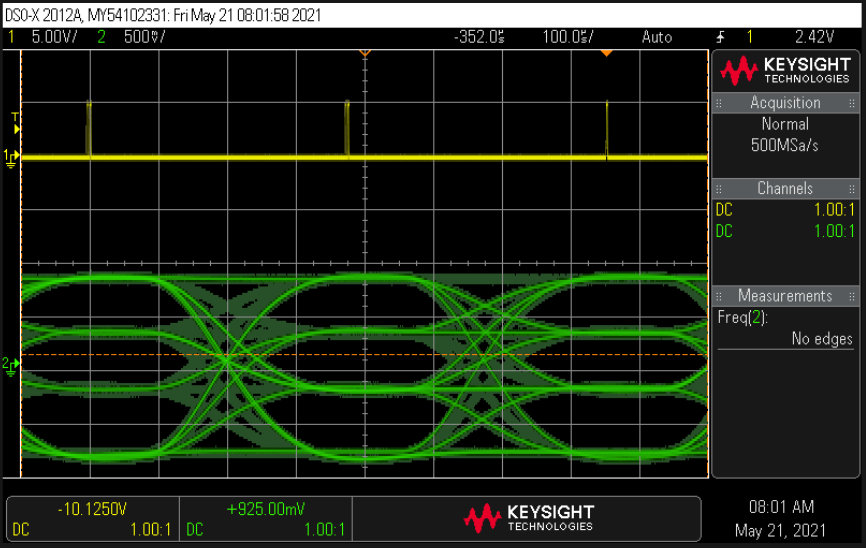
\includegraphics[width=0.8\textwidth]{scope.png}
    \caption{Oscilloscope output for signal generator \textbf{A}\label{scope}}
\end{figure}
\subsection{Steps required to generate image}
\begin{figure}[H]
    \centering
    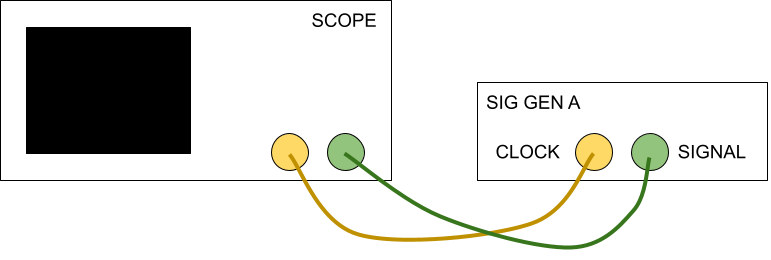
\includegraphics[width=0.8\textwidth]{scope_setup.png}
    \caption{Experiment setup}
\end{figure}
These steps can be used to generate an eye diagram on a generic digital storage
oscilloscope:
\begin{enumerate}
    \item Connect the signal and clock outputs of the signal generator to two
          input channels of the oscilloscope.
    \item Set the trigger of the oscilloscope to use the clock channel.
    \item Adjust the trigger level to approximately half of the maximum
          amplitude of the clock signal, about 2.5V in this case. Any trigger
          level such that the refresh is only triggered on the edge of a pulse
          will work (ie. not above the max amplitude but not below the noise
          threshold of a clock `0' output).
    \item Adjust the horizontal scaling factor of the oscilloscope such that
          about three clock pulses are visible in the oscilloscope output
          window.
    \item Adjust the vertical scaling of both the signal and clock waveforms so
          main features are visible and large enough to measure using the volts
          per division and grid.
    \item Turn the persistence of the oscilloscope to maximum ($\infty$)
    \item If the image needs to be adjusted (scaled or horizontally offset), the
          persistence must be cleared.
\end{enumerate}

\subsection{Modulation type}
As shown in \Cref{scope}, the signal output shows four main levels at the eye
open instant. These are levels of voltage (signal \textit{amplitude}). Because
of this, the modulation type is 4-PAM.

\subsection{Signal characteristics}
\paragraph{Symbol rate}
The symbol rate is the frequency at which symbols are transmitted, which can be
found by the reciprocal of the time between clock pulses. Measured at 2.66KHz.
\paragraph{Error free sampling interval}
The error free sampling interval is the horizontal distance between the
left-most and right-most corners of the eye. In this interval, the signal has
settled in to one of the threshold regions for symbol decoding and will be
correctly decoded. Measured at 260us.
\paragraph{Margin over noise}
Noise margin is the voltage difference between a threshold (the horizontal axis
of the eye) and the maximum value of a noisy signal at the widest opening point
of the eye. If the signal were to be distorted by more than this margin, it
would cause a bit error even with if the sampling instant was chosen optimally.
Measured at 200mV.
\paragraph{Level crossing timing jitter}
Level crossing jitter is the variation in when signals cross the threshold
level. It shows the clock stability of the transmitter or phase distortion in
the transmission medium. Measured at 120us.

\subsection{Sensitivity of signal to timing error}

\end{document}